\documentclass[twoside]{book}

% Packages required by doxygen
\usepackage{calc}
\usepackage{doxygen}
\usepackage{graphicx}
\usepackage[utf8]{inputenc}
\usepackage{makeidx}
\usepackage{multicol}
\usepackage{multirow}
\usepackage{textcomp}
\usepackage[table]{xcolor}

% Font selection
\usepackage[T1]{fontenc}
\usepackage{mathptmx}
\usepackage[scaled=.90]{helvet}
\usepackage{courier}
\usepackage{amssymb}
\usepackage{sectsty}
\renewcommand{\familydefault}{\sfdefault}
\allsectionsfont{%
  \fontseries{bc}\selectfont%
  \color{darkgray}%
}
\renewcommand{\DoxyLabelFont}{%
  \fontseries{bc}\selectfont%
  \color{darkgray}%
}

% Page & text layout
\usepackage{geometry}
\geometry{%
  a4paper,%
  top=2.5cm,%
  bottom=2.5cm,%
  left=2.5cm,%
  right=2.5cm%
}
\tolerance=750
\hfuzz=15pt
\hbadness=750
\setlength{\emergencystretch}{15pt}
\setlength{\parindent}{0cm}
\setlength{\parskip}{0.2cm}
\makeatletter
\renewcommand{\paragraph}{%
  \@startsection{paragraph}{4}{0ex}{-1.0ex}{1.0ex}{%
    \normalfont\normalsize\bfseries\SS@parafont%
  }%
}
\renewcommand{\subparagraph}{%
  \@startsection{subparagraph}{5}{0ex}{-1.0ex}{1.0ex}{%
    \normalfont\normalsize\bfseries\SS@subparafont%
  }%
}
\makeatother

% Headers & footers
\usepackage{fancyhdr}
\pagestyle{fancyplain}
\fancyhead[LE]{\fancyplain{}{\bfseries\thepage}}
\fancyhead[CE]{\fancyplain{}{}}
\fancyhead[RE]{\fancyplain{}{\bfseries\leftmark}}
\fancyhead[LO]{\fancyplain{}{\bfseries\rightmark}}
\fancyhead[CO]{\fancyplain{}{}}
\fancyhead[RO]{\fancyplain{}{\bfseries\thepage}}
\fancyfoot[LE]{\fancyplain{}{}}
\fancyfoot[CE]{\fancyplain{}{}}
\fancyfoot[RE]{\fancyplain{}{\bfseries\scriptsize Generated on Sat Jun 21 2014 17\-:17\-:23 for Motorcar by Doxygen }}
\fancyfoot[LO]{\fancyplain{}{\bfseries\scriptsize Generated on Sat Jun 21 2014 17\-:17\-:23 for Motorcar by Doxygen }}
\fancyfoot[CO]{\fancyplain{}{}}
\fancyfoot[RO]{\fancyplain{}{}}
\renewcommand{\footrulewidth}{0.4pt}
\renewcommand{\chaptermark}[1]{%
  \markboth{#1}{}%
}
\renewcommand{\sectionmark}[1]{%
  \markright{\thesection\ #1}%
}

% Indices & bibliography
\usepackage{natbib}
\usepackage[titles]{tocloft}
\setcounter{tocdepth}{3}
\setcounter{secnumdepth}{5}
\makeindex

% Hyperlinks (required, but should be loaded last)
\usepackage{ifpdf}
\ifpdf
  \usepackage[pdftex,pagebackref=true]{hyperref}
\else
  \usepackage[ps2pdf,pagebackref=true]{hyperref}
\fi
\hypersetup{%
  colorlinks=true,%
  linkcolor=blue,%
  citecolor=blue,%
  unicode%
}

% Custom commands
\newcommand{\clearemptydoublepage}{%
  \newpage{\pagestyle{empty}\cleardoublepage}%
}


%===== C O N T E N T S =====

\begin{document}

% Titlepage & ToC
\hypersetup{pageanchor=false}
\pagenumbering{roman}
\begin{titlepage}
\vspace*{7cm}
\begin{center}%
{\Large Motorcar }\\
\vspace*{1cm}
{\large Generated by Doxygen 1.8.6}\\
\vspace*{0.5cm}
{\small Sat Jun 21 2014 17:17:23}\\
\end{center}
\end{titlepage}
\clearemptydoublepage
\tableofcontents
\clearemptydoublepage
\pagenumbering{arabic}
\hypersetup{pageanchor=true}

%--- Begin generated contents ---
\chapter{Motorcar}
\label{md__home_dave_thesis_motorcar_README}
\hypertarget{md__home_dave_thesis_motorcar_README}{}
Motorcar is a framework for 3\-D windowing built on top of Wayland which I originally developed for my Master's thesis at Cal Poly (\href{https://github.com/evil0sheep/MastersThesis/blob/master/thesis.pdf?raw=true}{\tt pdf}, \href{https://docs.google.com/presentation/d/1svgGMxxbfmcHy_KuS5Q9hah8PQOsXqvjBKOoMIzW24Y/edit?usp=sharing}{\tt defense slides}). It is designed to provide basic 3\-D windowing infrastructure that gives 3\-D applications desktop flexibility in the how their 3\-D content is drawn while supporting unmodified Wayland applications in the same 3\-D compositor space, and to do this with the simplest mechanism possible.

Motorcar is free and open source (under the B\-S\-D license), and I am very open to contributions (both conceptual and functional) from the community. If you have any questions, comments, or critical feedback about the software, or if you are interested in using or contributing Motorcar, or if you are working on something related, please feel free to contact me, I would love to hear from you.

\section*{Building Motorcar }

In general if you are looking to build Motorcar you should pull the stable branch, as the master branch may periodically go into unbuildable states. Please note that the software in the stable branch is not guaranteed to {\itshape actually be} stable, but I will not knowingly commit broken code to stable.

If you have trouble building Motorcar or feedback regarding the build process please contact me. At the time of me writing these build instructions this software has not been built on another system to my knowledge, so there could be significant problems with the software or build system that I am simply unaware of.

\subsection*{Dependencies }

Motorcar has significant external dependencies, some of which may need to be built from source depending on your Linux distribution. These dependencies can be summarized at a high level as a dependency on the \href{http://qt-project.org/wiki/QtWayland}{\tt Qt\-Wayland Qt\-Compositor} module with support for E\-G\-L with desktop Open\-G\-L (not Open\-G\-L E\-S). This in turn requires \href{http://wayland.freedesktop.org/}{\tt Wayland}, which may be available as a package depending on your Linux distribution, or may need to be \href{http://wayland.freedesktop.org/building.html}{\tt built from source}, as well as support for E\-G\-L with desktop Open\-G\-L, which may require building Mesa from source. Instructions for building Mesa for Wayland E\-G\-L can be found in the \href{http://wayland.freedesktop.org/building.html}{\tt Wayland build instructions}. I use the following configurations\-:


\begin{DoxyItemize}
\item Mesa \begin{DoxyVerb}  $ autogen.sh --prefix=$WLD --enable-gles2 --disable-gallium-egl --with-egl-platforms=x11,wayland,drm --enable-gbm --enable-shared-glapi --with-gallium-drivers=r300,r600,swrast,nouveau --enable-glx-tls
\end{DoxyVerb}

\item Cairo \begin{DoxyVerb}  $ autogen.sh --prefix=$WLD --enable-xcb=yes --enable-gl=yes -enable-egl=yes
\end{DoxyVerb}

\end{DoxyItemize}

Build instructions for Qt\-Wayland can be found on the \href{http://qt-project.org/wiki/QtWayland}{\tt Qt\-Wayland page}, and these cover most everything needed to get build Qt\-Wayland. Getting it to work properly with E\-G\-L and desktop Open\-G\-L is a little bit tricky, and I have copied my build command below for reference, which I imagine will probably work on most systems, though this is of course not guaranteed.

Below are the hashes of the commits which I am currently using for the Qt dependencies, which I include mainly for reference since they are known to work together. Other combinations may work as well. Please note that qtbase and qtwayland are git submodules of the qt5 repository.


\begin{DoxyItemize}
\item Qt5\-:
\begin{DoxyItemize}
\item e198c124d3259dea657fcfa4c9b9b43bcd2d9fd0
\item The most recent commit might work here but if the version exceeds 5.\-3.\-0 you may run into problems with the Qt\-Wayland private includes
\end{DoxyItemize}
\item qtbase
\begin{DoxyItemize}
\item 625002f7067271b8f03f7bfa13baff6128c72e68
\item The most recent commit will probably work here
\end{DoxyItemize}
\item qtwayland
\begin{DoxyItemize}
\item 5c605d363e2fc42f5ec80413d093b69614027da4
\item This is the most likely to cause problems as the Compositor A\-P\-I changes quite frequently.
\end{DoxyItemize}
\end{DoxyItemize}

Here is the build sequence I use for Qt5 and Qt\-Wayland to get them to support E\-G\-L with desktop Open\-G\-L. Again, this is certainly not guaranteed to work on every system, it is included here mainly as a reference. Please refer to the \href{http://qt-project.org/wiki/Building_Qt_5_from_Git}{\tt Qt5 build instructions} and the \href{http://qt-project.org/wiki/QtWayland}{\tt Qt\-Wayland build instructions} for more information. \begin{DoxyVerb}$ git clone git://gitorious.org/qt/qt5.git qt5
$ cd qt5
$ git checkout e198c124d3259dea657fcfa4c9b9b43bcd2d9fd0
$ ./init-repository --no-webkit  --module-subset=qtbase,qtjsbackend,qtdeclarative,qtwayland
\end{DoxyVerb}


Other modules may be required to run some of the Qt clients, but not for Motorcar itself \begin{DoxyVerb}$ cd qtbase
$ git checkout 625002f7067271b8f03f7bfa13baff6128c72e68
$ cd ../qtwayland
$ git checkout 5c605d363e2fc42f5ec80413d093b69614027da4
$ cd ../
$ ./configure -prefix /opt/qt5  -debug -confirm-license -opensource -egl -opengl  -no-xcb-xlib
\end{DoxyVerb}


I install into opt/qt5, but this is not a hard requirement, just make sure that when you run qmake it is running the executable installed here. The -\/no-\/xcb-\/xlib argument is required to build against E\-G\-L and desktop Open\-G\-L in the commit listed above, but this may have been fixed in newer versions of Qt\-Wayland \begin{DoxyVerb}$ cd qtwayland
$ git clean -fdx
$ ../qtbase/bin/qmake CONFIG+=wayland-compositor
$ cd ../
$ make
$ make install
\end{DoxyVerb}


If this gives you trouble you might want to try making and installing Qt\-Wayland from the qtwayland subdirectory.

\subsection*{Building Motorcar Itself }

Motorcar is separated into several components, which are designed to be able to be used together or independently from one another. The Wayland protocol extensions used for 3\-D windowing and 3\-D input are specified in \href{https://github.com/evil0sheep/motorcar/blob/stable/src/protocol/motorcar.xml}{\tt motorcar.\-xml} and the language bingings used by the compositor and clients are generated when those components are compiled.

\subsubsection*{Building the Motorcar Compositor Library}

The compositor is built in two steps. The first step builds the Motorcar compositor library which contains the Wayland backend and Qt dependency, and most of the scenegraph and compositing logic. The second step builds the compositor itself, which is a lightweight program that essentially just uses the compositor library to set up the scene and insert devices into the scenegraph.

This allows many compositors to be built with the core windowing infrastructure, and allows developers implementing compositors to add support for their devices or to replace components of the windowing logic (like the window manager) with their own classes without those classes needing to be in the core Motorcar code base (though I am very open to pull requests). It also keeps device specific dependencies out of the core compositor code.

Currently the entire compositor library is built with qmake, but eventually I would like to transition to G\-N\-U autotools and only use qmake to build the Qt dependent components (since this is a relatively small portion of the code base). To build the motorcar compositor library\-: \begin{DoxyVerb}$ cd path/to/motorcar/repo
$ qmake
$ make
\end{DoxyVerb}


This will build shared objects in the lib directory (under the repository root directory) which compositors will link against when using the Motorcar compositor library.

\subsubsection*{Building the Example Compositor}

This repository contains an example compositor which uses an Oculus Rift as a 3\-D display and a Sixense/\-Razer Hydra as a 6\-Do\-F input device. Building this example compositor requires that both the Oculus\-V\-R S\-D\-K and the Sixense S\-D\-K be present in the system. To build the example compositor\-: \begin{DoxyVerb}$ cd path/to/motorcar/repo
$ cd src/examples/compositors/rift-hydra-compositor
$ make LIBOVRPATH=/path/to/LibOVR SIXENSEPATH=/path/to/sixenseSDK_linux_OSX
\end{DoxyVerb}


This will build an executable called rift-\/hydra-\/compositor in the current directory

In the future there will likely be more compositors, and possibly some mechanism for automatically detecting which device S\-D\-Ks are present and auto generating a compositor which reads in some kind of scene configuration file to control scene layout.

\subsubsection*{Building the Motorcar Demo Client}

This repository also contains an example client which supports the Motorcar protocol extensions for view-\/dependent depth-\/composited 3\-D rendering based on weston-\/simple-\/egl. Eventually this client will be broken apart into a client-\/side windowing library and example clients built with this library, similar to the compositor code, and when this happens these build instructions will be updated accordingly. To build the demo client \begin{DoxyVerb}$ cd path/to/motorcar/repo
$ cd src/examples/clients/simple-egl/
$ make 
\end{DoxyVerb}


This will build an executable called motorcar-\/demo-\/client in the current directory. This client takes several flags, most of which were inherited from weston-\/simple-\/egl. The -\/p flag enables portal clipping mode, rather than the default cuboid clipping mode, and the -\/d flag disables depth compositing on the 3\-D window. See \href{https://github.com/evil0sheep/MastersThesis/blob/master/thesis.pdf?raw=true}{\tt my thesis} and my \href{https://docs.google.com/presentation/d/1svgGMxxbfmcHy_KuS5Q9hah8PQOsXqvjBKOoMIzW24Y/edit?usp=sharing}{\tt thesis defense slides} for a conceptual explanation of what this means. 
\chapter{Namespace Index}
\section{Namespace List}
Here is a list of all namespaces with brief descriptions\-:\begin{DoxyCompactList}
\item\contentsline{section}{\hyperlink{namespacemotorcar}{motorcar} }{\pageref{namespacemotorcar}}{}
\item\contentsline{section}{\hyperlink{namespaceqtmotorcar}{qtmotorcar} }{\pageref{namespaceqtmotorcar}}{}
\end{DoxyCompactList}

\chapter{Hierarchical Index}
\section{Class Hierarchy}
This inheritance list is sorted roughly, but not completely, alphabetically\-:\begin{DoxyCompactList}
\item \contentsline{section}{motorcar\-:\-:Compositor}{\pageref{classmotorcar_1_1Compositor}}{}
\begin{DoxyCompactList}
\item \contentsline{section}{qtmotorcar\-:\-:Qt\-Wayland\-Motorcar\-Compositor}{\pageref{classqtmotorcar_1_1QtWaylandMotorcarCompositor}}{}
\end{DoxyCompactList}
\item \contentsline{section}{display}{\pageref{structdisplay}}{}
\item \contentsline{section}{motorcar\-:\-:Display\-Server}{\pageref{classmotorcar_1_1DisplayServer}}{}
\item \contentsline{section}{motorcar\-:\-:Event}{\pageref{classmotorcar_1_1Event}}{}
\begin{DoxyCompactList}
\item \contentsline{section}{motorcar\-:\-:Keyboard\-Event}{\pageref{classmotorcar_1_1KeyboardEvent}}{}
\item \contentsline{section}{motorcar\-:\-:Mouse\-Event}{\pageref{classmotorcar_1_1MouseEvent}}{}
\end{DoxyCompactList}
\item \contentsline{section}{motorcar\-:\-:Geometry}{\pageref{classmotorcar_1_1Geometry}}{}
\item \contentsline{section}{geometry}{\pageref{structgeometry}}{}
\item \contentsline{section}{Gl\-Buffer\-Object}{\pageref{classGlBufferObject}}{}
\item \contentsline{section}{motorcar\-:\-:Keyboard}{\pageref{classmotorcar_1_1Keyboard}}{}
\item \contentsline{section}{motorcar\-\_\-shell\-\_\-interface}{\pageref{structmotorcar__shell__interface}}{}
\item \contentsline{section}{motorcar\-\_\-viewpoint\-\_\-listener}{\pageref{structmotorcar__viewpoint__listener}}{}
\item \contentsline{section}{motorcar\-:\-:Open\-G\-L\-Context}{\pageref{classmotorcar_1_1OpenGLContext}}{}
\begin{DoxyCompactList}
\item \contentsline{section}{qtmotorcar\-:\-:Qt\-Wayland\-Motorcar\-Open\-G\-L\-Context}{\pageref{classqtmotorcar_1_1QtWaylandMotorcarOpenGLContext}}{}
\end{DoxyCompactList}
\item \contentsline{section}{Open\-G\-L\-Data}{\pageref{classOpenGLData}}{}
\item \contentsline{section}{motorcar\-:\-:Open\-G\-L\-Shader}{\pageref{classmotorcar_1_1OpenGLShader}}{}
\item \contentsline{section}{motorcar\-:\-:Geometry\-:\-:Plane}{\pageref{structmotorcar_1_1Geometry_1_1Plane}}{}
\item \contentsline{section}{motorcar\-:\-:Pointer}{\pageref{classmotorcar_1_1Pointer}}{}
\item Q\-Object\begin{DoxyCompactList}
\item \contentsline{section}{qtmotorcar\-:\-:Qt\-Wayland\-Motorcar\-Compositor}{\pageref{classqtmotorcar_1_1QtWaylandMotorcarCompositor}}{}
\end{DoxyCompactList}
\item \contentsline{section}{Qtwayland\-Surface\-Node}{\pageref{classQtwaylandSurfaceNode}}{}
\item Q\-Wayland\-Compositor\begin{DoxyCompactList}
\item \contentsline{section}{qtmotorcar\-:\-:Qt\-Wayland\-Motorcar\-Compositor}{\pageref{classqtmotorcar_1_1QtWaylandMotorcarCompositor}}{}
\end{DoxyCompactList}
\item Q\-Window\begin{DoxyCompactList}
\item \contentsline{section}{Q\-Open\-G\-L\-Window}{\pageref{classQOpenGLWindow}}{}
\end{DoxyCompactList}
\item \contentsline{section}{motorcar\-:\-:Geometry\-:\-:Ray}{\pageref{structmotorcar_1_1Geometry_1_1Ray}}{}
\item \contentsline{section}{motorcar\-:\-:Geometry\-:\-:Ray\-Surface\-Intersection}{\pageref{structmotorcar_1_1Geometry_1_1RaySurfaceIntersection}}{}
\item \contentsline{section}{motorcar\-:\-:Geometry\-:\-:Rectangle}{\pageref{structmotorcar_1_1Geometry_1_1Rectangle}}{}
\begin{DoxyCompactList}
\item \contentsline{section}{motorcar\-:\-:Display}{\pageref{classmotorcar_1_1Display}}{}
\begin{DoxyCompactList}
\item \contentsline{section}{motorcar\-:\-:Render\-To\-Texture\-Display}{\pageref{classmotorcar_1_1RenderToTextureDisplay}}{}
\begin{DoxyCompactList}
\item \contentsline{section}{motorcar\-:\-:Oculus\-H\-M\-D}{\pageref{classmotorcar_1_1OculusHMD}}{}
\end{DoxyCompactList}
\end{DoxyCompactList}
\item \contentsline{section}{motorcar\-:\-:View\-Port}{\pageref{classmotorcar_1_1ViewPort}}{}
\end{DoxyCompactList}
\item \contentsline{section}{motorcar\-:\-:Scene\-Graph\-Node}{\pageref{classmotorcar_1_1SceneGraphNode}}{}
\begin{DoxyCompactList}
\item \contentsline{section}{motorcar\-:\-:Physical\-Node}{\pageref{classmotorcar_1_1PhysicalNode}}{}
\begin{DoxyCompactList}
\item \contentsline{section}{motorcar\-:\-:Bone}{\pageref{classmotorcar_1_1Bone}}{}
\item \contentsline{section}{motorcar\-:\-:Bone\-Sensor}{\pageref{classmotorcar_1_1BoneSensor}}{}
\begin{DoxyCompactList}
\item \contentsline{section}{motorcar\-:\-:Single\-Bone\-Tracker}{\pageref{classmotorcar_1_1SingleBoneTracker}}{}
\end{DoxyCompactList}
\item \contentsline{section}{motorcar\-:\-:Display}{\pageref{classmotorcar_1_1Display}}{}
\item \contentsline{section}{motorcar\-:\-:Scene}{\pageref{classmotorcar_1_1Scene}}{}
\item \contentsline{section}{motorcar\-:\-:Sixense\-Base\-Node}{\pageref{classmotorcar_1_1SixenseBaseNode}}{}
\item \contentsline{section}{motorcar\-:\-:Sixense\-Controller\-Node}{\pageref{classmotorcar_1_1SixenseControllerNode}}{}
\item \contentsline{section}{motorcar\-:\-:Skeleton}{\pageref{classmotorcar_1_1Skeleton}}{}
\item \contentsline{section}{motorcar\-:\-:Spatial\-Pointing\-Device}{\pageref{classmotorcar_1_1SpatialPointingDevice}}{}
\end{DoxyCompactList}
\item \contentsline{section}{motorcar\-:\-:Virtual\-Node}{\pageref{classmotorcar_1_1VirtualNode}}{}
\begin{DoxyCompactList}
\item \contentsline{section}{motorcar\-:\-:Drawable}{\pageref{classmotorcar_1_1Drawable}}{}
\begin{DoxyCompactList}
\item \contentsline{section}{motorcar\-:\-:Soft\-Kinetic\-Depth\-Camera}{\pageref{classmotorcar_1_1SoftKineticDepthCamera}}{}
\item \contentsline{section}{motorcar\-:\-:Wayland\-Surface\-Node}{\pageref{classmotorcar_1_1WaylandSurfaceNode}}{}
\begin{DoxyCompactList}
\item \contentsline{section}{motorcar\-:\-:Depth\-Composited\-Surface\-Node}{\pageref{classmotorcar_1_1DepthCompositedSurfaceNode}}{}
\end{DoxyCompactList}
\item \contentsline{section}{motorcar\-:\-:Wireframe\-Node}{\pageref{classmotorcar_1_1WireframeNode}}{}
\end{DoxyCompactList}
\item \contentsline{section}{motorcar\-:\-:View\-Point}{\pageref{classmotorcar_1_1ViewPoint}}{}
\end{DoxyCompactList}
\end{DoxyCompactList}
\item \contentsline{section}{motorcar\-:\-:Seat}{\pageref{classmotorcar_1_1Seat}}{}
\begin{DoxyCompactList}
\item \contentsline{section}{qtmotorcar\-:\-:Qt\-Wayland\-Motorcar\-Seat}{\pageref{classqtmotorcar_1_1QtWaylandMotorcarSeat}}{}
\end{DoxyCompactList}
\item \contentsline{section}{motorcar\-:\-:Shell}{\pageref{classmotorcar_1_1Shell}}{}
\item \contentsline{section}{motorcar\-:\-:Sixense\-Motion\-Sensing\-System}{\pageref{classmotorcar_1_1SixenseMotionSensingSystem}}{}
\item \contentsline{section}{Texture\-Blitter}{\pageref{classTextureBlitter}}{}
\item \contentsline{section}{viewpoint}{\pageref{structviewpoint}}{}
\item \contentsline{section}{viewport}{\pageref{structviewport}}{}
\item \contentsline{section}{motorcar\-:\-:Wayland\-Surface}{\pageref{classmotorcar_1_1WaylandSurface}}{}
\begin{DoxyCompactList}
\item \contentsline{section}{qtmotorcar\-:\-:Qt\-Wayland\-Motorcar\-Surface}{\pageref{classqtmotorcar_1_1QtWaylandMotorcarSurface}}{}
\end{DoxyCompactList}
\item \contentsline{section}{window}{\pageref{structwindow}}{}
\item \contentsline{section}{motorcar\-:\-:Window\-Manager}{\pageref{classmotorcar_1_1WindowManager}}{}
\end{DoxyCompactList}

\chapter{Class Index}
\section{Class List}
Here are the classes, structs, unions and interfaces with brief descriptions\-:\begin{DoxyCompactList}
\item\contentsline{section}{\hyperlink{structmotorcar_1_1Geometry_1_1AxisAlignedBox}{motorcar\-::\-Geometry\-::\-Axis\-Aligned\-Box} }{\pageref{structmotorcar_1_1Geometry_1_1AxisAlignedBox}}{}
\item\contentsline{section}{\hyperlink{classmotorcar_1_1Bone}{motorcar\-::\-Bone} }{\pageref{classmotorcar_1_1Bone}}{}
\item\contentsline{section}{\hyperlink{classmotorcar_1_1BoneSensor}{motorcar\-::\-Bone\-Sensor} }{\pageref{classmotorcar_1_1BoneSensor}}{}
\item\contentsline{section}{\hyperlink{classBox}{Box} }{\pageref{classBox}}{}
\item\contentsline{section}{\hyperlink{classmotorcar_1_1Compositor}{motorcar\-::\-Compositor} \\*This class handles only the invoking the draw calls on the scenegraph needed to display its contents }{\pageref{classmotorcar_1_1Compositor}}{}
\item\contentsline{section}{\hyperlink{structdisplay}{display} }{\pageref{structdisplay}}{}
\item\contentsline{section}{\hyperlink{classmotorcar_1_1Display}{motorcar\-::\-Display} }{\pageref{classmotorcar_1_1Display}}{}
\item\contentsline{section}{\hyperlink{classmotorcar_1_1DisplayServer}{motorcar\-::\-Display\-Server} \\*This class handles client connection/disconnection and most of the direct wayland interactions }{\pageref{classmotorcar_1_1DisplayServer}}{}
\item\contentsline{section}{\hyperlink{classmotorcar_1_1Drawable}{motorcar\-::\-Drawable} }{\pageref{classmotorcar_1_1Drawable}}{}
\item\contentsline{section}{\hyperlink{classmotorcar_1_1Event}{motorcar\-::\-Event} }{\pageref{classmotorcar_1_1Event}}{}
\item\contentsline{section}{\hyperlink{structgeometry}{geometry} }{\pageref{structgeometry}}{}
\item\contentsline{section}{\hyperlink{classmotorcar_1_1Geometry}{motorcar\-::\-Geometry} }{\pageref{classmotorcar_1_1Geometry}}{}
\item\contentsline{section}{\hyperlink{classGlBufferObject}{Gl\-Buffer\-Object} }{\pageref{classGlBufferObject}}{}
\item\contentsline{section}{\hyperlink{classmotorcar_1_1Keyboard}{motorcar\-::\-Keyboard} }{\pageref{classmotorcar_1_1Keyboard}}{}
\item\contentsline{section}{\hyperlink{classmotorcar_1_1KeyboardEvent}{motorcar\-::\-Keyboard\-Event} }{\pageref{classmotorcar_1_1KeyboardEvent}}{}
\item\contentsline{section}{\hyperlink{structmotorcar__shell__interface}{motorcar\-\_\-shell\-\_\-interface} }{\pageref{structmotorcar__shell__interface}}{}
\item\contentsline{section}{\hyperlink{structmotorcar__six__dof__pointer__interface}{motorcar\-\_\-six\-\_\-dof\-\_\-pointer\-\_\-interface} }{\pageref{structmotorcar__six__dof__pointer__interface}}{}
\item\contentsline{section}{\hyperlink{structmotorcar__six__dof__pointer__listener}{motorcar\-\_\-six\-\_\-dof\-\_\-pointer\-\_\-listener} }{\pageref{structmotorcar__six__dof__pointer__listener}}{}
\item\contentsline{section}{\hyperlink{structmotorcar__surface__interface}{motorcar\-\_\-surface\-\_\-interface} }{\pageref{structmotorcar__surface__interface}}{}
\item\contentsline{section}{\hyperlink{structmotorcar__surface__listener}{motorcar\-\_\-surface\-\_\-listener} }{\pageref{structmotorcar__surface__listener}}{}
\item\contentsline{section}{\hyperlink{structmotorcar__viewpoint__listener}{motorcar\-\_\-viewpoint\-\_\-listener} }{\pageref{structmotorcar__viewpoint__listener}}{}
\item\contentsline{section}{\hyperlink{classmotorcar_1_1MotorcarSurfaceNode}{motorcar\-::\-Motorcar\-Surface\-Node} }{\pageref{classmotorcar_1_1MotorcarSurfaceNode}}{}
\item\contentsline{section}{\hyperlink{structmotorsurface__listener}{motorsurface\-\_\-listener} }{\pageref{structmotorsurface__listener}}{}
\item\contentsline{section}{\hyperlink{classmotorcar_1_1MouseEvent}{motorcar\-::\-Mouse\-Event} }{\pageref{classmotorcar_1_1MouseEvent}}{}
\item\contentsline{section}{\hyperlink{classmotorcar_1_1OculusHMD}{motorcar\-::\-Oculus\-H\-M\-D} }{\pageref{classmotorcar_1_1OculusHMD}}{}
\item\contentsline{section}{\hyperlink{classmotorcar_1_1OpenGLContext}{motorcar\-::\-Open\-G\-L\-Context} }{\pageref{classmotorcar_1_1OpenGLContext}}{}
\item\contentsline{section}{\hyperlink{classOpenGLData}{Open\-G\-L\-Data} }{\pageref{classOpenGLData}}{}
\item\contentsline{section}{\hyperlink{classmotorcar_1_1OpenGLShader}{motorcar\-::\-Open\-G\-L\-Shader} }{\pageref{classmotorcar_1_1OpenGLShader}}{}
\item\contentsline{section}{\hyperlink{classmotorcar_1_1PhysicalNode}{motorcar\-::\-Physical\-Node} }{\pageref{classmotorcar_1_1PhysicalNode}}{}
\item\contentsline{section}{\hyperlink{structmotorcar_1_1Geometry_1_1Plane}{motorcar\-::\-Geometry\-::\-Plane} }{\pageref{structmotorcar_1_1Geometry_1_1Plane}}{}
\item\contentsline{section}{\hyperlink{classmotorcar_1_1Pointer}{motorcar\-::\-Pointer} }{\pageref{classmotorcar_1_1Pointer}}{}
\item\contentsline{section}{\hyperlink{classQOpenGLWindow}{Q\-Open\-G\-L\-Window} }{\pageref{classQOpenGLWindow}}{}
\item\contentsline{section}{\hyperlink{classqtmotorcar_1_1QtWaylandMotorcarCompositor}{qtmotorcar\-::\-Qt\-Wayland\-Motorcar\-Compositor} }{\pageref{classqtmotorcar_1_1QtWaylandMotorcarCompositor}}{}
\item\contentsline{section}{\hyperlink{classqtmotorcar_1_1QtWaylandMotorcarOpenGLContext}{qtmotorcar\-::\-Qt\-Wayland\-Motorcar\-Open\-G\-L\-Context} }{\pageref{classqtmotorcar_1_1QtWaylandMotorcarOpenGLContext}}{}
\item\contentsline{section}{\hyperlink{classqtmotorcar_1_1QtWaylandMotorcarSeat}{qtmotorcar\-::\-Qt\-Wayland\-Motorcar\-Seat} }{\pageref{classqtmotorcar_1_1QtWaylandMotorcarSeat}}{}
\item\contentsline{section}{\hyperlink{classqtmotorcar_1_1QtWaylandMotorcarSurface}{qtmotorcar\-::\-Qt\-Wayland\-Motorcar\-Surface} }{\pageref{classqtmotorcar_1_1QtWaylandMotorcarSurface}}{}
\item\contentsline{section}{\hyperlink{classQtwaylandSurfaceNode}{Qtwayland\-Surface\-Node} }{\pageref{classQtwaylandSurfaceNode}}{}
\item\contentsline{section}{\hyperlink{structmotorcar_1_1Geometry_1_1Ray}{motorcar\-::\-Geometry\-::\-Ray} }{\pageref{structmotorcar_1_1Geometry_1_1Ray}}{}
\item\contentsline{section}{\hyperlink{structmotorcar_1_1Geometry_1_1RaySurfaceIntersection}{motorcar\-::\-Geometry\-::\-Ray\-Surface\-Intersection} }{\pageref{structmotorcar_1_1Geometry_1_1RaySurfaceIntersection}}{}
\item\contentsline{section}{\hyperlink{structmotorcar_1_1Geometry_1_1Rectangle}{motorcar\-::\-Geometry\-::\-Rectangle} }{\pageref{structmotorcar_1_1Geometry_1_1Rectangle}}{}
\item\contentsline{section}{\hyperlink{classmotorcar_1_1RenderToTextureDisplay}{motorcar\-::\-Render\-To\-Texture\-Display} }{\pageref{classmotorcar_1_1RenderToTextureDisplay}}{}
\item\contentsline{section}{\hyperlink{classmotorcar_1_1Scene}{motorcar\-::\-Scene} }{\pageref{classmotorcar_1_1Scene}}{}
\item\contentsline{section}{\hyperlink{classmotorcar_1_1SceneGraphNode}{motorcar\-::\-Scene\-Graph\-Node} }{\pageref{classmotorcar_1_1SceneGraphNode}}{}
\item\contentsline{section}{\hyperlink{classmotorcar_1_1Seat}{motorcar\-::\-Seat} }{\pageref{classmotorcar_1_1Seat}}{}
\item\contentsline{section}{\hyperlink{classmotorcar_1_1Shell}{motorcar\-::\-Shell} }{\pageref{classmotorcar_1_1Shell}}{}
\item\contentsline{section}{\hyperlink{classmotorcar_1_1SingleBoneTracker}{motorcar\-::\-Single\-Bone\-Tracker} }{\pageref{classmotorcar_1_1SingleBoneTracker}}{}
\item\contentsline{section}{\hyperlink{classmotorcar_1_1SixDofEvent}{motorcar\-::\-Six\-Dof\-Event} }{\pageref{classmotorcar_1_1SixDofEvent}}{}
\item\contentsline{section}{\hyperlink{classsixDofPointer}{six\-Dof\-Pointer} }{\pageref{classsixDofPointer}}{}
\item\contentsline{section}{\hyperlink{classmotorcar_1_1SixDOFPointingDevice}{motorcar\-::\-Six\-D\-O\-F\-Pointing\-Device} }{\pageref{classmotorcar_1_1SixDOFPointingDevice}}{}
\item\contentsline{section}{\hyperlink{classmotorcar_1_1SixenseBaseNode}{motorcar\-::\-Sixense\-Base\-Node} }{\pageref{classmotorcar_1_1SixenseBaseNode}}{}
\item\contentsline{section}{\hyperlink{classmotorcar_1_1SixenseControllerNode}{motorcar\-::\-Sixense\-Controller\-Node} }{\pageref{classmotorcar_1_1SixenseControllerNode}}{}
\item\contentsline{section}{\hyperlink{classmotorcar_1_1SixenseMotionSensingSystem}{motorcar\-::\-Sixense\-Motion\-Sensing\-System} }{\pageref{classmotorcar_1_1SixenseMotionSensingSystem}}{}
\item\contentsline{section}{\hyperlink{classmotorcar_1_1Skeleton}{motorcar\-::\-Skeleton} }{\pageref{classmotorcar_1_1Skeleton}}{}
\item\contentsline{section}{\hyperlink{classmotorcar_1_1SoftKineticDepthCamera}{motorcar\-::\-Soft\-Kinetic\-Depth\-Camera} }{\pageref{classmotorcar_1_1SoftKineticDepthCamera}}{}
\item\contentsline{section}{\hyperlink{classTextureBlitter}{Texture\-Blitter} }{\pageref{classTextureBlitter}}{}
\item\contentsline{section}{\hyperlink{structviewpoint}{viewpoint} }{\pageref{structviewpoint}}{}
\item\contentsline{section}{\hyperlink{classmotorcar_1_1ViewPoint}{motorcar\-::\-View\-Point} }{\pageref{classmotorcar_1_1ViewPoint}}{}
\item\contentsline{section}{\hyperlink{classmotorcar_1_1ViewPort}{motorcar\-::\-View\-Port} }{\pageref{classmotorcar_1_1ViewPort}}{}
\item\contentsline{section}{\hyperlink{structviewport}{viewport} }{\pageref{structviewport}}{}
\item\contentsline{section}{\hyperlink{classmotorcar_1_1VirtualNode}{motorcar\-::\-Virtual\-Node} }{\pageref{classmotorcar_1_1VirtualNode}}{}
\item\contentsline{section}{\hyperlink{classmotorcar_1_1WaylandSurface}{motorcar\-::\-Wayland\-Surface} }{\pageref{classmotorcar_1_1WaylandSurface}}{}
\item\contentsline{section}{\hyperlink{classmotorcar_1_1WaylandSurfaceNode}{motorcar\-::\-Wayland\-Surface\-Node} }{\pageref{classmotorcar_1_1WaylandSurfaceNode}}{}
\item\contentsline{section}{\hyperlink{structwindow}{window} }{\pageref{structwindow}}{}
\item\contentsline{section}{\hyperlink{classmotorcar_1_1WindowManager}{motorcar\-::\-Window\-Manager} \\*Handles input events and window positioning }{\pageref{classmotorcar_1_1WindowManager}}{}
\item\contentsline{section}{\hyperlink{classmotorcar_1_1WireframeNode}{motorcar\-::\-Wireframe\-Node} }{\pageref{classmotorcar_1_1WireframeNode}}{}
\end{DoxyCompactList}

\chapter{File Index}
\section{File List}
Here is a list of all files with brief descriptions\-:\begin{DoxyCompactList}
\item\contentsline{section}{/home/dave/thesis/qtwayland-\/motorcar-\/compositor/motorcar/src/\hyperlink{compositor_8cpp}{compositor.\-cpp} }{\pageref{compositor_8cpp}}{}
\item\contentsline{section}{/home/dave/thesis/qtwayland-\/motorcar-\/compositor/motorcar/src/\hyperlink{compositor_8h}{compositor.\-h} }{\pageref{compositor_8h}}{}
\item\contentsline{section}{/home/dave/thesis/qtwayland-\/motorcar-\/compositor/motorcar/src/\hyperlink{geometry_8cpp}{geometry.\-cpp} }{\pageref{geometry_8cpp}}{}
\item\contentsline{section}{/home/dave/thesis/qtwayland-\/motorcar-\/compositor/motorcar/src/\hyperlink{geometry_8h}{geometry.\-h} }{\pageref{geometry_8h}}{}
\item\contentsline{section}{/home/dave/thesis/qtwayland-\/motorcar-\/compositor/motorcar/src/\hyperlink{motorcar_8h}{motorcar.\-h} }{\pageref{motorcar_8h}}{}
\item\contentsline{section}{/home/dave/thesis/qtwayland-\/motorcar-\/compositor/motorcar/src/device/\hyperlink{device_8h}{device.\-h} }{\pageref{device_8h}}{}
\item\contentsline{section}{/home/dave/thesis/qtwayland-\/motorcar-\/compositor/motorcar/src/device/\hyperlink{oculushmd_8cpp}{oculushmd.\-cpp} }{\pageref{oculushmd_8cpp}}{}
\item\contentsline{section}{/home/dave/thesis/qtwayland-\/motorcar-\/compositor/motorcar/src/device/\hyperlink{oculushmd_8h}{oculushmd.\-h} }{\pageref{oculushmd_8h}}{}
\item\contentsline{section}{/home/dave/thesis/qtwayland-\/motorcar-\/compositor/motorcar/src/device/\hyperlink{sixensebasenode_8cpp}{sixensebasenode.\-cpp} }{\pageref{sixensebasenode_8cpp}}{}
\item\contentsline{section}{/home/dave/thesis/qtwayland-\/motorcar-\/compositor/motorcar/src/device/\hyperlink{sixensebasenode_8h}{sixensebasenode.\-h} }{\pageref{sixensebasenode_8h}}{}
\item\contentsline{section}{/home/dave/thesis/qtwayland-\/motorcar-\/compositor/motorcar/src/device/\hyperlink{sixensecontrollernode_8cpp}{sixensecontrollernode.\-cpp} }{\pageref{sixensecontrollernode_8cpp}}{}
\item\contentsline{section}{/home/dave/thesis/qtwayland-\/motorcar-\/compositor/motorcar/src/device/\hyperlink{sixensecontrollernode_8h}{sixensecontrollernode.\-h} }{\pageref{sixensecontrollernode_8h}}{}
\item\contentsline{section}{/home/dave/thesis/qtwayland-\/motorcar-\/compositor/motorcar/src/device/\hyperlink{sixensemotionsensingsystem_8cpp}{sixensemotionsensingsystem.\-cpp} }{\pageref{sixensemotionsensingsystem_8cpp}}{}
\item\contentsline{section}{/home/dave/thesis/qtwayland-\/motorcar-\/compositor/motorcar/src/device/\hyperlink{sixensemotionsensingsystem_8h}{sixensemotionsensingsystem.\-h} }{\pageref{sixensemotionsensingsystem_8h}}{}
\item\contentsline{section}{/home/dave/thesis/qtwayland-\/motorcar-\/compositor/motorcar/src/gl/\hyperlink{GLSLHelper_8cpp}{G\-L\-S\-L\-Helper.\-cpp} }{\pageref{GLSLHelper_8cpp}}{}
\item\contentsline{section}{/home/dave/thesis/qtwayland-\/motorcar-\/compositor/motorcar/src/gl/\hyperlink{GLSLHelper_8h}{G\-L\-S\-L\-Helper.\-h} }{\pageref{GLSLHelper_8h}}{}
\item\contentsline{section}{/home/dave/thesis/qtwayland-\/motorcar-\/compositor/motorcar/src/gl/\hyperlink{openglcontext_8cpp}{openglcontext.\-cpp} }{\pageref{openglcontext_8cpp}}{}
\item\contentsline{section}{/home/dave/thesis/qtwayland-\/motorcar-\/compositor/motorcar/src/gl/\hyperlink{openglcontext_8h}{openglcontext.\-h} }{\pageref{openglcontext_8h}}{}
\item\contentsline{section}{/home/dave/thesis/qtwayland-\/motorcar-\/compositor/motorcar/src/gl/\hyperlink{openglshader_8cpp}{openglshader.\-cpp} }{\pageref{openglshader_8cpp}}{}
\item\contentsline{section}{/home/dave/thesis/qtwayland-\/motorcar-\/compositor/motorcar/src/gl/\hyperlink{openglshader_8h}{openglshader.\-h} }{\pageref{openglshader_8h}}{}
\item\contentsline{section}{/home/dave/thesis/qtwayland-\/motorcar-\/compositor/motorcar/src/scenegraph/\hyperlink{foo_8h}{foo.\-h} }{\pageref{foo_8h}}{}
\item\contentsline{section}{/home/dave/thesis/qtwayland-\/motorcar-\/compositor/motorcar/src/scenegraph/\hyperlink{ioelement_8cpp}{ioelement.\-cpp} }{\pageref{ioelement_8cpp}}{}
\item\contentsline{section}{/home/dave/thesis/qtwayland-\/motorcar-\/compositor/motorcar/src/scenegraph/\hyperlink{ioelement_8h}{ioelement.\-h} }{\pageref{ioelement_8h}}{}
\item\contentsline{section}{/home/dave/thesis/qtwayland-\/motorcar-\/compositor/motorcar/src/scenegraph/\hyperlink{physicalnode_8cpp}{physicalnode.\-cpp} }{\pageref{physicalnode_8cpp}}{}
\item\contentsline{section}{/home/dave/thesis/qtwayland-\/motorcar-\/compositor/motorcar/src/scenegraph/\hyperlink{physicalnode_8h}{physicalnode.\-h} }{\pageref{physicalnode_8h}}{}
\item\contentsline{section}{/home/dave/thesis/qtwayland-\/motorcar-\/compositor/motorcar/src/scenegraph/\hyperlink{scene_8cpp}{scene.\-cpp} }{\pageref{scene_8cpp}}{}
\item\contentsline{section}{/home/dave/thesis/qtwayland-\/motorcar-\/compositor/motorcar/src/scenegraph/\hyperlink{scene_8h}{scene.\-h} }{\pageref{scene_8h}}{}
\item\contentsline{section}{/home/dave/thesis/qtwayland-\/motorcar-\/compositor/motorcar/src/scenegraph/\hyperlink{scenegraph_8h}{scenegraph.\-h} }{\pageref{scenegraph_8h}}{}
\item\contentsline{section}{/home/dave/thesis/qtwayland-\/motorcar-\/compositor/motorcar/src/scenegraph/\hyperlink{scenegraphnode_8cpp}{scenegraphnode.\-cpp} }{\pageref{scenegraphnode_8cpp}}{}
\item\contentsline{section}{/home/dave/thesis/qtwayland-\/motorcar-\/compositor/motorcar/src/scenegraph/\hyperlink{scenegraphnode_8h}{scenegraphnode.\-h} }{\pageref{scenegraphnode_8h}}{}
\item\contentsline{section}{/home/dave/thesis/qtwayland-\/motorcar-\/compositor/motorcar/src/scenegraph/\hyperlink{virtualnode_8cpp}{virtualnode.\-cpp} }{\pageref{virtualnode_8cpp}}{}
\item\contentsline{section}{/home/dave/thesis/qtwayland-\/motorcar-\/compositor/motorcar/src/scenegraph/\hyperlink{virtualnode_8h}{virtualnode.\-h} }{\pageref{virtualnode_8h}}{}
\item\contentsline{section}{/home/dave/thesis/qtwayland-\/motorcar-\/compositor/motorcar/src/scenegraph/input/\hyperlink{inputelement_8cpp}{inputelement.\-cpp} }{\pageref{inputelement_8cpp}}{}
\item\contentsline{section}{/home/dave/thesis/qtwayland-\/motorcar-\/compositor/motorcar/src/scenegraph/input/\hyperlink{inputelement_8h}{inputelement.\-h} }{\pageref{inputelement_8h}}{}
\item\contentsline{section}{/home/dave/thesis/qtwayland-\/motorcar-\/compositor/motorcar/src/scenegraph/input/\hyperlink{spatialpointingdevice_8cpp}{spatialpointingdevice.\-cpp} }{\pageref{spatialpointingdevice_8cpp}}{}
\item\contentsline{section}{/home/dave/thesis/qtwayland-\/motorcar-\/compositor/motorcar/src/scenegraph/input/\hyperlink{spatialpointingdevice_8h}{spatialpointingdevice.\-h} }{\pageref{spatialpointingdevice_8h}}{}
\item\contentsline{section}{/home/dave/thesis/qtwayland-\/motorcar-\/compositor/motorcar/src/scenegraph/output/\hyperlink{drawable_8cpp}{drawable.\-cpp} }{\pageref{drawable_8cpp}}{}
\item\contentsline{section}{/home/dave/thesis/qtwayland-\/motorcar-\/compositor/motorcar/src/scenegraph/output/\hyperlink{drawable_8h}{drawable.\-h} }{\pageref{drawable_8h}}{}
\item\contentsline{section}{/home/dave/thesis/qtwayland-\/motorcar-\/compositor/motorcar/src/scenegraph/output/\hyperlink{glcameranode_8cpp}{glcameranode.\-cpp} }{\pageref{glcameranode_8cpp}}{}
\item\contentsline{section}{/home/dave/thesis/qtwayland-\/motorcar-\/compositor/motorcar/src/scenegraph/output/\hyperlink{glcameranode_8h}{glcameranode.\-h} }{\pageref{glcameranode_8h}}{}
\item\contentsline{section}{/home/dave/thesis/qtwayland-\/motorcar-\/compositor/motorcar/src/scenegraph/output/\hyperlink{output_8h}{output.\-h} }{\pageref{output_8h}}{}
\item\contentsline{section}{/home/dave/thesis/qtwayland-\/motorcar-\/compositor/motorcar/src/scenegraph/output/\hyperlink{outputelement_8cpp}{outputelement.\-cpp} }{\pageref{outputelement_8cpp}}{}
\item\contentsline{section}{/home/dave/thesis/qtwayland-\/motorcar-\/compositor/motorcar/src/scenegraph/output/\hyperlink{outputelement_8h}{outputelement.\-h} }{\pageref{outputelement_8h}}{}
\item\contentsline{section}{/home/dave/thesis/qtwayland-\/motorcar-\/compositor/motorcar/src/scenegraph/output/\hyperlink{wireframenode_8cpp}{wireframenode.\-cpp} }{\pageref{wireframenode_8cpp}}{}
\item\contentsline{section}{/home/dave/thesis/qtwayland-\/motorcar-\/compositor/motorcar/src/scenegraph/output/\hyperlink{wireframenode_8h}{wireframenode.\-h} }{\pageref{wireframenode_8h}}{}
\item\contentsline{section}{/home/dave/thesis/qtwayland-\/motorcar-\/compositor/motorcar/src/scenegraph/output/display/\hyperlink{display_8cpp}{display.\-cpp} }{\pageref{display_8cpp}}{}
\item\contentsline{section}{/home/dave/thesis/qtwayland-\/motorcar-\/compositor/motorcar/src/scenegraph/output/display/\hyperlink{display_8h}{display.\-h} }{\pageref{display_8h}}{}
\item\contentsline{section}{/home/dave/thesis/qtwayland-\/motorcar-\/compositor/motorcar/src/scenegraph/output/display/\hyperlink{rendertotexturedisplay_8cpp}{rendertotexturedisplay.\-cpp} }{\pageref{rendertotexturedisplay_8cpp}}{}
\item\contentsline{section}{/home/dave/thesis/qtwayland-\/motorcar-\/compositor/motorcar/src/scenegraph/output/display/\hyperlink{rendertotexturedisplay_8h}{rendertotexturedisplay.\-h} }{\pageref{rendertotexturedisplay_8h}}{}
\item\contentsline{section}{/home/dave/thesis/qtwayland-\/motorcar-\/compositor/motorcar/src/scenegraph/output/wayland/\hyperlink{waylanddrawable_8cpp}{waylanddrawable.\-cpp} }{\pageref{waylanddrawable_8cpp}}{}
\item\contentsline{section}{/home/dave/thesis/qtwayland-\/motorcar-\/compositor/motorcar/src/scenegraph/output/wayland/\hyperlink{waylanddrawable_8h}{waylanddrawable.\-h} }{\pageref{waylanddrawable_8h}}{}
\item\contentsline{section}{/home/dave/thesis/qtwayland-\/motorcar-\/compositor/motorcar/src/scenegraph/output/wayland/\hyperlink{waylandsurface_8cpp}{waylandsurface.\-cpp} }{\pageref{waylandsurface_8cpp}}{}
\item\contentsline{section}{/home/dave/thesis/qtwayland-\/motorcar-\/compositor/motorcar/src/scenegraph/output/wayland/\hyperlink{waylandsurface_8h}{waylandsurface.\-h} }{\pageref{waylandsurface_8h}}{}
\item\contentsline{section}{/home/dave/thesis/qtwayland-\/motorcar-\/compositor/motorcar/src/scenegraph/output/wayland/\hyperlink{waylandsurfacenode_8cpp}{waylandsurfacenode.\-cpp} }{\pageref{waylandsurfacenode_8cpp}}{}
\item\contentsline{section}{/home/dave/thesis/qtwayland-\/motorcar-\/compositor/motorcar/src/scenegraph/output/wayland/\hyperlink{waylandsurfacenode_8h}{waylandsurfacenode.\-h} }{\pageref{waylandsurfacenode_8h}}{}
\item\contentsline{section}{/home/dave/thesis/qtwayland-\/motorcar-\/compositor/qt/src/\hyperlink{opengldata_8cpp}{opengldata.\-cpp} }{\pageref{opengldata_8cpp}}{}
\item\contentsline{section}{/home/dave/thesis/qtwayland-\/motorcar-\/compositor/qt/src/\hyperlink{opengldata_8h}{opengldata.\-h} }{\pageref{opengldata_8h}}{}
\item\contentsline{section}{/home/dave/thesis/qtwayland-\/motorcar-\/compositor/qt/src/\hyperlink{qopenglwindow_8cpp}{qopenglwindow.\-cpp} }{\pageref{qopenglwindow_8cpp}}{}
\item\contentsline{section}{/home/dave/thesis/qtwayland-\/motorcar-\/compositor/qt/src/\hyperlink{qopenglwindow_8h}{qopenglwindow.\-h} }{\pageref{qopenglwindow_8h}}{}
\item\contentsline{section}{/home/dave/thesis/qtwayland-\/motorcar-\/compositor/qt/src/\hyperlink{qtwaylandmotorcarcompositor_8cpp}{qtwaylandmotorcarcompositor.\-cpp} }{\pageref{qtwaylandmotorcarcompositor_8cpp}}{}
\item\contentsline{section}{/home/dave/thesis/qtwayland-\/motorcar-\/compositor/qt/src/\hyperlink{qtwaylandmotorcarcompositor_8h}{qtwaylandmotorcarcompositor.\-h} }{\pageref{qtwaylandmotorcarcompositor_8h}}{}
\item\contentsline{section}{/home/dave/thesis/qtwayland-\/motorcar-\/compositor/qt/src/\hyperlink{qtwaylandmotorcaropenglcontext_8cpp}{qtwaylandmotorcaropenglcontext.\-cpp} }{\pageref{qtwaylandmotorcaropenglcontext_8cpp}}{}
\item\contentsline{section}{/home/dave/thesis/qtwayland-\/motorcar-\/compositor/qt/src/\hyperlink{qtwaylandmotorcaropenglcontext_8h}{qtwaylandmotorcaropenglcontext.\-h} }{\pageref{qtwaylandmotorcaropenglcontext_8h}}{}
\item\contentsline{section}{/home/dave/thesis/qtwayland-\/motorcar-\/compositor/qt/src/\hyperlink{qtwaylandmotorcarsurface_8cpp}{qtwaylandmotorcarsurface.\-cpp} }{\pageref{qtwaylandmotorcarsurface_8cpp}}{}
\item\contentsline{section}{/home/dave/thesis/qtwayland-\/motorcar-\/compositor/qt/src/\hyperlink{qtwaylandmotorcarsurface_8h}{qtwaylandmotorcarsurface.\-h} }{\pageref{qtwaylandmotorcarsurface_8h}}{}
\item\contentsline{section}{/home/dave/thesis/qtwayland-\/motorcar-\/compositor/qt/src/\hyperlink{qtwaylandsurfacenode_8cpp}{qtwaylandsurfacenode.\-cpp} }{\pageref{qtwaylandsurfacenode_8cpp}}{}
\item\contentsline{section}{/home/dave/thesis/qtwayland-\/motorcar-\/compositor/qt/src/\hyperlink{qtwaylandsurfacenode_8h}{qtwaylandsurfacenode.\-h} }{\pageref{qtwaylandsurfacenode_8h}}{}
\item\contentsline{section}{/home/dave/thesis/qtwayland-\/motorcar-\/compositor/qt/src/\hyperlink{textureblitter_8cpp}{textureblitter.\-cpp} }{\pageref{textureblitter_8cpp}}{}
\item\contentsline{section}{/home/dave/thesis/qtwayland-\/motorcar-\/compositor/qt/src/\hyperlink{textureblitter_8h}{textureblitter.\-h} }{\pageref{textureblitter_8h}}{}
\item\contentsline{section}{/home/dave/thesis/qtwayland-\/motorcar-\/compositor/src/\hyperlink{main_8cpp}{main.\-cpp} }{\pageref{main_8cpp}}{}
\end{DoxyCompactList}

\chapter{Namespace Documentation}
\hypertarget{namespacemotorcar}{\section{motorcar Namespace Reference}
\label{namespacemotorcar}\index{motorcar@{motorcar}}
}
\subsection*{Classes}
\begin{DoxyCompactItemize}
\item 
class \hyperlink{classmotorcar_1_1Compositor}{Compositor}
\begin{DoxyCompactList}\small\item\em This class handles only the invoking the draw calls on the scenegraph needed to display its contents. \end{DoxyCompactList}\item 
class \hyperlink{classmotorcar_1_1DisplayServer}{Display\-Server}
\begin{DoxyCompactList}\small\item\em This class handles client connection/disconnection and most of the direct wayland interactions. \end{DoxyCompactList}\item 
class \hyperlink{classmotorcar_1_1Event}{Event}
\item 
class \hyperlink{classmotorcar_1_1KeyboardEvent}{Keyboard\-Event}
\item 
class \hyperlink{classmotorcar_1_1MouseEvent}{Mouse\-Event}
\item 
class \hyperlink{classmotorcar_1_1SixDofEvent}{Six\-Dof\-Event}
\item 
class \hyperlink{classmotorcar_1_1Geometry}{Geometry}
\item 
class \hyperlink{classmotorcar_1_1OpenGLContext}{Open\-G\-L\-Context}
\item 
class \hyperlink{classmotorcar_1_1OpenGLShader}{Open\-G\-L\-Shader}
\item 
class \hyperlink{classmotorcar_1_1ViewPort}{View\-Port}
\item 
class \hyperlink{classmotorcar_1_1Bone}{Bone}
\item 
class \hyperlink{classmotorcar_1_1BoneSensor}{Bone\-Sensor}
\item 
class \hyperlink{classmotorcar_1_1SingleBoneTracker}{Single\-Bone\-Tracker}
\item 
class \hyperlink{classmotorcar_1_1SixDOFPointingDevice}{Six\-D\-O\-F\-Pointing\-Device}
\item 
class \hyperlink{classmotorcar_1_1Skeleton}{Skeleton}
\item 
class \hyperlink{classmotorcar_1_1Display}{Display}
\item 
class \hyperlink{classmotorcar_1_1RenderToTextureDisplay}{Render\-To\-Texture\-Display}
\item 
class \hyperlink{classmotorcar_1_1Drawable}{Drawable}
\item 
class \hyperlink{classmotorcar_1_1ViewPoint}{View\-Point}
\item 
class \hyperlink{classmotorcar_1_1MotorcarSurfaceNode}{Motorcar\-Surface\-Node}
\item 
class \hyperlink{classmotorcar_1_1WaylandSurfaceNode}{Wayland\-Surface\-Node}
\item 
class \hyperlink{classmotorcar_1_1WireframeNode}{Wireframe\-Node}
\item 
class \hyperlink{classmotorcar_1_1PhysicalNode}{Physical\-Node}
\item 
class \hyperlink{classmotorcar_1_1Scene}{Scene}
\item 
class \hyperlink{classmotorcar_1_1SceneGraphNode}{Scene\-Graph\-Node}
\item 
class \hyperlink{classmotorcar_1_1VirtualNode}{Virtual\-Node}
\item 
class \hyperlink{classmotorcar_1_1Shell}{Shell}
\item 
class \hyperlink{classmotorcar_1_1Keyboard}{Keyboard}
\item 
class \hyperlink{classmotorcar_1_1Pointer}{Pointer}
\item 
class \hyperlink{classmotorcar_1_1Seat}{Seat}
\item 
class \hyperlink{classmotorcar_1_1WaylandSurface}{Wayland\-Surface}
\item 
class \hyperlink{classmotorcar_1_1WindowManager}{Window\-Manager}
\begin{DoxyCompactList}\small\item\em Handles input events and window positioning. \end{DoxyCompactList}\item 
class \hyperlink{classmotorcar_1_1OculusHMD}{Oculus\-H\-M\-D}
\item 
class \hyperlink{classmotorcar_1_1SixenseBaseNode}{Sixense\-Base\-Node}
\item 
class \hyperlink{classmotorcar_1_1SixenseControllerNode}{Sixense\-Controller\-Node}
\item 
class \hyperlink{classmotorcar_1_1SixenseMotionSensingSystem}{Sixense\-Motion\-Sensing\-System}
\item 
class \hyperlink{classmotorcar_1_1SoftKineticDepthCamera}{Soft\-Kinetic\-Depth\-Camera}
\end{DoxyCompactItemize}

\hypertarget{namespaceqtmotorcar}{\section{qtmotorcar Namespace Reference}
\label{namespaceqtmotorcar}\index{qtmotorcar@{qtmotorcar}}
}
\subsection*{Classes}
\begin{DoxyCompactItemize}
\item 
class \hyperlink{classqtmotorcar_1_1QtWaylandMotorcarCompositor}{Qt\-Wayland\-Motorcar\-Compositor}
\item 
class \hyperlink{classqtmotorcar_1_1QtWaylandMotorcarOpenGLContext}{Qt\-Wayland\-Motorcar\-Open\-G\-L\-Context}
\item 
class \hyperlink{classqtmotorcar_1_1QtWaylandMotorcarSurface}{Qt\-Wayland\-Motorcar\-Surface}
\end{DoxyCompactItemize}

\chapter{Class Documentation}
\hypertarget{structmotorcar_1_1Geometry_1_1AxisAlignedBox}{\section{motorcar\-:\-:Geometry\-:\-:Axis\-Aligned\-Box Struct Reference}
\label{structmotorcar_1_1Geometry_1_1AxisAlignedBox}\index{motorcar\-::\-Geometry\-::\-Axis\-Aligned\-Box@{motorcar\-::\-Geometry\-::\-Axis\-Aligned\-Box}}
}


{\ttfamily \#include $<$geometry.\-h$>$}

\subsection*{Public Member Functions}
\begin{DoxyCompactItemize}
\item 
\hyperlink{structmotorcar_1_1Geometry_1_1AxisAlignedBox_a12a729c8a7601f1c5d068d5b4bb195e8}{Axis\-Aligned\-Box} (glm\-::vec3 \hyperlink{structmotorcar_1_1Geometry_1_1AxisAlignedBox_a7f3815475378519d0ef7afd79dc0a2a0}{dimensions})
\item 
float \hyperlink{structmotorcar_1_1Geometry_1_1AxisAlignedBox_af1de24e2a947e20b85bd4c645d48514b}{intersect} (\hyperlink{structmotorcar_1_1Geometry_1_1Ray}{Ray} r, float t0, float t1)
\end{DoxyCompactItemize}
\subsection*{Public Attributes}
\begin{DoxyCompactItemize}
\item 
glm\-::vec3 \hyperlink{structmotorcar_1_1Geometry_1_1AxisAlignedBox_a7f3815475378519d0ef7afd79dc0a2a0}{dimensions}
\end{DoxyCompactItemize}


\subsection{Constructor \& Destructor Documentation}
\hypertarget{structmotorcar_1_1Geometry_1_1AxisAlignedBox_a12a729c8a7601f1c5d068d5b4bb195e8}{\index{motorcar\-::\-Geometry\-::\-Axis\-Aligned\-Box@{motorcar\-::\-Geometry\-::\-Axis\-Aligned\-Box}!Axis\-Aligned\-Box@{Axis\-Aligned\-Box}}
\index{Axis\-Aligned\-Box@{Axis\-Aligned\-Box}!motorcar::Geometry::AxisAlignedBox@{motorcar\-::\-Geometry\-::\-Axis\-Aligned\-Box}}
\subsubsection[{Axis\-Aligned\-Box}]{\setlength{\rightskip}{0pt plus 5cm}Geometry\-::\-Axis\-Aligned\-Box\-::\-Axis\-Aligned\-Box (
\begin{DoxyParamCaption}
\item[{glm\-::vec3}]{dimensions}
\end{DoxyParamCaption}
)}}\label{structmotorcar_1_1Geometry_1_1AxisAlignedBox_a12a729c8a7601f1c5d068d5b4bb195e8}


\subsection{Member Function Documentation}
\hypertarget{structmotorcar_1_1Geometry_1_1AxisAlignedBox_af1de24e2a947e20b85bd4c645d48514b}{\index{motorcar\-::\-Geometry\-::\-Axis\-Aligned\-Box@{motorcar\-::\-Geometry\-::\-Axis\-Aligned\-Box}!intersect@{intersect}}
\index{intersect@{intersect}!motorcar::Geometry::AxisAlignedBox@{motorcar\-::\-Geometry\-::\-Axis\-Aligned\-Box}}
\subsubsection[{intersect}]{\setlength{\rightskip}{0pt plus 5cm}float Geometry\-::\-Axis\-Aligned\-Box\-::intersect (
\begin{DoxyParamCaption}
\item[{{\bf Geometry\-::\-Ray}}]{r, }
\item[{float}]{t0, }
\item[{float}]{t1}
\end{DoxyParamCaption}
)}}\label{structmotorcar_1_1Geometry_1_1AxisAlignedBox_af1de24e2a947e20b85bd4c645d48514b}


\subsection{Member Data Documentation}
\hypertarget{structmotorcar_1_1Geometry_1_1AxisAlignedBox_a7f3815475378519d0ef7afd79dc0a2a0}{\index{motorcar\-::\-Geometry\-::\-Axis\-Aligned\-Box@{motorcar\-::\-Geometry\-::\-Axis\-Aligned\-Box}!dimensions@{dimensions}}
\index{dimensions@{dimensions}!motorcar::Geometry::AxisAlignedBox@{motorcar\-::\-Geometry\-::\-Axis\-Aligned\-Box}}
\subsubsection[{dimensions}]{\setlength{\rightskip}{0pt plus 5cm}glm\-::vec3 motorcar\-::\-Geometry\-::\-Axis\-Aligned\-Box\-::dimensions}}\label{structmotorcar_1_1Geometry_1_1AxisAlignedBox_a7f3815475378519d0ef7afd79dc0a2a0}


The documentation for this struct was generated from the following files\-:\begin{DoxyCompactItemize}
\item 
/home/dave/thesis/motorcar/src/compositor/\hyperlink{geometry_8h}{geometry.\-h}\item 
/home/dave/thesis/motorcar/src/compositor/\hyperlink{geometry_8cpp}{geometry.\-cpp}\end{DoxyCompactItemize}

\hypertarget{classmotorcar_1_1Bone}{\section{motorcar\-:\-:Bone Class Reference}
\label{classmotorcar_1_1Bone}\index{motorcar\-::\-Bone@{motorcar\-::\-Bone}}
}


{\ttfamily \#include $<$bone.\-h$>$}



Inheritance diagram for motorcar\-:\-:Bone\-:
\nopagebreak
\begin{figure}[H]
\begin{center}
\leavevmode
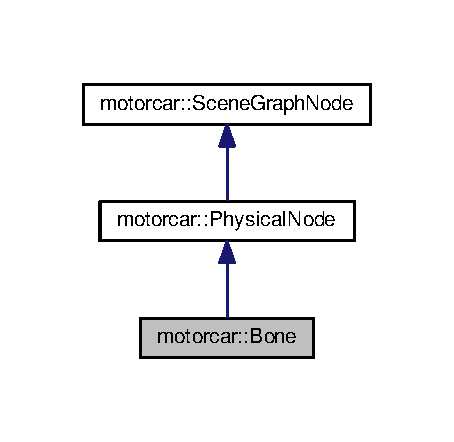
\includegraphics[width=218pt]{classmotorcar_1_1Bone__inherit__graph}
\end{center}
\end{figure}


Collaboration diagram for motorcar\-:\-:Bone\-:
\nopagebreak
\begin{figure}[H]
\begin{center}
\leavevmode
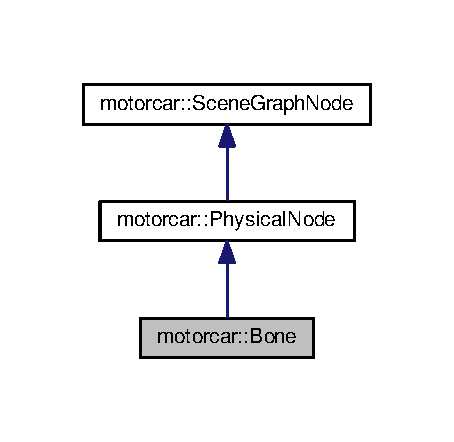
\includegraphics[width=218pt]{classmotorcar_1_1Bone__coll__graph}
\end{center}
\end{figure}
\subsection*{Public Member Functions}
\begin{DoxyCompactItemize}
\item 
\hyperlink{classmotorcar_1_1Bone_adbb164130330e90ec7047495cf45d120}{Bone} (\hyperlink{classmotorcar_1_1PhysicalNode}{Physical\-Node} $\ast$parent, const glm\-::mat4 \&\hyperlink{classmotorcar_1_1SceneGraphNode_ad96e79fdd739ac8223a3128003be391a}{transform}=glm\-::mat4())
\item 
void \hyperlink{classmotorcar_1_1Bone_aaeeac2d80ac8456abbbde7646c5a4c31}{set\-Position} (const glm\-::vec3 \&position)
\begin{DoxyCompactList}\small\item\em Set the position of the bone in parent space. \end{DoxyCompactList}\item 
void \hyperlink{classmotorcar_1_1Bone_ae08fba5b919675716bbbde34e8a17e83}{set\-Orientation} (const glm\-::mat3 \&orientation)
\begin{DoxyCompactList}\small\item\em Set the orientation of the bone in parent space. \end{DoxyCompactList}\end{DoxyCompactItemize}
\subsection*{Additional Inherited Members}


\subsection{Constructor \& Destructor Documentation}
\hypertarget{classmotorcar_1_1Bone_adbb164130330e90ec7047495cf45d120}{\index{motorcar\-::\-Bone@{motorcar\-::\-Bone}!Bone@{Bone}}
\index{Bone@{Bone}!motorcar::Bone@{motorcar\-::\-Bone}}
\subsubsection[{Bone}]{\setlength{\rightskip}{0pt plus 5cm}motorcar\-::\-Bone\-::\-Bone (
\begin{DoxyParamCaption}
\item[{{\bf motorcar\-::\-Physical\-Node} $\ast$}]{parent, }
\item[{const glm\-::mat4 \&}]{transform = {\ttfamily glm\-:\-:mat4()}}
\end{DoxyParamCaption}
)}}\label{classmotorcar_1_1Bone_adbb164130330e90ec7047495cf45d120}


\subsection{Member Function Documentation}
\hypertarget{classmotorcar_1_1Bone_ae08fba5b919675716bbbde34e8a17e83}{\index{motorcar\-::\-Bone@{motorcar\-::\-Bone}!set\-Orientation@{set\-Orientation}}
\index{set\-Orientation@{set\-Orientation}!motorcar::Bone@{motorcar\-::\-Bone}}
\subsubsection[{set\-Orientation}]{\setlength{\rightskip}{0pt plus 5cm}void Bone\-::set\-Orientation (
\begin{DoxyParamCaption}
\item[{const glm\-::mat3 \&}]{orientation}
\end{DoxyParamCaption}
)}}\label{classmotorcar_1_1Bone_ae08fba5b919675716bbbde34e8a17e83}


Set the orientation of the bone in parent space. 

\hypertarget{classmotorcar_1_1Bone_aaeeac2d80ac8456abbbde7646c5a4c31}{\index{motorcar\-::\-Bone@{motorcar\-::\-Bone}!set\-Position@{set\-Position}}
\index{set\-Position@{set\-Position}!motorcar::Bone@{motorcar\-::\-Bone}}
\subsubsection[{set\-Position}]{\setlength{\rightskip}{0pt plus 5cm}void Bone\-::set\-Position (
\begin{DoxyParamCaption}
\item[{const glm\-::vec3 \&}]{position}
\end{DoxyParamCaption}
)}}\label{classmotorcar_1_1Bone_aaeeac2d80ac8456abbbde7646c5a4c31}


Set the position of the bone in parent space. 



The documentation for this class was generated from the following files\-:\begin{DoxyCompactItemize}
\item 
/home/dave/thesis/motorcar/src/compositor/scenegraph/input/\hyperlink{bone_8h}{bone.\-h}\item 
/home/dave/thesis/motorcar/src/compositor/scenegraph/input/\hyperlink{bone_8cpp}{bone.\-cpp}\end{DoxyCompactItemize}

\hypertarget{classmotorcar_1_1BoneSensor}{\section{motorcar\-:\-:Bone\-Sensor Class Reference}
\label{classmotorcar_1_1BoneSensor}\index{motorcar\-::\-Bone\-Sensor@{motorcar\-::\-Bone\-Sensor}}
}


{\ttfamily \#include $<$bonesensor.\-h$>$}



Inheritance diagram for motorcar\-:\-:Bone\-Sensor\-:
\nopagebreak
\begin{figure}[H]
\begin{center}
\leavevmode
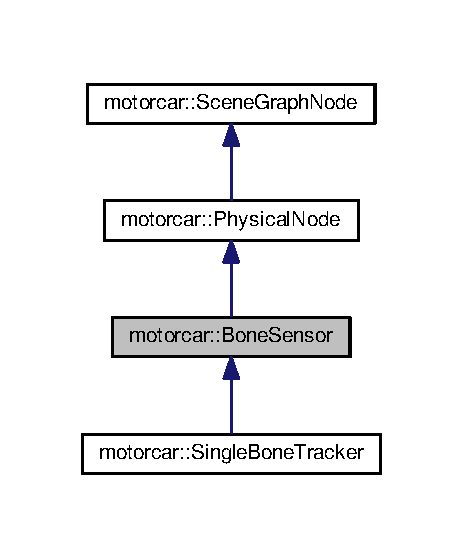
\includegraphics[width=222pt]{classmotorcar_1_1BoneSensor__inherit__graph}
\end{center}
\end{figure}


Collaboration diagram for motorcar\-:\-:Bone\-Sensor\-:
\nopagebreak
\begin{figure}[H]
\begin{center}
\leavevmode
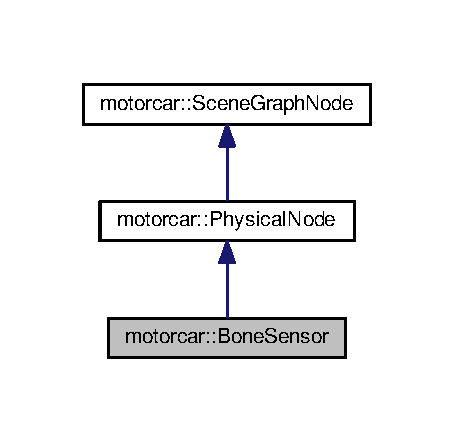
\includegraphics[width=218pt]{classmotorcar_1_1BoneSensor__coll__graph}
\end{center}
\end{figure}
\subsection*{Public Member Functions}
\begin{DoxyCompactItemize}
\item 
\hyperlink{classmotorcar_1_1BoneSensor_a98633120d660896393934a6df827aa69}{Bone\-Sensor} (\hyperlink{classmotorcar_1_1Skeleton}{Skeleton} $\ast$\hyperlink{classmotorcar_1_1BoneSensor_a71f19e3ae5fac133a9f359c5ba4cef00}{skeleton}, \hyperlink{classmotorcar_1_1PhysicalNode}{Physical\-Node} $\ast$parent, const glm\-::mat4 \&\hyperlink{classmotorcar_1_1SceneGraphNode_ad96e79fdd739ac8223a3128003be391a}{transform}=glm\-::mat4())
\item 
\hyperlink{classmotorcar_1_1Skeleton}{Skeleton} $\ast$ \hyperlink{classmotorcar_1_1BoneSensor_a71f19e3ae5fac133a9f359c5ba4cef00}{skeleton} () const 
\item 
void \hyperlink{classmotorcar_1_1BoneSensor_ae84da9d4a2116e603222b72e43f750fe}{set\-Skeleton} (\hyperlink{classmotorcar_1_1Skeleton}{Skeleton} $\ast$\hyperlink{classmotorcar_1_1BoneSensor_a71f19e3ae5fac133a9f359c5ba4cef00}{skeleton})
\end{DoxyCompactItemize}
\subsection*{Additional Inherited Members}


\subsection{Constructor \& Destructor Documentation}
\hypertarget{classmotorcar_1_1BoneSensor_a98633120d660896393934a6df827aa69}{\index{motorcar\-::\-Bone\-Sensor@{motorcar\-::\-Bone\-Sensor}!Bone\-Sensor@{Bone\-Sensor}}
\index{Bone\-Sensor@{Bone\-Sensor}!motorcar::BoneSensor@{motorcar\-::\-Bone\-Sensor}}
\subsubsection[{Bone\-Sensor}]{\setlength{\rightskip}{0pt plus 5cm}Bone\-Sensor\-::\-Bone\-Sensor (
\begin{DoxyParamCaption}
\item[{{\bf Skeleton} $\ast$}]{skeleton, }
\item[{{\bf Physical\-Node} $\ast$}]{parent, }
\item[{const glm\-::mat4 \&}]{transform = {\ttfamily glm\-:\-:mat4()}}
\end{DoxyParamCaption}
)}}\label{classmotorcar_1_1BoneSensor_a98633120d660896393934a6df827aa69}


\subsection{Member Function Documentation}
\hypertarget{classmotorcar_1_1BoneSensor_ae84da9d4a2116e603222b72e43f750fe}{\index{motorcar\-::\-Bone\-Sensor@{motorcar\-::\-Bone\-Sensor}!set\-Skeleton@{set\-Skeleton}}
\index{set\-Skeleton@{set\-Skeleton}!motorcar::BoneSensor@{motorcar\-::\-Bone\-Sensor}}
\subsubsection[{set\-Skeleton}]{\setlength{\rightskip}{0pt plus 5cm}void Bone\-Sensor\-::set\-Skeleton (
\begin{DoxyParamCaption}
\item[{{\bf Skeleton} $\ast$}]{skeleton}
\end{DoxyParamCaption}
)}}\label{classmotorcar_1_1BoneSensor_ae84da9d4a2116e603222b72e43f750fe}
\hypertarget{classmotorcar_1_1BoneSensor_a71f19e3ae5fac133a9f359c5ba4cef00}{\index{motorcar\-::\-Bone\-Sensor@{motorcar\-::\-Bone\-Sensor}!skeleton@{skeleton}}
\index{skeleton@{skeleton}!motorcar::BoneSensor@{motorcar\-::\-Bone\-Sensor}}
\subsubsection[{skeleton}]{\setlength{\rightskip}{0pt plus 5cm}{\bf Skeleton} $\ast$ Bone\-Sensor\-::skeleton (
\begin{DoxyParamCaption}
{}
\end{DoxyParamCaption}
) const}}\label{classmotorcar_1_1BoneSensor_a71f19e3ae5fac133a9f359c5ba4cef00}


The documentation for this class was generated from the following files\-:\begin{DoxyCompactItemize}
\item 
/home/dave/thesis/motorcar/src/compositor/scenegraph/input/\hyperlink{bonesensor_8h}{bonesensor.\-h}\item 
/home/dave/thesis/motorcar/src/compositor/scenegraph/input/\hyperlink{bonesensor_8cpp}{bonesensor.\-cpp}\end{DoxyCompactItemize}

\hypertarget{classBox}{\section{Box Class Reference}
\label{classBox}\index{Box@{Box}}
}
\subsection*{Public Member Functions}
\begin{DoxyCompactItemize}
\item 
void \hyperlink{classBox_a4a575af97c6df4a6726b110680dbebf4}{draw} (struct \hyperlink{structwindow}{window} $\ast$\hyperlink{structwindow}{window}, std\-::vector$<$ struct \hyperlink{structviewpoint}{viewpoint} $\ast$ $>$ \&viewpoints, uint32\-\_\-t time)
\end{DoxyCompactItemize}
\subsection*{Public Attributes}
\begin{DoxyCompactItemize}
\item 
glm\-::vec3 \hyperlink{classBox_a07840041729d30aa0ad28da68ed0d80a}{size}
\item 
glm\-::mat4 \hyperlink{classBox_a1c4ecc1b7eb6717d29022bdb80506b8b}{transform}
\item 
glm\-::mat4 \hyperlink{classBox_ae8b804e1de0abbf9dacf1429a8ffc523}{grab\-Transform}
\item 
bool \hyperlink{classBox_ab56163a3852271ff21236267bb55e6d5}{is\-Grabbed}
\end{DoxyCompactItemize}


\subsection{Member Function Documentation}
\hypertarget{classBox_a4a575af97c6df4a6726b110680dbebf4}{\index{Box@{Box}!draw@{draw}}
\index{draw@{draw}!Box@{Box}}
\subsubsection[{draw}]{\setlength{\rightskip}{0pt plus 5cm}void Box\-::draw (
\begin{DoxyParamCaption}
\item[{struct {\bf window} $\ast$}]{window, }
\item[{std\-::vector$<$ struct {\bf viewpoint} $\ast$ $>$ \&}]{viewpoints, }
\item[{uint32\-\_\-t}]{time}
\end{DoxyParamCaption}
)}}\label{classBox_a4a575af97c6df4a6726b110680dbebf4}


\subsection{Member Data Documentation}
\hypertarget{classBox_ae8b804e1de0abbf9dacf1429a8ffc523}{\index{Box@{Box}!grab\-Transform@{grab\-Transform}}
\index{grab\-Transform@{grab\-Transform}!Box@{Box}}
\subsubsection[{grab\-Transform}]{\setlength{\rightskip}{0pt plus 5cm}glm\-::mat4 Box\-::grab\-Transform}}\label{classBox_ae8b804e1de0abbf9dacf1429a8ffc523}
\hypertarget{classBox_ab56163a3852271ff21236267bb55e6d5}{\index{Box@{Box}!is\-Grabbed@{is\-Grabbed}}
\index{is\-Grabbed@{is\-Grabbed}!Box@{Box}}
\subsubsection[{is\-Grabbed}]{\setlength{\rightskip}{0pt plus 5cm}bool Box\-::is\-Grabbed}}\label{classBox_ab56163a3852271ff21236267bb55e6d5}
\hypertarget{classBox_a07840041729d30aa0ad28da68ed0d80a}{\index{Box@{Box}!size@{size}}
\index{size@{size}!Box@{Box}}
\subsubsection[{size}]{\setlength{\rightskip}{0pt plus 5cm}glm\-::vec3 Box\-::size}}\label{classBox_a07840041729d30aa0ad28da68ed0d80a}
\hypertarget{classBox_a1c4ecc1b7eb6717d29022bdb80506b8b}{\index{Box@{Box}!transform@{transform}}
\index{transform@{transform}!Box@{Box}}
\subsubsection[{transform}]{\setlength{\rightskip}{0pt plus 5cm}glm\-::mat4 Box\-::transform}}\label{classBox_a1c4ecc1b7eb6717d29022bdb80506b8b}


The documentation for this class was generated from the following file\-:\begin{DoxyCompactItemize}
\item 
/home/dave/thesis/motorcar/src/examples/clients/simple-\/egl/\hyperlink{simple-egl_8cpp}{simple-\/egl.\-cpp}\end{DoxyCompactItemize}

\hypertarget{classmotorcar_1_1Compositor}{\section{motorcar\-:\-:Compositor Class Reference}
\label{classmotorcar_1_1Compositor}\index{motorcar\-::\-Compositor@{motorcar\-::\-Compositor}}
}


{\ttfamily \#include $<$compositor.\-h$>$}



Inheritance diagram for motorcar\-:\-:Compositor\-:
\nopagebreak
\begin{figure}[H]
\begin{center}
\leavevmode
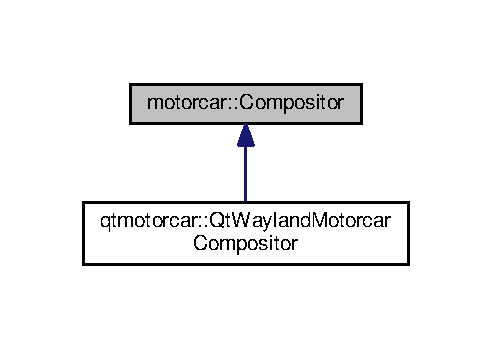
\includegraphics[width=254pt]{classmotorcar_1_1Compositor__inherit__graph}
\end{center}
\end{figure}


Collaboration diagram for motorcar\-:\-:Compositor\-:
\nopagebreak
\begin{figure}[H]
\begin{center}
\leavevmode
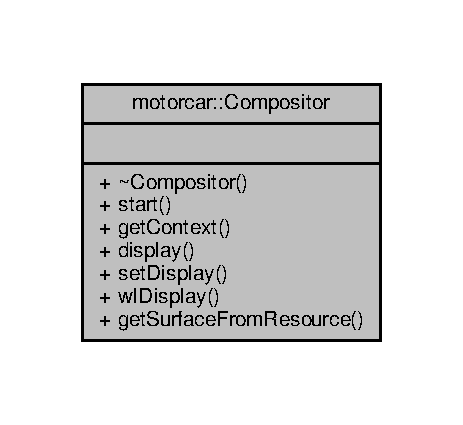
\includegraphics[width=190pt]{classmotorcar_1_1Compositor__coll__graph}
\end{center}
\end{figure}
\subsection*{Public Member Functions}
\begin{DoxyCompactItemize}
\item 
virtual \hyperlink{classmotorcar_1_1Compositor_ab9963bdfdd7deafdaec1a5ebf8f2d97b}{$\sim$\-Compositor} ()
\item 
virtual int \hyperlink{classmotorcar_1_1Compositor_a9d4b703e99386360996087a1100fae52}{start} ()=0
\item 
virtual \hyperlink{classmotorcar_1_1OpenGLContext}{Open\-G\-L\-Context} $\ast$ \hyperlink{classmotorcar_1_1Compositor_afb0a16529f65b5e2ecf8f15524680c57}{get\-Context} ()=0
\item 
\hyperlink{classmotorcar_1_1Display}{Display} $\ast$ \hyperlink{classmotorcar_1_1Compositor_a101830d8941b3d51a57e224950240cfe}{display} () const 
\item 
void \hyperlink{classmotorcar_1_1Compositor_a432fe3ad3e6ff3e22c61b3dc98f719f6}{set\-Display} (\hyperlink{classmotorcar_1_1Display}{Display} $\ast$\hyperlink{classmotorcar_1_1Compositor_a101830d8941b3d51a57e224950240cfe}{display})
\end{DoxyCompactItemize}


\subsection{Constructor \& Destructor Documentation}
\hypertarget{classmotorcar_1_1Compositor_ab9963bdfdd7deafdaec1a5ebf8f2d97b}{\index{motorcar\-::\-Compositor@{motorcar\-::\-Compositor}!$\sim$\-Compositor@{$\sim$\-Compositor}}
\index{$\sim$\-Compositor@{$\sim$\-Compositor}!motorcar::Compositor@{motorcar\-::\-Compositor}}
\subsubsection[{$\sim$\-Compositor}]{\setlength{\rightskip}{0pt plus 5cm}Compositor\-::$\sim$\-Compositor (
\begin{DoxyParamCaption}
{}
\end{DoxyParamCaption}
)\hspace{0.3cm}{\ttfamily [virtual]}}}\label{classmotorcar_1_1Compositor_ab9963bdfdd7deafdaec1a5ebf8f2d97b}


\subsection{Member Function Documentation}
\hypertarget{classmotorcar_1_1Compositor_a101830d8941b3d51a57e224950240cfe}{\index{motorcar\-::\-Compositor@{motorcar\-::\-Compositor}!display@{display}}
\index{display@{display}!motorcar::Compositor@{motorcar\-::\-Compositor}}
\subsubsection[{display}]{\setlength{\rightskip}{0pt plus 5cm}{\bf Display} $\ast$ Compositor\-::display (
\begin{DoxyParamCaption}
{}
\end{DoxyParamCaption}
) const}}\label{classmotorcar_1_1Compositor_a101830d8941b3d51a57e224950240cfe}
\hypertarget{classmotorcar_1_1Compositor_afb0a16529f65b5e2ecf8f15524680c57}{\index{motorcar\-::\-Compositor@{motorcar\-::\-Compositor}!get\-Context@{get\-Context}}
\index{get\-Context@{get\-Context}!motorcar::Compositor@{motorcar\-::\-Compositor}}
\subsubsection[{get\-Context}]{\setlength{\rightskip}{0pt plus 5cm}virtual {\bf Open\-G\-L\-Context}$\ast$ motorcar\-::\-Compositor\-::get\-Context (
\begin{DoxyParamCaption}
{}
\end{DoxyParamCaption}
)\hspace{0.3cm}{\ttfamily [pure virtual]}}}\label{classmotorcar_1_1Compositor_afb0a16529f65b5e2ecf8f15524680c57}


Implemented in \hyperlink{classqtmotorcar_1_1QtWaylandMotorcarCompositor_a1fb6e9d59011be2912bc9cf51496b191}{qtmotorcar\-::\-Qt\-Wayland\-Motorcar\-Compositor}.

\hypertarget{classmotorcar_1_1Compositor_a432fe3ad3e6ff3e22c61b3dc98f719f6}{\index{motorcar\-::\-Compositor@{motorcar\-::\-Compositor}!set\-Display@{set\-Display}}
\index{set\-Display@{set\-Display}!motorcar::Compositor@{motorcar\-::\-Compositor}}
\subsubsection[{set\-Display}]{\setlength{\rightskip}{0pt plus 5cm}void Compositor\-::set\-Display (
\begin{DoxyParamCaption}
\item[{{\bf Display} $\ast$}]{display}
\end{DoxyParamCaption}
)}}\label{classmotorcar_1_1Compositor_a432fe3ad3e6ff3e22c61b3dc98f719f6}
\hypertarget{classmotorcar_1_1Compositor_a9d4b703e99386360996087a1100fae52}{\index{motorcar\-::\-Compositor@{motorcar\-::\-Compositor}!start@{start}}
\index{start@{start}!motorcar::Compositor@{motorcar\-::\-Compositor}}
\subsubsection[{start}]{\setlength{\rightskip}{0pt plus 5cm}virtual int motorcar\-::\-Compositor\-::start (
\begin{DoxyParamCaption}
{}
\end{DoxyParamCaption}
)\hspace{0.3cm}{\ttfamily [pure virtual]}}}\label{classmotorcar_1_1Compositor_a9d4b703e99386360996087a1100fae52}


Implemented in \hyperlink{classqtmotorcar_1_1QtWaylandMotorcarCompositor_a34cd3f4acc535584eb066d3fe32ed9bf}{qtmotorcar\-::\-Qt\-Wayland\-Motorcar\-Compositor}.



The documentation for this class was generated from the following files\-:\begin{DoxyCompactItemize}
\item 
/home/dave/thesis/qtwayland-\/motorcar-\/compositor/motorcar/src/\hyperlink{compositor_8h}{compositor.\-h}\item 
/home/dave/thesis/qtwayland-\/motorcar-\/compositor/motorcar/src/\hyperlink{compositor_8cpp}{compositor.\-cpp}\end{DoxyCompactItemize}

\hypertarget{structdisplay}{\section{display Struct Reference}
\label{structdisplay}\index{display@{display}}
}


Collaboration diagram for display\-:
\nopagebreak
\begin{figure}[H]
\begin{center}
\leavevmode
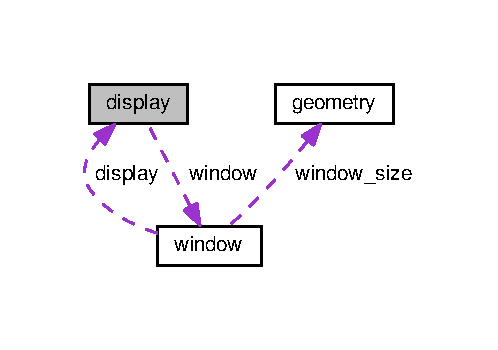
\includegraphics[width=350pt]{structdisplay__coll__graph}
\end{center}
\end{figure}
\subsection*{Public Attributes}
\begin{DoxyCompactItemize}
\item 
struct wl\-\_\-display $\ast$ \hyperlink{structdisplay_aa8faf09631925e9221fd8a0c086ce75a}{display}
\item 
struct wl\-\_\-registry $\ast$ \hyperlink{structdisplay_a925781323f5c8eb84ef2225ed129de4b}{registry}
\item 
struct wl\-\_\-compositor $\ast$ \hyperlink{structdisplay_a41ba32dfde812165dda5b62885000c78}{compositor}
\item 
struct wl\-\_\-shell $\ast$ \hyperlink{structdisplay_a316cfc51e87338b2488233f5d96bd395}{shell}
\item 
struct wl\-\_\-seat $\ast$ \hyperlink{structdisplay_a9dd8fd9967beb6b3767bd93011373bb8}{seat}
\item 
struct wl\-\_\-pointer $\ast$ \hyperlink{structdisplay_acf252129525edb52af1883ed10267754}{pointer}
\item 
struct wl\-\_\-touch $\ast$ \hyperlink{structdisplay_a8adde40dc3f12d1a6967cf424e2284df}{touch}
\item 
struct wl\-\_\-keyboard $\ast$ \hyperlink{structdisplay_a06233e290c4ac294617401b22421691d}{keyboard}
\item 
struct wl\-\_\-shm $\ast$ \hyperlink{structdisplay_abb74b6ec549463cfd4b76f26b81b0309}{shm}
\item 
struct wl\-\_\-cursor\-\_\-theme $\ast$ \hyperlink{structdisplay_a144dd8ac007f779b6eaf1689e225cb35}{cursor\-\_\-theme}
\item 
struct wl\-\_\-cursor $\ast$ \hyperlink{structdisplay_a8cf09ba12cb9ca8cbfa28cf6ca7b668a}{default\-\_\-cursor}
\item 
struct wl\-\_\-surface $\ast$ \hyperlink{structdisplay_a88395d1fffcedd8b841a42e9bd6f7d59}{cursor\-\_\-surface}
\item 
\begin{tabbing}
xx\=xx\=xx\=xx\=xx\=xx\=xx\=xx\=xx\=\kill
struct \{\\
\>EGLDisplay \hyperlink{structdisplay_a8a1cbda15a286e41e89a85f158ce9311}{dpy}\\
\>EGLContext \hyperlink{structdisplay_a3420940a29a710e0e5ebd41ba462cc00}{ctx}\\
\>EGLConfig \hyperlink{structdisplay_a880aef9408b499f5b749541dc6e396c3}{conf}\\
\} \hyperlink{structdisplay_a8b8bc104c19ff228d476a377e572d9c7}{egl}\\

\end{tabbing}\item 
struct \hyperlink{structwindow}{window} $\ast$ \hyperlink{structdisplay_a9974d560bec291487ae2440f897ffc58}{window}
\item 
P\-F\-N\-E\-G\-L\-S\-W\-A\-P\-B\-U\-F\-F\-E\-R\-S\-W\-I\-T\-H\-D\-A\-M\-A\-G\-E\-E\-X\-T\-P\-R\-O\-C \hyperlink{structdisplay_a48c46c118e4765ef06596f6341c8f23f}{swap\-\_\-buffers\-\_\-with\-\_\-damage}
\item 
struct motorcar\-\_\-shell $\ast$ \hyperlink{structdisplay_a0ad2d912a47f21acc312105e1458df68}{motorshell}
\item 
std\-::vector$<$ struct \hyperlink{structviewpoint}{viewpoint} $\ast$ $>$ \hyperlink{structdisplay_ab06917115c7908ddb72c42162d234b72}{viewpoints}
\end{DoxyCompactItemize}


\subsection{Member Data Documentation}
\hypertarget{structdisplay_a41ba32dfde812165dda5b62885000c78}{\index{display@{display}!compositor@{compositor}}
\index{compositor@{compositor}!display@{display}}
\subsubsection[{compositor}]{\setlength{\rightskip}{0pt plus 5cm}struct wl\-\_\-compositor$\ast$ display\-::compositor}}\label{structdisplay_a41ba32dfde812165dda5b62885000c78}
\hypertarget{structdisplay_a880aef9408b499f5b749541dc6e396c3}{\index{display@{display}!conf@{conf}}
\index{conf@{conf}!display@{display}}
\subsubsection[{conf}]{\setlength{\rightskip}{0pt plus 5cm}E\-G\-L\-Config display\-::conf}}\label{structdisplay_a880aef9408b499f5b749541dc6e396c3}
\hypertarget{structdisplay_a3420940a29a710e0e5ebd41ba462cc00}{\index{display@{display}!ctx@{ctx}}
\index{ctx@{ctx}!display@{display}}
\subsubsection[{ctx}]{\setlength{\rightskip}{0pt plus 5cm}E\-G\-L\-Context display\-::ctx}}\label{structdisplay_a3420940a29a710e0e5ebd41ba462cc00}
\hypertarget{structdisplay_a88395d1fffcedd8b841a42e9bd6f7d59}{\index{display@{display}!cursor\-\_\-surface@{cursor\-\_\-surface}}
\index{cursor\-\_\-surface@{cursor\-\_\-surface}!display@{display}}
\subsubsection[{cursor\-\_\-surface}]{\setlength{\rightskip}{0pt plus 5cm}struct wl\-\_\-surface$\ast$ display\-::cursor\-\_\-surface}}\label{structdisplay_a88395d1fffcedd8b841a42e9bd6f7d59}
\hypertarget{structdisplay_a144dd8ac007f779b6eaf1689e225cb35}{\index{display@{display}!cursor\-\_\-theme@{cursor\-\_\-theme}}
\index{cursor\-\_\-theme@{cursor\-\_\-theme}!display@{display}}
\subsubsection[{cursor\-\_\-theme}]{\setlength{\rightskip}{0pt plus 5cm}struct wl\-\_\-cursor\-\_\-theme$\ast$ display\-::cursor\-\_\-theme}}\label{structdisplay_a144dd8ac007f779b6eaf1689e225cb35}
\hypertarget{structdisplay_a8cf09ba12cb9ca8cbfa28cf6ca7b668a}{\index{display@{display}!default\-\_\-cursor@{default\-\_\-cursor}}
\index{default\-\_\-cursor@{default\-\_\-cursor}!display@{display}}
\subsubsection[{default\-\_\-cursor}]{\setlength{\rightskip}{0pt plus 5cm}struct wl\-\_\-cursor$\ast$ display\-::default\-\_\-cursor}}\label{structdisplay_a8cf09ba12cb9ca8cbfa28cf6ca7b668a}
\hypertarget{structdisplay_aa8faf09631925e9221fd8a0c086ce75a}{\index{display@{display}!display@{display}}
\index{display@{display}!display@{display}}
\subsubsection[{display}]{\setlength{\rightskip}{0pt plus 5cm}struct wl\-\_\-display$\ast$ display\-::display}}\label{structdisplay_aa8faf09631925e9221fd8a0c086ce75a}
\hypertarget{structdisplay_a8a1cbda15a286e41e89a85f158ce9311}{\index{display@{display}!dpy@{dpy}}
\index{dpy@{dpy}!display@{display}}
\subsubsection[{dpy}]{\setlength{\rightskip}{0pt plus 5cm}E\-G\-L\-Display display\-::dpy}}\label{structdisplay_a8a1cbda15a286e41e89a85f158ce9311}
\hypertarget{structdisplay_a8b8bc104c19ff228d476a377e572d9c7}{\index{display@{display}!egl@{egl}}
\index{egl@{egl}!display@{display}}
\subsubsection[{egl}]{\setlength{\rightskip}{0pt plus 5cm}struct \{ ... \}   display\-::egl}}\label{structdisplay_a8b8bc104c19ff228d476a377e572d9c7}
\hypertarget{structdisplay_a06233e290c4ac294617401b22421691d}{\index{display@{display}!keyboard@{keyboard}}
\index{keyboard@{keyboard}!display@{display}}
\subsubsection[{keyboard}]{\setlength{\rightskip}{0pt plus 5cm}struct wl\-\_\-keyboard$\ast$ display\-::keyboard}}\label{structdisplay_a06233e290c4ac294617401b22421691d}
\hypertarget{structdisplay_a0ad2d912a47f21acc312105e1458df68}{\index{display@{display}!motorshell@{motorshell}}
\index{motorshell@{motorshell}!display@{display}}
\subsubsection[{motorshell}]{\setlength{\rightskip}{0pt plus 5cm}struct motorcar\-\_\-shell$\ast$ display\-::motorshell}}\label{structdisplay_a0ad2d912a47f21acc312105e1458df68}
\hypertarget{structdisplay_acf252129525edb52af1883ed10267754}{\index{display@{display}!pointer@{pointer}}
\index{pointer@{pointer}!display@{display}}
\subsubsection[{pointer}]{\setlength{\rightskip}{0pt plus 5cm}struct wl\-\_\-pointer$\ast$ display\-::pointer}}\label{structdisplay_acf252129525edb52af1883ed10267754}
\hypertarget{structdisplay_a925781323f5c8eb84ef2225ed129de4b}{\index{display@{display}!registry@{registry}}
\index{registry@{registry}!display@{display}}
\subsubsection[{registry}]{\setlength{\rightskip}{0pt plus 5cm}struct wl\-\_\-registry$\ast$ display\-::registry}}\label{structdisplay_a925781323f5c8eb84ef2225ed129de4b}
\hypertarget{structdisplay_a9dd8fd9967beb6b3767bd93011373bb8}{\index{display@{display}!seat@{seat}}
\index{seat@{seat}!display@{display}}
\subsubsection[{seat}]{\setlength{\rightskip}{0pt plus 5cm}struct wl\-\_\-seat$\ast$ display\-::seat}}\label{structdisplay_a9dd8fd9967beb6b3767bd93011373bb8}
\hypertarget{structdisplay_a316cfc51e87338b2488233f5d96bd395}{\index{display@{display}!shell@{shell}}
\index{shell@{shell}!display@{display}}
\subsubsection[{shell}]{\setlength{\rightskip}{0pt plus 5cm}struct wl\-\_\-shell$\ast$ display\-::shell}}\label{structdisplay_a316cfc51e87338b2488233f5d96bd395}
\hypertarget{structdisplay_abb74b6ec549463cfd4b76f26b81b0309}{\index{display@{display}!shm@{shm}}
\index{shm@{shm}!display@{display}}
\subsubsection[{shm}]{\setlength{\rightskip}{0pt plus 5cm}struct wl\-\_\-shm$\ast$ display\-::shm}}\label{structdisplay_abb74b6ec549463cfd4b76f26b81b0309}
\hypertarget{structdisplay_a48c46c118e4765ef06596f6341c8f23f}{\index{display@{display}!swap\-\_\-buffers\-\_\-with\-\_\-damage@{swap\-\_\-buffers\-\_\-with\-\_\-damage}}
\index{swap\-\_\-buffers\-\_\-with\-\_\-damage@{swap\-\_\-buffers\-\_\-with\-\_\-damage}!display@{display}}
\subsubsection[{swap\-\_\-buffers\-\_\-with\-\_\-damage}]{\setlength{\rightskip}{0pt plus 5cm}P\-F\-N\-E\-G\-L\-S\-W\-A\-P\-B\-U\-F\-F\-E\-R\-S\-W\-I\-T\-H\-D\-A\-M\-A\-G\-E\-E\-X\-T\-P\-R\-O\-C display\-::swap\-\_\-buffers\-\_\-with\-\_\-damage}}\label{structdisplay_a48c46c118e4765ef06596f6341c8f23f}
\hypertarget{structdisplay_a8adde40dc3f12d1a6967cf424e2284df}{\index{display@{display}!touch@{touch}}
\index{touch@{touch}!display@{display}}
\subsubsection[{touch}]{\setlength{\rightskip}{0pt plus 5cm}struct wl\-\_\-touch$\ast$ display\-::touch}}\label{structdisplay_a8adde40dc3f12d1a6967cf424e2284df}
\hypertarget{structdisplay_ab06917115c7908ddb72c42162d234b72}{\index{display@{display}!viewpoints@{viewpoints}}
\index{viewpoints@{viewpoints}!display@{display}}
\subsubsection[{viewpoints}]{\setlength{\rightskip}{0pt plus 5cm}std\-::vector$<$struct {\bf viewpoint} $\ast$$>$ display\-::viewpoints}}\label{structdisplay_ab06917115c7908ddb72c42162d234b72}
\hypertarget{structdisplay_a9974d560bec291487ae2440f897ffc58}{\index{display@{display}!window@{window}}
\index{window@{window}!display@{display}}
\subsubsection[{window}]{\setlength{\rightskip}{0pt plus 5cm}struct {\bf window}$\ast$ display\-::window}}\label{structdisplay_a9974d560bec291487ae2440f897ffc58}


The documentation for this struct was generated from the following file\-:\begin{DoxyCompactItemize}
\item 
/home/dave/thesis/motorcar/src/examples/clients/simple-\/egl/\hyperlink{simple-egl_8cpp}{simple-\/egl.\-cpp}\end{DoxyCompactItemize}

\hypertarget{classmotorcar_1_1Display}{\section{motorcar\-:\-:Display Class Reference}
\label{classmotorcar_1_1Display}\index{motorcar\-::\-Display@{motorcar\-::\-Display}}
}


{\ttfamily \#include $<$display.\-h$>$}



Inheritance diagram for motorcar\-:\-:Display\-:
\nopagebreak
\begin{figure}[H]
\begin{center}
\leavevmode
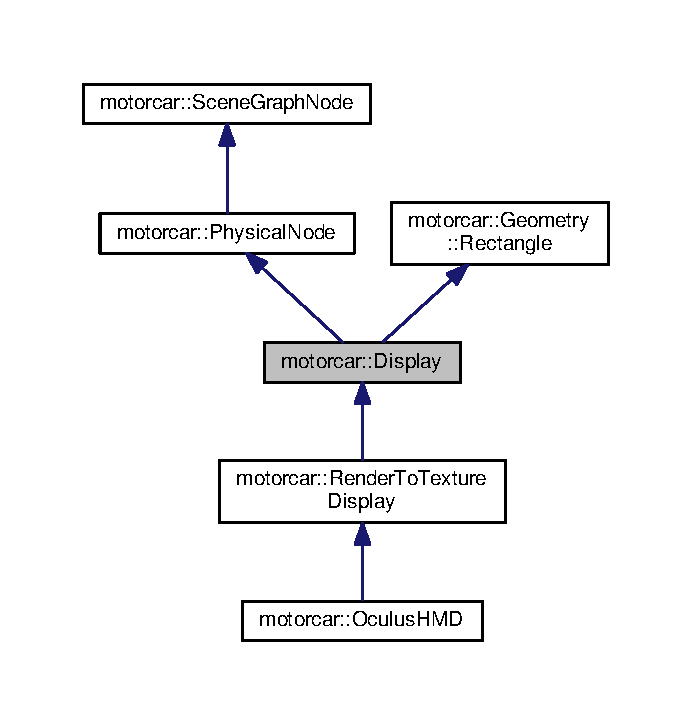
\includegraphics[width=332pt]{classmotorcar_1_1Display__inherit__graph}
\end{center}
\end{figure}


Collaboration diagram for motorcar\-:\-:Display\-:
\nopagebreak
\begin{figure}[H]
\begin{center}
\leavevmode
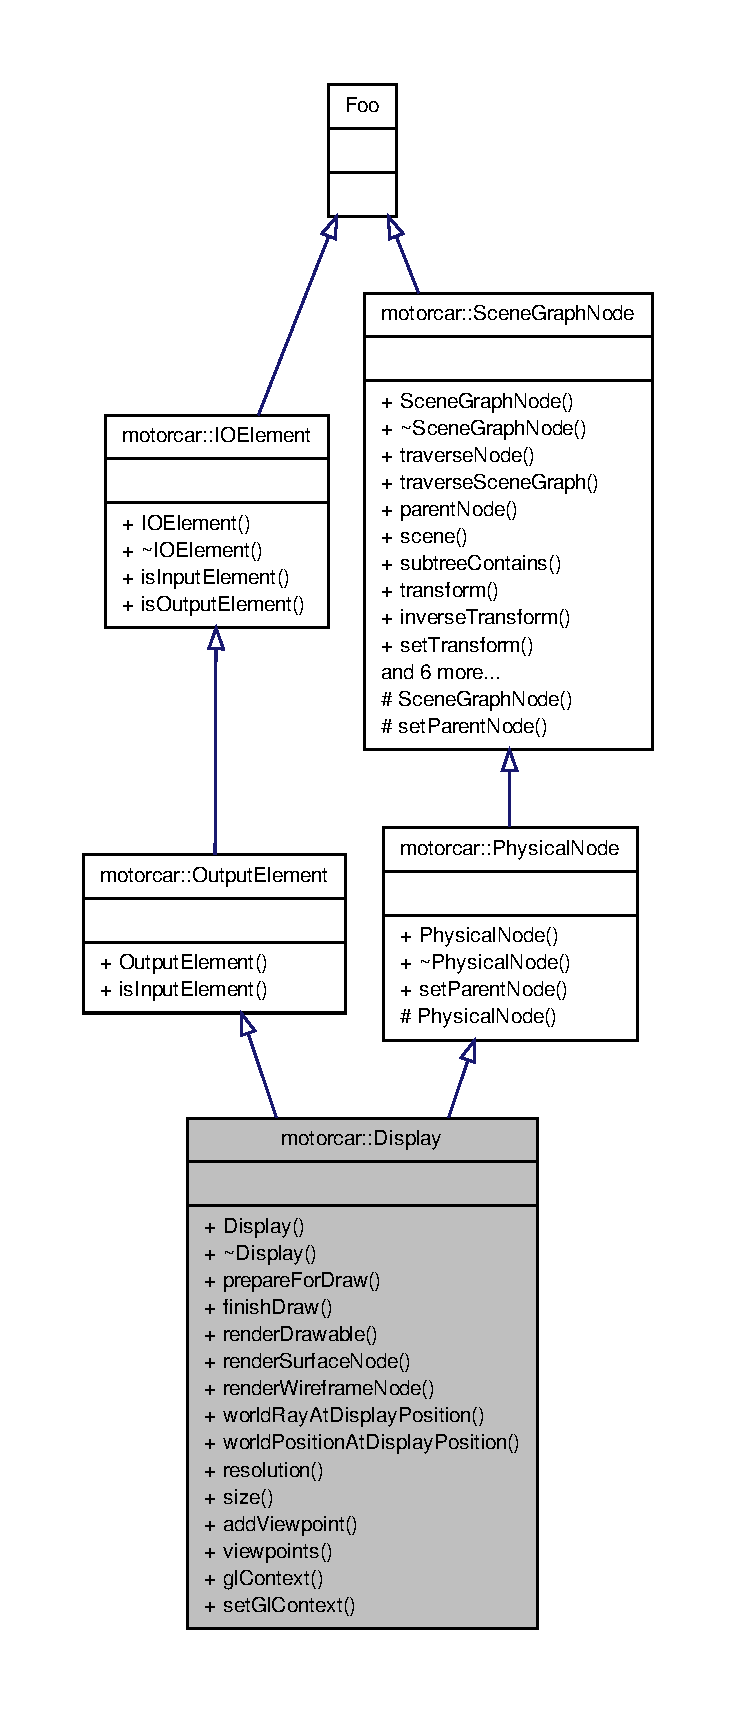
\includegraphics[width=332pt]{classmotorcar_1_1Display__coll__graph}
\end{center}
\end{figure}
\subsection*{Public Member Functions}
\begin{DoxyCompactItemize}
\item 
\hyperlink{classmotorcar_1_1Display_a2f7466d55b00caa97751ee242e0c633c}{Display} (\hyperlink{classmotorcar_1_1OpenGLContext}{Open\-G\-L\-Context} $\ast$\hyperlink{classmotorcar_1_1Display_a884dd0b78dbecee82a33eb6d26a2a403}{gl\-Context}, glm\-::vec2 display\-Dimensions, \hyperlink{classmotorcar_1_1PhysicalNode}{Physical\-Node} $\ast$parent, const glm\-::mat4 \&\hyperlink{classmotorcar_1_1SceneGraphNode_ad96e79fdd739ac8223a3128003be391a}{transform}=glm\-::mat4())
\item 
virtual \hyperlink{classmotorcar_1_1Display_ac2607a6bb236c55547a4223d40d85d1f}{$\sim$\-Display} ()
\item 
virtual void \hyperlink{classmotorcar_1_1Display_a0b26d9162f4f8f0848af408791be631c}{prepare\-For\-Draw} ()
\item 
virtual void \hyperlink{classmotorcar_1_1Display_a162b721d9c039887fc37b6a090ff1074}{finish\-Draw} ()
\item 
virtual \hyperlink{structmotorcar_1_1Geometry_1_1Ray}{Geometry\-::\-Ray} \hyperlink{classmotorcar_1_1Display_a9af842ec6ce47cdc901cb0310b0ef126}{world\-Ray\-At\-Display\-Position} (glm\-::vec2 pixel)
\item 
glm\-::vec3 \hyperlink{classmotorcar_1_1Display_ac3a8d4538e88df5b2bee043504620447}{world\-Position\-At\-Display\-Position} (glm\-::vec2 pixel)
\item 
virtual glm\-::ivec2 \hyperlink{classmotorcar_1_1Display_a58a94b72684d5b8569a9169591f7613e}{size} () override
\item 
virtual glm\-::vec2 \hyperlink{classmotorcar_1_1Display_aea90a885c5f3a124a3581bbeeeb4a425}{dimensions} () const 
\item 
void \hyperlink{classmotorcar_1_1Display_abd961f7f80a84ec143a81a159b07f0e8}{add\-Viewpoint} (\hyperlink{classmotorcar_1_1ViewPoint}{View\-Point} $\ast$v)
\item 
std\-::vector$<$ \hyperlink{classmotorcar_1_1ViewPoint}{View\-Point} $\ast$ $>$ \hyperlink{classmotorcar_1_1Display_acb3f10cbf366d80551f16e224e0bdf73}{viewpoints} () const 
\item 
\hyperlink{classmotorcar_1_1OpenGLContext}{Open\-G\-L\-Context} $\ast$ \hyperlink{classmotorcar_1_1Display_a884dd0b78dbecee82a33eb6d26a2a403}{gl\-Context} () const 
\item 
void \hyperlink{classmotorcar_1_1Display_a487018838d0ecfa96011a5ae5caa2e91}{set\-Gl\-Context} (\hyperlink{classmotorcar_1_1OpenGLContext}{Open\-G\-L\-Context} $\ast$\hyperlink{classmotorcar_1_1Display_a884dd0b78dbecee82a33eb6d26a2a403}{gl\-Context})
\item 
virtual G\-Luint \hyperlink{classmotorcar_1_1Display_a7318ea219f098a3a8b412dcec0745334}{active\-Frame\-Buffer} () const 
\item 
virtual G\-Luint \hyperlink{classmotorcar_1_1Display_a90c69af93ca9d9fff26839fce0e90d53}{depth\-Buffer\-Texture} () const 
\item 
G\-Luint \hyperlink{classmotorcar_1_1Display_ae3d75dd51cb2339bd06905635def61e3}{scratch\-Frame\-Buffer} () const 
\item 
G\-Luint \hyperlink{classmotorcar_1_1Display_a7feeb01b24470cacaee200fa944e24df}{scratch\-Color\-Buffer\-Texture} () const 
\item 
G\-Luint \hyperlink{classmotorcar_1_1Display_ad0b25afba9811f1e85bdf6e4fdc9ff74}{scratch\-Depth\-Buffer\-Texture} () const 
\end{DoxyCompactItemize}
\subsection*{Protected Attributes}
\begin{DoxyCompactItemize}
\item 
G\-Luint \hyperlink{classmotorcar_1_1Display_a23f2535f375102eda1ba2cba2b2a03a4}{m\-\_\-scratch\-Frame\-Buffer}
\item 
G\-Luint \hyperlink{classmotorcar_1_1Display_a8948636502d6498b53fbb644a9064390}{m\-\_\-scratch\-Color\-Buffer\-Texture}
\item 
G\-Luint \hyperlink{classmotorcar_1_1Display_a32e11a89219cf0727cd85b19a30f21a6}{m\-\_\-scratch\-Depth\-Buffer\-Texture}
\end{DoxyCompactItemize}
\subsection*{Additional Inherited Members}


\subsection{Constructor \& Destructor Documentation}
\hypertarget{classmotorcar_1_1Display_a2f7466d55b00caa97751ee242e0c633c}{\index{motorcar\-::\-Display@{motorcar\-::\-Display}!Display@{Display}}
\index{Display@{Display}!motorcar::Display@{motorcar\-::\-Display}}
\subsubsection[{Display}]{\setlength{\rightskip}{0pt plus 5cm}Display\-::\-Display (
\begin{DoxyParamCaption}
\item[{{\bf Open\-G\-L\-Context} $\ast$}]{gl\-Context, }
\item[{glm\-::vec2}]{display\-Dimensions, }
\item[{{\bf Physical\-Node} $\ast$}]{parent, }
\item[{const glm\-::mat4 \&}]{transform = {\ttfamily glm\-:\-:mat4()}}
\end{DoxyParamCaption}
)}}\label{classmotorcar_1_1Display_a2f7466d55b00caa97751ee242e0c633c}
\hypertarget{classmotorcar_1_1Display_ac2607a6bb236c55547a4223d40d85d1f}{\index{motorcar\-::\-Display@{motorcar\-::\-Display}!$\sim$\-Display@{$\sim$\-Display}}
\index{$\sim$\-Display@{$\sim$\-Display}!motorcar::Display@{motorcar\-::\-Display}}
\subsubsection[{$\sim$\-Display}]{\setlength{\rightskip}{0pt plus 5cm}Display\-::$\sim$\-Display (
\begin{DoxyParamCaption}
{}
\end{DoxyParamCaption}
)\hspace{0.3cm}{\ttfamily [virtual]}}}\label{classmotorcar_1_1Display_ac2607a6bb236c55547a4223d40d85d1f}


\subsection{Member Function Documentation}
\hypertarget{classmotorcar_1_1Display_a7318ea219f098a3a8b412dcec0745334}{\index{motorcar\-::\-Display@{motorcar\-::\-Display}!active\-Frame\-Buffer@{active\-Frame\-Buffer}}
\index{active\-Frame\-Buffer@{active\-Frame\-Buffer}!motorcar::Display@{motorcar\-::\-Display}}
\subsubsection[{active\-Frame\-Buffer}]{\setlength{\rightskip}{0pt plus 5cm}virtual G\-Luint motorcar\-::\-Display\-::active\-Frame\-Buffer (
\begin{DoxyParamCaption}
{}
\end{DoxyParamCaption}
) const\hspace{0.3cm}{\ttfamily [inline]}, {\ttfamily [virtual]}}}\label{classmotorcar_1_1Display_a7318ea219f098a3a8b412dcec0745334}


Reimplemented in \hyperlink{classmotorcar_1_1RenderToTextureDisplay_a8c928fb82c28d4785c58a1bd321e0ca6}{motorcar\-::\-Render\-To\-Texture\-Display}.

\hypertarget{classmotorcar_1_1Display_abd961f7f80a84ec143a81a159b07f0e8}{\index{motorcar\-::\-Display@{motorcar\-::\-Display}!add\-Viewpoint@{add\-Viewpoint}}
\index{add\-Viewpoint@{add\-Viewpoint}!motorcar::Display@{motorcar\-::\-Display}}
\subsubsection[{add\-Viewpoint}]{\setlength{\rightskip}{0pt plus 5cm}void Display\-::add\-Viewpoint (
\begin{DoxyParamCaption}
\item[{{\bf View\-Point} $\ast$}]{v}
\end{DoxyParamCaption}
)}}\label{classmotorcar_1_1Display_abd961f7f80a84ec143a81a159b07f0e8}
\hypertarget{classmotorcar_1_1Display_a90c69af93ca9d9fff26839fce0e90d53}{\index{motorcar\-::\-Display@{motorcar\-::\-Display}!depth\-Buffer\-Texture@{depth\-Buffer\-Texture}}
\index{depth\-Buffer\-Texture@{depth\-Buffer\-Texture}!motorcar::Display@{motorcar\-::\-Display}}
\subsubsection[{depth\-Buffer\-Texture}]{\setlength{\rightskip}{0pt plus 5cm}virtual G\-Luint motorcar\-::\-Display\-::depth\-Buffer\-Texture (
\begin{DoxyParamCaption}
{}
\end{DoxyParamCaption}
) const\hspace{0.3cm}{\ttfamily [inline]}, {\ttfamily [virtual]}}}\label{classmotorcar_1_1Display_a90c69af93ca9d9fff26839fce0e90d53}


Reimplemented in \hyperlink{classmotorcar_1_1RenderToTextureDisplay_a4dca5858105e2ee493ef0c49e62c37d4}{motorcar\-::\-Render\-To\-Texture\-Display}.

\hypertarget{classmotorcar_1_1Display_aea90a885c5f3a124a3581bbeeeb4a425}{\index{motorcar\-::\-Display@{motorcar\-::\-Display}!dimensions@{dimensions}}
\index{dimensions@{dimensions}!motorcar::Display@{motorcar\-::\-Display}}
\subsubsection[{dimensions}]{\setlength{\rightskip}{0pt plus 5cm}glm\-::vec2 Display\-::dimensions (
\begin{DoxyParamCaption}
{}
\end{DoxyParamCaption}
) const\hspace{0.3cm}{\ttfamily [virtual]}}}\label{classmotorcar_1_1Display_aea90a885c5f3a124a3581bbeeeb4a425}


Reimplemented in \hyperlink{classmotorcar_1_1RenderToTextureDisplay_a0ede4d9139786227f2c5d87bbbb9dcfa}{motorcar\-::\-Render\-To\-Texture\-Display}.

\hypertarget{classmotorcar_1_1Display_a162b721d9c039887fc37b6a090ff1074}{\index{motorcar\-::\-Display@{motorcar\-::\-Display}!finish\-Draw@{finish\-Draw}}
\index{finish\-Draw@{finish\-Draw}!motorcar::Display@{motorcar\-::\-Display}}
\subsubsection[{finish\-Draw}]{\setlength{\rightskip}{0pt plus 5cm}virtual void motorcar\-::\-Display\-::finish\-Draw (
\begin{DoxyParamCaption}
{}
\end{DoxyParamCaption}
)\hspace{0.3cm}{\ttfamily [inline]}, {\ttfamily [virtual]}}}\label{classmotorcar_1_1Display_a162b721d9c039887fc37b6a090ff1074}


Reimplemented in \hyperlink{classmotorcar_1_1RenderToTextureDisplay_a5a312b98ac49013155797e814e6cf69e}{motorcar\-::\-Render\-To\-Texture\-Display}.

\hypertarget{classmotorcar_1_1Display_a884dd0b78dbecee82a33eb6d26a2a403}{\index{motorcar\-::\-Display@{motorcar\-::\-Display}!gl\-Context@{gl\-Context}}
\index{gl\-Context@{gl\-Context}!motorcar::Display@{motorcar\-::\-Display}}
\subsubsection[{gl\-Context}]{\setlength{\rightskip}{0pt plus 5cm}{\bf Open\-G\-L\-Context} $\ast$ Display\-::gl\-Context (
\begin{DoxyParamCaption}
{}
\end{DoxyParamCaption}
) const}}\label{classmotorcar_1_1Display_a884dd0b78dbecee82a33eb6d26a2a403}
\hypertarget{classmotorcar_1_1Display_a0b26d9162f4f8f0848af408791be631c}{\index{motorcar\-::\-Display@{motorcar\-::\-Display}!prepare\-For\-Draw@{prepare\-For\-Draw}}
\index{prepare\-For\-Draw@{prepare\-For\-Draw}!motorcar::Display@{motorcar\-::\-Display}}
\subsubsection[{prepare\-For\-Draw}]{\setlength{\rightskip}{0pt plus 5cm}void Display\-::prepare\-For\-Draw (
\begin{DoxyParamCaption}
{}
\end{DoxyParamCaption}
)\hspace{0.3cm}{\ttfamily [virtual]}}}\label{classmotorcar_1_1Display_a0b26d9162f4f8f0848af408791be631c}


Reimplemented in \hyperlink{classmotorcar_1_1OculusHMD_ae9834ea50d728809532b7a48f7ed1738}{motorcar\-::\-Oculus\-H\-M\-D}, and \hyperlink{classmotorcar_1_1RenderToTextureDisplay_abdf6861fe69ada64fafd0a7713391bed}{motorcar\-::\-Render\-To\-Texture\-Display}.

\hypertarget{classmotorcar_1_1Display_a7feeb01b24470cacaee200fa944e24df}{\index{motorcar\-::\-Display@{motorcar\-::\-Display}!scratch\-Color\-Buffer\-Texture@{scratch\-Color\-Buffer\-Texture}}
\index{scratch\-Color\-Buffer\-Texture@{scratch\-Color\-Buffer\-Texture}!motorcar::Display@{motorcar\-::\-Display}}
\subsubsection[{scratch\-Color\-Buffer\-Texture}]{\setlength{\rightskip}{0pt plus 5cm}G\-Luint Display\-::scratch\-Color\-Buffer\-Texture (
\begin{DoxyParamCaption}
{}
\end{DoxyParamCaption}
) const}}\label{classmotorcar_1_1Display_a7feeb01b24470cacaee200fa944e24df}
\hypertarget{classmotorcar_1_1Display_ad0b25afba9811f1e85bdf6e4fdc9ff74}{\index{motorcar\-::\-Display@{motorcar\-::\-Display}!scratch\-Depth\-Buffer\-Texture@{scratch\-Depth\-Buffer\-Texture}}
\index{scratch\-Depth\-Buffer\-Texture@{scratch\-Depth\-Buffer\-Texture}!motorcar::Display@{motorcar\-::\-Display}}
\subsubsection[{scratch\-Depth\-Buffer\-Texture}]{\setlength{\rightskip}{0pt plus 5cm}G\-Luint Display\-::scratch\-Depth\-Buffer\-Texture (
\begin{DoxyParamCaption}
{}
\end{DoxyParamCaption}
) const}}\label{classmotorcar_1_1Display_ad0b25afba9811f1e85bdf6e4fdc9ff74}
\hypertarget{classmotorcar_1_1Display_ae3d75dd51cb2339bd06905635def61e3}{\index{motorcar\-::\-Display@{motorcar\-::\-Display}!scratch\-Frame\-Buffer@{scratch\-Frame\-Buffer}}
\index{scratch\-Frame\-Buffer@{scratch\-Frame\-Buffer}!motorcar::Display@{motorcar\-::\-Display}}
\subsubsection[{scratch\-Frame\-Buffer}]{\setlength{\rightskip}{0pt plus 5cm}G\-Luint Display\-::scratch\-Frame\-Buffer (
\begin{DoxyParamCaption}
{}
\end{DoxyParamCaption}
) const}}\label{classmotorcar_1_1Display_ae3d75dd51cb2339bd06905635def61e3}
\hypertarget{classmotorcar_1_1Display_a487018838d0ecfa96011a5ae5caa2e91}{\index{motorcar\-::\-Display@{motorcar\-::\-Display}!set\-Gl\-Context@{set\-Gl\-Context}}
\index{set\-Gl\-Context@{set\-Gl\-Context}!motorcar::Display@{motorcar\-::\-Display}}
\subsubsection[{set\-Gl\-Context}]{\setlength{\rightskip}{0pt plus 5cm}void Display\-::set\-Gl\-Context (
\begin{DoxyParamCaption}
\item[{{\bf Open\-G\-L\-Context} $\ast$}]{gl\-Context}
\end{DoxyParamCaption}
)}}\label{classmotorcar_1_1Display_a487018838d0ecfa96011a5ae5caa2e91}
\hypertarget{classmotorcar_1_1Display_a58a94b72684d5b8569a9169591f7613e}{\index{motorcar\-::\-Display@{motorcar\-::\-Display}!size@{size}}
\index{size@{size}!motorcar::Display@{motorcar\-::\-Display}}
\subsubsection[{size}]{\setlength{\rightskip}{0pt plus 5cm}glm\-::ivec2 Display\-::size (
\begin{DoxyParamCaption}
{}
\end{DoxyParamCaption}
)\hspace{0.3cm}{\ttfamily [override]}, {\ttfamily [virtual]}}}\label{classmotorcar_1_1Display_a58a94b72684d5b8569a9169591f7613e}


Reimplemented from \hyperlink{structmotorcar_1_1Geometry_1_1Rectangle_aef0385032dd32c2b2c762c08f1bfacf6}{motorcar\-::\-Geometry\-::\-Rectangle}.



Reimplemented in \hyperlink{classmotorcar_1_1RenderToTextureDisplay_a2e10611cf3fd629a4d962988642ad5b2}{motorcar\-::\-Render\-To\-Texture\-Display}.

\hypertarget{classmotorcar_1_1Display_acb3f10cbf366d80551f16e224e0bdf73}{\index{motorcar\-::\-Display@{motorcar\-::\-Display}!viewpoints@{viewpoints}}
\index{viewpoints@{viewpoints}!motorcar::Display@{motorcar\-::\-Display}}
\subsubsection[{viewpoints}]{\setlength{\rightskip}{0pt plus 5cm}std\-::vector$<$ {\bf View\-Point} $\ast$ $>$ Display\-::viewpoints (
\begin{DoxyParamCaption}
{}
\end{DoxyParamCaption}
) const}}\label{classmotorcar_1_1Display_acb3f10cbf366d80551f16e224e0bdf73}
\hypertarget{classmotorcar_1_1Display_ac3a8d4538e88df5b2bee043504620447}{\index{motorcar\-::\-Display@{motorcar\-::\-Display}!world\-Position\-At\-Display\-Position@{world\-Position\-At\-Display\-Position}}
\index{world\-Position\-At\-Display\-Position@{world\-Position\-At\-Display\-Position}!motorcar::Display@{motorcar\-::\-Display}}
\subsubsection[{world\-Position\-At\-Display\-Position}]{\setlength{\rightskip}{0pt plus 5cm}glm\-::vec3 Display\-::world\-Position\-At\-Display\-Position (
\begin{DoxyParamCaption}
\item[{glm\-::vec2}]{pixel}
\end{DoxyParamCaption}
)}}\label{classmotorcar_1_1Display_ac3a8d4538e88df5b2bee043504620447}
\hypertarget{classmotorcar_1_1Display_a9af842ec6ce47cdc901cb0310b0ef126}{\index{motorcar\-::\-Display@{motorcar\-::\-Display}!world\-Ray\-At\-Display\-Position@{world\-Ray\-At\-Display\-Position}}
\index{world\-Ray\-At\-Display\-Position@{world\-Ray\-At\-Display\-Position}!motorcar::Display@{motorcar\-::\-Display}}
\subsubsection[{world\-Ray\-At\-Display\-Position}]{\setlength{\rightskip}{0pt plus 5cm}{\bf Geometry\-::\-Ray} Display\-::world\-Ray\-At\-Display\-Position (
\begin{DoxyParamCaption}
\item[{glm\-::vec2}]{pixel}
\end{DoxyParamCaption}
)\hspace{0.3cm}{\ttfamily [virtual]}}}\label{classmotorcar_1_1Display_a9af842ec6ce47cdc901cb0310b0ef126}


\subsection{Member Data Documentation}
\hypertarget{classmotorcar_1_1Display_a8948636502d6498b53fbb644a9064390}{\index{motorcar\-::\-Display@{motorcar\-::\-Display}!m\-\_\-scratch\-Color\-Buffer\-Texture@{m\-\_\-scratch\-Color\-Buffer\-Texture}}
\index{m\-\_\-scratch\-Color\-Buffer\-Texture@{m\-\_\-scratch\-Color\-Buffer\-Texture}!motorcar::Display@{motorcar\-::\-Display}}
\subsubsection[{m\-\_\-scratch\-Color\-Buffer\-Texture}]{\setlength{\rightskip}{0pt plus 5cm}G\-Luint motorcar\-::\-Display\-::m\-\_\-scratch\-Color\-Buffer\-Texture\hspace{0.3cm}{\ttfamily [protected]}}}\label{classmotorcar_1_1Display_a8948636502d6498b53fbb644a9064390}
\hypertarget{classmotorcar_1_1Display_a32e11a89219cf0727cd85b19a30f21a6}{\index{motorcar\-::\-Display@{motorcar\-::\-Display}!m\-\_\-scratch\-Depth\-Buffer\-Texture@{m\-\_\-scratch\-Depth\-Buffer\-Texture}}
\index{m\-\_\-scratch\-Depth\-Buffer\-Texture@{m\-\_\-scratch\-Depth\-Buffer\-Texture}!motorcar::Display@{motorcar\-::\-Display}}
\subsubsection[{m\-\_\-scratch\-Depth\-Buffer\-Texture}]{\setlength{\rightskip}{0pt plus 5cm}G\-Luint motorcar\-::\-Display\-::m\-\_\-scratch\-Depth\-Buffer\-Texture\hspace{0.3cm}{\ttfamily [protected]}}}\label{classmotorcar_1_1Display_a32e11a89219cf0727cd85b19a30f21a6}
\hypertarget{classmotorcar_1_1Display_a23f2535f375102eda1ba2cba2b2a03a4}{\index{motorcar\-::\-Display@{motorcar\-::\-Display}!m\-\_\-scratch\-Frame\-Buffer@{m\-\_\-scratch\-Frame\-Buffer}}
\index{m\-\_\-scratch\-Frame\-Buffer@{m\-\_\-scratch\-Frame\-Buffer}!motorcar::Display@{motorcar\-::\-Display}}
\subsubsection[{m\-\_\-scratch\-Frame\-Buffer}]{\setlength{\rightskip}{0pt plus 5cm}G\-Luint motorcar\-::\-Display\-::m\-\_\-scratch\-Frame\-Buffer\hspace{0.3cm}{\ttfamily [protected]}}}\label{classmotorcar_1_1Display_a23f2535f375102eda1ba2cba2b2a03a4}


The documentation for this class was generated from the following files\-:\begin{DoxyCompactItemize}
\item 
/media/dave/e89b5eb4-\/4b10-\/4edf-\/8ad5-\/0d046a46b978/dave/thesis/qtwayland-\/motorcar-\/compositor/motorcar/src/scenegraph/output/display/\hyperlink{display_8h}{display.\-h}\item 
/media/dave/e89b5eb4-\/4b10-\/4edf-\/8ad5-\/0d046a46b978/dave/thesis/qtwayland-\/motorcar-\/compositor/motorcar/src/scenegraph/output/display/\hyperlink{display_8cpp}{display.\-cpp}\end{DoxyCompactItemize}

\hypertarget{classmotorcar_1_1DisplayServer}{\section{motorcar\-:\-:Display\-Server Class Reference}
\label{classmotorcar_1_1DisplayServer}\index{motorcar\-::\-Display\-Server@{motorcar\-::\-Display\-Server}}
}


This class handles client connection/disconnection and most of the direct wayland interactions.  




{\ttfamily \#include $<$displayserver.\-h$>$}

\subsection*{Public Member Functions}
\begin{DoxyCompactItemize}
\item 
\hyperlink{classmotorcar_1_1DisplayServer_a4ae1fd9d62afe4c74ce8c048d59bc918}{Display\-Server} ()
\end{DoxyCompactItemize}


\subsection{Detailed Description}
This class handles client connection/disconnection and most of the direct wayland interactions. 

\subsection{Constructor \& Destructor Documentation}
\hypertarget{classmotorcar_1_1DisplayServer_a4ae1fd9d62afe4c74ce8c048d59bc918}{\index{motorcar\-::\-Display\-Server@{motorcar\-::\-Display\-Server}!Display\-Server@{Display\-Server}}
\index{Display\-Server@{Display\-Server}!motorcar::DisplayServer@{motorcar\-::\-Display\-Server}}
\subsubsection[{Display\-Server}]{\setlength{\rightskip}{0pt plus 5cm}Display\-Server\-::\-Display\-Server (
\begin{DoxyParamCaption}
{}
\end{DoxyParamCaption}
)}}\label{classmotorcar_1_1DisplayServer_a4ae1fd9d62afe4c74ce8c048d59bc918}


The documentation for this class was generated from the following files\-:\begin{DoxyCompactItemize}
\item 
/home/dave/thesis/motorcar/src/compositor/\hyperlink{displayserver_8h}{displayserver.\-h}\item 
/home/dave/thesis/motorcar/src/compositor/\hyperlink{displayserver_8cpp}{displayserver.\-cpp}\end{DoxyCompactItemize}

\hypertarget{classmotorcar_1_1Drawable}{\section{motorcar\-:\-:Drawable Class Reference}
\label{classmotorcar_1_1Drawable}\index{motorcar\-::\-Drawable@{motorcar\-::\-Drawable}}
}


{\ttfamily \#include $<$drawable.\-h$>$}



Inheritance diagram for motorcar\-:\-:Drawable\-:
\nopagebreak
\begin{figure}[H]
\begin{center}
\leavevmode
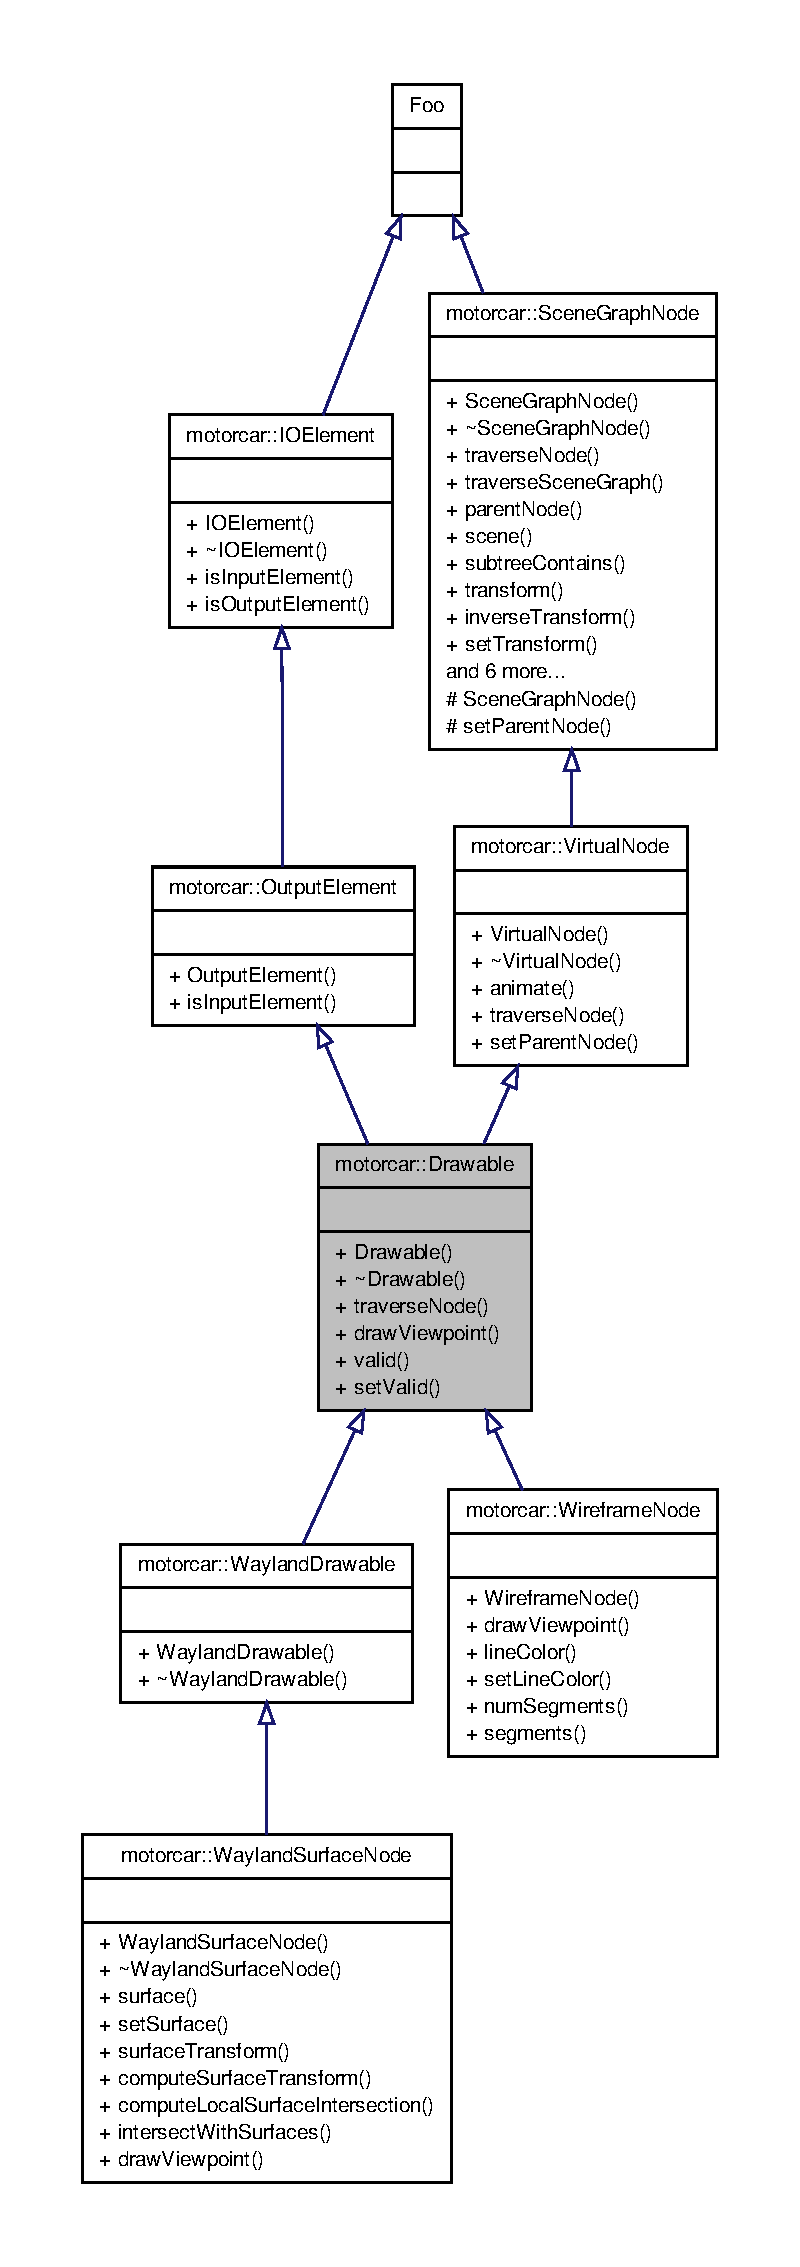
\includegraphics[width=350pt]{classmotorcar_1_1Drawable__inherit__graph}
\end{center}
\end{figure}


Collaboration diagram for motorcar\-:\-:Drawable\-:
\nopagebreak
\begin{figure}[H]
\begin{center}
\leavevmode
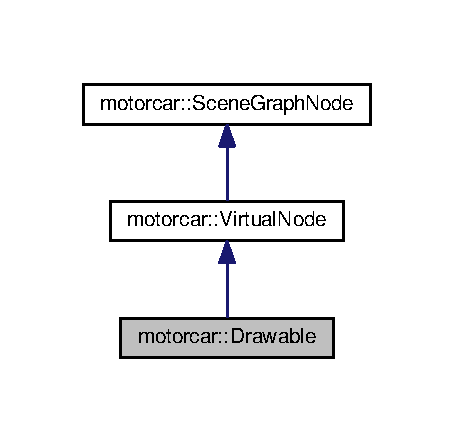
\includegraphics[width=218pt]{classmotorcar_1_1Drawable__coll__graph}
\end{center}
\end{figure}
\subsection*{Public Member Functions}
\begin{DoxyCompactItemize}
\item 
\hyperlink{classmotorcar_1_1Drawable_a48451c25ab7c1e379afec893f4c3d6f3}{Drawable} (\hyperlink{classmotorcar_1_1SceneGraphNode}{Scene\-Graph\-Node} $\ast$parent, const glm\-::mat4 \&\hyperlink{classmotorcar_1_1SceneGraphNode_ad96e79fdd739ac8223a3128003be391a}{transform}=glm\-::mat4())
\item 
virtual \hyperlink{classmotorcar_1_1Drawable_ab638464364b93a00bdeacc64cc85ba41}{$\sim$\-Drawable} ()
\item 
virtual void \hyperlink{classmotorcar_1_1Drawable_a8d0afa524298ae7f4ced15f6a80f253d}{draw} (\hyperlink{classmotorcar_1_1Scene}{Scene} $\ast$\hyperlink{classmotorcar_1_1SceneGraphNode_aa14e637ed4ae98f77e28941a4b5cfdd8}{scene}, \hyperlink{classmotorcar_1_1Display}{Display} $\ast$\hyperlink{structdisplay}{display})=0
\begin{DoxyCompactList}\small\item\em Draw this node for the current display. \end{DoxyCompactList}\item 
virtual void \hyperlink{classmotorcar_1_1Drawable_a8dce7e2370f9fdc5394cf661effc865a}{handle\-Frame\-Draw} (\hyperlink{classmotorcar_1_1Scene}{Scene} $\ast$\hyperlink{classmotorcar_1_1SceneGraphNode_aa14e637ed4ae98f77e28941a4b5cfdd8}{scene}) override
\begin{DoxyCompactList}\small\item\em Gets the active display from the scene and calls draw on it. \end{DoxyCompactList}\item 
bool \hyperlink{classmotorcar_1_1Drawable_ae76952e4af87589dbb7a4c9f17f2fdfa}{visible} () const 
\item 
void \hyperlink{classmotorcar_1_1Drawable_a3aa8dfd1f526d0cf744313e8e102cea4}{set\-Visible} (bool \hyperlink{classmotorcar_1_1Drawable_ae76952e4af87589dbb7a4c9f17f2fdfa}{visible})
\end{DoxyCompactItemize}
\subsection*{Additional Inherited Members}


\subsection{Constructor \& Destructor Documentation}
\hypertarget{classmotorcar_1_1Drawable_a48451c25ab7c1e379afec893f4c3d6f3}{\index{motorcar\-::\-Drawable@{motorcar\-::\-Drawable}!Drawable@{Drawable}}
\index{Drawable@{Drawable}!motorcar::Drawable@{motorcar\-::\-Drawable}}
\subsubsection[{Drawable}]{\setlength{\rightskip}{0pt plus 5cm}Drawable\-::\-Drawable (
\begin{DoxyParamCaption}
\item[{{\bf Scene\-Graph\-Node} $\ast$}]{parent, }
\item[{const glm\-::mat4 \&}]{transform = {\ttfamily glm\-:\-:mat4()}}
\end{DoxyParamCaption}
)}}\label{classmotorcar_1_1Drawable_a48451c25ab7c1e379afec893f4c3d6f3}
\hypertarget{classmotorcar_1_1Drawable_ab638464364b93a00bdeacc64cc85ba41}{\index{motorcar\-::\-Drawable@{motorcar\-::\-Drawable}!$\sim$\-Drawable@{$\sim$\-Drawable}}
\index{$\sim$\-Drawable@{$\sim$\-Drawable}!motorcar::Drawable@{motorcar\-::\-Drawable}}
\subsubsection[{$\sim$\-Drawable}]{\setlength{\rightskip}{0pt plus 5cm}virtual motorcar\-::\-Drawable\-::$\sim$\-Drawable (
\begin{DoxyParamCaption}
{}
\end{DoxyParamCaption}
)\hspace{0.3cm}{\ttfamily [inline]}, {\ttfamily [virtual]}}}\label{classmotorcar_1_1Drawable_ab638464364b93a00bdeacc64cc85ba41}


\subsection{Member Function Documentation}
\hypertarget{classmotorcar_1_1Drawable_a8d0afa524298ae7f4ced15f6a80f253d}{\index{motorcar\-::\-Drawable@{motorcar\-::\-Drawable}!draw@{draw}}
\index{draw@{draw}!motorcar::Drawable@{motorcar\-::\-Drawable}}
\subsubsection[{draw}]{\setlength{\rightskip}{0pt plus 5cm}virtual void motorcar\-::\-Drawable\-::draw (
\begin{DoxyParamCaption}
\item[{{\bf Scene} $\ast$}]{scene, }
\item[{{\bf Display} $\ast$}]{display}
\end{DoxyParamCaption}
)\hspace{0.3cm}{\ttfamily [pure virtual]}}}\label{classmotorcar_1_1Drawable_a8d0afa524298ae7f4ced15f6a80f253d}


Draw this node for the current display. 



Implemented in \hyperlink{classmotorcar_1_1WaylandSurfaceNode_a1afe3178777574dd1b3c66d7d19d871b}{motorcar\-::\-Wayland\-Surface\-Node}, \hyperlink{classmotorcar_1_1SoftKineticDepthCamera_a2752b6bf323e019a4cec43b61d78bcff}{motorcar\-::\-Soft\-Kinetic\-Depth\-Camera}, \hyperlink{classmotorcar_1_1DepthCompositedSurfaceNode_a2108d586ac8641beec9f6d048e3ea562}{motorcar\-::\-Depth\-Composited\-Surface\-Node}, and \hyperlink{classmotorcar_1_1WireframeNode_a8be77469b6c99cfb05c2096b6d064c2e}{motorcar\-::\-Wireframe\-Node}.

\hypertarget{classmotorcar_1_1Drawable_a8dce7e2370f9fdc5394cf661effc865a}{\index{motorcar\-::\-Drawable@{motorcar\-::\-Drawable}!handle\-Frame\-Draw@{handle\-Frame\-Draw}}
\index{handle\-Frame\-Draw@{handle\-Frame\-Draw}!motorcar::Drawable@{motorcar\-::\-Drawable}}
\subsubsection[{handle\-Frame\-Draw}]{\setlength{\rightskip}{0pt plus 5cm}void Drawable\-::handle\-Frame\-Draw (
\begin{DoxyParamCaption}
\item[{{\bf Scene} $\ast$}]{scene}
\end{DoxyParamCaption}
)\hspace{0.3cm}{\ttfamily [override]}, {\ttfamily [virtual]}}}\label{classmotorcar_1_1Drawable_a8dce7e2370f9fdc5394cf661effc865a}


Gets the active display from the scene and calls draw on it. 



Reimplemented from \hyperlink{classmotorcar_1_1SceneGraphNode_a06f85abeee71ebe2b21ca9d6d20d7e67}{motorcar\-::\-Scene\-Graph\-Node}.

\hypertarget{classmotorcar_1_1Drawable_a3aa8dfd1f526d0cf744313e8e102cea4}{\index{motorcar\-::\-Drawable@{motorcar\-::\-Drawable}!set\-Visible@{set\-Visible}}
\index{set\-Visible@{set\-Visible}!motorcar::Drawable@{motorcar\-::\-Drawable}}
\subsubsection[{set\-Visible}]{\setlength{\rightskip}{0pt plus 5cm}void Drawable\-::set\-Visible (
\begin{DoxyParamCaption}
\item[{bool}]{visible}
\end{DoxyParamCaption}
)}}\label{classmotorcar_1_1Drawable_a3aa8dfd1f526d0cf744313e8e102cea4}
\hypertarget{classmotorcar_1_1Drawable_ae76952e4af87589dbb7a4c9f17f2fdfa}{\index{motorcar\-::\-Drawable@{motorcar\-::\-Drawable}!visible@{visible}}
\index{visible@{visible}!motorcar::Drawable@{motorcar\-::\-Drawable}}
\subsubsection[{visible}]{\setlength{\rightskip}{0pt plus 5cm}bool Drawable\-::visible (
\begin{DoxyParamCaption}
{}
\end{DoxyParamCaption}
) const}}\label{classmotorcar_1_1Drawable_ae76952e4af87589dbb7a4c9f17f2fdfa}


The documentation for this class was generated from the following files\-:\begin{DoxyCompactItemize}
\item 
/media/dave/e89b5eb4-\/4b10-\/4edf-\/8ad5-\/0d046a46b978/dave/thesis/qtwayland-\/motorcar-\/compositor/motorcar/src/scenegraph/output/\hyperlink{drawable_8h}{drawable.\-h}\item 
/media/dave/e89b5eb4-\/4b10-\/4edf-\/8ad5-\/0d046a46b978/dave/thesis/qtwayland-\/motorcar-\/compositor/motorcar/src/scenegraph/output/\hyperlink{drawable_8cpp}{drawable.\-cpp}\end{DoxyCompactItemize}

\hypertarget{classmotorcar_1_1Event}{\section{motorcar\-:\-:Event Class Reference}
\label{classmotorcar_1_1Event}\index{motorcar\-::\-Event@{motorcar\-::\-Event}}
}


{\ttfamily \#include $<$event.\-h$>$}



Inheritance diagram for motorcar\-:\-:Event\-:
\nopagebreak
\begin{figure}[H]
\begin{center}
\leavevmode
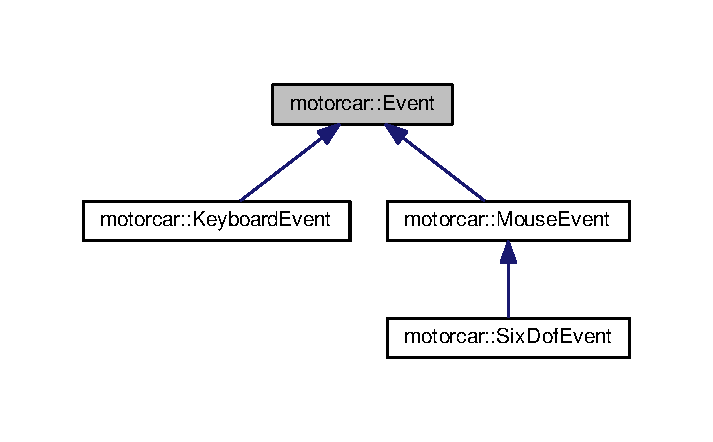
\includegraphics[width=342pt]{classmotorcar_1_1Event__inherit__graph}
\end{center}
\end{figure}
\subsection*{Public Types}
\begin{DoxyCompactItemize}
\item 
enum \hyperlink{classmotorcar_1_1Event_af4f5d9ed7dc2d8a2324fa5b0d32c29b0}{Event\-Type} \{ \hyperlink{classmotorcar_1_1Event_af4f5d9ed7dc2d8a2324fa5b0d32c29b0a03dadb42ea3036c0a8b1bfa6fac4072e}{M\-O\-U\-S\-E}, 
\hyperlink{classmotorcar_1_1Event_af4f5d9ed7dc2d8a2324fa5b0d32c29b0a6a50b4eb2b4d2086997bc94fc075d4c9}{K\-E\-Y\-B\-O\-A\-R\-D}, 
\hyperlink{classmotorcar_1_1Event_af4f5d9ed7dc2d8a2324fa5b0d32c29b0a71e14a650a78d42baa12a22e5cd4ad00}{T\-O\-U\-C\-H}
 \}
\end{DoxyCompactItemize}
\subsection*{Public Member Functions}
\begin{DoxyCompactItemize}
\item 
\hyperlink{classmotorcar_1_1Event_aed0a7622e5b4de79eb9c9115993aebbe}{Event} (\hyperlink{classmotorcar_1_1Seat}{Seat} $\ast$\hyperlink{classmotorcar_1_1Event_a7426828c8402193cac63a7b3fda5a17e}{seat})
\item 
virtual \hyperlink{classmotorcar_1_1Event_a3ff67253553db1d656e32a5e660a3ecb}{$\sim$\-Event} ()
\item 
virtual \hyperlink{classmotorcar_1_1Event_af4f5d9ed7dc2d8a2324fa5b0d32c29b0}{Event\-Type} \hyperlink{classmotorcar_1_1Event_a195195c53c024bc76aa0e550ffe438a6}{type} () const =0
\item 
\hyperlink{classmotorcar_1_1Seat}{Seat} $\ast$ \hyperlink{classmotorcar_1_1Event_a7426828c8402193cac63a7b3fda5a17e}{seat} () const 
\end{DoxyCompactItemize}


\subsection{Member Enumeration Documentation}
\hypertarget{classmotorcar_1_1Event_af4f5d9ed7dc2d8a2324fa5b0d32c29b0}{\index{motorcar\-::\-Event@{motorcar\-::\-Event}!Event\-Type@{Event\-Type}}
\index{Event\-Type@{Event\-Type}!motorcar::Event@{motorcar\-::\-Event}}
\subsubsection[{Event\-Type}]{\setlength{\rightskip}{0pt plus 5cm}enum {\bf motorcar\-::\-Event\-::\-Event\-Type}}}\label{classmotorcar_1_1Event_af4f5d9ed7dc2d8a2324fa5b0d32c29b0}
\begin{Desc}
\item[Enumerator]\par
\begin{description}
\index{M\-O\-U\-S\-E@{M\-O\-U\-S\-E}!motorcar\-::\-Event@{motorcar\-::\-Event}}\index{motorcar\-::\-Event@{motorcar\-::\-Event}!M\-O\-U\-S\-E@{M\-O\-U\-S\-E}}\item[{\em 
\hypertarget{classmotorcar_1_1Event_af4f5d9ed7dc2d8a2324fa5b0d32c29b0a03dadb42ea3036c0a8b1bfa6fac4072e}{M\-O\-U\-S\-E}\label{classmotorcar_1_1Event_af4f5d9ed7dc2d8a2324fa5b0d32c29b0a03dadb42ea3036c0a8b1bfa6fac4072e}
}]\index{K\-E\-Y\-B\-O\-A\-R\-D@{K\-E\-Y\-B\-O\-A\-R\-D}!motorcar\-::\-Event@{motorcar\-::\-Event}}\index{motorcar\-::\-Event@{motorcar\-::\-Event}!K\-E\-Y\-B\-O\-A\-R\-D@{K\-E\-Y\-B\-O\-A\-R\-D}}\item[{\em 
\hypertarget{classmotorcar_1_1Event_af4f5d9ed7dc2d8a2324fa5b0d32c29b0a6a50b4eb2b4d2086997bc94fc075d4c9}{K\-E\-Y\-B\-O\-A\-R\-D}\label{classmotorcar_1_1Event_af4f5d9ed7dc2d8a2324fa5b0d32c29b0a6a50b4eb2b4d2086997bc94fc075d4c9}
}]\index{T\-O\-U\-C\-H@{T\-O\-U\-C\-H}!motorcar\-::\-Event@{motorcar\-::\-Event}}\index{motorcar\-::\-Event@{motorcar\-::\-Event}!T\-O\-U\-C\-H@{T\-O\-U\-C\-H}}\item[{\em 
\hypertarget{classmotorcar_1_1Event_af4f5d9ed7dc2d8a2324fa5b0d32c29b0a71e14a650a78d42baa12a22e5cd4ad00}{T\-O\-U\-C\-H}\label{classmotorcar_1_1Event_af4f5d9ed7dc2d8a2324fa5b0d32c29b0a71e14a650a78d42baa12a22e5cd4ad00}
}]\end{description}
\end{Desc}


\subsection{Constructor \& Destructor Documentation}
\hypertarget{classmotorcar_1_1Event_aed0a7622e5b4de79eb9c9115993aebbe}{\index{motorcar\-::\-Event@{motorcar\-::\-Event}!Event@{Event}}
\index{Event@{Event}!motorcar::Event@{motorcar\-::\-Event}}
\subsubsection[{Event}]{\setlength{\rightskip}{0pt plus 5cm}Event\-::\-Event (
\begin{DoxyParamCaption}
\item[{{\bf Seat} $\ast$}]{seat}
\end{DoxyParamCaption}
)}}\label{classmotorcar_1_1Event_aed0a7622e5b4de79eb9c9115993aebbe}
\hypertarget{classmotorcar_1_1Event_a3ff67253553db1d656e32a5e660a3ecb}{\index{motorcar\-::\-Event@{motorcar\-::\-Event}!$\sim$\-Event@{$\sim$\-Event}}
\index{$\sim$\-Event@{$\sim$\-Event}!motorcar::Event@{motorcar\-::\-Event}}
\subsubsection[{$\sim$\-Event}]{\setlength{\rightskip}{0pt plus 5cm}virtual motorcar\-::\-Event\-::$\sim$\-Event (
\begin{DoxyParamCaption}
{}
\end{DoxyParamCaption}
)\hspace{0.3cm}{\ttfamily [inline]}, {\ttfamily [virtual]}}}\label{classmotorcar_1_1Event_a3ff67253553db1d656e32a5e660a3ecb}


\subsection{Member Function Documentation}
\hypertarget{classmotorcar_1_1Event_a7426828c8402193cac63a7b3fda5a17e}{\index{motorcar\-::\-Event@{motorcar\-::\-Event}!seat@{seat}}
\index{seat@{seat}!motorcar::Event@{motorcar\-::\-Event}}
\subsubsection[{seat}]{\setlength{\rightskip}{0pt plus 5cm}{\bf Seat} $\ast$ Event\-::seat (
\begin{DoxyParamCaption}
{}
\end{DoxyParamCaption}
) const}}\label{classmotorcar_1_1Event_a7426828c8402193cac63a7b3fda5a17e}
\hypertarget{classmotorcar_1_1Event_a195195c53c024bc76aa0e550ffe438a6}{\index{motorcar\-::\-Event@{motorcar\-::\-Event}!type@{type}}
\index{type@{type}!motorcar::Event@{motorcar\-::\-Event}}
\subsubsection[{type}]{\setlength{\rightskip}{0pt plus 5cm}virtual {\bf Event\-Type} motorcar\-::\-Event\-::type (
\begin{DoxyParamCaption}
{}
\end{DoxyParamCaption}
) const\hspace{0.3cm}{\ttfamily [pure virtual]}}}\label{classmotorcar_1_1Event_a195195c53c024bc76aa0e550ffe438a6}


Implemented in \hyperlink{classmotorcar_1_1MouseEvent_afb419c29a7d2fa6dd429eeb3ac0699c5}{motorcar\-::\-Mouse\-Event}, and \hyperlink{classmotorcar_1_1KeyboardEvent_abb35a59eab2d715433ef46868a69df68}{motorcar\-::\-Keyboard\-Event}.



The documentation for this class was generated from the following files\-:\begin{DoxyCompactItemize}
\item 
/media/dave/e89b5eb4-\/4b10-\/4edf-\/8ad5-\/0d046a46b978/dave/thesis/qtwayland-\/motorcar-\/compositor/motorcar/src/events/\hyperlink{event_8h}{event.\-h}\item 
/media/dave/e89b5eb4-\/4b10-\/4edf-\/8ad5-\/0d046a46b978/dave/thesis/qtwayland-\/motorcar-\/compositor/motorcar/src/events/\hyperlink{event_8cpp}{event.\-cpp}\end{DoxyCompactItemize}

\hypertarget{structgeometry}{\section{geometry Struct Reference}
\label{structgeometry}\index{geometry@{geometry}}
}
\subsection*{Public Attributes}
\begin{DoxyCompactItemize}
\item 
int \hyperlink{structgeometry_a854a87ce277335591f06958a2363c3e1}{width}
\item 
int \hyperlink{structgeometry_a6968ae18c72699d1c164399bf0e5cf14}{height}
\end{DoxyCompactItemize}


\subsection{Member Data Documentation}
\hypertarget{structgeometry_a6968ae18c72699d1c164399bf0e5cf14}{\index{geometry@{geometry}!height@{height}}
\index{height@{height}!geometry@{geometry}}
\subsubsection[{height}]{\setlength{\rightskip}{0pt plus 5cm}int geometry\-::height}}\label{structgeometry_a6968ae18c72699d1c164399bf0e5cf14}
\hypertarget{structgeometry_a854a87ce277335591f06958a2363c3e1}{\index{geometry@{geometry}!width@{width}}
\index{width@{width}!geometry@{geometry}}
\subsubsection[{width}]{\setlength{\rightskip}{0pt plus 5cm}int geometry\-::width}}\label{structgeometry_a854a87ce277335591f06958a2363c3e1}


The documentation for this struct was generated from the following file\-:\begin{DoxyCompactItemize}
\item 
/media/dave/e89b5eb4-\/4b10-\/4edf-\/8ad5-\/0d046a46b978/dave/thesis/qtwayland-\/motorcar-\/compositor/motorcar/clients/simple-\/egl/\hyperlink{simple-egl_8c}{simple-\/egl.\-c}\end{DoxyCompactItemize}

\hypertarget{classmotorcar_1_1Geometry}{\section{motorcar\-:\-:Geometry Class Reference}
\label{classmotorcar_1_1Geometry}\index{motorcar\-::\-Geometry@{motorcar\-::\-Geometry}}
}


{\ttfamily \#include $<$geometry.\-h$>$}

\subsection*{Classes}
\begin{DoxyCompactItemize}
\item 
struct \hyperlink{structmotorcar_1_1Geometry_1_1AxisAlignedBox}{Axis\-Aligned\-Box}
\item 
struct \hyperlink{structmotorcar_1_1Geometry_1_1Plane}{Plane}
\item 
struct \hyperlink{structmotorcar_1_1Geometry_1_1Ray}{Ray}
\item 
struct \hyperlink{structmotorcar_1_1Geometry_1_1RaySurfaceIntersection}{Ray\-Surface\-Intersection}
\item 
struct \hyperlink{structmotorcar_1_1Geometry_1_1Rectangle}{Rectangle}
\end{DoxyCompactItemize}
\subsection*{Static Public Member Functions}
\begin{DoxyCompactItemize}
\item 
static void \hyperlink{classmotorcar_1_1Geometry_a35ee70e5dab9981b9f1914eca9580b06}{print\-Matrix} (glm\-::mat4 m)
\item 
static void \hyperlink{classmotorcar_1_1Geometry_a97660333acd464a86c5ab7f5672fb3d2}{print\-Vector} (glm\-::vec3 v)
\end{DoxyCompactItemize}


\subsection{Member Function Documentation}
\hypertarget{classmotorcar_1_1Geometry_a35ee70e5dab9981b9f1914eca9580b06}{\index{motorcar\-::\-Geometry@{motorcar\-::\-Geometry}!print\-Matrix@{print\-Matrix}}
\index{print\-Matrix@{print\-Matrix}!motorcar::Geometry@{motorcar\-::\-Geometry}}
\subsubsection[{print\-Matrix}]{\setlength{\rightskip}{0pt plus 5cm}void Geometry\-::print\-Matrix (
\begin{DoxyParamCaption}
\item[{glm\-::mat4}]{m}
\end{DoxyParamCaption}
)\hspace{0.3cm}{\ttfamily [static]}}}\label{classmotorcar_1_1Geometry_a35ee70e5dab9981b9f1914eca9580b06}
\hypertarget{classmotorcar_1_1Geometry_a97660333acd464a86c5ab7f5672fb3d2}{\index{motorcar\-::\-Geometry@{motorcar\-::\-Geometry}!print\-Vector@{print\-Vector}}
\index{print\-Vector@{print\-Vector}!motorcar::Geometry@{motorcar\-::\-Geometry}}
\subsubsection[{print\-Vector}]{\setlength{\rightskip}{0pt plus 5cm}void Geometry\-::print\-Vector (
\begin{DoxyParamCaption}
\item[{glm\-::vec3}]{v}
\end{DoxyParamCaption}
)\hspace{0.3cm}{\ttfamily [static]}}}\label{classmotorcar_1_1Geometry_a97660333acd464a86c5ab7f5672fb3d2}


The documentation for this class was generated from the following files\-:\begin{DoxyCompactItemize}
\item 
/home/dave/thesis/motorcar/src/compositor/\hyperlink{geometry_8h}{geometry.\-h}\item 
/home/dave/thesis/motorcar/src/compositor/\hyperlink{geometry_8cpp}{geometry.\-cpp}\end{DoxyCompactItemize}

\hypertarget{classGlBufferObject}{\section{Gl\-Buffer\-Object Class Reference}
\label{classGlBufferObject}\index{Gl\-Buffer\-Object@{Gl\-Buffer\-Object}}
}


{\ttfamily \#include $<$G\-L\-S\-L\-Helper.\-h$>$}

\subsection*{Public Member Functions}
\begin{DoxyCompactItemize}
\item 
\hyperlink{classGlBufferObject_a5346228ff9f5b1c806a9d03ece525dbb}{Gl\-Buffer\-Object} ()
\item 
\hyperlink{classGlBufferObject_a046d6e2874c10d04aa16e4846b1e93d7}{$\sim$\-Gl\-Buffer\-Object} ()
\item 
\hyperlink{classGlBufferObject_a0f71903669c77f142202c62b897a5c00}{operator G\-Luint} () const 
\end{DoxyCompactItemize}


\subsection{Constructor \& Destructor Documentation}
\hypertarget{classGlBufferObject_a5346228ff9f5b1c806a9d03ece525dbb}{\index{Gl\-Buffer\-Object@{Gl\-Buffer\-Object}!Gl\-Buffer\-Object@{Gl\-Buffer\-Object}}
\index{Gl\-Buffer\-Object@{Gl\-Buffer\-Object}!GlBufferObject@{Gl\-Buffer\-Object}}
\subsubsection[{Gl\-Buffer\-Object}]{\setlength{\rightskip}{0pt plus 5cm}Gl\-Buffer\-Object\-::\-Gl\-Buffer\-Object (
\begin{DoxyParamCaption}
{}
\end{DoxyParamCaption}
)\hspace{0.3cm}{\ttfamily [inline]}}}\label{classGlBufferObject_a5346228ff9f5b1c806a9d03ece525dbb}
\hypertarget{classGlBufferObject_a046d6e2874c10d04aa16e4846b1e93d7}{\index{Gl\-Buffer\-Object@{Gl\-Buffer\-Object}!$\sim$\-Gl\-Buffer\-Object@{$\sim$\-Gl\-Buffer\-Object}}
\index{$\sim$\-Gl\-Buffer\-Object@{$\sim$\-Gl\-Buffer\-Object}!GlBufferObject@{Gl\-Buffer\-Object}}
\subsubsection[{$\sim$\-Gl\-Buffer\-Object}]{\setlength{\rightskip}{0pt plus 5cm}Gl\-Buffer\-Object\-::$\sim$\-Gl\-Buffer\-Object (
\begin{DoxyParamCaption}
{}
\end{DoxyParamCaption}
)\hspace{0.3cm}{\ttfamily [inline]}}}\label{classGlBufferObject_a046d6e2874c10d04aa16e4846b1e93d7}


\subsection{Member Function Documentation}
\hypertarget{classGlBufferObject_a0f71903669c77f142202c62b897a5c00}{\index{Gl\-Buffer\-Object@{Gl\-Buffer\-Object}!operator G\-Luint@{operator G\-Luint}}
\index{operator G\-Luint@{operator G\-Luint}!GlBufferObject@{Gl\-Buffer\-Object}}
\subsubsection[{operator G\-Luint}]{\setlength{\rightskip}{0pt plus 5cm}Gl\-Buffer\-Object\-::operator G\-Luint (
\begin{DoxyParamCaption}
{}
\end{DoxyParamCaption}
) const\hspace{0.3cm}{\ttfamily [inline]}}}\label{classGlBufferObject_a0f71903669c77f142202c62b897a5c00}


The documentation for this class was generated from the following file\-:\begin{DoxyCompactItemize}
\item 
/media/dave/e89b5eb4-\/4b10-\/4edf-\/8ad5-\/0d046a46b978/dave/thesis/qtwayland-\/motorcar-\/compositor/motorcar/src/gl/\hyperlink{GLSLHelper_8h}{G\-L\-S\-L\-Helper.\-h}\end{DoxyCompactItemize}

\hypertarget{classmotorcar_1_1Keyboard}{\section{motorcar\-:\-:Keyboard Class Reference}
\label{classmotorcar_1_1Keyboard}\index{motorcar\-::\-Keyboard@{motorcar\-::\-Keyboard}}
}


{\ttfamily \#include $<$keyboard.\-h$>$}

\subsection*{Public Member Functions}
\begin{DoxyCompactItemize}
\item 
\hyperlink{classmotorcar_1_1Keyboard_a354c78d691dd24c1a88c2b6db5c928cf}{Keyboard} (\hyperlink{classmotorcar_1_1Seat}{Seat} $\ast$seat)
\item 
\hyperlink{classmotorcar_1_1WaylandSurface}{Wayland\-Surface} $\ast$ \hyperlink{classmotorcar_1_1Keyboard_af123aa717a030028dd6571e3aabb6cbd}{focus} () const 
\item 
void \hyperlink{classmotorcar_1_1Keyboard_ab3f28ab60db351e9567db02d82435f03}{set\-Focus} (\hyperlink{classmotorcar_1_1WaylandSurface}{Wayland\-Surface} $\ast$\hyperlink{classmotorcar_1_1Keyboard_af123aa717a030028dd6571e3aabb6cbd}{focus})
\end{DoxyCompactItemize}


\subsection{Constructor \& Destructor Documentation}
\hypertarget{classmotorcar_1_1Keyboard_a354c78d691dd24c1a88c2b6db5c928cf}{\index{motorcar\-::\-Keyboard@{motorcar\-::\-Keyboard}!Keyboard@{Keyboard}}
\index{Keyboard@{Keyboard}!motorcar::Keyboard@{motorcar\-::\-Keyboard}}
\subsubsection[{Keyboard}]{\setlength{\rightskip}{0pt plus 5cm}Keyboard\-::\-Keyboard (
\begin{DoxyParamCaption}
\item[{{\bf Seat} $\ast$}]{seat}
\end{DoxyParamCaption}
)}}\label{classmotorcar_1_1Keyboard_a354c78d691dd24c1a88c2b6db5c928cf}


\subsection{Member Function Documentation}
\hypertarget{classmotorcar_1_1Keyboard_af123aa717a030028dd6571e3aabb6cbd}{\index{motorcar\-::\-Keyboard@{motorcar\-::\-Keyboard}!focus@{focus}}
\index{focus@{focus}!motorcar::Keyboard@{motorcar\-::\-Keyboard}}
\subsubsection[{focus}]{\setlength{\rightskip}{0pt plus 5cm}{\bf Wayland\-Surface} $\ast$ Keyboard\-::focus (
\begin{DoxyParamCaption}
{}
\end{DoxyParamCaption}
) const}}\label{classmotorcar_1_1Keyboard_af123aa717a030028dd6571e3aabb6cbd}
\hypertarget{classmotorcar_1_1Keyboard_ab3f28ab60db351e9567db02d82435f03}{\index{motorcar\-::\-Keyboard@{motorcar\-::\-Keyboard}!set\-Focus@{set\-Focus}}
\index{set\-Focus@{set\-Focus}!motorcar::Keyboard@{motorcar\-::\-Keyboard}}
\subsubsection[{set\-Focus}]{\setlength{\rightskip}{0pt plus 5cm}void Keyboard\-::set\-Focus (
\begin{DoxyParamCaption}
\item[{{\bf Wayland\-Surface} $\ast$}]{focus}
\end{DoxyParamCaption}
)}}\label{classmotorcar_1_1Keyboard_ab3f28ab60db351e9567db02d82435f03}


The documentation for this class was generated from the following files\-:\begin{DoxyCompactItemize}
\item 
/media/dave/e89b5eb4-\/4b10-\/4edf-\/8ad5-\/0d046a46b978/dave/thesis/qtwayland-\/motorcar-\/compositor/motorcar/src/wayland/input/\hyperlink{keyboard_8h}{keyboard.\-h}\item 
/media/dave/e89b5eb4-\/4b10-\/4edf-\/8ad5-\/0d046a46b978/dave/thesis/qtwayland-\/motorcar-\/compositor/motorcar/src/wayland/input/\hyperlink{keyboard_8cpp}{keyboard.\-cpp}\end{DoxyCompactItemize}

\hypertarget{classmotorcar_1_1KeyboardEvent}{\section{motorcar\-:\-:Keyboard\-Event Class Reference}
\label{classmotorcar_1_1KeyboardEvent}\index{motorcar\-::\-Keyboard\-Event@{motorcar\-::\-Keyboard\-Event}}
}


{\ttfamily \#include $<$keyboardevent.\-h$>$}



Inheritance diagram for motorcar\-:\-:Keyboard\-Event\-:
\nopagebreak
\begin{figure}[H]
\begin{center}
\leavevmode
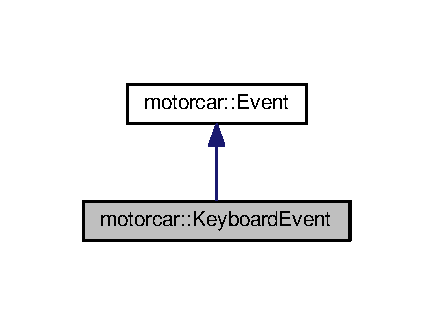
\includegraphics[width=208pt]{classmotorcar_1_1KeyboardEvent__inherit__graph}
\end{center}
\end{figure}


Collaboration diagram for motorcar\-:\-:Keyboard\-Event\-:
\nopagebreak
\begin{figure}[H]
\begin{center}
\leavevmode
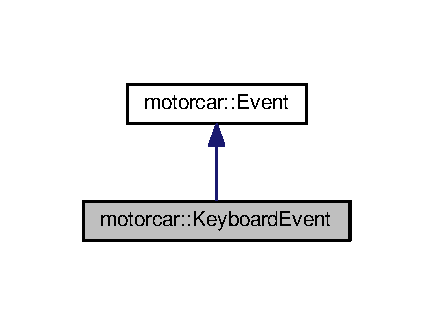
\includegraphics[width=208pt]{classmotorcar_1_1KeyboardEvent__coll__graph}
\end{center}
\end{figure}
\subsection*{Public Types}
\begin{DoxyCompactItemize}
\item 
enum \hyperlink{classmotorcar_1_1KeyboardEvent_a160494213466e8fd37ad7b84f0246df6}{Event} \{ \hyperlink{classmotorcar_1_1KeyboardEvent_a160494213466e8fd37ad7b84f0246df6a76edf2c02e4795738cfebfa7d46f499c}{K\-E\-Y\-\_\-\-P\-R\-E\-S\-S}, 
\hyperlink{classmotorcar_1_1KeyboardEvent_a160494213466e8fd37ad7b84f0246df6a592f2e816c45ea3722c81bf7e8aab187}{K\-E\-Y\-\_\-\-R\-E\-L\-E\-A\-S\-E}
 \}
\end{DoxyCompactItemize}
\subsection*{Public Member Functions}
\begin{DoxyCompactItemize}
\item 
\hyperlink{classmotorcar_1_1KeyboardEvent_a06138cdfae36aa5cc374f921ff66f868}{Keyboard\-Event} (\hyperlink{classmotorcar_1_1KeyboardEvent_a160494213466e8fd37ad7b84f0246df6}{Keyboard\-Event\-::\-Event} \hyperlink{classmotorcar_1_1KeyboardEvent_afcaf3f2e053934ccea4b1b44869e8e16}{event}, uint32\-\_\-t \hyperlink{classmotorcar_1_1KeyboardEvent_a1bb9217c0f442aef7f1aa2461e9e6cf4}{key\-Code}, \hyperlink{classmotorcar_1_1Seat}{Seat} $\ast$\hyperlink{classmotorcar_1_1Event_a7426828c8402193cac63a7b3fda5a17e}{seat})
\item 
\hyperlink{classmotorcar_1_1Event_af4f5d9ed7dc2d8a2324fa5b0d32c29b0}{Event\-Type} \hyperlink{classmotorcar_1_1KeyboardEvent_abb35a59eab2d715433ef46868a69df68}{type} () const override
\item 
\hyperlink{classmotorcar_1_1KeyboardEvent_a160494213466e8fd37ad7b84f0246df6}{Keyboard\-Event\-::\-Event} \hyperlink{classmotorcar_1_1KeyboardEvent_afcaf3f2e053934ccea4b1b44869e8e16}{event} () const 
\item 
uint32\-\_\-t \hyperlink{classmotorcar_1_1KeyboardEvent_a1bb9217c0f442aef7f1aa2461e9e6cf4}{key\-Code} () const 
\end{DoxyCompactItemize}


\subsection{Member Enumeration Documentation}
\hypertarget{classmotorcar_1_1KeyboardEvent_a160494213466e8fd37ad7b84f0246df6}{\index{motorcar\-::\-Keyboard\-Event@{motorcar\-::\-Keyboard\-Event}!Event@{Event}}
\index{Event@{Event}!motorcar::KeyboardEvent@{motorcar\-::\-Keyboard\-Event}}
\subsubsection[{Event}]{\setlength{\rightskip}{0pt plus 5cm}enum {\bf motorcar\-::\-Keyboard\-Event\-::\-Event}}}\label{classmotorcar_1_1KeyboardEvent_a160494213466e8fd37ad7b84f0246df6}
\begin{Desc}
\item[Enumerator]\par
\begin{description}
\index{K\-E\-Y\-\_\-\-P\-R\-E\-S\-S@{K\-E\-Y\-\_\-\-P\-R\-E\-S\-S}!motorcar\-::\-Keyboard\-Event@{motorcar\-::\-Keyboard\-Event}}\index{motorcar\-::\-Keyboard\-Event@{motorcar\-::\-Keyboard\-Event}!K\-E\-Y\-\_\-\-P\-R\-E\-S\-S@{K\-E\-Y\-\_\-\-P\-R\-E\-S\-S}}\item[{\em 
\hypertarget{classmotorcar_1_1KeyboardEvent_a160494213466e8fd37ad7b84f0246df6a76edf2c02e4795738cfebfa7d46f499c}{K\-E\-Y\-\_\-\-P\-R\-E\-S\-S}\label{classmotorcar_1_1KeyboardEvent_a160494213466e8fd37ad7b84f0246df6a76edf2c02e4795738cfebfa7d46f499c}
}]\index{K\-E\-Y\-\_\-\-R\-E\-L\-E\-A\-S\-E@{K\-E\-Y\-\_\-\-R\-E\-L\-E\-A\-S\-E}!motorcar\-::\-Keyboard\-Event@{motorcar\-::\-Keyboard\-Event}}\index{motorcar\-::\-Keyboard\-Event@{motorcar\-::\-Keyboard\-Event}!K\-E\-Y\-\_\-\-R\-E\-L\-E\-A\-S\-E@{K\-E\-Y\-\_\-\-R\-E\-L\-E\-A\-S\-E}}\item[{\em 
\hypertarget{classmotorcar_1_1KeyboardEvent_a160494213466e8fd37ad7b84f0246df6a592f2e816c45ea3722c81bf7e8aab187}{K\-E\-Y\-\_\-\-R\-E\-L\-E\-A\-S\-E}\label{classmotorcar_1_1KeyboardEvent_a160494213466e8fd37ad7b84f0246df6a592f2e816c45ea3722c81bf7e8aab187}
}]\end{description}
\end{Desc}


\subsection{Constructor \& Destructor Documentation}
\hypertarget{classmotorcar_1_1KeyboardEvent_a06138cdfae36aa5cc374f921ff66f868}{\index{motorcar\-::\-Keyboard\-Event@{motorcar\-::\-Keyboard\-Event}!Keyboard\-Event@{Keyboard\-Event}}
\index{Keyboard\-Event@{Keyboard\-Event}!motorcar::KeyboardEvent@{motorcar\-::\-Keyboard\-Event}}
\subsubsection[{Keyboard\-Event}]{\setlength{\rightskip}{0pt plus 5cm}Keyboard\-Event\-::\-Keyboard\-Event (
\begin{DoxyParamCaption}
\item[{{\bf Keyboard\-Event\-::\-Event}}]{event, }
\item[{uint32\-\_\-t}]{key\-Code, }
\item[{{\bf Seat} $\ast$}]{seat}
\end{DoxyParamCaption}
)}}\label{classmotorcar_1_1KeyboardEvent_a06138cdfae36aa5cc374f921ff66f868}


\subsection{Member Function Documentation}
\hypertarget{classmotorcar_1_1KeyboardEvent_afcaf3f2e053934ccea4b1b44869e8e16}{\index{motorcar\-::\-Keyboard\-Event@{motorcar\-::\-Keyboard\-Event}!event@{event}}
\index{event@{event}!motorcar::KeyboardEvent@{motorcar\-::\-Keyboard\-Event}}
\subsubsection[{event}]{\setlength{\rightskip}{0pt plus 5cm}{\bf Keyboard\-Event\-::\-Event} Keyboard\-Event\-::event (
\begin{DoxyParamCaption}
{}
\end{DoxyParamCaption}
) const}}\label{classmotorcar_1_1KeyboardEvent_afcaf3f2e053934ccea4b1b44869e8e16}
\hypertarget{classmotorcar_1_1KeyboardEvent_a1bb9217c0f442aef7f1aa2461e9e6cf4}{\index{motorcar\-::\-Keyboard\-Event@{motorcar\-::\-Keyboard\-Event}!key\-Code@{key\-Code}}
\index{key\-Code@{key\-Code}!motorcar::KeyboardEvent@{motorcar\-::\-Keyboard\-Event}}
\subsubsection[{key\-Code}]{\setlength{\rightskip}{0pt plus 5cm}uint32\-\_\-t Keyboard\-Event\-::key\-Code (
\begin{DoxyParamCaption}
{}
\end{DoxyParamCaption}
) const}}\label{classmotorcar_1_1KeyboardEvent_a1bb9217c0f442aef7f1aa2461e9e6cf4}
\hypertarget{classmotorcar_1_1KeyboardEvent_abb35a59eab2d715433ef46868a69df68}{\index{motorcar\-::\-Keyboard\-Event@{motorcar\-::\-Keyboard\-Event}!type@{type}}
\index{type@{type}!motorcar::KeyboardEvent@{motorcar\-::\-Keyboard\-Event}}
\subsubsection[{type}]{\setlength{\rightskip}{0pt plus 5cm}{\bf Event\-::\-Event\-Type} Keyboard\-Event\-::type (
\begin{DoxyParamCaption}
{}
\end{DoxyParamCaption}
) const\hspace{0.3cm}{\ttfamily [override]}, {\ttfamily [virtual]}}}\label{classmotorcar_1_1KeyboardEvent_abb35a59eab2d715433ef46868a69df68}


Implements \hyperlink{classmotorcar_1_1Event_a195195c53c024bc76aa0e550ffe438a6}{motorcar\-::\-Event}.



The documentation for this class was generated from the following files\-:\begin{DoxyCompactItemize}
\item 
/home/dave/thesis/motorcar/src/compositor/events/\hyperlink{keyboardevent_8h}{keyboardevent.\-h}\item 
/home/dave/thesis/motorcar/src/compositor/events/\hyperlink{keyboardevent_8cpp}{keyboardevent.\-cpp}\end{DoxyCompactItemize}

\hypertarget{structmotorcar__shell__interface}{\section{motorcar\-\_\-shell\-\_\-interface Struct Reference}
\label{structmotorcar__shell__interface}\index{motorcar\-\_\-shell\-\_\-interface@{motorcar\-\_\-shell\-\_\-interface}}
}


{\ttfamily \#include $<$motorcar-\/server-\/protocol.\-h$>$}

\subsection*{Public Attributes}
\begin{DoxyCompactItemize}
\item 
void($\ast$ \hyperlink{structmotorcar__shell__interface_af2f516fa4585245d6b7db1fbec34419e}{get\-\_\-motorcar\-\_\-surface} )(struct wl\-\_\-client $\ast$client, struct wl\-\_\-resource $\ast$resource, uint32\-\_\-t id, struct wl\-\_\-resource $\ast$\hyperlink{simple-egl_8cpp_a0720952aa1caded45b5bcdce589663a9}{surface}, uint32\-\_\-t clipping\-\_\-mode, uint32\-\_\-t enable\-\_\-depth\-\_\-compositing)
\end{DoxyCompactItemize}


\subsection{Detailed Description}
motorcar\-\_\-shell -\/ a 3\-D compositor shell \-: create a motorcar surface from a surface

An interface to allow a copositor to composite 3\-D data from multiple clients in a manner that makes it appear to be in the same 3\-D space. Combined with embedding tradtional wayland surfaces on quads in the same space it provides the framework needed to achieve a seamless mixture of 2\-D and 3\-D user interfaces while still giving clients full flexibility in how their content is drawn to 2\-D

It allows clients to associate a motorcar\-\_\-surface with a basic surface, which both tells the compositor to perform 3\-D compositing on the client surface, and also provides a mechanism for the compositor to give the client the information it needs to draw its content to 2\-D correctly. 

\subsection{Member Data Documentation}
\hypertarget{structmotorcar__shell__interface_af2f516fa4585245d6b7db1fbec34419e}{\index{motorcar\-\_\-shell\-\_\-interface@{motorcar\-\_\-shell\-\_\-interface}!get\-\_\-motorcar\-\_\-surface@{get\-\_\-motorcar\-\_\-surface}}
\index{get\-\_\-motorcar\-\_\-surface@{get\-\_\-motorcar\-\_\-surface}!motorcar_shell_interface@{motorcar\-\_\-shell\-\_\-interface}}
\subsubsection[{get\-\_\-motorcar\-\_\-surface}]{\setlength{\rightskip}{0pt plus 5cm}void($\ast$ motorcar\-\_\-shell\-\_\-interface\-::get\-\_\-motorcar\-\_\-surface)(struct wl\-\_\-client $\ast$client, struct wl\-\_\-resource $\ast$resource, uint32\-\_\-t id, struct wl\-\_\-resource $\ast${\bf surface}, uint32\-\_\-t clipping\-\_\-mode, uint32\-\_\-t enable\-\_\-depth\-\_\-compositing)}}\label{structmotorcar__shell__interface_af2f516fa4585245d6b7db1fbec34419e}
get\-\_\-motorcar\-\_\-surface -\/ create a motorcar surface from a surface \-: the id of the new motorcar surface to be created \-: the wl\-\_\-surface which the motorcar\-\_\-surface is to be associated with \-: the clipping mode to be used by the compositor for this surface \-: boolean value indicating whether to use depth buffer compositing on this surface

Create a motorcar surface for an existing surface.

Only one motorcar surface can be associated with a given surface. 

The documentation for this struct was generated from the following file\-:\begin{DoxyCompactItemize}
\item 
/home/dave/thesis/motorcar/src/protocol/\hyperlink{motorcar-server-protocol_8h}{motorcar-\/server-\/protocol.\-h}\end{DoxyCompactItemize}

\hypertarget{structmotorcar__six__dof__pointer__interface}{\section{motorcar\-\_\-six\-\_\-dof\-\_\-pointer\-\_\-interface Struct Reference}
\label{structmotorcar__six__dof__pointer__interface}\index{motorcar\-\_\-six\-\_\-dof\-\_\-pointer\-\_\-interface@{motorcar\-\_\-six\-\_\-dof\-\_\-pointer\-\_\-interface}}
}


{\ttfamily \#include $<$motorcar-\/server-\/protocol.\-h$>$}

\subsection*{Public Attributes}
\begin{DoxyCompactItemize}
\item 
void($\ast$ \hyperlink{structmotorcar__six__dof__pointer__interface_af0a50e3dcf962950e332433fc3242d83}{release} )(struct wl\-\_\-client $\ast$client, struct wl\-\_\-resource $\ast$resource)
\end{DoxyCompactItemize}


\subsection{Detailed Description}
motorcar\-\_\-six\-\_\-dof\-\_\-pointer -\/ six degree of freedom pointer input device \-: release the six\-\_\-dof pointer object

This interface represents a six degree of freedom pointing device which behaves much like a traditional pointing device except that rather then event being associated with a 2\-D position they are associated with a 3\-D position and orientation, represented as a 3-\/vector position and column major 3x3 rotation matrix as packed 32 bit float arrays (all values in meters). Most of the events are the same as the traditional wayaland pointer events other than this.

The motorcar\-\_\-six\-\_\-dof\-\_\-pointer interface generates motion, enter and leave events for the surfaces that the six\-\_\-dof pointer is located over, and button and axis events for button presses, button releases and scrolling. 

\subsection{Member Data Documentation}
\hypertarget{structmotorcar__six__dof__pointer__interface_af0a50e3dcf962950e332433fc3242d83}{\index{motorcar\-\_\-six\-\_\-dof\-\_\-pointer\-\_\-interface@{motorcar\-\_\-six\-\_\-dof\-\_\-pointer\-\_\-interface}!release@{release}}
\index{release@{release}!motorcar_six_dof_pointer_interface@{motorcar\-\_\-six\-\_\-dof\-\_\-pointer\-\_\-interface}}
\subsubsection[{release}]{\setlength{\rightskip}{0pt plus 5cm}void($\ast$ motorcar\-\_\-six\-\_\-dof\-\_\-pointer\-\_\-interface\-::release)(struct wl\-\_\-client $\ast$client, struct wl\-\_\-resource $\ast$resource)}}\label{structmotorcar__six__dof__pointer__interface_af0a50e3dcf962950e332433fc3242d83}
release -\/ release the six\-\_\-dof pointer object 

The documentation for this struct was generated from the following file\-:\begin{DoxyCompactItemize}
\item 
/home/dave/thesis/motorcar/src/protocol/\hyperlink{motorcar-server-protocol_8h}{motorcar-\/server-\/protocol.\-h}\end{DoxyCompactItemize}

\hypertarget{structmotorcar__six__dof__pointer__listener}{\section{motorcar\-\_\-six\-\_\-dof\-\_\-pointer\-\_\-listener Struct Reference}
\label{structmotorcar__six__dof__pointer__listener}\index{motorcar\-\_\-six\-\_\-dof\-\_\-pointer\-\_\-listener@{motorcar\-\_\-six\-\_\-dof\-\_\-pointer\-\_\-listener}}
}


{\ttfamily \#include $<$motorcar-\/client-\/protocol.\-h$>$}

\subsection*{Public Attributes}
\begin{DoxyCompactItemize}
\item 
void($\ast$ \hyperlink{structmotorcar__six__dof__pointer__listener_a60aa469977dee03cfe23738b53628c0a}{enter} )(void $\ast$data, struct motorcar\-\_\-six\-\_\-dof\-\_\-pointer $\ast$motorcar\-\_\-six\-\_\-dof\-\_\-pointer, uint32\-\_\-t serial, struct motorcar\-\_\-surface $\ast$\hyperlink{simple-egl_8cpp_a0720952aa1caded45b5bcdce589663a9}{surface}, struct wl\-\_\-array $\ast$position, struct wl\-\_\-array $\ast$orientation)
\item 
void($\ast$ \hyperlink{structmotorcar__six__dof__pointer__listener_ac00b36c868704689626997fd27b407b9}{leave} )(void $\ast$data, struct motorcar\-\_\-six\-\_\-dof\-\_\-pointer $\ast$motorcar\-\_\-six\-\_\-dof\-\_\-pointer, uint32\-\_\-t serial, struct motorcar\-\_\-surface $\ast$\hyperlink{simple-egl_8cpp_a0720952aa1caded45b5bcdce589663a9}{surface})
\item 
void($\ast$ \hyperlink{structmotorcar__six__dof__pointer__listener_ae2701450acd4d0c55f5b0ffa54fad191}{motion} )(void $\ast$data, struct motorcar\-\_\-six\-\_\-dof\-\_\-pointer $\ast$motorcar\-\_\-six\-\_\-dof\-\_\-pointer, uint32\-\_\-t time, struct wl\-\_\-array $\ast$position, struct wl\-\_\-array $\ast$orientation)
\item 
void($\ast$ \hyperlink{structmotorcar__six__dof__pointer__listener_a768d27906b6a34cbe6069bf830f3efdd}{button} )(void $\ast$data, struct motorcar\-\_\-six\-\_\-dof\-\_\-pointer $\ast$motorcar\-\_\-six\-\_\-dof\-\_\-pointer, uint32\-\_\-t serial, uint32\-\_\-t time, uint32\-\_\-t button, uint32\-\_\-t state)
\end{DoxyCompactItemize}


\subsection{Detailed Description}
motorcar\-\_\-six\-\_\-dof\-\_\-pointer -\/ six degree of freedom pointer input device \-: enter event \-: leave event \-: six\-\_\-dof pointer motion event \-: pointer button event

This interface represents a six degree of freedom pointing device which behaves much like a traditional pointing device except that rather then event being associated with a 2\-D position they are associated with a 3\-D position and orientation, represented as a 3-\/vector position and column major 3x3 rotation matrix as packed 32 bit float arrays (all values in meters). Most of the events are the same as the traditional wayaland pointer events other than this.

The motorcar\-\_\-six\-\_\-dof\-\_\-pointer interface generates motion, enter and leave events for the surfaces that the six\-\_\-dof pointer is located over, and button and axis events for button presses, button releases and scrolling. 

\subsection{Member Data Documentation}
\hypertarget{structmotorcar__six__dof__pointer__listener_a768d27906b6a34cbe6069bf830f3efdd}{\index{motorcar\-\_\-six\-\_\-dof\-\_\-pointer\-\_\-listener@{motorcar\-\_\-six\-\_\-dof\-\_\-pointer\-\_\-listener}!button@{button}}
\index{button@{button}!motorcar_six_dof_pointer_listener@{motorcar\-\_\-six\-\_\-dof\-\_\-pointer\-\_\-listener}}
\subsubsection[{button}]{\setlength{\rightskip}{0pt plus 5cm}void($\ast$ motorcar\-\_\-six\-\_\-dof\-\_\-pointer\-\_\-listener\-::button)(void $\ast$data, struct motorcar\-\_\-six\-\_\-dof\-\_\-pointer $\ast$motorcar\-\_\-six\-\_\-dof\-\_\-pointer, uint32\-\_\-t serial, uint32\-\_\-t time, uint32\-\_\-t button, uint32\-\_\-t state)}}\label{structmotorcar__six__dof__pointer__listener_a768d27906b6a34cbe6069bf830f3efdd}
button -\/ pointer button event \-: (none) \-: timestamp with millisecond granularity \-: (none) \-: (none)

Mouse button click and release notifications.

The location of the click is given by the last motion or enter event. The time argument is a timestamp with millisecond granularity, with an undefined base. \hypertarget{structmotorcar__six__dof__pointer__listener_a60aa469977dee03cfe23738b53628c0a}{\index{motorcar\-\_\-six\-\_\-dof\-\_\-pointer\-\_\-listener@{motorcar\-\_\-six\-\_\-dof\-\_\-pointer\-\_\-listener}!enter@{enter}}
\index{enter@{enter}!motorcar_six_dof_pointer_listener@{motorcar\-\_\-six\-\_\-dof\-\_\-pointer\-\_\-listener}}
\subsubsection[{enter}]{\setlength{\rightskip}{0pt plus 5cm}void($\ast$ motorcar\-\_\-six\-\_\-dof\-\_\-pointer\-\_\-listener\-::enter)(void $\ast$data, struct motorcar\-\_\-six\-\_\-dof\-\_\-pointer $\ast$motorcar\-\_\-six\-\_\-dof\-\_\-pointer, uint32\-\_\-t serial, struct motorcar\-\_\-surface $\ast${\bf surface}, struct wl\-\_\-array $\ast$position, struct wl\-\_\-array $\ast$orientation)}}\label{structmotorcar__six__dof__pointer__listener_a60aa469977dee03cfe23738b53628c0a}
enter -\/ enter event \-: (none) \-: (none) \-: position of pointing device in meters at the time of this event, represented as a packed array of three 32 bit floats \-: orientation of the pointing device in meters at the time of this event, represented as a packed column major 3x3 rotation matrix of 32 bit floats

Notification that this seat's six\-\_\-dof pointer is focused on a certain surface. \hypertarget{structmotorcar__six__dof__pointer__listener_ac00b36c868704689626997fd27b407b9}{\index{motorcar\-\_\-six\-\_\-dof\-\_\-pointer\-\_\-listener@{motorcar\-\_\-six\-\_\-dof\-\_\-pointer\-\_\-listener}!leave@{leave}}
\index{leave@{leave}!motorcar_six_dof_pointer_listener@{motorcar\-\_\-six\-\_\-dof\-\_\-pointer\-\_\-listener}}
\subsubsection[{leave}]{\setlength{\rightskip}{0pt plus 5cm}void($\ast$ motorcar\-\_\-six\-\_\-dof\-\_\-pointer\-\_\-listener\-::leave)(void $\ast$data, struct motorcar\-\_\-six\-\_\-dof\-\_\-pointer $\ast$motorcar\-\_\-six\-\_\-dof\-\_\-pointer, uint32\-\_\-t serial, struct motorcar\-\_\-surface $\ast${\bf surface})}}\label{structmotorcar__six__dof__pointer__listener_ac00b36c868704689626997fd27b407b9}
leave -\/ leave event \-: (none) \-: (none)

Notification that this seat's six\-\_\-dof pointer is no longer focused on a certain surface.

The leave notification is sent before the enter notification for the new focus. \hypertarget{structmotorcar__six__dof__pointer__listener_ae2701450acd4d0c55f5b0ffa54fad191}{\index{motorcar\-\_\-six\-\_\-dof\-\_\-pointer\-\_\-listener@{motorcar\-\_\-six\-\_\-dof\-\_\-pointer\-\_\-listener}!motion@{motion}}
\index{motion@{motion}!motorcar_six_dof_pointer_listener@{motorcar\-\_\-six\-\_\-dof\-\_\-pointer\-\_\-listener}}
\subsubsection[{motion}]{\setlength{\rightskip}{0pt plus 5cm}void($\ast$ motorcar\-\_\-six\-\_\-dof\-\_\-pointer\-\_\-listener\-::motion)(void $\ast$data, struct motorcar\-\_\-six\-\_\-dof\-\_\-pointer $\ast$motorcar\-\_\-six\-\_\-dof\-\_\-pointer, uint32\-\_\-t time, struct wl\-\_\-array $\ast$position, struct wl\-\_\-array $\ast$orientation)}}\label{structmotorcar__six__dof__pointer__listener_ae2701450acd4d0c55f5b0ffa54fad191}
motion -\/ six\-\_\-dof pointer motion event \-: timestamp with millisecond granularity \-: position of pointing device in meters at the time of this event, represented as a packed array of three 32 bit floats \-: orientation of the pointing device in meters at the time of this event, represented as a packed column major 3x3 rotation matrix of 32 bit floats

Notification of six\-\_\-dof pointer location change. The arguments are the postion and orientation of the six\-\_\-dof pointer device 

The documentation for this struct was generated from the following file\-:\begin{DoxyCompactItemize}
\item 
/home/dave/thesis/motorcar/src/protocol/\hyperlink{motorcar-client-protocol_8h}{motorcar-\/client-\/protocol.\-h}\end{DoxyCompactItemize}

\hypertarget{structmotorcar__surface__interface}{\section{motorcar\-\_\-surface\-\_\-interface Struct Reference}
\label{structmotorcar__surface__interface}\index{motorcar\-\_\-surface\-\_\-interface@{motorcar\-\_\-surface\-\_\-interface}}
}


{\ttfamily \#include $<$motorcar-\/server-\/protocol.\-h$>$}

\subsection*{Public Attributes}
\begin{DoxyCompactItemize}
\item 
void($\ast$ \hyperlink{structmotorcar__surface__interface_a0fc3dd0d7064b7885b62cd7733d212b3}{set\-\_\-size\-\_\-3d} )(struct wl\-\_\-client $\ast$client, struct wl\-\_\-resource $\ast$resource, struct wl\-\_\-array $\ast$dimensions)
\end{DoxyCompactItemize}


\subsection{Detailed Description}
motorcar\-\_\-surface -\/ a 3\-D, view dependent, depth composited meta-\/data surface \-: requests that the client resize the 3\-D window to the given scale

An interface that may be implemented by a wl\-\_\-surface, for implementations that provide motorcar style depth composited 3\-D surfaces

A motorcar\-\_\-surface can be created from an exisitng surface, and provides the client with the information needed to draw its content in a way that can be depth composited by a motorcar compliant compositor.

A motorcar surface is handled in the compositor as a 3\-D analog of a traditional window. Rather than the window being a 2 dimensional region of a 2 dimensional interface space, the window represents a 3 dimensional region of a 3 dimensional interface space, essentially a 3\-D box in which the client can draw 3\-D geometry

The 3\-D window has its own 3\-D space whose origin is at the center of the window. The window's position refers to the location of this origin in the world space, and its rotation is around this point. The window also has a 3\-D size, which is defined in its local space. Each component of the size indicates one dimension of the window bounds, so the window extends for one half this distance on each side of the origin in its local space. 

\subsection{Member Data Documentation}
\hypertarget{structmotorcar__surface__interface_a0fc3dd0d7064b7885b62cd7733d212b3}{\index{motorcar\-\_\-surface\-\_\-interface@{motorcar\-\_\-surface\-\_\-interface}!set\-\_\-size\-\_\-3d@{set\-\_\-size\-\_\-3d}}
\index{set\-\_\-size\-\_\-3d@{set\-\_\-size\-\_\-3d}!motorcar_surface_interface@{motorcar\-\_\-surface\-\_\-interface}}
\subsubsection[{set\-\_\-size\-\_\-3d}]{\setlength{\rightskip}{0pt plus 5cm}void($\ast$ motorcar\-\_\-surface\-\_\-interface\-::set\-\_\-size\-\_\-3d)(struct wl\-\_\-client $\ast$client, struct wl\-\_\-resource $\ast$resource, struct wl\-\_\-array $\ast$dimensions)}}\label{structmotorcar__surface__interface_a0fc3dd0d7064b7885b62cd7733d212b3}
set\-\_\-size\-\_\-3d -\/ requests that the client resize the 3\-D window to the given scale \-: the new size vector

Sets the new size of the 3\-D window. If this size is larger than the size most recently requested by the compositor the compositor is free to clip the window to a new size, provided that it immediatly requests the client resize to those dimensions.

The size is represented here as a vector of three 32-\/bit floats, representing the size of the 3\-D window along each of the cardinal axes in the window's local space. 

The documentation for this struct was generated from the following file\-:\begin{DoxyCompactItemize}
\item 
/home/dave/thesis/motorcar/src/protocol/\hyperlink{motorcar-server-protocol_8h}{motorcar-\/server-\/protocol.\-h}\end{DoxyCompactItemize}

\hypertarget{structmotorcar__surface__listener}{\section{motorcar\-\_\-surface\-\_\-listener Struct Reference}
\label{structmotorcar__surface__listener}\index{motorcar\-\_\-surface\-\_\-listener@{motorcar\-\_\-surface\-\_\-listener}}
}


{\ttfamily \#include $<$motorcar-\/client-\/protocol.\-h$>$}

\subsection*{Public Attributes}
\begin{DoxyCompactItemize}
\item 
void($\ast$ \hyperlink{structmotorcar__surface__listener_af82c86b66c3207618e167315173d757c}{transform\-\_\-matrix} )(void $\ast$data, struct motorcar\-\_\-surface $\ast$motorcar\-\_\-surface, struct wl\-\_\-array $\ast$transform)
\item 
void($\ast$ \hyperlink{structmotorcar__surface__listener_aaf93856b0517537beddea51838634496}{request\-\_\-size\-\_\-3d} )(void $\ast$data, struct motorcar\-\_\-surface $\ast$motorcar\-\_\-surface, struct wl\-\_\-array $\ast$dimensions)
\end{DoxyCompactItemize}


\subsection{Detailed Description}
motorcar\-\_\-surface -\/ a 3\-D, view dependent, depth composited meta-\/data surface \-: sets the tranformation of the 3\-D window \-: requests that the client resize the 3\-D window to the given scale

An interface that may be implemented by a wl\-\_\-surface, for implementations that provide motorcar style depth composited 3\-D surfaces

A motorcar\-\_\-surface can be created from an exisitng surface, and provides the client with the information needed to draw its content in a way that can be depth composited by a motorcar compliant compositor.

A motorcar surface is handled in the compositor as a 3\-D analog of a traditional window. Rather than the window being a 2 dimensional region of a 2 dimensional interface space, the window represents a 3 dimensional region of a 3 dimensional interface space, essentially a 3\-D box in which the client can draw 3\-D geometry

The 3\-D window has its own 3\-D space whose origin is at the center of the window. The window's position refers to the location of this origin in the world space, and its rotation is around this point. The window also has a 3\-D size, which is defined in its local space. Each component of the size indicates one dimension of the window bounds, so the window extends for one half this distance on each side of the origin in its local space. 

\subsection{Member Data Documentation}
\hypertarget{structmotorcar__surface__listener_aaf93856b0517537beddea51838634496}{\index{motorcar\-\_\-surface\-\_\-listener@{motorcar\-\_\-surface\-\_\-listener}!request\-\_\-size\-\_\-3d@{request\-\_\-size\-\_\-3d}}
\index{request\-\_\-size\-\_\-3d@{request\-\_\-size\-\_\-3d}!motorcar_surface_listener@{motorcar\-\_\-surface\-\_\-listener}}
\subsubsection[{request\-\_\-size\-\_\-3d}]{\setlength{\rightskip}{0pt plus 5cm}void($\ast$ motorcar\-\_\-surface\-\_\-listener\-::request\-\_\-size\-\_\-3d)(void $\ast$data, struct motorcar\-\_\-surface $\ast$motorcar\-\_\-surface, struct wl\-\_\-array $\ast$dimensions)}}\label{structmotorcar__surface__listener_aaf93856b0517537beddea51838634496}
request\-\_\-size\-\_\-3d -\/ requests that the client resize the 3\-D window to the given scale \-: the requested size vector

Allows the compositor to request the window take a new size. Much like the traditional 2\-D size mechanisms, the compositor cannot set this explicitly, rather, it can only request that the client take a certain dimension, and the client then chooses any size which fits completely within the requested size and sends a resize event back to the compositor.

The size is represented here as a vector of three 32-\/bit floats, representing the size of the 3\-D window along each of the cardinal axes in the window's local space. \hypertarget{structmotorcar__surface__listener_af82c86b66c3207618e167315173d757c}{\index{motorcar\-\_\-surface\-\_\-listener@{motorcar\-\_\-surface\-\_\-listener}!transform\-\_\-matrix@{transform\-\_\-matrix}}
\index{transform\-\_\-matrix@{transform\-\_\-matrix}!motorcar_surface_listener@{motorcar\-\_\-surface\-\_\-listener}}
\subsubsection[{transform\-\_\-matrix}]{\setlength{\rightskip}{0pt plus 5cm}void($\ast$ motorcar\-\_\-surface\-\_\-listener\-::transform\-\_\-matrix)(void $\ast$data, struct motorcar\-\_\-surface $\ast$motorcar\-\_\-surface, struct wl\-\_\-array $\ast$transform)}}\label{structmotorcar__surface__listener_af82c86b66c3207618e167315173d757c}
transform\-\_\-matrix -\/ sets the tranformation of the 3\-D window \-: the new transform matrix

This event is sent to indicate a change in the transform of the client's 3\-D window

This matrix can be though of as the model matrix for the client's 3\-D window, which brings vectors from the window local space into world space.

It is represented here as a column-\/major 4x4 matrix of 32 bit floats, with all values are specified in meters. 

The documentation for this struct was generated from the following file\-:\begin{DoxyCompactItemize}
\item 
/home/dave/thesis/motorcar/src/protocol/\hyperlink{motorcar-client-protocol_8h}{motorcar-\/client-\/protocol.\-h}\end{DoxyCompactItemize}

\hypertarget{structmotorcar__viewpoint__listener}{\section{motorcar\-\_\-viewpoint\-\_\-listener Struct Reference}
\label{structmotorcar__viewpoint__listener}\index{motorcar\-\_\-viewpoint\-\_\-listener@{motorcar\-\_\-viewpoint\-\_\-listener}}
}


{\ttfamily \#include $<$motorcar-\/client-\/protocol.\-h$>$}

\subsection*{Public Attributes}
\begin{DoxyCompactItemize}
\item 
void($\ast$ \hyperlink{structmotorcar__viewpoint__listener_a62bcafc2fde2470d81ea8bce70855af5}{view\-\_\-matrix} )(void $\ast$data, struct motorcar\-\_\-viewpoint $\ast$motorcar\-\_\-viewpoint, struct wl\-\_\-array $\ast$view)
\item 
void($\ast$ \hyperlink{structmotorcar__viewpoint__listener_ac3811e768cf181e5c3c4377fd11816d8}{projection\-\_\-matrix} )(void $\ast$data, struct motorcar\-\_\-viewpoint $\ast$motorcar\-\_\-viewpoint, struct wl\-\_\-array $\ast$projection)
\item 
void($\ast$ \hyperlink{structmotorcar__viewpoint__listener_a0b3a306b14550df2000169a8984d925f}{view\-\_\-port} )(void $\ast$data, struct motorcar\-\_\-viewpoint $\ast$motorcar\-\_\-viewpoint, int32\-\_\-t color\-\_\-x, int32\-\_\-t color\-\_\-y, uint32\-\_\-t color\-\_\-width, uint32\-\_\-t color\-\_\-height, int32\-\_\-t depth\-\_\-x, int32\-\_\-t depth\-\_\-y, uint32\-\_\-t depth\-\_\-width, uint32\-\_\-t depth\-\_\-height)
\end{DoxyCompactItemize}


\subsection{Detailed Description}
motorcar\-\_\-viewpoint -\/ represents a single viewpoint in the compositor, essentially a view and projection matrix \-: sets the view matrix of this viewpoint for the next frame \-: change the projection matrix of this viewpoint \-: sets the view ports of this viewpoint to be used when rendering into motorcar surface buffers

This interface represents a viewpoint (essentially a virtual camera) in the compositor's 3\-D compositing space, and the events it contains are designed to keep the compositor and client viewpoints synced so that the viewpoints in the client and compositor space stay consistent; 

\subsection{Member Data Documentation}
\hypertarget{structmotorcar__viewpoint__listener_ac3811e768cf181e5c3c4377fd11816d8}{\index{motorcar\-\_\-viewpoint\-\_\-listener@{motorcar\-\_\-viewpoint\-\_\-listener}!projection\-\_\-matrix@{projection\-\_\-matrix}}
\index{projection\-\_\-matrix@{projection\-\_\-matrix}!motorcar_viewpoint_listener@{motorcar\-\_\-viewpoint\-\_\-listener}}
\subsubsection[{projection\-\_\-matrix}]{\setlength{\rightskip}{0pt plus 5cm}void($\ast$ motorcar\-\_\-viewpoint\-\_\-listener\-::projection\-\_\-matrix)(void $\ast$data, struct motorcar\-\_\-viewpoint $\ast$motorcar\-\_\-viewpoint, struct wl\-\_\-array $\ast$projection)}}\label{structmotorcar__viewpoint__listener_ac3811e768cf181e5c3c4377fd11816d8}
projection\-\_\-matrix -\/ change the projection matrix of this viewpoint \-: the new projection matrix for this viewpoint

This event is sent immediately after the viewpoint global is bound by the client, and is only resent if the projection matrix for this viewpoint changes in the compoisitor (which would be unusual but is certainly possible)

This matrix is in the form of the projection matrices used by Open\-G\-L, which (with the help of a homogeneous divide done in hardware) brings vectors from view space into uniform device coordinate space in which vertices are projected from 3\-D to 2\-D.

It is represented here as a column-\/major 4x4 matrix of 32 bit floats, with all values are specified in meters. \hypertarget{structmotorcar__viewpoint__listener_a62bcafc2fde2470d81ea8bce70855af5}{\index{motorcar\-\_\-viewpoint\-\_\-listener@{motorcar\-\_\-viewpoint\-\_\-listener}!view\-\_\-matrix@{view\-\_\-matrix}}
\index{view\-\_\-matrix@{view\-\_\-matrix}!motorcar_viewpoint_listener@{motorcar\-\_\-viewpoint\-\_\-listener}}
\subsubsection[{view\-\_\-matrix}]{\setlength{\rightskip}{0pt plus 5cm}void($\ast$ motorcar\-\_\-viewpoint\-\_\-listener\-::view\-\_\-matrix)(void $\ast$data, struct motorcar\-\_\-viewpoint $\ast$motorcar\-\_\-viewpoint, struct wl\-\_\-array $\ast$view)}}\label{structmotorcar__viewpoint__listener_a62bcafc2fde2470d81ea8bce70855af5}
view\-\_\-matrix -\/ sets the view matrix of this viewpoint for the next frame \-: the view matrix for this frame

This event is sent (ideally) at the beginning of each frame to give the client the view matrix it needs to draw its content to 2\-D in the same manner as the compositor.

This matrix is the view matrix, which brings vectors from world space into view (or camera) space, which is the inverse of the camera transform. \hypertarget{structmotorcar__viewpoint__listener_a0b3a306b14550df2000169a8984d925f}{\index{motorcar\-\_\-viewpoint\-\_\-listener@{motorcar\-\_\-viewpoint\-\_\-listener}!view\-\_\-port@{view\-\_\-port}}
\index{view\-\_\-port@{view\-\_\-port}!motorcar_viewpoint_listener@{motorcar\-\_\-viewpoint\-\_\-listener}}
\subsubsection[{view\-\_\-port}]{\setlength{\rightskip}{0pt plus 5cm}void($\ast$ motorcar\-\_\-viewpoint\-\_\-listener\-::view\-\_\-port)(void $\ast$data, struct motorcar\-\_\-viewpoint $\ast$motorcar\-\_\-viewpoint, int32\-\_\-t color\-\_\-x, int32\-\_\-t color\-\_\-y, uint32\-\_\-t color\-\_\-width, uint32\-\_\-t color\-\_\-height, int32\-\_\-t depth\-\_\-x, int32\-\_\-t depth\-\_\-y, uint32\-\_\-t depth\-\_\-width, uint32\-\_\-t depth\-\_\-height)}}\label{structmotorcar__viewpoint__listener_a0b3a306b14550df2000169a8984d925f}
view\-\_\-port -\/ sets the view ports of this viewpoint to be used when rendering into motorcar surface buffers \-: x position of the color viewport, in pixels \-: y position of the color viewport, in pixels \-: width of the color viewport, in pixels \-: height of the color viewport, in pixels \-: x position of the depth viewport, in pixels \-: y position of the depth viewport, in pixels \-: width of the depth viewport, in pixels \-: height of the depth viewport, in pixels

This event tells the client where in its surface buffer it needs to draw the output associated with this viewpoint, which allows the compositor to extract the correct output for each viewpoint. Like the projection matrix, this event is sent immediately after the client binds this viewpoint global and is only sent again if the viewport changes on the compositor side.

Viewport consists of a position and a size in surface local coordinates. Each viewpoint has two viewports associated with it, one to hold the color buffer from the client, and one to hold the depth buffer contents (which is encoded in the color buffer since E\-G\-L does not support a color mode that includes depth). If an E\-G\-L extension was written which creates a format that includes the depth buffer, then the depth viewport could hypothetically be ignored when that extension was present. 

The documentation for this struct was generated from the following file\-:\begin{DoxyCompactItemize}
\item 
/media/dave/e89b5eb4-\/4b10-\/4edf-\/8ad5-\/0d046a46b978/dave/thesis/qtwayland-\/motorcar-\/compositor/motorcar/clients/simple-\/egl/\hyperlink{clients_2simple-egl_2motorcar-client-protocol_8h}{motorcar-\/client-\/protocol.\-h}\end{DoxyCompactItemize}

\hypertarget{classmotorcar_1_1MotorcarSurfaceNode}{\section{motorcar\-:\-:Motorcar\-Surface\-Node Class Reference}
\label{classmotorcar_1_1MotorcarSurfaceNode}\index{motorcar\-::\-Motorcar\-Surface\-Node@{motorcar\-::\-Motorcar\-Surface\-Node}}
}


{\ttfamily \#include $<$motorcarsurfacenode.\-h$>$}



Inheritance diagram for motorcar\-:\-:Motorcar\-Surface\-Node\-:
\nopagebreak
\begin{figure}[H]
\begin{center}
\leavevmode
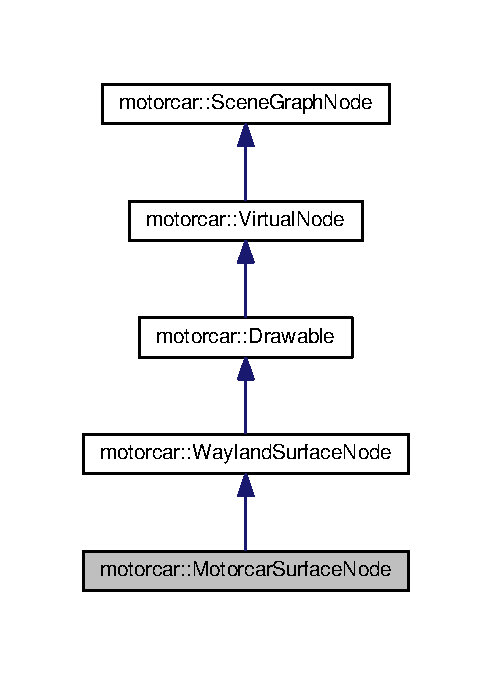
\includegraphics[width=236pt]{classmotorcar_1_1MotorcarSurfaceNode__inherit__graph}
\end{center}
\end{figure}


Collaboration diagram for motorcar\-:\-:Motorcar\-Surface\-Node\-:
\nopagebreak
\begin{figure}[H]
\begin{center}
\leavevmode
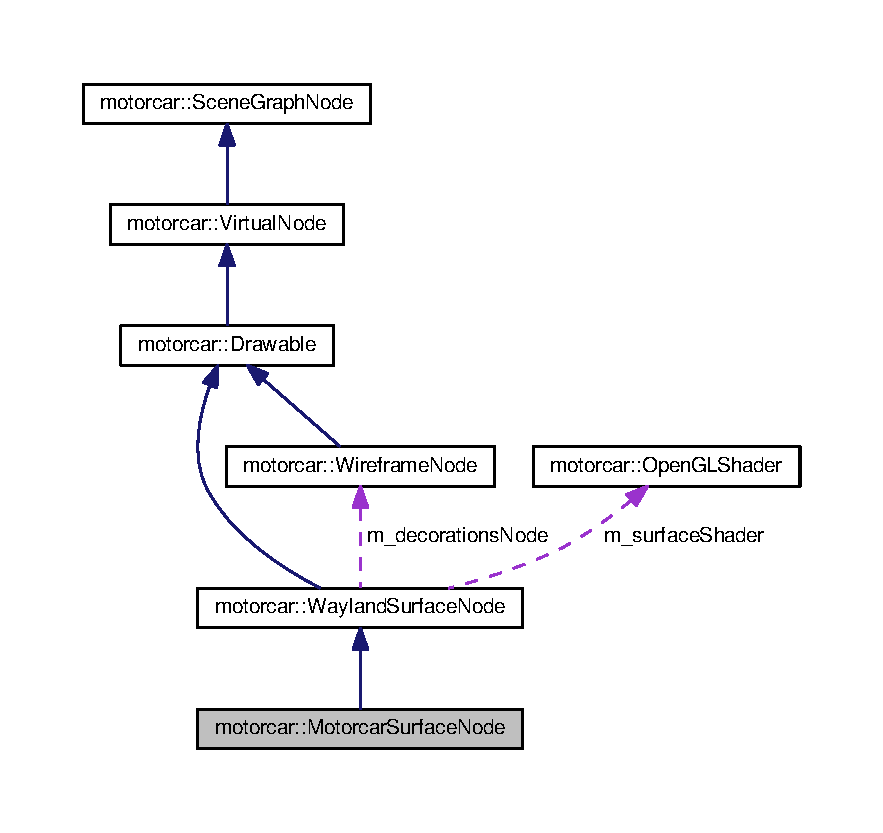
\includegraphics[width=350pt]{classmotorcar_1_1MotorcarSurfaceNode__coll__graph}
\end{center}
\end{figure}
\subsection*{Public Member Functions}
\begin{DoxyCompactItemize}
\item 
\hyperlink{classmotorcar_1_1MotorcarSurfaceNode_aab75702ea552e4d9df6edece3dcd5328}{Motorcar\-Surface\-Node} (\hyperlink{classmotorcar_1_1WaylandSurface}{Wayland\-Surface} $\ast$\hyperlink{simple-egl_8cpp_a0720952aa1caded45b5bcdce589663a9}{surface}, \hyperlink{classmotorcar_1_1SceneGraphNode}{Scene\-Graph\-Node} $\ast$parent, const glm\-::mat4 \&\hyperlink{classmotorcar_1_1SceneGraphNode_ad96e79fdd739ac8223a3128003be391a}{transform}=glm\-::mat4(1), glm\-::vec3 \hyperlink{classmotorcar_1_1MotorcarSurfaceNode_a83b83213c56f85783a948e28fb5b11b0}{dimensions}=glm\-::vec3(1))
\item 
virtual void \hyperlink{classmotorcar_1_1MotorcarSurfaceNode_afe8227366d3644d09d13c905ff2d86a8}{draw} (\hyperlink{classmotorcar_1_1Scene}{Scene} $\ast$\hyperlink{classmotorcar_1_1SceneGraphNode_aa14e637ed4ae98f77e28941a4b5cfdd8}{scene}, \hyperlink{classmotorcar_1_1Display}{Display} $\ast$\hyperlink{structdisplay}{display}) override
\begin{DoxyCompactList}\small\item\em extracts the depth and color information from the client surface, clips them against the surface boundaries, and composites with the scene \end{DoxyCompactList}\item 
virtual void \hyperlink{classmotorcar_1_1MotorcarSurfaceNode_ab0c7df201ceb2d73c1077daf90574016}{compute\-Surface\-Transform} (float ppcm) override
\begin{DoxyCompactList}\small\item\em computes surface transform \end{DoxyCompactList}\item 
void \hyperlink{classmotorcar_1_1MotorcarSurfaceNode_a21eac7e80d2855fcb822541abc7f1965}{handle\-World\-Transform\-Change} (\hyperlink{classmotorcar_1_1Scene}{Scene} $\ast$\hyperlink{classmotorcar_1_1SceneGraphNode_aa14e637ed4ae98f77e28941a4b5cfdd8}{scene}) override
\begin{DoxyCompactList}\small\item\em react to changes in the node's worldtransform \end{DoxyCompactList}\item 
glm\-::vec3 \hyperlink{classmotorcar_1_1MotorcarSurfaceNode_a83b83213c56f85783a948e28fb5b11b0}{dimensions} () const 
\item 
void \hyperlink{classmotorcar_1_1MotorcarSurfaceNode_aa58a458e928fb175ebbddc2c4c501a17}{request\-Size3\-D} (const glm\-::vec3 \&\hyperlink{classmotorcar_1_1MotorcarSurfaceNode_a83b83213c56f85783a948e28fb5b11b0}{dimensions})
\item 
wl\-\_\-resource $\ast$ \hyperlink{classmotorcar_1_1MotorcarSurfaceNode_aea6b1f37432c263f4256e87e940018f8}{resource} () const 
\item 
void \hyperlink{classmotorcar_1_1MotorcarSurfaceNode_a9bf1d1d9ce0df9e34b3a9410861a6a96}{configure\-Resource} (struct wl\-\_\-client $\ast$client, uint32\-\_\-t id)
\end{DoxyCompactItemize}
\subsection*{Static Public Member Functions}
\begin{DoxyCompactItemize}
\item 
static void \hyperlink{classmotorcar_1_1MotorcarSurfaceNode_aa3cd0c916984418ef2a093c1bcb5b29a}{handle\-\_\-set\-\_\-size\-\_\-3d} (struct wl\-\_\-client $\ast$client, struct wl\-\_\-resource $\ast$\hyperlink{classmotorcar_1_1MotorcarSurfaceNode_aea6b1f37432c263f4256e87e940018f8}{resource}, struct wl\-\_\-array $\ast$\hyperlink{classmotorcar_1_1MotorcarSurfaceNode_a83b83213c56f85783a948e28fb5b11b0}{dimensions})
\end{DoxyCompactItemize}
\subsection*{Additional Inherited Members}


\subsection{Constructor \& Destructor Documentation}
\hypertarget{classmotorcar_1_1MotorcarSurfaceNode_aab75702ea552e4d9df6edece3dcd5328}{\index{motorcar\-::\-Motorcar\-Surface\-Node@{motorcar\-::\-Motorcar\-Surface\-Node}!Motorcar\-Surface\-Node@{Motorcar\-Surface\-Node}}
\index{Motorcar\-Surface\-Node@{Motorcar\-Surface\-Node}!motorcar::MotorcarSurfaceNode@{motorcar\-::\-Motorcar\-Surface\-Node}}
\subsubsection[{Motorcar\-Surface\-Node}]{\setlength{\rightskip}{0pt plus 5cm}Motorcar\-Surface\-Node\-::\-Motorcar\-Surface\-Node (
\begin{DoxyParamCaption}
\item[{{\bf Wayland\-Surface} $\ast$}]{surface, }
\item[{{\bf Scene\-Graph\-Node} $\ast$}]{parent, }
\item[{const glm\-::mat4 \&}]{transform = {\ttfamily glm\-:\-:mat4(1)}, }
\item[{glm\-::vec3}]{dimensions = {\ttfamily glm\-:\-:vec3(1)}}
\end{DoxyParamCaption}
)}}\label{classmotorcar_1_1MotorcarSurfaceNode_aab75702ea552e4d9df6edece3dcd5328}


\subsection{Member Function Documentation}
\hypertarget{classmotorcar_1_1MotorcarSurfaceNode_ab0c7df201ceb2d73c1077daf90574016}{\index{motorcar\-::\-Motorcar\-Surface\-Node@{motorcar\-::\-Motorcar\-Surface\-Node}!compute\-Surface\-Transform@{compute\-Surface\-Transform}}
\index{compute\-Surface\-Transform@{compute\-Surface\-Transform}!motorcar::MotorcarSurfaceNode@{motorcar\-::\-Motorcar\-Surface\-Node}}
\subsubsection[{compute\-Surface\-Transform}]{\setlength{\rightskip}{0pt plus 5cm}void Motorcar\-Surface\-Node\-::compute\-Surface\-Transform (
\begin{DoxyParamCaption}
\item[{float}]{ppcm}
\end{DoxyParamCaption}
)\hspace{0.3cm}{\ttfamily [override]}, {\ttfamily [virtual]}}}\label{classmotorcar_1_1MotorcarSurfaceNode_ab0c7df201ceb2d73c1077daf90574016}


computes surface transform 



Reimplemented from \hyperlink{classmotorcar_1_1WaylandSurfaceNode_a0dfac06ca2855e41613b6e663c76c97e}{motorcar\-::\-Wayland\-Surface\-Node}.

\hypertarget{classmotorcar_1_1MotorcarSurfaceNode_a9bf1d1d9ce0df9e34b3a9410861a6a96}{\index{motorcar\-::\-Motorcar\-Surface\-Node@{motorcar\-::\-Motorcar\-Surface\-Node}!configure\-Resource@{configure\-Resource}}
\index{configure\-Resource@{configure\-Resource}!motorcar::MotorcarSurfaceNode@{motorcar\-::\-Motorcar\-Surface\-Node}}
\subsubsection[{configure\-Resource}]{\setlength{\rightskip}{0pt plus 5cm}void Motorcar\-Surface\-Node\-::configure\-Resource (
\begin{DoxyParamCaption}
\item[{struct wl\-\_\-client $\ast$}]{client, }
\item[{uint32\-\_\-t}]{id}
\end{DoxyParamCaption}
)}}\label{classmotorcar_1_1MotorcarSurfaceNode_a9bf1d1d9ce0df9e34b3a9410861a6a96}
\hypertarget{classmotorcar_1_1MotorcarSurfaceNode_a83b83213c56f85783a948e28fb5b11b0}{\index{motorcar\-::\-Motorcar\-Surface\-Node@{motorcar\-::\-Motorcar\-Surface\-Node}!dimensions@{dimensions}}
\index{dimensions@{dimensions}!motorcar::MotorcarSurfaceNode@{motorcar\-::\-Motorcar\-Surface\-Node}}
\subsubsection[{dimensions}]{\setlength{\rightskip}{0pt plus 5cm}glm\-::vec3 Motorcar\-Surface\-Node\-::dimensions (
\begin{DoxyParamCaption}
{}
\end{DoxyParamCaption}
) const}}\label{classmotorcar_1_1MotorcarSurfaceNode_a83b83213c56f85783a948e28fb5b11b0}
\hypertarget{classmotorcar_1_1MotorcarSurfaceNode_afe8227366d3644d09d13c905ff2d86a8}{\index{motorcar\-::\-Motorcar\-Surface\-Node@{motorcar\-::\-Motorcar\-Surface\-Node}!draw@{draw}}
\index{draw@{draw}!motorcar::MotorcarSurfaceNode@{motorcar\-::\-Motorcar\-Surface\-Node}}
\subsubsection[{draw}]{\setlength{\rightskip}{0pt plus 5cm}void Motorcar\-Surface\-Node\-::draw (
\begin{DoxyParamCaption}
\item[{{\bf Scene} $\ast$}]{scene, }
\item[{{\bf Display} $\ast$}]{display}
\end{DoxyParamCaption}
)\hspace{0.3cm}{\ttfamily [override]}, {\ttfamily [virtual]}}}\label{classmotorcar_1_1MotorcarSurfaceNode_afe8227366d3644d09d13c905ff2d86a8}


extracts the depth and color information from the client surface, clips them against the surface boundaries, and composites with the scene 



Reimplemented from \hyperlink{classmotorcar_1_1WaylandSurfaceNode_a1afe3178777574dd1b3c66d7d19d871b}{motorcar\-::\-Wayland\-Surface\-Node}.

\hypertarget{classmotorcar_1_1MotorcarSurfaceNode_aa3cd0c916984418ef2a093c1bcb5b29a}{\index{motorcar\-::\-Motorcar\-Surface\-Node@{motorcar\-::\-Motorcar\-Surface\-Node}!handle\-\_\-set\-\_\-size\-\_\-3d@{handle\-\_\-set\-\_\-size\-\_\-3d}}
\index{handle\-\_\-set\-\_\-size\-\_\-3d@{handle\-\_\-set\-\_\-size\-\_\-3d}!motorcar::MotorcarSurfaceNode@{motorcar\-::\-Motorcar\-Surface\-Node}}
\subsubsection[{handle\-\_\-set\-\_\-size\-\_\-3d}]{\setlength{\rightskip}{0pt plus 5cm}void Motorcar\-Surface\-Node\-::handle\-\_\-set\-\_\-size\-\_\-3d (
\begin{DoxyParamCaption}
\item[{struct wl\-\_\-client $\ast$}]{client, }
\item[{struct wl\-\_\-resource $\ast$}]{resource, }
\item[{struct wl\-\_\-array $\ast$}]{dimensions}
\end{DoxyParamCaption}
)\hspace{0.3cm}{\ttfamily [static]}}}\label{classmotorcar_1_1MotorcarSurfaceNode_aa3cd0c916984418ef2a093c1bcb5b29a}
\hypertarget{classmotorcar_1_1MotorcarSurfaceNode_a21eac7e80d2855fcb822541abc7f1965}{\index{motorcar\-::\-Motorcar\-Surface\-Node@{motorcar\-::\-Motorcar\-Surface\-Node}!handle\-World\-Transform\-Change@{handle\-World\-Transform\-Change}}
\index{handle\-World\-Transform\-Change@{handle\-World\-Transform\-Change}!motorcar::MotorcarSurfaceNode@{motorcar\-::\-Motorcar\-Surface\-Node}}
\subsubsection[{handle\-World\-Transform\-Change}]{\setlength{\rightskip}{0pt plus 5cm}void Motorcar\-Surface\-Node\-::handle\-World\-Transform\-Change (
\begin{DoxyParamCaption}
\item[{{\bf Scene} $\ast$}]{scene}
\end{DoxyParamCaption}
)\hspace{0.3cm}{\ttfamily [override]}, {\ttfamily [virtual]}}}\label{classmotorcar_1_1MotorcarSurfaceNode_a21eac7e80d2855fcb822541abc7f1965}


react to changes in the node's worldtransform 



Reimplemented from \hyperlink{classmotorcar_1_1SceneGraphNode_ad81e5f74bf448c2be1dc9f536d6d98b6}{motorcar\-::\-Scene\-Graph\-Node}.

\hypertarget{classmotorcar_1_1MotorcarSurfaceNode_aa58a458e928fb175ebbddc2c4c501a17}{\index{motorcar\-::\-Motorcar\-Surface\-Node@{motorcar\-::\-Motorcar\-Surface\-Node}!request\-Size3\-D@{request\-Size3\-D}}
\index{request\-Size3\-D@{request\-Size3\-D}!motorcar::MotorcarSurfaceNode@{motorcar\-::\-Motorcar\-Surface\-Node}}
\subsubsection[{request\-Size3\-D}]{\setlength{\rightskip}{0pt plus 5cm}void Motorcar\-Surface\-Node\-::request\-Size3\-D (
\begin{DoxyParamCaption}
\item[{const glm\-::vec3 \&}]{dimensions}
\end{DoxyParamCaption}
)}}\label{classmotorcar_1_1MotorcarSurfaceNode_aa58a458e928fb175ebbddc2c4c501a17}
\hypertarget{classmotorcar_1_1MotorcarSurfaceNode_aea6b1f37432c263f4256e87e940018f8}{\index{motorcar\-::\-Motorcar\-Surface\-Node@{motorcar\-::\-Motorcar\-Surface\-Node}!resource@{resource}}
\index{resource@{resource}!motorcar::MotorcarSurfaceNode@{motorcar\-::\-Motorcar\-Surface\-Node}}
\subsubsection[{resource}]{\setlength{\rightskip}{0pt plus 5cm}wl\-\_\-resource $\ast$ Motorcar\-Surface\-Node\-::resource (
\begin{DoxyParamCaption}
{}
\end{DoxyParamCaption}
) const}}\label{classmotorcar_1_1MotorcarSurfaceNode_aea6b1f37432c263f4256e87e940018f8}


The documentation for this class was generated from the following files\-:\begin{DoxyCompactItemize}
\item 
/home/dave/thesis/motorcar/src/compositor/scenegraph/output/wayland/\hyperlink{motorcarsurfacenode_8h}{motorcarsurfacenode.\-h}\item 
/home/dave/thesis/motorcar/src/compositor/scenegraph/output/wayland/\hyperlink{motorcarsurfacenode_8cpp}{motorcarsurfacenode.\-cpp}\end{DoxyCompactItemize}

\hypertarget{structmotorsurface__listener}{\section{motorsurface\-\_\-listener Struct Reference}
\label{structmotorsurface__listener}\index{motorsurface\-\_\-listener@{motorsurface\-\_\-listener}}
}
\subsection*{Public Attributes}
\begin{DoxyCompactItemize}
\item 
\hyperlink{structmotorsurface__listener_a4d4b3119171f1602c0882696545a8921}{motorcar\-\_\-surface\-\_\-handle\-\_\-transform\-\_\-matrix}
\end{DoxyCompactItemize}


\subsection{Member Data Documentation}
\hypertarget{structmotorsurface__listener_a4d4b3119171f1602c0882696545a8921}{\index{motorsurface\-\_\-listener@{motorsurface\-\_\-listener}!motorcar\-\_\-surface\-\_\-handle\-\_\-transform\-\_\-matrix@{motorcar\-\_\-surface\-\_\-handle\-\_\-transform\-\_\-matrix}}
\index{motorcar\-\_\-surface\-\_\-handle\-\_\-transform\-\_\-matrix@{motorcar\-\_\-surface\-\_\-handle\-\_\-transform\-\_\-matrix}!motorsurface_listener@{motorsurface\-\_\-listener}}
\subsubsection[{motorcar\-\_\-surface\-\_\-handle\-\_\-transform\-\_\-matrix}]{\setlength{\rightskip}{0pt plus 5cm}motorsurface\-\_\-listener\-::motorcar\-\_\-surface\-\_\-handle\-\_\-transform\-\_\-matrix}}\label{structmotorsurface__listener_a4d4b3119171f1602c0882696545a8921}


The documentation for this struct was generated from the following file\-:\begin{DoxyCompactItemize}
\item 
/home/dave/thesis/motorcar/src/examples/clients/simple-\/egl/\hyperlink{simple-egl_8cpp}{simple-\/egl.\-cpp}\end{DoxyCompactItemize}

\hypertarget{classmotorcar_1_1MouseEvent}{\section{motorcar\-:\-:Mouse\-Event Class Reference}
\label{classmotorcar_1_1MouseEvent}\index{motorcar\-::\-Mouse\-Event@{motorcar\-::\-Mouse\-Event}}
}


{\ttfamily \#include $<$mouseevent.\-h$>$}



Inheritance diagram for motorcar\-:\-:Mouse\-Event\-:
\nopagebreak
\begin{figure}[H]
\begin{center}
\leavevmode
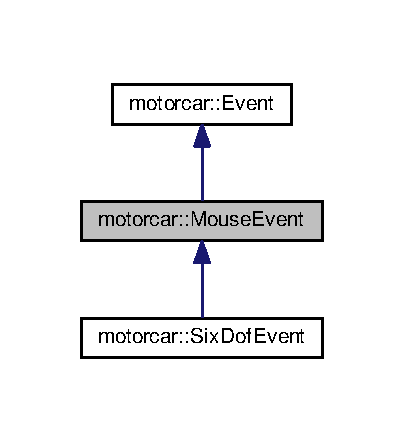
\includegraphics[width=194pt]{classmotorcar_1_1MouseEvent__inherit__graph}
\end{center}
\end{figure}


Collaboration diagram for motorcar\-:\-:Mouse\-Event\-:
\nopagebreak
\begin{figure}[H]
\begin{center}
\leavevmode
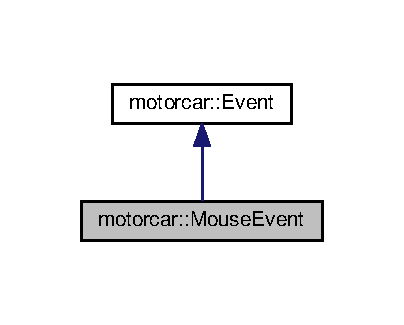
\includegraphics[width=194pt]{classmotorcar_1_1MouseEvent__coll__graph}
\end{center}
\end{figure}
\subsection*{Public Types}
\begin{DoxyCompactItemize}
\item 
enum \hyperlink{classmotorcar_1_1MouseEvent_a2d063fb053a90c196b58c1dec4d989aa}{Event} \{ \\*
\hyperlink{classmotorcar_1_1MouseEvent_a2d063fb053a90c196b58c1dec4d989aaa566f527f2ad7bd86d18ae6fc33cd0d15}{B\-U\-T\-T\-O\-N\-\_\-\-P\-R\-E\-S\-S}, 
\hyperlink{classmotorcar_1_1MouseEvent_a2d063fb053a90c196b58c1dec4d989aaab71770cff8c9b00629bf59ec4fa806c4}{B\-U\-T\-T\-O\-N\-\_\-\-R\-E\-L\-E\-A\-S\-E}, 
\hyperlink{classmotorcar_1_1MouseEvent_a2d063fb053a90c196b58c1dec4d989aaa679f8c98a12aeb73e9e3891cf48a964a}{M\-O\-V\-E}, 
\hyperlink{classmotorcar_1_1MouseEvent_a2d063fb053a90c196b58c1dec4d989aaa5c13df864239249ca5c25fc29db3243e}{E\-N\-T\-E\-R}, 
\\*
\hyperlink{classmotorcar_1_1MouseEvent_a2d063fb053a90c196b58c1dec4d989aaa87474f39e7a1771a9068ca5498e8399e}{L\-E\-A\-V\-E}
 \}
\item 
enum \hyperlink{classmotorcar_1_1MouseEvent_aeb5515c2434123ce2f897f8fc89effae}{Button} \{ \hyperlink{classmotorcar_1_1MouseEvent_aeb5515c2434123ce2f897f8fc89effaead2303cd4e996a291b8a55dff0d44130c}{L\-E\-F\-T}, 
\hyperlink{classmotorcar_1_1MouseEvent_aeb5515c2434123ce2f897f8fc89effaea9988f559d0b0dc2ecd80f7325a7091e2}{R\-I\-G\-H\-T}, 
\hyperlink{classmotorcar_1_1MouseEvent_aeb5515c2434123ce2f897f8fc89effaea7e41ded0faa1ee5f90c5df6adc9d76c3}{M\-I\-D\-D\-L\-E}, 
\hyperlink{classmotorcar_1_1MouseEvent_aeb5515c2434123ce2f897f8fc89effaea18194aa8373867605b8527cbb1d268a8}{N\-O\-N\-E}
 \}
\end{DoxyCompactItemize}
\subsection*{Public Member Functions}
\begin{DoxyCompactItemize}
\item 
\hyperlink{classmotorcar_1_1MouseEvent_ac29d5c7d5c7e4176828f2b671458c25b}{Mouse\-Event} (\hyperlink{classmotorcar_1_1MouseEvent_a2d063fb053a90c196b58c1dec4d989aa}{Mouse\-Event\-::\-Event} \hyperlink{classmotorcar_1_1MouseEvent_a52d0060d0793eab0ca6aad7f69d78fda}{event}, \hyperlink{classmotorcar_1_1MouseEvent_aeb5515c2434123ce2f897f8fc89effae}{Mouse\-Event\-::\-Button} \hyperlink{classmotorcar_1_1MouseEvent_a6682d4092f940335170806435e3bb6fe}{button}, glm\-::vec2 local\-Postion, \hyperlink{classmotorcar_1_1Seat}{Seat} $\ast$\hyperlink{classmotorcar_1_1Event_a7426828c8402193cac63a7b3fda5a17e}{seat})
\item 
\hyperlink{classmotorcar_1_1Event_af4f5d9ed7dc2d8a2324fa5b0d32c29b0}{Event\-Type} \hyperlink{classmotorcar_1_1MouseEvent_afb419c29a7d2fa6dd429eeb3ac0699c5}{type} () const override
\item 
\hyperlink{classmotorcar_1_1MouseEvent_a2d063fb053a90c196b58c1dec4d989aa}{Mouse\-Event\-::\-Event} \hyperlink{classmotorcar_1_1MouseEvent_a52d0060d0793eab0ca6aad7f69d78fda}{event} () const 
\item 
\hyperlink{classmotorcar_1_1MouseEvent_aeb5515c2434123ce2f897f8fc89effae}{Mouse\-Event\-::\-Button} \hyperlink{classmotorcar_1_1MouseEvent_a6682d4092f940335170806435e3bb6fe}{button} () const 
\item 
glm\-::vec2 \hyperlink{classmotorcar_1_1MouseEvent_aaadbd8608dd2e0ed6d3836f0947f2141}{local\-Position} () const 
\end{DoxyCompactItemize}


\subsection{Member Enumeration Documentation}
\hypertarget{classmotorcar_1_1MouseEvent_aeb5515c2434123ce2f897f8fc89effae}{\index{motorcar\-::\-Mouse\-Event@{motorcar\-::\-Mouse\-Event}!Button@{Button}}
\index{Button@{Button}!motorcar::MouseEvent@{motorcar\-::\-Mouse\-Event}}
\subsubsection[{Button}]{\setlength{\rightskip}{0pt plus 5cm}enum {\bf motorcar\-::\-Mouse\-Event\-::\-Button}}}\label{classmotorcar_1_1MouseEvent_aeb5515c2434123ce2f897f8fc89effae}
\begin{Desc}
\item[Enumerator]\par
\begin{description}
\index{L\-E\-F\-T@{L\-E\-F\-T}!motorcar\-::\-Mouse\-Event@{motorcar\-::\-Mouse\-Event}}\index{motorcar\-::\-Mouse\-Event@{motorcar\-::\-Mouse\-Event}!L\-E\-F\-T@{L\-E\-F\-T}}\item[{\em 
\hypertarget{classmotorcar_1_1MouseEvent_aeb5515c2434123ce2f897f8fc89effaead2303cd4e996a291b8a55dff0d44130c}{L\-E\-F\-T}\label{classmotorcar_1_1MouseEvent_aeb5515c2434123ce2f897f8fc89effaead2303cd4e996a291b8a55dff0d44130c}
}]\index{R\-I\-G\-H\-T@{R\-I\-G\-H\-T}!motorcar\-::\-Mouse\-Event@{motorcar\-::\-Mouse\-Event}}\index{motorcar\-::\-Mouse\-Event@{motorcar\-::\-Mouse\-Event}!R\-I\-G\-H\-T@{R\-I\-G\-H\-T}}\item[{\em 
\hypertarget{classmotorcar_1_1MouseEvent_aeb5515c2434123ce2f897f8fc89effaea9988f559d0b0dc2ecd80f7325a7091e2}{R\-I\-G\-H\-T}\label{classmotorcar_1_1MouseEvent_aeb5515c2434123ce2f897f8fc89effaea9988f559d0b0dc2ecd80f7325a7091e2}
}]\index{M\-I\-D\-D\-L\-E@{M\-I\-D\-D\-L\-E}!motorcar\-::\-Mouse\-Event@{motorcar\-::\-Mouse\-Event}}\index{motorcar\-::\-Mouse\-Event@{motorcar\-::\-Mouse\-Event}!M\-I\-D\-D\-L\-E@{M\-I\-D\-D\-L\-E}}\item[{\em 
\hypertarget{classmotorcar_1_1MouseEvent_aeb5515c2434123ce2f897f8fc89effaea7e41ded0faa1ee5f90c5df6adc9d76c3}{M\-I\-D\-D\-L\-E}\label{classmotorcar_1_1MouseEvent_aeb5515c2434123ce2f897f8fc89effaea7e41ded0faa1ee5f90c5df6adc9d76c3}
}]\index{N\-O\-N\-E@{N\-O\-N\-E}!motorcar\-::\-Mouse\-Event@{motorcar\-::\-Mouse\-Event}}\index{motorcar\-::\-Mouse\-Event@{motorcar\-::\-Mouse\-Event}!N\-O\-N\-E@{N\-O\-N\-E}}\item[{\em 
\hypertarget{classmotorcar_1_1MouseEvent_aeb5515c2434123ce2f897f8fc89effaea18194aa8373867605b8527cbb1d268a8}{N\-O\-N\-E}\label{classmotorcar_1_1MouseEvent_aeb5515c2434123ce2f897f8fc89effaea18194aa8373867605b8527cbb1d268a8}
}]\end{description}
\end{Desc}
\hypertarget{classmotorcar_1_1MouseEvent_a2d063fb053a90c196b58c1dec4d989aa}{\index{motorcar\-::\-Mouse\-Event@{motorcar\-::\-Mouse\-Event}!Event@{Event}}
\index{Event@{Event}!motorcar::MouseEvent@{motorcar\-::\-Mouse\-Event}}
\subsubsection[{Event}]{\setlength{\rightskip}{0pt plus 5cm}enum {\bf motorcar\-::\-Mouse\-Event\-::\-Event}}}\label{classmotorcar_1_1MouseEvent_a2d063fb053a90c196b58c1dec4d989aa}
\begin{Desc}
\item[Enumerator]\par
\begin{description}
\index{B\-U\-T\-T\-O\-N\-\_\-\-P\-R\-E\-S\-S@{B\-U\-T\-T\-O\-N\-\_\-\-P\-R\-E\-S\-S}!motorcar\-::\-Mouse\-Event@{motorcar\-::\-Mouse\-Event}}\index{motorcar\-::\-Mouse\-Event@{motorcar\-::\-Mouse\-Event}!B\-U\-T\-T\-O\-N\-\_\-\-P\-R\-E\-S\-S@{B\-U\-T\-T\-O\-N\-\_\-\-P\-R\-E\-S\-S}}\item[{\em 
\hypertarget{classmotorcar_1_1MouseEvent_a2d063fb053a90c196b58c1dec4d989aaa566f527f2ad7bd86d18ae6fc33cd0d15}{B\-U\-T\-T\-O\-N\-\_\-\-P\-R\-E\-S\-S}\label{classmotorcar_1_1MouseEvent_a2d063fb053a90c196b58c1dec4d989aaa566f527f2ad7bd86d18ae6fc33cd0d15}
}]\index{B\-U\-T\-T\-O\-N\-\_\-\-R\-E\-L\-E\-A\-S\-E@{B\-U\-T\-T\-O\-N\-\_\-\-R\-E\-L\-E\-A\-S\-E}!motorcar\-::\-Mouse\-Event@{motorcar\-::\-Mouse\-Event}}\index{motorcar\-::\-Mouse\-Event@{motorcar\-::\-Mouse\-Event}!B\-U\-T\-T\-O\-N\-\_\-\-R\-E\-L\-E\-A\-S\-E@{B\-U\-T\-T\-O\-N\-\_\-\-R\-E\-L\-E\-A\-S\-E}}\item[{\em 
\hypertarget{classmotorcar_1_1MouseEvent_a2d063fb053a90c196b58c1dec4d989aaab71770cff8c9b00629bf59ec4fa806c4}{B\-U\-T\-T\-O\-N\-\_\-\-R\-E\-L\-E\-A\-S\-E}\label{classmotorcar_1_1MouseEvent_a2d063fb053a90c196b58c1dec4d989aaab71770cff8c9b00629bf59ec4fa806c4}
}]\index{M\-O\-V\-E@{M\-O\-V\-E}!motorcar\-::\-Mouse\-Event@{motorcar\-::\-Mouse\-Event}}\index{motorcar\-::\-Mouse\-Event@{motorcar\-::\-Mouse\-Event}!M\-O\-V\-E@{M\-O\-V\-E}}\item[{\em 
\hypertarget{classmotorcar_1_1MouseEvent_a2d063fb053a90c196b58c1dec4d989aaa679f8c98a12aeb73e9e3891cf48a964a}{M\-O\-V\-E}\label{classmotorcar_1_1MouseEvent_a2d063fb053a90c196b58c1dec4d989aaa679f8c98a12aeb73e9e3891cf48a964a}
}]\index{E\-N\-T\-E\-R@{E\-N\-T\-E\-R}!motorcar\-::\-Mouse\-Event@{motorcar\-::\-Mouse\-Event}}\index{motorcar\-::\-Mouse\-Event@{motorcar\-::\-Mouse\-Event}!E\-N\-T\-E\-R@{E\-N\-T\-E\-R}}\item[{\em 
\hypertarget{classmotorcar_1_1MouseEvent_a2d063fb053a90c196b58c1dec4d989aaa5c13df864239249ca5c25fc29db3243e}{E\-N\-T\-E\-R}\label{classmotorcar_1_1MouseEvent_a2d063fb053a90c196b58c1dec4d989aaa5c13df864239249ca5c25fc29db3243e}
}]\index{L\-E\-A\-V\-E@{L\-E\-A\-V\-E}!motorcar\-::\-Mouse\-Event@{motorcar\-::\-Mouse\-Event}}\index{motorcar\-::\-Mouse\-Event@{motorcar\-::\-Mouse\-Event}!L\-E\-A\-V\-E@{L\-E\-A\-V\-E}}\item[{\em 
\hypertarget{classmotorcar_1_1MouseEvent_a2d063fb053a90c196b58c1dec4d989aaa87474f39e7a1771a9068ca5498e8399e}{L\-E\-A\-V\-E}\label{classmotorcar_1_1MouseEvent_a2d063fb053a90c196b58c1dec4d989aaa87474f39e7a1771a9068ca5498e8399e}
}]\end{description}
\end{Desc}


\subsection{Constructor \& Destructor Documentation}
\hypertarget{classmotorcar_1_1MouseEvent_ac29d5c7d5c7e4176828f2b671458c25b}{\index{motorcar\-::\-Mouse\-Event@{motorcar\-::\-Mouse\-Event}!Mouse\-Event@{Mouse\-Event}}
\index{Mouse\-Event@{Mouse\-Event}!motorcar::MouseEvent@{motorcar\-::\-Mouse\-Event}}
\subsubsection[{Mouse\-Event}]{\setlength{\rightskip}{0pt plus 5cm}Mouse\-Event\-::\-Mouse\-Event (
\begin{DoxyParamCaption}
\item[{{\bf Mouse\-Event\-::\-Event}}]{event, }
\item[{{\bf Mouse\-Event\-::\-Button}}]{button, }
\item[{glm\-::vec2}]{local\-Postion, }
\item[{{\bf Seat} $\ast$}]{seat}
\end{DoxyParamCaption}
)}}\label{classmotorcar_1_1MouseEvent_ac29d5c7d5c7e4176828f2b671458c25b}


\subsection{Member Function Documentation}
\hypertarget{classmotorcar_1_1MouseEvent_a6682d4092f940335170806435e3bb6fe}{\index{motorcar\-::\-Mouse\-Event@{motorcar\-::\-Mouse\-Event}!button@{button}}
\index{button@{button}!motorcar::MouseEvent@{motorcar\-::\-Mouse\-Event}}
\subsubsection[{button}]{\setlength{\rightskip}{0pt plus 5cm}{\bf Mouse\-Event\-::\-Button} Mouse\-Event\-::button (
\begin{DoxyParamCaption}
{}
\end{DoxyParamCaption}
) const}}\label{classmotorcar_1_1MouseEvent_a6682d4092f940335170806435e3bb6fe}
\hypertarget{classmotorcar_1_1MouseEvent_a52d0060d0793eab0ca6aad7f69d78fda}{\index{motorcar\-::\-Mouse\-Event@{motorcar\-::\-Mouse\-Event}!event@{event}}
\index{event@{event}!motorcar::MouseEvent@{motorcar\-::\-Mouse\-Event}}
\subsubsection[{event}]{\setlength{\rightskip}{0pt plus 5cm}{\bf Mouse\-Event\-::\-Event} Mouse\-Event\-::event (
\begin{DoxyParamCaption}
{}
\end{DoxyParamCaption}
) const}}\label{classmotorcar_1_1MouseEvent_a52d0060d0793eab0ca6aad7f69d78fda}
\hypertarget{classmotorcar_1_1MouseEvent_aaadbd8608dd2e0ed6d3836f0947f2141}{\index{motorcar\-::\-Mouse\-Event@{motorcar\-::\-Mouse\-Event}!local\-Position@{local\-Position}}
\index{local\-Position@{local\-Position}!motorcar::MouseEvent@{motorcar\-::\-Mouse\-Event}}
\subsubsection[{local\-Position}]{\setlength{\rightskip}{0pt plus 5cm}glm\-::vec2 Mouse\-Event\-::local\-Position (
\begin{DoxyParamCaption}
{}
\end{DoxyParamCaption}
) const}}\label{classmotorcar_1_1MouseEvent_aaadbd8608dd2e0ed6d3836f0947f2141}
\hypertarget{classmotorcar_1_1MouseEvent_afb419c29a7d2fa6dd429eeb3ac0699c5}{\index{motorcar\-::\-Mouse\-Event@{motorcar\-::\-Mouse\-Event}!type@{type}}
\index{type@{type}!motorcar::MouseEvent@{motorcar\-::\-Mouse\-Event}}
\subsubsection[{type}]{\setlength{\rightskip}{0pt plus 5cm}{\bf Event\-::\-Event\-Type} Mouse\-Event\-::type (
\begin{DoxyParamCaption}
{}
\end{DoxyParamCaption}
) const\hspace{0.3cm}{\ttfamily [override]}, {\ttfamily [virtual]}}}\label{classmotorcar_1_1MouseEvent_afb419c29a7d2fa6dd429eeb3ac0699c5}


Implements \hyperlink{classmotorcar_1_1Event_a195195c53c024bc76aa0e550ffe438a6}{motorcar\-::\-Event}.



The documentation for this class was generated from the following files\-:\begin{DoxyCompactItemize}
\item 
/home/dave/thesis/motorcar/src/compositor/events/\hyperlink{mouseevent_8h}{mouseevent.\-h}\item 
/home/dave/thesis/motorcar/src/compositor/events/\hyperlink{mouseevent_8cpp}{mouseevent.\-cpp}\end{DoxyCompactItemize}

\hypertarget{classmotorcar_1_1OculusHMD}{\section{motorcar\-:\-:Oculus\-H\-M\-D Class Reference}
\label{classmotorcar_1_1OculusHMD}\index{motorcar\-::\-Oculus\-H\-M\-D@{motorcar\-::\-Oculus\-H\-M\-D}}
}


{\ttfamily \#include $<$oculushmd.\-h$>$}



Inheritance diagram for motorcar\-:\-:Oculus\-H\-M\-D\-:
\nopagebreak
\begin{figure}[H]
\begin{center}
\leavevmode
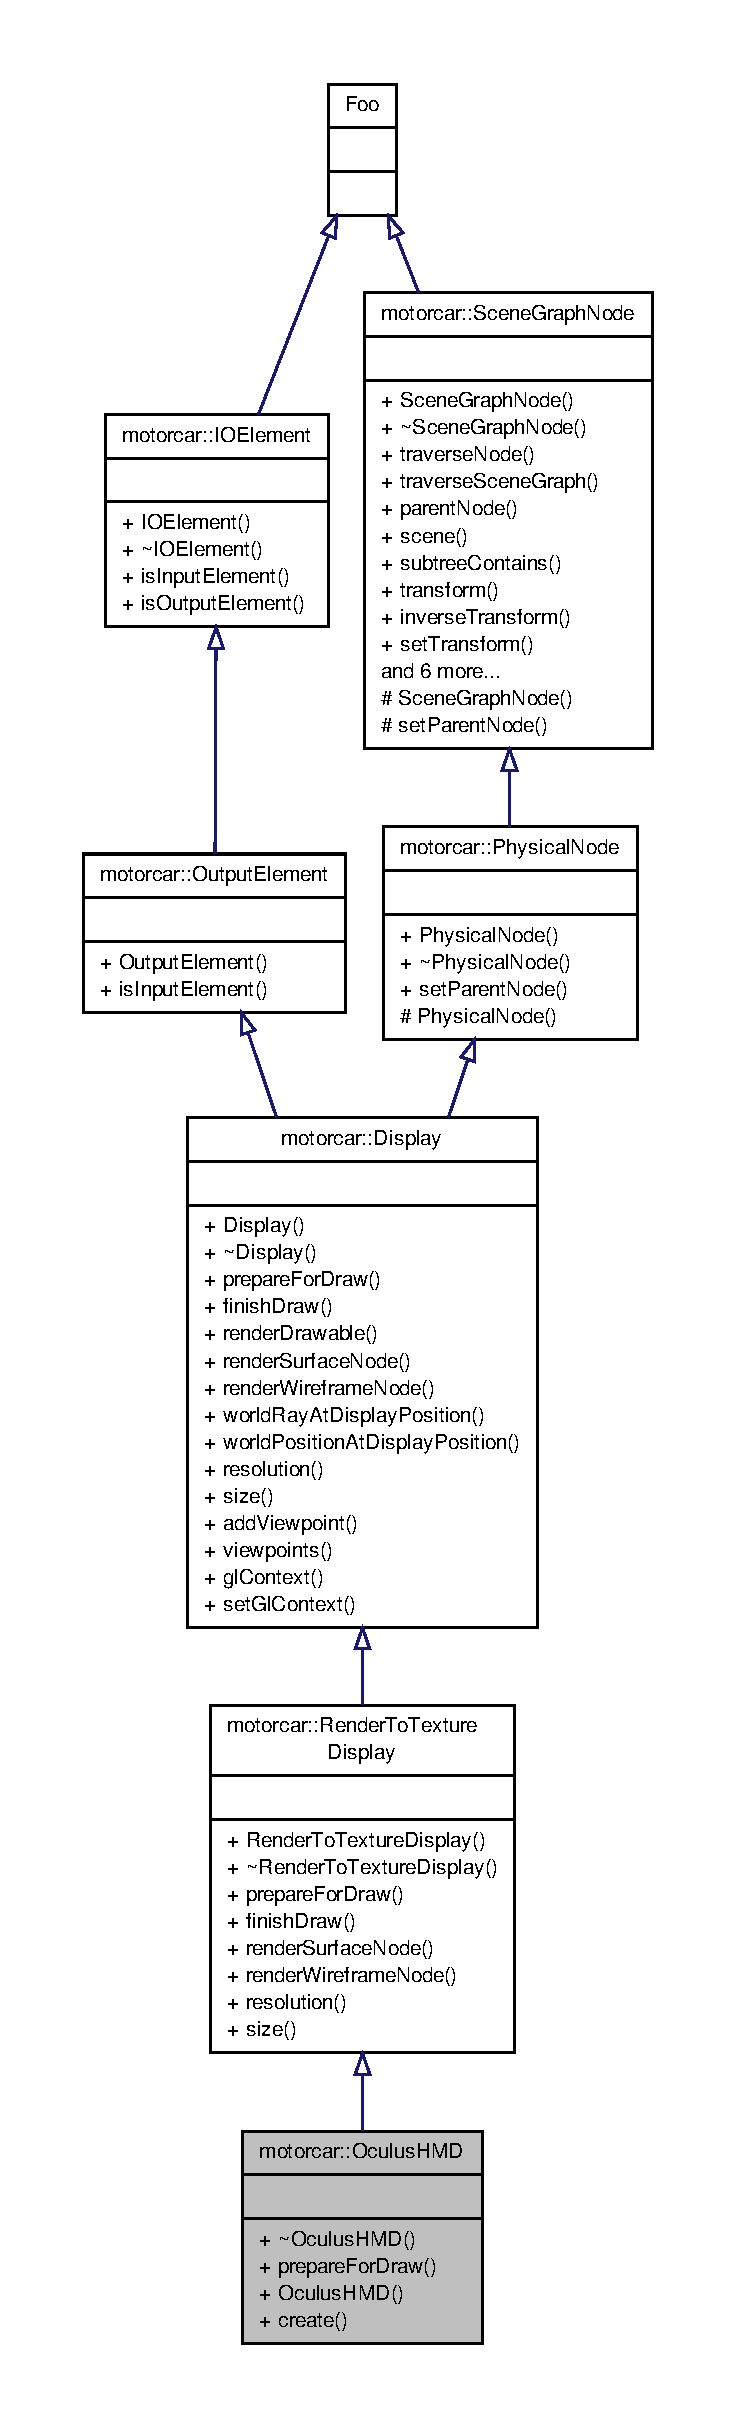
\includegraphics[width=332pt]{classmotorcar_1_1OculusHMD__inherit__graph}
\end{center}
\end{figure}


Collaboration diagram for motorcar\-:\-:Oculus\-H\-M\-D\-:
\nopagebreak
\begin{figure}[H]
\begin{center}
\leavevmode
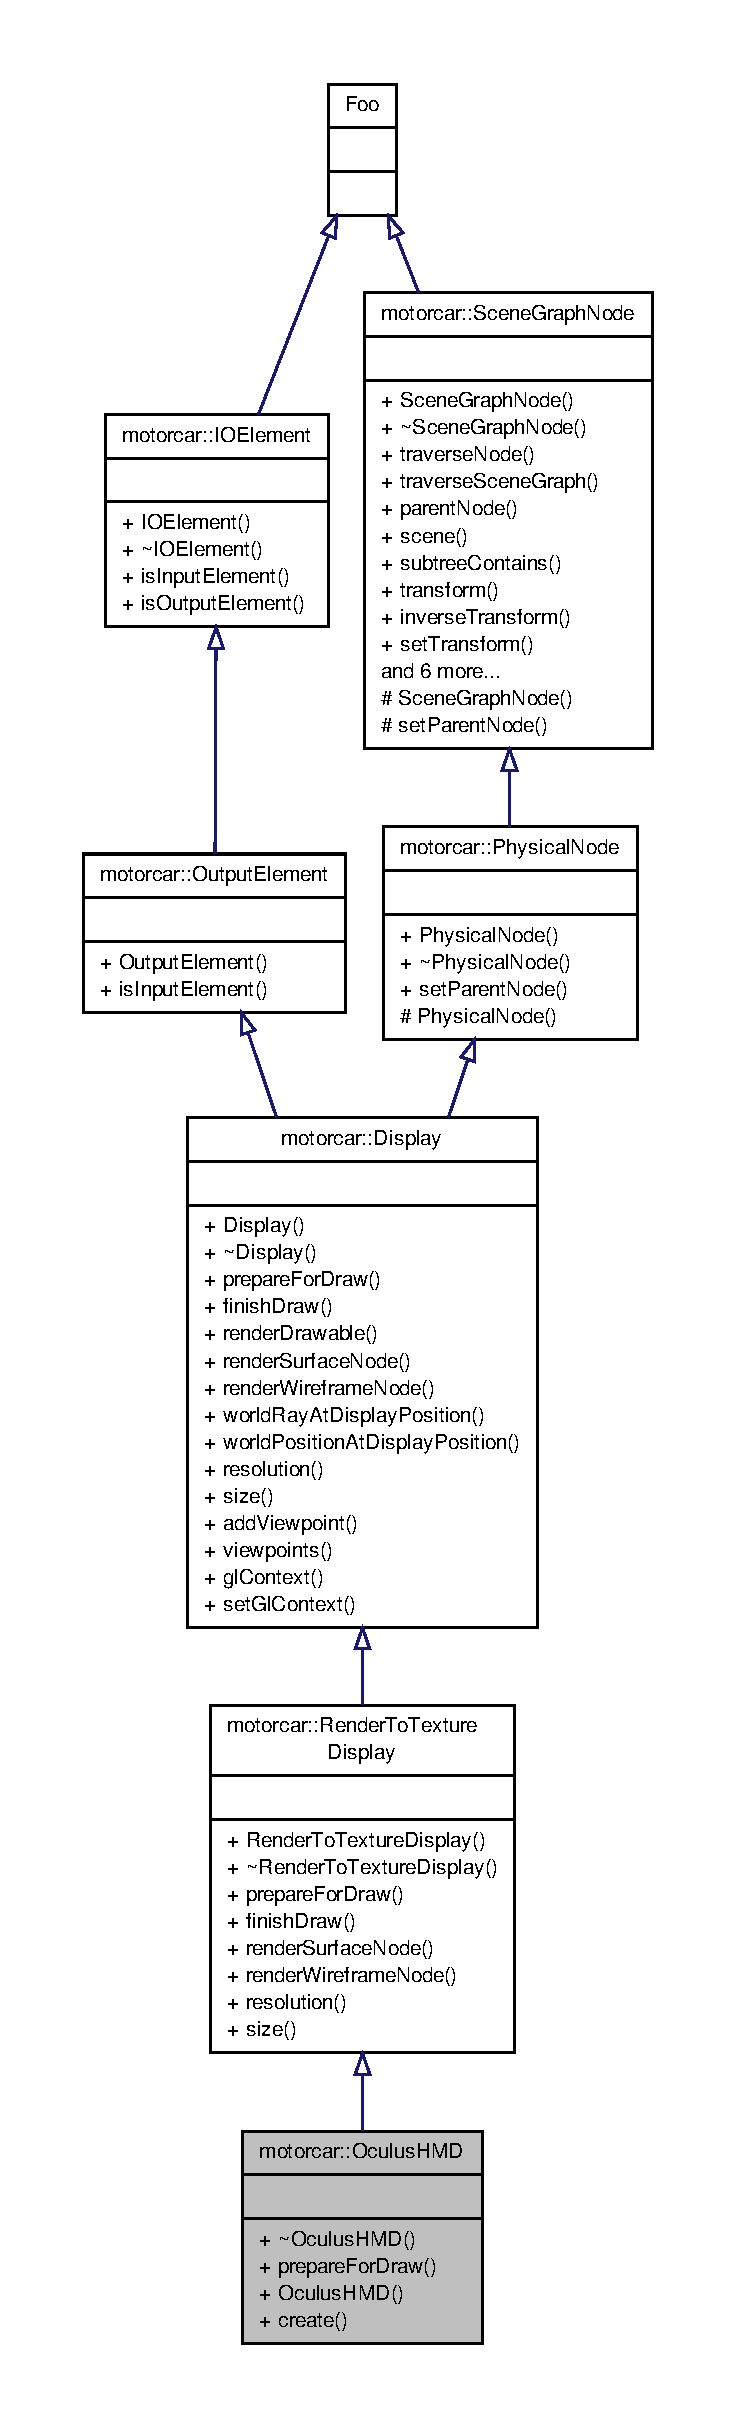
\includegraphics[width=332pt]{classmotorcar_1_1OculusHMD__coll__graph}
\end{center}
\end{figure}
\subsection*{Public Member Functions}
\begin{DoxyCompactItemize}
\item 
\hyperlink{classmotorcar_1_1OculusHMD_a69e38487ae0a51504663dd942fbb068e}{$\sim$\-Oculus\-H\-M\-D} ()
\item 
void \hyperlink{classmotorcar_1_1OculusHMD_ae9834ea50d728809532b7a48f7ed1738}{prepare\-For\-Draw} () override
\item 
\hyperlink{classmotorcar_1_1OculusHMD_a4f64cac13d749bf6d0cc9ca1f94297bb}{Oculus\-H\-M\-D} (O\-V\-R\-System $\ast$system, \hyperlink{classmotorcar_1_1Skeleton}{Skeleton} $\ast$skeleton, float scale, glm\-::vec4 distortion\-K, \hyperlink{classmotorcar_1_1OpenGLContext}{Open\-G\-L\-Context} $\ast$\hyperlink{classmotorcar_1_1Display_a884dd0b78dbecee82a33eb6d26a2a403}{gl\-Context}, glm\-::vec2 display\-Dimensions, \hyperlink{classmotorcar_1_1PhysicalNode}{Physical\-Node} $\ast$parent, const glm\-::mat4 \&\hyperlink{classmotorcar_1_1SceneGraphNode_ad96e79fdd739ac8223a3128003be391a}{transform})
\end{DoxyCompactItemize}
\subsection*{Static Public Member Functions}
\begin{DoxyCompactItemize}
\item 
static \hyperlink{classmotorcar_1_1OculusHMD}{Oculus\-H\-M\-D} $\ast$ \hyperlink{classmotorcar_1_1OculusHMD_aa77e2ef2bda8701075d5e669c95cc3ce}{create} (\hyperlink{classmotorcar_1_1OpenGLContext}{Open\-G\-L\-Context} $\ast$\hyperlink{classmotorcar_1_1Display_a884dd0b78dbecee82a33eb6d26a2a403}{gl\-Context}, \hyperlink{classmotorcar_1_1Skeleton}{Skeleton} $\ast$skeleton, \hyperlink{classmotorcar_1_1PhysicalNode}{Physical\-Node} $\ast$parent)
\end{DoxyCompactItemize}
\subsection*{Additional Inherited Members}


\subsection{Constructor \& Destructor Documentation}
\hypertarget{classmotorcar_1_1OculusHMD_a69e38487ae0a51504663dd942fbb068e}{\index{motorcar\-::\-Oculus\-H\-M\-D@{motorcar\-::\-Oculus\-H\-M\-D}!$\sim$\-Oculus\-H\-M\-D@{$\sim$\-Oculus\-H\-M\-D}}
\index{$\sim$\-Oculus\-H\-M\-D@{$\sim$\-Oculus\-H\-M\-D}!motorcar::OculusHMD@{motorcar\-::\-Oculus\-H\-M\-D}}
\subsubsection[{$\sim$\-Oculus\-H\-M\-D}]{\setlength{\rightskip}{0pt plus 5cm}Oculus\-H\-M\-D\-::$\sim$\-Oculus\-H\-M\-D (
\begin{DoxyParamCaption}
{}
\end{DoxyParamCaption}
)}}\label{classmotorcar_1_1OculusHMD_a69e38487ae0a51504663dd942fbb068e}
\hypertarget{classmotorcar_1_1OculusHMD_a4f64cac13d749bf6d0cc9ca1f94297bb}{\index{motorcar\-::\-Oculus\-H\-M\-D@{motorcar\-::\-Oculus\-H\-M\-D}!Oculus\-H\-M\-D@{Oculus\-H\-M\-D}}
\index{Oculus\-H\-M\-D@{Oculus\-H\-M\-D}!motorcar::OculusHMD@{motorcar\-::\-Oculus\-H\-M\-D}}
\subsubsection[{Oculus\-H\-M\-D}]{\setlength{\rightskip}{0pt plus 5cm}Oculus\-H\-M\-D\-::\-Oculus\-H\-M\-D (
\begin{DoxyParamCaption}
\item[{O\-V\-R\-System $\ast$}]{system, }
\item[{{\bf Skeleton} $\ast$}]{skeleton, }
\item[{float}]{scale, }
\item[{glm\-::vec4}]{distortion\-K, }
\item[{{\bf Open\-G\-L\-Context} $\ast$}]{gl\-Context, }
\item[{glm\-::vec2}]{display\-Dimensions, }
\item[{{\bf Physical\-Node} $\ast$}]{parent, }
\item[{const glm\-::mat4 \&}]{transform}
\end{DoxyParamCaption}
)}}\label{classmotorcar_1_1OculusHMD_a4f64cac13d749bf6d0cc9ca1f94297bb}


\subsection{Member Function Documentation}
\hypertarget{classmotorcar_1_1OculusHMD_aa77e2ef2bda8701075d5e669c95cc3ce}{\index{motorcar\-::\-Oculus\-H\-M\-D@{motorcar\-::\-Oculus\-H\-M\-D}!create@{create}}
\index{create@{create}!motorcar::OculusHMD@{motorcar\-::\-Oculus\-H\-M\-D}}
\subsubsection[{create}]{\setlength{\rightskip}{0pt plus 5cm}{\bf Oculus\-H\-M\-D} $\ast$ Oculus\-H\-M\-D\-::create (
\begin{DoxyParamCaption}
\item[{{\bf Open\-G\-L\-Context} $\ast$}]{gl\-Context, }
\item[{{\bf Skeleton} $\ast$}]{skeleton, }
\item[{{\bf Physical\-Node} $\ast$}]{parent}
\end{DoxyParamCaption}
)\hspace{0.3cm}{\ttfamily [static]}}}\label{classmotorcar_1_1OculusHMD_aa77e2ef2bda8701075d5e669c95cc3ce}
\hypertarget{classmotorcar_1_1OculusHMD_ae9834ea50d728809532b7a48f7ed1738}{\index{motorcar\-::\-Oculus\-H\-M\-D@{motorcar\-::\-Oculus\-H\-M\-D}!prepare\-For\-Draw@{prepare\-For\-Draw}}
\index{prepare\-For\-Draw@{prepare\-For\-Draw}!motorcar::OculusHMD@{motorcar\-::\-Oculus\-H\-M\-D}}
\subsubsection[{prepare\-For\-Draw}]{\setlength{\rightskip}{0pt plus 5cm}void Oculus\-H\-M\-D\-::prepare\-For\-Draw (
\begin{DoxyParamCaption}
{}
\end{DoxyParamCaption}
)\hspace{0.3cm}{\ttfamily [override]}, {\ttfamily [virtual]}}}\label{classmotorcar_1_1OculusHMD_ae9834ea50d728809532b7a48f7ed1738}


Reimplemented from \hyperlink{classmotorcar_1_1RenderToTextureDisplay_abdf6861fe69ada64fafd0a7713391bed}{motorcar\-::\-Render\-To\-Texture\-Display}.



The documentation for this class was generated from the following files\-:\begin{DoxyCompactItemize}
\item 
/media/dave/e89b5eb4-\/4b10-\/4edf-\/8ad5-\/0d046a46b978/dave/thesis/qtwayland-\/motorcar-\/compositor/motorcar/src/device/\hyperlink{oculushmd_8h}{oculushmd.\-h}\item 
/media/dave/e89b5eb4-\/4b10-\/4edf-\/8ad5-\/0d046a46b978/dave/thesis/qtwayland-\/motorcar-\/compositor/motorcar/src/device/\hyperlink{oculushmd_8cpp}{oculushmd.\-cpp}\end{DoxyCompactItemize}

\hypertarget{classmotorcar_1_1OpenGLContext}{\section{motorcar\-:\-:Open\-G\-L\-Context Class Reference}
\label{classmotorcar_1_1OpenGLContext}\index{motorcar\-::\-Open\-G\-L\-Context@{motorcar\-::\-Open\-G\-L\-Context}}
}


{\ttfamily \#include $<$openglcontext.\-h$>$}



Inheritance diagram for motorcar\-:\-:Open\-G\-L\-Context\-:
\nopagebreak
\begin{figure}[H]
\begin{center}
\leavevmode
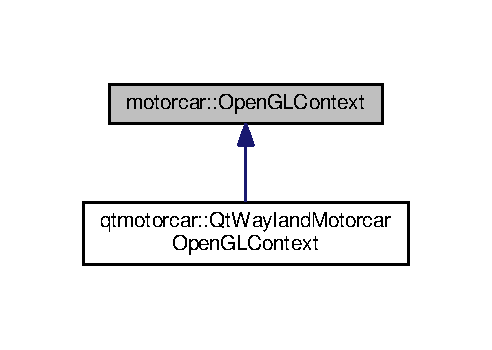
\includegraphics[width=236pt]{classmotorcar_1_1OpenGLContext__inherit__graph}
\end{center}
\end{figure}
\subsection*{Public Member Functions}
\begin{DoxyCompactItemize}
\item 
virtual \hyperlink{classmotorcar_1_1OpenGLContext_ac43c528ca955c030567c0654f171a680}{$\sim$\-Open\-G\-L\-Context} ()
\item 
virtual glm\-::ivec2 \hyperlink{classmotorcar_1_1OpenGLContext_a4a60274f217b9d71ff54ad60351b4127}{default\-Framebuffer\-Size} ()=0
\item 
virtual void \hyperlink{classmotorcar_1_1OpenGLContext_ae8b9c712092d01b69766469ab196ab80}{make\-Current} ()=0
\end{DoxyCompactItemize}


\subsection{Constructor \& Destructor Documentation}
\hypertarget{classmotorcar_1_1OpenGLContext_ac43c528ca955c030567c0654f171a680}{\index{motorcar\-::\-Open\-G\-L\-Context@{motorcar\-::\-Open\-G\-L\-Context}!$\sim$\-Open\-G\-L\-Context@{$\sim$\-Open\-G\-L\-Context}}
\index{$\sim$\-Open\-G\-L\-Context@{$\sim$\-Open\-G\-L\-Context}!motorcar::OpenGLContext@{motorcar\-::\-Open\-G\-L\-Context}}
\subsubsection[{$\sim$\-Open\-G\-L\-Context}]{\setlength{\rightskip}{0pt plus 5cm}virtual motorcar\-::\-Open\-G\-L\-Context\-::$\sim$\-Open\-G\-L\-Context (
\begin{DoxyParamCaption}
{}
\end{DoxyParamCaption}
)\hspace{0.3cm}{\ttfamily [inline]}, {\ttfamily [virtual]}}}\label{classmotorcar_1_1OpenGLContext_ac43c528ca955c030567c0654f171a680}


\subsection{Member Function Documentation}
\hypertarget{classmotorcar_1_1OpenGLContext_a4a60274f217b9d71ff54ad60351b4127}{\index{motorcar\-::\-Open\-G\-L\-Context@{motorcar\-::\-Open\-G\-L\-Context}!default\-Framebuffer\-Size@{default\-Framebuffer\-Size}}
\index{default\-Framebuffer\-Size@{default\-Framebuffer\-Size}!motorcar::OpenGLContext@{motorcar\-::\-Open\-G\-L\-Context}}
\subsubsection[{default\-Framebuffer\-Size}]{\setlength{\rightskip}{0pt plus 5cm}virtual glm\-::ivec2 motorcar\-::\-Open\-G\-L\-Context\-::default\-Framebuffer\-Size (
\begin{DoxyParamCaption}
{}
\end{DoxyParamCaption}
)\hspace{0.3cm}{\ttfamily [pure virtual]}}}\label{classmotorcar_1_1OpenGLContext_a4a60274f217b9d71ff54ad60351b4127}


Implemented in \hyperlink{classqtmotorcar_1_1QtWaylandMotorcarOpenGLContext_ab2a51af3b29de69f0a2d3d60d3bdbe82}{qtmotorcar\-::\-Qt\-Wayland\-Motorcar\-Open\-G\-L\-Context}.

\hypertarget{classmotorcar_1_1OpenGLContext_ae8b9c712092d01b69766469ab196ab80}{\index{motorcar\-::\-Open\-G\-L\-Context@{motorcar\-::\-Open\-G\-L\-Context}!make\-Current@{make\-Current}}
\index{make\-Current@{make\-Current}!motorcar::OpenGLContext@{motorcar\-::\-Open\-G\-L\-Context}}
\subsubsection[{make\-Current}]{\setlength{\rightskip}{0pt plus 5cm}virtual void motorcar\-::\-Open\-G\-L\-Context\-::make\-Current (
\begin{DoxyParamCaption}
{}
\end{DoxyParamCaption}
)\hspace{0.3cm}{\ttfamily [pure virtual]}}}\label{classmotorcar_1_1OpenGLContext_ae8b9c712092d01b69766469ab196ab80}


Implemented in \hyperlink{classqtmotorcar_1_1QtWaylandMotorcarOpenGLContext_ae5f00ad8258f7c03466ad114b64e250a}{qtmotorcar\-::\-Qt\-Wayland\-Motorcar\-Open\-G\-L\-Context}.



The documentation for this class was generated from the following file\-:\begin{DoxyCompactItemize}
\item 
/media/dave/e89b5eb4-\/4b10-\/4edf-\/8ad5-\/0d046a46b978/dave/thesis/qtwayland-\/motorcar-\/compositor/motorcar/src/gl/\hyperlink{openglcontext_8h}{openglcontext.\-h}\end{DoxyCompactItemize}

\hypertarget{classOpenGLData}{\section{Open\-G\-L\-Data Class Reference}
\label{classOpenGLData}\index{Open\-G\-L\-Data@{Open\-G\-L\-Data}}
}


{\ttfamily \#include $<$opengldata.\-h$>$}



Collaboration diagram for Open\-G\-L\-Data\-:
\nopagebreak
\begin{figure}[H]
\begin{center}
\leavevmode
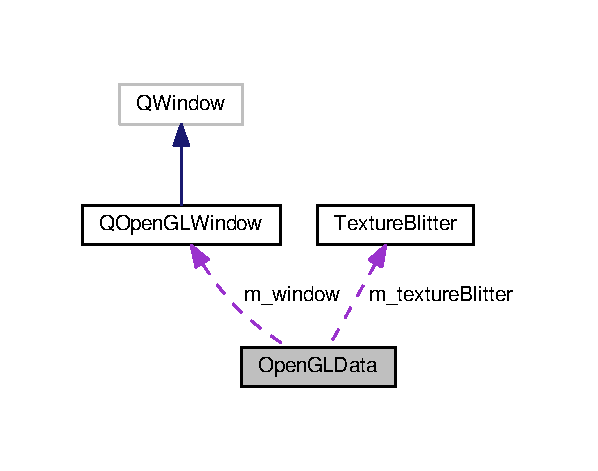
\includegraphics[width=287pt]{classOpenGLData__coll__graph}
\end{center}
\end{figure}
\subsection*{Public Member Functions}
\begin{DoxyCompactItemize}
\item 
\hyperlink{classOpenGLData_ae45b74d0a593e043189b8118e6abcb23}{Open\-G\-L\-Data} (\hyperlink{classQOpenGLWindow}{Q\-Open\-G\-L\-Window} $\ast$\hyperlink{structwindow}{window})
\item 
\hyperlink{classOpenGLData_a9241741339383a555a7189f472006a22}{$\sim$\-Open\-G\-L\-Data} ()
\item 
float \hyperlink{classOpenGLData_a8345c6c7bb79a3e48dfea00b786525c7}{ppcm} ()
\end{DoxyCompactItemize}
\subsection*{Public Attributes}
\begin{DoxyCompactItemize}
\item 
\hyperlink{classQOpenGLWindow}{Q\-Open\-G\-L\-Window} $\ast$ \hyperlink{classOpenGLData_ad4867a83945326a3523a1aa54bc1f016}{m\-\_\-window}
\item 
\hyperlink{classTextureBlitter}{Texture\-Blitter} $\ast$ \hyperlink{classOpenGLData_a7dce95e56b9349ca3a9d048ccc712748}{m\-\_\-texture\-Blitter}
\item 
Q\-Open\-G\-L\-Texture\-Cache $\ast$ \hyperlink{classOpenGLData_ac4c99b1032b6af264e738d02bdba4860}{m\-\_\-texture\-Cache}
\item 
G\-Luint \hyperlink{classOpenGLData_a0480263528e20beed53a1520272b296e}{m\-\_\-surface\-\_\-fbo}
\end{DoxyCompactItemize}


\subsection{Constructor \& Destructor Documentation}
\hypertarget{classOpenGLData_ae45b74d0a593e043189b8118e6abcb23}{\index{Open\-G\-L\-Data@{Open\-G\-L\-Data}!Open\-G\-L\-Data@{Open\-G\-L\-Data}}
\index{Open\-G\-L\-Data@{Open\-G\-L\-Data}!OpenGLData@{Open\-G\-L\-Data}}
\subsubsection[{Open\-G\-L\-Data}]{\setlength{\rightskip}{0pt plus 5cm}Open\-G\-L\-Data\-::\-Open\-G\-L\-Data (
\begin{DoxyParamCaption}
\item[{{\bf Q\-Open\-G\-L\-Window} $\ast$}]{window}
\end{DoxyParamCaption}
)}}\label{classOpenGLData_ae45b74d0a593e043189b8118e6abcb23}
\hypertarget{classOpenGLData_a9241741339383a555a7189f472006a22}{\index{Open\-G\-L\-Data@{Open\-G\-L\-Data}!$\sim$\-Open\-G\-L\-Data@{$\sim$\-Open\-G\-L\-Data}}
\index{$\sim$\-Open\-G\-L\-Data@{$\sim$\-Open\-G\-L\-Data}!OpenGLData@{Open\-G\-L\-Data}}
\subsubsection[{$\sim$\-Open\-G\-L\-Data}]{\setlength{\rightskip}{0pt plus 5cm}Open\-G\-L\-Data\-::$\sim$\-Open\-G\-L\-Data (
\begin{DoxyParamCaption}
{}
\end{DoxyParamCaption}
)}}\label{classOpenGLData_a9241741339383a555a7189f472006a22}


\subsection{Member Function Documentation}
\hypertarget{classOpenGLData_a8345c6c7bb79a3e48dfea00b786525c7}{\index{Open\-G\-L\-Data@{Open\-G\-L\-Data}!ppcm@{ppcm}}
\index{ppcm@{ppcm}!OpenGLData@{Open\-G\-L\-Data}}
\subsubsection[{ppcm}]{\setlength{\rightskip}{0pt plus 5cm}float Open\-G\-L\-Data\-::ppcm (
\begin{DoxyParamCaption}
{}
\end{DoxyParamCaption}
)}}\label{classOpenGLData_a8345c6c7bb79a3e48dfea00b786525c7}


\subsection{Member Data Documentation}
\hypertarget{classOpenGLData_a0480263528e20beed53a1520272b296e}{\index{Open\-G\-L\-Data@{Open\-G\-L\-Data}!m\-\_\-surface\-\_\-fbo@{m\-\_\-surface\-\_\-fbo}}
\index{m\-\_\-surface\-\_\-fbo@{m\-\_\-surface\-\_\-fbo}!OpenGLData@{Open\-G\-L\-Data}}
\subsubsection[{m\-\_\-surface\-\_\-fbo}]{\setlength{\rightskip}{0pt plus 5cm}G\-Luint Open\-G\-L\-Data\-::m\-\_\-surface\-\_\-fbo}}\label{classOpenGLData_a0480263528e20beed53a1520272b296e}
\hypertarget{classOpenGLData_a7dce95e56b9349ca3a9d048ccc712748}{\index{Open\-G\-L\-Data@{Open\-G\-L\-Data}!m\-\_\-texture\-Blitter@{m\-\_\-texture\-Blitter}}
\index{m\-\_\-texture\-Blitter@{m\-\_\-texture\-Blitter}!OpenGLData@{Open\-G\-L\-Data}}
\subsubsection[{m\-\_\-texture\-Blitter}]{\setlength{\rightskip}{0pt plus 5cm}{\bf Texture\-Blitter}$\ast$ Open\-G\-L\-Data\-::m\-\_\-texture\-Blitter}}\label{classOpenGLData_a7dce95e56b9349ca3a9d048ccc712748}
\hypertarget{classOpenGLData_ac4c99b1032b6af264e738d02bdba4860}{\index{Open\-G\-L\-Data@{Open\-G\-L\-Data}!m\-\_\-texture\-Cache@{m\-\_\-texture\-Cache}}
\index{m\-\_\-texture\-Cache@{m\-\_\-texture\-Cache}!OpenGLData@{Open\-G\-L\-Data}}
\subsubsection[{m\-\_\-texture\-Cache}]{\setlength{\rightskip}{0pt plus 5cm}Q\-Open\-G\-L\-Texture\-Cache$\ast$ Open\-G\-L\-Data\-::m\-\_\-texture\-Cache}}\label{classOpenGLData_ac4c99b1032b6af264e738d02bdba4860}
\hypertarget{classOpenGLData_ad4867a83945326a3523a1aa54bc1f016}{\index{Open\-G\-L\-Data@{Open\-G\-L\-Data}!m\-\_\-window@{m\-\_\-window}}
\index{m\-\_\-window@{m\-\_\-window}!OpenGLData@{Open\-G\-L\-Data}}
\subsubsection[{m\-\_\-window}]{\setlength{\rightskip}{0pt plus 5cm}{\bf Q\-Open\-G\-L\-Window}$\ast$ Open\-G\-L\-Data\-::m\-\_\-window}}\label{classOpenGLData_ad4867a83945326a3523a1aa54bc1f016}


The documentation for this class was generated from the following files\-:\begin{DoxyCompactItemize}
\item 
/media/dave/e89b5eb4-\/4b10-\/4edf-\/8ad5-\/0d046a46b978/dave/thesis/qtwayland-\/motorcar-\/compositor/qt/src/\hyperlink{opengldata_8h}{opengldata.\-h}\item 
/media/dave/e89b5eb4-\/4b10-\/4edf-\/8ad5-\/0d046a46b978/dave/thesis/qtwayland-\/motorcar-\/compositor/qt/src/\hyperlink{opengldata_8cpp}{opengldata.\-cpp}\end{DoxyCompactItemize}

\hypertarget{classmotorcar_1_1OpenGLShader}{\section{motorcar\-:\-:Open\-G\-L\-Shader Class Reference}
\label{classmotorcar_1_1OpenGLShader}\index{motorcar\-::\-Open\-G\-L\-Shader@{motorcar\-::\-Open\-G\-L\-Shader}}
}


{\ttfamily \#include $<$openglshader.\-h$>$}

\subsection*{Public Member Functions}
\begin{DoxyCompactItemize}
\item 
\hyperlink{classmotorcar_1_1OpenGLShader_a0074dbe42bf05b0e0631a1420b767391}{Open\-G\-L\-Shader} (std\-::string vertex\-Shader\-File\-Name, std\-::string fragment\-Shader\-File\-Name)
\item 
G\-Luint \hyperlink{classmotorcar_1_1OpenGLShader_a4b252b4c961c266261715e4c3c8f66d4}{handle} () const 
\end{DoxyCompactItemize}


\subsection{Constructor \& Destructor Documentation}
\hypertarget{classmotorcar_1_1OpenGLShader_a0074dbe42bf05b0e0631a1420b767391}{\index{motorcar\-::\-Open\-G\-L\-Shader@{motorcar\-::\-Open\-G\-L\-Shader}!Open\-G\-L\-Shader@{Open\-G\-L\-Shader}}
\index{Open\-G\-L\-Shader@{Open\-G\-L\-Shader}!motorcar::OpenGLShader@{motorcar\-::\-Open\-G\-L\-Shader}}
\subsubsection[{Open\-G\-L\-Shader}]{\setlength{\rightskip}{0pt plus 5cm}Open\-G\-L\-Shader\-::\-Open\-G\-L\-Shader (
\begin{DoxyParamCaption}
\item[{std\-::string}]{vertex\-Shader\-File\-Name, }
\item[{std\-::string}]{fragment\-Shader\-File\-Name}
\end{DoxyParamCaption}
)}}\label{classmotorcar_1_1OpenGLShader_a0074dbe42bf05b0e0631a1420b767391}


\subsection{Member Function Documentation}
\hypertarget{classmotorcar_1_1OpenGLShader_a4b252b4c961c266261715e4c3c8f66d4}{\index{motorcar\-::\-Open\-G\-L\-Shader@{motorcar\-::\-Open\-G\-L\-Shader}!handle@{handle}}
\index{handle@{handle}!motorcar::OpenGLShader@{motorcar\-::\-Open\-G\-L\-Shader}}
\subsubsection[{handle}]{\setlength{\rightskip}{0pt plus 5cm}G\-Luint Open\-G\-L\-Shader\-::handle (
\begin{DoxyParamCaption}
{}
\end{DoxyParamCaption}
) const}}\label{classmotorcar_1_1OpenGLShader_a4b252b4c961c266261715e4c3c8f66d4}


The documentation for this class was generated from the following files\-:\begin{DoxyCompactItemize}
\item 
/home/dave/thesis/motorcar/src/compositor/gl/\hyperlink{openglshader_8h}{openglshader.\-h}\item 
/home/dave/thesis/motorcar/src/compositor/gl/\hyperlink{openglshader_8cpp}{openglshader.\-cpp}\end{DoxyCompactItemize}

\hypertarget{classmotorcar_1_1PhysicalNode}{\section{motorcar\-:\-:Physical\-Node Class Reference}
\label{classmotorcar_1_1PhysicalNode}\index{motorcar\-::\-Physical\-Node@{motorcar\-::\-Physical\-Node}}
}


{\ttfamily \#include $<$physicalnode.\-h$>$}



Inheritance diagram for motorcar\-:\-:Physical\-Node\-:
\nopagebreak
\begin{figure}[H]
\begin{center}
\leavevmode
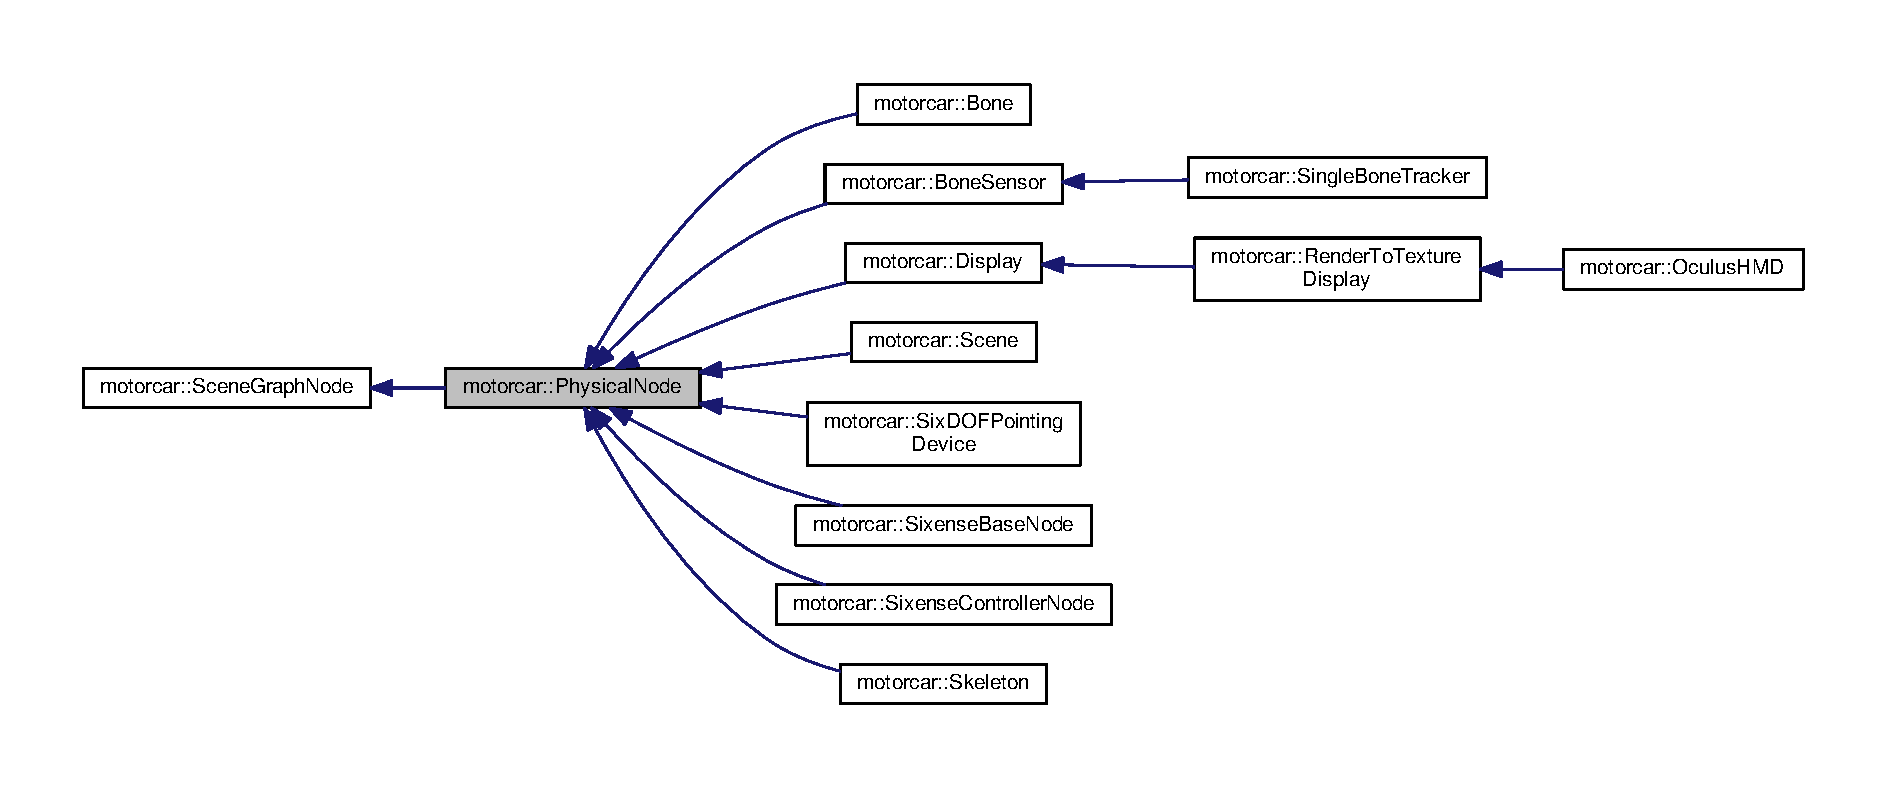
\includegraphics[width=350pt]{classmotorcar_1_1PhysicalNode__inherit__graph}
\end{center}
\end{figure}


Collaboration diagram for motorcar\-:\-:Physical\-Node\-:
\nopagebreak
\begin{figure}[H]
\begin{center}
\leavevmode
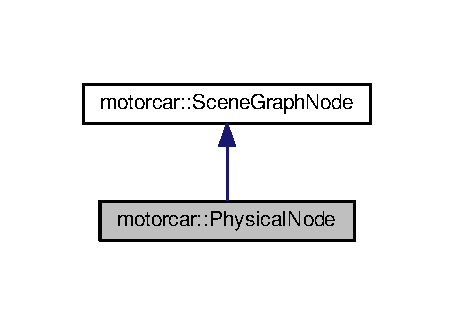
\includegraphics[width=218pt]{classmotorcar_1_1PhysicalNode__coll__graph}
\end{center}
\end{figure}
\subsection*{Public Member Functions}
\begin{DoxyCompactItemize}
\item 
\hyperlink{classmotorcar_1_1PhysicalNode_a91ba5f3ead25d072f128375369b75fe0}{Physical\-Node} (\hyperlink{classmotorcar_1_1PhysicalNode}{Physical\-Node} $\ast$parent, const glm\-::mat4 \&\hyperlink{classmotorcar_1_1SceneGraphNode_ad96e79fdd739ac8223a3128003be391a}{transform}=glm\-::mat4())
\item 
virtual \hyperlink{classmotorcar_1_1PhysicalNode_aa132dbe84a01971eb4e149852a1b52f1}{$\sim$\-Physical\-Node} ()
\item 
void \hyperlink{classmotorcar_1_1PhysicalNode_aadcd6c81c0f8b2f57e6bebe9100d0690}{set\-Parent\-Node} (\hyperlink{classmotorcar_1_1PhysicalNode}{Physical\-Node} $\ast$parent)
\end{DoxyCompactItemize}
\subsection*{Protected Member Functions}
\begin{DoxyCompactItemize}
\item 
\hyperlink{classmotorcar_1_1PhysicalNode_a8194d6949b0886071bda80fb314aabde}{Physical\-Node} ()
\end{DoxyCompactItemize}


\subsection{Constructor \& Destructor Documentation}
\hypertarget{classmotorcar_1_1PhysicalNode_a91ba5f3ead25d072f128375369b75fe0}{\index{motorcar\-::\-Physical\-Node@{motorcar\-::\-Physical\-Node}!Physical\-Node@{Physical\-Node}}
\index{Physical\-Node@{Physical\-Node}!motorcar::PhysicalNode@{motorcar\-::\-Physical\-Node}}
\subsubsection[{Physical\-Node}]{\setlength{\rightskip}{0pt plus 5cm}Physical\-Node\-::\-Physical\-Node (
\begin{DoxyParamCaption}
\item[{{\bf Physical\-Node} $\ast$}]{parent, }
\item[{const glm\-::mat4 \&}]{transform = {\ttfamily glm\-:\-:mat4()}}
\end{DoxyParamCaption}
)}}\label{classmotorcar_1_1PhysicalNode_a91ba5f3ead25d072f128375369b75fe0}
\hypertarget{classmotorcar_1_1PhysicalNode_aa132dbe84a01971eb4e149852a1b52f1}{\index{motorcar\-::\-Physical\-Node@{motorcar\-::\-Physical\-Node}!$\sim$\-Physical\-Node@{$\sim$\-Physical\-Node}}
\index{$\sim$\-Physical\-Node@{$\sim$\-Physical\-Node}!motorcar::PhysicalNode@{motorcar\-::\-Physical\-Node}}
\subsubsection[{$\sim$\-Physical\-Node}]{\setlength{\rightskip}{0pt plus 5cm}virtual motorcar\-::\-Physical\-Node\-::$\sim$\-Physical\-Node (
\begin{DoxyParamCaption}
{}
\end{DoxyParamCaption}
)\hspace{0.3cm}{\ttfamily [inline]}, {\ttfamily [virtual]}}}\label{classmotorcar_1_1PhysicalNode_aa132dbe84a01971eb4e149852a1b52f1}
\hypertarget{classmotorcar_1_1PhysicalNode_a8194d6949b0886071bda80fb314aabde}{\index{motorcar\-::\-Physical\-Node@{motorcar\-::\-Physical\-Node}!Physical\-Node@{Physical\-Node}}
\index{Physical\-Node@{Physical\-Node}!motorcar::PhysicalNode@{motorcar\-::\-Physical\-Node}}
\subsubsection[{Physical\-Node}]{\setlength{\rightskip}{0pt plus 5cm}Physical\-Node\-::\-Physical\-Node (
\begin{DoxyParamCaption}
{}
\end{DoxyParamCaption}
)\hspace{0.3cm}{\ttfamily [protected]}}}\label{classmotorcar_1_1PhysicalNode_a8194d6949b0886071bda80fb314aabde}


\subsection{Member Function Documentation}
\hypertarget{classmotorcar_1_1PhysicalNode_aadcd6c81c0f8b2f57e6bebe9100d0690}{\index{motorcar\-::\-Physical\-Node@{motorcar\-::\-Physical\-Node}!set\-Parent\-Node@{set\-Parent\-Node}}
\index{set\-Parent\-Node@{set\-Parent\-Node}!motorcar::PhysicalNode@{motorcar\-::\-Physical\-Node}}
\subsubsection[{set\-Parent\-Node}]{\setlength{\rightskip}{0pt plus 5cm}void Physical\-Node\-::set\-Parent\-Node (
\begin{DoxyParamCaption}
\item[{{\bf Physical\-Node} $\ast$}]{parent}
\end{DoxyParamCaption}
)}}\label{classmotorcar_1_1PhysicalNode_aadcd6c81c0f8b2f57e6bebe9100d0690}


The documentation for this class was generated from the following files\-:\begin{DoxyCompactItemize}
\item 
/home/dave/thesis/qtwayland-\/motorcar-\/compositor/motorcar/src/scenegraph/\hyperlink{physicalnode_8h}{physicalnode.\-h}\item 
/home/dave/thesis/qtwayland-\/motorcar-\/compositor/motorcar/src/scenegraph/\hyperlink{physicalnode_8cpp}{physicalnode.\-cpp}\end{DoxyCompactItemize}

\hypertarget{structmotorcar_1_1Geometry_1_1Plane}{\section{motorcar\-:\-:Geometry\-:\-:Plane Struct Reference}
\label{structmotorcar_1_1Geometry_1_1Plane}\index{motorcar\-::\-Geometry\-::\-Plane@{motorcar\-::\-Geometry\-::\-Plane}}
}


{\ttfamily \#include $<$geometry.\-h$>$}

\subsection*{Public Member Functions}
\begin{DoxyCompactItemize}
\item 
\hyperlink{structmotorcar_1_1Geometry_1_1Plane_aa50a62c6e979384b4026a1ba81a29c19}{Plane} (glm\-::vec3 \hyperlink{structmotorcar_1_1Geometry_1_1Plane_ad1aa2ffa451147b0fe911f5b78c10500}{p}, glm\-::vec3 \hyperlink{structmotorcar_1_1Geometry_1_1Plane_adc343be1d51473ca22505d7427a7631c}{n})
\item 
float \hyperlink{structmotorcar_1_1Geometry_1_1Plane_a108d18bf80259951130d1b2b7e8bf8ce}{intersect} (\hyperlink{structmotorcar_1_1Geometry_1_1Ray}{Ray} r)
\end{DoxyCompactItemize}
\subsection*{Public Attributes}
\begin{DoxyCompactItemize}
\item 
glm\-::vec3 \hyperlink{structmotorcar_1_1Geometry_1_1Plane_ad1aa2ffa451147b0fe911f5b78c10500}{p}
\item 
glm\-::vec3 \hyperlink{structmotorcar_1_1Geometry_1_1Plane_adc343be1d51473ca22505d7427a7631c}{n}
\end{DoxyCompactItemize}


\subsection{Constructor \& Destructor Documentation}
\hypertarget{structmotorcar_1_1Geometry_1_1Plane_aa50a62c6e979384b4026a1ba81a29c19}{\index{motorcar\-::\-Geometry\-::\-Plane@{motorcar\-::\-Geometry\-::\-Plane}!Plane@{Plane}}
\index{Plane@{Plane}!motorcar::Geometry::Plane@{motorcar\-::\-Geometry\-::\-Plane}}
\subsubsection[{Plane}]{\setlength{\rightskip}{0pt plus 5cm}Geometry\-::\-Plane\-::\-Plane (
\begin{DoxyParamCaption}
\item[{glm\-::vec3}]{p, }
\item[{glm\-::vec3}]{n}
\end{DoxyParamCaption}
)}}\label{structmotorcar_1_1Geometry_1_1Plane_aa50a62c6e979384b4026a1ba81a29c19}


\subsection{Member Function Documentation}
\hypertarget{structmotorcar_1_1Geometry_1_1Plane_a108d18bf80259951130d1b2b7e8bf8ce}{\index{motorcar\-::\-Geometry\-::\-Plane@{motorcar\-::\-Geometry\-::\-Plane}!intersect@{intersect}}
\index{intersect@{intersect}!motorcar::Geometry::Plane@{motorcar\-::\-Geometry\-::\-Plane}}
\subsubsection[{intersect}]{\setlength{\rightskip}{0pt plus 5cm}float Geometry\-::\-Plane\-::intersect (
\begin{DoxyParamCaption}
\item[{{\bf Geometry\-::\-Ray}}]{r}
\end{DoxyParamCaption}
)}}\label{structmotorcar_1_1Geometry_1_1Plane_a108d18bf80259951130d1b2b7e8bf8ce}


\subsection{Member Data Documentation}
\hypertarget{structmotorcar_1_1Geometry_1_1Plane_adc343be1d51473ca22505d7427a7631c}{\index{motorcar\-::\-Geometry\-::\-Plane@{motorcar\-::\-Geometry\-::\-Plane}!n@{n}}
\index{n@{n}!motorcar::Geometry::Plane@{motorcar\-::\-Geometry\-::\-Plane}}
\subsubsection[{n}]{\setlength{\rightskip}{0pt plus 5cm}glm\-::vec3 motorcar\-::\-Geometry\-::\-Plane\-::n}}\label{structmotorcar_1_1Geometry_1_1Plane_adc343be1d51473ca22505d7427a7631c}
\hypertarget{structmotorcar_1_1Geometry_1_1Plane_ad1aa2ffa451147b0fe911f5b78c10500}{\index{motorcar\-::\-Geometry\-::\-Plane@{motorcar\-::\-Geometry\-::\-Plane}!p@{p}}
\index{p@{p}!motorcar::Geometry::Plane@{motorcar\-::\-Geometry\-::\-Plane}}
\subsubsection[{p}]{\setlength{\rightskip}{0pt plus 5cm}glm\-::vec3 motorcar\-::\-Geometry\-::\-Plane\-::p}}\label{structmotorcar_1_1Geometry_1_1Plane_ad1aa2ffa451147b0fe911f5b78c10500}


The documentation for this struct was generated from the following files\-:\begin{DoxyCompactItemize}
\item 
/home/dave/thesis/motorcar/src/compositor/\hyperlink{geometry_8h}{geometry.\-h}\item 
/home/dave/thesis/motorcar/src/compositor/\hyperlink{geometry_8cpp}{geometry.\-cpp}\end{DoxyCompactItemize}

\hypertarget{classmotorcar_1_1Pointer}{\section{motorcar\-:\-:Pointer Class Reference}
\label{classmotorcar_1_1Pointer}\index{motorcar\-::\-Pointer@{motorcar\-::\-Pointer}}
}


{\ttfamily \#include $<$pointer.\-h$>$}

\subsection*{Public Member Functions}
\begin{DoxyCompactItemize}
\item 
\hyperlink{classmotorcar_1_1Pointer_abfbd5397af7d39289d7f3d7eb2db734d}{Pointer} (\hyperlink{classmotorcar_1_1Seat}{Seat} $\ast$seat)
\item 
glm\-::vec2 \hyperlink{classmotorcar_1_1Pointer_a19f25225f16b8f4f2289e008bc75d957}{local\-Positon} () const 
\item 
void \hyperlink{classmotorcar_1_1Pointer_abe379b3238e6fe31b959b8affdc00ea2}{set\-Local\-Positon} (const glm\-::vec2 \&\hyperlink{classmotorcar_1_1Pointer_a19f25225f16b8f4f2289e008bc75d957}{local\-Positon})
\item 
\hyperlink{classmotorcar_1_1WaylandSurface}{Wayland\-Surface} $\ast$ \hyperlink{classmotorcar_1_1Pointer_a6b93402a87e64c673fef44d0102be63b}{focus} () const 
\item 
void \hyperlink{classmotorcar_1_1Pointer_afea4df13d7805e699c523c7aaaf30c4c}{set\-Focus} (\hyperlink{classmotorcar_1_1WaylandSurface}{Wayland\-Surface} $\ast$\hyperlink{classmotorcar_1_1Pointer_a6b93402a87e64c673fef44d0102be63b}{focus})
\item 
\hyperlink{classmotorcar_1_1WaylandSurfaceNode}{Wayland\-Surface\-Node} $\ast$ \hyperlink{classmotorcar_1_1Pointer_a97586b3be93be794761ca2b97864fc9e}{cursor\-Node} () const 
\item 
void \hyperlink{classmotorcar_1_1Pointer_a0bb8c2cfc6523155cc4b3f37487937fa}{set\-Cursor\-Node} (\hyperlink{classmotorcar_1_1WaylandSurfaceNode}{Wayland\-Surface\-Node} $\ast$\hyperlink{classmotorcar_1_1Pointer_a97586b3be93be794761ca2b97864fc9e}{cursor\-Node})
\item 
glm\-::ivec2 \hyperlink{classmotorcar_1_1Pointer_ae847516f0a34b7018bf0cdbd26a7d831}{cursor\-Hotspot} () const 
\item 
void \hyperlink{classmotorcar_1_1Pointer_ae8f489d37a9520e41d8f5162cff3992e}{set\-Cursor\-Hotspot} (const glm\-::ivec2 \&\hyperlink{classmotorcar_1_1Pointer_ae847516f0a34b7018bf0cdbd26a7d831}{cursor\-Hotspot})
\end{DoxyCompactItemize}


\subsection{Constructor \& Destructor Documentation}
\hypertarget{classmotorcar_1_1Pointer_abfbd5397af7d39289d7f3d7eb2db734d}{\index{motorcar\-::\-Pointer@{motorcar\-::\-Pointer}!Pointer@{Pointer}}
\index{Pointer@{Pointer}!motorcar::Pointer@{motorcar\-::\-Pointer}}
\subsubsection[{Pointer}]{\setlength{\rightskip}{0pt plus 5cm}Pointer\-::\-Pointer (
\begin{DoxyParamCaption}
\item[{{\bf Seat} $\ast$}]{seat}
\end{DoxyParamCaption}
)}}\label{classmotorcar_1_1Pointer_abfbd5397af7d39289d7f3d7eb2db734d}


\subsection{Member Function Documentation}
\hypertarget{classmotorcar_1_1Pointer_ae847516f0a34b7018bf0cdbd26a7d831}{\index{motorcar\-::\-Pointer@{motorcar\-::\-Pointer}!cursor\-Hotspot@{cursor\-Hotspot}}
\index{cursor\-Hotspot@{cursor\-Hotspot}!motorcar::Pointer@{motorcar\-::\-Pointer}}
\subsubsection[{cursor\-Hotspot}]{\setlength{\rightskip}{0pt plus 5cm}glm\-::ivec2 Pointer\-::cursor\-Hotspot (
\begin{DoxyParamCaption}
{}
\end{DoxyParamCaption}
) const}}\label{classmotorcar_1_1Pointer_ae847516f0a34b7018bf0cdbd26a7d831}
\hypertarget{classmotorcar_1_1Pointer_a97586b3be93be794761ca2b97864fc9e}{\index{motorcar\-::\-Pointer@{motorcar\-::\-Pointer}!cursor\-Node@{cursor\-Node}}
\index{cursor\-Node@{cursor\-Node}!motorcar::Pointer@{motorcar\-::\-Pointer}}
\subsubsection[{cursor\-Node}]{\setlength{\rightskip}{0pt plus 5cm}{\bf Wayland\-Surface\-Node} $\ast$ Pointer\-::cursor\-Node (
\begin{DoxyParamCaption}
{}
\end{DoxyParamCaption}
) const}}\label{classmotorcar_1_1Pointer_a97586b3be93be794761ca2b97864fc9e}
\hypertarget{classmotorcar_1_1Pointer_a6b93402a87e64c673fef44d0102be63b}{\index{motorcar\-::\-Pointer@{motorcar\-::\-Pointer}!focus@{focus}}
\index{focus@{focus}!motorcar::Pointer@{motorcar\-::\-Pointer}}
\subsubsection[{focus}]{\setlength{\rightskip}{0pt plus 5cm}{\bf Wayland\-Surface} $\ast$ Pointer\-::focus (
\begin{DoxyParamCaption}
{}
\end{DoxyParamCaption}
) const}}\label{classmotorcar_1_1Pointer_a6b93402a87e64c673fef44d0102be63b}
\hypertarget{classmotorcar_1_1Pointer_a19f25225f16b8f4f2289e008bc75d957}{\index{motorcar\-::\-Pointer@{motorcar\-::\-Pointer}!local\-Positon@{local\-Positon}}
\index{local\-Positon@{local\-Positon}!motorcar::Pointer@{motorcar\-::\-Pointer}}
\subsubsection[{local\-Positon}]{\setlength{\rightskip}{0pt plus 5cm}glm\-::vec2 Pointer\-::local\-Positon (
\begin{DoxyParamCaption}
{}
\end{DoxyParamCaption}
) const}}\label{classmotorcar_1_1Pointer_a19f25225f16b8f4f2289e008bc75d957}
\hypertarget{classmotorcar_1_1Pointer_ae8f489d37a9520e41d8f5162cff3992e}{\index{motorcar\-::\-Pointer@{motorcar\-::\-Pointer}!set\-Cursor\-Hotspot@{set\-Cursor\-Hotspot}}
\index{set\-Cursor\-Hotspot@{set\-Cursor\-Hotspot}!motorcar::Pointer@{motorcar\-::\-Pointer}}
\subsubsection[{set\-Cursor\-Hotspot}]{\setlength{\rightskip}{0pt plus 5cm}void Pointer\-::set\-Cursor\-Hotspot (
\begin{DoxyParamCaption}
\item[{const glm\-::ivec2 \&}]{cursor\-Hotspot}
\end{DoxyParamCaption}
)}}\label{classmotorcar_1_1Pointer_ae8f489d37a9520e41d8f5162cff3992e}
\hypertarget{classmotorcar_1_1Pointer_a0bb8c2cfc6523155cc4b3f37487937fa}{\index{motorcar\-::\-Pointer@{motorcar\-::\-Pointer}!set\-Cursor\-Node@{set\-Cursor\-Node}}
\index{set\-Cursor\-Node@{set\-Cursor\-Node}!motorcar::Pointer@{motorcar\-::\-Pointer}}
\subsubsection[{set\-Cursor\-Node}]{\setlength{\rightskip}{0pt plus 5cm}void Pointer\-::set\-Cursor\-Node (
\begin{DoxyParamCaption}
\item[{{\bf Wayland\-Surface\-Node} $\ast$}]{cursor\-Node}
\end{DoxyParamCaption}
)}}\label{classmotorcar_1_1Pointer_a0bb8c2cfc6523155cc4b3f37487937fa}
\hypertarget{classmotorcar_1_1Pointer_afea4df13d7805e699c523c7aaaf30c4c}{\index{motorcar\-::\-Pointer@{motorcar\-::\-Pointer}!set\-Focus@{set\-Focus}}
\index{set\-Focus@{set\-Focus}!motorcar::Pointer@{motorcar\-::\-Pointer}}
\subsubsection[{set\-Focus}]{\setlength{\rightskip}{0pt plus 5cm}void Pointer\-::set\-Focus (
\begin{DoxyParamCaption}
\item[{{\bf Wayland\-Surface} $\ast$}]{focus}
\end{DoxyParamCaption}
)}}\label{classmotorcar_1_1Pointer_afea4df13d7805e699c523c7aaaf30c4c}
\hypertarget{classmotorcar_1_1Pointer_abe379b3238e6fe31b959b8affdc00ea2}{\index{motorcar\-::\-Pointer@{motorcar\-::\-Pointer}!set\-Local\-Positon@{set\-Local\-Positon}}
\index{set\-Local\-Positon@{set\-Local\-Positon}!motorcar::Pointer@{motorcar\-::\-Pointer}}
\subsubsection[{set\-Local\-Positon}]{\setlength{\rightskip}{0pt plus 5cm}void Pointer\-::set\-Local\-Positon (
\begin{DoxyParamCaption}
\item[{const glm\-::vec2 \&}]{local\-Positon}
\end{DoxyParamCaption}
)}}\label{classmotorcar_1_1Pointer_abe379b3238e6fe31b959b8affdc00ea2}


The documentation for this class was generated from the following files\-:\begin{DoxyCompactItemize}
\item 
/home/dave/thesis/motorcar/src/compositor/wayland/input/\hyperlink{pointer_8h}{pointer.\-h}\item 
/home/dave/thesis/motorcar/src/compositor/wayland/input/\hyperlink{pointer_8cpp}{pointer.\-cpp}\end{DoxyCompactItemize}

\hypertarget{classQOpenGLWindow}{\section{Q\-Open\-G\-L\-Window Class Reference}
\label{classQOpenGLWindow}\index{Q\-Open\-G\-L\-Window@{Q\-Open\-G\-L\-Window}}
}


{\ttfamily \#include $<$qopenglwindow.\-h$>$}



Inheritance diagram for Q\-Open\-G\-L\-Window\-:
\nopagebreak
\begin{figure}[H]
\begin{center}
\leavevmode
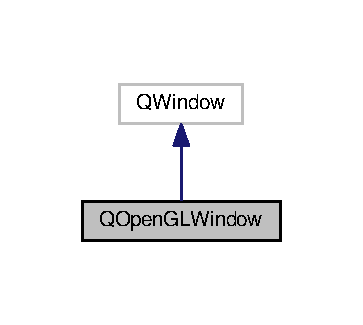
\includegraphics[width=174pt]{classQOpenGLWindow__inherit__graph}
\end{center}
\end{figure}


Collaboration diagram for Q\-Open\-G\-L\-Window\-:
\nopagebreak
\begin{figure}[H]
\begin{center}
\leavevmode
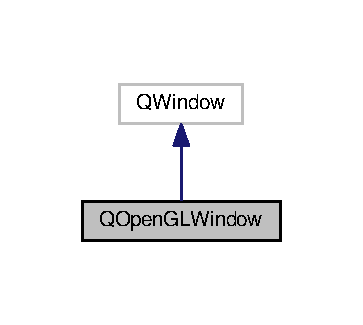
\includegraphics[width=174pt]{classQOpenGLWindow__coll__graph}
\end{center}
\end{figure}
\subsection*{Public Member Functions}
\begin{DoxyCompactItemize}
\item 
\hyperlink{classQOpenGLWindow_a45d1b287e72113aaa653e8e937ebdfd6}{Q\-Open\-G\-L\-Window} (const Q\-Surface\-Format \&format, const Q\-Rect \&\hyperlink{structgeometry}{geometry})
\item 
Q\-Open\-G\-L\-Context $\ast$ \hyperlink{classQOpenGLWindow_ac50866b8a1e723bccea33df6c5a3d1b3}{context} ()
\item 
bool \hyperlink{classQOpenGLWindow_af7602ba08fd50ee8fb9ccbed2d121404}{make\-Current} ()
\item 
void \hyperlink{classQOpenGLWindow_ae8b962ff83b505543adfcd52f4fb203b}{swap\-Buffers} ()
\end{DoxyCompactItemize}
\subsection*{Protected Member Functions}
\begin{DoxyCompactItemize}
\item 
void \hyperlink{classQOpenGLWindow_a60ae6ea64e5efc1a21dea97429ebb838}{touch\-Event} (Q\-Touch\-Event $\ast$event)
\end{DoxyCompactItemize}


\subsection{Constructor \& Destructor Documentation}
\hypertarget{classQOpenGLWindow_a45d1b287e72113aaa653e8e937ebdfd6}{\index{Q\-Open\-G\-L\-Window@{Q\-Open\-G\-L\-Window}!Q\-Open\-G\-L\-Window@{Q\-Open\-G\-L\-Window}}
\index{Q\-Open\-G\-L\-Window@{Q\-Open\-G\-L\-Window}!QOpenGLWindow@{Q\-Open\-G\-L\-Window}}
\subsubsection[{Q\-Open\-G\-L\-Window}]{\setlength{\rightskip}{0pt plus 5cm}Q\-Open\-G\-L\-Window\-::\-Q\-Open\-G\-L\-Window (
\begin{DoxyParamCaption}
\item[{const Q\-Surface\-Format \&}]{format, }
\item[{const Q\-Rect \&}]{geometry}
\end{DoxyParamCaption}
)}}\label{classQOpenGLWindow_a45d1b287e72113aaa653e8e937ebdfd6}


\subsection{Member Function Documentation}
\hypertarget{classQOpenGLWindow_ac50866b8a1e723bccea33df6c5a3d1b3}{\index{Q\-Open\-G\-L\-Window@{Q\-Open\-G\-L\-Window}!context@{context}}
\index{context@{context}!QOpenGLWindow@{Q\-Open\-G\-L\-Window}}
\subsubsection[{context}]{\setlength{\rightskip}{0pt plus 5cm}Q\-Open\-G\-L\-Context$\ast$ Q\-Open\-G\-L\-Window\-::context (
\begin{DoxyParamCaption}
{}
\end{DoxyParamCaption}
)\hspace{0.3cm}{\ttfamily [inline]}}}\label{classQOpenGLWindow_ac50866b8a1e723bccea33df6c5a3d1b3}
\hypertarget{classQOpenGLWindow_af7602ba08fd50ee8fb9ccbed2d121404}{\index{Q\-Open\-G\-L\-Window@{Q\-Open\-G\-L\-Window}!make\-Current@{make\-Current}}
\index{make\-Current@{make\-Current}!QOpenGLWindow@{Q\-Open\-G\-L\-Window}}
\subsubsection[{make\-Current}]{\setlength{\rightskip}{0pt plus 5cm}bool Q\-Open\-G\-L\-Window\-::make\-Current (
\begin{DoxyParamCaption}
{}
\end{DoxyParamCaption}
)\hspace{0.3cm}{\ttfamily [inline]}}}\label{classQOpenGLWindow_af7602ba08fd50ee8fb9ccbed2d121404}
\hypertarget{classQOpenGLWindow_ae8b962ff83b505543adfcd52f4fb203b}{\index{Q\-Open\-G\-L\-Window@{Q\-Open\-G\-L\-Window}!swap\-Buffers@{swap\-Buffers}}
\index{swap\-Buffers@{swap\-Buffers}!QOpenGLWindow@{Q\-Open\-G\-L\-Window}}
\subsubsection[{swap\-Buffers}]{\setlength{\rightskip}{0pt plus 5cm}void Q\-Open\-G\-L\-Window\-::swap\-Buffers (
\begin{DoxyParamCaption}
{}
\end{DoxyParamCaption}
)\hspace{0.3cm}{\ttfamily [inline]}}}\label{classQOpenGLWindow_ae8b962ff83b505543adfcd52f4fb203b}
\hypertarget{classQOpenGLWindow_a60ae6ea64e5efc1a21dea97429ebb838}{\index{Q\-Open\-G\-L\-Window@{Q\-Open\-G\-L\-Window}!touch\-Event@{touch\-Event}}
\index{touch\-Event@{touch\-Event}!QOpenGLWindow@{Q\-Open\-G\-L\-Window}}
\subsubsection[{touch\-Event}]{\setlength{\rightskip}{0pt plus 5cm}void Q\-Open\-G\-L\-Window\-::touch\-Event (
\begin{DoxyParamCaption}
\item[{Q\-Touch\-Event $\ast$}]{event}
\end{DoxyParamCaption}
)\hspace{0.3cm}{\ttfamily [protected]}}}\label{classQOpenGLWindow_a60ae6ea64e5efc1a21dea97429ebb838}


The documentation for this class was generated from the following files\-:\begin{DoxyCompactItemize}
\item 
/home/dave/thesis/motorcar/src/compositor/qt/\hyperlink{qopenglwindow_8h}{qopenglwindow.\-h}\item 
/home/dave/thesis/motorcar/src/compositor/qt/\hyperlink{qopenglwindow_8cpp}{qopenglwindow.\-cpp}\end{DoxyCompactItemize}

\hypertarget{classqtmotorcar_1_1QtWaylandMotorcarCompositor}{\section{qtmotorcar\-:\-:Qt\-Wayland\-Motorcar\-Compositor Class Reference}
\label{classqtmotorcar_1_1QtWaylandMotorcarCompositor}\index{qtmotorcar\-::\-Qt\-Wayland\-Motorcar\-Compositor@{qtmotorcar\-::\-Qt\-Wayland\-Motorcar\-Compositor}}
}


{\ttfamily \#include $<$qtwaylandmotorcarcompositor.\-h$>$}



Inheritance diagram for qtmotorcar\-:\-:Qt\-Wayland\-Motorcar\-Compositor\-:
\nopagebreak
\begin{figure}[H]
\begin{center}
\leavevmode
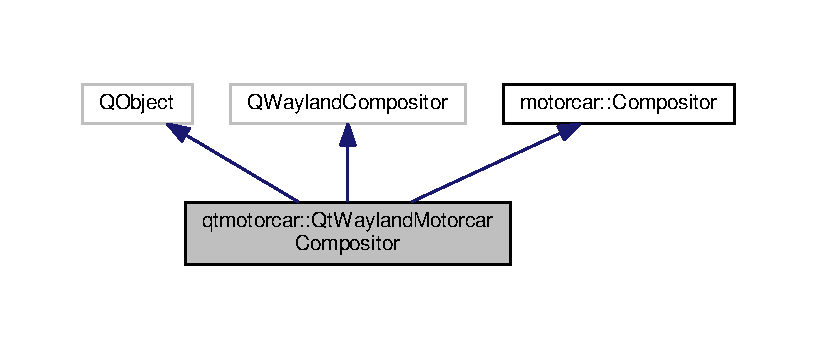
\includegraphics[width=350pt]{classqtmotorcar_1_1QtWaylandMotorcarCompositor__inherit__graph}
\end{center}
\end{figure}


Collaboration diagram for qtmotorcar\-:\-:Qt\-Wayland\-Motorcar\-Compositor\-:
\nopagebreak
\begin{figure}[H]
\begin{center}
\leavevmode
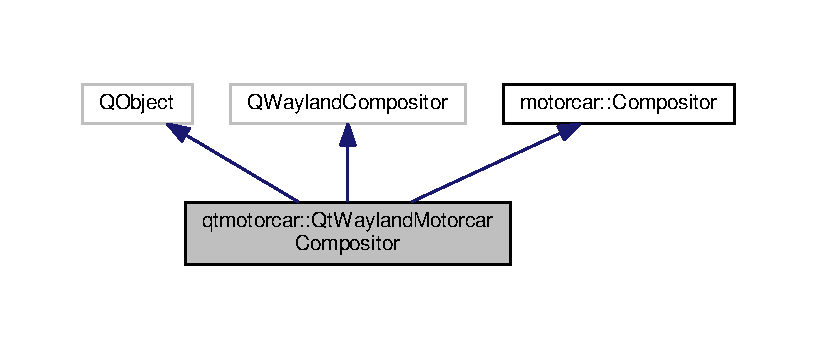
\includegraphics[width=350pt]{classqtmotorcar_1_1QtWaylandMotorcarCompositor__coll__graph}
\end{center}
\end{figure}
\subsection*{Public Member Functions}
\begin{DoxyCompactItemize}
\item 
\hyperlink{classqtmotorcar_1_1QtWaylandMotorcarCompositor_a0de2ac0cbe6d725a501375a84573c470}{Qt\-Wayland\-Motorcar\-Compositor} (\hyperlink{classQOpenGLWindow}{Q\-Open\-G\-L\-Window} $\ast$\hyperlink{structwindow}{window}, Q\-Gui\-Application $\ast$app, \hyperlink{classmotorcar_1_1Scene}{motorcar\-::\-Scene} $\ast$\hyperlink{classqtmotorcar_1_1QtWaylandMotorcarCompositor_a8bb6c8e6a7acad99b814b192534f3ee2}{scene})
\item 
\hyperlink{classqtmotorcar_1_1QtWaylandMotorcarCompositor_a8d0178c57bdbe03ef7e4db6e13900950}{$\sim$\-Qt\-Wayland\-Motorcar\-Compositor} ()
\item 
virtual int \hyperlink{classqtmotorcar_1_1QtWaylandMotorcarCompositor_a34cd3f4acc535584eb066d3fe32ed9bf}{start} () override
\begin{DoxyCompactList}\small\item\em starts the compositor main draw loop \end{DoxyCompactList}\item 
virtual \hyperlink{classmotorcar_1_1OpenGLContext}{motorcar\-::\-Open\-G\-L\-Context} $\ast$ \hyperlink{classqtmotorcar_1_1QtWaylandMotorcarCompositor_a1fb6e9d59011be2912bc9cf51496b191}{get\-Context} () override
\begin{DoxyCompactList}\small\item\em gets the Open\-G\-L context in which the compositing is taking place \end{DoxyCompactList}\item 
struct wl\-\_\-display $\ast$ \hyperlink{classqtmotorcar_1_1QtWaylandMotorcarCompositor_a9e29a67d95d6aa74a08b2a3deed19dfe}{wl\-Display} () override
\item 
\hyperlink{classmotorcar_1_1WaylandSurface}{motorcar\-::\-Wayland\-Surface} $\ast$ \hyperlink{classqtmotorcar_1_1QtWaylandMotorcarCompositor_ad4262e2dce170d25080e5c205fecc5ca}{get\-Surface\-From\-Resource} (struct wl\-\_\-resource $\ast$resource) override
\item 
\hyperlink{classOpenGLData}{Open\-G\-L\-Data} $\ast$ \hyperlink{classqtmotorcar_1_1QtWaylandMotorcarCompositor_a50bc0b510d20d0298b9e164804543f81}{gl\-Data} () const 
\item 
void \hyperlink{classqtmotorcar_1_1QtWaylandMotorcarCompositor_a0122a32ec769e7190b3a2e0a838f0053}{set\-Gl\-Data} (\hyperlink{classOpenGLData}{Open\-G\-L\-Data} $\ast$\hyperlink{classqtmotorcar_1_1QtWaylandMotorcarCompositor_a50bc0b510d20d0298b9e164804543f81}{gl\-Data})
\item 
\hyperlink{classmotorcar_1_1Scene}{motorcar\-::\-Scene} $\ast$ \hyperlink{classqtmotorcar_1_1QtWaylandMotorcarCompositor_a8bb6c8e6a7acad99b814b192534f3ee2}{scene} () const 
\item 
void \hyperlink{classqtmotorcar_1_1QtWaylandMotorcarCompositor_a2a896748e415515de155c22ef70adeb0}{set\-Scene} (\hyperlink{classmotorcar_1_1Scene}{motorcar\-::\-Scene} $\ast$\hyperlink{classqtmotorcar_1_1QtWaylandMotorcarCompositor_a8bb6c8e6a7acad99b814b192534f3ee2}{scene})
\item 
\hyperlink{classqtmotorcar_1_1QtWaylandMotorcarSurface}{Qt\-Wayland\-Motorcar\-Surface} $\ast$ \hyperlink{classqtmotorcar_1_1QtWaylandMotorcarCompositor_a97c4d656c14bd2b6877405d5003fb741}{get\-Motorcar\-Surface} (Q\-Wayland\-Surface $\ast$\hyperlink{simple-egl_8c_a0720952aa1caded45b5bcdce589663a9}{surface}=N\-U\-L\-L) const 
\item 
\hyperlink{classqtmotorcar_1_1QtWaylandMotorcarSeat}{Qt\-Wayland\-Motorcar\-Seat} $\ast$ \hyperlink{classqtmotorcar_1_1QtWaylandMotorcarCompositor_a6104791cebeec6529ec784db17096a38}{default\-Seat} () const 
\item 
void \hyperlink{classqtmotorcar_1_1QtWaylandMotorcarCompositor_a6ea6591a5e3999156f7418f8a61db992}{set\-Default\-Seat} (\hyperlink{classqtmotorcar_1_1QtWaylandMotorcarSeat}{Qt\-Wayland\-Motorcar\-Seat} $\ast$\hyperlink{classqtmotorcar_1_1QtWaylandMotorcarCompositor_a6104791cebeec6529ec784db17096a38}{default\-Seat})
\end{DoxyCompactItemize}
\subsection*{Static Public Member Functions}
\begin{DoxyCompactItemize}
\item 
static \\*
\hyperlink{classqtmotorcar_1_1QtWaylandMotorcarCompositor}{Qt\-Wayland\-Motorcar\-Compositor} $\ast$ \hyperlink{classqtmotorcar_1_1QtWaylandMotorcarCompositor_a169e428e534906108290bb5c4512ca13}{create} (int argc, char $\ast$$\ast$argv, \hyperlink{classmotorcar_1_1Scene}{motorcar\-::\-Scene} $\ast$\hyperlink{classqtmotorcar_1_1QtWaylandMotorcarCompositor_a8bb6c8e6a7acad99b814b192534f3ee2}{scene})
\end{DoxyCompactItemize}
\subsection*{Protected Member Functions}
\begin{DoxyCompactItemize}
\item 
void \hyperlink{classqtmotorcar_1_1QtWaylandMotorcarCompositor_a12ce718691bc19318acd23b981a72cb8}{surface\-Damaged} (Q\-Wayland\-Surface $\ast$\hyperlink{simple-egl_8c_a0720952aa1caded45b5bcdce589663a9}{surface})
\item 
void \hyperlink{classqtmotorcar_1_1QtWaylandMotorcarCompositor_a4bda9a0989cb8c22e7b5d1a687763b61}{surface\-Created} (Q\-Wayland\-Surface $\ast$\hyperlink{simple-egl_8c_a0720952aa1caded45b5bcdce589663a9}{surface})
\item 
Q\-Wayland\-Surface $\ast$ \hyperlink{classqtmotorcar_1_1QtWaylandMotorcarCompositor_adcc9307301b665c9d5ccea73fef01453}{surface\-At} (const Q\-Point\-F \&point, Q\-Point\-F $\ast$local=0)
\item 
bool \hyperlink{classqtmotorcar_1_1QtWaylandMotorcarCompositor_a1d5c76d5c4dfd029d90803d889c07206}{event\-Filter} (Q\-Object $\ast$obj, Q\-Event $\ast$event)
\item 
Q\-Point\-F \hyperlink{classqtmotorcar_1_1QtWaylandMotorcarCompositor_af3c3c2e2dbfd18427c8b38f83f0fa01f}{to\-Surface} (Q\-Wayland\-Surface $\ast$\hyperlink{simple-egl_8c_a0720952aa1caded45b5bcdce589663a9}{surface}, const Q\-Point\-F \&point) const 
\item 
void \hyperlink{classqtmotorcar_1_1QtWaylandMotorcarCompositor_a4555fa6ed0c867668fe735d9192331c7}{set\-Cursor\-Surface} (Q\-Wayland\-Surface $\ast$\hyperlink{simple-egl_8c_a0720952aa1caded45b5bcdce589663a9}{surface}, int hotspot\-X, int hotspot\-Y)
\item 
void \hyperlink{classqtmotorcar_1_1QtWaylandMotorcarCompositor_ac2210c9eaefdc154eac4111807232eb0}{ensure\-Keyboard\-Focus\-Surface} (Q\-Wayland\-Surface $\ast$old\-Surface)
\end{DoxyCompactItemize}


\subsection{Constructor \& Destructor Documentation}
\hypertarget{classqtmotorcar_1_1QtWaylandMotorcarCompositor_a0de2ac0cbe6d725a501375a84573c470}{\index{qtmotorcar\-::\-Qt\-Wayland\-Motorcar\-Compositor@{qtmotorcar\-::\-Qt\-Wayland\-Motorcar\-Compositor}!Qt\-Wayland\-Motorcar\-Compositor@{Qt\-Wayland\-Motorcar\-Compositor}}
\index{Qt\-Wayland\-Motorcar\-Compositor@{Qt\-Wayland\-Motorcar\-Compositor}!qtmotorcar::QtWaylandMotorcarCompositor@{qtmotorcar\-::\-Qt\-Wayland\-Motorcar\-Compositor}}
\subsubsection[{Qt\-Wayland\-Motorcar\-Compositor}]{\setlength{\rightskip}{0pt plus 5cm}Qt\-Wayland\-Motorcar\-Compositor\-::\-Qt\-Wayland\-Motorcar\-Compositor (
\begin{DoxyParamCaption}
\item[{{\bf Q\-Open\-G\-L\-Window} $\ast$}]{window, }
\item[{Q\-Gui\-Application $\ast$}]{app, }
\item[{{\bf motorcar\-::\-Scene} $\ast$}]{scene}
\end{DoxyParamCaption}
)}}\label{classqtmotorcar_1_1QtWaylandMotorcarCompositor_a0de2ac0cbe6d725a501375a84573c470}
\hypertarget{classqtmotorcar_1_1QtWaylandMotorcarCompositor_a8d0178c57bdbe03ef7e4db6e13900950}{\index{qtmotorcar\-::\-Qt\-Wayland\-Motorcar\-Compositor@{qtmotorcar\-::\-Qt\-Wayland\-Motorcar\-Compositor}!$\sim$\-Qt\-Wayland\-Motorcar\-Compositor@{$\sim$\-Qt\-Wayland\-Motorcar\-Compositor}}
\index{$\sim$\-Qt\-Wayland\-Motorcar\-Compositor@{$\sim$\-Qt\-Wayland\-Motorcar\-Compositor}!qtmotorcar::QtWaylandMotorcarCompositor@{qtmotorcar\-::\-Qt\-Wayland\-Motorcar\-Compositor}}
\subsubsection[{$\sim$\-Qt\-Wayland\-Motorcar\-Compositor}]{\setlength{\rightskip}{0pt plus 5cm}Qt\-Wayland\-Motorcar\-Compositor\-::$\sim$\-Qt\-Wayland\-Motorcar\-Compositor (
\begin{DoxyParamCaption}
{}
\end{DoxyParamCaption}
)}}\label{classqtmotorcar_1_1QtWaylandMotorcarCompositor_a8d0178c57bdbe03ef7e4db6e13900950}


\subsection{Member Function Documentation}
\hypertarget{classqtmotorcar_1_1QtWaylandMotorcarCompositor_a169e428e534906108290bb5c4512ca13}{\index{qtmotorcar\-::\-Qt\-Wayland\-Motorcar\-Compositor@{qtmotorcar\-::\-Qt\-Wayland\-Motorcar\-Compositor}!create@{create}}
\index{create@{create}!qtmotorcar::QtWaylandMotorcarCompositor@{qtmotorcar\-::\-Qt\-Wayland\-Motorcar\-Compositor}}
\subsubsection[{create}]{\setlength{\rightskip}{0pt plus 5cm}{\bf Qt\-Wayland\-Motorcar\-Compositor} $\ast$ Qt\-Wayland\-Motorcar\-Compositor\-::create (
\begin{DoxyParamCaption}
\item[{int}]{argc, }
\item[{char $\ast$$\ast$}]{argv, }
\item[{{\bf motorcar\-::\-Scene} $\ast$}]{scene}
\end{DoxyParamCaption}
)\hspace{0.3cm}{\ttfamily [static]}}}\label{classqtmotorcar_1_1QtWaylandMotorcarCompositor_a169e428e534906108290bb5c4512ca13}
\hypertarget{classqtmotorcar_1_1QtWaylandMotorcarCompositor_a6104791cebeec6529ec784db17096a38}{\index{qtmotorcar\-::\-Qt\-Wayland\-Motorcar\-Compositor@{qtmotorcar\-::\-Qt\-Wayland\-Motorcar\-Compositor}!default\-Seat@{default\-Seat}}
\index{default\-Seat@{default\-Seat}!qtmotorcar::QtWaylandMotorcarCompositor@{qtmotorcar\-::\-Qt\-Wayland\-Motorcar\-Compositor}}
\subsubsection[{default\-Seat}]{\setlength{\rightskip}{0pt plus 5cm}{\bf Qt\-Wayland\-Motorcar\-Seat} $\ast$ Qt\-Wayland\-Motorcar\-Compositor\-::default\-Seat (
\begin{DoxyParamCaption}
{}
\end{DoxyParamCaption}
) const}}\label{classqtmotorcar_1_1QtWaylandMotorcarCompositor_a6104791cebeec6529ec784db17096a38}
\hypertarget{classqtmotorcar_1_1QtWaylandMotorcarCompositor_ac2210c9eaefdc154eac4111807232eb0}{\index{qtmotorcar\-::\-Qt\-Wayland\-Motorcar\-Compositor@{qtmotorcar\-::\-Qt\-Wayland\-Motorcar\-Compositor}!ensure\-Keyboard\-Focus\-Surface@{ensure\-Keyboard\-Focus\-Surface}}
\index{ensure\-Keyboard\-Focus\-Surface@{ensure\-Keyboard\-Focus\-Surface}!qtmotorcar::QtWaylandMotorcarCompositor@{qtmotorcar\-::\-Qt\-Wayland\-Motorcar\-Compositor}}
\subsubsection[{ensure\-Keyboard\-Focus\-Surface}]{\setlength{\rightskip}{0pt plus 5cm}void Qt\-Wayland\-Motorcar\-Compositor\-::ensure\-Keyboard\-Focus\-Surface (
\begin{DoxyParamCaption}
\item[{Q\-Wayland\-Surface $\ast$}]{old\-Surface}
\end{DoxyParamCaption}
)\hspace{0.3cm}{\ttfamily [protected]}}}\label{classqtmotorcar_1_1QtWaylandMotorcarCompositor_ac2210c9eaefdc154eac4111807232eb0}
\hypertarget{classqtmotorcar_1_1QtWaylandMotorcarCompositor_a1d5c76d5c4dfd029d90803d889c07206}{\index{qtmotorcar\-::\-Qt\-Wayland\-Motorcar\-Compositor@{qtmotorcar\-::\-Qt\-Wayland\-Motorcar\-Compositor}!event\-Filter@{event\-Filter}}
\index{event\-Filter@{event\-Filter}!qtmotorcar::QtWaylandMotorcarCompositor@{qtmotorcar\-::\-Qt\-Wayland\-Motorcar\-Compositor}}
\subsubsection[{event\-Filter}]{\setlength{\rightskip}{0pt plus 5cm}bool Qt\-Wayland\-Motorcar\-Compositor\-::event\-Filter (
\begin{DoxyParamCaption}
\item[{Q\-Object $\ast$}]{obj, }
\item[{Q\-Event $\ast$}]{event}
\end{DoxyParamCaption}
)\hspace{0.3cm}{\ttfamily [protected]}}}\label{classqtmotorcar_1_1QtWaylandMotorcarCompositor_a1d5c76d5c4dfd029d90803d889c07206}
\hypertarget{classqtmotorcar_1_1QtWaylandMotorcarCompositor_a1fb6e9d59011be2912bc9cf51496b191}{\index{qtmotorcar\-::\-Qt\-Wayland\-Motorcar\-Compositor@{qtmotorcar\-::\-Qt\-Wayland\-Motorcar\-Compositor}!get\-Context@{get\-Context}}
\index{get\-Context@{get\-Context}!qtmotorcar::QtWaylandMotorcarCompositor@{qtmotorcar\-::\-Qt\-Wayland\-Motorcar\-Compositor}}
\subsubsection[{get\-Context}]{\setlength{\rightskip}{0pt plus 5cm}{\bf motorcar\-::\-Open\-G\-L\-Context} $\ast$ Qt\-Wayland\-Motorcar\-Compositor\-::get\-Context (
\begin{DoxyParamCaption}
{}
\end{DoxyParamCaption}
)\hspace{0.3cm}{\ttfamily [override]}, {\ttfamily [virtual]}}}\label{classqtmotorcar_1_1QtWaylandMotorcarCompositor_a1fb6e9d59011be2912bc9cf51496b191}


gets the Open\-G\-L context in which the compositing is taking place 



Implements \hyperlink{classmotorcar_1_1Compositor_afb0a16529f65b5e2ecf8f15524680c57}{motorcar\-::\-Compositor}.

\hypertarget{classqtmotorcar_1_1QtWaylandMotorcarCompositor_a97c4d656c14bd2b6877405d5003fb741}{\index{qtmotorcar\-::\-Qt\-Wayland\-Motorcar\-Compositor@{qtmotorcar\-::\-Qt\-Wayland\-Motorcar\-Compositor}!get\-Motorcar\-Surface@{get\-Motorcar\-Surface}}
\index{get\-Motorcar\-Surface@{get\-Motorcar\-Surface}!qtmotorcar::QtWaylandMotorcarCompositor@{qtmotorcar\-::\-Qt\-Wayland\-Motorcar\-Compositor}}
\subsubsection[{get\-Motorcar\-Surface}]{\setlength{\rightskip}{0pt plus 5cm}{\bf Qt\-Wayland\-Motorcar\-Surface} $\ast$ Qt\-Wayland\-Motorcar\-Compositor\-::get\-Motorcar\-Surface (
\begin{DoxyParamCaption}
\item[{Q\-Wayland\-Surface $\ast$}]{surface = {\ttfamily NULL}}
\end{DoxyParamCaption}
) const}}\label{classqtmotorcar_1_1QtWaylandMotorcarCompositor_a97c4d656c14bd2b6877405d5003fb741}
\hypertarget{classqtmotorcar_1_1QtWaylandMotorcarCompositor_ad4262e2dce170d25080e5c205fecc5ca}{\index{qtmotorcar\-::\-Qt\-Wayland\-Motorcar\-Compositor@{qtmotorcar\-::\-Qt\-Wayland\-Motorcar\-Compositor}!get\-Surface\-From\-Resource@{get\-Surface\-From\-Resource}}
\index{get\-Surface\-From\-Resource@{get\-Surface\-From\-Resource}!qtmotorcar::QtWaylandMotorcarCompositor@{qtmotorcar\-::\-Qt\-Wayland\-Motorcar\-Compositor}}
\subsubsection[{get\-Surface\-From\-Resource}]{\setlength{\rightskip}{0pt plus 5cm}{\bf motorcar\-::\-Wayland\-Surface} $\ast$ Qt\-Wayland\-Motorcar\-Compositor\-::get\-Surface\-From\-Resource (
\begin{DoxyParamCaption}
\item[{struct wl\-\_\-resource $\ast$}]{resource}
\end{DoxyParamCaption}
)\hspace{0.3cm}{\ttfamily [override]}, {\ttfamily [virtual]}}}\label{classqtmotorcar_1_1QtWaylandMotorcarCompositor_ad4262e2dce170d25080e5c205fecc5ca}


Implements \hyperlink{classmotorcar_1_1Compositor_abc7e49b58794334e99a0433389a39929}{motorcar\-::\-Compositor}.

\hypertarget{classqtmotorcar_1_1QtWaylandMotorcarCompositor_a50bc0b510d20d0298b9e164804543f81}{\index{qtmotorcar\-::\-Qt\-Wayland\-Motorcar\-Compositor@{qtmotorcar\-::\-Qt\-Wayland\-Motorcar\-Compositor}!gl\-Data@{gl\-Data}}
\index{gl\-Data@{gl\-Data}!qtmotorcar::QtWaylandMotorcarCompositor@{qtmotorcar\-::\-Qt\-Wayland\-Motorcar\-Compositor}}
\subsubsection[{gl\-Data}]{\setlength{\rightskip}{0pt plus 5cm}{\bf Open\-G\-L\-Data} $\ast$ Qt\-Wayland\-Motorcar\-Compositor\-::gl\-Data (
\begin{DoxyParamCaption}
{}
\end{DoxyParamCaption}
) const}}\label{classqtmotorcar_1_1QtWaylandMotorcarCompositor_a50bc0b510d20d0298b9e164804543f81}
\hypertarget{classqtmotorcar_1_1QtWaylandMotorcarCompositor_a8bb6c8e6a7acad99b814b192534f3ee2}{\index{qtmotorcar\-::\-Qt\-Wayland\-Motorcar\-Compositor@{qtmotorcar\-::\-Qt\-Wayland\-Motorcar\-Compositor}!scene@{scene}}
\index{scene@{scene}!qtmotorcar::QtWaylandMotorcarCompositor@{qtmotorcar\-::\-Qt\-Wayland\-Motorcar\-Compositor}}
\subsubsection[{scene}]{\setlength{\rightskip}{0pt plus 5cm}{\bf motorcar\-::\-Scene} $\ast$ Qt\-Wayland\-Motorcar\-Compositor\-::scene (
\begin{DoxyParamCaption}
{}
\end{DoxyParamCaption}
) const}}\label{classqtmotorcar_1_1QtWaylandMotorcarCompositor_a8bb6c8e6a7acad99b814b192534f3ee2}
\hypertarget{classqtmotorcar_1_1QtWaylandMotorcarCompositor_a4555fa6ed0c867668fe735d9192331c7}{\index{qtmotorcar\-::\-Qt\-Wayland\-Motorcar\-Compositor@{qtmotorcar\-::\-Qt\-Wayland\-Motorcar\-Compositor}!set\-Cursor\-Surface@{set\-Cursor\-Surface}}
\index{set\-Cursor\-Surface@{set\-Cursor\-Surface}!qtmotorcar::QtWaylandMotorcarCompositor@{qtmotorcar\-::\-Qt\-Wayland\-Motorcar\-Compositor}}
\subsubsection[{set\-Cursor\-Surface}]{\setlength{\rightskip}{0pt plus 5cm}void Qt\-Wayland\-Motorcar\-Compositor\-::set\-Cursor\-Surface (
\begin{DoxyParamCaption}
\item[{Q\-Wayland\-Surface $\ast$}]{surface, }
\item[{int}]{hotspot\-X, }
\item[{int}]{hotspot\-Y}
\end{DoxyParamCaption}
)\hspace{0.3cm}{\ttfamily [protected]}}}\label{classqtmotorcar_1_1QtWaylandMotorcarCompositor_a4555fa6ed0c867668fe735d9192331c7}
\hypertarget{classqtmotorcar_1_1QtWaylandMotorcarCompositor_a6ea6591a5e3999156f7418f8a61db992}{\index{qtmotorcar\-::\-Qt\-Wayland\-Motorcar\-Compositor@{qtmotorcar\-::\-Qt\-Wayland\-Motorcar\-Compositor}!set\-Default\-Seat@{set\-Default\-Seat}}
\index{set\-Default\-Seat@{set\-Default\-Seat}!qtmotorcar::QtWaylandMotorcarCompositor@{qtmotorcar\-::\-Qt\-Wayland\-Motorcar\-Compositor}}
\subsubsection[{set\-Default\-Seat}]{\setlength{\rightskip}{0pt plus 5cm}void Qt\-Wayland\-Motorcar\-Compositor\-::set\-Default\-Seat (
\begin{DoxyParamCaption}
\item[{{\bf Qt\-Wayland\-Motorcar\-Seat} $\ast$}]{default\-Seat}
\end{DoxyParamCaption}
)}}\label{classqtmotorcar_1_1QtWaylandMotorcarCompositor_a6ea6591a5e3999156f7418f8a61db992}
\hypertarget{classqtmotorcar_1_1QtWaylandMotorcarCompositor_a0122a32ec769e7190b3a2e0a838f0053}{\index{qtmotorcar\-::\-Qt\-Wayland\-Motorcar\-Compositor@{qtmotorcar\-::\-Qt\-Wayland\-Motorcar\-Compositor}!set\-Gl\-Data@{set\-Gl\-Data}}
\index{set\-Gl\-Data@{set\-Gl\-Data}!qtmotorcar::QtWaylandMotorcarCompositor@{qtmotorcar\-::\-Qt\-Wayland\-Motorcar\-Compositor}}
\subsubsection[{set\-Gl\-Data}]{\setlength{\rightskip}{0pt plus 5cm}void Qt\-Wayland\-Motorcar\-Compositor\-::set\-Gl\-Data (
\begin{DoxyParamCaption}
\item[{{\bf Open\-G\-L\-Data} $\ast$}]{gl\-Data}
\end{DoxyParamCaption}
)}}\label{classqtmotorcar_1_1QtWaylandMotorcarCompositor_a0122a32ec769e7190b3a2e0a838f0053}
\hypertarget{classqtmotorcar_1_1QtWaylandMotorcarCompositor_a2a896748e415515de155c22ef70adeb0}{\index{qtmotorcar\-::\-Qt\-Wayland\-Motorcar\-Compositor@{qtmotorcar\-::\-Qt\-Wayland\-Motorcar\-Compositor}!set\-Scene@{set\-Scene}}
\index{set\-Scene@{set\-Scene}!qtmotorcar::QtWaylandMotorcarCompositor@{qtmotorcar\-::\-Qt\-Wayland\-Motorcar\-Compositor}}
\subsubsection[{set\-Scene}]{\setlength{\rightskip}{0pt plus 5cm}void Qt\-Wayland\-Motorcar\-Compositor\-::set\-Scene (
\begin{DoxyParamCaption}
\item[{{\bf motorcar\-::\-Scene} $\ast$}]{scene}
\end{DoxyParamCaption}
)}}\label{classqtmotorcar_1_1QtWaylandMotorcarCompositor_a2a896748e415515de155c22ef70adeb0}
\hypertarget{classqtmotorcar_1_1QtWaylandMotorcarCompositor_a34cd3f4acc535584eb066d3fe32ed9bf}{\index{qtmotorcar\-::\-Qt\-Wayland\-Motorcar\-Compositor@{qtmotorcar\-::\-Qt\-Wayland\-Motorcar\-Compositor}!start@{start}}
\index{start@{start}!qtmotorcar::QtWaylandMotorcarCompositor@{qtmotorcar\-::\-Qt\-Wayland\-Motorcar\-Compositor}}
\subsubsection[{start}]{\setlength{\rightskip}{0pt plus 5cm}int Qt\-Wayland\-Motorcar\-Compositor\-::start (
\begin{DoxyParamCaption}
{}
\end{DoxyParamCaption}
)\hspace{0.3cm}{\ttfamily [override]}, {\ttfamily [virtual]}}}\label{classqtmotorcar_1_1QtWaylandMotorcarCompositor_a34cd3f4acc535584eb066d3fe32ed9bf}


starts the compositor main draw loop 



Implements \hyperlink{classmotorcar_1_1Compositor_a9d4b703e99386360996087a1100fae52}{motorcar\-::\-Compositor}.

\hypertarget{classqtmotorcar_1_1QtWaylandMotorcarCompositor_adcc9307301b665c9d5ccea73fef01453}{\index{qtmotorcar\-::\-Qt\-Wayland\-Motorcar\-Compositor@{qtmotorcar\-::\-Qt\-Wayland\-Motorcar\-Compositor}!surface\-At@{surface\-At}}
\index{surface\-At@{surface\-At}!qtmotorcar::QtWaylandMotorcarCompositor@{qtmotorcar\-::\-Qt\-Wayland\-Motorcar\-Compositor}}
\subsubsection[{surface\-At}]{\setlength{\rightskip}{0pt plus 5cm}Q\-Wayland\-Surface $\ast$ Qt\-Wayland\-Motorcar\-Compositor\-::surface\-At (
\begin{DoxyParamCaption}
\item[{const Q\-Point\-F \&}]{point, }
\item[{Q\-Point\-F $\ast$}]{local = {\ttfamily 0}}
\end{DoxyParamCaption}
)\hspace{0.3cm}{\ttfamily [protected]}}}\label{classqtmotorcar_1_1QtWaylandMotorcarCompositor_adcc9307301b665c9d5ccea73fef01453}
\hypertarget{classqtmotorcar_1_1QtWaylandMotorcarCompositor_a4bda9a0989cb8c22e7b5d1a687763b61}{\index{qtmotorcar\-::\-Qt\-Wayland\-Motorcar\-Compositor@{qtmotorcar\-::\-Qt\-Wayland\-Motorcar\-Compositor}!surface\-Created@{surface\-Created}}
\index{surface\-Created@{surface\-Created}!qtmotorcar::QtWaylandMotorcarCompositor@{qtmotorcar\-::\-Qt\-Wayland\-Motorcar\-Compositor}}
\subsubsection[{surface\-Created}]{\setlength{\rightskip}{0pt plus 5cm}void Qt\-Wayland\-Motorcar\-Compositor\-::surface\-Created (
\begin{DoxyParamCaption}
\item[{Q\-Wayland\-Surface $\ast$}]{surface}
\end{DoxyParamCaption}
)\hspace{0.3cm}{\ttfamily [protected]}}}\label{classqtmotorcar_1_1QtWaylandMotorcarCompositor_a4bda9a0989cb8c22e7b5d1a687763b61}
\hypertarget{classqtmotorcar_1_1QtWaylandMotorcarCompositor_a12ce718691bc19318acd23b981a72cb8}{\index{qtmotorcar\-::\-Qt\-Wayland\-Motorcar\-Compositor@{qtmotorcar\-::\-Qt\-Wayland\-Motorcar\-Compositor}!surface\-Damaged@{surface\-Damaged}}
\index{surface\-Damaged@{surface\-Damaged}!qtmotorcar::QtWaylandMotorcarCompositor@{qtmotorcar\-::\-Qt\-Wayland\-Motorcar\-Compositor}}
\subsubsection[{surface\-Damaged}]{\setlength{\rightskip}{0pt plus 5cm}void Qt\-Wayland\-Motorcar\-Compositor\-::surface\-Damaged (
\begin{DoxyParamCaption}
\item[{Q\-Wayland\-Surface $\ast$}]{surface}
\end{DoxyParamCaption}
)\hspace{0.3cm}{\ttfamily [protected]}}}\label{classqtmotorcar_1_1QtWaylandMotorcarCompositor_a12ce718691bc19318acd23b981a72cb8}
\hypertarget{classqtmotorcar_1_1QtWaylandMotorcarCompositor_af3c3c2e2dbfd18427c8b38f83f0fa01f}{\index{qtmotorcar\-::\-Qt\-Wayland\-Motorcar\-Compositor@{qtmotorcar\-::\-Qt\-Wayland\-Motorcar\-Compositor}!to\-Surface@{to\-Surface}}
\index{to\-Surface@{to\-Surface}!qtmotorcar::QtWaylandMotorcarCompositor@{qtmotorcar\-::\-Qt\-Wayland\-Motorcar\-Compositor}}
\subsubsection[{to\-Surface}]{\setlength{\rightskip}{0pt plus 5cm}Q\-Point\-F Qt\-Wayland\-Motorcar\-Compositor\-::to\-Surface (
\begin{DoxyParamCaption}
\item[{Q\-Wayland\-Surface $\ast$}]{surface, }
\item[{const Q\-Point\-F \&}]{point}
\end{DoxyParamCaption}
) const\hspace{0.3cm}{\ttfamily [protected]}}}\label{classqtmotorcar_1_1QtWaylandMotorcarCompositor_af3c3c2e2dbfd18427c8b38f83f0fa01f}
\hypertarget{classqtmotorcar_1_1QtWaylandMotorcarCompositor_a9e29a67d95d6aa74a08b2a3deed19dfe}{\index{qtmotorcar\-::\-Qt\-Wayland\-Motorcar\-Compositor@{qtmotorcar\-::\-Qt\-Wayland\-Motorcar\-Compositor}!wl\-Display@{wl\-Display}}
\index{wl\-Display@{wl\-Display}!qtmotorcar::QtWaylandMotorcarCompositor@{qtmotorcar\-::\-Qt\-Wayland\-Motorcar\-Compositor}}
\subsubsection[{wl\-Display}]{\setlength{\rightskip}{0pt plus 5cm}wl\-\_\-display $\ast$ Qt\-Wayland\-Motorcar\-Compositor\-::wl\-Display (
\begin{DoxyParamCaption}
{}
\end{DoxyParamCaption}
)\hspace{0.3cm}{\ttfamily [override]}, {\ttfamily [virtual]}}}\label{classqtmotorcar_1_1QtWaylandMotorcarCompositor_a9e29a67d95d6aa74a08b2a3deed19dfe}


Implements \hyperlink{classmotorcar_1_1Compositor_a19115510ba397b13d439eac5323ea998}{motorcar\-::\-Compositor}.



The documentation for this class was generated from the following files\-:\begin{DoxyCompactItemize}
\item 
/media/dave/e89b5eb4-\/4b10-\/4edf-\/8ad5-\/0d046a46b978/dave/thesis/qtwayland-\/motorcar-\/compositor/qt/src/\hyperlink{qtwaylandmotorcarcompositor_8h}{qtwaylandmotorcarcompositor.\-h}\item 
/media/dave/e89b5eb4-\/4b10-\/4edf-\/8ad5-\/0d046a46b978/dave/thesis/qtwayland-\/motorcar-\/compositor/qt/src/\hyperlink{qtwaylandmotorcarcompositor_8cpp}{qtwaylandmotorcarcompositor.\-cpp}\end{DoxyCompactItemize}

\hypertarget{classqtmotorcar_1_1QtWaylandMotorcarOpenGLContext}{\section{qtmotorcar\-:\-:Qt\-Wayland\-Motorcar\-Open\-G\-L\-Context Class Reference}
\label{classqtmotorcar_1_1QtWaylandMotorcarOpenGLContext}\index{qtmotorcar\-::\-Qt\-Wayland\-Motorcar\-Open\-G\-L\-Context@{qtmotorcar\-::\-Qt\-Wayland\-Motorcar\-Open\-G\-L\-Context}}
}


{\ttfamily \#include $<$qtwaylandmotorcaropenglcontext.\-h$>$}



Inheritance diagram for qtmotorcar\-:\-:Qt\-Wayland\-Motorcar\-Open\-G\-L\-Context\-:
\nopagebreak
\begin{figure}[H]
\begin{center}
\leavevmode
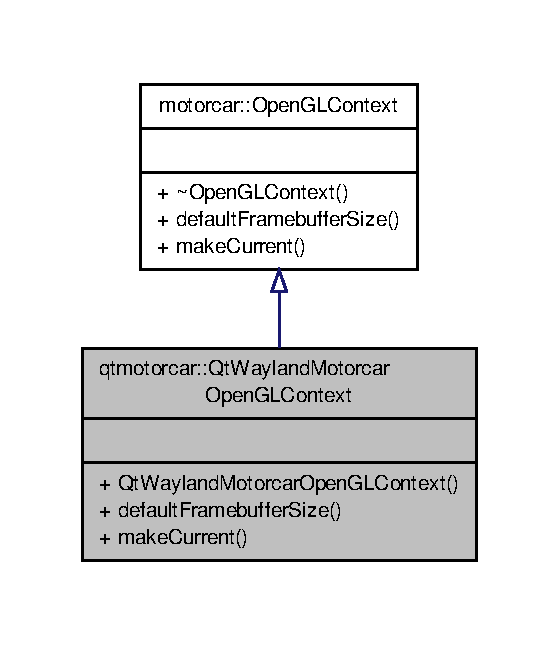
\includegraphics[width=268pt]{classqtmotorcar_1_1QtWaylandMotorcarOpenGLContext__inherit__graph}
\end{center}
\end{figure}


Collaboration diagram for qtmotorcar\-:\-:Qt\-Wayland\-Motorcar\-Open\-G\-L\-Context\-:
\nopagebreak
\begin{figure}[H]
\begin{center}
\leavevmode
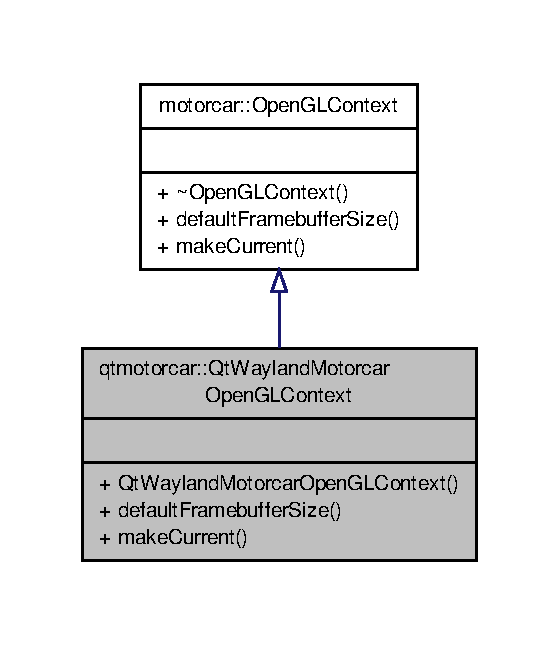
\includegraphics[width=268pt]{classqtmotorcar_1_1QtWaylandMotorcarOpenGLContext__coll__graph}
\end{center}
\end{figure}
\subsection*{Public Member Functions}
\begin{DoxyCompactItemize}
\item 
\hyperlink{classqtmotorcar_1_1QtWaylandMotorcarOpenGLContext_a18441ac9b0796170b33fdfb8c1154e30}{Qt\-Wayland\-Motorcar\-Open\-G\-L\-Context} (\hyperlink{classQOpenGLWindow}{Q\-Open\-G\-L\-Window} $\ast$window)
\item 
glm\-::ivec2 \hyperlink{classqtmotorcar_1_1QtWaylandMotorcarOpenGLContext_ab2a51af3b29de69f0a2d3d60d3bdbe82}{default\-Framebuffer\-Size} () override
\item 
void \hyperlink{classqtmotorcar_1_1QtWaylandMotorcarOpenGLContext_ae5f00ad8258f7c03466ad114b64e250a}{make\-Current} () override
\end{DoxyCompactItemize}


\subsection{Constructor \& Destructor Documentation}
\hypertarget{classqtmotorcar_1_1QtWaylandMotorcarOpenGLContext_a18441ac9b0796170b33fdfb8c1154e30}{\index{qtmotorcar\-::\-Qt\-Wayland\-Motorcar\-Open\-G\-L\-Context@{qtmotorcar\-::\-Qt\-Wayland\-Motorcar\-Open\-G\-L\-Context}!Qt\-Wayland\-Motorcar\-Open\-G\-L\-Context@{Qt\-Wayland\-Motorcar\-Open\-G\-L\-Context}}
\index{Qt\-Wayland\-Motorcar\-Open\-G\-L\-Context@{Qt\-Wayland\-Motorcar\-Open\-G\-L\-Context}!qtmotorcar::QtWaylandMotorcarOpenGLContext@{qtmotorcar\-::\-Qt\-Wayland\-Motorcar\-Open\-G\-L\-Context}}
\subsubsection[{Qt\-Wayland\-Motorcar\-Open\-G\-L\-Context}]{\setlength{\rightskip}{0pt plus 5cm}qtmotorcar\-::\-Qt\-Wayland\-Motorcar\-Open\-G\-L\-Context\-::\-Qt\-Wayland\-Motorcar\-Open\-G\-L\-Context (
\begin{DoxyParamCaption}
\item[{{\bf Q\-Open\-G\-L\-Window} $\ast$}]{window}
\end{DoxyParamCaption}
)}}\label{classqtmotorcar_1_1QtWaylandMotorcarOpenGLContext_a18441ac9b0796170b33fdfb8c1154e30}


\subsection{Member Function Documentation}
\hypertarget{classqtmotorcar_1_1QtWaylandMotorcarOpenGLContext_ab2a51af3b29de69f0a2d3d60d3bdbe82}{\index{qtmotorcar\-::\-Qt\-Wayland\-Motorcar\-Open\-G\-L\-Context@{qtmotorcar\-::\-Qt\-Wayland\-Motorcar\-Open\-G\-L\-Context}!default\-Framebuffer\-Size@{default\-Framebuffer\-Size}}
\index{default\-Framebuffer\-Size@{default\-Framebuffer\-Size}!qtmotorcar::QtWaylandMotorcarOpenGLContext@{qtmotorcar\-::\-Qt\-Wayland\-Motorcar\-Open\-G\-L\-Context}}
\subsubsection[{default\-Framebuffer\-Size}]{\setlength{\rightskip}{0pt plus 5cm}glm\-::ivec2 qtmotorcar\-::\-Qt\-Wayland\-Motorcar\-Open\-G\-L\-Context\-::default\-Framebuffer\-Size (
\begin{DoxyParamCaption}
{}
\end{DoxyParamCaption}
)\hspace{0.3cm}{\ttfamily [override]}, {\ttfamily [virtual]}}}\label{classqtmotorcar_1_1QtWaylandMotorcarOpenGLContext_ab2a51af3b29de69f0a2d3d60d3bdbe82}


Implements \hyperlink{classmotorcar_1_1OpenGLContext_a4a60274f217b9d71ff54ad60351b4127}{motorcar\-::\-Open\-G\-L\-Context}.

\hypertarget{classqtmotorcar_1_1QtWaylandMotorcarOpenGLContext_ae5f00ad8258f7c03466ad114b64e250a}{\index{qtmotorcar\-::\-Qt\-Wayland\-Motorcar\-Open\-G\-L\-Context@{qtmotorcar\-::\-Qt\-Wayland\-Motorcar\-Open\-G\-L\-Context}!make\-Current@{make\-Current}}
\index{make\-Current@{make\-Current}!qtmotorcar::QtWaylandMotorcarOpenGLContext@{qtmotorcar\-::\-Qt\-Wayland\-Motorcar\-Open\-G\-L\-Context}}
\subsubsection[{make\-Current}]{\setlength{\rightskip}{0pt plus 5cm}void qtmotorcar\-::\-Qt\-Wayland\-Motorcar\-Open\-G\-L\-Context\-::make\-Current (
\begin{DoxyParamCaption}
{}
\end{DoxyParamCaption}
)\hspace{0.3cm}{\ttfamily [override]}, {\ttfamily [virtual]}}}\label{classqtmotorcar_1_1QtWaylandMotorcarOpenGLContext_ae5f00ad8258f7c03466ad114b64e250a}


Implements \hyperlink{classmotorcar_1_1OpenGLContext_ae8b9c712092d01b69766469ab196ab80}{motorcar\-::\-Open\-G\-L\-Context}.



The documentation for this class was generated from the following files\-:\begin{DoxyCompactItemize}
\item 
/home/dave/thesis/qtwayland-\/motorcar-\/compositor/qt/src/\hyperlink{qtwaylandmotorcaropenglcontext_8h}{qtwaylandmotorcaropenglcontext.\-h}\item 
/home/dave/thesis/qtwayland-\/motorcar-\/compositor/qt/src/\hyperlink{qtwaylandmotorcaropenglcontext_8cpp}{qtwaylandmotorcaropenglcontext.\-cpp}\end{DoxyCompactItemize}

\hypertarget{classqtmotorcar_1_1QtWaylandMotorcarSeat}{\section{qtmotorcar\-:\-:Qt\-Wayland\-Motorcar\-Seat Class Reference}
\label{classqtmotorcar_1_1QtWaylandMotorcarSeat}\index{qtmotorcar\-::\-Qt\-Wayland\-Motorcar\-Seat@{qtmotorcar\-::\-Qt\-Wayland\-Motorcar\-Seat}}
}


{\ttfamily \#include $<$qtwaylandmotorcarseat.\-h$>$}



Inheritance diagram for qtmotorcar\-:\-:Qt\-Wayland\-Motorcar\-Seat\-:
\nopagebreak
\begin{figure}[H]
\begin{center}
\leavevmode
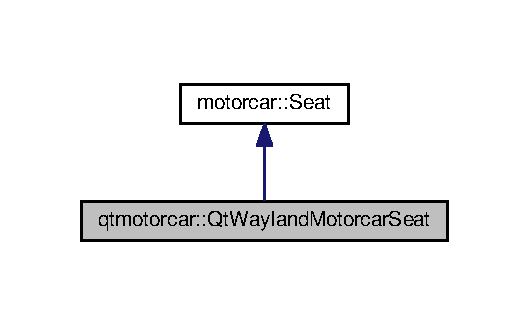
\includegraphics[width=254pt]{classqtmotorcar_1_1QtWaylandMotorcarSeat__inherit__graph}
\end{center}
\end{figure}


Collaboration diagram for qtmotorcar\-:\-:Qt\-Wayland\-Motorcar\-Seat\-:
\nopagebreak
\begin{figure}[H]
\begin{center}
\leavevmode
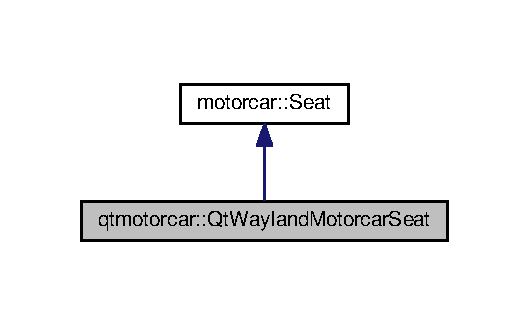
\includegraphics[width=254pt]{classqtmotorcar_1_1QtWaylandMotorcarSeat__coll__graph}
\end{center}
\end{figure}
\subsection*{Public Member Functions}
\begin{DoxyCompactItemize}
\item 
\hyperlink{classqtmotorcar_1_1QtWaylandMotorcarSeat_aa4c5118600488b117ebc9068a84260a9}{Qt\-Wayland\-Motorcar\-Seat} (Q\-Wayland\-Input\-Device $\ast$\hyperlink{classqtmotorcar_1_1QtWaylandMotorcarSeat_a42ef94778942f39aa38deab1bf1beca2}{input\-Device})
\item 
Q\-Wayland\-Input\-Device $\ast$ \hyperlink{classqtmotorcar_1_1QtWaylandMotorcarSeat_a42ef94778942f39aa38deab1bf1beca2}{input\-Device} () const 
\item 
void \hyperlink{classqtmotorcar_1_1QtWaylandMotorcarSeat_a91893bbc681da2b5c8e6a5429b460aff}{set\-Input\-Device} (Q\-Wayland\-Input\-Device $\ast$\hyperlink{classqtmotorcar_1_1QtWaylandMotorcarSeat_a42ef94778942f39aa38deab1bf1beca2}{input\-Device})
\item 
void \hyperlink{classqtmotorcar_1_1QtWaylandMotorcarSeat_a28e6eb540028abe6d70ecd5b7320d6aa}{set\-Keyboard\-Focus} (\hyperlink{classmotorcar_1_1WaylandSurface}{motorcar\-::\-Wayland\-Surface} $\ast$\hyperlink{classmotorcar_1_1Seat_a4ac963bf0d54b6e4a77c0594b37d756f}{keyboard\-Focus}) override
\item 
void \hyperlink{classqtmotorcar_1_1QtWaylandMotorcarSeat_a60932e1f7bd1e626b3427c6b63b80484}{set\-Pointer\-Focus} (\hyperlink{classmotorcar_1_1WaylandSurface}{motorcar\-::\-Wayland\-Surface} $\ast$\hyperlink{classmotorcar_1_1Seat_a996631e534a7c9424245c03c1781fd2a}{pointer\-Focus}, glm\-::vec2 local\-Position) override
\end{DoxyCompactItemize}


\subsection{Constructor \& Destructor Documentation}
\hypertarget{classqtmotorcar_1_1QtWaylandMotorcarSeat_aa4c5118600488b117ebc9068a84260a9}{\index{qtmotorcar\-::\-Qt\-Wayland\-Motorcar\-Seat@{qtmotorcar\-::\-Qt\-Wayland\-Motorcar\-Seat}!Qt\-Wayland\-Motorcar\-Seat@{Qt\-Wayland\-Motorcar\-Seat}}
\index{Qt\-Wayland\-Motorcar\-Seat@{Qt\-Wayland\-Motorcar\-Seat}!qtmotorcar::QtWaylandMotorcarSeat@{qtmotorcar\-::\-Qt\-Wayland\-Motorcar\-Seat}}
\subsubsection[{Qt\-Wayland\-Motorcar\-Seat}]{\setlength{\rightskip}{0pt plus 5cm}Qt\-Wayland\-Motorcar\-Seat\-::\-Qt\-Wayland\-Motorcar\-Seat (
\begin{DoxyParamCaption}
\item[{Q\-Wayland\-Input\-Device $\ast$}]{input\-Device}
\end{DoxyParamCaption}
)}}\label{classqtmotorcar_1_1QtWaylandMotorcarSeat_aa4c5118600488b117ebc9068a84260a9}


\subsection{Member Function Documentation}
\hypertarget{classqtmotorcar_1_1QtWaylandMotorcarSeat_a42ef94778942f39aa38deab1bf1beca2}{\index{qtmotorcar\-::\-Qt\-Wayland\-Motorcar\-Seat@{qtmotorcar\-::\-Qt\-Wayland\-Motorcar\-Seat}!input\-Device@{input\-Device}}
\index{input\-Device@{input\-Device}!qtmotorcar::QtWaylandMotorcarSeat@{qtmotorcar\-::\-Qt\-Wayland\-Motorcar\-Seat}}
\subsubsection[{input\-Device}]{\setlength{\rightskip}{0pt plus 5cm}Q\-Wayland\-Input\-Device $\ast$ Qt\-Wayland\-Motorcar\-Seat\-::input\-Device (
\begin{DoxyParamCaption}
{}
\end{DoxyParamCaption}
) const}}\label{classqtmotorcar_1_1QtWaylandMotorcarSeat_a42ef94778942f39aa38deab1bf1beca2}
\hypertarget{classqtmotorcar_1_1QtWaylandMotorcarSeat_a91893bbc681da2b5c8e6a5429b460aff}{\index{qtmotorcar\-::\-Qt\-Wayland\-Motorcar\-Seat@{qtmotorcar\-::\-Qt\-Wayland\-Motorcar\-Seat}!set\-Input\-Device@{set\-Input\-Device}}
\index{set\-Input\-Device@{set\-Input\-Device}!qtmotorcar::QtWaylandMotorcarSeat@{qtmotorcar\-::\-Qt\-Wayland\-Motorcar\-Seat}}
\subsubsection[{set\-Input\-Device}]{\setlength{\rightskip}{0pt plus 5cm}void Qt\-Wayland\-Motorcar\-Seat\-::set\-Input\-Device (
\begin{DoxyParamCaption}
\item[{Q\-Wayland\-Input\-Device $\ast$}]{input\-Device}
\end{DoxyParamCaption}
)}}\label{classqtmotorcar_1_1QtWaylandMotorcarSeat_a91893bbc681da2b5c8e6a5429b460aff}
\hypertarget{classqtmotorcar_1_1QtWaylandMotorcarSeat_a28e6eb540028abe6d70ecd5b7320d6aa}{\index{qtmotorcar\-::\-Qt\-Wayland\-Motorcar\-Seat@{qtmotorcar\-::\-Qt\-Wayland\-Motorcar\-Seat}!set\-Keyboard\-Focus@{set\-Keyboard\-Focus}}
\index{set\-Keyboard\-Focus@{set\-Keyboard\-Focus}!qtmotorcar::QtWaylandMotorcarSeat@{qtmotorcar\-::\-Qt\-Wayland\-Motorcar\-Seat}}
\subsubsection[{set\-Keyboard\-Focus}]{\setlength{\rightskip}{0pt plus 5cm}void Qt\-Wayland\-Motorcar\-Seat\-::set\-Keyboard\-Focus (
\begin{DoxyParamCaption}
\item[{{\bf motorcar\-::\-Wayland\-Surface} $\ast$}]{keyboard\-Focus}
\end{DoxyParamCaption}
)\hspace{0.3cm}{\ttfamily [override]}, {\ttfamily [virtual]}}}\label{classqtmotorcar_1_1QtWaylandMotorcarSeat_a28e6eb540028abe6d70ecd5b7320d6aa}


Reimplemented from \hyperlink{classmotorcar_1_1Seat_ab8f8eb12135b5db96238c37653fb54d1}{motorcar\-::\-Seat}.

\hypertarget{classqtmotorcar_1_1QtWaylandMotorcarSeat_a60932e1f7bd1e626b3427c6b63b80484}{\index{qtmotorcar\-::\-Qt\-Wayland\-Motorcar\-Seat@{qtmotorcar\-::\-Qt\-Wayland\-Motorcar\-Seat}!set\-Pointer\-Focus@{set\-Pointer\-Focus}}
\index{set\-Pointer\-Focus@{set\-Pointer\-Focus}!qtmotorcar::QtWaylandMotorcarSeat@{qtmotorcar\-::\-Qt\-Wayland\-Motorcar\-Seat}}
\subsubsection[{set\-Pointer\-Focus}]{\setlength{\rightskip}{0pt plus 5cm}void Qt\-Wayland\-Motorcar\-Seat\-::set\-Pointer\-Focus (
\begin{DoxyParamCaption}
\item[{{\bf motorcar\-::\-Wayland\-Surface} $\ast$}]{pointer\-Focus, }
\item[{glm\-::vec2}]{local\-Position}
\end{DoxyParamCaption}
)\hspace{0.3cm}{\ttfamily [override]}, {\ttfamily [virtual]}}}\label{classqtmotorcar_1_1QtWaylandMotorcarSeat_a60932e1f7bd1e626b3427c6b63b80484}


Reimplemented from \hyperlink{classmotorcar_1_1Seat_a0f7254a717c97aba66b15ca8d437734c}{motorcar\-::\-Seat}.



The documentation for this class was generated from the following files\-:\begin{DoxyCompactItemize}
\item 
/home/dave/thesis/motorcar/src/compositor/qt/\hyperlink{qtwaylandmotorcarseat_8h}{qtwaylandmotorcarseat.\-h}\item 
/home/dave/thesis/motorcar/src/compositor/qt/\hyperlink{qtwaylandmotorcarseat_8cpp}{qtwaylandmotorcarseat.\-cpp}\end{DoxyCompactItemize}

\hypertarget{classqtmotorcar_1_1QtWaylandMotorcarSurface}{\section{qtmotorcar\-:\-:Qt\-Wayland\-Motorcar\-Surface Class Reference}
\label{classqtmotorcar_1_1QtWaylandMotorcarSurface}\index{qtmotorcar\-::\-Qt\-Wayland\-Motorcar\-Surface@{qtmotorcar\-::\-Qt\-Wayland\-Motorcar\-Surface}}
}


{\ttfamily \#include $<$qtwaylandmotorcarsurface.\-h$>$}



Inheritance diagram for qtmotorcar\-:\-:Qt\-Wayland\-Motorcar\-Surface\-:
\nopagebreak
\begin{figure}[H]
\begin{center}
\leavevmode
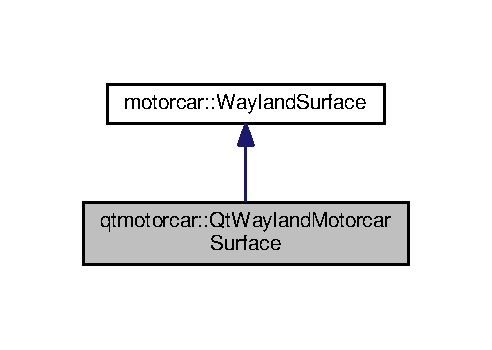
\includegraphics[width=236pt]{classqtmotorcar_1_1QtWaylandMotorcarSurface__inherit__graph}
\end{center}
\end{figure}


Collaboration diagram for qtmotorcar\-:\-:Qt\-Wayland\-Motorcar\-Surface\-:
\nopagebreak
\begin{figure}[H]
\begin{center}
\leavevmode
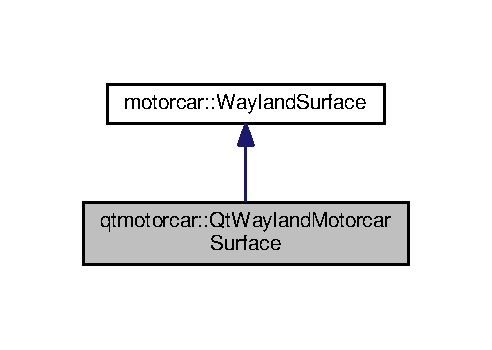
\includegraphics[width=236pt]{classqtmotorcar_1_1QtWaylandMotorcarSurface__coll__graph}
\end{center}
\end{figure}
\subsection*{Public Member Functions}
\begin{DoxyCompactItemize}
\item 
\hyperlink{classqtmotorcar_1_1QtWaylandMotorcarSurface_a054d4981e7da338c72e4fa6572869b60}{Qt\-Wayland\-Motorcar\-Surface} (Q\-Wayland\-Surface $\ast$\hyperlink{simple-egl_8cpp_a0720952aa1caded45b5bcdce589663a9}{surface}, \hyperlink{classqtmotorcar_1_1QtWaylandMotorcarCompositor}{Qt\-Wayland\-Motorcar\-Compositor} $\ast$compositor, \hyperlink{classmotorcar_1_1WaylandSurface_a7715a41b6776800656722407ec01e0a5}{motorcar\-::\-Wayland\-Surface\-::\-Surface\-Type} \hyperlink{classmotorcar_1_1WaylandSurface_a0e6e5e2455666f607a8ddb2479ba8e88}{type})
\item 
\hyperlink{classqtmotorcar_1_1QtWaylandMotorcarSurface_a0d9d57d75c14c209484174e47308f72f}{$\sim$\-Qt\-Wayland\-Motorcar\-Surface} ()
\item 
G\-Luint \hyperlink{classqtmotorcar_1_1QtWaylandMotorcarSurface_a573c52cdacb8f16c06ecd111bddabef6}{texture} () override
\begin{DoxyCompactList}\small\item\em Get the texture handle for this surface. \end{DoxyCompactList}\item 
glm\-::ivec2 \hyperlink{classqtmotorcar_1_1QtWaylandMotorcarSurface_ad5e6f75c146a2952652deaf866ee22a7}{size} () override
\begin{DoxyCompactList}\small\item\em Get the size of this surface in surface local coordinates. \end{DoxyCompactList}\item 
void \hyperlink{classqtmotorcar_1_1QtWaylandMotorcarSurface_abb0d9d5b6a226ab201fc1c0065d1843a}{set\-Size} (glm\-::ivec2 new\-Size) override
\begin{DoxyCompactList}\small\item\em Set the size of this surface in surface local coordinates. \end{DoxyCompactList}\item 
glm\-::ivec2 \hyperlink{classqtmotorcar_1_1QtWaylandMotorcarSurface_ad405b91565405e6a08d86ac5d59f3f08}{position} () override
\begin{DoxyCompactList}\small\item\em Get the position of this surface in parent surface-\/local coordinates. \end{DoxyCompactList}\item 
\hyperlink{classmotorcar_1_1WaylandSurface_a12a62c259b5041c6780c703ec2f12f01}{Wayland\-Surface} $\ast$ \hyperlink{classqtmotorcar_1_1QtWaylandMotorcarSurface_a3b0aed06d7ed9287497bc342f9fc787b}{parent\-Surface} () override
\begin{DoxyCompactList}\small\item\em return the parent surface \end{DoxyCompactList}\item 
void \hyperlink{classqtmotorcar_1_1QtWaylandMotorcarSurface_ae898706dcf80a2f00ed2477c570dcebe}{prepare} () override
\begin{DoxyCompactList}\small\item\em do any per-\/frame setup required for drawing \end{DoxyCompactList}\item 
void \hyperlink{classqtmotorcar_1_1QtWaylandMotorcarSurface_a7deebcf58954f82c8d5741af054414a7}{send\-Event} (const \hyperlink{classmotorcar_1_1Event}{motorcar\-::\-Event} \&event) override
\item 
bool \hyperlink{classqtmotorcar_1_1QtWaylandMotorcarSurface_a3bea85a2a6a3079e60c3b37dd08aebc6}{valid} () override
\begin{DoxyCompactList}\small\item\em returns whether or not the surface is ready to draw \end{DoxyCompactList}\item 
Q\-Wayland\-Surface $\ast$ \hyperlink{classqtmotorcar_1_1QtWaylandMotorcarSurface_aeac2b36246941755d0bedaf1c9fe773b}{surface} () const 
\item 
void \hyperlink{classqtmotorcar_1_1QtWaylandMotorcarSurface_aa7921de176d4d39fe076f145dd382e75}{set\-Surface} (Q\-Wayland\-Surface $\ast$\hyperlink{simple-egl_8cpp_a0720952aa1caded45b5bcdce589663a9}{surface})
\end{DoxyCompactItemize}
\subsection*{Additional Inherited Members}


\subsection{Constructor \& Destructor Documentation}
\hypertarget{classqtmotorcar_1_1QtWaylandMotorcarSurface_a054d4981e7da338c72e4fa6572869b60}{\index{qtmotorcar\-::\-Qt\-Wayland\-Motorcar\-Surface@{qtmotorcar\-::\-Qt\-Wayland\-Motorcar\-Surface}!Qt\-Wayland\-Motorcar\-Surface@{Qt\-Wayland\-Motorcar\-Surface}}
\index{Qt\-Wayland\-Motorcar\-Surface@{Qt\-Wayland\-Motorcar\-Surface}!qtmotorcar::QtWaylandMotorcarSurface@{qtmotorcar\-::\-Qt\-Wayland\-Motorcar\-Surface}}
\subsubsection[{Qt\-Wayland\-Motorcar\-Surface}]{\setlength{\rightskip}{0pt plus 5cm}Qt\-Wayland\-Motorcar\-Surface\-::\-Qt\-Wayland\-Motorcar\-Surface (
\begin{DoxyParamCaption}
\item[{Q\-Wayland\-Surface $\ast$}]{surface, }
\item[{{\bf Qt\-Wayland\-Motorcar\-Compositor} $\ast$}]{compositor, }
\item[{{\bf motorcar\-::\-Wayland\-Surface\-::\-Surface\-Type}}]{type}
\end{DoxyParamCaption}
)}}\label{classqtmotorcar_1_1QtWaylandMotorcarSurface_a054d4981e7da338c72e4fa6572869b60}
\hypertarget{classqtmotorcar_1_1QtWaylandMotorcarSurface_a0d9d57d75c14c209484174e47308f72f}{\index{qtmotorcar\-::\-Qt\-Wayland\-Motorcar\-Surface@{qtmotorcar\-::\-Qt\-Wayland\-Motorcar\-Surface}!$\sim$\-Qt\-Wayland\-Motorcar\-Surface@{$\sim$\-Qt\-Wayland\-Motorcar\-Surface}}
\index{$\sim$\-Qt\-Wayland\-Motorcar\-Surface@{$\sim$\-Qt\-Wayland\-Motorcar\-Surface}!qtmotorcar::QtWaylandMotorcarSurface@{qtmotorcar\-::\-Qt\-Wayland\-Motorcar\-Surface}}
\subsubsection[{$\sim$\-Qt\-Wayland\-Motorcar\-Surface}]{\setlength{\rightskip}{0pt plus 5cm}qtmotorcar\-::\-Qt\-Wayland\-Motorcar\-Surface\-::$\sim$\-Qt\-Wayland\-Motorcar\-Surface (
\begin{DoxyParamCaption}
{}
\end{DoxyParamCaption}
)\hspace{0.3cm}{\ttfamily [inline]}}}\label{classqtmotorcar_1_1QtWaylandMotorcarSurface_a0d9d57d75c14c209484174e47308f72f}


\subsection{Member Function Documentation}
\hypertarget{classqtmotorcar_1_1QtWaylandMotorcarSurface_a3b0aed06d7ed9287497bc342f9fc787b}{\index{qtmotorcar\-::\-Qt\-Wayland\-Motorcar\-Surface@{qtmotorcar\-::\-Qt\-Wayland\-Motorcar\-Surface}!parent\-Surface@{parent\-Surface}}
\index{parent\-Surface@{parent\-Surface}!qtmotorcar::QtWaylandMotorcarSurface@{qtmotorcar\-::\-Qt\-Wayland\-Motorcar\-Surface}}
\subsubsection[{parent\-Surface}]{\setlength{\rightskip}{0pt plus 5cm}{\bf motorcar\-::\-Wayland\-Surface} $\ast$ Qt\-Wayland\-Motorcar\-Surface\-::parent\-Surface (
\begin{DoxyParamCaption}
{}
\end{DoxyParamCaption}
)\hspace{0.3cm}{\ttfamily [override]}, {\ttfamily [virtual]}}}\label{classqtmotorcar_1_1QtWaylandMotorcarSurface_a3b0aed06d7ed9287497bc342f9fc787b}


return the parent surface 



Implements \hyperlink{classmotorcar_1_1WaylandSurface_a94b48df54c92d9046f786d4d7f5d4ff2}{motorcar\-::\-Wayland\-Surface}.

\hypertarget{classqtmotorcar_1_1QtWaylandMotorcarSurface_ad405b91565405e6a08d86ac5d59f3f08}{\index{qtmotorcar\-::\-Qt\-Wayland\-Motorcar\-Surface@{qtmotorcar\-::\-Qt\-Wayland\-Motorcar\-Surface}!position@{position}}
\index{position@{position}!qtmotorcar::QtWaylandMotorcarSurface@{qtmotorcar\-::\-Qt\-Wayland\-Motorcar\-Surface}}
\subsubsection[{position}]{\setlength{\rightskip}{0pt plus 5cm}glm\-::ivec2 Qt\-Wayland\-Motorcar\-Surface\-::position (
\begin{DoxyParamCaption}
{}
\end{DoxyParamCaption}
)\hspace{0.3cm}{\ttfamily [override]}, {\ttfamily [virtual]}}}\label{classqtmotorcar_1_1QtWaylandMotorcarSurface_ad405b91565405e6a08d86ac5d59f3f08}


Get the position of this surface in parent surface-\/local coordinates. 



Implements \hyperlink{classmotorcar_1_1WaylandSurface_a22f62be59ac9b8b76a2b2f467f0b1277}{motorcar\-::\-Wayland\-Surface}.

\hypertarget{classqtmotorcar_1_1QtWaylandMotorcarSurface_ae898706dcf80a2f00ed2477c570dcebe}{\index{qtmotorcar\-::\-Qt\-Wayland\-Motorcar\-Surface@{qtmotorcar\-::\-Qt\-Wayland\-Motorcar\-Surface}!prepare@{prepare}}
\index{prepare@{prepare}!qtmotorcar::QtWaylandMotorcarSurface@{qtmotorcar\-::\-Qt\-Wayland\-Motorcar\-Surface}}
\subsubsection[{prepare}]{\setlength{\rightskip}{0pt plus 5cm}void Qt\-Wayland\-Motorcar\-Surface\-::prepare (
\begin{DoxyParamCaption}
{}
\end{DoxyParamCaption}
)\hspace{0.3cm}{\ttfamily [override]}, {\ttfamily [virtual]}}}\label{classqtmotorcar_1_1QtWaylandMotorcarSurface_ae898706dcf80a2f00ed2477c570dcebe}


do any per-\/frame setup required for drawing 



Implements \hyperlink{classmotorcar_1_1WaylandSurface_a63669771c03ce580fec8a0099dbd294e}{motorcar\-::\-Wayland\-Surface}.

\hypertarget{classqtmotorcar_1_1QtWaylandMotorcarSurface_a7deebcf58954f82c8d5741af054414a7}{\index{qtmotorcar\-::\-Qt\-Wayland\-Motorcar\-Surface@{qtmotorcar\-::\-Qt\-Wayland\-Motorcar\-Surface}!send\-Event@{send\-Event}}
\index{send\-Event@{send\-Event}!qtmotorcar::QtWaylandMotorcarSurface@{qtmotorcar\-::\-Qt\-Wayland\-Motorcar\-Surface}}
\subsubsection[{send\-Event}]{\setlength{\rightskip}{0pt plus 5cm}void Qt\-Wayland\-Motorcar\-Surface\-::send\-Event (
\begin{DoxyParamCaption}
\item[{const {\bf motorcar\-::\-Event} \&}]{event}
\end{DoxyParamCaption}
)\hspace{0.3cm}{\ttfamily [override]}, {\ttfamily [virtual]}}}\label{classqtmotorcar_1_1QtWaylandMotorcarSurface_a7deebcf58954f82c8d5741af054414a7}


Implements \hyperlink{classmotorcar_1_1WaylandSurface_a8d709e7d02ee7f7b8b3343590e518993}{motorcar\-::\-Wayland\-Surface}.

\hypertarget{classqtmotorcar_1_1QtWaylandMotorcarSurface_abb0d9d5b6a226ab201fc1c0065d1843a}{\index{qtmotorcar\-::\-Qt\-Wayland\-Motorcar\-Surface@{qtmotorcar\-::\-Qt\-Wayland\-Motorcar\-Surface}!set\-Size@{set\-Size}}
\index{set\-Size@{set\-Size}!qtmotorcar::QtWaylandMotorcarSurface@{qtmotorcar\-::\-Qt\-Wayland\-Motorcar\-Surface}}
\subsubsection[{set\-Size}]{\setlength{\rightskip}{0pt plus 5cm}void Qt\-Wayland\-Motorcar\-Surface\-::set\-Size (
\begin{DoxyParamCaption}
\item[{glm\-::ivec2}]{new\-Size}
\end{DoxyParamCaption}
)\hspace{0.3cm}{\ttfamily [override]}, {\ttfamily [virtual]}}}\label{classqtmotorcar_1_1QtWaylandMotorcarSurface_abb0d9d5b6a226ab201fc1c0065d1843a}


Set the size of this surface in surface local coordinates. 



Implements \hyperlink{classmotorcar_1_1WaylandSurface_a7d2ee4e48305c5510916ba9bdcb46a44}{motorcar\-::\-Wayland\-Surface}.

\hypertarget{classqtmotorcar_1_1QtWaylandMotorcarSurface_aa7921de176d4d39fe076f145dd382e75}{\index{qtmotorcar\-::\-Qt\-Wayland\-Motorcar\-Surface@{qtmotorcar\-::\-Qt\-Wayland\-Motorcar\-Surface}!set\-Surface@{set\-Surface}}
\index{set\-Surface@{set\-Surface}!qtmotorcar::QtWaylandMotorcarSurface@{qtmotorcar\-::\-Qt\-Wayland\-Motorcar\-Surface}}
\subsubsection[{set\-Surface}]{\setlength{\rightskip}{0pt plus 5cm}void Qt\-Wayland\-Motorcar\-Surface\-::set\-Surface (
\begin{DoxyParamCaption}
\item[{Q\-Wayland\-Surface $\ast$}]{surface}
\end{DoxyParamCaption}
)}}\label{classqtmotorcar_1_1QtWaylandMotorcarSurface_aa7921de176d4d39fe076f145dd382e75}
\hypertarget{classqtmotorcar_1_1QtWaylandMotorcarSurface_ad5e6f75c146a2952652deaf866ee22a7}{\index{qtmotorcar\-::\-Qt\-Wayland\-Motorcar\-Surface@{qtmotorcar\-::\-Qt\-Wayland\-Motorcar\-Surface}!size@{size}}
\index{size@{size}!qtmotorcar::QtWaylandMotorcarSurface@{qtmotorcar\-::\-Qt\-Wayland\-Motorcar\-Surface}}
\subsubsection[{size}]{\setlength{\rightskip}{0pt plus 5cm}glm\-::ivec2 Qt\-Wayland\-Motorcar\-Surface\-::size (
\begin{DoxyParamCaption}
{}
\end{DoxyParamCaption}
)\hspace{0.3cm}{\ttfamily [override]}, {\ttfamily [virtual]}}}\label{classqtmotorcar_1_1QtWaylandMotorcarSurface_ad5e6f75c146a2952652deaf866ee22a7}


Get the size of this surface in surface local coordinates. 



Implements \hyperlink{classmotorcar_1_1WaylandSurface_a06182d612aaf0d07780e498066aaca1b}{motorcar\-::\-Wayland\-Surface}.

\hypertarget{classqtmotorcar_1_1QtWaylandMotorcarSurface_aeac2b36246941755d0bedaf1c9fe773b}{\index{qtmotorcar\-::\-Qt\-Wayland\-Motorcar\-Surface@{qtmotorcar\-::\-Qt\-Wayland\-Motorcar\-Surface}!surface@{surface}}
\index{surface@{surface}!qtmotorcar::QtWaylandMotorcarSurface@{qtmotorcar\-::\-Qt\-Wayland\-Motorcar\-Surface}}
\subsubsection[{surface}]{\setlength{\rightskip}{0pt plus 5cm}Q\-Wayland\-Surface $\ast$ Qt\-Wayland\-Motorcar\-Surface\-::surface (
\begin{DoxyParamCaption}
{}
\end{DoxyParamCaption}
) const}}\label{classqtmotorcar_1_1QtWaylandMotorcarSurface_aeac2b36246941755d0bedaf1c9fe773b}
\hypertarget{classqtmotorcar_1_1QtWaylandMotorcarSurface_a573c52cdacb8f16c06ecd111bddabef6}{\index{qtmotorcar\-::\-Qt\-Wayland\-Motorcar\-Surface@{qtmotorcar\-::\-Qt\-Wayland\-Motorcar\-Surface}!texture@{texture}}
\index{texture@{texture}!qtmotorcar::QtWaylandMotorcarSurface@{qtmotorcar\-::\-Qt\-Wayland\-Motorcar\-Surface}}
\subsubsection[{texture}]{\setlength{\rightskip}{0pt plus 5cm}G\-Luint Qt\-Wayland\-Motorcar\-Surface\-::texture (
\begin{DoxyParamCaption}
{}
\end{DoxyParamCaption}
)\hspace{0.3cm}{\ttfamily [override]}, {\ttfamily [virtual]}}}\label{classqtmotorcar_1_1QtWaylandMotorcarSurface_a573c52cdacb8f16c06ecd111bddabef6}


Get the texture handle for this surface. 



Implements \hyperlink{classmotorcar_1_1WaylandSurface_aa8ae13d97dae8dfbb610ca6f4ab2b745}{motorcar\-::\-Wayland\-Surface}.

\hypertarget{classqtmotorcar_1_1QtWaylandMotorcarSurface_a3bea85a2a6a3079e60c3b37dd08aebc6}{\index{qtmotorcar\-::\-Qt\-Wayland\-Motorcar\-Surface@{qtmotorcar\-::\-Qt\-Wayland\-Motorcar\-Surface}!valid@{valid}}
\index{valid@{valid}!qtmotorcar::QtWaylandMotorcarSurface@{qtmotorcar\-::\-Qt\-Wayland\-Motorcar\-Surface}}
\subsubsection[{valid}]{\setlength{\rightskip}{0pt plus 5cm}bool Qt\-Wayland\-Motorcar\-Surface\-::valid (
\begin{DoxyParamCaption}
{}
\end{DoxyParamCaption}
)\hspace{0.3cm}{\ttfamily [override]}, {\ttfamily [virtual]}}}\label{classqtmotorcar_1_1QtWaylandMotorcarSurface_a3bea85a2a6a3079e60c3b37dd08aebc6}


returns whether or not the surface is ready to draw 



Implements \hyperlink{classmotorcar_1_1WaylandSurface_af2f54076ec690f4d478771183c9b0db5}{motorcar\-::\-Wayland\-Surface}.



The documentation for this class was generated from the following files\-:\begin{DoxyCompactItemize}
\item 
/home/dave/thesis/motorcar/src/compositor/qt/\hyperlink{qtwaylandmotorcarsurface_8h}{qtwaylandmotorcarsurface.\-h}\item 
/home/dave/thesis/motorcar/src/compositor/qt/\hyperlink{qtwaylandmotorcarsurface_8cpp}{qtwaylandmotorcarsurface.\-cpp}\end{DoxyCompactItemize}

\hypertarget{classQtwaylandSurfaceNode}{\section{Qtwayland\-Surface\-Node Class Reference}
\label{classQtwaylandSurfaceNode}\index{Qtwayland\-Surface\-Node@{Qtwayland\-Surface\-Node}}
}


{\ttfamily \#include $<$qtwaylandsurfacenode.\-h$>$}



Collaboration diagram for Qtwayland\-Surface\-Node\-:
\nopagebreak
\begin{figure}[H]
\begin{center}
\leavevmode
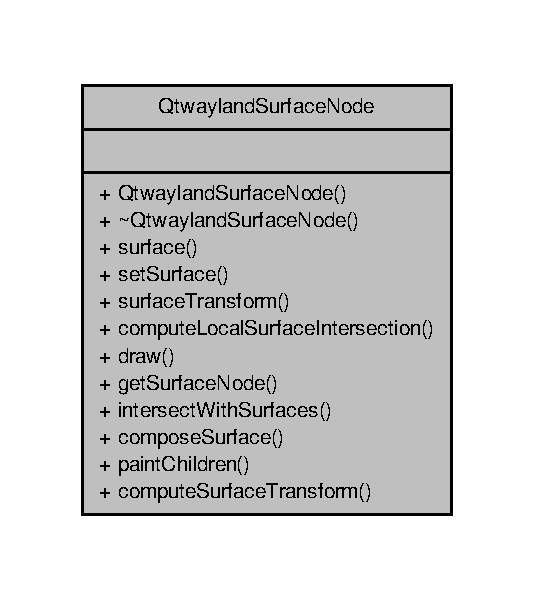
\includegraphics[width=256pt]{classQtwaylandSurfaceNode__coll__graph}
\end{center}
\end{figure}
\subsection*{Public Member Functions}
\begin{DoxyCompactItemize}
\item 
\hyperlink{classQtwaylandSurfaceNode_a582fc9fb7bee6fecc1935c229bc84e72}{Qtwayland\-Surface\-Node} (Q\-Object $\ast$parent, Q\-Wayland\-Surface $\ast$\hyperlink{classQtwaylandSurfaceNode_a8f07c78202a2faa244d9d6c389c03951}{surface}, glm\-::mat4 transform=glm\-::mat4(1))
\item 
virtual \hyperlink{classQtwaylandSurfaceNode_af762332b319b9239e955d4a69b165c14}{$\sim$\-Qtwayland\-Surface\-Node} ()
\item 
Q\-Wayland\-Surface $\ast$ \hyperlink{classQtwaylandSurfaceNode_a8f07c78202a2faa244d9d6c389c03951}{surface} () const 
\item 
void \hyperlink{classQtwaylandSurfaceNode_ace08a2691d01fe10087e9b6997d1523b}{set\-Surface} (Q\-Wayland\-Surface $\ast$\hyperlink{classQtwaylandSurfaceNode_a8f07c78202a2faa244d9d6c389c03951}{surface})
\item 
glm\-::mat4 \hyperlink{classQtwaylandSurfaceNode_a8f88e9c392012d312206da67d6ea81ed}{surface\-Transform} () const 
\item 
bool \hyperlink{classQtwaylandSurfaceNode_a0307e078cfa9bcd6aaad60830ab5b3a6}{compute\-Local\-Surface\-Intersection} (const Geometry\-::\-Ray \&local\-Ray, Q\-Point\-F \&local\-Intersection, float \&t) const 
\item 
virtual bool \hyperlink{classQtwaylandSurfaceNode_a620c58196d857fe5146cfff49c6787fd}{draw} (Display\-Node $\ast$display)
\item 
virtual \hyperlink{classQtwaylandSurfaceNode}{Qtwayland\-Surface\-Node} $\ast$ \hyperlink{classQtwaylandSurfaceNode_a72db2bcd85e26d7f0332175f691a0dfd}{get\-Surface\-Node} (const Q\-Wayland\-Surface $\ast$\hyperlink{classQtwaylandSurfaceNode_a8f07c78202a2faa244d9d6c389c03951}{surface}=N\-U\-L\-L)
\item 
virtual \\*
Scene\-Graph\-Node\-::\-Ray\-Surface\-Intersection $\ast$ \hyperlink{classQtwaylandSurfaceNode_a82a9f9f93675df011cfd350a1857ea8b}{intersect\-With\-Surfaces} (const Geometry\-::\-Ray \&ray)
\item 
G\-Luint \hyperlink{classQtwaylandSurfaceNode_a16ad301303ca42fa9a2ad3d1799cf1a2}{compose\-Surface} (Q\-Wayland\-Surface $\ast$\hyperlink{classQtwaylandSurfaceNode_a8f07c78202a2faa244d9d6c389c03951}{surface}, \hyperlink{classOpenGLData}{Open\-G\-L\-Data} $\ast$gl\-Data)
\item 
void \hyperlink{classQtwaylandSurfaceNode_a0de0e4cbe5312d91334e091160ac4bce}{paint\-Children} (Q\-Wayland\-Surface $\ast$\hyperlink{classQtwaylandSurfaceNode_a8f07c78202a2faa244d9d6c389c03951}{surface}, Q\-Wayland\-Surface $\ast$window, \hyperlink{classOpenGLData}{Open\-G\-L\-Data} $\ast$gl\-Data)
\item 
void \hyperlink{classQtwaylandSurfaceNode_a9917572c6241c4a7593b4c9cd9f8c290}{compute\-Surface\-Transform} (float ppcm)
\end{DoxyCompactItemize}


\subsection{Constructor \& Destructor Documentation}
\hypertarget{classQtwaylandSurfaceNode_a582fc9fb7bee6fecc1935c229bc84e72}{\index{Qtwayland\-Surface\-Node@{Qtwayland\-Surface\-Node}!Qtwayland\-Surface\-Node@{Qtwayland\-Surface\-Node}}
\index{Qtwayland\-Surface\-Node@{Qtwayland\-Surface\-Node}!QtwaylandSurfaceNode@{Qtwayland\-Surface\-Node}}
\subsubsection[{Qtwayland\-Surface\-Node}]{\setlength{\rightskip}{0pt plus 5cm}Qtwayland\-Surface\-Node\-::\-Qtwayland\-Surface\-Node (
\begin{DoxyParamCaption}
\item[{Q\-Object $\ast$}]{parent, }
\item[{Q\-Wayland\-Surface $\ast$}]{surface, }
\item[{glm\-::mat4}]{transform = {\ttfamily glm\-:\-:mat4(1)}}
\end{DoxyParamCaption}
)}}\label{classQtwaylandSurfaceNode_a582fc9fb7bee6fecc1935c229bc84e72}
\hypertarget{classQtwaylandSurfaceNode_af762332b319b9239e955d4a69b165c14}{\index{Qtwayland\-Surface\-Node@{Qtwayland\-Surface\-Node}!$\sim$\-Qtwayland\-Surface\-Node@{$\sim$\-Qtwayland\-Surface\-Node}}
\index{$\sim$\-Qtwayland\-Surface\-Node@{$\sim$\-Qtwayland\-Surface\-Node}!QtwaylandSurfaceNode@{Qtwayland\-Surface\-Node}}
\subsubsection[{$\sim$\-Qtwayland\-Surface\-Node}]{\setlength{\rightskip}{0pt plus 5cm}Qtwayland\-Surface\-Node\-::$\sim$\-Qtwayland\-Surface\-Node (
\begin{DoxyParamCaption}
{}
\end{DoxyParamCaption}
)\hspace{0.3cm}{\ttfamily [virtual]}}}\label{classQtwaylandSurfaceNode_af762332b319b9239e955d4a69b165c14}


\subsection{Member Function Documentation}
\hypertarget{classQtwaylandSurfaceNode_a16ad301303ca42fa9a2ad3d1799cf1a2}{\index{Qtwayland\-Surface\-Node@{Qtwayland\-Surface\-Node}!compose\-Surface@{compose\-Surface}}
\index{compose\-Surface@{compose\-Surface}!QtwaylandSurfaceNode@{Qtwayland\-Surface\-Node}}
\subsubsection[{compose\-Surface}]{\setlength{\rightskip}{0pt plus 5cm}G\-Luint Qtwayland\-Surface\-Node\-::compose\-Surface (
\begin{DoxyParamCaption}
\item[{Q\-Wayland\-Surface $\ast$}]{surface, }
\item[{{\bf Open\-G\-L\-Data} $\ast$}]{gl\-Data}
\end{DoxyParamCaption}
)}}\label{classQtwaylandSurfaceNode_a16ad301303ca42fa9a2ad3d1799cf1a2}
\hypertarget{classQtwaylandSurfaceNode_a0307e078cfa9bcd6aaad60830ab5b3a6}{\index{Qtwayland\-Surface\-Node@{Qtwayland\-Surface\-Node}!compute\-Local\-Surface\-Intersection@{compute\-Local\-Surface\-Intersection}}
\index{compute\-Local\-Surface\-Intersection@{compute\-Local\-Surface\-Intersection}!QtwaylandSurfaceNode@{Qtwayland\-Surface\-Node}}
\subsubsection[{compute\-Local\-Surface\-Intersection}]{\setlength{\rightskip}{0pt plus 5cm}bool Qtwayland\-Surface\-Node\-::compute\-Local\-Surface\-Intersection (
\begin{DoxyParamCaption}
\item[{const Geometry\-::\-Ray \&}]{local\-Ray, }
\item[{Q\-Point\-F \&}]{local\-Intersection, }
\item[{float \&}]{t}
\end{DoxyParamCaption}
) const}}\label{classQtwaylandSurfaceNode_a0307e078cfa9bcd6aaad60830ab5b3a6}
\hypertarget{classQtwaylandSurfaceNode_a9917572c6241c4a7593b4c9cd9f8c290}{\index{Qtwayland\-Surface\-Node@{Qtwayland\-Surface\-Node}!compute\-Surface\-Transform@{compute\-Surface\-Transform}}
\index{compute\-Surface\-Transform@{compute\-Surface\-Transform}!QtwaylandSurfaceNode@{Qtwayland\-Surface\-Node}}
\subsubsection[{compute\-Surface\-Transform}]{\setlength{\rightskip}{0pt plus 5cm}void Qtwayland\-Surface\-Node\-::compute\-Surface\-Transform (
\begin{DoxyParamCaption}
\item[{float}]{ppcm}
\end{DoxyParamCaption}
)}}\label{classQtwaylandSurfaceNode_a9917572c6241c4a7593b4c9cd9f8c290}
\hypertarget{classQtwaylandSurfaceNode_a620c58196d857fe5146cfff49c6787fd}{\index{Qtwayland\-Surface\-Node@{Qtwayland\-Surface\-Node}!draw@{draw}}
\index{draw@{draw}!QtwaylandSurfaceNode@{Qtwayland\-Surface\-Node}}
\subsubsection[{draw}]{\setlength{\rightskip}{0pt plus 5cm}bool Qtwayland\-Surface\-Node\-::draw (
\begin{DoxyParamCaption}
\item[{Display\-Node $\ast$}]{display}
\end{DoxyParamCaption}
)\hspace{0.3cm}{\ttfamily [virtual]}}}\label{classQtwaylandSurfaceNode_a620c58196d857fe5146cfff49c6787fd}
\hypertarget{classQtwaylandSurfaceNode_a72db2bcd85e26d7f0332175f691a0dfd}{\index{Qtwayland\-Surface\-Node@{Qtwayland\-Surface\-Node}!get\-Surface\-Node@{get\-Surface\-Node}}
\index{get\-Surface\-Node@{get\-Surface\-Node}!QtwaylandSurfaceNode@{Qtwayland\-Surface\-Node}}
\subsubsection[{get\-Surface\-Node}]{\setlength{\rightskip}{0pt plus 5cm}{\bf Qtwayland\-Surface\-Node} $\ast$ Qtwayland\-Surface\-Node\-::get\-Surface\-Node (
\begin{DoxyParamCaption}
\item[{const Q\-Wayland\-Surface $\ast$}]{surface = {\ttfamily NULL}}
\end{DoxyParamCaption}
)\hspace{0.3cm}{\ttfamily [virtual]}}}\label{classQtwaylandSurfaceNode_a72db2bcd85e26d7f0332175f691a0dfd}
\hypertarget{classQtwaylandSurfaceNode_a82a9f9f93675df011cfd350a1857ea8b}{\index{Qtwayland\-Surface\-Node@{Qtwayland\-Surface\-Node}!intersect\-With\-Surfaces@{intersect\-With\-Surfaces}}
\index{intersect\-With\-Surfaces@{intersect\-With\-Surfaces}!QtwaylandSurfaceNode@{Qtwayland\-Surface\-Node}}
\subsubsection[{intersect\-With\-Surfaces}]{\setlength{\rightskip}{0pt plus 5cm}Scene\-Graph\-Node\-::\-Ray\-Surface\-Intersection $\ast$ Qtwayland\-Surface\-Node\-::intersect\-With\-Surfaces (
\begin{DoxyParamCaption}
\item[{const Geometry\-::\-Ray \&}]{ray}
\end{DoxyParamCaption}
)\hspace{0.3cm}{\ttfamily [virtual]}}}\label{classQtwaylandSurfaceNode_a82a9f9f93675df011cfd350a1857ea8b}
\hypertarget{classQtwaylandSurfaceNode_a0de0e4cbe5312d91334e091160ac4bce}{\index{Qtwayland\-Surface\-Node@{Qtwayland\-Surface\-Node}!paint\-Children@{paint\-Children}}
\index{paint\-Children@{paint\-Children}!QtwaylandSurfaceNode@{Qtwayland\-Surface\-Node}}
\subsubsection[{paint\-Children}]{\setlength{\rightskip}{0pt plus 5cm}void Qtwayland\-Surface\-Node\-::paint\-Children (
\begin{DoxyParamCaption}
\item[{Q\-Wayland\-Surface $\ast$}]{surface, }
\item[{Q\-Wayland\-Surface $\ast$}]{window, }
\item[{{\bf Open\-G\-L\-Data} $\ast$}]{gl\-Data}
\end{DoxyParamCaption}
)}}\label{classQtwaylandSurfaceNode_a0de0e4cbe5312d91334e091160ac4bce}
\hypertarget{classQtwaylandSurfaceNode_ace08a2691d01fe10087e9b6997d1523b}{\index{Qtwayland\-Surface\-Node@{Qtwayland\-Surface\-Node}!set\-Surface@{set\-Surface}}
\index{set\-Surface@{set\-Surface}!QtwaylandSurfaceNode@{Qtwayland\-Surface\-Node}}
\subsubsection[{set\-Surface}]{\setlength{\rightskip}{0pt plus 5cm}void Qtwayland\-Surface\-Node\-::set\-Surface (
\begin{DoxyParamCaption}
\item[{Q\-Wayland\-Surface $\ast$}]{surface}
\end{DoxyParamCaption}
)}}\label{classQtwaylandSurfaceNode_ace08a2691d01fe10087e9b6997d1523b}
\hypertarget{classQtwaylandSurfaceNode_a8f07c78202a2faa244d9d6c389c03951}{\index{Qtwayland\-Surface\-Node@{Qtwayland\-Surface\-Node}!surface@{surface}}
\index{surface@{surface}!QtwaylandSurfaceNode@{Qtwayland\-Surface\-Node}}
\subsubsection[{surface}]{\setlength{\rightskip}{0pt plus 5cm}Q\-Wayland\-Surface $\ast$ Qtwayland\-Surface\-Node\-::surface (
\begin{DoxyParamCaption}
{}
\end{DoxyParamCaption}
) const}}\label{classQtwaylandSurfaceNode_a8f07c78202a2faa244d9d6c389c03951}
\hypertarget{classQtwaylandSurfaceNode_a8f88e9c392012d312206da67d6ea81ed}{\index{Qtwayland\-Surface\-Node@{Qtwayland\-Surface\-Node}!surface\-Transform@{surface\-Transform}}
\index{surface\-Transform@{surface\-Transform}!QtwaylandSurfaceNode@{Qtwayland\-Surface\-Node}}
\subsubsection[{surface\-Transform}]{\setlength{\rightskip}{0pt plus 5cm}glm\-::mat4 Qtwayland\-Surface\-Node\-::surface\-Transform (
\begin{DoxyParamCaption}
{}
\end{DoxyParamCaption}
) const}}\label{classQtwaylandSurfaceNode_a8f88e9c392012d312206da67d6ea81ed}


The documentation for this class was generated from the following files\-:\begin{DoxyCompactItemize}
\item 
/home/dave/thesis/qtwayland-\/motorcar-\/compositor/qt/src/\hyperlink{qtwaylandsurfacenode_8h}{qtwaylandsurfacenode.\-h}\item 
/home/dave/thesis/qtwayland-\/motorcar-\/compositor/qt/src/\hyperlink{qtwaylandsurfacenode_8cpp}{qtwaylandsurfacenode.\-cpp}\end{DoxyCompactItemize}

\hypertarget{structmotorcar_1_1Geometry_1_1Ray}{\section{motorcar\-:\-:Geometry\-:\-:Ray Struct Reference}
\label{structmotorcar_1_1Geometry_1_1Ray}\index{motorcar\-::\-Geometry\-::\-Ray@{motorcar\-::\-Geometry\-::\-Ray}}
}


{\ttfamily \#include $<$geometry.\-h$>$}

\subsection*{Public Member Functions}
\begin{DoxyCompactItemize}
\item 
\hyperlink{structmotorcar_1_1Geometry_1_1Ray_a0e703633f6101262ee14d17831745ca4}{Ray} (glm\-::vec3 \hyperlink{structmotorcar_1_1Geometry_1_1Ray_ac58960f9f82f19c6f514ae6c948deb86}{p}, glm\-::vec3 \hyperlink{structmotorcar_1_1Geometry_1_1Ray_a7140db28237277781ecb792fc280a95d}{d})
\item 
\hyperlink{structmotorcar_1_1Geometry_1_1Ray}{Ray} \hyperlink{structmotorcar_1_1Geometry_1_1Ray_a7de7ddd9609a26bdd1f2fe74933dfff6}{transform} (glm\-::mat4 t) const 
\item 
glm\-::vec3 \hyperlink{structmotorcar_1_1Geometry_1_1Ray_af14d102bfe9fdf08bb3396ad33d928bd}{solve} (float t) const 
\item 
void \hyperlink{structmotorcar_1_1Geometry_1_1Ray_a058da6e22e8fdcd7e2aa301153c9fa16}{print} () const 
\item 
void \hyperlink{structmotorcar_1_1Geometry_1_1Ray_a7d9403aa28c33c40d4b7e3c64ce3776d}{draw} (\hyperlink{classmotorcar_1_1SceneGraphNode}{motorcar\-::\-Scene\-Graph\-Node} $\ast$parent, glm\-::vec3 color, glm\-::mat4 \hyperlink{structmotorcar_1_1Geometry_1_1Ray_a7de7ddd9609a26bdd1f2fe74933dfff6}{transform}=glm\-::mat4(1))
\end{DoxyCompactItemize}
\subsection*{Public Attributes}
\begin{DoxyCompactItemize}
\item 
glm\-::vec3 \hyperlink{structmotorcar_1_1Geometry_1_1Ray_ac58960f9f82f19c6f514ae6c948deb86}{p}
\item 
glm\-::vec3 \hyperlink{structmotorcar_1_1Geometry_1_1Ray_a7140db28237277781ecb792fc280a95d}{d}
\end{DoxyCompactItemize}


\subsection{Constructor \& Destructor Documentation}
\hypertarget{structmotorcar_1_1Geometry_1_1Ray_a0e703633f6101262ee14d17831745ca4}{\index{motorcar\-::\-Geometry\-::\-Ray@{motorcar\-::\-Geometry\-::\-Ray}!Ray@{Ray}}
\index{Ray@{Ray}!motorcar::Geometry::Ray@{motorcar\-::\-Geometry\-::\-Ray}}
\subsubsection[{Ray}]{\setlength{\rightskip}{0pt plus 5cm}Geometry\-::\-Ray\-::\-Ray (
\begin{DoxyParamCaption}
\item[{glm\-::vec3}]{p, }
\item[{glm\-::vec3}]{d}
\end{DoxyParamCaption}
)}}\label{structmotorcar_1_1Geometry_1_1Ray_a0e703633f6101262ee14d17831745ca4}


\subsection{Member Function Documentation}
\hypertarget{structmotorcar_1_1Geometry_1_1Ray_a7d9403aa28c33c40d4b7e3c64ce3776d}{\index{motorcar\-::\-Geometry\-::\-Ray@{motorcar\-::\-Geometry\-::\-Ray}!draw@{draw}}
\index{draw@{draw}!motorcar::Geometry::Ray@{motorcar\-::\-Geometry\-::\-Ray}}
\subsubsection[{draw}]{\setlength{\rightskip}{0pt plus 5cm}void Geometry\-::\-Ray\-::draw (
\begin{DoxyParamCaption}
\item[{{\bf motorcar\-::\-Scene\-Graph\-Node} $\ast$}]{parent, }
\item[{glm\-::vec3}]{color, }
\item[{glm\-::mat4}]{transform = {\ttfamily glm\-:\-:mat4(1)}}
\end{DoxyParamCaption}
)}}\label{structmotorcar_1_1Geometry_1_1Ray_a7d9403aa28c33c40d4b7e3c64ce3776d}
\hypertarget{structmotorcar_1_1Geometry_1_1Ray_a058da6e22e8fdcd7e2aa301153c9fa16}{\index{motorcar\-::\-Geometry\-::\-Ray@{motorcar\-::\-Geometry\-::\-Ray}!print@{print}}
\index{print@{print}!motorcar::Geometry::Ray@{motorcar\-::\-Geometry\-::\-Ray}}
\subsubsection[{print}]{\setlength{\rightskip}{0pt plus 5cm}void Geometry\-::\-Ray\-::print (
\begin{DoxyParamCaption}
{}
\end{DoxyParamCaption}
) const}}\label{structmotorcar_1_1Geometry_1_1Ray_a058da6e22e8fdcd7e2aa301153c9fa16}
\hypertarget{structmotorcar_1_1Geometry_1_1Ray_af14d102bfe9fdf08bb3396ad33d928bd}{\index{motorcar\-::\-Geometry\-::\-Ray@{motorcar\-::\-Geometry\-::\-Ray}!solve@{solve}}
\index{solve@{solve}!motorcar::Geometry::Ray@{motorcar\-::\-Geometry\-::\-Ray}}
\subsubsection[{solve}]{\setlength{\rightskip}{0pt plus 5cm}glm\-::vec3 Geometry\-::\-Ray\-::solve (
\begin{DoxyParamCaption}
\item[{float}]{t}
\end{DoxyParamCaption}
) const}}\label{structmotorcar_1_1Geometry_1_1Ray_af14d102bfe9fdf08bb3396ad33d928bd}
\hypertarget{structmotorcar_1_1Geometry_1_1Ray_a7de7ddd9609a26bdd1f2fe74933dfff6}{\index{motorcar\-::\-Geometry\-::\-Ray@{motorcar\-::\-Geometry\-::\-Ray}!transform@{transform}}
\index{transform@{transform}!motorcar::Geometry::Ray@{motorcar\-::\-Geometry\-::\-Ray}}
\subsubsection[{transform}]{\setlength{\rightskip}{0pt plus 5cm}{\bf Geometry\-::\-Ray} Geometry\-::\-Ray\-::transform (
\begin{DoxyParamCaption}
\item[{glm\-::mat4}]{t}
\end{DoxyParamCaption}
) const}}\label{structmotorcar_1_1Geometry_1_1Ray_a7de7ddd9609a26bdd1f2fe74933dfff6}


\subsection{Member Data Documentation}
\hypertarget{structmotorcar_1_1Geometry_1_1Ray_a7140db28237277781ecb792fc280a95d}{\index{motorcar\-::\-Geometry\-::\-Ray@{motorcar\-::\-Geometry\-::\-Ray}!d@{d}}
\index{d@{d}!motorcar::Geometry::Ray@{motorcar\-::\-Geometry\-::\-Ray}}
\subsubsection[{d}]{\setlength{\rightskip}{0pt plus 5cm}glm\-::vec3 motorcar\-::\-Geometry\-::\-Ray\-::d}}\label{structmotorcar_1_1Geometry_1_1Ray_a7140db28237277781ecb792fc280a95d}
\hypertarget{structmotorcar_1_1Geometry_1_1Ray_ac58960f9f82f19c6f514ae6c948deb86}{\index{motorcar\-::\-Geometry\-::\-Ray@{motorcar\-::\-Geometry\-::\-Ray}!p@{p}}
\index{p@{p}!motorcar::Geometry::Ray@{motorcar\-::\-Geometry\-::\-Ray}}
\subsubsection[{p}]{\setlength{\rightskip}{0pt plus 5cm}glm\-::vec3 motorcar\-::\-Geometry\-::\-Ray\-::p}}\label{structmotorcar_1_1Geometry_1_1Ray_ac58960f9f82f19c6f514ae6c948deb86}


The documentation for this struct was generated from the following files\-:\begin{DoxyCompactItemize}
\item 
/home/dave/thesis/motorcar/src/compositor/\hyperlink{geometry_8h}{geometry.\-h}\item 
/home/dave/thesis/motorcar/src/compositor/\hyperlink{geometry_8cpp}{geometry.\-cpp}\end{DoxyCompactItemize}

\hypertarget{structmotorcar_1_1Geometry_1_1RaySurfaceIntersection}{\section{motorcar\-:\-:Geometry\-:\-:Ray\-Surface\-Intersection Struct Reference}
\label{structmotorcar_1_1Geometry_1_1RaySurfaceIntersection}\index{motorcar\-::\-Geometry\-::\-Ray\-Surface\-Intersection@{motorcar\-::\-Geometry\-::\-Ray\-Surface\-Intersection}}
}


{\ttfamily \#include $<$geometry.\-h$>$}



Collaboration diagram for motorcar\-:\-:Geometry\-:\-:Ray\-Surface\-Intersection\-:
\nopagebreak
\begin{figure}[H]
\begin{center}
\leavevmode
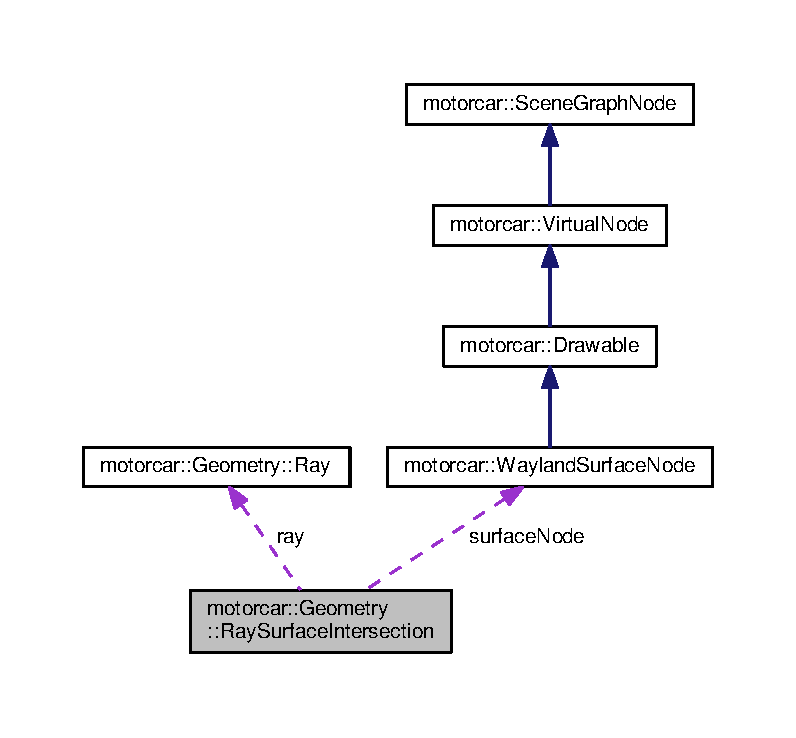
\includegraphics[height=550pt]{structmotorcar_1_1Geometry_1_1RaySurfaceIntersection__coll__graph}
\end{center}
\end{figure}
\subsection*{Public Member Functions}
\begin{DoxyCompactItemize}
\item 
\hyperlink{structmotorcar_1_1Geometry_1_1RaySurfaceIntersection_a25998175e122ecae30e93f823b3b84e4}{Ray\-Surface\-Intersection} (\hyperlink{classmotorcar_1_1WaylandSurfaceNode}{Wayland\-Surface\-Node} $\ast$\hyperlink{structmotorcar_1_1Geometry_1_1RaySurfaceIntersection_aaea662da642316b521721a5dcff0a280}{surface\-Node}, glm\-::vec2 \hyperlink{structmotorcar_1_1Geometry_1_1RaySurfaceIntersection_abb64ad1bdb4385d23970b1c7ecd4afaa}{surface\-Local\-Coordinates}, const \hyperlink{structmotorcar_1_1Geometry_1_1Ray}{Geometry\-::\-Ray} \&\hyperlink{structmotorcar_1_1Geometry_1_1RaySurfaceIntersection_a2e53423ad071c4587aac822ee6aa3de9}{ray}, float \hyperlink{structmotorcar_1_1Geometry_1_1RaySurfaceIntersection_af32545772aead85519b20869fbc34284}{t})
\end{DoxyCompactItemize}
\subsection*{Public Attributes}
\begin{DoxyCompactItemize}
\item 
\hyperlink{classmotorcar_1_1WaylandSurfaceNode}{Wayland\-Surface\-Node} $\ast$ \hyperlink{structmotorcar_1_1Geometry_1_1RaySurfaceIntersection_aaea662da642316b521721a5dcff0a280}{surface\-Node}
\item 
glm\-::vec2 \hyperlink{structmotorcar_1_1Geometry_1_1RaySurfaceIntersection_abb64ad1bdb4385d23970b1c7ecd4afaa}{surface\-Local\-Coordinates}
\item 
\hyperlink{structmotorcar_1_1Geometry_1_1Ray}{Geometry\-::\-Ray} \hyperlink{structmotorcar_1_1Geometry_1_1RaySurfaceIntersection_a2e53423ad071c4587aac822ee6aa3de9}{ray}
\item 
float \hyperlink{structmotorcar_1_1Geometry_1_1RaySurfaceIntersection_af32545772aead85519b20869fbc34284}{t}
\end{DoxyCompactItemize}


\subsection{Constructor \& Destructor Documentation}
\hypertarget{structmotorcar_1_1Geometry_1_1RaySurfaceIntersection_a25998175e122ecae30e93f823b3b84e4}{\index{motorcar\-::\-Geometry\-::\-Ray\-Surface\-Intersection@{motorcar\-::\-Geometry\-::\-Ray\-Surface\-Intersection}!Ray\-Surface\-Intersection@{Ray\-Surface\-Intersection}}
\index{Ray\-Surface\-Intersection@{Ray\-Surface\-Intersection}!motorcar::Geometry::RaySurfaceIntersection@{motorcar\-::\-Geometry\-::\-Ray\-Surface\-Intersection}}
\subsubsection[{Ray\-Surface\-Intersection}]{\setlength{\rightskip}{0pt plus 5cm}Geometry\-::\-Ray\-Surface\-Intersection\-::\-Ray\-Surface\-Intersection (
\begin{DoxyParamCaption}
\item[{{\bf Wayland\-Surface\-Node} $\ast$}]{surface\-Node, }
\item[{glm\-::vec2}]{surface\-Local\-Coordinates, }
\item[{const {\bf Geometry\-::\-Ray} \&}]{ray, }
\item[{float}]{t}
\end{DoxyParamCaption}
)}}\label{structmotorcar_1_1Geometry_1_1RaySurfaceIntersection_a25998175e122ecae30e93f823b3b84e4}


\subsection{Member Data Documentation}
\hypertarget{structmotorcar_1_1Geometry_1_1RaySurfaceIntersection_a2e53423ad071c4587aac822ee6aa3de9}{\index{motorcar\-::\-Geometry\-::\-Ray\-Surface\-Intersection@{motorcar\-::\-Geometry\-::\-Ray\-Surface\-Intersection}!ray@{ray}}
\index{ray@{ray}!motorcar::Geometry::RaySurfaceIntersection@{motorcar\-::\-Geometry\-::\-Ray\-Surface\-Intersection}}
\subsubsection[{ray}]{\setlength{\rightskip}{0pt plus 5cm}{\bf Geometry\-::\-Ray} motorcar\-::\-Geometry\-::\-Ray\-Surface\-Intersection\-::ray}}\label{structmotorcar_1_1Geometry_1_1RaySurfaceIntersection_a2e53423ad071c4587aac822ee6aa3de9}
\hypertarget{structmotorcar_1_1Geometry_1_1RaySurfaceIntersection_abb64ad1bdb4385d23970b1c7ecd4afaa}{\index{motorcar\-::\-Geometry\-::\-Ray\-Surface\-Intersection@{motorcar\-::\-Geometry\-::\-Ray\-Surface\-Intersection}!surface\-Local\-Coordinates@{surface\-Local\-Coordinates}}
\index{surface\-Local\-Coordinates@{surface\-Local\-Coordinates}!motorcar::Geometry::RaySurfaceIntersection@{motorcar\-::\-Geometry\-::\-Ray\-Surface\-Intersection}}
\subsubsection[{surface\-Local\-Coordinates}]{\setlength{\rightskip}{0pt plus 5cm}glm\-::vec2 motorcar\-::\-Geometry\-::\-Ray\-Surface\-Intersection\-::surface\-Local\-Coordinates}}\label{structmotorcar_1_1Geometry_1_1RaySurfaceIntersection_abb64ad1bdb4385d23970b1c7ecd4afaa}
\hypertarget{structmotorcar_1_1Geometry_1_1RaySurfaceIntersection_aaea662da642316b521721a5dcff0a280}{\index{motorcar\-::\-Geometry\-::\-Ray\-Surface\-Intersection@{motorcar\-::\-Geometry\-::\-Ray\-Surface\-Intersection}!surface\-Node@{surface\-Node}}
\index{surface\-Node@{surface\-Node}!motorcar::Geometry::RaySurfaceIntersection@{motorcar\-::\-Geometry\-::\-Ray\-Surface\-Intersection}}
\subsubsection[{surface\-Node}]{\setlength{\rightskip}{0pt plus 5cm}{\bf Wayland\-Surface\-Node}$\ast$ motorcar\-::\-Geometry\-::\-Ray\-Surface\-Intersection\-::surface\-Node}}\label{structmotorcar_1_1Geometry_1_1RaySurfaceIntersection_aaea662da642316b521721a5dcff0a280}
\hypertarget{structmotorcar_1_1Geometry_1_1RaySurfaceIntersection_af32545772aead85519b20869fbc34284}{\index{motorcar\-::\-Geometry\-::\-Ray\-Surface\-Intersection@{motorcar\-::\-Geometry\-::\-Ray\-Surface\-Intersection}!t@{t}}
\index{t@{t}!motorcar::Geometry::RaySurfaceIntersection@{motorcar\-::\-Geometry\-::\-Ray\-Surface\-Intersection}}
\subsubsection[{t}]{\setlength{\rightskip}{0pt plus 5cm}float motorcar\-::\-Geometry\-::\-Ray\-Surface\-Intersection\-::t}}\label{structmotorcar_1_1Geometry_1_1RaySurfaceIntersection_af32545772aead85519b20869fbc34284}


The documentation for this struct was generated from the following files\-:\begin{DoxyCompactItemize}
\item 
/home/dave/thesis/qtwayland-\/motorcar-\/compositor/motorcar/src/\hyperlink{geometry_8h}{geometry.\-h}\item 
/home/dave/thesis/qtwayland-\/motorcar-\/compositor/motorcar/src/\hyperlink{geometry_8cpp}{geometry.\-cpp}\end{DoxyCompactItemize}

\hypertarget{structmotorcar_1_1Geometry_1_1Rectangle}{\section{motorcar\-:\-:Geometry\-:\-:Rectangle Struct Reference}
\label{structmotorcar_1_1Geometry_1_1Rectangle}\index{motorcar\-::\-Geometry\-::\-Rectangle@{motorcar\-::\-Geometry\-::\-Rectangle}}
}


{\ttfamily \#include $<$geometry.\-h$>$}



Inheritance diagram for motorcar\-:\-:Geometry\-:\-:Rectangle\-:
\nopagebreak
\begin{figure}[H]
\begin{center}
\leavevmode
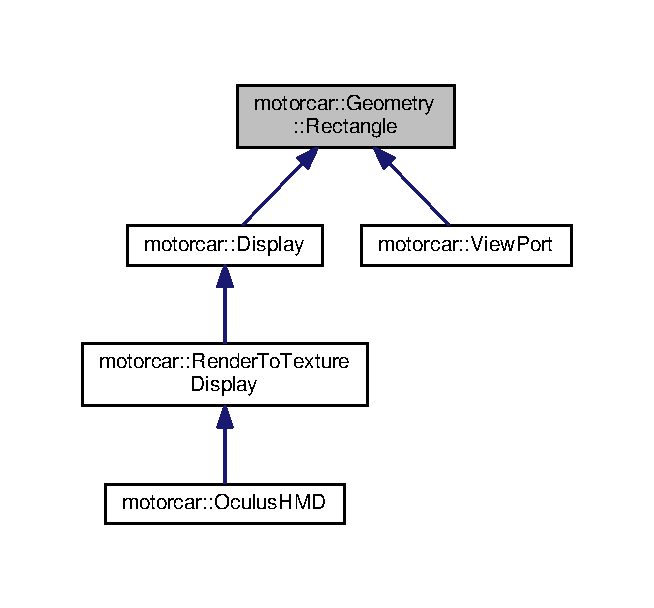
\includegraphics[width=314pt]{structmotorcar_1_1Geometry_1_1Rectangle__inherit__graph}
\end{center}
\end{figure}
\subsection*{Public Member Functions}
\begin{DoxyCompactItemize}
\item 
\hyperlink{structmotorcar_1_1Geometry_1_1Rectangle_af8ec2dc746ed046045d14d31a4973b2e}{Rectangle} (glm\-::ivec2 \hyperlink{structmotorcar_1_1Geometry_1_1Rectangle_aef0385032dd32c2b2c762c08f1bfacf6}{size})
\item 
\hyperlink{structmotorcar_1_1Geometry_1_1Rectangle_a3a73665b3e36e9d73968ca77eece4552}{Rectangle} ()
\item 
virtual \hyperlink{structmotorcar_1_1Geometry_1_1Rectangle_aaba0c9f05f24482b1e668a1b63b35fa6}{$\sim$\-Rectangle} ()
\item 
virtual glm\-::ivec2 \hyperlink{structmotorcar_1_1Geometry_1_1Rectangle_aef0385032dd32c2b2c762c08f1bfacf6}{size} ()
\end{DoxyCompactItemize}
\subsection*{Protected Attributes}
\begin{DoxyCompactItemize}
\item 
glm\-::ivec2 \hyperlink{structmotorcar_1_1Geometry_1_1Rectangle_abc1083ea0c3875e6d70d8f11d2909001}{m\-\_\-size}
\end{DoxyCompactItemize}


\subsection{Constructor \& Destructor Documentation}
\hypertarget{structmotorcar_1_1Geometry_1_1Rectangle_af8ec2dc746ed046045d14d31a4973b2e}{\index{motorcar\-::\-Geometry\-::\-Rectangle@{motorcar\-::\-Geometry\-::\-Rectangle}!Rectangle@{Rectangle}}
\index{Rectangle@{Rectangle}!motorcar::Geometry::Rectangle@{motorcar\-::\-Geometry\-::\-Rectangle}}
\subsubsection[{Rectangle}]{\setlength{\rightskip}{0pt plus 5cm}Geometry\-::\-Rectangle\-::\-Rectangle (
\begin{DoxyParamCaption}
\item[{glm\-::ivec2}]{size}
\end{DoxyParamCaption}
)}}\label{structmotorcar_1_1Geometry_1_1Rectangle_af8ec2dc746ed046045d14d31a4973b2e}
\hypertarget{structmotorcar_1_1Geometry_1_1Rectangle_a3a73665b3e36e9d73968ca77eece4552}{\index{motorcar\-::\-Geometry\-::\-Rectangle@{motorcar\-::\-Geometry\-::\-Rectangle}!Rectangle@{Rectangle}}
\index{Rectangle@{Rectangle}!motorcar::Geometry::Rectangle@{motorcar\-::\-Geometry\-::\-Rectangle}}
\subsubsection[{Rectangle}]{\setlength{\rightskip}{0pt plus 5cm}Geometry\-::\-Rectangle\-::\-Rectangle (
\begin{DoxyParamCaption}
{}
\end{DoxyParamCaption}
)}}\label{structmotorcar_1_1Geometry_1_1Rectangle_a3a73665b3e36e9d73968ca77eece4552}
\hypertarget{structmotorcar_1_1Geometry_1_1Rectangle_aaba0c9f05f24482b1e668a1b63b35fa6}{\index{motorcar\-::\-Geometry\-::\-Rectangle@{motorcar\-::\-Geometry\-::\-Rectangle}!$\sim$\-Rectangle@{$\sim$\-Rectangle}}
\index{$\sim$\-Rectangle@{$\sim$\-Rectangle}!motorcar::Geometry::Rectangle@{motorcar\-::\-Geometry\-::\-Rectangle}}
\subsubsection[{$\sim$\-Rectangle}]{\setlength{\rightskip}{0pt plus 5cm}virtual motorcar\-::\-Geometry\-::\-Rectangle\-::$\sim$\-Rectangle (
\begin{DoxyParamCaption}
{}
\end{DoxyParamCaption}
)\hspace{0.3cm}{\ttfamily [inline]}, {\ttfamily [virtual]}}}\label{structmotorcar_1_1Geometry_1_1Rectangle_aaba0c9f05f24482b1e668a1b63b35fa6}


\subsection{Member Function Documentation}
\hypertarget{structmotorcar_1_1Geometry_1_1Rectangle_aef0385032dd32c2b2c762c08f1bfacf6}{\index{motorcar\-::\-Geometry\-::\-Rectangle@{motorcar\-::\-Geometry\-::\-Rectangle}!size@{size}}
\index{size@{size}!motorcar::Geometry::Rectangle@{motorcar\-::\-Geometry\-::\-Rectangle}}
\subsubsection[{size}]{\setlength{\rightskip}{0pt plus 5cm}virtual glm\-::ivec2 motorcar\-::\-Geometry\-::\-Rectangle\-::size (
\begin{DoxyParamCaption}
{}
\end{DoxyParamCaption}
)\hspace{0.3cm}{\ttfamily [inline]}, {\ttfamily [virtual]}}}\label{structmotorcar_1_1Geometry_1_1Rectangle_aef0385032dd32c2b2c762c08f1bfacf6}


Reimplemented in \hyperlink{classmotorcar_1_1Display_a58a94b72684d5b8569a9169591f7613e}{motorcar\-::\-Display}, \hyperlink{classmotorcar_1_1ViewPort_a50e51ee6e264f85f6f0e1c43950e74ce}{motorcar\-::\-View\-Port}, and \hyperlink{classmotorcar_1_1RenderToTextureDisplay_a2e10611cf3fd629a4d962988642ad5b2}{motorcar\-::\-Render\-To\-Texture\-Display}.



\subsection{Member Data Documentation}
\hypertarget{structmotorcar_1_1Geometry_1_1Rectangle_abc1083ea0c3875e6d70d8f11d2909001}{\index{motorcar\-::\-Geometry\-::\-Rectangle@{motorcar\-::\-Geometry\-::\-Rectangle}!m\-\_\-size@{m\-\_\-size}}
\index{m\-\_\-size@{m\-\_\-size}!motorcar::Geometry::Rectangle@{motorcar\-::\-Geometry\-::\-Rectangle}}
\subsubsection[{m\-\_\-size}]{\setlength{\rightskip}{0pt plus 5cm}glm\-::ivec2 motorcar\-::\-Geometry\-::\-Rectangle\-::m\-\_\-size\hspace{0.3cm}{\ttfamily [protected]}}}\label{structmotorcar_1_1Geometry_1_1Rectangle_abc1083ea0c3875e6d70d8f11d2909001}


The documentation for this struct was generated from the following files\-:\begin{DoxyCompactItemize}
\item 
/media/dave/e89b5eb4-\/4b10-\/4edf-\/8ad5-\/0d046a46b978/dave/thesis/qtwayland-\/motorcar-\/compositor/motorcar/src/\hyperlink{geometry_8h}{geometry.\-h}\item 
/media/dave/e89b5eb4-\/4b10-\/4edf-\/8ad5-\/0d046a46b978/dave/thesis/qtwayland-\/motorcar-\/compositor/motorcar/src/\hyperlink{geometry_8cpp}{geometry.\-cpp}\end{DoxyCompactItemize}

\hypertarget{classmotorcar_1_1RenderToTextureDisplay}{\section{motorcar\-:\-:Render\-To\-Texture\-Display Class Reference}
\label{classmotorcar_1_1RenderToTextureDisplay}\index{motorcar\-::\-Render\-To\-Texture\-Display@{motorcar\-::\-Render\-To\-Texture\-Display}}
}


{\ttfamily \#include $<$rendertotexturedisplay.\-h$>$}



Inheritance diagram for motorcar\-:\-:Render\-To\-Texture\-Display\-:
\nopagebreak
\begin{figure}[H]
\begin{center}
\leavevmode
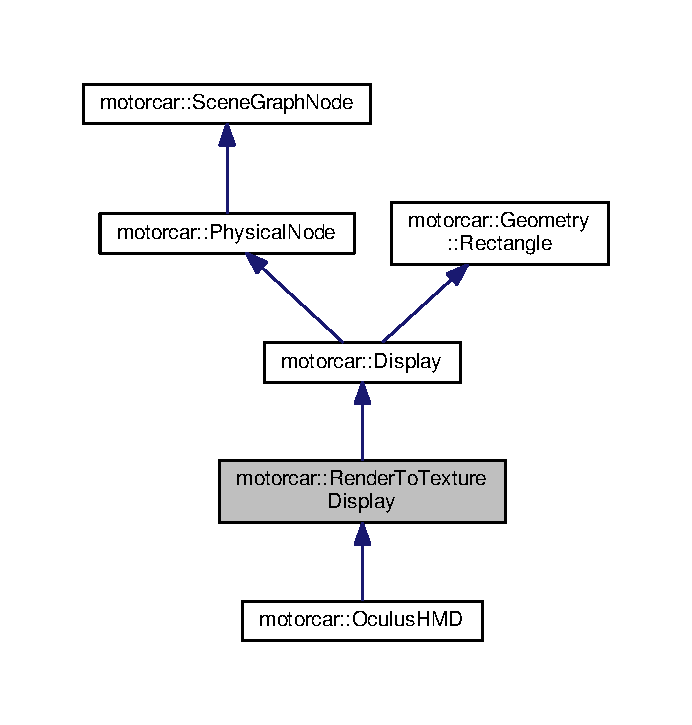
\includegraphics[width=332pt]{classmotorcar_1_1RenderToTextureDisplay__inherit__graph}
\end{center}
\end{figure}


Collaboration diagram for motorcar\-:\-:Render\-To\-Texture\-Display\-:
\nopagebreak
\begin{figure}[H]
\begin{center}
\leavevmode
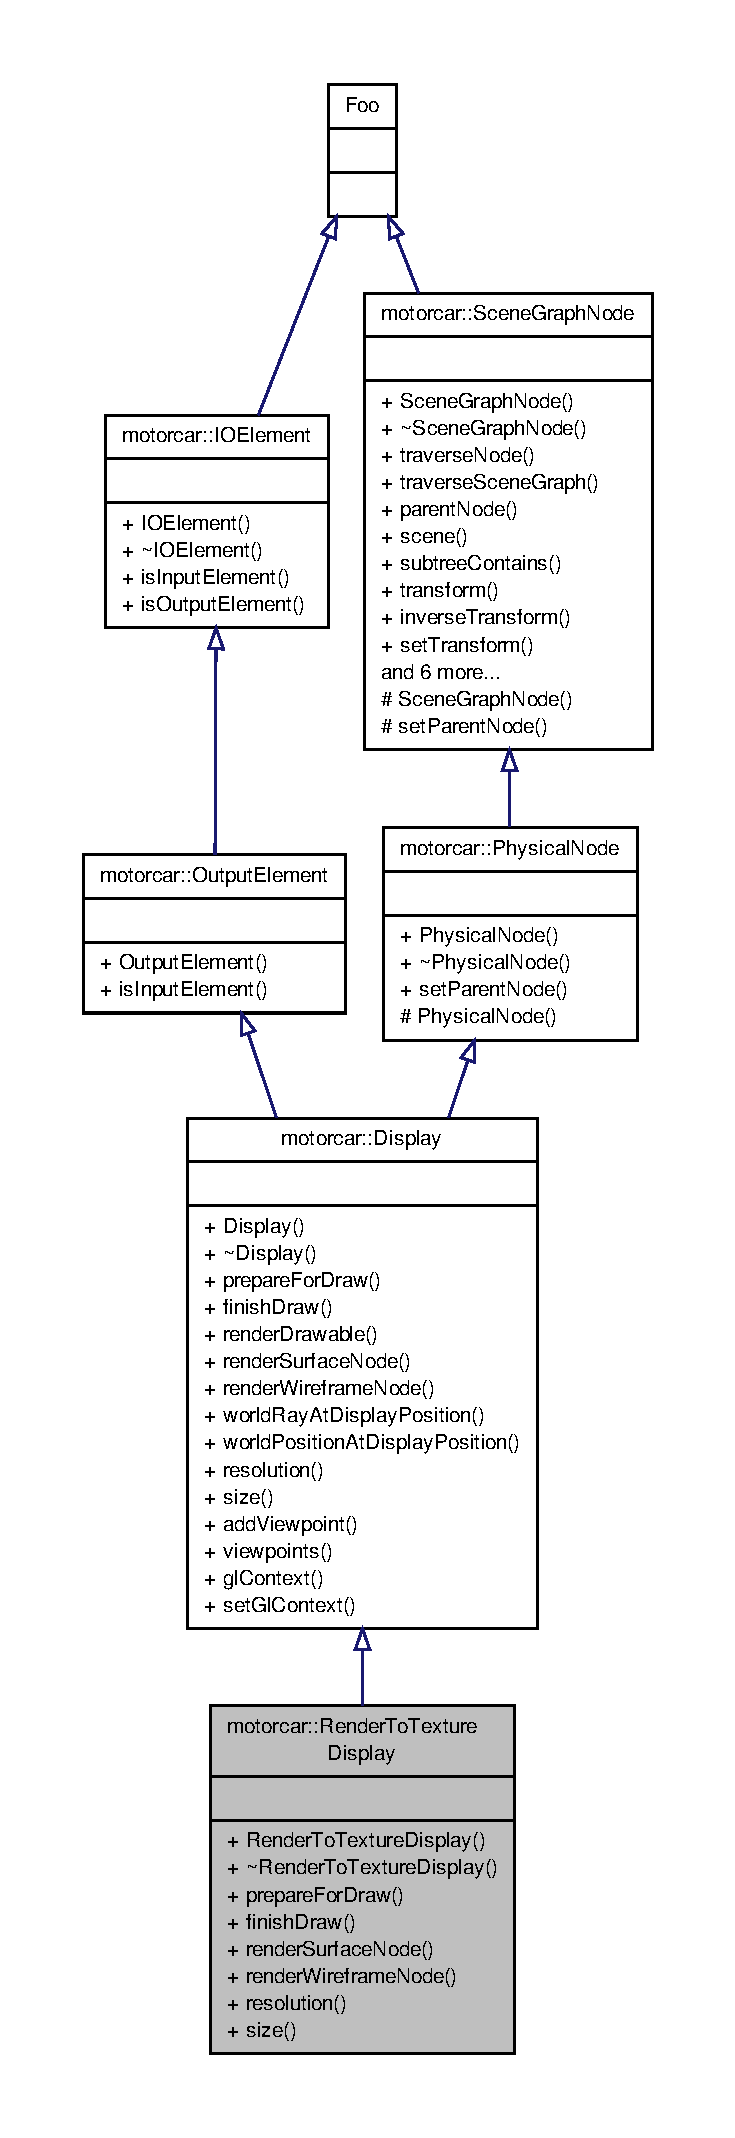
\includegraphics[width=332pt]{classmotorcar_1_1RenderToTextureDisplay__coll__graph}
\end{center}
\end{figure}
\subsection*{Public Member Functions}
\begin{DoxyCompactItemize}
\item 
\hyperlink{classmotorcar_1_1RenderToTextureDisplay_a9c79fc8d2429e8b15c0353a5a9fce42f}{Render\-To\-Texture\-Display} (float scale, glm\-::vec4 distortion\-K, \hyperlink{classmotorcar_1_1OpenGLContext}{Open\-G\-L\-Context} $\ast$\hyperlink{classmotorcar_1_1Display_a884dd0b78dbecee82a33eb6d26a2a403}{gl\-Context}, glm\-::vec2 display\-Dimensions, \hyperlink{classmotorcar_1_1PhysicalNode}{Physical\-Node} $\ast$parent, const glm\-::mat4 \&\hyperlink{classmotorcar_1_1SceneGraphNode_ad96e79fdd739ac8223a3128003be391a}{transform}=glm\-::mat4())
\item 
virtual \hyperlink{classmotorcar_1_1RenderToTextureDisplay_a9cb7b619ef7450f8c208961d83671998}{$\sim$\-Render\-To\-Texture\-Display} ()
\item 
virtual void \hyperlink{classmotorcar_1_1RenderToTextureDisplay_abdf6861fe69ada64fafd0a7713391bed}{prepare\-For\-Draw} () override
\item 
virtual void \hyperlink{classmotorcar_1_1RenderToTextureDisplay_a5a312b98ac49013155797e814e6cf69e}{finish\-Draw} () override
\item 
virtual glm\-::ivec2 \hyperlink{classmotorcar_1_1RenderToTextureDisplay_a2e10611cf3fd629a4d962988642ad5b2}{size} () override
\item 
virtual glm\-::vec2 \hyperlink{classmotorcar_1_1RenderToTextureDisplay_a0ede4d9139786227f2c5d87bbbb9dcfa}{dimensions} () const override
\item 
virtual G\-Luint \hyperlink{classmotorcar_1_1RenderToTextureDisplay_a8c928fb82c28d4785c58a1bd321e0ca6}{active\-Frame\-Buffer} () const override
\item 
virtual G\-Luint \hyperlink{classmotorcar_1_1RenderToTextureDisplay_a4dca5858105e2ee493ef0c49e62c37d4}{depth\-Buffer\-Texture} () const override
\end{DoxyCompactItemize}
\subsection*{Additional Inherited Members}


\subsection{Constructor \& Destructor Documentation}
\hypertarget{classmotorcar_1_1RenderToTextureDisplay_a9c79fc8d2429e8b15c0353a5a9fce42f}{\index{motorcar\-::\-Render\-To\-Texture\-Display@{motorcar\-::\-Render\-To\-Texture\-Display}!Render\-To\-Texture\-Display@{Render\-To\-Texture\-Display}}
\index{Render\-To\-Texture\-Display@{Render\-To\-Texture\-Display}!motorcar::RenderToTextureDisplay@{motorcar\-::\-Render\-To\-Texture\-Display}}
\subsubsection[{Render\-To\-Texture\-Display}]{\setlength{\rightskip}{0pt plus 5cm}Render\-To\-Texture\-Display\-::\-Render\-To\-Texture\-Display (
\begin{DoxyParamCaption}
\item[{float}]{scale, }
\item[{glm\-::vec4}]{distortion\-K, }
\item[{{\bf Open\-G\-L\-Context} $\ast$}]{gl\-Context, }
\item[{glm\-::vec2}]{display\-Dimensions, }
\item[{{\bf Physical\-Node} $\ast$}]{parent, }
\item[{const glm\-::mat4 \&}]{transform = {\ttfamily glm\-:\-:mat4()}}
\end{DoxyParamCaption}
)}}\label{classmotorcar_1_1RenderToTextureDisplay_a9c79fc8d2429e8b15c0353a5a9fce42f}
\hypertarget{classmotorcar_1_1RenderToTextureDisplay_a9cb7b619ef7450f8c208961d83671998}{\index{motorcar\-::\-Render\-To\-Texture\-Display@{motorcar\-::\-Render\-To\-Texture\-Display}!$\sim$\-Render\-To\-Texture\-Display@{$\sim$\-Render\-To\-Texture\-Display}}
\index{$\sim$\-Render\-To\-Texture\-Display@{$\sim$\-Render\-To\-Texture\-Display}!motorcar::RenderToTextureDisplay@{motorcar\-::\-Render\-To\-Texture\-Display}}
\subsubsection[{$\sim$\-Render\-To\-Texture\-Display}]{\setlength{\rightskip}{0pt plus 5cm}Render\-To\-Texture\-Display\-::$\sim$\-Render\-To\-Texture\-Display (
\begin{DoxyParamCaption}
{}
\end{DoxyParamCaption}
)\hspace{0.3cm}{\ttfamily [virtual]}}}\label{classmotorcar_1_1RenderToTextureDisplay_a9cb7b619ef7450f8c208961d83671998}


\subsection{Member Function Documentation}
\hypertarget{classmotorcar_1_1RenderToTextureDisplay_a8c928fb82c28d4785c58a1bd321e0ca6}{\index{motorcar\-::\-Render\-To\-Texture\-Display@{motorcar\-::\-Render\-To\-Texture\-Display}!active\-Frame\-Buffer@{active\-Frame\-Buffer}}
\index{active\-Frame\-Buffer@{active\-Frame\-Buffer}!motorcar::RenderToTextureDisplay@{motorcar\-::\-Render\-To\-Texture\-Display}}
\subsubsection[{active\-Frame\-Buffer}]{\setlength{\rightskip}{0pt plus 5cm}G\-Luint Render\-To\-Texture\-Display\-::active\-Frame\-Buffer (
\begin{DoxyParamCaption}
{}
\end{DoxyParamCaption}
) const\hspace{0.3cm}{\ttfamily [override]}, {\ttfamily [virtual]}}}\label{classmotorcar_1_1RenderToTextureDisplay_a8c928fb82c28d4785c58a1bd321e0ca6}


Reimplemented from \hyperlink{classmotorcar_1_1Display_a7318ea219f098a3a8b412dcec0745334}{motorcar\-::\-Display}.

\hypertarget{classmotorcar_1_1RenderToTextureDisplay_a4dca5858105e2ee493ef0c49e62c37d4}{\index{motorcar\-::\-Render\-To\-Texture\-Display@{motorcar\-::\-Render\-To\-Texture\-Display}!depth\-Buffer\-Texture@{depth\-Buffer\-Texture}}
\index{depth\-Buffer\-Texture@{depth\-Buffer\-Texture}!motorcar::RenderToTextureDisplay@{motorcar\-::\-Render\-To\-Texture\-Display}}
\subsubsection[{depth\-Buffer\-Texture}]{\setlength{\rightskip}{0pt plus 5cm}G\-Luint Render\-To\-Texture\-Display\-::depth\-Buffer\-Texture (
\begin{DoxyParamCaption}
{}
\end{DoxyParamCaption}
) const\hspace{0.3cm}{\ttfamily [override]}, {\ttfamily [virtual]}}}\label{classmotorcar_1_1RenderToTextureDisplay_a4dca5858105e2ee493ef0c49e62c37d4}


Reimplemented from \hyperlink{classmotorcar_1_1Display_a90c69af93ca9d9fff26839fce0e90d53}{motorcar\-::\-Display}.

\hypertarget{classmotorcar_1_1RenderToTextureDisplay_a0ede4d9139786227f2c5d87bbbb9dcfa}{\index{motorcar\-::\-Render\-To\-Texture\-Display@{motorcar\-::\-Render\-To\-Texture\-Display}!dimensions@{dimensions}}
\index{dimensions@{dimensions}!motorcar::RenderToTextureDisplay@{motorcar\-::\-Render\-To\-Texture\-Display}}
\subsubsection[{dimensions}]{\setlength{\rightskip}{0pt plus 5cm}glm\-::vec2 Render\-To\-Texture\-Display\-::dimensions (
\begin{DoxyParamCaption}
{}
\end{DoxyParamCaption}
) const\hspace{0.3cm}{\ttfamily [override]}, {\ttfamily [virtual]}}}\label{classmotorcar_1_1RenderToTextureDisplay_a0ede4d9139786227f2c5d87bbbb9dcfa}


Reimplemented from \hyperlink{classmotorcar_1_1Display_aea90a885c5f3a124a3581bbeeeb4a425}{motorcar\-::\-Display}.

\hypertarget{classmotorcar_1_1RenderToTextureDisplay_a5a312b98ac49013155797e814e6cf69e}{\index{motorcar\-::\-Render\-To\-Texture\-Display@{motorcar\-::\-Render\-To\-Texture\-Display}!finish\-Draw@{finish\-Draw}}
\index{finish\-Draw@{finish\-Draw}!motorcar::RenderToTextureDisplay@{motorcar\-::\-Render\-To\-Texture\-Display}}
\subsubsection[{finish\-Draw}]{\setlength{\rightskip}{0pt plus 5cm}void Render\-To\-Texture\-Display\-::finish\-Draw (
\begin{DoxyParamCaption}
{}
\end{DoxyParamCaption}
)\hspace{0.3cm}{\ttfamily [override]}, {\ttfamily [virtual]}}}\label{classmotorcar_1_1RenderToTextureDisplay_a5a312b98ac49013155797e814e6cf69e}


Reimplemented from \hyperlink{classmotorcar_1_1Display_a162b721d9c039887fc37b6a090ff1074}{motorcar\-::\-Display}.

\hypertarget{classmotorcar_1_1RenderToTextureDisplay_abdf6861fe69ada64fafd0a7713391bed}{\index{motorcar\-::\-Render\-To\-Texture\-Display@{motorcar\-::\-Render\-To\-Texture\-Display}!prepare\-For\-Draw@{prepare\-For\-Draw}}
\index{prepare\-For\-Draw@{prepare\-For\-Draw}!motorcar::RenderToTextureDisplay@{motorcar\-::\-Render\-To\-Texture\-Display}}
\subsubsection[{prepare\-For\-Draw}]{\setlength{\rightskip}{0pt plus 5cm}void Render\-To\-Texture\-Display\-::prepare\-For\-Draw (
\begin{DoxyParamCaption}
{}
\end{DoxyParamCaption}
)\hspace{0.3cm}{\ttfamily [override]}, {\ttfamily [virtual]}}}\label{classmotorcar_1_1RenderToTextureDisplay_abdf6861fe69ada64fafd0a7713391bed}


Reimplemented from \hyperlink{classmotorcar_1_1Display_a0b26d9162f4f8f0848af408791be631c}{motorcar\-::\-Display}.



Reimplemented in \hyperlink{classmotorcar_1_1OculusHMD_ae9834ea50d728809532b7a48f7ed1738}{motorcar\-::\-Oculus\-H\-M\-D}.

\hypertarget{classmotorcar_1_1RenderToTextureDisplay_a2e10611cf3fd629a4d962988642ad5b2}{\index{motorcar\-::\-Render\-To\-Texture\-Display@{motorcar\-::\-Render\-To\-Texture\-Display}!size@{size}}
\index{size@{size}!motorcar::RenderToTextureDisplay@{motorcar\-::\-Render\-To\-Texture\-Display}}
\subsubsection[{size}]{\setlength{\rightskip}{0pt plus 5cm}glm\-::ivec2 Render\-To\-Texture\-Display\-::size (
\begin{DoxyParamCaption}
{}
\end{DoxyParamCaption}
)\hspace{0.3cm}{\ttfamily [override]}, {\ttfamily [virtual]}}}\label{classmotorcar_1_1RenderToTextureDisplay_a2e10611cf3fd629a4d962988642ad5b2}


Reimplemented from \hyperlink{classmotorcar_1_1Display_a58a94b72684d5b8569a9169591f7613e}{motorcar\-::\-Display}.



The documentation for this class was generated from the following files\-:\begin{DoxyCompactItemize}
\item 
/home/dave/thesis/motorcar/src/compositor/scenegraph/output/display/\hyperlink{rendertotexturedisplay_8h}{rendertotexturedisplay.\-h}\item 
/home/dave/thesis/motorcar/src/compositor/scenegraph/output/display/\hyperlink{rendertotexturedisplay_8cpp}{rendertotexturedisplay.\-cpp}\end{DoxyCompactItemize}

\hypertarget{classmotorcar_1_1Scene}{\section{motorcar\-:\-:Scene Class Reference}
\label{classmotorcar_1_1Scene}\index{motorcar\-::\-Scene@{motorcar\-::\-Scene}}
}


{\ttfamily \#include $<$scene.\-h$>$}



Inheritance diagram for motorcar\-:\-:Scene\-:
\nopagebreak
\begin{figure}[H]
\begin{center}
\leavevmode
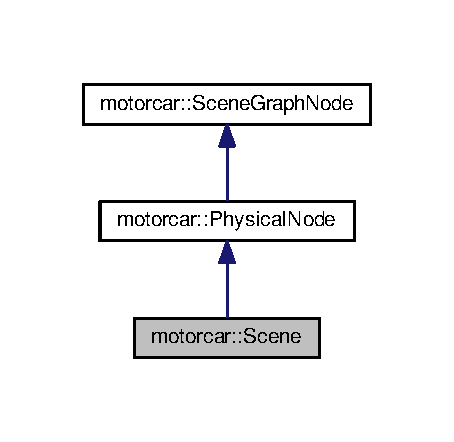
\includegraphics[height=550pt]{classmotorcar_1_1Scene__inherit__graph}
\end{center}
\end{figure}


Collaboration diagram for motorcar\-:\-:Scene\-:
\nopagebreak
\begin{figure}[H]
\begin{center}
\leavevmode
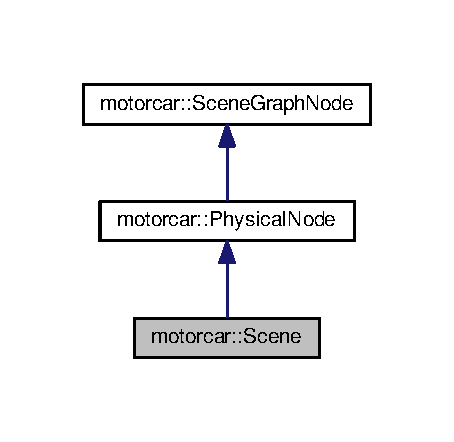
\includegraphics[height=550pt]{classmotorcar_1_1Scene__coll__graph}
\end{center}
\end{figure}
\subsection*{Public Member Functions}
\begin{DoxyCompactItemize}
\item 
\hyperlink{classmotorcar_1_1Scene_ad10176d75a9cc0da56626f682d083507}{Scene} ()
\item 
virtual \hyperlink{classmotorcar_1_1Scene_a07ad90930bf4792b88c8ce8b6800df4d}{$\sim$\-Scene} ()
\item 
virtual void \hyperlink{classmotorcar_1_1Scene_a11f9f856df5db6db78760cae5dc02079}{notify\-Node\-Added} (\hyperlink{classmotorcar_1_1SceneGraphNode}{Scene\-Graph\-Node} $\ast$node)
\item 
void \hyperlink{classmotorcar_1_1Scene_a3482161400b2f552307cc70812b128a9}{add\-Display} (\hyperlink{classmotorcar_1_1Display}{Display} $\ast$display)
\item 
std\-::vector$<$ \hyperlink{classmotorcar_1_1Display}{Display} $\ast$ $>$ \hyperlink{classmotorcar_1_1Scene_a1c09a0e3e55f1dd870d5c3001890afa9}{displays} () const 
\item 
void \hyperlink{classmotorcar_1_1Scene_ae8c9484b131cf87e8b1ebca4500343ae}{draw} (long delta\-Millis)
\item 
\hyperlink{classmotorcar_1_1WaylandSurfaceNode}{Wayland\-Surface\-Node} $\ast$ \hyperlink{classmotorcar_1_1Scene_a124b886baea9b583feb477202c9038a2}{cursor\-Node} () const 
\item 
void \hyperlink{classmotorcar_1_1Scene_a76a501d972979ba633dd0e38b022ab9b}{set\-Cursor\-Node} (\hyperlink{classmotorcar_1_1WaylandSurfaceNode}{Wayland\-Surface\-Node} $\ast$\hyperlink{classmotorcar_1_1Scene_a124b886baea9b583feb477202c9038a2}{cursor\-Node})
\item 
glm\-::ivec2 \hyperlink{classmotorcar_1_1Scene_abdb097ab9a2927b447b2eee485d19d6e}{cursor\-Hotspot} () const 
\item 
void \hyperlink{classmotorcar_1_1Scene_aba832b6a205b06b9d266ee3302ff86f4}{set\-Cursor\-Hotspot} (const glm\-::ivec2 \&\hyperlink{classmotorcar_1_1Scene_abdb097ab9a2927b447b2eee485d19d6e}{cursor\-Hotspot})
\end{DoxyCompactItemize}
\subsection*{Additional Inherited Members}


\subsection{Constructor \& Destructor Documentation}
\hypertarget{classmotorcar_1_1Scene_ad10176d75a9cc0da56626f682d083507}{\index{motorcar\-::\-Scene@{motorcar\-::\-Scene}!Scene@{Scene}}
\index{Scene@{Scene}!motorcar::Scene@{motorcar\-::\-Scene}}
\subsubsection[{Scene}]{\setlength{\rightskip}{0pt plus 5cm}Scene\-::\-Scene (
\begin{DoxyParamCaption}
{}
\end{DoxyParamCaption}
)}}\label{classmotorcar_1_1Scene_ad10176d75a9cc0da56626f682d083507}
\hypertarget{classmotorcar_1_1Scene_a07ad90930bf4792b88c8ce8b6800df4d}{\index{motorcar\-::\-Scene@{motorcar\-::\-Scene}!$\sim$\-Scene@{$\sim$\-Scene}}
\index{$\sim$\-Scene@{$\sim$\-Scene}!motorcar::Scene@{motorcar\-::\-Scene}}
\subsubsection[{$\sim$\-Scene}]{\setlength{\rightskip}{0pt plus 5cm}virtual motorcar\-::\-Scene\-::$\sim$\-Scene (
\begin{DoxyParamCaption}
{}
\end{DoxyParamCaption}
)\hspace{0.3cm}{\ttfamily [inline]}, {\ttfamily [virtual]}}}\label{classmotorcar_1_1Scene_a07ad90930bf4792b88c8ce8b6800df4d}


\subsection{Member Function Documentation}
\hypertarget{classmotorcar_1_1Scene_a3482161400b2f552307cc70812b128a9}{\index{motorcar\-::\-Scene@{motorcar\-::\-Scene}!add\-Display@{add\-Display}}
\index{add\-Display@{add\-Display}!motorcar::Scene@{motorcar\-::\-Scene}}
\subsubsection[{add\-Display}]{\setlength{\rightskip}{0pt plus 5cm}void Scene\-::add\-Display (
\begin{DoxyParamCaption}
\item[{{\bf Display} $\ast$}]{display}
\end{DoxyParamCaption}
)}}\label{classmotorcar_1_1Scene_a3482161400b2f552307cc70812b128a9}
\hypertarget{classmotorcar_1_1Scene_abdb097ab9a2927b447b2eee485d19d6e}{\index{motorcar\-::\-Scene@{motorcar\-::\-Scene}!cursor\-Hotspot@{cursor\-Hotspot}}
\index{cursor\-Hotspot@{cursor\-Hotspot}!motorcar::Scene@{motorcar\-::\-Scene}}
\subsubsection[{cursor\-Hotspot}]{\setlength{\rightskip}{0pt plus 5cm}glm\-::ivec2 Scene\-::cursor\-Hotspot (
\begin{DoxyParamCaption}
{}
\end{DoxyParamCaption}
) const}}\label{classmotorcar_1_1Scene_abdb097ab9a2927b447b2eee485d19d6e}
\hypertarget{classmotorcar_1_1Scene_a124b886baea9b583feb477202c9038a2}{\index{motorcar\-::\-Scene@{motorcar\-::\-Scene}!cursor\-Node@{cursor\-Node}}
\index{cursor\-Node@{cursor\-Node}!motorcar::Scene@{motorcar\-::\-Scene}}
\subsubsection[{cursor\-Node}]{\setlength{\rightskip}{0pt plus 5cm}{\bf Wayland\-Surface\-Node} $\ast$ Scene\-::cursor\-Node (
\begin{DoxyParamCaption}
{}
\end{DoxyParamCaption}
) const}}\label{classmotorcar_1_1Scene_a124b886baea9b583feb477202c9038a2}
\hypertarget{classmotorcar_1_1Scene_a1c09a0e3e55f1dd870d5c3001890afa9}{\index{motorcar\-::\-Scene@{motorcar\-::\-Scene}!displays@{displays}}
\index{displays@{displays}!motorcar::Scene@{motorcar\-::\-Scene}}
\subsubsection[{displays}]{\setlength{\rightskip}{0pt plus 5cm}std\-::vector$<$ {\bf Display} $\ast$ $>$ Scene\-::displays (
\begin{DoxyParamCaption}
{}
\end{DoxyParamCaption}
) const}}\label{classmotorcar_1_1Scene_a1c09a0e3e55f1dd870d5c3001890afa9}
\hypertarget{classmotorcar_1_1Scene_ae8c9484b131cf87e8b1ebca4500343ae}{\index{motorcar\-::\-Scene@{motorcar\-::\-Scene}!draw@{draw}}
\index{draw@{draw}!motorcar::Scene@{motorcar\-::\-Scene}}
\subsubsection[{draw}]{\setlength{\rightskip}{0pt plus 5cm}void Scene\-::draw (
\begin{DoxyParamCaption}
\item[{long}]{delta\-Millis}
\end{DoxyParamCaption}
)}}\label{classmotorcar_1_1Scene_ae8c9484b131cf87e8b1ebca4500343ae}
\hypertarget{classmotorcar_1_1Scene_a11f9f856df5db6db78760cae5dc02079}{\index{motorcar\-::\-Scene@{motorcar\-::\-Scene}!notify\-Node\-Added@{notify\-Node\-Added}}
\index{notify\-Node\-Added@{notify\-Node\-Added}!motorcar::Scene@{motorcar\-::\-Scene}}
\subsubsection[{notify\-Node\-Added}]{\setlength{\rightskip}{0pt plus 5cm}void Scene\-::notify\-Node\-Added (
\begin{DoxyParamCaption}
\item[{{\bf Scene\-Graph\-Node} $\ast$}]{node}
\end{DoxyParamCaption}
)\hspace{0.3cm}{\ttfamily [virtual]}}}\label{classmotorcar_1_1Scene_a11f9f856df5db6db78760cae5dc02079}
\hypertarget{classmotorcar_1_1Scene_aba832b6a205b06b9d266ee3302ff86f4}{\index{motorcar\-::\-Scene@{motorcar\-::\-Scene}!set\-Cursor\-Hotspot@{set\-Cursor\-Hotspot}}
\index{set\-Cursor\-Hotspot@{set\-Cursor\-Hotspot}!motorcar::Scene@{motorcar\-::\-Scene}}
\subsubsection[{set\-Cursor\-Hotspot}]{\setlength{\rightskip}{0pt plus 5cm}void Scene\-::set\-Cursor\-Hotspot (
\begin{DoxyParamCaption}
\item[{const glm\-::ivec2 \&}]{cursor\-Hotspot}
\end{DoxyParamCaption}
)}}\label{classmotorcar_1_1Scene_aba832b6a205b06b9d266ee3302ff86f4}
\hypertarget{classmotorcar_1_1Scene_a76a501d972979ba633dd0e38b022ab9b}{\index{motorcar\-::\-Scene@{motorcar\-::\-Scene}!set\-Cursor\-Node@{set\-Cursor\-Node}}
\index{set\-Cursor\-Node@{set\-Cursor\-Node}!motorcar::Scene@{motorcar\-::\-Scene}}
\subsubsection[{set\-Cursor\-Node}]{\setlength{\rightskip}{0pt plus 5cm}void Scene\-::set\-Cursor\-Node (
\begin{DoxyParamCaption}
\item[{{\bf Wayland\-Surface\-Node} $\ast$}]{cursor\-Node}
\end{DoxyParamCaption}
)}}\label{classmotorcar_1_1Scene_a76a501d972979ba633dd0e38b022ab9b}


The documentation for this class was generated from the following files\-:\begin{DoxyCompactItemize}
\item 
/home/dave/thesis/qtwayland-\/motorcar-\/compositor/motorcar/src/scenegraph/\hyperlink{scene_8h}{scene.\-h}\item 
/home/dave/thesis/qtwayland-\/motorcar-\/compositor/motorcar/src/scenegraph/\hyperlink{scene_8cpp}{scene.\-cpp}\end{DoxyCompactItemize}

\hypertarget{classmotorcar_1_1SceneGraphNode}{\section{motorcar\-:\-:Scene\-Graph\-Node Class Reference}
\label{classmotorcar_1_1SceneGraphNode}\index{motorcar\-::\-Scene\-Graph\-Node@{motorcar\-::\-Scene\-Graph\-Node}}
}


{\ttfamily \#include $<$scenegraphnode.\-h$>$}



Inheritance diagram for motorcar\-:\-:Scene\-Graph\-Node\-:
\nopagebreak
\begin{figure}[H]
\begin{center}
\leavevmode
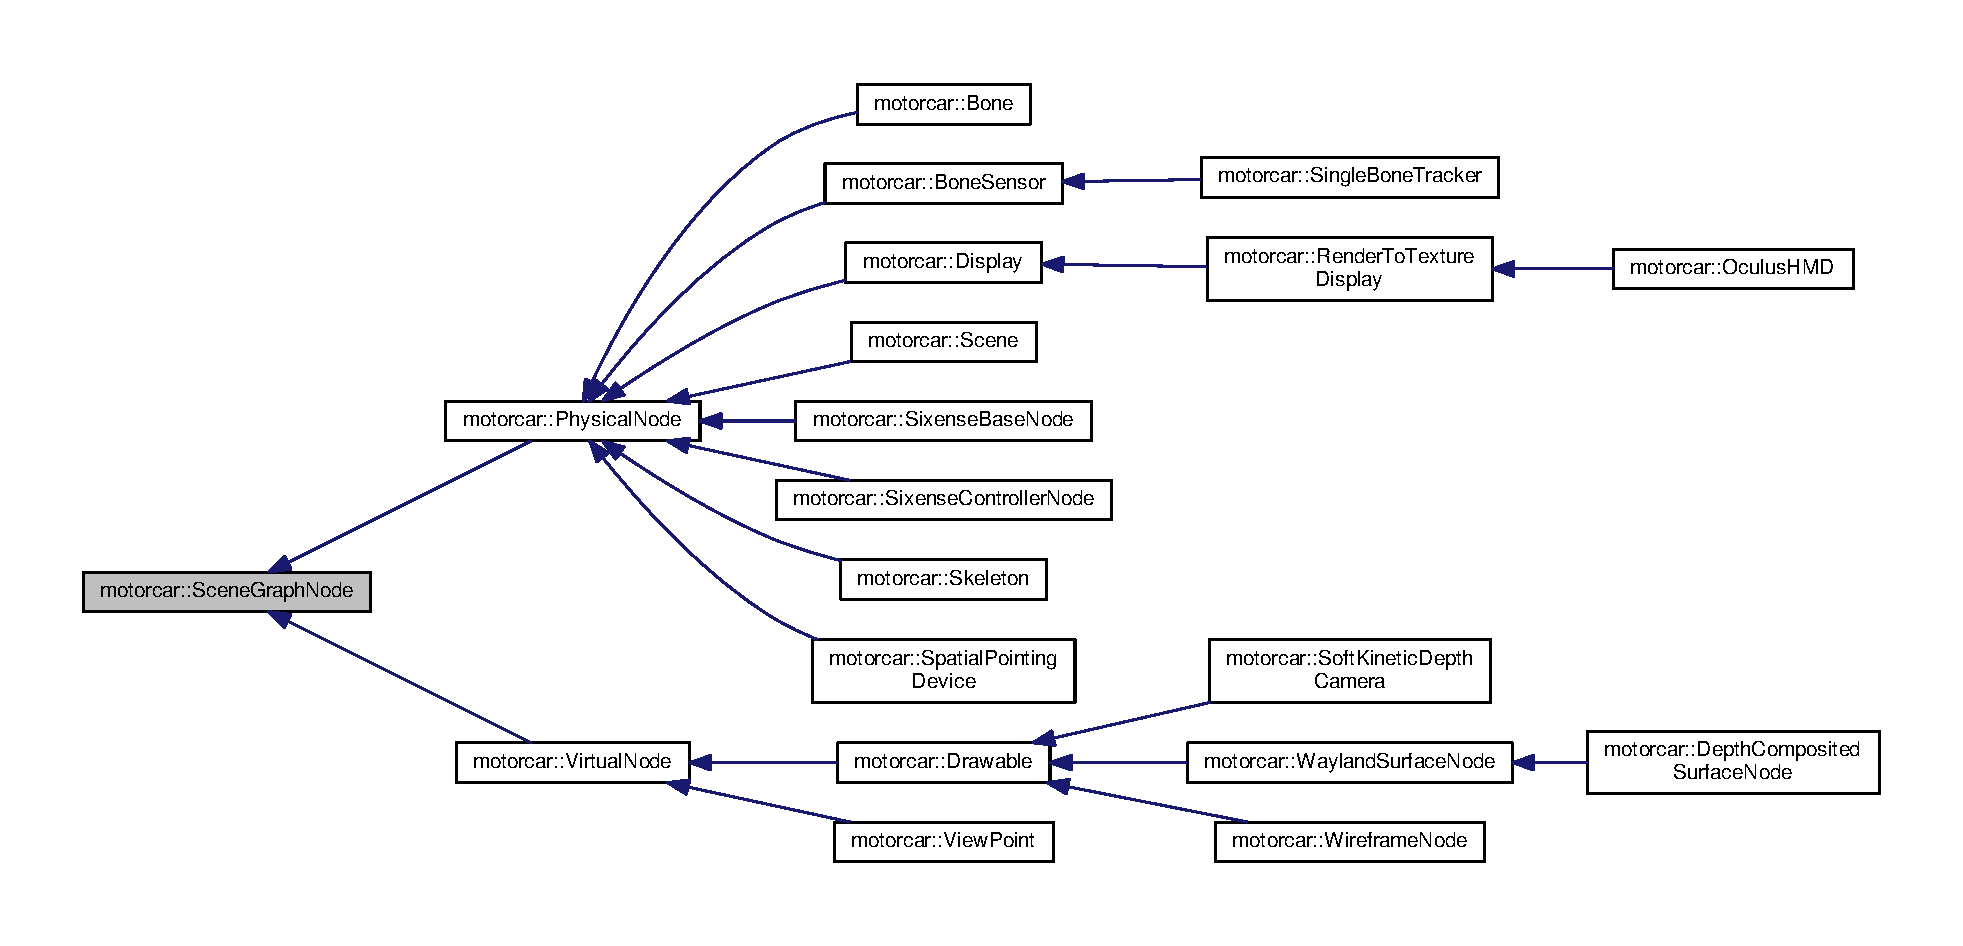
\includegraphics[width=350pt]{classmotorcar_1_1SceneGraphNode__inherit__graph}
\end{center}
\end{figure}


Collaboration diagram for motorcar\-:\-:Scene\-Graph\-Node\-:
\nopagebreak
\begin{figure}[H]
\begin{center}
\leavevmode
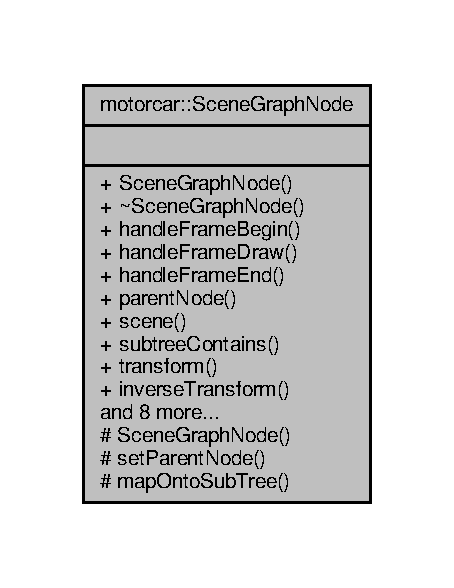
\includegraphics[width=218pt]{classmotorcar_1_1SceneGraphNode__coll__graph}
\end{center}
\end{figure}
\subsection*{Public Member Functions}
\begin{DoxyCompactItemize}
\item 
\hyperlink{classmotorcar_1_1SceneGraphNode_a293d96c3691afbaaba0da114a5e8f433}{Scene\-Graph\-Node} (\hyperlink{classmotorcar_1_1SceneGraphNode}{Scene\-Graph\-Node} $\ast$parent, glm\-::mat4 \hyperlink{classmotorcar_1_1SceneGraphNode_ad96e79fdd739ac8223a3128003be391a}{transform}=glm\-::mat4())
\item 
virtual \hyperlink{classmotorcar_1_1SceneGraphNode_ae81a28adc17e6be945c8279e4af4108c}{$\sim$\-Scene\-Graph\-Node} ()
\item 
virtual void \hyperlink{classmotorcar_1_1SceneGraphNode_aa680a8e89fc8ebd12b784653fb30c29a}{traverse\-Node} (\hyperlink{classmotorcar_1_1Scene}{Scene} $\ast$\hyperlink{classmotorcar_1_1SceneGraphNode_aa14e637ed4ae98f77e28941a4b5cfdd8}{scene}, long delta\-Millis)
\item 
void \hyperlink{classmotorcar_1_1SceneGraphNode_ac1e4d2185a8df5b84af1693a5d72d4fc}{traverse\-Scene\-Graph} (\hyperlink{classmotorcar_1_1Scene}{Scene} $\ast$\hyperlink{classmotorcar_1_1SceneGraphNode_aa14e637ed4ae98f77e28941a4b5cfdd8}{scene}, long delta\-Millis)
\item 
\hyperlink{classmotorcar_1_1SceneGraphNode}{Scene\-Graph\-Node} $\ast$ \hyperlink{classmotorcar_1_1SceneGraphNode_a57dd5826ed6bf15c8a879f5a090c6000}{parent\-Node} () const 
\item 
\hyperlink{classmotorcar_1_1Scene}{Scene} $\ast$ \hyperlink{classmotorcar_1_1SceneGraphNode_aa14e637ed4ae98f77e28941a4b5cfdd8}{scene} ()
\item 
bool \hyperlink{classmotorcar_1_1SceneGraphNode_ac2be631270bc40cb1e070983c30a323f}{subtree\-Contains} (\hyperlink{classmotorcar_1_1SceneGraphNode}{Scene\-Graph\-Node} $\ast$node)
\item 
glm\-::mat4 \hyperlink{classmotorcar_1_1SceneGraphNode_ad96e79fdd739ac8223a3128003be391a}{transform} () const 
\item 
glm\-::mat4 \hyperlink{classmotorcar_1_1SceneGraphNode_af8b8174098f1de1067541f0e3ebec72e}{inverse\-Transform} () const 
\item 
void \hyperlink{classmotorcar_1_1SceneGraphNode_a7cd7700336833efa89c8004e85a1fd61}{set\-Transform} (const glm\-::mat4 \&\hyperlink{classmotorcar_1_1SceneGraphNode_ad96e79fdd739ac8223a3128003be391a}{transform})
\item 
glm\-::mat4 \hyperlink{classmotorcar_1_1SceneGraphNode_a3e7fba2add3f63a65f31996f0ce9c9bf}{world\-Transform} () const 
\item 
glm\-::mat4 \hyperlink{classmotorcar_1_1SceneGraphNode_a10e4fd743e891cef676435c5f5d5467d}{inverse\-World\-Transform} () const 
\item 
void \hyperlink{classmotorcar_1_1SceneGraphNode_ac1a30cbe4af18133b19e6f852c33e30a}{set\-World\-Transform} (const glm\-::mat4 \&\hyperlink{classmotorcar_1_1SceneGraphNode_ad96e79fdd739ac8223a3128003be391a}{transform})
\item 
virtual \\*
\hyperlink{structmotorcar_1_1Geometry_1_1RaySurfaceIntersection}{Geometry\-::\-Ray\-Surface\-Intersection} $\ast$ \hyperlink{classmotorcar_1_1SceneGraphNode_ac268b171317430368fcc7733eab05ae6}{intersect\-With\-Surfaces} (const \hyperlink{structmotorcar_1_1Geometry_1_1Ray}{Geometry\-::\-Ray} \&ray)
\item 
std\-::vector$<$ \hyperlink{classmotorcar_1_1SceneGraphNode}{Scene\-Graph\-Node} $\ast$ $>$ \hyperlink{classmotorcar_1_1SceneGraphNode_a9a0c649390da0918afd58805192ccdca}{child\-Nodes} () const 
\item 
std\-::vector$<$ \hyperlink{classmotorcar_1_1SceneGraphNode}{Scene\-Graph\-Node} $\ast$ $>$ \hyperlink{classmotorcar_1_1SceneGraphNode_aa7ac1c085afbe0fb0b9d5cd578a8c4ef}{nodes\-In\-Subtree} () const 
\end{DoxyCompactItemize}
\subsection*{Protected Member Functions}
\begin{DoxyCompactItemize}
\item 
\hyperlink{classmotorcar_1_1SceneGraphNode_ab9bc5f59ccba332aab918c7b066c309f}{Scene\-Graph\-Node} ()
\item 
void \hyperlink{classmotorcar_1_1SceneGraphNode_a977b156ebcc07018a475b4042de8886a}{set\-Parent\-Node} (\hyperlink{classmotorcar_1_1SceneGraphNode}{Scene\-Graph\-Node} $\ast$parent)
\end{DoxyCompactItemize}


\subsection{Constructor \& Destructor Documentation}
\hypertarget{classmotorcar_1_1SceneGraphNode_a293d96c3691afbaaba0da114a5e8f433}{\index{motorcar\-::\-Scene\-Graph\-Node@{motorcar\-::\-Scene\-Graph\-Node}!Scene\-Graph\-Node@{Scene\-Graph\-Node}}
\index{Scene\-Graph\-Node@{Scene\-Graph\-Node}!motorcar::SceneGraphNode@{motorcar\-::\-Scene\-Graph\-Node}}
\subsubsection[{Scene\-Graph\-Node}]{\setlength{\rightskip}{0pt plus 5cm}Scene\-Graph\-Node\-::\-Scene\-Graph\-Node (
\begin{DoxyParamCaption}
\item[{{\bf Scene\-Graph\-Node} $\ast$}]{parent, }
\item[{glm\-::mat4}]{transform = {\ttfamily glm\-:\-:mat4()}}
\end{DoxyParamCaption}
)}}\label{classmotorcar_1_1SceneGraphNode_a293d96c3691afbaaba0da114a5e8f433}
\hypertarget{classmotorcar_1_1SceneGraphNode_ae81a28adc17e6be945c8279e4af4108c}{\index{motorcar\-::\-Scene\-Graph\-Node@{motorcar\-::\-Scene\-Graph\-Node}!$\sim$\-Scene\-Graph\-Node@{$\sim$\-Scene\-Graph\-Node}}
\index{$\sim$\-Scene\-Graph\-Node@{$\sim$\-Scene\-Graph\-Node}!motorcar::SceneGraphNode@{motorcar\-::\-Scene\-Graph\-Node}}
\subsubsection[{$\sim$\-Scene\-Graph\-Node}]{\setlength{\rightskip}{0pt plus 5cm}Scene\-Graph\-Node\-::$\sim$\-Scene\-Graph\-Node (
\begin{DoxyParamCaption}
{}
\end{DoxyParamCaption}
)\hspace{0.3cm}{\ttfamily [virtual]}}}\label{classmotorcar_1_1SceneGraphNode_ae81a28adc17e6be945c8279e4af4108c}
\hypertarget{classmotorcar_1_1SceneGraphNode_ab9bc5f59ccba332aab918c7b066c309f}{\index{motorcar\-::\-Scene\-Graph\-Node@{motorcar\-::\-Scene\-Graph\-Node}!Scene\-Graph\-Node@{Scene\-Graph\-Node}}
\index{Scene\-Graph\-Node@{Scene\-Graph\-Node}!motorcar::SceneGraphNode@{motorcar\-::\-Scene\-Graph\-Node}}
\subsubsection[{Scene\-Graph\-Node}]{\setlength{\rightskip}{0pt plus 5cm}Scene\-Graph\-Node\-::\-Scene\-Graph\-Node (
\begin{DoxyParamCaption}
{}
\end{DoxyParamCaption}
)\hspace{0.3cm}{\ttfamily [protected]}}}\label{classmotorcar_1_1SceneGraphNode_ab9bc5f59ccba332aab918c7b066c309f}


\subsection{Member Function Documentation}
\hypertarget{classmotorcar_1_1SceneGraphNode_a9a0c649390da0918afd58805192ccdca}{\index{motorcar\-::\-Scene\-Graph\-Node@{motorcar\-::\-Scene\-Graph\-Node}!child\-Nodes@{child\-Nodes}}
\index{child\-Nodes@{child\-Nodes}!motorcar::SceneGraphNode@{motorcar\-::\-Scene\-Graph\-Node}}
\subsubsection[{child\-Nodes}]{\setlength{\rightskip}{0pt plus 5cm}std\-::vector$<$ {\bf Scene\-Graph\-Node} $\ast$ $>$ Scene\-Graph\-Node\-::child\-Nodes (
\begin{DoxyParamCaption}
{}
\end{DoxyParamCaption}
) const}}\label{classmotorcar_1_1SceneGraphNode_a9a0c649390da0918afd58805192ccdca}
\hypertarget{classmotorcar_1_1SceneGraphNode_ac268b171317430368fcc7733eab05ae6}{\index{motorcar\-::\-Scene\-Graph\-Node@{motorcar\-::\-Scene\-Graph\-Node}!intersect\-With\-Surfaces@{intersect\-With\-Surfaces}}
\index{intersect\-With\-Surfaces@{intersect\-With\-Surfaces}!motorcar::SceneGraphNode@{motorcar\-::\-Scene\-Graph\-Node}}
\subsubsection[{intersect\-With\-Surfaces}]{\setlength{\rightskip}{0pt plus 5cm}{\bf Geometry\-::\-Ray\-Surface\-Intersection} $\ast$ Scene\-Graph\-Node\-::intersect\-With\-Surfaces (
\begin{DoxyParamCaption}
\item[{const {\bf Geometry\-::\-Ray} \&}]{ray}
\end{DoxyParamCaption}
)\hspace{0.3cm}{\ttfamily [virtual]}}}\label{classmotorcar_1_1SceneGraphNode_ac268b171317430368fcc7733eab05ae6}


Reimplemented in \hyperlink{classmotorcar_1_1WaylandSurfaceNode_adf71a714d07bb262405a361504a77ea4}{motorcar\-::\-Wayland\-Surface\-Node}.

\hypertarget{classmotorcar_1_1SceneGraphNode_af8b8174098f1de1067541f0e3ebec72e}{\index{motorcar\-::\-Scene\-Graph\-Node@{motorcar\-::\-Scene\-Graph\-Node}!inverse\-Transform@{inverse\-Transform}}
\index{inverse\-Transform@{inverse\-Transform}!motorcar::SceneGraphNode@{motorcar\-::\-Scene\-Graph\-Node}}
\subsubsection[{inverse\-Transform}]{\setlength{\rightskip}{0pt plus 5cm}glm\-::mat4 Scene\-Graph\-Node\-::inverse\-Transform (
\begin{DoxyParamCaption}
{}
\end{DoxyParamCaption}
) const}}\label{classmotorcar_1_1SceneGraphNode_af8b8174098f1de1067541f0e3ebec72e}
\hypertarget{classmotorcar_1_1SceneGraphNode_a10e4fd743e891cef676435c5f5d5467d}{\index{motorcar\-::\-Scene\-Graph\-Node@{motorcar\-::\-Scene\-Graph\-Node}!inverse\-World\-Transform@{inverse\-World\-Transform}}
\index{inverse\-World\-Transform@{inverse\-World\-Transform}!motorcar::SceneGraphNode@{motorcar\-::\-Scene\-Graph\-Node}}
\subsubsection[{inverse\-World\-Transform}]{\setlength{\rightskip}{0pt plus 5cm}glm\-::mat4 Scene\-Graph\-Node\-::inverse\-World\-Transform (
\begin{DoxyParamCaption}
{}
\end{DoxyParamCaption}
) const}}\label{classmotorcar_1_1SceneGraphNode_a10e4fd743e891cef676435c5f5d5467d}
\hypertarget{classmotorcar_1_1SceneGraphNode_aa7ac1c085afbe0fb0b9d5cd578a8c4ef}{\index{motorcar\-::\-Scene\-Graph\-Node@{motorcar\-::\-Scene\-Graph\-Node}!nodes\-In\-Subtree@{nodes\-In\-Subtree}}
\index{nodes\-In\-Subtree@{nodes\-In\-Subtree}!motorcar::SceneGraphNode@{motorcar\-::\-Scene\-Graph\-Node}}
\subsubsection[{nodes\-In\-Subtree}]{\setlength{\rightskip}{0pt plus 5cm}std\-::vector$<$ {\bf Scene\-Graph\-Node} $\ast$ $>$ Scene\-Graph\-Node\-::nodes\-In\-Subtree (
\begin{DoxyParamCaption}
{}
\end{DoxyParamCaption}
) const}}\label{classmotorcar_1_1SceneGraphNode_aa7ac1c085afbe0fb0b9d5cd578a8c4ef}
\hypertarget{classmotorcar_1_1SceneGraphNode_a57dd5826ed6bf15c8a879f5a090c6000}{\index{motorcar\-::\-Scene\-Graph\-Node@{motorcar\-::\-Scene\-Graph\-Node}!parent\-Node@{parent\-Node}}
\index{parent\-Node@{parent\-Node}!motorcar::SceneGraphNode@{motorcar\-::\-Scene\-Graph\-Node}}
\subsubsection[{parent\-Node}]{\setlength{\rightskip}{0pt plus 5cm}{\bf Scene\-Graph\-Node} $\ast$ Scene\-Graph\-Node\-::parent\-Node (
\begin{DoxyParamCaption}
{}
\end{DoxyParamCaption}
) const}}\label{classmotorcar_1_1SceneGraphNode_a57dd5826ed6bf15c8a879f5a090c6000}
\hypertarget{classmotorcar_1_1SceneGraphNode_aa14e637ed4ae98f77e28941a4b5cfdd8}{\index{motorcar\-::\-Scene\-Graph\-Node@{motorcar\-::\-Scene\-Graph\-Node}!scene@{scene}}
\index{scene@{scene}!motorcar::SceneGraphNode@{motorcar\-::\-Scene\-Graph\-Node}}
\subsubsection[{scene}]{\setlength{\rightskip}{0pt plus 5cm}{\bf Scene} $\ast$ Scene\-Graph\-Node\-::scene (
\begin{DoxyParamCaption}
{}
\end{DoxyParamCaption}
)}}\label{classmotorcar_1_1SceneGraphNode_aa14e637ed4ae98f77e28941a4b5cfdd8}
\hypertarget{classmotorcar_1_1SceneGraphNode_a977b156ebcc07018a475b4042de8886a}{\index{motorcar\-::\-Scene\-Graph\-Node@{motorcar\-::\-Scene\-Graph\-Node}!set\-Parent\-Node@{set\-Parent\-Node}}
\index{set\-Parent\-Node@{set\-Parent\-Node}!motorcar::SceneGraphNode@{motorcar\-::\-Scene\-Graph\-Node}}
\subsubsection[{set\-Parent\-Node}]{\setlength{\rightskip}{0pt plus 5cm}void Scene\-Graph\-Node\-::set\-Parent\-Node (
\begin{DoxyParamCaption}
\item[{{\bf Scene\-Graph\-Node} $\ast$}]{parent}
\end{DoxyParamCaption}
)\hspace{0.3cm}{\ttfamily [protected]}}}\label{classmotorcar_1_1SceneGraphNode_a977b156ebcc07018a475b4042de8886a}
\hypertarget{classmotorcar_1_1SceneGraphNode_a7cd7700336833efa89c8004e85a1fd61}{\index{motorcar\-::\-Scene\-Graph\-Node@{motorcar\-::\-Scene\-Graph\-Node}!set\-Transform@{set\-Transform}}
\index{set\-Transform@{set\-Transform}!motorcar::SceneGraphNode@{motorcar\-::\-Scene\-Graph\-Node}}
\subsubsection[{set\-Transform}]{\setlength{\rightskip}{0pt plus 5cm}void Scene\-Graph\-Node\-::set\-Transform (
\begin{DoxyParamCaption}
\item[{const glm\-::mat4 \&}]{transform}
\end{DoxyParamCaption}
)}}\label{classmotorcar_1_1SceneGraphNode_a7cd7700336833efa89c8004e85a1fd61}
\hypertarget{classmotorcar_1_1SceneGraphNode_ac1a30cbe4af18133b19e6f852c33e30a}{\index{motorcar\-::\-Scene\-Graph\-Node@{motorcar\-::\-Scene\-Graph\-Node}!set\-World\-Transform@{set\-World\-Transform}}
\index{set\-World\-Transform@{set\-World\-Transform}!motorcar::SceneGraphNode@{motorcar\-::\-Scene\-Graph\-Node}}
\subsubsection[{set\-World\-Transform}]{\setlength{\rightskip}{0pt plus 5cm}void Scene\-Graph\-Node\-::set\-World\-Transform (
\begin{DoxyParamCaption}
\item[{const glm\-::mat4 \&}]{transform}
\end{DoxyParamCaption}
)}}\label{classmotorcar_1_1SceneGraphNode_ac1a30cbe4af18133b19e6f852c33e30a}
\hypertarget{classmotorcar_1_1SceneGraphNode_ac2be631270bc40cb1e070983c30a323f}{\index{motorcar\-::\-Scene\-Graph\-Node@{motorcar\-::\-Scene\-Graph\-Node}!subtree\-Contains@{subtree\-Contains}}
\index{subtree\-Contains@{subtree\-Contains}!motorcar::SceneGraphNode@{motorcar\-::\-Scene\-Graph\-Node}}
\subsubsection[{subtree\-Contains}]{\setlength{\rightskip}{0pt plus 5cm}bool Scene\-Graph\-Node\-::subtree\-Contains (
\begin{DoxyParamCaption}
\item[{{\bf Scene\-Graph\-Node} $\ast$}]{node}
\end{DoxyParamCaption}
)}}\label{classmotorcar_1_1SceneGraphNode_ac2be631270bc40cb1e070983c30a323f}
\hypertarget{classmotorcar_1_1SceneGraphNode_ad96e79fdd739ac8223a3128003be391a}{\index{motorcar\-::\-Scene\-Graph\-Node@{motorcar\-::\-Scene\-Graph\-Node}!transform@{transform}}
\index{transform@{transform}!motorcar::SceneGraphNode@{motorcar\-::\-Scene\-Graph\-Node}}
\subsubsection[{transform}]{\setlength{\rightskip}{0pt plus 5cm}glm\-::mat4 Scene\-Graph\-Node\-::transform (
\begin{DoxyParamCaption}
{}
\end{DoxyParamCaption}
) const}}\label{classmotorcar_1_1SceneGraphNode_ad96e79fdd739ac8223a3128003be391a}
\hypertarget{classmotorcar_1_1SceneGraphNode_aa680a8e89fc8ebd12b784653fb30c29a}{\index{motorcar\-::\-Scene\-Graph\-Node@{motorcar\-::\-Scene\-Graph\-Node}!traverse\-Node@{traverse\-Node}}
\index{traverse\-Node@{traverse\-Node}!motorcar::SceneGraphNode@{motorcar\-::\-Scene\-Graph\-Node}}
\subsubsection[{traverse\-Node}]{\setlength{\rightskip}{0pt plus 5cm}void Scene\-Graph\-Node\-::traverse\-Node (
\begin{DoxyParamCaption}
\item[{{\bf Scene} $\ast$}]{scene, }
\item[{long}]{delta\-Millis}
\end{DoxyParamCaption}
)\hspace{0.3cm}{\ttfamily [virtual]}}}\label{classmotorcar_1_1SceneGraphNode_aa680a8e89fc8ebd12b784653fb30c29a}


Reimplemented in \hyperlink{classmotorcar_1_1SixenseControllerNode_ab525f98319a51aff7043b79dc137e26f}{motorcar\-::\-Sixense\-Controller\-Node}, \hyperlink{classmotorcar_1_1SpatialPointingDevice_a53e251f5a0d7a9b0b8e7dc84d2e9d078}{motorcar\-::\-Spatial\-Pointing\-Device}, \hyperlink{classmotorcar_1_1VirtualNode_ad0eda301331d02d5bf03d13432e62d17}{motorcar\-::\-Virtual\-Node}, \hyperlink{classmotorcar_1_1Drawable_a931cb72d30d280d0e63f22c2e1ac39c6}{motorcar\-::\-Drawable}, and \hyperlink{classmotorcar_1_1SixenseBaseNode_a6454bbe79106600cdd7b92c2f30f7f63}{motorcar\-::\-Sixense\-Base\-Node}.

\hypertarget{classmotorcar_1_1SceneGraphNode_ac1e4d2185a8df5b84af1693a5d72d4fc}{\index{motorcar\-::\-Scene\-Graph\-Node@{motorcar\-::\-Scene\-Graph\-Node}!traverse\-Scene\-Graph@{traverse\-Scene\-Graph}}
\index{traverse\-Scene\-Graph@{traverse\-Scene\-Graph}!motorcar::SceneGraphNode@{motorcar\-::\-Scene\-Graph\-Node}}
\subsubsection[{traverse\-Scene\-Graph}]{\setlength{\rightskip}{0pt plus 5cm}void Scene\-Graph\-Node\-::traverse\-Scene\-Graph (
\begin{DoxyParamCaption}
\item[{{\bf Scene} $\ast$}]{scene, }
\item[{long}]{delta\-Millis}
\end{DoxyParamCaption}
)}}\label{classmotorcar_1_1SceneGraphNode_ac1e4d2185a8df5b84af1693a5d72d4fc}
\hypertarget{classmotorcar_1_1SceneGraphNode_a3e7fba2add3f63a65f31996f0ce9c9bf}{\index{motorcar\-::\-Scene\-Graph\-Node@{motorcar\-::\-Scene\-Graph\-Node}!world\-Transform@{world\-Transform}}
\index{world\-Transform@{world\-Transform}!motorcar::SceneGraphNode@{motorcar\-::\-Scene\-Graph\-Node}}
\subsubsection[{world\-Transform}]{\setlength{\rightskip}{0pt plus 5cm}glm\-::mat4 Scene\-Graph\-Node\-::world\-Transform (
\begin{DoxyParamCaption}
{}
\end{DoxyParamCaption}
) const}}\label{classmotorcar_1_1SceneGraphNode_a3e7fba2add3f63a65f31996f0ce9c9bf}


The documentation for this class was generated from the following files\-:\begin{DoxyCompactItemize}
\item 
/home/dave/thesis/qtwayland-\/motorcar-\/compositor/motorcar/src/scenegraph/\hyperlink{scenegraphnode_8h}{scenegraphnode.\-h}\item 
/home/dave/thesis/qtwayland-\/motorcar-\/compositor/motorcar/src/scenegraph/\hyperlink{scenegraphnode_8cpp}{scenegraphnode.\-cpp}\end{DoxyCompactItemize}

\hypertarget{classmotorcar_1_1Seat}{\section{motorcar\-:\-:Seat Class Reference}
\label{classmotorcar_1_1Seat}\index{motorcar\-::\-Seat@{motorcar\-::\-Seat}}
}


{\ttfamily \#include $<$seat.\-h$>$}



Inheritance diagram for motorcar\-:\-:Seat\-:
\nopagebreak
\begin{figure}[H]
\begin{center}
\leavevmode
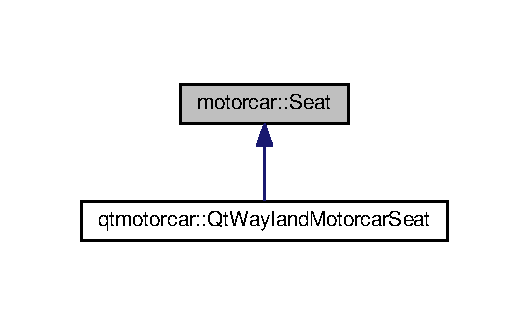
\includegraphics[width=254pt]{classmotorcar_1_1Seat__inherit__graph}
\end{center}
\end{figure}
\subsection*{Public Member Functions}
\begin{DoxyCompactItemize}
\item 
\hyperlink{classmotorcar_1_1Seat_a7fbd40f66e504cd214797c95dd83c94c}{Seat} ()
\item 
virtual \hyperlink{classmotorcar_1_1Seat_a28ee91e80c53d92b8729adf9248dca97}{$\sim$\-Seat} ()
\item 
\hyperlink{classmotorcar_1_1Keyboard}{Keyboard} $\ast$ \hyperlink{classmotorcar_1_1Seat_ada346c548a070764bd05b7666b04ba28}{keyboard} () const 
\item 
void \hyperlink{classmotorcar_1_1Seat_ac73c8ea32eaffeccbed3fdfe4d115428}{set\-Keyboard} (\hyperlink{classmotorcar_1_1Keyboard}{Keyboard} $\ast$\hyperlink{classmotorcar_1_1Seat_ada346c548a070764bd05b7666b04ba28}{keyboard})
\item 
\hyperlink{classmotorcar_1_1WaylandSurface}{Wayland\-Surface} $\ast$ \hyperlink{classmotorcar_1_1Seat_a4ac963bf0d54b6e4a77c0594b37d756f}{keyboard\-Focus} () const 
\item 
virtual void \hyperlink{classmotorcar_1_1Seat_ab8f8eb12135b5db96238c37653fb54d1}{set\-Keyboard\-Focus} (\hyperlink{classmotorcar_1_1WaylandSurface}{Wayland\-Surface} $\ast$\hyperlink{classmotorcar_1_1Seat_a4ac963bf0d54b6e4a77c0594b37d756f}{keyboard\-Focus})
\item 
\hyperlink{classmotorcar_1_1Pointer}{Pointer} $\ast$ \hyperlink{classmotorcar_1_1Seat_a98193b334b8a8278b29926f9f97300c6}{pointer} () const 
\item 
void \hyperlink{classmotorcar_1_1Seat_ae84831d0c43b89bbeb0ff7c1b0186c5d}{set\-Pointer} (\hyperlink{classmotorcar_1_1Pointer}{Pointer} $\ast$\hyperlink{classmotorcar_1_1Seat_a98193b334b8a8278b29926f9f97300c6}{pointer})
\item 
\hyperlink{classmotorcar_1_1WaylandSurface}{Wayland\-Surface} $\ast$ \hyperlink{classmotorcar_1_1Seat_a996631e534a7c9424245c03c1781fd2a}{pointer\-Focus} () const 
\item 
virtual void \hyperlink{classmotorcar_1_1Seat_a0f7254a717c97aba66b15ca8d437734c}{set\-Pointer\-Focus} (\hyperlink{classmotorcar_1_1WaylandSurface}{Wayland\-Surface} $\ast$\hyperlink{classmotorcar_1_1Seat_a996631e534a7c9424245c03c1781fd2a}{pointer\-Focus}, glm\-::vec2 local\-Position)
\item 
void \hyperlink{classmotorcar_1_1Seat_a40f9d76a799f70acd1cd3ad5f0360aad}{ensure\-Keyboard\-Focus\-Is\-Valid} (\hyperlink{classmotorcar_1_1WaylandSurface}{Wayland\-Surface} $\ast$old\-Surface, \hyperlink{classmotorcar_1_1WaylandSurface}{Wayland\-Surface} $\ast$next\-Surface)
\begin{DoxyCompactList}\small\item\em Guaruntees that the current keyboard focus is as valid possible. \end{DoxyCompactList}\end{DoxyCompactItemize}


\subsection{Constructor \& Destructor Documentation}
\hypertarget{classmotorcar_1_1Seat_a7fbd40f66e504cd214797c95dd83c94c}{\index{motorcar\-::\-Seat@{motorcar\-::\-Seat}!Seat@{Seat}}
\index{Seat@{Seat}!motorcar::Seat@{motorcar\-::\-Seat}}
\subsubsection[{Seat}]{\setlength{\rightskip}{0pt plus 5cm}Seat\-::\-Seat (
\begin{DoxyParamCaption}
{}
\end{DoxyParamCaption}
)}}\label{classmotorcar_1_1Seat_a7fbd40f66e504cd214797c95dd83c94c}
\hypertarget{classmotorcar_1_1Seat_a28ee91e80c53d92b8729adf9248dca97}{\index{motorcar\-::\-Seat@{motorcar\-::\-Seat}!$\sim$\-Seat@{$\sim$\-Seat}}
\index{$\sim$\-Seat@{$\sim$\-Seat}!motorcar::Seat@{motorcar\-::\-Seat}}
\subsubsection[{$\sim$\-Seat}]{\setlength{\rightskip}{0pt plus 5cm}Seat\-::$\sim$\-Seat (
\begin{DoxyParamCaption}
{}
\end{DoxyParamCaption}
)\hspace{0.3cm}{\ttfamily [virtual]}}}\label{classmotorcar_1_1Seat_a28ee91e80c53d92b8729adf9248dca97}


\subsection{Member Function Documentation}
\hypertarget{classmotorcar_1_1Seat_a40f9d76a799f70acd1cd3ad5f0360aad}{\index{motorcar\-::\-Seat@{motorcar\-::\-Seat}!ensure\-Keyboard\-Focus\-Is\-Valid@{ensure\-Keyboard\-Focus\-Is\-Valid}}
\index{ensure\-Keyboard\-Focus\-Is\-Valid@{ensure\-Keyboard\-Focus\-Is\-Valid}!motorcar::Seat@{motorcar\-::\-Seat}}
\subsubsection[{ensure\-Keyboard\-Focus\-Is\-Valid}]{\setlength{\rightskip}{0pt plus 5cm}void Seat\-::ensure\-Keyboard\-Focus\-Is\-Valid (
\begin{DoxyParamCaption}
\item[{{\bf Wayland\-Surface} $\ast$}]{old\-Surface, }
\item[{{\bf Wayland\-Surface} $\ast$}]{next\-Surface}
\end{DoxyParamCaption}
)}}\label{classmotorcar_1_1Seat_a40f9d76a799f70acd1cd3ad5f0360aad}


Guaruntees that the current keyboard focus is as valid possible. 

\hypertarget{classmotorcar_1_1Seat_ada346c548a070764bd05b7666b04ba28}{\index{motorcar\-::\-Seat@{motorcar\-::\-Seat}!keyboard@{keyboard}}
\index{keyboard@{keyboard}!motorcar::Seat@{motorcar\-::\-Seat}}
\subsubsection[{keyboard}]{\setlength{\rightskip}{0pt plus 5cm}{\bf Keyboard} $\ast$ Seat\-::keyboard (
\begin{DoxyParamCaption}
{}
\end{DoxyParamCaption}
) const}}\label{classmotorcar_1_1Seat_ada346c548a070764bd05b7666b04ba28}
\hypertarget{classmotorcar_1_1Seat_a4ac963bf0d54b6e4a77c0594b37d756f}{\index{motorcar\-::\-Seat@{motorcar\-::\-Seat}!keyboard\-Focus@{keyboard\-Focus}}
\index{keyboard\-Focus@{keyboard\-Focus}!motorcar::Seat@{motorcar\-::\-Seat}}
\subsubsection[{keyboard\-Focus}]{\setlength{\rightskip}{0pt plus 5cm}{\bf Wayland\-Surface} $\ast$ Seat\-::keyboard\-Focus (
\begin{DoxyParamCaption}
{}
\end{DoxyParamCaption}
) const}}\label{classmotorcar_1_1Seat_a4ac963bf0d54b6e4a77c0594b37d756f}
\hypertarget{classmotorcar_1_1Seat_a98193b334b8a8278b29926f9f97300c6}{\index{motorcar\-::\-Seat@{motorcar\-::\-Seat}!pointer@{pointer}}
\index{pointer@{pointer}!motorcar::Seat@{motorcar\-::\-Seat}}
\subsubsection[{pointer}]{\setlength{\rightskip}{0pt plus 5cm}{\bf Pointer} $\ast$ Seat\-::pointer (
\begin{DoxyParamCaption}
{}
\end{DoxyParamCaption}
) const}}\label{classmotorcar_1_1Seat_a98193b334b8a8278b29926f9f97300c6}
\hypertarget{classmotorcar_1_1Seat_a996631e534a7c9424245c03c1781fd2a}{\index{motorcar\-::\-Seat@{motorcar\-::\-Seat}!pointer\-Focus@{pointer\-Focus}}
\index{pointer\-Focus@{pointer\-Focus}!motorcar::Seat@{motorcar\-::\-Seat}}
\subsubsection[{pointer\-Focus}]{\setlength{\rightskip}{0pt plus 5cm}{\bf Wayland\-Surface} $\ast$ Seat\-::pointer\-Focus (
\begin{DoxyParamCaption}
{}
\end{DoxyParamCaption}
) const}}\label{classmotorcar_1_1Seat_a996631e534a7c9424245c03c1781fd2a}
\hypertarget{classmotorcar_1_1Seat_ac73c8ea32eaffeccbed3fdfe4d115428}{\index{motorcar\-::\-Seat@{motorcar\-::\-Seat}!set\-Keyboard@{set\-Keyboard}}
\index{set\-Keyboard@{set\-Keyboard}!motorcar::Seat@{motorcar\-::\-Seat}}
\subsubsection[{set\-Keyboard}]{\setlength{\rightskip}{0pt plus 5cm}void Seat\-::set\-Keyboard (
\begin{DoxyParamCaption}
\item[{{\bf Keyboard} $\ast$}]{keyboard}
\end{DoxyParamCaption}
)}}\label{classmotorcar_1_1Seat_ac73c8ea32eaffeccbed3fdfe4d115428}
\hypertarget{classmotorcar_1_1Seat_ab8f8eb12135b5db96238c37653fb54d1}{\index{motorcar\-::\-Seat@{motorcar\-::\-Seat}!set\-Keyboard\-Focus@{set\-Keyboard\-Focus}}
\index{set\-Keyboard\-Focus@{set\-Keyboard\-Focus}!motorcar::Seat@{motorcar\-::\-Seat}}
\subsubsection[{set\-Keyboard\-Focus}]{\setlength{\rightskip}{0pt plus 5cm}void Seat\-::set\-Keyboard\-Focus (
\begin{DoxyParamCaption}
\item[{{\bf Wayland\-Surface} $\ast$}]{keyboard\-Focus}
\end{DoxyParamCaption}
)\hspace{0.3cm}{\ttfamily [virtual]}}}\label{classmotorcar_1_1Seat_ab8f8eb12135b5db96238c37653fb54d1}


Reimplemented in \hyperlink{classqtmotorcar_1_1QtWaylandMotorcarSeat_a28e6eb540028abe6d70ecd5b7320d6aa}{qtmotorcar\-::\-Qt\-Wayland\-Motorcar\-Seat}.

\hypertarget{classmotorcar_1_1Seat_ae84831d0c43b89bbeb0ff7c1b0186c5d}{\index{motorcar\-::\-Seat@{motorcar\-::\-Seat}!set\-Pointer@{set\-Pointer}}
\index{set\-Pointer@{set\-Pointer}!motorcar::Seat@{motorcar\-::\-Seat}}
\subsubsection[{set\-Pointer}]{\setlength{\rightskip}{0pt plus 5cm}void Seat\-::set\-Pointer (
\begin{DoxyParamCaption}
\item[{{\bf Pointer} $\ast$}]{pointer}
\end{DoxyParamCaption}
)}}\label{classmotorcar_1_1Seat_ae84831d0c43b89bbeb0ff7c1b0186c5d}
\hypertarget{classmotorcar_1_1Seat_a0f7254a717c97aba66b15ca8d437734c}{\index{motorcar\-::\-Seat@{motorcar\-::\-Seat}!set\-Pointer\-Focus@{set\-Pointer\-Focus}}
\index{set\-Pointer\-Focus@{set\-Pointer\-Focus}!motorcar::Seat@{motorcar\-::\-Seat}}
\subsubsection[{set\-Pointer\-Focus}]{\setlength{\rightskip}{0pt plus 5cm}void Seat\-::set\-Pointer\-Focus (
\begin{DoxyParamCaption}
\item[{{\bf Wayland\-Surface} $\ast$}]{pointer\-Focus, }
\item[{glm\-::vec2}]{local\-Position}
\end{DoxyParamCaption}
)\hspace{0.3cm}{\ttfamily [virtual]}}}\label{classmotorcar_1_1Seat_a0f7254a717c97aba66b15ca8d437734c}


Reimplemented in \hyperlink{classqtmotorcar_1_1QtWaylandMotorcarSeat_a60932e1f7bd1e626b3427c6b63b80484}{qtmotorcar\-::\-Qt\-Wayland\-Motorcar\-Seat}.



The documentation for this class was generated from the following files\-:\begin{DoxyCompactItemize}
\item 
/media/dave/e89b5eb4-\/4b10-\/4edf-\/8ad5-\/0d046a46b978/dave/thesis/qtwayland-\/motorcar-\/compositor/motorcar/src/wayland/input/\hyperlink{seat_8h}{seat.\-h}\item 
/media/dave/e89b5eb4-\/4b10-\/4edf-\/8ad5-\/0d046a46b978/dave/thesis/qtwayland-\/motorcar-\/compositor/motorcar/src/wayland/input/\hyperlink{seat_8cpp}{seat.\-cpp}\end{DoxyCompactItemize}

\hypertarget{classmotorcar_1_1Shell}{\section{motorcar\-:\-:Shell Class Reference}
\label{classmotorcar_1_1Shell}\index{motorcar\-::\-Shell@{motorcar\-::\-Shell}}
}


{\ttfamily \#include $<$shell.\-h$>$}

\subsection*{Public Member Functions}
\begin{DoxyCompactItemize}
\item 
\hyperlink{classmotorcar_1_1Shell_a3caf86b0630bee1853f75222880979df}{Shell} (\hyperlink{classmotorcar_1_1Scene}{Scene} $\ast$\hyperlink{classmotorcar_1_1Shell_ae7d1bfb848ffa072a4286f670ae8dbf6}{scene})
\item 
\hyperlink{classmotorcar_1_1Shell_a95f78f499b3dfd9c83f4099cf90ef3df}{$\sim$\-Shell} ()
\item 
\hyperlink{classmotorcar_1_1Scene}{Scene} $\ast$ \hyperlink{classmotorcar_1_1Shell_ae7d1bfb848ffa072a4286f670ae8dbf6}{scene} () const 
\end{DoxyCompactItemize}


\subsection{Constructor \& Destructor Documentation}
\hypertarget{classmotorcar_1_1Shell_a3caf86b0630bee1853f75222880979df}{\index{motorcar\-::\-Shell@{motorcar\-::\-Shell}!Shell@{Shell}}
\index{Shell@{Shell}!motorcar::Shell@{motorcar\-::\-Shell}}
\subsubsection[{Shell}]{\setlength{\rightskip}{0pt plus 5cm}Shell\-::\-Shell (
\begin{DoxyParamCaption}
\item[{{\bf Scene} $\ast$}]{scene}
\end{DoxyParamCaption}
)}}\label{classmotorcar_1_1Shell_a3caf86b0630bee1853f75222880979df}
\hypertarget{classmotorcar_1_1Shell_a95f78f499b3dfd9c83f4099cf90ef3df}{\index{motorcar\-::\-Shell@{motorcar\-::\-Shell}!$\sim$\-Shell@{$\sim$\-Shell}}
\index{$\sim$\-Shell@{$\sim$\-Shell}!motorcar::Shell@{motorcar\-::\-Shell}}
\subsubsection[{$\sim$\-Shell}]{\setlength{\rightskip}{0pt plus 5cm}Shell\-::$\sim$\-Shell (
\begin{DoxyParamCaption}
{}
\end{DoxyParamCaption}
)}}\label{classmotorcar_1_1Shell_a95f78f499b3dfd9c83f4099cf90ef3df}


\subsection{Member Function Documentation}
\hypertarget{classmotorcar_1_1Shell_ae7d1bfb848ffa072a4286f670ae8dbf6}{\index{motorcar\-::\-Shell@{motorcar\-::\-Shell}!scene@{scene}}
\index{scene@{scene}!motorcar::Shell@{motorcar\-::\-Shell}}
\subsubsection[{scene}]{\setlength{\rightskip}{0pt plus 5cm}{\bf Scene} $\ast$ Shell\-::scene (
\begin{DoxyParamCaption}
{}
\end{DoxyParamCaption}
) const}}\label{classmotorcar_1_1Shell_ae7d1bfb848ffa072a4286f670ae8dbf6}


The documentation for this class was generated from the following files\-:\begin{DoxyCompactItemize}
\item 
/media/dave/e89b5eb4-\/4b10-\/4edf-\/8ad5-\/0d046a46b978/dave/thesis/qtwayland-\/motorcar-\/compositor/motorcar/src/\hyperlink{shell_8h}{shell.\-h}\item 
/media/dave/e89b5eb4-\/4b10-\/4edf-\/8ad5-\/0d046a46b978/dave/thesis/qtwayland-\/motorcar-\/compositor/motorcar/src/\hyperlink{shell_8cpp}{shell.\-cpp}\end{DoxyCompactItemize}

\hypertarget{classmotorcar_1_1SingleBoneTracker}{\section{motorcar\-:\-:Single\-Bone\-Tracker Class Reference}
\label{classmotorcar_1_1SingleBoneTracker}\index{motorcar\-::\-Single\-Bone\-Tracker@{motorcar\-::\-Single\-Bone\-Tracker}}
}


{\ttfamily \#include $<$singlebonetracker.\-h$>$}



Inheritance diagram for motorcar\-:\-:Single\-Bone\-Tracker\-:
\nopagebreak
\begin{figure}[H]
\begin{center}
\leavevmode
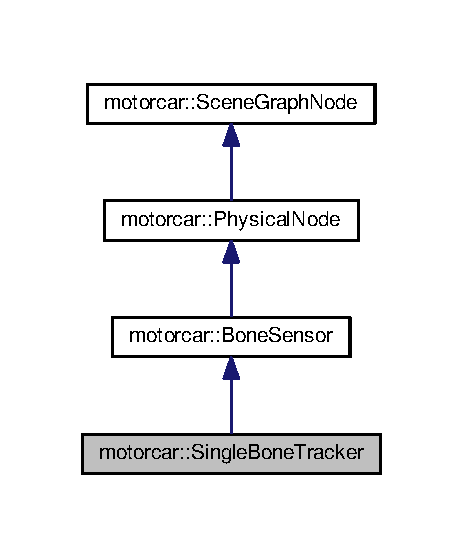
\includegraphics[width=222pt]{classmotorcar_1_1SingleBoneTracker__inherit__graph}
\end{center}
\end{figure}


Collaboration diagram for motorcar\-:\-:Single\-Bone\-Tracker\-:
\nopagebreak
\begin{figure}[H]
\begin{center}
\leavevmode
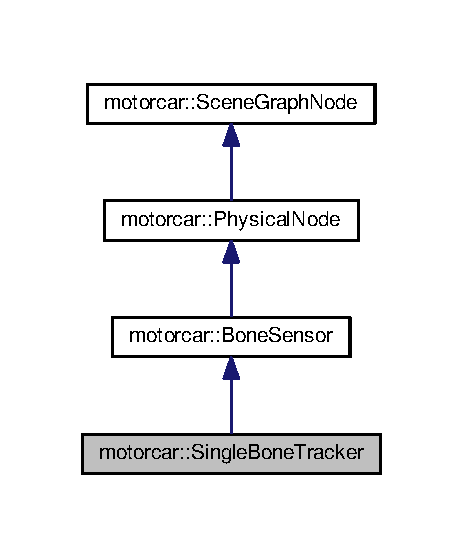
\includegraphics[width=222pt]{classmotorcar_1_1SingleBoneTracker__coll__graph}
\end{center}
\end{figure}
\subsection*{Public Member Functions}
\begin{DoxyCompactItemize}
\item 
\hyperlink{classmotorcar_1_1SingleBoneTracker_a8e95dd11e004f2b2610d2f92c86d1b60}{Single\-Bone\-Tracker} (\hyperlink{classmotorcar_1_1Bone}{Bone} $\ast$\hyperlink{classmotorcar_1_1SingleBoneTracker_abb942351d9129aca1307bedd3da54a13}{tracked\-Bone}, glm\-::mat4 \hyperlink{classmotorcar_1_1SingleBoneTracker_a2e4fa7ee58217a38f001091f1d3f8d8f}{bone\-Track\-Transform}, \hyperlink{classmotorcar_1_1Skeleton}{Skeleton} $\ast$\hyperlink{classmotorcar_1_1BoneSensor_a71f19e3ae5fac133a9f359c5ba4cef00}{skeleton}, \hyperlink{classmotorcar_1_1PhysicalNode}{Physical\-Node} $\ast$parent, const glm\-::mat4 \&\hyperlink{classmotorcar_1_1SceneGraphNode_ad96e79fdd739ac8223a3128003be391a}{transform}=glm\-::mat4())
\item 
void \hyperlink{classmotorcar_1_1SingleBoneTracker_a66f25aca80c6c03d882369b3d1b40f77}{set\-Position} (const glm\-::vec3 \&position)
\begin{DoxyCompactList}\small\item\em Set the position of the tracker in parent space. \end{DoxyCompactList}\item 
void \hyperlink{classmotorcar_1_1SingleBoneTracker_a2ea129b1f4f2caec8bbb71c48108b794}{set\-Orientation} (const glm\-::mat3 \&orientation)
\begin{DoxyCompactList}\small\item\em Set the orientation of the tracker in parent space. \end{DoxyCompactList}\item 
\hyperlink{classmotorcar_1_1Bone}{Bone} $\ast$ \hyperlink{classmotorcar_1_1SingleBoneTracker_abb942351d9129aca1307bedd3da54a13}{tracked\-Bone} () const 
\begin{DoxyCompactList}\small\item\em Gets the bone that this tracker is attached to. \end{DoxyCompactList}\item 
void \hyperlink{classmotorcar_1_1SingleBoneTracker_a5d508397b62585d59a702fbe37db94ef}{set\-Tracked\-Bone} (\hyperlink{classmotorcar_1_1Bone}{Bone} $\ast$\hyperlink{classmotorcar_1_1SingleBoneTracker_abb942351d9129aca1307bedd3da54a13}{tracked\-Bone})
\begin{DoxyCompactList}\small\item\em Sets the bone that this tracker is attached to. \end{DoxyCompactList}\item 
glm\-::mat4 \hyperlink{classmotorcar_1_1SingleBoneTracker_a2e4fa7ee58217a38f001091f1d3f8d8f}{bone\-Track\-Transform} () const 
\begin{DoxyCompactList}\small\item\em Gets the transform that describes how this tracker is attached to the bone it tracks. \end{DoxyCompactList}\item 
void \hyperlink{classmotorcar_1_1SingleBoneTracker_a20fb4b211211d7d1e9d2659031377482}{set\-Bone\-Track\-Transform} (const glm\-::mat4 \&\hyperlink{classmotorcar_1_1SingleBoneTracker_a2e4fa7ee58217a38f001091f1d3f8d8f}{bone\-Track\-Transform})
\begin{DoxyCompactList}\small\item\em Sets the transform that describes how this tracker is attached to the bone it tracks. \end{DoxyCompactList}\end{DoxyCompactItemize}
\subsection*{Additional Inherited Members}


\subsection{Constructor \& Destructor Documentation}
\hypertarget{classmotorcar_1_1SingleBoneTracker_a8e95dd11e004f2b2610d2f92c86d1b60}{\index{motorcar\-::\-Single\-Bone\-Tracker@{motorcar\-::\-Single\-Bone\-Tracker}!Single\-Bone\-Tracker@{Single\-Bone\-Tracker}}
\index{Single\-Bone\-Tracker@{Single\-Bone\-Tracker}!motorcar::SingleBoneTracker@{motorcar\-::\-Single\-Bone\-Tracker}}
\subsubsection[{Single\-Bone\-Tracker}]{\setlength{\rightskip}{0pt plus 5cm}Single\-Bone\-Tracker\-::\-Single\-Bone\-Tracker (
\begin{DoxyParamCaption}
\item[{{\bf Bone} $\ast$}]{tracked\-Bone, }
\item[{glm\-::mat4}]{bone\-Track\-Transform, }
\item[{{\bf Skeleton} $\ast$}]{skeleton, }
\item[{{\bf Physical\-Node} $\ast$}]{parent, }
\item[{const glm\-::mat4 \&}]{transform = {\ttfamily glm\-:\-:mat4()}}
\end{DoxyParamCaption}
)}}\label{classmotorcar_1_1SingleBoneTracker_a8e95dd11e004f2b2610d2f92c86d1b60}


\subsection{Member Function Documentation}
\hypertarget{classmotorcar_1_1SingleBoneTracker_a2e4fa7ee58217a38f001091f1d3f8d8f}{\index{motorcar\-::\-Single\-Bone\-Tracker@{motorcar\-::\-Single\-Bone\-Tracker}!bone\-Track\-Transform@{bone\-Track\-Transform}}
\index{bone\-Track\-Transform@{bone\-Track\-Transform}!motorcar::SingleBoneTracker@{motorcar\-::\-Single\-Bone\-Tracker}}
\subsubsection[{bone\-Track\-Transform}]{\setlength{\rightskip}{0pt plus 5cm}glm\-::mat4 Single\-Bone\-Tracker\-::bone\-Track\-Transform (
\begin{DoxyParamCaption}
{}
\end{DoxyParamCaption}
) const}}\label{classmotorcar_1_1SingleBoneTracker_a2e4fa7ee58217a38f001091f1d3f8d8f}


Gets the transform that describes how this tracker is attached to the bone it tracks. 

\hypertarget{classmotorcar_1_1SingleBoneTracker_a20fb4b211211d7d1e9d2659031377482}{\index{motorcar\-::\-Single\-Bone\-Tracker@{motorcar\-::\-Single\-Bone\-Tracker}!set\-Bone\-Track\-Transform@{set\-Bone\-Track\-Transform}}
\index{set\-Bone\-Track\-Transform@{set\-Bone\-Track\-Transform}!motorcar::SingleBoneTracker@{motorcar\-::\-Single\-Bone\-Tracker}}
\subsubsection[{set\-Bone\-Track\-Transform}]{\setlength{\rightskip}{0pt plus 5cm}void Single\-Bone\-Tracker\-::set\-Bone\-Track\-Transform (
\begin{DoxyParamCaption}
\item[{const glm\-::mat4 \&}]{bone\-Track\-Transform}
\end{DoxyParamCaption}
)}}\label{classmotorcar_1_1SingleBoneTracker_a20fb4b211211d7d1e9d2659031377482}


Sets the transform that describes how this tracker is attached to the bone it tracks. 

\hypertarget{classmotorcar_1_1SingleBoneTracker_a2ea129b1f4f2caec8bbb71c48108b794}{\index{motorcar\-::\-Single\-Bone\-Tracker@{motorcar\-::\-Single\-Bone\-Tracker}!set\-Orientation@{set\-Orientation}}
\index{set\-Orientation@{set\-Orientation}!motorcar::SingleBoneTracker@{motorcar\-::\-Single\-Bone\-Tracker}}
\subsubsection[{set\-Orientation}]{\setlength{\rightskip}{0pt plus 5cm}void Single\-Bone\-Tracker\-::set\-Orientation (
\begin{DoxyParamCaption}
\item[{const glm\-::mat3 \&}]{orientation}
\end{DoxyParamCaption}
)}}\label{classmotorcar_1_1SingleBoneTracker_a2ea129b1f4f2caec8bbb71c48108b794}


Set the orientation of the tracker in parent space. 

\hypertarget{classmotorcar_1_1SingleBoneTracker_a66f25aca80c6c03d882369b3d1b40f77}{\index{motorcar\-::\-Single\-Bone\-Tracker@{motorcar\-::\-Single\-Bone\-Tracker}!set\-Position@{set\-Position}}
\index{set\-Position@{set\-Position}!motorcar::SingleBoneTracker@{motorcar\-::\-Single\-Bone\-Tracker}}
\subsubsection[{set\-Position}]{\setlength{\rightskip}{0pt plus 5cm}void Single\-Bone\-Tracker\-::set\-Position (
\begin{DoxyParamCaption}
\item[{const glm\-::vec3 \&}]{position}
\end{DoxyParamCaption}
)}}\label{classmotorcar_1_1SingleBoneTracker_a66f25aca80c6c03d882369b3d1b40f77}


Set the position of the tracker in parent space. 

\hypertarget{classmotorcar_1_1SingleBoneTracker_a5d508397b62585d59a702fbe37db94ef}{\index{motorcar\-::\-Single\-Bone\-Tracker@{motorcar\-::\-Single\-Bone\-Tracker}!set\-Tracked\-Bone@{set\-Tracked\-Bone}}
\index{set\-Tracked\-Bone@{set\-Tracked\-Bone}!motorcar::SingleBoneTracker@{motorcar\-::\-Single\-Bone\-Tracker}}
\subsubsection[{set\-Tracked\-Bone}]{\setlength{\rightskip}{0pt plus 5cm}void Single\-Bone\-Tracker\-::set\-Tracked\-Bone (
\begin{DoxyParamCaption}
\item[{{\bf Bone} $\ast$}]{tracked\-Bone}
\end{DoxyParamCaption}
)}}\label{classmotorcar_1_1SingleBoneTracker_a5d508397b62585d59a702fbe37db94ef}


Sets the bone that this tracker is attached to. 

\hypertarget{classmotorcar_1_1SingleBoneTracker_abb942351d9129aca1307bedd3da54a13}{\index{motorcar\-::\-Single\-Bone\-Tracker@{motorcar\-::\-Single\-Bone\-Tracker}!tracked\-Bone@{tracked\-Bone}}
\index{tracked\-Bone@{tracked\-Bone}!motorcar::SingleBoneTracker@{motorcar\-::\-Single\-Bone\-Tracker}}
\subsubsection[{tracked\-Bone}]{\setlength{\rightskip}{0pt plus 5cm}{\bf Bone} $\ast$ Single\-Bone\-Tracker\-::tracked\-Bone (
\begin{DoxyParamCaption}
{}
\end{DoxyParamCaption}
) const}}\label{classmotorcar_1_1SingleBoneTracker_abb942351d9129aca1307bedd3da54a13}


Gets the bone that this tracker is attached to. 



The documentation for this class was generated from the following files\-:\begin{DoxyCompactItemize}
\item 
/home/dave/thesis/motorcar/src/compositor/scenegraph/input/\hyperlink{singlebonetracker_8h}{singlebonetracker.\-h}\item 
/home/dave/thesis/motorcar/src/compositor/scenegraph/input/\hyperlink{singlebonetracker_8cpp}{singlebonetracker.\-cpp}\end{DoxyCompactItemize}

\hypertarget{classmotorcar_1_1SixDofEvent}{\section{motorcar\-:\-:Six\-Dof\-Event Class Reference}
\label{classmotorcar_1_1SixDofEvent}\index{motorcar\-::\-Six\-Dof\-Event@{motorcar\-::\-Six\-Dof\-Event}}
}


{\ttfamily \#include $<$sixdofevent.\-h$>$}



Inheritance diagram for motorcar\-:\-:Six\-Dof\-Event\-:
\nopagebreak
\begin{figure}[H]
\begin{center}
\leavevmode
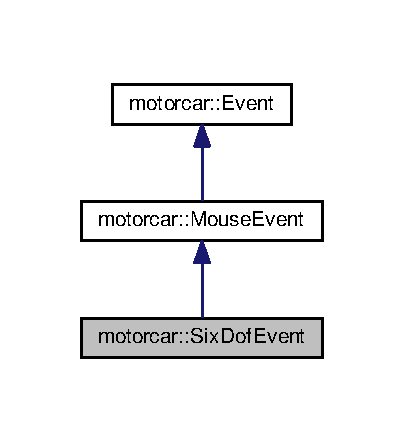
\includegraphics[width=194pt]{classmotorcar_1_1SixDofEvent__inherit__graph}
\end{center}
\end{figure}


Collaboration diagram for motorcar\-:\-:Six\-Dof\-Event\-:
\nopagebreak
\begin{figure}[H]
\begin{center}
\leavevmode
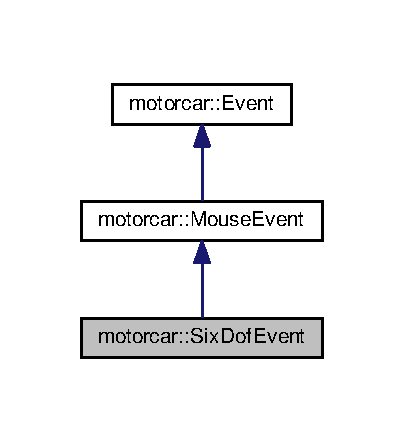
\includegraphics[width=194pt]{classmotorcar_1_1SixDofEvent__coll__graph}
\end{center}
\end{figure}
\subsection*{Public Member Functions}
\begin{DoxyCompactItemize}
\item 
\hyperlink{classmotorcar_1_1SixDofEvent_a5a037950efd8c7cf70dc7a69ce700d48}{Six\-Dof\-Event} (\hyperlink{classmotorcar_1_1MouseEvent_a2d063fb053a90c196b58c1dec4d989aa}{Mouse\-Event\-::\-Event} \hyperlink{classmotorcar_1_1MouseEvent_a52d0060d0793eab0ca6aad7f69d78fda}{event}, \hyperlink{classmotorcar_1_1MouseEvent_aeb5515c2434123ce2f897f8fc89effae}{Mouse\-Event\-::\-Button} \hyperlink{classmotorcar_1_1MouseEvent_a6682d4092f940335170806435e3bb6fe}{button}, \hyperlink{classmotorcar_1_1Seat}{Seat} $\ast$\hyperlink{classmotorcar_1_1Event_a7426828c8402193cac63a7b3fda5a17e}{seat}, glm\-::mat4 \hyperlink{classmotorcar_1_1SixDofEvent_a96aeaea9499f4d7f8980178a17fc9533}{transform})
\item 
glm\-::mat4 \hyperlink{classmotorcar_1_1SixDofEvent_a96aeaea9499f4d7f8980178a17fc9533}{transform} () const 
\end{DoxyCompactItemize}
\subsection*{Additional Inherited Members}


\subsection{Constructor \& Destructor Documentation}
\hypertarget{classmotorcar_1_1SixDofEvent_a5a037950efd8c7cf70dc7a69ce700d48}{\index{motorcar\-::\-Six\-Dof\-Event@{motorcar\-::\-Six\-Dof\-Event}!Six\-Dof\-Event@{Six\-Dof\-Event}}
\index{Six\-Dof\-Event@{Six\-Dof\-Event}!motorcar::SixDofEvent@{motorcar\-::\-Six\-Dof\-Event}}
\subsubsection[{Six\-Dof\-Event}]{\setlength{\rightskip}{0pt plus 5cm}Six\-Dof\-Event\-::\-Six\-Dof\-Event (
\begin{DoxyParamCaption}
\item[{{\bf Mouse\-Event\-::\-Event}}]{event, }
\item[{{\bf Mouse\-Event\-::\-Button}}]{button, }
\item[{{\bf Seat} $\ast$}]{seat, }
\item[{glm\-::mat4}]{transform}
\end{DoxyParamCaption}
)}}\label{classmotorcar_1_1SixDofEvent_a5a037950efd8c7cf70dc7a69ce700d48}


\subsection{Member Function Documentation}
\hypertarget{classmotorcar_1_1SixDofEvent_a96aeaea9499f4d7f8980178a17fc9533}{\index{motorcar\-::\-Six\-Dof\-Event@{motorcar\-::\-Six\-Dof\-Event}!transform@{transform}}
\index{transform@{transform}!motorcar::SixDofEvent@{motorcar\-::\-Six\-Dof\-Event}}
\subsubsection[{transform}]{\setlength{\rightskip}{0pt plus 5cm}glm\-::mat4 Six\-Dof\-Event\-::transform (
\begin{DoxyParamCaption}
{}
\end{DoxyParamCaption}
) const}}\label{classmotorcar_1_1SixDofEvent_a96aeaea9499f4d7f8980178a17fc9533}


The documentation for this class was generated from the following files\-:\begin{DoxyCompactItemize}
\item 
/home/dave/thesis/motorcar/src/compositor/events/\hyperlink{sixdofevent_8h}{sixdofevent.\-h}\item 
/home/dave/thesis/motorcar/src/compositor/events/\hyperlink{sixdofevent_8cpp}{sixdofevent.\-cpp}\end{DoxyCompactItemize}

\hypertarget{classsixDofPointer}{\section{six\-Dof\-Pointer Class Reference}
\label{classsixDofPointer}\index{six\-Dof\-Pointer@{six\-Dof\-Pointer}}
}
\subsection*{Public Attributes}
\begin{DoxyCompactItemize}
\item 
glm\-::mat4 \hyperlink{classsixDofPointer_ab3bb1b8ac72a9d575265f454d43ada9f}{transform}
\end{DoxyCompactItemize}


\subsection{Member Data Documentation}
\hypertarget{classsixDofPointer_ab3bb1b8ac72a9d575265f454d43ada9f}{\index{six\-Dof\-Pointer@{six\-Dof\-Pointer}!transform@{transform}}
\index{transform@{transform}!sixDofPointer@{six\-Dof\-Pointer}}
\subsubsection[{transform}]{\setlength{\rightskip}{0pt plus 5cm}glm\-::mat4 six\-Dof\-Pointer\-::transform}}\label{classsixDofPointer_ab3bb1b8ac72a9d575265f454d43ada9f}


The documentation for this class was generated from the following file\-:\begin{DoxyCompactItemize}
\item 
/home/dave/thesis/motorcar/src/examples/clients/simple-\/egl/\hyperlink{simple-egl_8cpp}{simple-\/egl.\-cpp}\end{DoxyCompactItemize}

\hypertarget{classmotorcar_1_1SixDOFPointingDevice}{\section{motorcar\-:\-:Six\-D\-O\-F\-Pointing\-Device Class Reference}
\label{classmotorcar_1_1SixDOFPointingDevice}\index{motorcar\-::\-Six\-D\-O\-F\-Pointing\-Device@{motorcar\-::\-Six\-D\-O\-F\-Pointing\-Device}}
}


{\ttfamily \#include $<$sixdofpointingdevice.\-h$>$}



Inheritance diagram for motorcar\-:\-:Six\-D\-O\-F\-Pointing\-Device\-:
\nopagebreak
\begin{figure}[H]
\begin{center}
\leavevmode
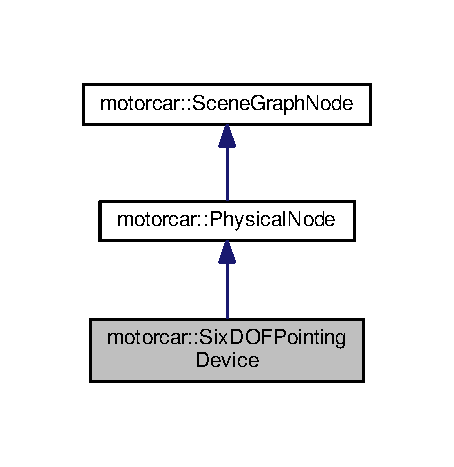
\includegraphics[width=218pt]{classmotorcar_1_1SixDOFPointingDevice__inherit__graph}
\end{center}
\end{figure}


Collaboration diagram for motorcar\-:\-:Six\-D\-O\-F\-Pointing\-Device\-:
\nopagebreak
\begin{figure}[H]
\begin{center}
\leavevmode
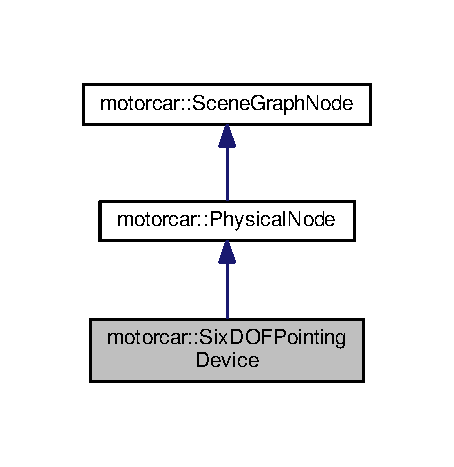
\includegraphics[width=218pt]{classmotorcar_1_1SixDOFPointingDevice__coll__graph}
\end{center}
\end{figure}
\subsection*{Public Member Functions}
\begin{DoxyCompactItemize}
\item 
\hyperlink{classmotorcar_1_1SixDOFPointingDevice_a553ef70ad5a67e2f21a012a57c7fc398}{Six\-D\-O\-F\-Pointing\-Device} (\hyperlink{classmotorcar_1_1Seat}{Seat} $\ast$\hyperlink{classmotorcar_1_1SixDOFPointingDevice_a296fe215aeb4ae2e8724c877aabc874f}{seat}, \hyperlink{classmotorcar_1_1PhysicalNode}{Physical\-Node} $\ast$parent, const glm\-::mat4 \&\hyperlink{classmotorcar_1_1SceneGraphNode_ad96e79fdd739ac8223a3128003be391a}{transform}=glm\-::mat4())
\item 
virtual \hyperlink{classmotorcar_1_1SixDOFPointingDevice_a234bf04e5af6be0f832f0a425719273c}{$\sim$\-Six\-D\-O\-F\-Pointing\-Device} ()
\item 
virtual void \hyperlink{classmotorcar_1_1SixDOFPointingDevice_a70dad2fa3cc63cb6eac584ae2f632df6}{handle\-Frame\-Begin} (\hyperlink{classmotorcar_1_1Scene}{Scene} $\ast$\hyperlink{classmotorcar_1_1SceneGraphNode_aa14e637ed4ae98f77e28941a4b5cfdd8}{scene}) override
\begin{DoxyCompactList}\small\item\em updates the current device state and moves any attaches surfaces \end{DoxyCompactList}\item 
bool \hyperlink{classmotorcar_1_1SixDOFPointingDevice_a7d73caedee587fab53c19e4ee1617611}{left\-Mouse\-Down} () const 
\item 
void \hyperlink{classmotorcar_1_1SixDOFPointingDevice_a8f3f87d7e7f64991d3abb6e724ca25be}{set\-Left\-Mouse\-Down} (bool \hyperlink{classmotorcar_1_1SixDOFPointingDevice_a7d73caedee587fab53c19e4ee1617611}{left\-Mouse\-Down})
\item 
bool \hyperlink{classmotorcar_1_1SixDOFPointingDevice_a832aeb89ec4400f0c32c6ba355d5a3f4}{right\-Mouse\-Down} () const 
\item 
void \hyperlink{classmotorcar_1_1SixDOFPointingDevice_ac4cf201773bef4db5f57dedfbb8ca0c1}{set\-Right\-Mouse\-Down} (bool \hyperlink{classmotorcar_1_1SixDOFPointingDevice_a832aeb89ec4400f0c32c6ba355d5a3f4}{right\-Mouse\-Down})
\item 
bool \hyperlink{classmotorcar_1_1SixDOFPointingDevice_a85585b2c17d6457206616f0ac6e5479c}{middle\-Mouse\-Down} () const 
\item 
void \hyperlink{classmotorcar_1_1SixDOFPointingDevice_a3f5b831a8731fd60ce01e5066319f09f}{set\-Middle\-Mouse\-Down} (bool \hyperlink{classmotorcar_1_1SixDOFPointingDevice_a85585b2c17d6457206616f0ac6e5479c}{middle\-Mouse\-Down})
\item 
void \hyperlink{classmotorcar_1_1SixDOFPointingDevice_a9b55d485a1870d9e50aa85ac3396252c}{grab\-Surface\-Under\-Cursor} ()
\item 
void \hyperlink{classmotorcar_1_1SixDOFPointingDevice_a058f434cd85dc2b722f752122e6ce49f}{release\-Grabbed\-Surface} ()
\item 
\hyperlink{classmotorcar_1_1Seat}{Seat} $\ast$ \hyperlink{classmotorcar_1_1SixDOFPointingDevice_a296fe215aeb4ae2e8724c877aabc874f}{seat} () const 
\item 
void \hyperlink{classmotorcar_1_1SixDOFPointingDevice_a1f97741dbf9f49b6b071558ac3f56b92}{set\-Seat} (\hyperlink{classmotorcar_1_1Seat}{Seat} $\ast$\hyperlink{classmotorcar_1_1SixDOFPointingDevice_a296fe215aeb4ae2e8724c877aabc874f}{seat})
\item 
struct wl\-\_\-resource $\ast$ \hyperlink{classmotorcar_1_1SixDOFPointingDevice_a091a631f8fa2adfab8d0a7904cd47eb5}{resource\-For\-Client} (struct wl\-\_\-client $\ast$client)
\end{DoxyCompactItemize}
\subsection*{Additional Inherited Members}


\subsection{Constructor \& Destructor Documentation}
\hypertarget{classmotorcar_1_1SixDOFPointingDevice_a553ef70ad5a67e2f21a012a57c7fc398}{\index{motorcar\-::\-Six\-D\-O\-F\-Pointing\-Device@{motorcar\-::\-Six\-D\-O\-F\-Pointing\-Device}!Six\-D\-O\-F\-Pointing\-Device@{Six\-D\-O\-F\-Pointing\-Device}}
\index{Six\-D\-O\-F\-Pointing\-Device@{Six\-D\-O\-F\-Pointing\-Device}!motorcar::SixDOFPointingDevice@{motorcar\-::\-Six\-D\-O\-F\-Pointing\-Device}}
\subsubsection[{Six\-D\-O\-F\-Pointing\-Device}]{\setlength{\rightskip}{0pt plus 5cm}Six\-D\-O\-F\-Pointing\-Device\-::\-Six\-D\-O\-F\-Pointing\-Device (
\begin{DoxyParamCaption}
\item[{{\bf Seat} $\ast$}]{seat, }
\item[{{\bf Physical\-Node} $\ast$}]{parent, }
\item[{const glm\-::mat4 \&}]{transform = {\ttfamily glm\-:\-:mat4()}}
\end{DoxyParamCaption}
)}}\label{classmotorcar_1_1SixDOFPointingDevice_a553ef70ad5a67e2f21a012a57c7fc398}
\hypertarget{classmotorcar_1_1SixDOFPointingDevice_a234bf04e5af6be0f832f0a425719273c}{\index{motorcar\-::\-Six\-D\-O\-F\-Pointing\-Device@{motorcar\-::\-Six\-D\-O\-F\-Pointing\-Device}!$\sim$\-Six\-D\-O\-F\-Pointing\-Device@{$\sim$\-Six\-D\-O\-F\-Pointing\-Device}}
\index{$\sim$\-Six\-D\-O\-F\-Pointing\-Device@{$\sim$\-Six\-D\-O\-F\-Pointing\-Device}!motorcar::SixDOFPointingDevice@{motorcar\-::\-Six\-D\-O\-F\-Pointing\-Device}}
\subsubsection[{$\sim$\-Six\-D\-O\-F\-Pointing\-Device}]{\setlength{\rightskip}{0pt plus 5cm}virtual motorcar\-::\-Six\-D\-O\-F\-Pointing\-Device\-::$\sim$\-Six\-D\-O\-F\-Pointing\-Device (
\begin{DoxyParamCaption}
{}
\end{DoxyParamCaption}
)\hspace{0.3cm}{\ttfamily [inline]}, {\ttfamily [virtual]}}}\label{classmotorcar_1_1SixDOFPointingDevice_a234bf04e5af6be0f832f0a425719273c}


\subsection{Member Function Documentation}
\hypertarget{classmotorcar_1_1SixDOFPointingDevice_a9b55d485a1870d9e50aa85ac3396252c}{\index{motorcar\-::\-Six\-D\-O\-F\-Pointing\-Device@{motorcar\-::\-Six\-D\-O\-F\-Pointing\-Device}!grab\-Surface\-Under\-Cursor@{grab\-Surface\-Under\-Cursor}}
\index{grab\-Surface\-Under\-Cursor@{grab\-Surface\-Under\-Cursor}!motorcar::SixDOFPointingDevice@{motorcar\-::\-Six\-D\-O\-F\-Pointing\-Device}}
\subsubsection[{grab\-Surface\-Under\-Cursor}]{\setlength{\rightskip}{0pt plus 5cm}void Six\-D\-O\-F\-Pointing\-Device\-::grab\-Surface\-Under\-Cursor (
\begin{DoxyParamCaption}
{}
\end{DoxyParamCaption}
)}}\label{classmotorcar_1_1SixDOFPointingDevice_a9b55d485a1870d9e50aa85ac3396252c}
\hypertarget{classmotorcar_1_1SixDOFPointingDevice_a70dad2fa3cc63cb6eac584ae2f632df6}{\index{motorcar\-::\-Six\-D\-O\-F\-Pointing\-Device@{motorcar\-::\-Six\-D\-O\-F\-Pointing\-Device}!handle\-Frame\-Begin@{handle\-Frame\-Begin}}
\index{handle\-Frame\-Begin@{handle\-Frame\-Begin}!motorcar::SixDOFPointingDevice@{motorcar\-::\-Six\-D\-O\-F\-Pointing\-Device}}
\subsubsection[{handle\-Frame\-Begin}]{\setlength{\rightskip}{0pt plus 5cm}void Six\-D\-O\-F\-Pointing\-Device\-::handle\-Frame\-Begin (
\begin{DoxyParamCaption}
\item[{{\bf Scene} $\ast$}]{scene}
\end{DoxyParamCaption}
)\hspace{0.3cm}{\ttfamily [override]}, {\ttfamily [virtual]}}}\label{classmotorcar_1_1SixDOFPointingDevice_a70dad2fa3cc63cb6eac584ae2f632df6}


updates the current device state and moves any attaches surfaces 



Reimplemented from \hyperlink{classmotorcar_1_1SceneGraphNode_a494eb20dd66a224888237af89ba6956f}{motorcar\-::\-Scene\-Graph\-Node}.

\hypertarget{classmotorcar_1_1SixDOFPointingDevice_a7d73caedee587fab53c19e4ee1617611}{\index{motorcar\-::\-Six\-D\-O\-F\-Pointing\-Device@{motorcar\-::\-Six\-D\-O\-F\-Pointing\-Device}!left\-Mouse\-Down@{left\-Mouse\-Down}}
\index{left\-Mouse\-Down@{left\-Mouse\-Down}!motorcar::SixDOFPointingDevice@{motorcar\-::\-Six\-D\-O\-F\-Pointing\-Device}}
\subsubsection[{left\-Mouse\-Down}]{\setlength{\rightskip}{0pt plus 5cm}bool Six\-D\-O\-F\-Pointing\-Device\-::left\-Mouse\-Down (
\begin{DoxyParamCaption}
{}
\end{DoxyParamCaption}
) const}}\label{classmotorcar_1_1SixDOFPointingDevice_a7d73caedee587fab53c19e4ee1617611}
\hypertarget{classmotorcar_1_1SixDOFPointingDevice_a85585b2c17d6457206616f0ac6e5479c}{\index{motorcar\-::\-Six\-D\-O\-F\-Pointing\-Device@{motorcar\-::\-Six\-D\-O\-F\-Pointing\-Device}!middle\-Mouse\-Down@{middle\-Mouse\-Down}}
\index{middle\-Mouse\-Down@{middle\-Mouse\-Down}!motorcar::SixDOFPointingDevice@{motorcar\-::\-Six\-D\-O\-F\-Pointing\-Device}}
\subsubsection[{middle\-Mouse\-Down}]{\setlength{\rightskip}{0pt plus 5cm}bool Six\-D\-O\-F\-Pointing\-Device\-::middle\-Mouse\-Down (
\begin{DoxyParamCaption}
{}
\end{DoxyParamCaption}
) const}}\label{classmotorcar_1_1SixDOFPointingDevice_a85585b2c17d6457206616f0ac6e5479c}
\hypertarget{classmotorcar_1_1SixDOFPointingDevice_a058f434cd85dc2b722f752122e6ce49f}{\index{motorcar\-::\-Six\-D\-O\-F\-Pointing\-Device@{motorcar\-::\-Six\-D\-O\-F\-Pointing\-Device}!release\-Grabbed\-Surface@{release\-Grabbed\-Surface}}
\index{release\-Grabbed\-Surface@{release\-Grabbed\-Surface}!motorcar::SixDOFPointingDevice@{motorcar\-::\-Six\-D\-O\-F\-Pointing\-Device}}
\subsubsection[{release\-Grabbed\-Surface}]{\setlength{\rightskip}{0pt plus 5cm}void Six\-D\-O\-F\-Pointing\-Device\-::release\-Grabbed\-Surface (
\begin{DoxyParamCaption}
{}
\end{DoxyParamCaption}
)}}\label{classmotorcar_1_1SixDOFPointingDevice_a058f434cd85dc2b722f752122e6ce49f}
\hypertarget{classmotorcar_1_1SixDOFPointingDevice_a091a631f8fa2adfab8d0a7904cd47eb5}{\index{motorcar\-::\-Six\-D\-O\-F\-Pointing\-Device@{motorcar\-::\-Six\-D\-O\-F\-Pointing\-Device}!resource\-For\-Client@{resource\-For\-Client}}
\index{resource\-For\-Client@{resource\-For\-Client}!motorcar::SixDOFPointingDevice@{motorcar\-::\-Six\-D\-O\-F\-Pointing\-Device}}
\subsubsection[{resource\-For\-Client}]{\setlength{\rightskip}{0pt plus 5cm}wl\-\_\-resource $\ast$ Six\-D\-O\-F\-Pointing\-Device\-::resource\-For\-Client (
\begin{DoxyParamCaption}
\item[{struct wl\-\_\-client $\ast$}]{client}
\end{DoxyParamCaption}
)}}\label{classmotorcar_1_1SixDOFPointingDevice_a091a631f8fa2adfab8d0a7904cd47eb5}
\hypertarget{classmotorcar_1_1SixDOFPointingDevice_a832aeb89ec4400f0c32c6ba355d5a3f4}{\index{motorcar\-::\-Six\-D\-O\-F\-Pointing\-Device@{motorcar\-::\-Six\-D\-O\-F\-Pointing\-Device}!right\-Mouse\-Down@{right\-Mouse\-Down}}
\index{right\-Mouse\-Down@{right\-Mouse\-Down}!motorcar::SixDOFPointingDevice@{motorcar\-::\-Six\-D\-O\-F\-Pointing\-Device}}
\subsubsection[{right\-Mouse\-Down}]{\setlength{\rightskip}{0pt plus 5cm}bool Six\-D\-O\-F\-Pointing\-Device\-::right\-Mouse\-Down (
\begin{DoxyParamCaption}
{}
\end{DoxyParamCaption}
) const}}\label{classmotorcar_1_1SixDOFPointingDevice_a832aeb89ec4400f0c32c6ba355d5a3f4}
\hypertarget{classmotorcar_1_1SixDOFPointingDevice_a296fe215aeb4ae2e8724c877aabc874f}{\index{motorcar\-::\-Six\-D\-O\-F\-Pointing\-Device@{motorcar\-::\-Six\-D\-O\-F\-Pointing\-Device}!seat@{seat}}
\index{seat@{seat}!motorcar::SixDOFPointingDevice@{motorcar\-::\-Six\-D\-O\-F\-Pointing\-Device}}
\subsubsection[{seat}]{\setlength{\rightskip}{0pt plus 5cm}{\bf Seat} $\ast$ Six\-D\-O\-F\-Pointing\-Device\-::seat (
\begin{DoxyParamCaption}
{}
\end{DoxyParamCaption}
) const}}\label{classmotorcar_1_1SixDOFPointingDevice_a296fe215aeb4ae2e8724c877aabc874f}
\hypertarget{classmotorcar_1_1SixDOFPointingDevice_a8f3f87d7e7f64991d3abb6e724ca25be}{\index{motorcar\-::\-Six\-D\-O\-F\-Pointing\-Device@{motorcar\-::\-Six\-D\-O\-F\-Pointing\-Device}!set\-Left\-Mouse\-Down@{set\-Left\-Mouse\-Down}}
\index{set\-Left\-Mouse\-Down@{set\-Left\-Mouse\-Down}!motorcar::SixDOFPointingDevice@{motorcar\-::\-Six\-D\-O\-F\-Pointing\-Device}}
\subsubsection[{set\-Left\-Mouse\-Down}]{\setlength{\rightskip}{0pt plus 5cm}void Six\-D\-O\-F\-Pointing\-Device\-::set\-Left\-Mouse\-Down (
\begin{DoxyParamCaption}
\item[{bool}]{left\-Mouse\-Down}
\end{DoxyParamCaption}
)}}\label{classmotorcar_1_1SixDOFPointingDevice_a8f3f87d7e7f64991d3abb6e724ca25be}
\hypertarget{classmotorcar_1_1SixDOFPointingDevice_a3f5b831a8731fd60ce01e5066319f09f}{\index{motorcar\-::\-Six\-D\-O\-F\-Pointing\-Device@{motorcar\-::\-Six\-D\-O\-F\-Pointing\-Device}!set\-Middle\-Mouse\-Down@{set\-Middle\-Mouse\-Down}}
\index{set\-Middle\-Mouse\-Down@{set\-Middle\-Mouse\-Down}!motorcar::SixDOFPointingDevice@{motorcar\-::\-Six\-D\-O\-F\-Pointing\-Device}}
\subsubsection[{set\-Middle\-Mouse\-Down}]{\setlength{\rightskip}{0pt plus 5cm}void Six\-D\-O\-F\-Pointing\-Device\-::set\-Middle\-Mouse\-Down (
\begin{DoxyParamCaption}
\item[{bool}]{middle\-Mouse\-Down}
\end{DoxyParamCaption}
)}}\label{classmotorcar_1_1SixDOFPointingDevice_a3f5b831a8731fd60ce01e5066319f09f}
\hypertarget{classmotorcar_1_1SixDOFPointingDevice_ac4cf201773bef4db5f57dedfbb8ca0c1}{\index{motorcar\-::\-Six\-D\-O\-F\-Pointing\-Device@{motorcar\-::\-Six\-D\-O\-F\-Pointing\-Device}!set\-Right\-Mouse\-Down@{set\-Right\-Mouse\-Down}}
\index{set\-Right\-Mouse\-Down@{set\-Right\-Mouse\-Down}!motorcar::SixDOFPointingDevice@{motorcar\-::\-Six\-D\-O\-F\-Pointing\-Device}}
\subsubsection[{set\-Right\-Mouse\-Down}]{\setlength{\rightskip}{0pt plus 5cm}void Six\-D\-O\-F\-Pointing\-Device\-::set\-Right\-Mouse\-Down (
\begin{DoxyParamCaption}
\item[{bool}]{right\-Mouse\-Down}
\end{DoxyParamCaption}
)}}\label{classmotorcar_1_1SixDOFPointingDevice_ac4cf201773bef4db5f57dedfbb8ca0c1}
\hypertarget{classmotorcar_1_1SixDOFPointingDevice_a1f97741dbf9f49b6b071558ac3f56b92}{\index{motorcar\-::\-Six\-D\-O\-F\-Pointing\-Device@{motorcar\-::\-Six\-D\-O\-F\-Pointing\-Device}!set\-Seat@{set\-Seat}}
\index{set\-Seat@{set\-Seat}!motorcar::SixDOFPointingDevice@{motorcar\-::\-Six\-D\-O\-F\-Pointing\-Device}}
\subsubsection[{set\-Seat}]{\setlength{\rightskip}{0pt plus 5cm}void Six\-D\-O\-F\-Pointing\-Device\-::set\-Seat (
\begin{DoxyParamCaption}
\item[{{\bf Seat} $\ast$}]{seat}
\end{DoxyParamCaption}
)}}\label{classmotorcar_1_1SixDOFPointingDevice_a1f97741dbf9f49b6b071558ac3f56b92}


The documentation for this class was generated from the following files\-:\begin{DoxyCompactItemize}
\item 
/home/dave/thesis/motorcar/src/compositor/scenegraph/input/\hyperlink{sixdofpointingdevice_8h}{sixdofpointingdevice.\-h}\item 
/home/dave/thesis/motorcar/src/compositor/scenegraph/input/\hyperlink{sixdofpointingdevice_8cpp}{sixdofpointingdevice.\-cpp}\end{DoxyCompactItemize}

\hypertarget{classmotorcar_1_1SixenseBaseNode}{\section{motorcar\-:\-:Sixense\-Base\-Node Class Reference}
\label{classmotorcar_1_1SixenseBaseNode}\index{motorcar\-::\-Sixense\-Base\-Node@{motorcar\-::\-Sixense\-Base\-Node}}
}


{\ttfamily \#include $<$sixensebasenode.\-h$>$}



Inheritance diagram for motorcar\-:\-:Sixense\-Base\-Node\-:
\nopagebreak
\begin{figure}[H]
\begin{center}
\leavevmode
\includegraphics[width=222pt]{classmotorcar_1_1SixenseBaseNode__inherit__graph}
\end{center}
\end{figure}


Collaboration diagram for motorcar\-:\-:Sixense\-Base\-Node\-:
\nopagebreak
\begin{figure}[H]
\begin{center}
\leavevmode
\includegraphics[width=222pt]{classmotorcar_1_1SixenseBaseNode__coll__graph}
\end{center}
\end{figure}
\subsection*{Public Member Functions}
\begin{DoxyCompactItemize}
\item 
\hyperlink{classmotorcar_1_1SixenseBaseNode_a7d0d69617d419cda3837efaa2eaf2d2c}{Sixense\-Base\-Node} (int base\-Index, \hyperlink{classmotorcar_1_1PhysicalNode}{Physical\-Node} $\ast$parent, const glm\-::mat4 \&\hyperlink{classmotorcar_1_1SceneGraphNode_ad96e79fdd739ac8223a3128003be391a}{transform}=glm\-::mat4())
\item 
virtual void \hyperlink{classmotorcar_1_1SixenseBaseNode_a5f211241a5bf54194920582a8bb7e3c3}{handle\-Frame\-Begin} (\hyperlink{classmotorcar_1_1Scene}{Scene} $\ast$\hyperlink{classmotorcar_1_1SceneGraphNode_aa14e637ed4ae98f77e28941a4b5cfdd8}{scene}) override
\begin{DoxyCompactList}\small\item\em gets current system state and passes new controller state to controller nodes \end{DoxyCompactList}\item 
bool \hyperlink{classmotorcar_1_1SixenseBaseNode_a717b0bd837bfaa8a41330ff2e89fe818}{connected} () const 
\item 
void \hyperlink{classmotorcar_1_1SixenseBaseNode_adc93b3ae19192be4d4fbf39bfb5f954b}{set\-Connected} (bool \hyperlink{classmotorcar_1_1SixenseBaseNode_a717b0bd837bfaa8a41330ff2e89fe818}{connected})
\item 
std\-::vector\\*
$<$ \hyperlink{classmotorcar_1_1SixenseControllerNode}{Sixense\-Controller\-Node} $\ast$ $>$ \hyperlink{classmotorcar_1_1SixenseBaseNode_ac15f4bc8939447b77dfeda9749899acc}{controllers} () const 
\end{DoxyCompactItemize}
\subsection*{Additional Inherited Members}


\subsection{Constructor \& Destructor Documentation}
\hypertarget{classmotorcar_1_1SixenseBaseNode_a7d0d69617d419cda3837efaa2eaf2d2c}{\index{motorcar\-::\-Sixense\-Base\-Node@{motorcar\-::\-Sixense\-Base\-Node}!Sixense\-Base\-Node@{Sixense\-Base\-Node}}
\index{Sixense\-Base\-Node@{Sixense\-Base\-Node}!motorcar::SixenseBaseNode@{motorcar\-::\-Sixense\-Base\-Node}}
\subsubsection[{Sixense\-Base\-Node}]{\setlength{\rightskip}{0pt plus 5cm}Sixense\-Base\-Node\-::\-Sixense\-Base\-Node (
\begin{DoxyParamCaption}
\item[{int}]{base\-Index, }
\item[{{\bf Physical\-Node} $\ast$}]{parent, }
\item[{const glm\-::mat4 \&}]{transform = {\ttfamily glm\-:\-:mat4()}}
\end{DoxyParamCaption}
)}}\label{classmotorcar_1_1SixenseBaseNode_a7d0d69617d419cda3837efaa2eaf2d2c}


\subsection{Member Function Documentation}
\hypertarget{classmotorcar_1_1SixenseBaseNode_a717b0bd837bfaa8a41330ff2e89fe818}{\index{motorcar\-::\-Sixense\-Base\-Node@{motorcar\-::\-Sixense\-Base\-Node}!connected@{connected}}
\index{connected@{connected}!motorcar::SixenseBaseNode@{motorcar\-::\-Sixense\-Base\-Node}}
\subsubsection[{connected}]{\setlength{\rightskip}{0pt plus 5cm}bool Sixense\-Base\-Node\-::connected (
\begin{DoxyParamCaption}
{}
\end{DoxyParamCaption}
) const}}\label{classmotorcar_1_1SixenseBaseNode_a717b0bd837bfaa8a41330ff2e89fe818}
\hypertarget{classmotorcar_1_1SixenseBaseNode_ac15f4bc8939447b77dfeda9749899acc}{\index{motorcar\-::\-Sixense\-Base\-Node@{motorcar\-::\-Sixense\-Base\-Node}!controllers@{controllers}}
\index{controllers@{controllers}!motorcar::SixenseBaseNode@{motorcar\-::\-Sixense\-Base\-Node}}
\subsubsection[{controllers}]{\setlength{\rightskip}{0pt plus 5cm}std\-::vector$<$ {\bf Sixense\-Controller\-Node} $\ast$ $>$ Sixense\-Base\-Node\-::controllers (
\begin{DoxyParamCaption}
{}
\end{DoxyParamCaption}
) const}}\label{classmotorcar_1_1SixenseBaseNode_ac15f4bc8939447b77dfeda9749899acc}
\hypertarget{classmotorcar_1_1SixenseBaseNode_a5f211241a5bf54194920582a8bb7e3c3}{\index{motorcar\-::\-Sixense\-Base\-Node@{motorcar\-::\-Sixense\-Base\-Node}!handle\-Frame\-Begin@{handle\-Frame\-Begin}}
\index{handle\-Frame\-Begin@{handle\-Frame\-Begin}!motorcar::SixenseBaseNode@{motorcar\-::\-Sixense\-Base\-Node}}
\subsubsection[{handle\-Frame\-Begin}]{\setlength{\rightskip}{0pt plus 5cm}void Sixense\-Base\-Node\-::handle\-Frame\-Begin (
\begin{DoxyParamCaption}
\item[{{\bf Scene} $\ast$}]{scene}
\end{DoxyParamCaption}
)\hspace{0.3cm}{\ttfamily [override]}, {\ttfamily [virtual]}}}\label{classmotorcar_1_1SixenseBaseNode_a5f211241a5bf54194920582a8bb7e3c3}


gets current system state and passes new controller state to controller nodes 



Reimplemented from \hyperlink{classmotorcar_1_1SceneGraphNode_a494eb20dd66a224888237af89ba6956f}{motorcar\-::\-Scene\-Graph\-Node}.

\hypertarget{classmotorcar_1_1SixenseBaseNode_adc93b3ae19192be4d4fbf39bfb5f954b}{\index{motorcar\-::\-Sixense\-Base\-Node@{motorcar\-::\-Sixense\-Base\-Node}!set\-Connected@{set\-Connected}}
\index{set\-Connected@{set\-Connected}!motorcar::SixenseBaseNode@{motorcar\-::\-Sixense\-Base\-Node}}
\subsubsection[{set\-Connected}]{\setlength{\rightskip}{0pt plus 5cm}void Sixense\-Base\-Node\-::set\-Connected (
\begin{DoxyParamCaption}
\item[{bool}]{connected}
\end{DoxyParamCaption}
)}}\label{classmotorcar_1_1SixenseBaseNode_adc93b3ae19192be4d4fbf39bfb5f954b}


The documentation for this class was generated from the following files\-:\begin{DoxyCompactItemize}
\item 
/home/dave/thesis/motorcar/src/device/\hyperlink{sixensebasenode_8h}{sixensebasenode.\-h}\item 
/home/dave/thesis/motorcar/src/device/\hyperlink{sixensebasenode_8cpp}{sixensebasenode.\-cpp}\end{DoxyCompactItemize}

\hypertarget{classmotorcar_1_1SixenseControllerNode}{\section{motorcar\-:\-:Sixense\-Controller\-Node Class Reference}
\label{classmotorcar_1_1SixenseControllerNode}\index{motorcar\-::\-Sixense\-Controller\-Node@{motorcar\-::\-Sixense\-Controller\-Node}}
}


{\ttfamily \#include $<$sixensecontrollernode.\-h$>$}



Inheritance diagram for motorcar\-:\-:Sixense\-Controller\-Node\-:
\nopagebreak
\begin{figure}[H]
\begin{center}
\leavevmode
\includegraphics[width=240pt]{classmotorcar_1_1SixenseControllerNode__inherit__graph}
\end{center}
\end{figure}


Collaboration diagram for motorcar\-:\-:Sixense\-Controller\-Node\-:
\nopagebreak
\begin{figure}[H]
\begin{center}
\leavevmode
\includegraphics[width=240pt]{classmotorcar_1_1SixenseControllerNode__coll__graph}
\end{center}
\end{figure}
\subsection*{Public Member Functions}
\begin{DoxyCompactItemize}
\item 
\hyperlink{classmotorcar_1_1SixenseControllerNode_acb326fa6a4174d767eedc5563cf8f3bb}{Sixense\-Controller\-Node} (int \hyperlink{classmotorcar_1_1SixenseControllerNode_aa061782ed3ae2a57180fdad9dc6383d9}{controller\-Index}, \hyperlink{classmotorcar_1_1PhysicalNode}{Physical\-Node} $\ast$parent, const glm\-::mat4 \&\hyperlink{classmotorcar_1_1SceneGraphNode_ad96e79fdd739ac8223a3128003be391a}{transform}=glm\-::mat4())
\item 
void \hyperlink{classmotorcar_1_1SixenseControllerNode_afbe76474cf77da7e11b0ac1b291b51f3}{update\-State} (sixense\-Controller\-Data data)
\item 
int \hyperlink{classmotorcar_1_1SixenseControllerNode_aa061782ed3ae2a57180fdad9dc6383d9}{controller\-Index} () const 
\item 
void \hyperlink{classmotorcar_1_1SixenseControllerNode_a337d87a6667b7e35301978c8017f2b20}{set\-Controller\-Index} (int \hyperlink{classmotorcar_1_1SixenseControllerNode_aa061782ed3ae2a57180fdad9dc6383d9}{controller\-Index})
\item 
bool \hyperlink{classmotorcar_1_1SixenseControllerNode_a46ff3af0aa1723d13a7f2a2be599a786}{enabled} () const 
\item 
void \hyperlink{classmotorcar_1_1SixenseControllerNode_aae977f21555500a932f2d9e7a670acd9}{set\-Enabled} (bool \hyperlink{classmotorcar_1_1SixenseControllerNode_a46ff3af0aa1723d13a7f2a2be599a786}{enabled})
\item 
\hyperlink{classmotorcar_1_1SpatialPointingDevice}{Spatial\-Pointing\-Device} $\ast$ \hyperlink{classmotorcar_1_1SixenseControllerNode_ad46bc47d07a912d24d27640f6cea28e4}{pointing\-Device} () const 
\item 
void \hyperlink{classmotorcar_1_1SixenseControllerNode_adab8248c0f5e4adb4a55afca1b096338}{set\-Pointing\-Device} (\hyperlink{classmotorcar_1_1SpatialPointingDevice}{Spatial\-Pointing\-Device} $\ast$\hyperlink{classmotorcar_1_1SixenseControllerNode_ad46bc47d07a912d24d27640f6cea28e4}{pointing\-Device})
\item 
\hyperlink{classmotorcar_1_1SingleBoneTracker}{Single\-Bone\-Tracker} $\ast$ \hyperlink{classmotorcar_1_1SixenseControllerNode_a96ebf0431751aad1153ac0da8845257d}{bone\-Tracker} () const 
\item 
void \hyperlink{classmotorcar_1_1SixenseControllerNode_a99cb44bf2c021c990b9f8bdc46f178f1}{set\-Bone\-Tracker} (\hyperlink{classmotorcar_1_1SingleBoneTracker}{Single\-Bone\-Tracker} $\ast$\hyperlink{classmotorcar_1_1SixenseControllerNode_a96ebf0431751aad1153ac0da8845257d}{bone\-Tracker})
\end{DoxyCompactItemize}
\subsection*{Additional Inherited Members}


\subsection{Constructor \& Destructor Documentation}
\hypertarget{classmotorcar_1_1SixenseControllerNode_acb326fa6a4174d767eedc5563cf8f3bb}{\index{motorcar\-::\-Sixense\-Controller\-Node@{motorcar\-::\-Sixense\-Controller\-Node}!Sixense\-Controller\-Node@{Sixense\-Controller\-Node}}
\index{Sixense\-Controller\-Node@{Sixense\-Controller\-Node}!motorcar::SixenseControllerNode@{motorcar\-::\-Sixense\-Controller\-Node}}
\subsubsection[{Sixense\-Controller\-Node}]{\setlength{\rightskip}{0pt plus 5cm}Sixense\-Controller\-Node\-::\-Sixense\-Controller\-Node (
\begin{DoxyParamCaption}
\item[{int}]{controller\-Index, }
\item[{{\bf Physical\-Node} $\ast$}]{parent, }
\item[{const glm\-::mat4 \&}]{transform = {\ttfamily glm\-:\-:mat4()}}
\end{DoxyParamCaption}
)}}\label{classmotorcar_1_1SixenseControllerNode_acb326fa6a4174d767eedc5563cf8f3bb}


\subsection{Member Function Documentation}
\hypertarget{classmotorcar_1_1SixenseControllerNode_a96ebf0431751aad1153ac0da8845257d}{\index{motorcar\-::\-Sixense\-Controller\-Node@{motorcar\-::\-Sixense\-Controller\-Node}!bone\-Tracker@{bone\-Tracker}}
\index{bone\-Tracker@{bone\-Tracker}!motorcar::SixenseControllerNode@{motorcar\-::\-Sixense\-Controller\-Node}}
\subsubsection[{bone\-Tracker}]{\setlength{\rightskip}{0pt plus 5cm}{\bf Single\-Bone\-Tracker} $\ast$ Sixense\-Controller\-Node\-::bone\-Tracker (
\begin{DoxyParamCaption}
{}
\end{DoxyParamCaption}
) const}}\label{classmotorcar_1_1SixenseControllerNode_a96ebf0431751aad1153ac0da8845257d}
\hypertarget{classmotorcar_1_1SixenseControllerNode_aa061782ed3ae2a57180fdad9dc6383d9}{\index{motorcar\-::\-Sixense\-Controller\-Node@{motorcar\-::\-Sixense\-Controller\-Node}!controller\-Index@{controller\-Index}}
\index{controller\-Index@{controller\-Index}!motorcar::SixenseControllerNode@{motorcar\-::\-Sixense\-Controller\-Node}}
\subsubsection[{controller\-Index}]{\setlength{\rightskip}{0pt plus 5cm}int Sixense\-Controller\-Node\-::controller\-Index (
\begin{DoxyParamCaption}
{}
\end{DoxyParamCaption}
) const}}\label{classmotorcar_1_1SixenseControllerNode_aa061782ed3ae2a57180fdad9dc6383d9}
\hypertarget{classmotorcar_1_1SixenseControllerNode_a46ff3af0aa1723d13a7f2a2be599a786}{\index{motorcar\-::\-Sixense\-Controller\-Node@{motorcar\-::\-Sixense\-Controller\-Node}!enabled@{enabled}}
\index{enabled@{enabled}!motorcar::SixenseControllerNode@{motorcar\-::\-Sixense\-Controller\-Node}}
\subsubsection[{enabled}]{\setlength{\rightskip}{0pt plus 5cm}bool Sixense\-Controller\-Node\-::enabled (
\begin{DoxyParamCaption}
{}
\end{DoxyParamCaption}
) const}}\label{classmotorcar_1_1SixenseControllerNode_a46ff3af0aa1723d13a7f2a2be599a786}
\hypertarget{classmotorcar_1_1SixenseControllerNode_ad46bc47d07a912d24d27640f6cea28e4}{\index{motorcar\-::\-Sixense\-Controller\-Node@{motorcar\-::\-Sixense\-Controller\-Node}!pointing\-Device@{pointing\-Device}}
\index{pointing\-Device@{pointing\-Device}!motorcar::SixenseControllerNode@{motorcar\-::\-Sixense\-Controller\-Node}}
\subsubsection[{pointing\-Device}]{\setlength{\rightskip}{0pt plus 5cm}{\bf Spatial\-Pointing\-Device} $\ast$ Sixense\-Controller\-Node\-::pointing\-Device (
\begin{DoxyParamCaption}
{}
\end{DoxyParamCaption}
) const}}\label{classmotorcar_1_1SixenseControllerNode_ad46bc47d07a912d24d27640f6cea28e4}
\hypertarget{classmotorcar_1_1SixenseControllerNode_a99cb44bf2c021c990b9f8bdc46f178f1}{\index{motorcar\-::\-Sixense\-Controller\-Node@{motorcar\-::\-Sixense\-Controller\-Node}!set\-Bone\-Tracker@{set\-Bone\-Tracker}}
\index{set\-Bone\-Tracker@{set\-Bone\-Tracker}!motorcar::SixenseControllerNode@{motorcar\-::\-Sixense\-Controller\-Node}}
\subsubsection[{set\-Bone\-Tracker}]{\setlength{\rightskip}{0pt plus 5cm}void Sixense\-Controller\-Node\-::set\-Bone\-Tracker (
\begin{DoxyParamCaption}
\item[{{\bf Single\-Bone\-Tracker} $\ast$}]{bone\-Tracker}
\end{DoxyParamCaption}
)}}\label{classmotorcar_1_1SixenseControllerNode_a99cb44bf2c021c990b9f8bdc46f178f1}
\hypertarget{classmotorcar_1_1SixenseControllerNode_a337d87a6667b7e35301978c8017f2b20}{\index{motorcar\-::\-Sixense\-Controller\-Node@{motorcar\-::\-Sixense\-Controller\-Node}!set\-Controller\-Index@{set\-Controller\-Index}}
\index{set\-Controller\-Index@{set\-Controller\-Index}!motorcar::SixenseControllerNode@{motorcar\-::\-Sixense\-Controller\-Node}}
\subsubsection[{set\-Controller\-Index}]{\setlength{\rightskip}{0pt plus 5cm}void Sixense\-Controller\-Node\-::set\-Controller\-Index (
\begin{DoxyParamCaption}
\item[{int}]{controller\-Index}
\end{DoxyParamCaption}
)}}\label{classmotorcar_1_1SixenseControllerNode_a337d87a6667b7e35301978c8017f2b20}
\hypertarget{classmotorcar_1_1SixenseControllerNode_aae977f21555500a932f2d9e7a670acd9}{\index{motorcar\-::\-Sixense\-Controller\-Node@{motorcar\-::\-Sixense\-Controller\-Node}!set\-Enabled@{set\-Enabled}}
\index{set\-Enabled@{set\-Enabled}!motorcar::SixenseControllerNode@{motorcar\-::\-Sixense\-Controller\-Node}}
\subsubsection[{set\-Enabled}]{\setlength{\rightskip}{0pt plus 5cm}void Sixense\-Controller\-Node\-::set\-Enabled (
\begin{DoxyParamCaption}
\item[{bool}]{enabled}
\end{DoxyParamCaption}
)}}\label{classmotorcar_1_1SixenseControllerNode_aae977f21555500a932f2d9e7a670acd9}
\hypertarget{classmotorcar_1_1SixenseControllerNode_adab8248c0f5e4adb4a55afca1b096338}{\index{motorcar\-::\-Sixense\-Controller\-Node@{motorcar\-::\-Sixense\-Controller\-Node}!set\-Pointing\-Device@{set\-Pointing\-Device}}
\index{set\-Pointing\-Device@{set\-Pointing\-Device}!motorcar::SixenseControllerNode@{motorcar\-::\-Sixense\-Controller\-Node}}
\subsubsection[{set\-Pointing\-Device}]{\setlength{\rightskip}{0pt plus 5cm}void Sixense\-Controller\-Node\-::set\-Pointing\-Device (
\begin{DoxyParamCaption}
\item[{{\bf Spatial\-Pointing\-Device} $\ast$}]{pointing\-Device}
\end{DoxyParamCaption}
)}}\label{classmotorcar_1_1SixenseControllerNode_adab8248c0f5e4adb4a55afca1b096338}
\hypertarget{classmotorcar_1_1SixenseControllerNode_afbe76474cf77da7e11b0ac1b291b51f3}{\index{motorcar\-::\-Sixense\-Controller\-Node@{motorcar\-::\-Sixense\-Controller\-Node}!update\-State@{update\-State}}
\index{update\-State@{update\-State}!motorcar::SixenseControllerNode@{motorcar\-::\-Sixense\-Controller\-Node}}
\subsubsection[{update\-State}]{\setlength{\rightskip}{0pt plus 5cm}void Sixense\-Controller\-Node\-::update\-State (
\begin{DoxyParamCaption}
\item[{sixense\-Controller\-Data}]{data}
\end{DoxyParamCaption}
)}}\label{classmotorcar_1_1SixenseControllerNode_afbe76474cf77da7e11b0ac1b291b51f3}


The documentation for this class was generated from the following files\-:\begin{DoxyCompactItemize}
\item 
/media/dave/e89b5eb4-\/4b10-\/4edf-\/8ad5-\/0d046a46b978/dave/thesis/qtwayland-\/motorcar-\/compositor/motorcar/src/device/\hyperlink{sixensecontrollernode_8h}{sixensecontrollernode.\-h}\item 
/media/dave/e89b5eb4-\/4b10-\/4edf-\/8ad5-\/0d046a46b978/dave/thesis/qtwayland-\/motorcar-\/compositor/motorcar/src/device/\hyperlink{sixensecontrollernode_8cpp}{sixensecontrollernode.\-cpp}\end{DoxyCompactItemize}

\hypertarget{classmotorcar_1_1SixenseMotionSensingSystem}{\section{motorcar\-:\-:Sixense\-Motion\-Sensing\-System Class Reference}
\label{classmotorcar_1_1SixenseMotionSensingSystem}\index{motorcar\-::\-Sixense\-Motion\-Sensing\-System@{motorcar\-::\-Sixense\-Motion\-Sensing\-System}}
}


{\ttfamily \#include $<$sixensemotionsensingsystem.\-h$>$}

\subsection*{Public Member Functions}
\begin{DoxyCompactItemize}
\item 
\hyperlink{classmotorcar_1_1SixenseMotionSensingSystem_a36e5d5612aabed32df976c19cfacec2d}{Sixense\-Motion\-Sensing\-System} (\hyperlink{classmotorcar_1_1Scene}{Scene} $\ast$scene)
\item 
\hyperlink{classmotorcar_1_1SixenseMotionSensingSystem_aa9d2334b2f0e2912e719e538a051f952}{$\sim$\-Sixense\-Motion\-Sensing\-System} ()
\item 
bool \hyperlink{classmotorcar_1_1SixenseMotionSensingSystem_ac58c619e72581bc1d268851f4349c07a}{is\-Initialized} () const 
\item 
std\-::vector$<$ \hyperlink{classmotorcar_1_1SixenseBaseNode}{Sixense\-Base\-Node} $\ast$ $>$ \hyperlink{classmotorcar_1_1SixenseMotionSensingSystem_ac5ed9086cca91cd68b4b038505419bd2}{base\-Stations} () const 
\end{DoxyCompactItemize}
\subsection*{Static Public Member Functions}
\begin{DoxyCompactItemize}
\item 
static void \hyperlink{classmotorcar_1_1SixenseMotionSensingSystem_a6ba2385c755b3e922d3272c9ddeb70dd}{controller\-Manager\-Setup\-Callback} (sixense\-Utils\-::\-Controller\-Manager\-::setup\-\_\-step step)
\end{DoxyCompactItemize}


\subsection{Constructor \& Destructor Documentation}
\hypertarget{classmotorcar_1_1SixenseMotionSensingSystem_a36e5d5612aabed32df976c19cfacec2d}{\index{motorcar\-::\-Sixense\-Motion\-Sensing\-System@{motorcar\-::\-Sixense\-Motion\-Sensing\-System}!Sixense\-Motion\-Sensing\-System@{Sixense\-Motion\-Sensing\-System}}
\index{Sixense\-Motion\-Sensing\-System@{Sixense\-Motion\-Sensing\-System}!motorcar::SixenseMotionSensingSystem@{motorcar\-::\-Sixense\-Motion\-Sensing\-System}}
\subsubsection[{Sixense\-Motion\-Sensing\-System}]{\setlength{\rightskip}{0pt plus 5cm}Sixense\-Motion\-Sensing\-System\-::\-Sixense\-Motion\-Sensing\-System (
\begin{DoxyParamCaption}
\item[{{\bf Scene} $\ast$}]{scene}
\end{DoxyParamCaption}
)}}\label{classmotorcar_1_1SixenseMotionSensingSystem_a36e5d5612aabed32df976c19cfacec2d}
\hypertarget{classmotorcar_1_1SixenseMotionSensingSystem_aa9d2334b2f0e2912e719e538a051f952}{\index{motorcar\-::\-Sixense\-Motion\-Sensing\-System@{motorcar\-::\-Sixense\-Motion\-Sensing\-System}!$\sim$\-Sixense\-Motion\-Sensing\-System@{$\sim$\-Sixense\-Motion\-Sensing\-System}}
\index{$\sim$\-Sixense\-Motion\-Sensing\-System@{$\sim$\-Sixense\-Motion\-Sensing\-System}!motorcar::SixenseMotionSensingSystem@{motorcar\-::\-Sixense\-Motion\-Sensing\-System}}
\subsubsection[{$\sim$\-Sixense\-Motion\-Sensing\-System}]{\setlength{\rightskip}{0pt plus 5cm}Sixense\-Motion\-Sensing\-System\-::$\sim$\-Sixense\-Motion\-Sensing\-System (
\begin{DoxyParamCaption}
{}
\end{DoxyParamCaption}
)}}\label{classmotorcar_1_1SixenseMotionSensingSystem_aa9d2334b2f0e2912e719e538a051f952}


\subsection{Member Function Documentation}
\hypertarget{classmotorcar_1_1SixenseMotionSensingSystem_ac5ed9086cca91cd68b4b038505419bd2}{\index{motorcar\-::\-Sixense\-Motion\-Sensing\-System@{motorcar\-::\-Sixense\-Motion\-Sensing\-System}!base\-Stations@{base\-Stations}}
\index{base\-Stations@{base\-Stations}!motorcar::SixenseMotionSensingSystem@{motorcar\-::\-Sixense\-Motion\-Sensing\-System}}
\subsubsection[{base\-Stations}]{\setlength{\rightskip}{0pt plus 5cm}std\-::vector$<$ {\bf Sixense\-Base\-Node} $\ast$ $>$ Sixense\-Motion\-Sensing\-System\-::base\-Stations (
\begin{DoxyParamCaption}
{}
\end{DoxyParamCaption}
) const}}\label{classmotorcar_1_1SixenseMotionSensingSystem_ac5ed9086cca91cd68b4b038505419bd2}
\hypertarget{classmotorcar_1_1SixenseMotionSensingSystem_a6ba2385c755b3e922d3272c9ddeb70dd}{\index{motorcar\-::\-Sixense\-Motion\-Sensing\-System@{motorcar\-::\-Sixense\-Motion\-Sensing\-System}!controller\-Manager\-Setup\-Callback@{controller\-Manager\-Setup\-Callback}}
\index{controller\-Manager\-Setup\-Callback@{controller\-Manager\-Setup\-Callback}!motorcar::SixenseMotionSensingSystem@{motorcar\-::\-Sixense\-Motion\-Sensing\-System}}
\subsubsection[{controller\-Manager\-Setup\-Callback}]{\setlength{\rightskip}{0pt plus 5cm}void Sixense\-Motion\-Sensing\-System\-::controller\-Manager\-Setup\-Callback (
\begin{DoxyParamCaption}
\item[{sixense\-Utils\-::\-Controller\-Manager\-::setup\-\_\-step}]{step}
\end{DoxyParamCaption}
)\hspace{0.3cm}{\ttfamily [static]}}}\label{classmotorcar_1_1SixenseMotionSensingSystem_a6ba2385c755b3e922d3272c9ddeb70dd}
\hypertarget{classmotorcar_1_1SixenseMotionSensingSystem_ac58c619e72581bc1d268851f4349c07a}{\index{motorcar\-::\-Sixense\-Motion\-Sensing\-System@{motorcar\-::\-Sixense\-Motion\-Sensing\-System}!is\-Initialized@{is\-Initialized}}
\index{is\-Initialized@{is\-Initialized}!motorcar::SixenseMotionSensingSystem@{motorcar\-::\-Sixense\-Motion\-Sensing\-System}}
\subsubsection[{is\-Initialized}]{\setlength{\rightskip}{0pt plus 5cm}bool Sixense\-Motion\-Sensing\-System\-::is\-Initialized (
\begin{DoxyParamCaption}
{}
\end{DoxyParamCaption}
) const}}\label{classmotorcar_1_1SixenseMotionSensingSystem_ac58c619e72581bc1d268851f4349c07a}


The documentation for this class was generated from the following files\-:\begin{DoxyCompactItemize}
\item 
/home/dave/thesis/motorcar/src/device/\hyperlink{sixensemotionsensingsystem_8h}{sixensemotionsensingsystem.\-h}\item 
/home/dave/thesis/motorcar/src/device/\hyperlink{sixensemotionsensingsystem_8cpp}{sixensemotionsensingsystem.\-cpp}\end{DoxyCompactItemize}

\hypertarget{classmotorcar_1_1Skeleton}{\section{motorcar\-:\-:Skeleton Class Reference}
\label{classmotorcar_1_1Skeleton}\index{motorcar\-::\-Skeleton@{motorcar\-::\-Skeleton}}
}


{\ttfamily \#include $<$skeleton.\-h$>$}



Inheritance diagram for motorcar\-:\-:Skeleton\-:
\nopagebreak
\begin{figure}[H]
\begin{center}
\leavevmode
\includegraphics[width=218pt]{classmotorcar_1_1Skeleton__inherit__graph}
\end{center}
\end{figure}


Collaboration diagram for motorcar\-:\-:Skeleton\-:
\nopagebreak
\begin{figure}[H]
\begin{center}
\leavevmode
\includegraphics[width=218pt]{classmotorcar_1_1Skeleton__coll__graph}
\end{center}
\end{figure}
\subsection*{Public Member Functions}
\begin{DoxyCompactItemize}
\item 
\hyperlink{classmotorcar_1_1Skeleton_a399e68bd818e27408038f1fa3747dcd1}{Skeleton} (\hyperlink{classmotorcar_1_1PhysicalNode}{Physical\-Node} $\ast$parent, const glm\-::mat4 \&\hyperlink{classmotorcar_1_1SceneGraphNode_ad96e79fdd739ac8223a3128003be391a}{transform}=glm\-::mat4())
\item 
\hyperlink{classmotorcar_1_1Bone}{Bone} $\ast$ \hyperlink{classmotorcar_1_1Skeleton_a525d1a75762e4d6d637d127c7a32a627}{head\-Bone} () const 
\item 
void \hyperlink{classmotorcar_1_1Skeleton_a791d3d6fb7b88ade165dfdd5b5144c32}{set\-Head\-Bone} (\hyperlink{classmotorcar_1_1Bone}{Bone} $\ast$\hyperlink{classmotorcar_1_1Skeleton_a525d1a75762e4d6d637d127c7a32a627}{head\-Bone})
\end{DoxyCompactItemize}
\subsection*{Additional Inherited Members}


\subsection{Constructor \& Destructor Documentation}
\hypertarget{classmotorcar_1_1Skeleton_a399e68bd818e27408038f1fa3747dcd1}{\index{motorcar\-::\-Skeleton@{motorcar\-::\-Skeleton}!Skeleton@{Skeleton}}
\index{Skeleton@{Skeleton}!motorcar::Skeleton@{motorcar\-::\-Skeleton}}
\subsubsection[{Skeleton}]{\setlength{\rightskip}{0pt plus 5cm}Skeleton\-::\-Skeleton (
\begin{DoxyParamCaption}
\item[{{\bf Physical\-Node} $\ast$}]{parent, }
\item[{const glm\-::mat4 \&}]{transform = {\ttfamily glm\-:\-:mat4()}}
\end{DoxyParamCaption}
)}}\label{classmotorcar_1_1Skeleton_a399e68bd818e27408038f1fa3747dcd1}


\subsection{Member Function Documentation}
\hypertarget{classmotorcar_1_1Skeleton_a525d1a75762e4d6d637d127c7a32a627}{\index{motorcar\-::\-Skeleton@{motorcar\-::\-Skeleton}!head\-Bone@{head\-Bone}}
\index{head\-Bone@{head\-Bone}!motorcar::Skeleton@{motorcar\-::\-Skeleton}}
\subsubsection[{head\-Bone}]{\setlength{\rightskip}{0pt plus 5cm}{\bf Bone} $\ast$ Skeleton\-::head\-Bone (
\begin{DoxyParamCaption}
{}
\end{DoxyParamCaption}
) const}}\label{classmotorcar_1_1Skeleton_a525d1a75762e4d6d637d127c7a32a627}
\hypertarget{classmotorcar_1_1Skeleton_a791d3d6fb7b88ade165dfdd5b5144c32}{\index{motorcar\-::\-Skeleton@{motorcar\-::\-Skeleton}!set\-Head\-Bone@{set\-Head\-Bone}}
\index{set\-Head\-Bone@{set\-Head\-Bone}!motorcar::Skeleton@{motorcar\-::\-Skeleton}}
\subsubsection[{set\-Head\-Bone}]{\setlength{\rightskip}{0pt plus 5cm}void Skeleton\-::set\-Head\-Bone (
\begin{DoxyParamCaption}
\item[{{\bf Bone} $\ast$}]{head\-Bone}
\end{DoxyParamCaption}
)}}\label{classmotorcar_1_1Skeleton_a791d3d6fb7b88ade165dfdd5b5144c32}


The documentation for this class was generated from the following files\-:\begin{DoxyCompactItemize}
\item 
/home/dave/thesis/motorcar/src/compositor/scenegraph/input/\hyperlink{skeleton_8h}{skeleton.\-h}\item 
/home/dave/thesis/motorcar/src/compositor/scenegraph/input/\hyperlink{skeleton_8cpp}{skeleton.\-cpp}\end{DoxyCompactItemize}

\hypertarget{classmotorcar_1_1SoftKineticDepthCamera}{\section{motorcar\-:\-:Soft\-Kinetic\-Depth\-Camera Class Reference}
\label{classmotorcar_1_1SoftKineticDepthCamera}\index{motorcar\-::\-Soft\-Kinetic\-Depth\-Camera@{motorcar\-::\-Soft\-Kinetic\-Depth\-Camera}}
}


{\ttfamily \#include $<$softkineticdepthcamera.\-h$>$}



Inheritance diagram for motorcar\-:\-:Soft\-Kinetic\-Depth\-Camera\-:
\nopagebreak
\begin{figure}[H]
\begin{center}
\leavevmode
\includegraphics[width=218pt]{classmotorcar_1_1SoftKineticDepthCamera__inherit__graph}
\end{center}
\end{figure}


Collaboration diagram for motorcar\-:\-:Soft\-Kinetic\-Depth\-Camera\-:
\nopagebreak
\begin{figure}[H]
\begin{center}
\leavevmode
\includegraphics[width=218pt]{classmotorcar_1_1SoftKineticDepthCamera__coll__graph}
\end{center}
\end{figure}
\subsection*{Public Member Functions}
\begin{DoxyCompactItemize}
\item 
\hyperlink{classmotorcar_1_1SoftKineticDepthCamera_a756169c04b00c2bb8edbef021843caea}{Soft\-Kinetic\-Depth\-Camera} (\hyperlink{classmotorcar_1_1SceneGraphNode}{Scene\-Graph\-Node} $\ast$parent, const glm\-::mat4 \&\hyperlink{classmotorcar_1_1SceneGraphNode_ad96e79fdd739ac8223a3128003be391a}{transform}=glm\-::mat4())
\item 
\hyperlink{classmotorcar_1_1SoftKineticDepthCamera_a09e7effa3479c81ebc602397249eda48}{$\sim$\-Soft\-Kinetic\-Depth\-Camera} ()
\item 
virtual void \hyperlink{classmotorcar_1_1SoftKineticDepthCamera_a2752b6bf323e019a4cec43b61d78bcff}{draw} (\hyperlink{classmotorcar_1_1Scene}{Scene} $\ast$\hyperlink{classmotorcar_1_1SceneGraphNode_aa14e637ed4ae98f77e28941a4b5cfdd8}{scene}, \hyperlink{classmotorcar_1_1Display}{Display} $\ast$\hyperlink{structdisplay}{display}) override
\begin{DoxyCompactList}\small\item\em Draw this node for the current display. \end{DoxyCompactList}\end{DoxyCompactItemize}
\subsection*{Additional Inherited Members}


\subsection{Constructor \& Destructor Documentation}
\hypertarget{classmotorcar_1_1SoftKineticDepthCamera_a756169c04b00c2bb8edbef021843caea}{\index{motorcar\-::\-Soft\-Kinetic\-Depth\-Camera@{motorcar\-::\-Soft\-Kinetic\-Depth\-Camera}!Soft\-Kinetic\-Depth\-Camera@{Soft\-Kinetic\-Depth\-Camera}}
\index{Soft\-Kinetic\-Depth\-Camera@{Soft\-Kinetic\-Depth\-Camera}!motorcar::SoftKineticDepthCamera@{motorcar\-::\-Soft\-Kinetic\-Depth\-Camera}}
\subsubsection[{Soft\-Kinetic\-Depth\-Camera}]{\setlength{\rightskip}{0pt plus 5cm}Soft\-Kinetic\-Depth\-Camera\-::\-Soft\-Kinetic\-Depth\-Camera (
\begin{DoxyParamCaption}
\item[{{\bf Scene\-Graph\-Node} $\ast$}]{parent, }
\item[{const glm\-::mat4 \&}]{transform = {\ttfamily glm\-:\-:mat4()}}
\end{DoxyParamCaption}
)}}\label{classmotorcar_1_1SoftKineticDepthCamera_a756169c04b00c2bb8edbef021843caea}
\hypertarget{classmotorcar_1_1SoftKineticDepthCamera_a09e7effa3479c81ebc602397249eda48}{\index{motorcar\-::\-Soft\-Kinetic\-Depth\-Camera@{motorcar\-::\-Soft\-Kinetic\-Depth\-Camera}!$\sim$\-Soft\-Kinetic\-Depth\-Camera@{$\sim$\-Soft\-Kinetic\-Depth\-Camera}}
\index{$\sim$\-Soft\-Kinetic\-Depth\-Camera@{$\sim$\-Soft\-Kinetic\-Depth\-Camera}!motorcar::SoftKineticDepthCamera@{motorcar\-::\-Soft\-Kinetic\-Depth\-Camera}}
\subsubsection[{$\sim$\-Soft\-Kinetic\-Depth\-Camera}]{\setlength{\rightskip}{0pt plus 5cm}Soft\-Kinetic\-Depth\-Camera\-::$\sim$\-Soft\-Kinetic\-Depth\-Camera (
\begin{DoxyParamCaption}
{}
\end{DoxyParamCaption}
)}}\label{classmotorcar_1_1SoftKineticDepthCamera_a09e7effa3479c81ebc602397249eda48}


\subsection{Member Function Documentation}
\hypertarget{classmotorcar_1_1SoftKineticDepthCamera_a2752b6bf323e019a4cec43b61d78bcff}{\index{motorcar\-::\-Soft\-Kinetic\-Depth\-Camera@{motorcar\-::\-Soft\-Kinetic\-Depth\-Camera}!draw@{draw}}
\index{draw@{draw}!motorcar::SoftKineticDepthCamera@{motorcar\-::\-Soft\-Kinetic\-Depth\-Camera}}
\subsubsection[{draw}]{\setlength{\rightskip}{0pt plus 5cm}void Soft\-Kinetic\-Depth\-Camera\-::draw (
\begin{DoxyParamCaption}
\item[{{\bf Scene} $\ast$}]{scene, }
\item[{{\bf Display} $\ast$}]{display}
\end{DoxyParamCaption}
)\hspace{0.3cm}{\ttfamily [override]}, {\ttfamily [virtual]}}}\label{classmotorcar_1_1SoftKineticDepthCamera_a2752b6bf323e019a4cec43b61d78bcff}


Draw this node for the current display. 



Implements \hyperlink{classmotorcar_1_1Drawable_a8d0afa524298ae7f4ced15f6a80f253d}{motorcar\-::\-Drawable}.



The documentation for this class was generated from the following files\-:\begin{DoxyCompactItemize}
\item 
/media/dave/e89b5eb4-\/4b10-\/4edf-\/8ad5-\/0d046a46b978/dave/thesis/qtwayland-\/motorcar-\/compositor/motorcar/src/device/\hyperlink{softkineticdepthcamera_8h}{softkineticdepthcamera.\-h}\item 
/media/dave/e89b5eb4-\/4b10-\/4edf-\/8ad5-\/0d046a46b978/dave/thesis/qtwayland-\/motorcar-\/compositor/motorcar/src/device/\hyperlink{softkineticdepthcamera_8cpp}{softkineticdepthcamera.\-cpp}\end{DoxyCompactItemize}

\hypertarget{classTextureBlitter}{\section{Texture\-Blitter Class Reference}
\label{classTextureBlitter}\index{Texture\-Blitter@{Texture\-Blitter}}
}


{\ttfamily \#include $<$textureblitter.\-h$>$}

\subsection*{Public Member Functions}
\begin{DoxyCompactItemize}
\item 
\hyperlink{classTextureBlitter_a4e6e3fad09aa0fe61d86ef9e540b7624}{Texture\-Blitter} ()
\item 
\hyperlink{classTextureBlitter_a1af0b8757619a773db318647a953b6b3}{$\sim$\-Texture\-Blitter} ()
\item 
void \hyperlink{classTextureBlitter_aa71be8ffe16fc0161fa8a4cc89e4656d}{bind} ()
\item 
void \hyperlink{classTextureBlitter_acd6756b8a64f87fcdd8aa09ab9a366a7}{release} ()
\item 
void \hyperlink{classTextureBlitter_a0cf7d65fbe8eeefa4d690d60471750d2}{draw\-Texture} (int texture\-Id, const Q\-Rect\-F \&source\-Geometry, const Q\-Size \&target\-Rect, int depth, bool targethas\-Inverted\-Y, bool source\-Has\-Inverted\-Y)
\end{DoxyCompactItemize}


\subsection{Constructor \& Destructor Documentation}
\hypertarget{classTextureBlitter_a4e6e3fad09aa0fe61d86ef9e540b7624}{\index{Texture\-Blitter@{Texture\-Blitter}!Texture\-Blitter@{Texture\-Blitter}}
\index{Texture\-Blitter@{Texture\-Blitter}!TextureBlitter@{Texture\-Blitter}}
\subsubsection[{Texture\-Blitter}]{\setlength{\rightskip}{0pt plus 5cm}Texture\-Blitter\-::\-Texture\-Blitter (
\begin{DoxyParamCaption}
{}
\end{DoxyParamCaption}
)}}\label{classTextureBlitter_a4e6e3fad09aa0fe61d86ef9e540b7624}
\hypertarget{classTextureBlitter_a1af0b8757619a773db318647a953b6b3}{\index{Texture\-Blitter@{Texture\-Blitter}!$\sim$\-Texture\-Blitter@{$\sim$\-Texture\-Blitter}}
\index{$\sim$\-Texture\-Blitter@{$\sim$\-Texture\-Blitter}!TextureBlitter@{Texture\-Blitter}}
\subsubsection[{$\sim$\-Texture\-Blitter}]{\setlength{\rightskip}{0pt plus 5cm}Texture\-Blitter\-::$\sim$\-Texture\-Blitter (
\begin{DoxyParamCaption}
{}
\end{DoxyParamCaption}
)}}\label{classTextureBlitter_a1af0b8757619a773db318647a953b6b3}


\subsection{Member Function Documentation}
\hypertarget{classTextureBlitter_aa71be8ffe16fc0161fa8a4cc89e4656d}{\index{Texture\-Blitter@{Texture\-Blitter}!bind@{bind}}
\index{bind@{bind}!TextureBlitter@{Texture\-Blitter}}
\subsubsection[{bind}]{\setlength{\rightskip}{0pt plus 5cm}void Texture\-Blitter\-::bind (
\begin{DoxyParamCaption}
{}
\end{DoxyParamCaption}
)}}\label{classTextureBlitter_aa71be8ffe16fc0161fa8a4cc89e4656d}
\hypertarget{classTextureBlitter_a0cf7d65fbe8eeefa4d690d60471750d2}{\index{Texture\-Blitter@{Texture\-Blitter}!draw\-Texture@{draw\-Texture}}
\index{draw\-Texture@{draw\-Texture}!TextureBlitter@{Texture\-Blitter}}
\subsubsection[{draw\-Texture}]{\setlength{\rightskip}{0pt plus 5cm}void Texture\-Blitter\-::draw\-Texture (
\begin{DoxyParamCaption}
\item[{int}]{texture\-Id, }
\item[{const Q\-Rect\-F \&}]{source\-Geometry, }
\item[{const Q\-Size \&}]{target\-Rect, }
\item[{int}]{depth, }
\item[{bool}]{targethas\-Inverted\-Y, }
\item[{bool}]{source\-Has\-Inverted\-Y}
\end{DoxyParamCaption}
)}}\label{classTextureBlitter_a0cf7d65fbe8eeefa4d690d60471750d2}
\hypertarget{classTextureBlitter_acd6756b8a64f87fcdd8aa09ab9a366a7}{\index{Texture\-Blitter@{Texture\-Blitter}!release@{release}}
\index{release@{release}!TextureBlitter@{Texture\-Blitter}}
\subsubsection[{release}]{\setlength{\rightskip}{0pt plus 5cm}void Texture\-Blitter\-::release (
\begin{DoxyParamCaption}
{}
\end{DoxyParamCaption}
)}}\label{classTextureBlitter_acd6756b8a64f87fcdd8aa09ab9a366a7}


The documentation for this class was generated from the following files\-:\begin{DoxyCompactItemize}
\item 
/home/dave/thesis/motorcar/src/compositor/qt/\hyperlink{textureblitter_8h}{textureblitter.\-h}\item 
/home/dave/thesis/motorcar/src/compositor/qt/\hyperlink{textureblitter_8cpp}{textureblitter.\-cpp}\end{DoxyCompactItemize}

\hypertarget{structviewpoint}{\section{viewpoint Struct Reference}
\label{structviewpoint}\index{viewpoint@{viewpoint}}
}


Collaboration diagram for viewpoint\-:
\nopagebreak
\begin{figure}[H]
\begin{center}
\leavevmode
\includegraphics[width=171pt]{structviewpoint__coll__graph}
\end{center}
\end{figure}
\subsection*{Public Attributes}
\begin{DoxyCompactItemize}
\item 
motorcar\-\_\-viewpoint $\ast$ \hyperlink{structviewpoint_a8c1c1c5aa4dd94d65b501f05c792022c}{handle}
\item 
glm\-::mat4 \hyperlink{structviewpoint_a5cbad4a6aeb2c00e2c6df0091660568f}{view\-Matrix}
\item 
glm\-::mat4 \hyperlink{structviewpoint_a76ebff5efee2b82d9fac36aae8f5a055}{projection\-Matrix}
\item 
struct \hyperlink{structviewport}{viewport} \hyperlink{structviewpoint_a1643bba61a70d3ea15c2d59b6ec5302d}{color\-Viewport}
\item 
struct \hyperlink{structviewport}{viewport} \hyperlink{structviewpoint_a9122e1e61615264021eac6c311956458}{depth\-Viewport}
\end{DoxyCompactItemize}


\subsection{Member Data Documentation}
\hypertarget{structviewpoint_a1643bba61a70d3ea15c2d59b6ec5302d}{\index{viewpoint@{viewpoint}!color\-Viewport@{color\-Viewport}}
\index{color\-Viewport@{color\-Viewport}!viewpoint@{viewpoint}}
\subsubsection[{color\-Viewport}]{\setlength{\rightskip}{0pt plus 5cm}struct {\bf viewport} viewpoint\-::color\-Viewport}}\label{structviewpoint_a1643bba61a70d3ea15c2d59b6ec5302d}
\hypertarget{structviewpoint_a9122e1e61615264021eac6c311956458}{\index{viewpoint@{viewpoint}!depth\-Viewport@{depth\-Viewport}}
\index{depth\-Viewport@{depth\-Viewport}!viewpoint@{viewpoint}}
\subsubsection[{depth\-Viewport}]{\setlength{\rightskip}{0pt plus 5cm}struct {\bf viewport} viewpoint\-::depth\-Viewport}}\label{structviewpoint_a9122e1e61615264021eac6c311956458}
\hypertarget{structviewpoint_a8c1c1c5aa4dd94d65b501f05c792022c}{\index{viewpoint@{viewpoint}!handle@{handle}}
\index{handle@{handle}!viewpoint@{viewpoint}}
\subsubsection[{handle}]{\setlength{\rightskip}{0pt plus 5cm}motorcar\-\_\-viewpoint$\ast$ viewpoint\-::handle}}\label{structviewpoint_a8c1c1c5aa4dd94d65b501f05c792022c}
\hypertarget{structviewpoint_a76ebff5efee2b82d9fac36aae8f5a055}{\index{viewpoint@{viewpoint}!projection\-Matrix@{projection\-Matrix}}
\index{projection\-Matrix@{projection\-Matrix}!viewpoint@{viewpoint}}
\subsubsection[{projection\-Matrix}]{\setlength{\rightskip}{0pt plus 5cm}glm\-::mat4 viewpoint\-::projection\-Matrix}}\label{structviewpoint_a76ebff5efee2b82d9fac36aae8f5a055}
\hypertarget{structviewpoint_a5cbad4a6aeb2c00e2c6df0091660568f}{\index{viewpoint@{viewpoint}!view\-Matrix@{view\-Matrix}}
\index{view\-Matrix@{view\-Matrix}!viewpoint@{viewpoint}}
\subsubsection[{view\-Matrix}]{\setlength{\rightskip}{0pt plus 5cm}glm\-::mat4 viewpoint\-::view\-Matrix}}\label{structviewpoint_a5cbad4a6aeb2c00e2c6df0091660568f}


The documentation for this struct was generated from the following file\-:\begin{DoxyCompactItemize}
\item 
/media/dave/e89b5eb4-\/4b10-\/4edf-\/8ad5-\/0d046a46b978/dave/thesis/qtwayland-\/motorcar-\/compositor/motorcar/clients/simple-\/egl/\hyperlink{simple-egl_8c}{simple-\/egl.\-c}\end{DoxyCompactItemize}

\hypertarget{classmotorcar_1_1ViewPoint}{\section{motorcar\-:\-:View\-Point Class Reference}
\label{classmotorcar_1_1ViewPoint}\index{motorcar\-::\-View\-Point@{motorcar\-::\-View\-Point}}
}


{\ttfamily \#include $<$viewpoint.\-h$>$}



Inheritance diagram for motorcar\-:\-:View\-Point\-:
\nopagebreak
\begin{figure}[H]
\begin{center}
\leavevmode
\includegraphics[width=218pt]{classmotorcar_1_1ViewPoint__inherit__graph}
\end{center}
\end{figure}


Collaboration diagram for motorcar\-:\-:View\-Point\-:
\nopagebreak
\begin{figure}[H]
\begin{center}
\leavevmode
\includegraphics[width=218pt]{classmotorcar_1_1ViewPoint__coll__graph}
\end{center}
\end{figure}
\subsection*{Public Member Functions}
\begin{DoxyCompactItemize}
\item 
\hyperlink{classmotorcar_1_1ViewPoint_af5805de3e5ed03bd7d2dee2e9a2d147f}{View\-Point} (float near, float far, \hyperlink{classmotorcar_1_1Display}{Display} $\ast$\hyperlink{structdisplay}{display}, \hyperlink{classmotorcar_1_1SceneGraphNode}{Scene\-Graph\-Node} $\ast$parent, glm\-::mat4 \hyperlink{classmotorcar_1_1SceneGraphNode_ad96e79fdd739ac8223a3128003be391a}{transform}=glm\-::mat4(), glm\-::vec4 view\-Port\-Params=glm\-::vec4(0, 0, 1, 1), glm\-::vec3 center\-Of\-Projection=glm\-::vec3(0))
\item 
\hyperlink{classmotorcar_1_1ViewPoint_add72302715c1fbb5c75a0a1c37fa0480}{$\sim$\-View\-Point} ()
\item 
void \hyperlink{classmotorcar_1_1ViewPoint_a3b3ab463cfc36488401940316b0cb929}{update\-View\-Matrix} ()
\item 
void \hyperlink{classmotorcar_1_1ViewPoint_a9c6a1e5584cfdb7f2ec85b7f0f46f9f9}{update\-Projection\-Matrix} ()
\item 
glm\-::mat4 \hyperlink{classmotorcar_1_1ViewPoint_af5a13ecd8d8e433a45bd28f997e64a7b}{view\-Matrix} () const 
\item 
glm\-::mat4 \hyperlink{classmotorcar_1_1ViewPoint_a7d074cab26646cc98bfb4f04d050439d}{projection\-Matrix} () const 
\item 
float \hyperlink{classmotorcar_1_1ViewPoint_a9838e5d3735bc9c97c32ce4a3299d904}{fov} (\hyperlink{classmotorcar_1_1Display}{Display} $\ast$\hyperlink{structdisplay}{display})
\item 
\hyperlink{structmotorcar_1_1Geometry_1_1Ray}{Geometry\-::\-Ray} \hyperlink{classmotorcar_1_1ViewPoint_a51a8062c2f29ac0e9a49369cdba7789d}{world\-Ray\-At\-Display\-Position} (float pixel\-X, float pixel\-Y)
\item 
\hyperlink{classmotorcar_1_1ViewPort}{View\-Port} $\ast$ \hyperlink{classmotorcar_1_1ViewPoint_afc15eb323f3dd5b6d1eb8cb266eb2041}{viewport} () const 
\item 
void \hyperlink{classmotorcar_1_1ViewPoint_a5c29d256506c86422c58f8fd8aa2ae3e}{set\-Viewport} (\hyperlink{classmotorcar_1_1ViewPort}{View\-Port} $\ast$\hyperlink{structviewport}{viewport})
\item 
glm\-::vec4 \hyperlink{classmotorcar_1_1ViewPoint_a23a9f5eea733551393489b962be957ef}{center\-Of\-Focus} () const 
\item 
motorcar\-\_\-viewpoint $\ast$ \hyperlink{classmotorcar_1_1ViewPoint_a4a1e5b188d201d3361f80c841348bc75}{viewpoint\-Handle} () const 
\item 
void \hyperlink{classmotorcar_1_1ViewPoint_a7d053ccb05ea7ee464433a2b01d711ed}{set\-Viewpoint\-Handle} (motorcar\-\_\-viewpoint $\ast$\hyperlink{classmotorcar_1_1ViewPoint_a4a1e5b188d201d3361f80c841348bc75}{viewpoint\-Handle})
\item 
void \hyperlink{classmotorcar_1_1ViewPoint_ac48a96b38c8e60073cb52d73cb320f60}{send\-View\-Matrix\-To\-Clients} ()
\item 
void \hyperlink{classmotorcar_1_1ViewPoint_adcbd2b4dcb3152481b7ac488e72f7f4e}{send\-Projection\-Matrix\-To\-Clients} ()
\item 
void \hyperlink{classmotorcar_1_1ViewPoint_ac3f5cc3f1679e4320bd0e46a4380bdf7}{send\-View\-Port\-To\-Clients} ()
\item 
void \hyperlink{classmotorcar_1_1ViewPoint_a48ab341588511e267aded9295c1452a0}{send\-Current\-State\-To\-Single\-Client} (wl\-\_\-resource $\ast$resource)
\item 
wl\-\_\-global $\ast$ \hyperlink{classmotorcar_1_1ViewPoint_aa4851dabec3c43f99467edacc08c8283}{global} () const 
\item 
void \hyperlink{classmotorcar_1_1ViewPoint_a5672ddf147b8a3c8f83574dba9afb5b0}{set\-Global} (wl\-\_\-global $\ast$\hyperlink{classmotorcar_1_1ViewPoint_aa4851dabec3c43f99467edacc08c8283}{global})
\item 
\hyperlink{classmotorcar_1_1ViewPort}{View\-Port} $\ast$ \hyperlink{classmotorcar_1_1ViewPoint_a746526fab6dda97be6ec00a1d480ac71}{client\-Color\-Viewport} () const 
\item 
void \hyperlink{classmotorcar_1_1ViewPoint_adc449139ba7904c3f8f388728aae383a}{set\-Client\-Color\-Viewport} (\hyperlink{classmotorcar_1_1ViewPort}{View\-Port} $\ast$\hyperlink{classmotorcar_1_1ViewPoint_a746526fab6dda97be6ec00a1d480ac71}{client\-Color\-Viewport})
\item 
\hyperlink{classmotorcar_1_1ViewPort}{View\-Port} $\ast$ \hyperlink{classmotorcar_1_1ViewPoint_ab393381a7b22ede65329653dbc472b72}{client\-Depth\-Viewport} () const 
\item 
void \hyperlink{classmotorcar_1_1ViewPoint_a51c6c3a455cc2adc10daab9a5cfc461d}{set\-Client\-Depth\-Viewport} (\hyperlink{classmotorcar_1_1ViewPort}{View\-Port} $\ast$\hyperlink{classmotorcar_1_1ViewPoint_ab393381a7b22ede65329653dbc472b72}{client\-Depth\-Viewport})
\item 
\hyperlink{classmotorcar_1_1Display}{Display} $\ast$ \hyperlink{classmotorcar_1_1ViewPoint_a46dc40c99a399997802e682644054a7e}{display} () const 
\item 
\hyperlink{structmotorcar_1_1Geometry_1_1Rectangle}{Geometry\-::\-Rectangle} $\ast$ \hyperlink{classmotorcar_1_1ViewPoint_aae2799791cca3889bb52dfdbc6416179}{buffer\-Geometry} () const 
\item 
void \hyperlink{classmotorcar_1_1ViewPoint_abfd398fb18213aad823932f23f2a8613}{set\-Buffer\-Geometry} (\hyperlink{structmotorcar_1_1Geometry_1_1Rectangle}{Geometry\-::\-Rectangle} $\ast$\hyperlink{classmotorcar_1_1ViewPoint_aae2799791cca3889bb52dfdbc6416179}{buffer\-Geometry})
\end{DoxyCompactItemize}
\subsection*{Additional Inherited Members}


\subsection{Constructor \& Destructor Documentation}
\hypertarget{classmotorcar_1_1ViewPoint_af5805de3e5ed03bd7d2dee2e9a2d147f}{\index{motorcar\-::\-View\-Point@{motorcar\-::\-View\-Point}!View\-Point@{View\-Point}}
\index{View\-Point@{View\-Point}!motorcar::ViewPoint@{motorcar\-::\-View\-Point}}
\subsubsection[{View\-Point}]{\setlength{\rightskip}{0pt plus 5cm}View\-Point\-::\-View\-Point (
\begin{DoxyParamCaption}
\item[{float}]{near, }
\item[{float}]{far, }
\item[{{\bf Display} $\ast$}]{display, }
\item[{{\bf Scene\-Graph\-Node} $\ast$}]{parent, }
\item[{glm\-::mat4}]{transform = {\ttfamily glm\-:\-:mat4()}, }
\item[{glm\-::vec4}]{view\-Port\-Params = {\ttfamily glm\-:\-:vec4(0,0,1,1)}, }
\item[{glm\-::vec3}]{center\-Of\-Projection = {\ttfamily glm\-:\-:vec3(0)}}
\end{DoxyParamCaption}
)}}\label{classmotorcar_1_1ViewPoint_af5805de3e5ed03bd7d2dee2e9a2d147f}
\hypertarget{classmotorcar_1_1ViewPoint_add72302715c1fbb5c75a0a1c37fa0480}{\index{motorcar\-::\-View\-Point@{motorcar\-::\-View\-Point}!$\sim$\-View\-Point@{$\sim$\-View\-Point}}
\index{$\sim$\-View\-Point@{$\sim$\-View\-Point}!motorcar::ViewPoint@{motorcar\-::\-View\-Point}}
\subsubsection[{$\sim$\-View\-Point}]{\setlength{\rightskip}{0pt plus 5cm}View\-Point\-::$\sim$\-View\-Point (
\begin{DoxyParamCaption}
{}
\end{DoxyParamCaption}
)}}\label{classmotorcar_1_1ViewPoint_add72302715c1fbb5c75a0a1c37fa0480}


\subsection{Member Function Documentation}
\hypertarget{classmotorcar_1_1ViewPoint_aae2799791cca3889bb52dfdbc6416179}{\index{motorcar\-::\-View\-Point@{motorcar\-::\-View\-Point}!buffer\-Geometry@{buffer\-Geometry}}
\index{buffer\-Geometry@{buffer\-Geometry}!motorcar::ViewPoint@{motorcar\-::\-View\-Point}}
\subsubsection[{buffer\-Geometry}]{\setlength{\rightskip}{0pt plus 5cm}{\bf Geometry\-::\-Rectangle} $\ast$ View\-Point\-::buffer\-Geometry (
\begin{DoxyParamCaption}
{}
\end{DoxyParamCaption}
) const}}\label{classmotorcar_1_1ViewPoint_aae2799791cca3889bb52dfdbc6416179}
\hypertarget{classmotorcar_1_1ViewPoint_a23a9f5eea733551393489b962be957ef}{\index{motorcar\-::\-View\-Point@{motorcar\-::\-View\-Point}!center\-Of\-Focus@{center\-Of\-Focus}}
\index{center\-Of\-Focus@{center\-Of\-Focus}!motorcar::ViewPoint@{motorcar\-::\-View\-Point}}
\subsubsection[{center\-Of\-Focus}]{\setlength{\rightskip}{0pt plus 5cm}glm\-::vec4 View\-Point\-::center\-Of\-Focus (
\begin{DoxyParamCaption}
{}
\end{DoxyParamCaption}
) const}}\label{classmotorcar_1_1ViewPoint_a23a9f5eea733551393489b962be957ef}
\hypertarget{classmotorcar_1_1ViewPoint_a746526fab6dda97be6ec00a1d480ac71}{\index{motorcar\-::\-View\-Point@{motorcar\-::\-View\-Point}!client\-Color\-Viewport@{client\-Color\-Viewport}}
\index{client\-Color\-Viewport@{client\-Color\-Viewport}!motorcar::ViewPoint@{motorcar\-::\-View\-Point}}
\subsubsection[{client\-Color\-Viewport}]{\setlength{\rightskip}{0pt plus 5cm}{\bf View\-Port} $\ast$ View\-Point\-::client\-Color\-Viewport (
\begin{DoxyParamCaption}
{}
\end{DoxyParamCaption}
) const}}\label{classmotorcar_1_1ViewPoint_a746526fab6dda97be6ec00a1d480ac71}
\hypertarget{classmotorcar_1_1ViewPoint_ab393381a7b22ede65329653dbc472b72}{\index{motorcar\-::\-View\-Point@{motorcar\-::\-View\-Point}!client\-Depth\-Viewport@{client\-Depth\-Viewport}}
\index{client\-Depth\-Viewport@{client\-Depth\-Viewport}!motorcar::ViewPoint@{motorcar\-::\-View\-Point}}
\subsubsection[{client\-Depth\-Viewport}]{\setlength{\rightskip}{0pt plus 5cm}{\bf View\-Port} $\ast$ View\-Point\-::client\-Depth\-Viewport (
\begin{DoxyParamCaption}
{}
\end{DoxyParamCaption}
) const}}\label{classmotorcar_1_1ViewPoint_ab393381a7b22ede65329653dbc472b72}
\hypertarget{classmotorcar_1_1ViewPoint_a46dc40c99a399997802e682644054a7e}{\index{motorcar\-::\-View\-Point@{motorcar\-::\-View\-Point}!display@{display}}
\index{display@{display}!motorcar::ViewPoint@{motorcar\-::\-View\-Point}}
\subsubsection[{display}]{\setlength{\rightskip}{0pt plus 5cm}{\bf Display} $\ast$ View\-Point\-::display (
\begin{DoxyParamCaption}
{}
\end{DoxyParamCaption}
) const}}\label{classmotorcar_1_1ViewPoint_a46dc40c99a399997802e682644054a7e}
\hypertarget{classmotorcar_1_1ViewPoint_a9838e5d3735bc9c97c32ce4a3299d904}{\index{motorcar\-::\-View\-Point@{motorcar\-::\-View\-Point}!fov@{fov}}
\index{fov@{fov}!motorcar::ViewPoint@{motorcar\-::\-View\-Point}}
\subsubsection[{fov}]{\setlength{\rightskip}{0pt plus 5cm}float View\-Point\-::fov (
\begin{DoxyParamCaption}
\item[{{\bf Display} $\ast$}]{display}
\end{DoxyParamCaption}
)}}\label{classmotorcar_1_1ViewPoint_a9838e5d3735bc9c97c32ce4a3299d904}
\hypertarget{classmotorcar_1_1ViewPoint_aa4851dabec3c43f99467edacc08c8283}{\index{motorcar\-::\-View\-Point@{motorcar\-::\-View\-Point}!global@{global}}
\index{global@{global}!motorcar::ViewPoint@{motorcar\-::\-View\-Point}}
\subsubsection[{global}]{\setlength{\rightskip}{0pt plus 5cm}wl\-\_\-global $\ast$ View\-Point\-::global (
\begin{DoxyParamCaption}
{}
\end{DoxyParamCaption}
) const}}\label{classmotorcar_1_1ViewPoint_aa4851dabec3c43f99467edacc08c8283}
\hypertarget{classmotorcar_1_1ViewPoint_a7d074cab26646cc98bfb4f04d050439d}{\index{motorcar\-::\-View\-Point@{motorcar\-::\-View\-Point}!projection\-Matrix@{projection\-Matrix}}
\index{projection\-Matrix@{projection\-Matrix}!motorcar::ViewPoint@{motorcar\-::\-View\-Point}}
\subsubsection[{projection\-Matrix}]{\setlength{\rightskip}{0pt plus 5cm}glm\-::mat4 View\-Point\-::projection\-Matrix (
\begin{DoxyParamCaption}
{}
\end{DoxyParamCaption}
) const}}\label{classmotorcar_1_1ViewPoint_a7d074cab26646cc98bfb4f04d050439d}
\hypertarget{classmotorcar_1_1ViewPoint_a48ab341588511e267aded9295c1452a0}{\index{motorcar\-::\-View\-Point@{motorcar\-::\-View\-Point}!send\-Current\-State\-To\-Single\-Client@{send\-Current\-State\-To\-Single\-Client}}
\index{send\-Current\-State\-To\-Single\-Client@{send\-Current\-State\-To\-Single\-Client}!motorcar::ViewPoint@{motorcar\-::\-View\-Point}}
\subsubsection[{send\-Current\-State\-To\-Single\-Client}]{\setlength{\rightskip}{0pt plus 5cm}void View\-Point\-::send\-Current\-State\-To\-Single\-Client (
\begin{DoxyParamCaption}
\item[{wl\-\_\-resource $\ast$}]{resource}
\end{DoxyParamCaption}
)}}\label{classmotorcar_1_1ViewPoint_a48ab341588511e267aded9295c1452a0}
\hypertarget{classmotorcar_1_1ViewPoint_adcbd2b4dcb3152481b7ac488e72f7f4e}{\index{motorcar\-::\-View\-Point@{motorcar\-::\-View\-Point}!send\-Projection\-Matrix\-To\-Clients@{send\-Projection\-Matrix\-To\-Clients}}
\index{send\-Projection\-Matrix\-To\-Clients@{send\-Projection\-Matrix\-To\-Clients}!motorcar::ViewPoint@{motorcar\-::\-View\-Point}}
\subsubsection[{send\-Projection\-Matrix\-To\-Clients}]{\setlength{\rightskip}{0pt plus 5cm}void View\-Point\-::send\-Projection\-Matrix\-To\-Clients (
\begin{DoxyParamCaption}
{}
\end{DoxyParamCaption}
)}}\label{classmotorcar_1_1ViewPoint_adcbd2b4dcb3152481b7ac488e72f7f4e}
\hypertarget{classmotorcar_1_1ViewPoint_ac48a96b38c8e60073cb52d73cb320f60}{\index{motorcar\-::\-View\-Point@{motorcar\-::\-View\-Point}!send\-View\-Matrix\-To\-Clients@{send\-View\-Matrix\-To\-Clients}}
\index{send\-View\-Matrix\-To\-Clients@{send\-View\-Matrix\-To\-Clients}!motorcar::ViewPoint@{motorcar\-::\-View\-Point}}
\subsubsection[{send\-View\-Matrix\-To\-Clients}]{\setlength{\rightskip}{0pt plus 5cm}void View\-Point\-::send\-View\-Matrix\-To\-Clients (
\begin{DoxyParamCaption}
{}
\end{DoxyParamCaption}
)}}\label{classmotorcar_1_1ViewPoint_ac48a96b38c8e60073cb52d73cb320f60}
\hypertarget{classmotorcar_1_1ViewPoint_ac3f5cc3f1679e4320bd0e46a4380bdf7}{\index{motorcar\-::\-View\-Point@{motorcar\-::\-View\-Point}!send\-View\-Port\-To\-Clients@{send\-View\-Port\-To\-Clients}}
\index{send\-View\-Port\-To\-Clients@{send\-View\-Port\-To\-Clients}!motorcar::ViewPoint@{motorcar\-::\-View\-Point}}
\subsubsection[{send\-View\-Port\-To\-Clients}]{\setlength{\rightskip}{0pt plus 5cm}void View\-Point\-::send\-View\-Port\-To\-Clients (
\begin{DoxyParamCaption}
{}
\end{DoxyParamCaption}
)}}\label{classmotorcar_1_1ViewPoint_ac3f5cc3f1679e4320bd0e46a4380bdf7}
\hypertarget{classmotorcar_1_1ViewPoint_abfd398fb18213aad823932f23f2a8613}{\index{motorcar\-::\-View\-Point@{motorcar\-::\-View\-Point}!set\-Buffer\-Geometry@{set\-Buffer\-Geometry}}
\index{set\-Buffer\-Geometry@{set\-Buffer\-Geometry}!motorcar::ViewPoint@{motorcar\-::\-View\-Point}}
\subsubsection[{set\-Buffer\-Geometry}]{\setlength{\rightskip}{0pt plus 5cm}void View\-Point\-::set\-Buffer\-Geometry (
\begin{DoxyParamCaption}
\item[{{\bf Geometry\-::\-Rectangle} $\ast$}]{buffer\-Geometry}
\end{DoxyParamCaption}
)}}\label{classmotorcar_1_1ViewPoint_abfd398fb18213aad823932f23f2a8613}
\hypertarget{classmotorcar_1_1ViewPoint_adc449139ba7904c3f8f388728aae383a}{\index{motorcar\-::\-View\-Point@{motorcar\-::\-View\-Point}!set\-Client\-Color\-Viewport@{set\-Client\-Color\-Viewport}}
\index{set\-Client\-Color\-Viewport@{set\-Client\-Color\-Viewport}!motorcar::ViewPoint@{motorcar\-::\-View\-Point}}
\subsubsection[{set\-Client\-Color\-Viewport}]{\setlength{\rightskip}{0pt plus 5cm}void View\-Point\-::set\-Client\-Color\-Viewport (
\begin{DoxyParamCaption}
\item[{{\bf View\-Port} $\ast$}]{client\-Color\-Viewport}
\end{DoxyParamCaption}
)}}\label{classmotorcar_1_1ViewPoint_adc449139ba7904c3f8f388728aae383a}
\hypertarget{classmotorcar_1_1ViewPoint_a51c6c3a455cc2adc10daab9a5cfc461d}{\index{motorcar\-::\-View\-Point@{motorcar\-::\-View\-Point}!set\-Client\-Depth\-Viewport@{set\-Client\-Depth\-Viewport}}
\index{set\-Client\-Depth\-Viewport@{set\-Client\-Depth\-Viewport}!motorcar::ViewPoint@{motorcar\-::\-View\-Point}}
\subsubsection[{set\-Client\-Depth\-Viewport}]{\setlength{\rightskip}{0pt plus 5cm}void View\-Point\-::set\-Client\-Depth\-Viewport (
\begin{DoxyParamCaption}
\item[{{\bf View\-Port} $\ast$}]{client\-Depth\-Viewport}
\end{DoxyParamCaption}
)}}\label{classmotorcar_1_1ViewPoint_a51c6c3a455cc2adc10daab9a5cfc461d}
\hypertarget{classmotorcar_1_1ViewPoint_a5672ddf147b8a3c8f83574dba9afb5b0}{\index{motorcar\-::\-View\-Point@{motorcar\-::\-View\-Point}!set\-Global@{set\-Global}}
\index{set\-Global@{set\-Global}!motorcar::ViewPoint@{motorcar\-::\-View\-Point}}
\subsubsection[{set\-Global}]{\setlength{\rightskip}{0pt plus 5cm}void View\-Point\-::set\-Global (
\begin{DoxyParamCaption}
\item[{wl\-\_\-global $\ast$}]{global}
\end{DoxyParamCaption}
)}}\label{classmotorcar_1_1ViewPoint_a5672ddf147b8a3c8f83574dba9afb5b0}
\hypertarget{classmotorcar_1_1ViewPoint_a7d053ccb05ea7ee464433a2b01d711ed}{\index{motorcar\-::\-View\-Point@{motorcar\-::\-View\-Point}!set\-Viewpoint\-Handle@{set\-Viewpoint\-Handle}}
\index{set\-Viewpoint\-Handle@{set\-Viewpoint\-Handle}!motorcar::ViewPoint@{motorcar\-::\-View\-Point}}
\subsubsection[{set\-Viewpoint\-Handle}]{\setlength{\rightskip}{0pt plus 5cm}void View\-Point\-::set\-Viewpoint\-Handle (
\begin{DoxyParamCaption}
\item[{motorcar\-\_\-viewpoint $\ast$}]{viewpoint\-Handle}
\end{DoxyParamCaption}
)}}\label{classmotorcar_1_1ViewPoint_a7d053ccb05ea7ee464433a2b01d711ed}
\hypertarget{classmotorcar_1_1ViewPoint_a5c29d256506c86422c58f8fd8aa2ae3e}{\index{motorcar\-::\-View\-Point@{motorcar\-::\-View\-Point}!set\-Viewport@{set\-Viewport}}
\index{set\-Viewport@{set\-Viewport}!motorcar::ViewPoint@{motorcar\-::\-View\-Point}}
\subsubsection[{set\-Viewport}]{\setlength{\rightskip}{0pt plus 5cm}void View\-Point\-::set\-Viewport (
\begin{DoxyParamCaption}
\item[{{\bf View\-Port} $\ast$}]{viewport}
\end{DoxyParamCaption}
)}}\label{classmotorcar_1_1ViewPoint_a5c29d256506c86422c58f8fd8aa2ae3e}
\hypertarget{classmotorcar_1_1ViewPoint_a9c6a1e5584cfdb7f2ec85b7f0f46f9f9}{\index{motorcar\-::\-View\-Point@{motorcar\-::\-View\-Point}!update\-Projection\-Matrix@{update\-Projection\-Matrix}}
\index{update\-Projection\-Matrix@{update\-Projection\-Matrix}!motorcar::ViewPoint@{motorcar\-::\-View\-Point}}
\subsubsection[{update\-Projection\-Matrix}]{\setlength{\rightskip}{0pt plus 5cm}void View\-Point\-::update\-Projection\-Matrix (
\begin{DoxyParamCaption}
{}
\end{DoxyParamCaption}
)}}\label{classmotorcar_1_1ViewPoint_a9c6a1e5584cfdb7f2ec85b7f0f46f9f9}
\hypertarget{classmotorcar_1_1ViewPoint_a3b3ab463cfc36488401940316b0cb929}{\index{motorcar\-::\-View\-Point@{motorcar\-::\-View\-Point}!update\-View\-Matrix@{update\-View\-Matrix}}
\index{update\-View\-Matrix@{update\-View\-Matrix}!motorcar::ViewPoint@{motorcar\-::\-View\-Point}}
\subsubsection[{update\-View\-Matrix}]{\setlength{\rightskip}{0pt plus 5cm}void View\-Point\-::update\-View\-Matrix (
\begin{DoxyParamCaption}
{}
\end{DoxyParamCaption}
)}}\label{classmotorcar_1_1ViewPoint_a3b3ab463cfc36488401940316b0cb929}
\hypertarget{classmotorcar_1_1ViewPoint_af5a13ecd8d8e433a45bd28f997e64a7b}{\index{motorcar\-::\-View\-Point@{motorcar\-::\-View\-Point}!view\-Matrix@{view\-Matrix}}
\index{view\-Matrix@{view\-Matrix}!motorcar::ViewPoint@{motorcar\-::\-View\-Point}}
\subsubsection[{view\-Matrix}]{\setlength{\rightskip}{0pt plus 5cm}glm\-::mat4 View\-Point\-::view\-Matrix (
\begin{DoxyParamCaption}
{}
\end{DoxyParamCaption}
) const}}\label{classmotorcar_1_1ViewPoint_af5a13ecd8d8e433a45bd28f997e64a7b}
\hypertarget{classmotorcar_1_1ViewPoint_a4a1e5b188d201d3361f80c841348bc75}{\index{motorcar\-::\-View\-Point@{motorcar\-::\-View\-Point}!viewpoint\-Handle@{viewpoint\-Handle}}
\index{viewpoint\-Handle@{viewpoint\-Handle}!motorcar::ViewPoint@{motorcar\-::\-View\-Point}}
\subsubsection[{viewpoint\-Handle}]{\setlength{\rightskip}{0pt plus 5cm}motorcar\-\_\-viewpoint $\ast$ View\-Point\-::viewpoint\-Handle (
\begin{DoxyParamCaption}
{}
\end{DoxyParamCaption}
) const}}\label{classmotorcar_1_1ViewPoint_a4a1e5b188d201d3361f80c841348bc75}
\hypertarget{classmotorcar_1_1ViewPoint_afc15eb323f3dd5b6d1eb8cb266eb2041}{\index{motorcar\-::\-View\-Point@{motorcar\-::\-View\-Point}!viewport@{viewport}}
\index{viewport@{viewport}!motorcar::ViewPoint@{motorcar\-::\-View\-Point}}
\subsubsection[{viewport}]{\setlength{\rightskip}{0pt plus 5cm}{\bf View\-Port} $\ast$ View\-Point\-::viewport (
\begin{DoxyParamCaption}
{}
\end{DoxyParamCaption}
) const}}\label{classmotorcar_1_1ViewPoint_afc15eb323f3dd5b6d1eb8cb266eb2041}
\hypertarget{classmotorcar_1_1ViewPoint_a51a8062c2f29ac0e9a49369cdba7789d}{\index{motorcar\-::\-View\-Point@{motorcar\-::\-View\-Point}!world\-Ray\-At\-Display\-Position@{world\-Ray\-At\-Display\-Position}}
\index{world\-Ray\-At\-Display\-Position@{world\-Ray\-At\-Display\-Position}!motorcar::ViewPoint@{motorcar\-::\-View\-Point}}
\subsubsection[{world\-Ray\-At\-Display\-Position}]{\setlength{\rightskip}{0pt plus 5cm}{\bf Geometry\-::\-Ray} View\-Point\-::world\-Ray\-At\-Display\-Position (
\begin{DoxyParamCaption}
\item[{float}]{pixel\-X, }
\item[{float}]{pixel\-Y}
\end{DoxyParamCaption}
)}}\label{classmotorcar_1_1ViewPoint_a51a8062c2f29ac0e9a49369cdba7789d}


The documentation for this class was generated from the following files\-:\begin{DoxyCompactItemize}
\item 
/home/dave/thesis/motorcar/src/compositor/scenegraph/output/\hyperlink{viewpoint_8h}{viewpoint.\-h}\item 
/home/dave/thesis/motorcar/src/compositor/scenegraph/output/\hyperlink{viewpoint_8cpp}{viewpoint.\-cpp}\end{DoxyCompactItemize}

\hypertarget{classmotorcar_1_1ViewPort}{\section{motorcar\-:\-:View\-Port Class Reference}
\label{classmotorcar_1_1ViewPort}\index{motorcar\-::\-View\-Port@{motorcar\-::\-View\-Port}}
}


{\ttfamily \#include $<$viewport.\-h$>$}



Inheritance diagram for motorcar\-:\-:View\-Port\-:
\nopagebreak
\begin{figure}[H]
\begin{center}
\leavevmode
\includegraphics[width=184pt]{classmotorcar_1_1ViewPort__inherit__graph}
\end{center}
\end{figure}


Collaboration diagram for motorcar\-:\-:View\-Port\-:
\nopagebreak
\begin{figure}[H]
\begin{center}
\leavevmode
\includegraphics[width=184pt]{classmotorcar_1_1ViewPort__coll__graph}
\end{center}
\end{figure}
\subsection*{Public Member Functions}
\begin{DoxyCompactItemize}
\item 
\hyperlink{classmotorcar_1_1ViewPort_a5570e53ae858a60741c158fc2cd06aaf}{View\-Port} (glm\-::vec2 normalized\-Pos, glm\-::vec2 normalized\-Size, \hyperlink{structmotorcar_1_1Geometry_1_1Rectangle_af8ec2dc746ed046045d14d31a4973b2e}{Rectangle} $\ast$\hyperlink{classmotorcar_1_1ViewPort_ac1ad41f301d3b13dfec141e6395ab17f}{buffer\-Geometry})
\item 
\hyperlink{classmotorcar_1_1ViewPort_aa348ae944a31ca772ba382929f764fab}{$\sim$\-View\-Port} ()
\item 
float \hyperlink{classmotorcar_1_1ViewPort_ae0e423f6dfbb1d61545845212df22218}{offset\-X} () const 
\item 
float \hyperlink{classmotorcar_1_1ViewPort_a6fe2deea9150dd656295e0cd64620e3b}{offset\-Y} () const 
\item 
float \hyperlink{classmotorcar_1_1ViewPort_ac86ee4251c6ba96a148bf768fa2dec65}{width} () const 
\item 
float \hyperlink{classmotorcar_1_1ViewPort_aa9bd5b63fc28eb8fc013dab6e71d6705}{height} () const 
\item 
virtual glm\-::ivec2 \hyperlink{classmotorcar_1_1ViewPort_a50e51ee6e264f85f6f0e1c43950e74ce}{size} () override
\item 
void \hyperlink{classmotorcar_1_1ViewPort_aea3f9edff1e707048030a458ae7746d8}{set} () const 
\item 
glm\-::vec2 \hyperlink{classmotorcar_1_1ViewPort_a78953a63d35d05c96e922683f994d441}{display\-Coords\-To\-Viewport\-Coords} (float pixel\-X, float pixel\-Y) const 
\item 
void \hyperlink{classmotorcar_1_1ViewPort_af386def5d599b02e6a15b25d59b922b3}{uv\-Coords} (float $\ast$buf)
\item 
glm\-::vec4 \hyperlink{classmotorcar_1_1ViewPort_a49402599a6e6ada465d22b26be597ce5}{viewport\-Params} () const 
\item 
\hyperlink{structmotorcar_1_1Geometry_1_1Rectangle_af8ec2dc746ed046045d14d31a4973b2e}{Rectangle} $\ast$ \hyperlink{classmotorcar_1_1ViewPort_ac1ad41f301d3b13dfec141e6395ab17f}{buffer\-Geometry} () const 
\item 
void \hyperlink{classmotorcar_1_1ViewPort_a2260865ee7557a1a6245ea77ff876857}{set\-Buffer\-Geometry} (\hyperlink{structmotorcar_1_1Geometry_1_1Rectangle_af8ec2dc746ed046045d14d31a4973b2e}{Rectangle} $\ast$\hyperlink{classmotorcar_1_1ViewPort_ac1ad41f301d3b13dfec141e6395ab17f}{buffer\-Geometry})
\end{DoxyCompactItemize}
\subsection*{Additional Inherited Members}


\subsection{Constructor \& Destructor Documentation}
\hypertarget{classmotorcar_1_1ViewPort_a5570e53ae858a60741c158fc2cd06aaf}{\index{motorcar\-::\-View\-Port@{motorcar\-::\-View\-Port}!View\-Port@{View\-Port}}
\index{View\-Port@{View\-Port}!motorcar::ViewPort@{motorcar\-::\-View\-Port}}
\subsubsection[{View\-Port}]{\setlength{\rightskip}{0pt plus 5cm}View\-Port\-::\-View\-Port (
\begin{DoxyParamCaption}
\item[{glm\-::vec2}]{normalized\-Pos, }
\item[{glm\-::vec2}]{normalized\-Size, }
\item[{{\bf Rectangle} $\ast$}]{buffer\-Geometry}
\end{DoxyParamCaption}
)}}\label{classmotorcar_1_1ViewPort_a5570e53ae858a60741c158fc2cd06aaf}
\hypertarget{classmotorcar_1_1ViewPort_aa348ae944a31ca772ba382929f764fab}{\index{motorcar\-::\-View\-Port@{motorcar\-::\-View\-Port}!$\sim$\-View\-Port@{$\sim$\-View\-Port}}
\index{$\sim$\-View\-Port@{$\sim$\-View\-Port}!motorcar::ViewPort@{motorcar\-::\-View\-Port}}
\subsubsection[{$\sim$\-View\-Port}]{\setlength{\rightskip}{0pt plus 5cm}motorcar\-::\-View\-Port\-::$\sim$\-View\-Port (
\begin{DoxyParamCaption}
{}
\end{DoxyParamCaption}
)\hspace{0.3cm}{\ttfamily [inline]}}}\label{classmotorcar_1_1ViewPort_aa348ae944a31ca772ba382929f764fab}


\subsection{Member Function Documentation}
\hypertarget{classmotorcar_1_1ViewPort_ac1ad41f301d3b13dfec141e6395ab17f}{\index{motorcar\-::\-View\-Port@{motorcar\-::\-View\-Port}!buffer\-Geometry@{buffer\-Geometry}}
\index{buffer\-Geometry@{buffer\-Geometry}!motorcar::ViewPort@{motorcar\-::\-View\-Port}}
\subsubsection[{buffer\-Geometry}]{\setlength{\rightskip}{0pt plus 5cm}{\bf Geometry\-::\-Rectangle} $\ast$ View\-Port\-::buffer\-Geometry (
\begin{DoxyParamCaption}
{}
\end{DoxyParamCaption}
) const}}\label{classmotorcar_1_1ViewPort_ac1ad41f301d3b13dfec141e6395ab17f}
\hypertarget{classmotorcar_1_1ViewPort_a78953a63d35d05c96e922683f994d441}{\index{motorcar\-::\-View\-Port@{motorcar\-::\-View\-Port}!display\-Coords\-To\-Viewport\-Coords@{display\-Coords\-To\-Viewport\-Coords}}
\index{display\-Coords\-To\-Viewport\-Coords@{display\-Coords\-To\-Viewport\-Coords}!motorcar::ViewPort@{motorcar\-::\-View\-Port}}
\subsubsection[{display\-Coords\-To\-Viewport\-Coords}]{\setlength{\rightskip}{0pt plus 5cm}glm\-::vec2 View\-Port\-::display\-Coords\-To\-Viewport\-Coords (
\begin{DoxyParamCaption}
\item[{float}]{pixel\-X, }
\item[{float}]{pixel\-Y}
\end{DoxyParamCaption}
) const}}\label{classmotorcar_1_1ViewPort_a78953a63d35d05c96e922683f994d441}
\hypertarget{classmotorcar_1_1ViewPort_aa9bd5b63fc28eb8fc013dab6e71d6705}{\index{motorcar\-::\-View\-Port@{motorcar\-::\-View\-Port}!height@{height}}
\index{height@{height}!motorcar::ViewPort@{motorcar\-::\-View\-Port}}
\subsubsection[{height}]{\setlength{\rightskip}{0pt plus 5cm}float View\-Port\-::height (
\begin{DoxyParamCaption}
{}
\end{DoxyParamCaption}
) const}}\label{classmotorcar_1_1ViewPort_aa9bd5b63fc28eb8fc013dab6e71d6705}
\hypertarget{classmotorcar_1_1ViewPort_ae0e423f6dfbb1d61545845212df22218}{\index{motorcar\-::\-View\-Port@{motorcar\-::\-View\-Port}!offset\-X@{offset\-X}}
\index{offset\-X@{offset\-X}!motorcar::ViewPort@{motorcar\-::\-View\-Port}}
\subsubsection[{offset\-X}]{\setlength{\rightskip}{0pt plus 5cm}float View\-Port\-::offset\-X (
\begin{DoxyParamCaption}
{}
\end{DoxyParamCaption}
) const}}\label{classmotorcar_1_1ViewPort_ae0e423f6dfbb1d61545845212df22218}
\hypertarget{classmotorcar_1_1ViewPort_a6fe2deea9150dd656295e0cd64620e3b}{\index{motorcar\-::\-View\-Port@{motorcar\-::\-View\-Port}!offset\-Y@{offset\-Y}}
\index{offset\-Y@{offset\-Y}!motorcar::ViewPort@{motorcar\-::\-View\-Port}}
\subsubsection[{offset\-Y}]{\setlength{\rightskip}{0pt plus 5cm}float View\-Port\-::offset\-Y (
\begin{DoxyParamCaption}
{}
\end{DoxyParamCaption}
) const}}\label{classmotorcar_1_1ViewPort_a6fe2deea9150dd656295e0cd64620e3b}
\hypertarget{classmotorcar_1_1ViewPort_aea3f9edff1e707048030a458ae7746d8}{\index{motorcar\-::\-View\-Port@{motorcar\-::\-View\-Port}!set@{set}}
\index{set@{set}!motorcar::ViewPort@{motorcar\-::\-View\-Port}}
\subsubsection[{set}]{\setlength{\rightskip}{0pt plus 5cm}void View\-Port\-::set (
\begin{DoxyParamCaption}
{}
\end{DoxyParamCaption}
) const}}\label{classmotorcar_1_1ViewPort_aea3f9edff1e707048030a458ae7746d8}
\hypertarget{classmotorcar_1_1ViewPort_a2260865ee7557a1a6245ea77ff876857}{\index{motorcar\-::\-View\-Port@{motorcar\-::\-View\-Port}!set\-Buffer\-Geometry@{set\-Buffer\-Geometry}}
\index{set\-Buffer\-Geometry@{set\-Buffer\-Geometry}!motorcar::ViewPort@{motorcar\-::\-View\-Port}}
\subsubsection[{set\-Buffer\-Geometry}]{\setlength{\rightskip}{0pt plus 5cm}void View\-Port\-::set\-Buffer\-Geometry (
\begin{DoxyParamCaption}
\item[{{\bf Rectangle} $\ast$}]{buffer\-Geometry}
\end{DoxyParamCaption}
)}}\label{classmotorcar_1_1ViewPort_a2260865ee7557a1a6245ea77ff876857}
\hypertarget{classmotorcar_1_1ViewPort_a50e51ee6e264f85f6f0e1c43950e74ce}{\index{motorcar\-::\-View\-Port@{motorcar\-::\-View\-Port}!size@{size}}
\index{size@{size}!motorcar::ViewPort@{motorcar\-::\-View\-Port}}
\subsubsection[{size}]{\setlength{\rightskip}{0pt plus 5cm}glm\-::ivec2 View\-Port\-::size (
\begin{DoxyParamCaption}
{}
\end{DoxyParamCaption}
)\hspace{0.3cm}{\ttfamily [override]}, {\ttfamily [virtual]}}}\label{classmotorcar_1_1ViewPort_a50e51ee6e264f85f6f0e1c43950e74ce}


Reimplemented from \hyperlink{structmotorcar_1_1Geometry_1_1Rectangle_aef0385032dd32c2b2c762c08f1bfacf6}{motorcar\-::\-Geometry\-::\-Rectangle}.

\hypertarget{classmotorcar_1_1ViewPort_af386def5d599b02e6a15b25d59b922b3}{\index{motorcar\-::\-View\-Port@{motorcar\-::\-View\-Port}!uv\-Coords@{uv\-Coords}}
\index{uv\-Coords@{uv\-Coords}!motorcar::ViewPort@{motorcar\-::\-View\-Port}}
\subsubsection[{uv\-Coords}]{\setlength{\rightskip}{0pt plus 5cm}void View\-Port\-::uv\-Coords (
\begin{DoxyParamCaption}
\item[{float $\ast$}]{buf}
\end{DoxyParamCaption}
)}}\label{classmotorcar_1_1ViewPort_af386def5d599b02e6a15b25d59b922b3}
\hypertarget{classmotorcar_1_1ViewPort_a49402599a6e6ada465d22b26be597ce5}{\index{motorcar\-::\-View\-Port@{motorcar\-::\-View\-Port}!viewport\-Params@{viewport\-Params}}
\index{viewport\-Params@{viewport\-Params}!motorcar::ViewPort@{motorcar\-::\-View\-Port}}
\subsubsection[{viewport\-Params}]{\setlength{\rightskip}{0pt plus 5cm}glm\-::vec4 View\-Port\-::viewport\-Params (
\begin{DoxyParamCaption}
{}
\end{DoxyParamCaption}
) const}}\label{classmotorcar_1_1ViewPort_a49402599a6e6ada465d22b26be597ce5}
\hypertarget{classmotorcar_1_1ViewPort_ac86ee4251c6ba96a148bf768fa2dec65}{\index{motorcar\-::\-View\-Port@{motorcar\-::\-View\-Port}!width@{width}}
\index{width@{width}!motorcar::ViewPort@{motorcar\-::\-View\-Port}}
\subsubsection[{width}]{\setlength{\rightskip}{0pt plus 5cm}float View\-Port\-::width (
\begin{DoxyParamCaption}
{}
\end{DoxyParamCaption}
) const}}\label{classmotorcar_1_1ViewPort_ac86ee4251c6ba96a148bf768fa2dec65}


The documentation for this class was generated from the following files\-:\begin{DoxyCompactItemize}
\item 
/home/dave/thesis/motorcar/src/compositor/gl/\hyperlink{viewport_8h}{viewport.\-h}\item 
/home/dave/thesis/motorcar/src/compositor/gl/\hyperlink{viewport_8cpp}{viewport.\-cpp}\item 
/home/dave/thesis/motorcar/src/compositor/scenegraph/output/\hyperlink{viewpoint_8cpp}{viewpoint.\-cpp}\end{DoxyCompactItemize}

\hypertarget{structviewport}{\section{viewport Struct Reference}
\label{structviewport}\index{viewport@{viewport}}
}
\subsection*{Public Attributes}
\begin{DoxyCompactItemize}
\item 
int32\-\_\-t \hyperlink{structviewport_af15859b95160fdbce837547c585f2aec}{x}
\item 
int32\-\_\-t \hyperlink{structviewport_a9ffe59cc8a2c8fe2a101362a0465897e}{y}
\item 
uint32\-\_\-t \hyperlink{structviewport_a136ab41404efc11ad2654b0de7378886}{width}
\item 
uint32\-\_\-t \hyperlink{structviewport_a9a2d0b0eb58b9da4e40b435383406b65}{height}
\end{DoxyCompactItemize}


\subsection{Member Data Documentation}
\hypertarget{structviewport_a9a2d0b0eb58b9da4e40b435383406b65}{\index{viewport@{viewport}!height@{height}}
\index{height@{height}!viewport@{viewport}}
\subsubsection[{height}]{\setlength{\rightskip}{0pt plus 5cm}uint32\-\_\-t viewport\-::height}}\label{structviewport_a9a2d0b0eb58b9da4e40b435383406b65}
\hypertarget{structviewport_a136ab41404efc11ad2654b0de7378886}{\index{viewport@{viewport}!width@{width}}
\index{width@{width}!viewport@{viewport}}
\subsubsection[{width}]{\setlength{\rightskip}{0pt plus 5cm}uint32\-\_\-t viewport\-::width}}\label{structviewport_a136ab41404efc11ad2654b0de7378886}
\hypertarget{structviewport_af15859b95160fdbce837547c585f2aec}{\index{viewport@{viewport}!x@{x}}
\index{x@{x}!viewport@{viewport}}
\subsubsection[{x}]{\setlength{\rightskip}{0pt plus 5cm}int32\-\_\-t viewport\-::x}}\label{structviewport_af15859b95160fdbce837547c585f2aec}
\hypertarget{structviewport_a9ffe59cc8a2c8fe2a101362a0465897e}{\index{viewport@{viewport}!y@{y}}
\index{y@{y}!viewport@{viewport}}
\subsubsection[{y}]{\setlength{\rightskip}{0pt plus 5cm}int32\-\_\-t viewport\-::y}}\label{structviewport_a9ffe59cc8a2c8fe2a101362a0465897e}


The documentation for this struct was generated from the following file\-:\begin{DoxyCompactItemize}
\item 
/media/dave/e89b5eb4-\/4b10-\/4edf-\/8ad5-\/0d046a46b978/dave/thesis/qtwayland-\/motorcar-\/compositor/motorcar/clients/simple-\/egl/\hyperlink{simple-egl_8c}{simple-\/egl.\-c}\end{DoxyCompactItemize}

\hypertarget{classmotorcar_1_1VirtualNode}{\section{motorcar\-:\-:Virtual\-Node Class Reference}
\label{classmotorcar_1_1VirtualNode}\index{motorcar\-::\-Virtual\-Node@{motorcar\-::\-Virtual\-Node}}
}


{\ttfamily \#include $<$virtualnode.\-h$>$}



Inheritance diagram for motorcar\-:\-:Virtual\-Node\-:
\nopagebreak
\begin{figure}[H]
\begin{center}
\leavevmode
\includegraphics[width=350pt]{classmotorcar_1_1VirtualNode__inherit__graph}
\end{center}
\end{figure}


Collaboration diagram for motorcar\-:\-:Virtual\-Node\-:
\nopagebreak
\begin{figure}[H]
\begin{center}
\leavevmode
\includegraphics[width=218pt]{classmotorcar_1_1VirtualNode__coll__graph}
\end{center}
\end{figure}
\subsection*{Public Member Functions}
\begin{DoxyCompactItemize}
\item 
\hyperlink{classmotorcar_1_1VirtualNode_acee2e50a0321f81714a7984ce2effbbd}{Virtual\-Node} (\hyperlink{classmotorcar_1_1SceneGraphNode}{Scene\-Graph\-Node} $\ast$parent, const glm\-::mat4 \&\hyperlink{classmotorcar_1_1SceneGraphNode_ad96e79fdd739ac8223a3128003be391a}{transform}=glm\-::mat4())
\item 
virtual \hyperlink{classmotorcar_1_1VirtualNode_afb80a6d7b8ac5b3137357873d63a31c8}{$\sim$\-Virtual\-Node} ()
\item 
virtual void \hyperlink{classmotorcar_1_1VirtualNode_a43eca360af74fd3684a8f3d62a6aff35}{animate} (long delta\-Millis)
\item 
virtual void \hyperlink{classmotorcar_1_1VirtualNode_aae6c8f3752b46e84c65eb9fcab542f60}{handle\-Frame\-Begin} (\hyperlink{classmotorcar_1_1Scene}{Scene} $\ast$\hyperlink{classmotorcar_1_1SceneGraphNode_aa14e637ed4ae98f77e28941a4b5cfdd8}{scene}) override
\begin{DoxyCompactList}\small\item\em Set up the current node for the next frame. \end{DoxyCompactList}\item 
void \hyperlink{classmotorcar_1_1VirtualNode_aacea6d6974e649331232372d440b6505}{set\-Parent\-Node} (\hyperlink{classmotorcar_1_1SceneGraphNode}{Scene\-Graph\-Node} $\ast$parent)
\end{DoxyCompactItemize}
\subsection*{Additional Inherited Members}


\subsection{Constructor \& Destructor Documentation}
\hypertarget{classmotorcar_1_1VirtualNode_acee2e50a0321f81714a7984ce2effbbd}{\index{motorcar\-::\-Virtual\-Node@{motorcar\-::\-Virtual\-Node}!Virtual\-Node@{Virtual\-Node}}
\index{Virtual\-Node@{Virtual\-Node}!motorcar::VirtualNode@{motorcar\-::\-Virtual\-Node}}
\subsubsection[{Virtual\-Node}]{\setlength{\rightskip}{0pt plus 5cm}Virtual\-Node\-::\-Virtual\-Node (
\begin{DoxyParamCaption}
\item[{{\bf Scene\-Graph\-Node} $\ast$}]{parent, }
\item[{const glm\-::mat4 \&}]{transform = {\ttfamily glm\-:\-:mat4()}}
\end{DoxyParamCaption}
)}}\label{classmotorcar_1_1VirtualNode_acee2e50a0321f81714a7984ce2effbbd}
\hypertarget{classmotorcar_1_1VirtualNode_afb80a6d7b8ac5b3137357873d63a31c8}{\index{motorcar\-::\-Virtual\-Node@{motorcar\-::\-Virtual\-Node}!$\sim$\-Virtual\-Node@{$\sim$\-Virtual\-Node}}
\index{$\sim$\-Virtual\-Node@{$\sim$\-Virtual\-Node}!motorcar::VirtualNode@{motorcar\-::\-Virtual\-Node}}
\subsubsection[{$\sim$\-Virtual\-Node}]{\setlength{\rightskip}{0pt plus 5cm}virtual motorcar\-::\-Virtual\-Node\-::$\sim$\-Virtual\-Node (
\begin{DoxyParamCaption}
{}
\end{DoxyParamCaption}
)\hspace{0.3cm}{\ttfamily [inline]}, {\ttfamily [virtual]}}}\label{classmotorcar_1_1VirtualNode_afb80a6d7b8ac5b3137357873d63a31c8}


\subsection{Member Function Documentation}
\hypertarget{classmotorcar_1_1VirtualNode_a43eca360af74fd3684a8f3d62a6aff35}{\index{motorcar\-::\-Virtual\-Node@{motorcar\-::\-Virtual\-Node}!animate@{animate}}
\index{animate@{animate}!motorcar::VirtualNode@{motorcar\-::\-Virtual\-Node}}
\subsubsection[{animate}]{\setlength{\rightskip}{0pt plus 5cm}void Virtual\-Node\-::animate (
\begin{DoxyParamCaption}
\item[{long}]{delta\-Millis}
\end{DoxyParamCaption}
)\hspace{0.3cm}{\ttfamily [virtual]}}}\label{classmotorcar_1_1VirtualNode_a43eca360af74fd3684a8f3d62a6aff35}
\hypertarget{classmotorcar_1_1VirtualNode_aae6c8f3752b46e84c65eb9fcab542f60}{\index{motorcar\-::\-Virtual\-Node@{motorcar\-::\-Virtual\-Node}!handle\-Frame\-Begin@{handle\-Frame\-Begin}}
\index{handle\-Frame\-Begin@{handle\-Frame\-Begin}!motorcar::VirtualNode@{motorcar\-::\-Virtual\-Node}}
\subsubsection[{handle\-Frame\-Begin}]{\setlength{\rightskip}{0pt plus 5cm}void Virtual\-Node\-::handle\-Frame\-Begin (
\begin{DoxyParamCaption}
\item[{{\bf Scene} $\ast$}]{scene}
\end{DoxyParamCaption}
)\hspace{0.3cm}{\ttfamily [override]}, {\ttfamily [virtual]}}}\label{classmotorcar_1_1VirtualNode_aae6c8f3752b46e84c65eb9fcab542f60}


Set up the current node for the next frame. 



Reimplemented from \hyperlink{classmotorcar_1_1SceneGraphNode_a494eb20dd66a224888237af89ba6956f}{motorcar\-::\-Scene\-Graph\-Node}.



Reimplemented in \hyperlink{classmotorcar_1_1WaylandSurfaceNode_a7005bcd9c0944cec3b558344602c783e}{motorcar\-::\-Wayland\-Surface\-Node}.

\hypertarget{classmotorcar_1_1VirtualNode_aacea6d6974e649331232372d440b6505}{\index{motorcar\-::\-Virtual\-Node@{motorcar\-::\-Virtual\-Node}!set\-Parent\-Node@{set\-Parent\-Node}}
\index{set\-Parent\-Node@{set\-Parent\-Node}!motorcar::VirtualNode@{motorcar\-::\-Virtual\-Node}}
\subsubsection[{set\-Parent\-Node}]{\setlength{\rightskip}{0pt plus 5cm}void Virtual\-Node\-::set\-Parent\-Node (
\begin{DoxyParamCaption}
\item[{{\bf Scene\-Graph\-Node} $\ast$}]{parent}
\end{DoxyParamCaption}
)}}\label{classmotorcar_1_1VirtualNode_aacea6d6974e649331232372d440b6505}


The documentation for this class was generated from the following files\-:\begin{DoxyCompactItemize}
\item 
/media/dave/e89b5eb4-\/4b10-\/4edf-\/8ad5-\/0d046a46b978/dave/thesis/qtwayland-\/motorcar-\/compositor/motorcar/src/scenegraph/\hyperlink{virtualnode_8h}{virtualnode.\-h}\item 
/media/dave/e89b5eb4-\/4b10-\/4edf-\/8ad5-\/0d046a46b978/dave/thesis/qtwayland-\/motorcar-\/compositor/motorcar/src/scenegraph/\hyperlink{virtualnode_8cpp}{virtualnode.\-cpp}\end{DoxyCompactItemize}

\hypertarget{classmotorcar_1_1WaylandSurface}{\section{motorcar\-:\-:Wayland\-Surface Class Reference}
\label{classmotorcar_1_1WaylandSurface}\index{motorcar\-::\-Wayland\-Surface@{motorcar\-::\-Wayland\-Surface}}
}


{\ttfamily \#include $<$waylandsurface.\-h$>$}



Inheritance diagram for motorcar\-:\-:Wayland\-Surface\-:
\nopagebreak
\begin{figure}[H]
\begin{center}
\leavevmode
\includegraphics[width=236pt]{classmotorcar_1_1WaylandSurface__inherit__graph}
\end{center}
\end{figure}
\subsection*{Public Types}
\begin{DoxyCompactItemize}
\item 
enum \hyperlink{classmotorcar_1_1WaylandSurface_a7715a41b6776800656722407ec01e0a5}{Surface\-Type} \{ \\*
\hyperlink{classmotorcar_1_1WaylandSurface_a7715a41b6776800656722407ec01e0a5adc40004cddf6c1404780c88ad509cede}{T\-O\-P\-L\-E\-V\-E\-L}, 
\hyperlink{classmotorcar_1_1WaylandSurface_a7715a41b6776800656722407ec01e0a5a5a1e368e9f069279fec128c5ebf04ee5}{T\-R\-A\-N\-S\-I\-E\-N\-T}, 
\hyperlink{classmotorcar_1_1WaylandSurface_a7715a41b6776800656722407ec01e0a5a91f194806c8b59a53b1ea5ee47d567dc}{P\-O\-P\-U\-P}, 
\hyperlink{classmotorcar_1_1WaylandSurface_a7715a41b6776800656722407ec01e0a5a23d1dd5df19bc211c5835e285ec08a46}{C\-U\-R\-S\-O\-R}, 
\\*
\hyperlink{classmotorcar_1_1WaylandSurface_a7715a41b6776800656722407ec01e0a5a6577b08859e961558d1960bc03de1d51}{N\-A}
 \}
\item 
enum \hyperlink{classmotorcar_1_1WaylandSurface_ab48793c19a30e8ad689fb4465cd27a70}{Clipping\-Mode} \{ \hyperlink{classmotorcar_1_1WaylandSurface_ab48793c19a30e8ad689fb4465cd27a70a313e451685f55c86a28a58749d17f65a}{N\-O\-N\-E}, 
\hyperlink{classmotorcar_1_1WaylandSurface_ab48793c19a30e8ad689fb4465cd27a70a993d6596581174cec9ac557a0641e9fa}{C\-U\-B\-O\-I\-D}, 
\hyperlink{classmotorcar_1_1WaylandSurface_ab48793c19a30e8ad689fb4465cd27a70a84a3b7daf3ca3cf265a8966e96bb446c}{P\-O\-R\-T\-A\-L}
 \}
\end{DoxyCompactItemize}
\subsection*{Public Member Functions}
\begin{DoxyCompactItemize}
\item 
\hyperlink{classmotorcar_1_1WaylandSurface_a12a62c259b5041c6780c703ec2f12f01}{Wayland\-Surface} (\hyperlink{classmotorcar_1_1WaylandSurface_a7715a41b6776800656722407ec01e0a5}{Surface\-Type} \hyperlink{classmotorcar_1_1WaylandSurface_a0e6e5e2455666f607a8ddb2479ba8e88}{type}, bool \hyperlink{classmotorcar_1_1WaylandSurface_a9d7e9cbd9424831e8152bf70d395e397}{is\-Motorcar\-Surface}=false, \hyperlink{classmotorcar_1_1WaylandSurface_ab48793c19a30e8ad689fb4465cd27a70}{Clipping\-Mode} \hyperlink{classmotorcar_1_1WaylandSurface_add06f923d4bd62b3b3cb25d1e5f0ba0c}{clipping\-Mode}=Clipping\-Mode\-::\-N\-O\-N\-E, bool \hyperlink{classmotorcar_1_1WaylandSurface_a09cb70e037726ac4ee36c2aac9be30ae}{depth\-Compositing\-Enabled}=false)
\item 
virtual \hyperlink{classmotorcar_1_1WaylandSurface_a9b6ec8218ecc975308ddb38ddf3dd965}{$\sim$\-Wayland\-Surface} ()
\item 
virtual G\-Luint \hyperlink{classmotorcar_1_1WaylandSurface_aa8ae13d97dae8dfbb610ca6f4ab2b745}{texture} ()=0
\begin{DoxyCompactList}\small\item\em Get the texture handle for this surface. \end{DoxyCompactList}\item 
virtual glm\-::ivec2 \hyperlink{classmotorcar_1_1WaylandSurface_a06182d612aaf0d07780e498066aaca1b}{size} ()=0
\begin{DoxyCompactList}\small\item\em Get the size of this surface in pixels. \end{DoxyCompactList}\item 
virtual void \hyperlink{classmotorcar_1_1WaylandSurface_a7d2ee4e48305c5510916ba9bdcb46a44}{set\-Size} (glm\-::ivec2 new\-Size)=0
\begin{DoxyCompactList}\small\item\em Set the size of this surface in pixels. \end{DoxyCompactList}\item 
virtual glm\-::ivec2 \hyperlink{classmotorcar_1_1WaylandSurface_a22f62be59ac9b8b76a2b2f467f0b1277}{position} ()=0
\begin{DoxyCompactList}\small\item\em Get the position of this surface in parent surface-\/local coordinates. \end{DoxyCompactList}\item 
virtual \hyperlink{classmotorcar_1_1WaylandSurface}{Wayland\-Surface} $\ast$ \hyperlink{classmotorcar_1_1WaylandSurface_a94b48df54c92d9046f786d4d7f5d4ff2}{parent\-Surface} ()=0
\begin{DoxyCompactList}\small\item\em return the parent surface \end{DoxyCompactList}\item 
virtual void \hyperlink{classmotorcar_1_1WaylandSurface_a63669771c03ce580fec8a0099dbd294e}{prepare} ()=0
\begin{DoxyCompactList}\small\item\em do any per-\/frame setup required for drawing \end{DoxyCompactList}\item 
virtual bool \hyperlink{classmotorcar_1_1WaylandSurface_af2f54076ec690f4d478771183c9b0db5}{valid} ()=0
\begin{DoxyCompactList}\small\item\em returns whether or not the surface is ready to draw \end{DoxyCompactList}\item 
virtual void \hyperlink{classmotorcar_1_1WaylandSurface_a8d709e7d02ee7f7b8b3343590e518993}{send\-Event} (const \hyperlink{classmotorcar_1_1Event}{Event} \&event)=0
\item 
\hyperlink{classmotorcar_1_1WaylandSurface_a7715a41b6776800656722407ec01e0a5}{Surface\-Type} \hyperlink{classmotorcar_1_1WaylandSurface_a0e6e5e2455666f607a8ddb2479ba8e88}{type} () const 
\item 
void \hyperlink{classmotorcar_1_1WaylandSurface_a8806b03b3c4007578f26c1b907303336}{set\-Type} (const \hyperlink{classmotorcar_1_1WaylandSurface_a7715a41b6776800656722407ec01e0a5}{Surface\-Type} \&\hyperlink{classmotorcar_1_1WaylandSurface_a0e6e5e2455666f607a8ddb2479ba8e88}{type})
\item 
\hyperlink{classmotorcar_1_1WaylandSurface_ab48793c19a30e8ad689fb4465cd27a70}{Clipping\-Mode} \hyperlink{classmotorcar_1_1WaylandSurface_add06f923d4bd62b3b3cb25d1e5f0ba0c}{clipping\-Mode} () const 
\item 
void \hyperlink{classmotorcar_1_1WaylandSurface_ae0dcd1e480055dceb919b242089b59cb}{set\-Clipping\-Mode} (const \hyperlink{classmotorcar_1_1WaylandSurface_ab48793c19a30e8ad689fb4465cd27a70}{Wayland\-Surface\-::\-Clipping\-Mode} \&\hyperlink{classmotorcar_1_1WaylandSurface_add06f923d4bd62b3b3cb25d1e5f0ba0c}{clipping\-Mode})
\item 
bool \hyperlink{classmotorcar_1_1WaylandSurface_a09cb70e037726ac4ee36c2aac9be30ae}{depth\-Compositing\-Enabled} () const 
\item 
void \hyperlink{classmotorcar_1_1WaylandSurface_a8c51a8593ec8aff7862fd0cf7a6dc3a3}{set\-Depth\-Compositing\-Enabled} (bool \hyperlink{classmotorcar_1_1WaylandSurface_a09cb70e037726ac4ee36c2aac9be30ae}{depth\-Compositing\-Enabled})
\item 
bool \hyperlink{classmotorcar_1_1WaylandSurface_a9d7e9cbd9424831e8152bf70d395e397}{is\-Motorcar\-Surface} () const 
\item 
void \hyperlink{classmotorcar_1_1WaylandSurface_afcb5b959953f55f477315ecb47dcf484}{set\-Is\-Motorcar\-Surface} (bool \hyperlink{classmotorcar_1_1WaylandSurface_a9d7e9cbd9424831e8152bf70d395e397}{is\-Motorcar\-Surface})
\end{DoxyCompactItemize}
\subsection*{Protected Attributes}
\begin{DoxyCompactItemize}
\item 
\hyperlink{classmotorcar_1_1WaylandSurface_a7715a41b6776800656722407ec01e0a5}{Surface\-Type} \hyperlink{classmotorcar_1_1WaylandSurface_a73fc5c245e98a08a551c7f412fd95966}{m\-\_\-type}
\item 
\hyperlink{classmotorcar_1_1WaylandSurface_ab48793c19a30e8ad689fb4465cd27a70}{Clipping\-Mode} \hyperlink{classmotorcar_1_1WaylandSurface_a17668113470d8907fa0c6ef84758f828}{m\-\_\-clipping\-Mode}
\item 
bool \hyperlink{classmotorcar_1_1WaylandSurface_ae3f67aa2ac9bf4d7ebf54ada6b9152d0}{m\-\_\-depth\-Compositing\-Enabled}
\item 
bool \hyperlink{classmotorcar_1_1WaylandSurface_a123a2705782ddf461ab615362dcaeb89}{m\-\_\-is\-Motorcar\-Surface}
\end{DoxyCompactItemize}


\subsection{Member Enumeration Documentation}
\hypertarget{classmotorcar_1_1WaylandSurface_ab48793c19a30e8ad689fb4465cd27a70}{\index{motorcar\-::\-Wayland\-Surface@{motorcar\-::\-Wayland\-Surface}!Clipping\-Mode@{Clipping\-Mode}}
\index{Clipping\-Mode@{Clipping\-Mode}!motorcar::WaylandSurface@{motorcar\-::\-Wayland\-Surface}}
\subsubsection[{Clipping\-Mode}]{\setlength{\rightskip}{0pt plus 5cm}enum {\bf motorcar\-::\-Wayland\-Surface\-::\-Clipping\-Mode}}}\label{classmotorcar_1_1WaylandSurface_ab48793c19a30e8ad689fb4465cd27a70}
\begin{Desc}
\item[Enumerator]\par
\begin{description}
\index{N\-O\-N\-E@{N\-O\-N\-E}!motorcar\-::\-Wayland\-Surface@{motorcar\-::\-Wayland\-Surface}}\index{motorcar\-::\-Wayland\-Surface@{motorcar\-::\-Wayland\-Surface}!N\-O\-N\-E@{N\-O\-N\-E}}\item[{\em 
\hypertarget{classmotorcar_1_1WaylandSurface_ab48793c19a30e8ad689fb4465cd27a70a313e451685f55c86a28a58749d17f65a}{N\-O\-N\-E}\label{classmotorcar_1_1WaylandSurface_ab48793c19a30e8ad689fb4465cd27a70a313e451685f55c86a28a58749d17f65a}
}]\index{C\-U\-B\-O\-I\-D@{C\-U\-B\-O\-I\-D}!motorcar\-::\-Wayland\-Surface@{motorcar\-::\-Wayland\-Surface}}\index{motorcar\-::\-Wayland\-Surface@{motorcar\-::\-Wayland\-Surface}!C\-U\-B\-O\-I\-D@{C\-U\-B\-O\-I\-D}}\item[{\em 
\hypertarget{classmotorcar_1_1WaylandSurface_ab48793c19a30e8ad689fb4465cd27a70a993d6596581174cec9ac557a0641e9fa}{C\-U\-B\-O\-I\-D}\label{classmotorcar_1_1WaylandSurface_ab48793c19a30e8ad689fb4465cd27a70a993d6596581174cec9ac557a0641e9fa}
}]\index{P\-O\-R\-T\-A\-L@{P\-O\-R\-T\-A\-L}!motorcar\-::\-Wayland\-Surface@{motorcar\-::\-Wayland\-Surface}}\index{motorcar\-::\-Wayland\-Surface@{motorcar\-::\-Wayland\-Surface}!P\-O\-R\-T\-A\-L@{P\-O\-R\-T\-A\-L}}\item[{\em 
\hypertarget{classmotorcar_1_1WaylandSurface_ab48793c19a30e8ad689fb4465cd27a70a84a3b7daf3ca3cf265a8966e96bb446c}{P\-O\-R\-T\-A\-L}\label{classmotorcar_1_1WaylandSurface_ab48793c19a30e8ad689fb4465cd27a70a84a3b7daf3ca3cf265a8966e96bb446c}
}]\end{description}
\end{Desc}
\hypertarget{classmotorcar_1_1WaylandSurface_a7715a41b6776800656722407ec01e0a5}{\index{motorcar\-::\-Wayland\-Surface@{motorcar\-::\-Wayland\-Surface}!Surface\-Type@{Surface\-Type}}
\index{Surface\-Type@{Surface\-Type}!motorcar::WaylandSurface@{motorcar\-::\-Wayland\-Surface}}
\subsubsection[{Surface\-Type}]{\setlength{\rightskip}{0pt plus 5cm}enum {\bf motorcar\-::\-Wayland\-Surface\-::\-Surface\-Type}}}\label{classmotorcar_1_1WaylandSurface_a7715a41b6776800656722407ec01e0a5}
\begin{Desc}
\item[Enumerator]\par
\begin{description}
\index{T\-O\-P\-L\-E\-V\-E\-L@{T\-O\-P\-L\-E\-V\-E\-L}!motorcar\-::\-Wayland\-Surface@{motorcar\-::\-Wayland\-Surface}}\index{motorcar\-::\-Wayland\-Surface@{motorcar\-::\-Wayland\-Surface}!T\-O\-P\-L\-E\-V\-E\-L@{T\-O\-P\-L\-E\-V\-E\-L}}\item[{\em 
\hypertarget{classmotorcar_1_1WaylandSurface_a7715a41b6776800656722407ec01e0a5adc40004cddf6c1404780c88ad509cede}{T\-O\-P\-L\-E\-V\-E\-L}\label{classmotorcar_1_1WaylandSurface_a7715a41b6776800656722407ec01e0a5adc40004cddf6c1404780c88ad509cede}
}]\index{T\-R\-A\-N\-S\-I\-E\-N\-T@{T\-R\-A\-N\-S\-I\-E\-N\-T}!motorcar\-::\-Wayland\-Surface@{motorcar\-::\-Wayland\-Surface}}\index{motorcar\-::\-Wayland\-Surface@{motorcar\-::\-Wayland\-Surface}!T\-R\-A\-N\-S\-I\-E\-N\-T@{T\-R\-A\-N\-S\-I\-E\-N\-T}}\item[{\em 
\hypertarget{classmotorcar_1_1WaylandSurface_a7715a41b6776800656722407ec01e0a5a5a1e368e9f069279fec128c5ebf04ee5}{T\-R\-A\-N\-S\-I\-E\-N\-T}\label{classmotorcar_1_1WaylandSurface_a7715a41b6776800656722407ec01e0a5a5a1e368e9f069279fec128c5ebf04ee5}
}]\index{P\-O\-P\-U\-P@{P\-O\-P\-U\-P}!motorcar\-::\-Wayland\-Surface@{motorcar\-::\-Wayland\-Surface}}\index{motorcar\-::\-Wayland\-Surface@{motorcar\-::\-Wayland\-Surface}!P\-O\-P\-U\-P@{P\-O\-P\-U\-P}}\item[{\em 
\hypertarget{classmotorcar_1_1WaylandSurface_a7715a41b6776800656722407ec01e0a5a91f194806c8b59a53b1ea5ee47d567dc}{P\-O\-P\-U\-P}\label{classmotorcar_1_1WaylandSurface_a7715a41b6776800656722407ec01e0a5a91f194806c8b59a53b1ea5ee47d567dc}
}]\index{C\-U\-R\-S\-O\-R@{C\-U\-R\-S\-O\-R}!motorcar\-::\-Wayland\-Surface@{motorcar\-::\-Wayland\-Surface}}\index{motorcar\-::\-Wayland\-Surface@{motorcar\-::\-Wayland\-Surface}!C\-U\-R\-S\-O\-R@{C\-U\-R\-S\-O\-R}}\item[{\em 
\hypertarget{classmotorcar_1_1WaylandSurface_a7715a41b6776800656722407ec01e0a5a23d1dd5df19bc211c5835e285ec08a46}{C\-U\-R\-S\-O\-R}\label{classmotorcar_1_1WaylandSurface_a7715a41b6776800656722407ec01e0a5a23d1dd5df19bc211c5835e285ec08a46}
}]\index{N\-A@{N\-A}!motorcar\-::\-Wayland\-Surface@{motorcar\-::\-Wayland\-Surface}}\index{motorcar\-::\-Wayland\-Surface@{motorcar\-::\-Wayland\-Surface}!N\-A@{N\-A}}\item[{\em 
\hypertarget{classmotorcar_1_1WaylandSurface_a7715a41b6776800656722407ec01e0a5a6577b08859e961558d1960bc03de1d51}{N\-A}\label{classmotorcar_1_1WaylandSurface_a7715a41b6776800656722407ec01e0a5a6577b08859e961558d1960bc03de1d51}
}]\end{description}
\end{Desc}


\subsection{Constructor \& Destructor Documentation}
\hypertarget{classmotorcar_1_1WaylandSurface_a12a62c259b5041c6780c703ec2f12f01}{\index{motorcar\-::\-Wayland\-Surface@{motorcar\-::\-Wayland\-Surface}!Wayland\-Surface@{Wayland\-Surface}}
\index{Wayland\-Surface@{Wayland\-Surface}!motorcar::WaylandSurface@{motorcar\-::\-Wayland\-Surface}}
\subsubsection[{Wayland\-Surface}]{\setlength{\rightskip}{0pt plus 5cm}Wayland\-Surface\-::\-Wayland\-Surface (
\begin{DoxyParamCaption}
\item[{{\bf Surface\-Type}}]{type, }
\item[{bool}]{is\-Motorcar\-Surface = {\ttfamily false}, }
\item[{{\bf Clipping\-Mode}}]{clipping\-Mode = {\ttfamily ClippingMode\-:\-:NONE}, }
\item[{bool}]{depth\-Compositing\-Enabled = {\ttfamily false}}
\end{DoxyParamCaption}
)}}\label{classmotorcar_1_1WaylandSurface_a12a62c259b5041c6780c703ec2f12f01}
\hypertarget{classmotorcar_1_1WaylandSurface_a9b6ec8218ecc975308ddb38ddf3dd965}{\index{motorcar\-::\-Wayland\-Surface@{motorcar\-::\-Wayland\-Surface}!$\sim$\-Wayland\-Surface@{$\sim$\-Wayland\-Surface}}
\index{$\sim$\-Wayland\-Surface@{$\sim$\-Wayland\-Surface}!motorcar::WaylandSurface@{motorcar\-::\-Wayland\-Surface}}
\subsubsection[{$\sim$\-Wayland\-Surface}]{\setlength{\rightskip}{0pt plus 5cm}virtual motorcar\-::\-Wayland\-Surface\-::$\sim$\-Wayland\-Surface (
\begin{DoxyParamCaption}
{}
\end{DoxyParamCaption}
)\hspace{0.3cm}{\ttfamily [inline]}, {\ttfamily [virtual]}}}\label{classmotorcar_1_1WaylandSurface_a9b6ec8218ecc975308ddb38ddf3dd965}


\subsection{Member Function Documentation}
\hypertarget{classmotorcar_1_1WaylandSurface_add06f923d4bd62b3b3cb25d1e5f0ba0c}{\index{motorcar\-::\-Wayland\-Surface@{motorcar\-::\-Wayland\-Surface}!clipping\-Mode@{clipping\-Mode}}
\index{clipping\-Mode@{clipping\-Mode}!motorcar::WaylandSurface@{motorcar\-::\-Wayland\-Surface}}
\subsubsection[{clipping\-Mode}]{\setlength{\rightskip}{0pt plus 5cm}{\bf Wayland\-Surface\-::\-Clipping\-Mode} Wayland\-Surface\-::clipping\-Mode (
\begin{DoxyParamCaption}
{}
\end{DoxyParamCaption}
) const}}\label{classmotorcar_1_1WaylandSurface_add06f923d4bd62b3b3cb25d1e5f0ba0c}
\hypertarget{classmotorcar_1_1WaylandSurface_a09cb70e037726ac4ee36c2aac9be30ae}{\index{motorcar\-::\-Wayland\-Surface@{motorcar\-::\-Wayland\-Surface}!depth\-Compositing\-Enabled@{depth\-Compositing\-Enabled}}
\index{depth\-Compositing\-Enabled@{depth\-Compositing\-Enabled}!motorcar::WaylandSurface@{motorcar\-::\-Wayland\-Surface}}
\subsubsection[{depth\-Compositing\-Enabled}]{\setlength{\rightskip}{0pt plus 5cm}bool Wayland\-Surface\-::depth\-Compositing\-Enabled (
\begin{DoxyParamCaption}
{}
\end{DoxyParamCaption}
) const}}\label{classmotorcar_1_1WaylandSurface_a09cb70e037726ac4ee36c2aac9be30ae}
\hypertarget{classmotorcar_1_1WaylandSurface_a9d7e9cbd9424831e8152bf70d395e397}{\index{motorcar\-::\-Wayland\-Surface@{motorcar\-::\-Wayland\-Surface}!is\-Motorcar\-Surface@{is\-Motorcar\-Surface}}
\index{is\-Motorcar\-Surface@{is\-Motorcar\-Surface}!motorcar::WaylandSurface@{motorcar\-::\-Wayland\-Surface}}
\subsubsection[{is\-Motorcar\-Surface}]{\setlength{\rightskip}{0pt plus 5cm}bool Wayland\-Surface\-::is\-Motorcar\-Surface (
\begin{DoxyParamCaption}
{}
\end{DoxyParamCaption}
) const}}\label{classmotorcar_1_1WaylandSurface_a9d7e9cbd9424831e8152bf70d395e397}
\hypertarget{classmotorcar_1_1WaylandSurface_a94b48df54c92d9046f786d4d7f5d4ff2}{\index{motorcar\-::\-Wayland\-Surface@{motorcar\-::\-Wayland\-Surface}!parent\-Surface@{parent\-Surface}}
\index{parent\-Surface@{parent\-Surface}!motorcar::WaylandSurface@{motorcar\-::\-Wayland\-Surface}}
\subsubsection[{parent\-Surface}]{\setlength{\rightskip}{0pt plus 5cm}virtual {\bf Wayland\-Surface}$\ast$ motorcar\-::\-Wayland\-Surface\-::parent\-Surface (
\begin{DoxyParamCaption}
{}
\end{DoxyParamCaption}
)\hspace{0.3cm}{\ttfamily [pure virtual]}}}\label{classmotorcar_1_1WaylandSurface_a94b48df54c92d9046f786d4d7f5d4ff2}


return the parent surface 



Implemented in \hyperlink{classqtmotorcar_1_1QtWaylandMotorcarSurface_a3b0aed06d7ed9287497bc342f9fc787b}{qtmotorcar\-::\-Qt\-Wayland\-Motorcar\-Surface}.

\hypertarget{classmotorcar_1_1WaylandSurface_a22f62be59ac9b8b76a2b2f467f0b1277}{\index{motorcar\-::\-Wayland\-Surface@{motorcar\-::\-Wayland\-Surface}!position@{position}}
\index{position@{position}!motorcar::WaylandSurface@{motorcar\-::\-Wayland\-Surface}}
\subsubsection[{position}]{\setlength{\rightskip}{0pt plus 5cm}virtual glm\-::ivec2 motorcar\-::\-Wayland\-Surface\-::position (
\begin{DoxyParamCaption}
{}
\end{DoxyParamCaption}
)\hspace{0.3cm}{\ttfamily [pure virtual]}}}\label{classmotorcar_1_1WaylandSurface_a22f62be59ac9b8b76a2b2f467f0b1277}


Get the position of this surface in parent surface-\/local coordinates. 



Implemented in \hyperlink{classqtmotorcar_1_1QtWaylandMotorcarSurface_ad405b91565405e6a08d86ac5d59f3f08}{qtmotorcar\-::\-Qt\-Wayland\-Motorcar\-Surface}.

\hypertarget{classmotorcar_1_1WaylandSurface_a63669771c03ce580fec8a0099dbd294e}{\index{motorcar\-::\-Wayland\-Surface@{motorcar\-::\-Wayland\-Surface}!prepare@{prepare}}
\index{prepare@{prepare}!motorcar::WaylandSurface@{motorcar\-::\-Wayland\-Surface}}
\subsubsection[{prepare}]{\setlength{\rightskip}{0pt plus 5cm}virtual void motorcar\-::\-Wayland\-Surface\-::prepare (
\begin{DoxyParamCaption}
{}
\end{DoxyParamCaption}
)\hspace{0.3cm}{\ttfamily [pure virtual]}}}\label{classmotorcar_1_1WaylandSurface_a63669771c03ce580fec8a0099dbd294e}


do any per-\/frame setup required for drawing 



Implemented in \hyperlink{classqtmotorcar_1_1QtWaylandMotorcarSurface_ae898706dcf80a2f00ed2477c570dcebe}{qtmotorcar\-::\-Qt\-Wayland\-Motorcar\-Surface}.

\hypertarget{classmotorcar_1_1WaylandSurface_a8d709e7d02ee7f7b8b3343590e518993}{\index{motorcar\-::\-Wayland\-Surface@{motorcar\-::\-Wayland\-Surface}!send\-Event@{send\-Event}}
\index{send\-Event@{send\-Event}!motorcar::WaylandSurface@{motorcar\-::\-Wayland\-Surface}}
\subsubsection[{send\-Event}]{\setlength{\rightskip}{0pt plus 5cm}virtual void motorcar\-::\-Wayland\-Surface\-::send\-Event (
\begin{DoxyParamCaption}
\item[{const {\bf Event} \&}]{event}
\end{DoxyParamCaption}
)\hspace{0.3cm}{\ttfamily [pure virtual]}}}\label{classmotorcar_1_1WaylandSurface_a8d709e7d02ee7f7b8b3343590e518993}


Implemented in \hyperlink{classqtmotorcar_1_1QtWaylandMotorcarSurface_a7deebcf58954f82c8d5741af054414a7}{qtmotorcar\-::\-Qt\-Wayland\-Motorcar\-Surface}.

\hypertarget{classmotorcar_1_1WaylandSurface_ae0dcd1e480055dceb919b242089b59cb}{\index{motorcar\-::\-Wayland\-Surface@{motorcar\-::\-Wayland\-Surface}!set\-Clipping\-Mode@{set\-Clipping\-Mode}}
\index{set\-Clipping\-Mode@{set\-Clipping\-Mode}!motorcar::WaylandSurface@{motorcar\-::\-Wayland\-Surface}}
\subsubsection[{set\-Clipping\-Mode}]{\setlength{\rightskip}{0pt plus 5cm}void Wayland\-Surface\-::set\-Clipping\-Mode (
\begin{DoxyParamCaption}
\item[{const {\bf Wayland\-Surface\-::\-Clipping\-Mode} \&}]{clipping\-Mode}
\end{DoxyParamCaption}
)}}\label{classmotorcar_1_1WaylandSurface_ae0dcd1e480055dceb919b242089b59cb}
\hypertarget{classmotorcar_1_1WaylandSurface_a8c51a8593ec8aff7862fd0cf7a6dc3a3}{\index{motorcar\-::\-Wayland\-Surface@{motorcar\-::\-Wayland\-Surface}!set\-Depth\-Compositing\-Enabled@{set\-Depth\-Compositing\-Enabled}}
\index{set\-Depth\-Compositing\-Enabled@{set\-Depth\-Compositing\-Enabled}!motorcar::WaylandSurface@{motorcar\-::\-Wayland\-Surface}}
\subsubsection[{set\-Depth\-Compositing\-Enabled}]{\setlength{\rightskip}{0pt plus 5cm}void Wayland\-Surface\-::set\-Depth\-Compositing\-Enabled (
\begin{DoxyParamCaption}
\item[{bool}]{depth\-Compositing\-Enabled}
\end{DoxyParamCaption}
)}}\label{classmotorcar_1_1WaylandSurface_a8c51a8593ec8aff7862fd0cf7a6dc3a3}
\hypertarget{classmotorcar_1_1WaylandSurface_afcb5b959953f55f477315ecb47dcf484}{\index{motorcar\-::\-Wayland\-Surface@{motorcar\-::\-Wayland\-Surface}!set\-Is\-Motorcar\-Surface@{set\-Is\-Motorcar\-Surface}}
\index{set\-Is\-Motorcar\-Surface@{set\-Is\-Motorcar\-Surface}!motorcar::WaylandSurface@{motorcar\-::\-Wayland\-Surface}}
\subsubsection[{set\-Is\-Motorcar\-Surface}]{\setlength{\rightskip}{0pt plus 5cm}void Wayland\-Surface\-::set\-Is\-Motorcar\-Surface (
\begin{DoxyParamCaption}
\item[{bool}]{is\-Motorcar\-Surface}
\end{DoxyParamCaption}
)}}\label{classmotorcar_1_1WaylandSurface_afcb5b959953f55f477315ecb47dcf484}
\hypertarget{classmotorcar_1_1WaylandSurface_a7d2ee4e48305c5510916ba9bdcb46a44}{\index{motorcar\-::\-Wayland\-Surface@{motorcar\-::\-Wayland\-Surface}!set\-Size@{set\-Size}}
\index{set\-Size@{set\-Size}!motorcar::WaylandSurface@{motorcar\-::\-Wayland\-Surface}}
\subsubsection[{set\-Size}]{\setlength{\rightskip}{0pt plus 5cm}virtual void motorcar\-::\-Wayland\-Surface\-::set\-Size (
\begin{DoxyParamCaption}
\item[{glm\-::ivec2}]{new\-Size}
\end{DoxyParamCaption}
)\hspace{0.3cm}{\ttfamily [pure virtual]}}}\label{classmotorcar_1_1WaylandSurface_a7d2ee4e48305c5510916ba9bdcb46a44}


Set the size of this surface in pixels. 



Implemented in \hyperlink{classqtmotorcar_1_1QtWaylandMotorcarSurface_abb0d9d5b6a226ab201fc1c0065d1843a}{qtmotorcar\-::\-Qt\-Wayland\-Motorcar\-Surface}.

\hypertarget{classmotorcar_1_1WaylandSurface_a8806b03b3c4007578f26c1b907303336}{\index{motorcar\-::\-Wayland\-Surface@{motorcar\-::\-Wayland\-Surface}!set\-Type@{set\-Type}}
\index{set\-Type@{set\-Type}!motorcar::WaylandSurface@{motorcar\-::\-Wayland\-Surface}}
\subsubsection[{set\-Type}]{\setlength{\rightskip}{0pt plus 5cm}void Wayland\-Surface\-::set\-Type (
\begin{DoxyParamCaption}
\item[{const {\bf Surface\-Type} \&}]{type}
\end{DoxyParamCaption}
)}}\label{classmotorcar_1_1WaylandSurface_a8806b03b3c4007578f26c1b907303336}
\hypertarget{classmotorcar_1_1WaylandSurface_a06182d612aaf0d07780e498066aaca1b}{\index{motorcar\-::\-Wayland\-Surface@{motorcar\-::\-Wayland\-Surface}!size@{size}}
\index{size@{size}!motorcar::WaylandSurface@{motorcar\-::\-Wayland\-Surface}}
\subsubsection[{size}]{\setlength{\rightskip}{0pt plus 5cm}virtual glm\-::ivec2 motorcar\-::\-Wayland\-Surface\-::size (
\begin{DoxyParamCaption}
{}
\end{DoxyParamCaption}
)\hspace{0.3cm}{\ttfamily [pure virtual]}}}\label{classmotorcar_1_1WaylandSurface_a06182d612aaf0d07780e498066aaca1b}


Get the size of this surface in pixels. 



Implemented in \hyperlink{classqtmotorcar_1_1QtWaylandMotorcarSurface_ad5e6f75c146a2952652deaf866ee22a7}{qtmotorcar\-::\-Qt\-Wayland\-Motorcar\-Surface}.

\hypertarget{classmotorcar_1_1WaylandSurface_aa8ae13d97dae8dfbb610ca6f4ab2b745}{\index{motorcar\-::\-Wayland\-Surface@{motorcar\-::\-Wayland\-Surface}!texture@{texture}}
\index{texture@{texture}!motorcar::WaylandSurface@{motorcar\-::\-Wayland\-Surface}}
\subsubsection[{texture}]{\setlength{\rightskip}{0pt plus 5cm}virtual G\-Luint motorcar\-::\-Wayland\-Surface\-::texture (
\begin{DoxyParamCaption}
{}
\end{DoxyParamCaption}
)\hspace{0.3cm}{\ttfamily [pure virtual]}}}\label{classmotorcar_1_1WaylandSurface_aa8ae13d97dae8dfbb610ca6f4ab2b745}


Get the texture handle for this surface. 



Implemented in \hyperlink{classqtmotorcar_1_1QtWaylandMotorcarSurface_a573c52cdacb8f16c06ecd111bddabef6}{qtmotorcar\-::\-Qt\-Wayland\-Motorcar\-Surface}.

\hypertarget{classmotorcar_1_1WaylandSurface_a0e6e5e2455666f607a8ddb2479ba8e88}{\index{motorcar\-::\-Wayland\-Surface@{motorcar\-::\-Wayland\-Surface}!type@{type}}
\index{type@{type}!motorcar::WaylandSurface@{motorcar\-::\-Wayland\-Surface}}
\subsubsection[{type}]{\setlength{\rightskip}{0pt plus 5cm}{\bf Wayland\-Surface\-::\-Surface\-Type} Wayland\-Surface\-::type (
\begin{DoxyParamCaption}
{}
\end{DoxyParamCaption}
) const}}\label{classmotorcar_1_1WaylandSurface_a0e6e5e2455666f607a8ddb2479ba8e88}
\hypertarget{classmotorcar_1_1WaylandSurface_af2f54076ec690f4d478771183c9b0db5}{\index{motorcar\-::\-Wayland\-Surface@{motorcar\-::\-Wayland\-Surface}!valid@{valid}}
\index{valid@{valid}!motorcar::WaylandSurface@{motorcar\-::\-Wayland\-Surface}}
\subsubsection[{valid}]{\setlength{\rightskip}{0pt plus 5cm}virtual bool motorcar\-::\-Wayland\-Surface\-::valid (
\begin{DoxyParamCaption}
{}
\end{DoxyParamCaption}
)\hspace{0.3cm}{\ttfamily [pure virtual]}}}\label{classmotorcar_1_1WaylandSurface_af2f54076ec690f4d478771183c9b0db5}


returns whether or not the surface is ready to draw 



Implemented in \hyperlink{classqtmotorcar_1_1QtWaylandMotorcarSurface_a3bea85a2a6a3079e60c3b37dd08aebc6}{qtmotorcar\-::\-Qt\-Wayland\-Motorcar\-Surface}.



\subsection{Member Data Documentation}
\hypertarget{classmotorcar_1_1WaylandSurface_a17668113470d8907fa0c6ef84758f828}{\index{motorcar\-::\-Wayland\-Surface@{motorcar\-::\-Wayland\-Surface}!m\-\_\-clipping\-Mode@{m\-\_\-clipping\-Mode}}
\index{m\-\_\-clipping\-Mode@{m\-\_\-clipping\-Mode}!motorcar::WaylandSurface@{motorcar\-::\-Wayland\-Surface}}
\subsubsection[{m\-\_\-clipping\-Mode}]{\setlength{\rightskip}{0pt plus 5cm}{\bf Clipping\-Mode} motorcar\-::\-Wayland\-Surface\-::m\-\_\-clipping\-Mode\hspace{0.3cm}{\ttfamily [protected]}}}\label{classmotorcar_1_1WaylandSurface_a17668113470d8907fa0c6ef84758f828}
\hypertarget{classmotorcar_1_1WaylandSurface_ae3f67aa2ac9bf4d7ebf54ada6b9152d0}{\index{motorcar\-::\-Wayland\-Surface@{motorcar\-::\-Wayland\-Surface}!m\-\_\-depth\-Compositing\-Enabled@{m\-\_\-depth\-Compositing\-Enabled}}
\index{m\-\_\-depth\-Compositing\-Enabled@{m\-\_\-depth\-Compositing\-Enabled}!motorcar::WaylandSurface@{motorcar\-::\-Wayland\-Surface}}
\subsubsection[{m\-\_\-depth\-Compositing\-Enabled}]{\setlength{\rightskip}{0pt plus 5cm}bool motorcar\-::\-Wayland\-Surface\-::m\-\_\-depth\-Compositing\-Enabled\hspace{0.3cm}{\ttfamily [protected]}}}\label{classmotorcar_1_1WaylandSurface_ae3f67aa2ac9bf4d7ebf54ada6b9152d0}
\hypertarget{classmotorcar_1_1WaylandSurface_a123a2705782ddf461ab615362dcaeb89}{\index{motorcar\-::\-Wayland\-Surface@{motorcar\-::\-Wayland\-Surface}!m\-\_\-is\-Motorcar\-Surface@{m\-\_\-is\-Motorcar\-Surface}}
\index{m\-\_\-is\-Motorcar\-Surface@{m\-\_\-is\-Motorcar\-Surface}!motorcar::WaylandSurface@{motorcar\-::\-Wayland\-Surface}}
\subsubsection[{m\-\_\-is\-Motorcar\-Surface}]{\setlength{\rightskip}{0pt plus 5cm}bool motorcar\-::\-Wayland\-Surface\-::m\-\_\-is\-Motorcar\-Surface\hspace{0.3cm}{\ttfamily [protected]}}}\label{classmotorcar_1_1WaylandSurface_a123a2705782ddf461ab615362dcaeb89}
\hypertarget{classmotorcar_1_1WaylandSurface_a73fc5c245e98a08a551c7f412fd95966}{\index{motorcar\-::\-Wayland\-Surface@{motorcar\-::\-Wayland\-Surface}!m\-\_\-type@{m\-\_\-type}}
\index{m\-\_\-type@{m\-\_\-type}!motorcar::WaylandSurface@{motorcar\-::\-Wayland\-Surface}}
\subsubsection[{m\-\_\-type}]{\setlength{\rightskip}{0pt plus 5cm}{\bf Surface\-Type} motorcar\-::\-Wayland\-Surface\-::m\-\_\-type\hspace{0.3cm}{\ttfamily [protected]}}}\label{classmotorcar_1_1WaylandSurface_a73fc5c245e98a08a551c7f412fd95966}


The documentation for this class was generated from the following files\-:\begin{DoxyCompactItemize}
\item 
/home/dave/thesis/motorcar/src/compositor/wayland/output/\hyperlink{waylandsurface_8h}{waylandsurface.\-h}\item 
/home/dave/thesis/motorcar/src/compositor/wayland/output/\hyperlink{waylandsurface_8cpp}{waylandsurface.\-cpp}\end{DoxyCompactItemize}

\hypertarget{classmotorcar_1_1WaylandSurfaceNode}{\section{motorcar\-:\-:Wayland\-Surface\-Node Class Reference}
\label{classmotorcar_1_1WaylandSurfaceNode}\index{motorcar\-::\-Wayland\-Surface\-Node@{motorcar\-::\-Wayland\-Surface\-Node}}
}


{\ttfamily \#include $<$waylandsurfacenode.\-h$>$}



Inheritance diagram for motorcar\-:\-:Wayland\-Surface\-Node\-:
\nopagebreak
\begin{figure}[H]
\begin{center}
\leavevmode
\includegraphics[height=550pt]{classmotorcar_1_1WaylandSurfaceNode__inherit__graph}
\end{center}
\end{figure}


Collaboration diagram for motorcar\-:\-:Wayland\-Surface\-Node\-:
\nopagebreak
\begin{figure}[H]
\begin{center}
\leavevmode
\includegraphics[height=550pt]{classmotorcar_1_1WaylandSurfaceNode__coll__graph}
\end{center}
\end{figure}
\subsection*{Public Member Functions}
\begin{DoxyCompactItemize}
\item 
\hyperlink{classmotorcar_1_1WaylandSurfaceNode_ad7d045ae80caac6164e293ba5c7e9307}{Wayland\-Surface\-Node} (\hyperlink{classmotorcar_1_1WaylandSurface}{Wayland\-Surface} $\ast$\hyperlink{classmotorcar_1_1WaylandSurfaceNode_a2f888be4621ed73d815ce006246f50ca}{surface}, \hyperlink{classmotorcar_1_1SceneGraphNode}{Scene\-Graph\-Node} $\ast$parent, const glm\-::mat4 \&\hyperlink{classmotorcar_1_1SceneGraphNode_ad96e79fdd739ac8223a3128003be391a}{transform}=glm\-::mat4(1))
\item 
virtual \hyperlink{classmotorcar_1_1WaylandSurfaceNode_aa5b4593dd0f4834a4d8e1416f322ac8f}{$\sim$\-Wayland\-Surface\-Node} ()
\item 
\hyperlink{classmotorcar_1_1WaylandSurface}{Wayland\-Surface} $\ast$ \hyperlink{classmotorcar_1_1WaylandSurfaceNode_a2f888be4621ed73d815ce006246f50ca}{surface} () const 
\item 
void \hyperlink{classmotorcar_1_1WaylandSurfaceNode_ae073a9e9f05bd5d62f09d24f9a86a31a}{set\-Surface} (\hyperlink{classmotorcar_1_1WaylandSurface}{Wayland\-Surface} $\ast$\hyperlink{classmotorcar_1_1WaylandSurfaceNode_a2f888be4621ed73d815ce006246f50ca}{surface})
\item 
glm\-::mat4 \hyperlink{classmotorcar_1_1WaylandSurfaceNode_a3910d8ccc764aed402074f21c25a89e8}{surface\-Transform} () const 
\item 
void \hyperlink{classmotorcar_1_1WaylandSurfaceNode_a0dfac06ca2855e41613b6e663c76c97e}{compute\-Surface\-Transform} (float ppcm)
\item 
bool \hyperlink{classmotorcar_1_1WaylandSurfaceNode_a7830bc430977685b9d22732171f30dcf}{compute\-Local\-Surface\-Intersection} (const \hyperlink{structmotorcar_1_1Geometry_1_1Ray}{Geometry\-::\-Ray} \&local\-Ray, glm\-::vec2 \&local\-Intersection, float \&t)
\item 
virtual \\*
\hyperlink{structmotorcar_1_1Geometry_1_1RaySurfaceIntersection}{Geometry\-::\-Ray\-Surface\-Intersection} $\ast$ \hyperlink{classmotorcar_1_1WaylandSurfaceNode_adf71a714d07bb262405a361504a77ea4}{intersect\-With\-Surfaces} (const \hyperlink{structmotorcar_1_1Geometry_1_1Ray}{Geometry\-::\-Ray} \&ray) override
\item 
void \hyperlink{classmotorcar_1_1WaylandSurfaceNode_a74d79ca15a4d7983a29752fad8db574c}{draw\-Viewpoint} (\hyperlink{classmotorcar_1_1GLCamera}{G\-L\-Camera} $\ast$viewpoint) override
\end{DoxyCompactItemize}
\subsection*{Additional Inherited Members}


\subsection{Constructor \& Destructor Documentation}
\hypertarget{classmotorcar_1_1WaylandSurfaceNode_ad7d045ae80caac6164e293ba5c7e9307}{\index{motorcar\-::\-Wayland\-Surface\-Node@{motorcar\-::\-Wayland\-Surface\-Node}!Wayland\-Surface\-Node@{Wayland\-Surface\-Node}}
\index{Wayland\-Surface\-Node@{Wayland\-Surface\-Node}!motorcar::WaylandSurfaceNode@{motorcar\-::\-Wayland\-Surface\-Node}}
\subsubsection[{Wayland\-Surface\-Node}]{\setlength{\rightskip}{0pt plus 5cm}Wayland\-Surface\-Node\-::\-Wayland\-Surface\-Node (
\begin{DoxyParamCaption}
\item[{{\bf Wayland\-Surface} $\ast$}]{surface, }
\item[{{\bf Scene\-Graph\-Node} $\ast$}]{parent, }
\item[{const glm\-::mat4 \&}]{transform = {\ttfamily glm\-:\-:mat4(1)}}
\end{DoxyParamCaption}
)}}\label{classmotorcar_1_1WaylandSurfaceNode_ad7d045ae80caac6164e293ba5c7e9307}
\hypertarget{classmotorcar_1_1WaylandSurfaceNode_aa5b4593dd0f4834a4d8e1416f322ac8f}{\index{motorcar\-::\-Wayland\-Surface\-Node@{motorcar\-::\-Wayland\-Surface\-Node}!$\sim$\-Wayland\-Surface\-Node@{$\sim$\-Wayland\-Surface\-Node}}
\index{$\sim$\-Wayland\-Surface\-Node@{$\sim$\-Wayland\-Surface\-Node}!motorcar::WaylandSurfaceNode@{motorcar\-::\-Wayland\-Surface\-Node}}
\subsubsection[{$\sim$\-Wayland\-Surface\-Node}]{\setlength{\rightskip}{0pt plus 5cm}Wayland\-Surface\-Node\-::$\sim$\-Wayland\-Surface\-Node (
\begin{DoxyParamCaption}
{}
\end{DoxyParamCaption}
)\hspace{0.3cm}{\ttfamily [virtual]}}}\label{classmotorcar_1_1WaylandSurfaceNode_aa5b4593dd0f4834a4d8e1416f322ac8f}


\subsection{Member Function Documentation}
\hypertarget{classmotorcar_1_1WaylandSurfaceNode_a7830bc430977685b9d22732171f30dcf}{\index{motorcar\-::\-Wayland\-Surface\-Node@{motorcar\-::\-Wayland\-Surface\-Node}!compute\-Local\-Surface\-Intersection@{compute\-Local\-Surface\-Intersection}}
\index{compute\-Local\-Surface\-Intersection@{compute\-Local\-Surface\-Intersection}!motorcar::WaylandSurfaceNode@{motorcar\-::\-Wayland\-Surface\-Node}}
\subsubsection[{compute\-Local\-Surface\-Intersection}]{\setlength{\rightskip}{0pt plus 5cm}bool Wayland\-Surface\-Node\-::compute\-Local\-Surface\-Intersection (
\begin{DoxyParamCaption}
\item[{const {\bf Geometry\-::\-Ray} \&}]{local\-Ray, }
\item[{glm\-::vec2 \&}]{local\-Intersection, }
\item[{float \&}]{t}
\end{DoxyParamCaption}
)}}\label{classmotorcar_1_1WaylandSurfaceNode_a7830bc430977685b9d22732171f30dcf}
\hypertarget{classmotorcar_1_1WaylandSurfaceNode_a0dfac06ca2855e41613b6e663c76c97e}{\index{motorcar\-::\-Wayland\-Surface\-Node@{motorcar\-::\-Wayland\-Surface\-Node}!compute\-Surface\-Transform@{compute\-Surface\-Transform}}
\index{compute\-Surface\-Transform@{compute\-Surface\-Transform}!motorcar::WaylandSurfaceNode@{motorcar\-::\-Wayland\-Surface\-Node}}
\subsubsection[{compute\-Surface\-Transform}]{\setlength{\rightskip}{0pt plus 5cm}void Wayland\-Surface\-Node\-::compute\-Surface\-Transform (
\begin{DoxyParamCaption}
\item[{float}]{ppcm}
\end{DoxyParamCaption}
)}}\label{classmotorcar_1_1WaylandSurfaceNode_a0dfac06ca2855e41613b6e663c76c97e}
\hypertarget{classmotorcar_1_1WaylandSurfaceNode_a74d79ca15a4d7983a29752fad8db574c}{\index{motorcar\-::\-Wayland\-Surface\-Node@{motorcar\-::\-Wayland\-Surface\-Node}!draw\-Viewpoint@{draw\-Viewpoint}}
\index{draw\-Viewpoint@{draw\-Viewpoint}!motorcar::WaylandSurfaceNode@{motorcar\-::\-Wayland\-Surface\-Node}}
\subsubsection[{draw\-Viewpoint}]{\setlength{\rightskip}{0pt plus 5cm}void Wayland\-Surface\-Node\-::draw\-Viewpoint (
\begin{DoxyParamCaption}
\item[{{\bf G\-L\-Camera} $\ast$}]{viewpoint}
\end{DoxyParamCaption}
)\hspace{0.3cm}{\ttfamily [override]}, {\ttfamily [virtual]}}}\label{classmotorcar_1_1WaylandSurfaceNode_a74d79ca15a4d7983a29752fad8db574c}


Implements \hyperlink{classmotorcar_1_1Drawable_aa991a852cb0421ecef23669df01b5b62}{motorcar\-::\-Drawable}.

\hypertarget{classmotorcar_1_1WaylandSurfaceNode_adf71a714d07bb262405a361504a77ea4}{\index{motorcar\-::\-Wayland\-Surface\-Node@{motorcar\-::\-Wayland\-Surface\-Node}!intersect\-With\-Surfaces@{intersect\-With\-Surfaces}}
\index{intersect\-With\-Surfaces@{intersect\-With\-Surfaces}!motorcar::WaylandSurfaceNode@{motorcar\-::\-Wayland\-Surface\-Node}}
\subsubsection[{intersect\-With\-Surfaces}]{\setlength{\rightskip}{0pt plus 5cm}{\bf Geometry\-::\-Ray\-Surface\-Intersection} $\ast$ Wayland\-Surface\-Node\-::intersect\-With\-Surfaces (
\begin{DoxyParamCaption}
\item[{const {\bf Geometry\-::\-Ray} \&}]{ray}
\end{DoxyParamCaption}
)\hspace{0.3cm}{\ttfamily [override]}, {\ttfamily [virtual]}}}\label{classmotorcar_1_1WaylandSurfaceNode_adf71a714d07bb262405a361504a77ea4}


Reimplemented from \hyperlink{classmotorcar_1_1SceneGraphNode_ac268b171317430368fcc7733eab05ae6}{motorcar\-::\-Scene\-Graph\-Node}.

\hypertarget{classmotorcar_1_1WaylandSurfaceNode_ae073a9e9f05bd5d62f09d24f9a86a31a}{\index{motorcar\-::\-Wayland\-Surface\-Node@{motorcar\-::\-Wayland\-Surface\-Node}!set\-Surface@{set\-Surface}}
\index{set\-Surface@{set\-Surface}!motorcar::WaylandSurfaceNode@{motorcar\-::\-Wayland\-Surface\-Node}}
\subsubsection[{set\-Surface}]{\setlength{\rightskip}{0pt plus 5cm}void Wayland\-Surface\-Node\-::set\-Surface (
\begin{DoxyParamCaption}
\item[{{\bf Wayland\-Surface} $\ast$}]{surface}
\end{DoxyParamCaption}
)}}\label{classmotorcar_1_1WaylandSurfaceNode_ae073a9e9f05bd5d62f09d24f9a86a31a}
\hypertarget{classmotorcar_1_1WaylandSurfaceNode_a2f888be4621ed73d815ce006246f50ca}{\index{motorcar\-::\-Wayland\-Surface\-Node@{motorcar\-::\-Wayland\-Surface\-Node}!surface@{surface}}
\index{surface@{surface}!motorcar::WaylandSurfaceNode@{motorcar\-::\-Wayland\-Surface\-Node}}
\subsubsection[{surface}]{\setlength{\rightskip}{0pt plus 5cm}{\bf Wayland\-Surface} $\ast$ Wayland\-Surface\-Node\-::surface (
\begin{DoxyParamCaption}
{}
\end{DoxyParamCaption}
) const}}\label{classmotorcar_1_1WaylandSurfaceNode_a2f888be4621ed73d815ce006246f50ca}
\hypertarget{classmotorcar_1_1WaylandSurfaceNode_a3910d8ccc764aed402074f21c25a89e8}{\index{motorcar\-::\-Wayland\-Surface\-Node@{motorcar\-::\-Wayland\-Surface\-Node}!surface\-Transform@{surface\-Transform}}
\index{surface\-Transform@{surface\-Transform}!motorcar::WaylandSurfaceNode@{motorcar\-::\-Wayland\-Surface\-Node}}
\subsubsection[{surface\-Transform}]{\setlength{\rightskip}{0pt plus 5cm}glm\-::mat4 Wayland\-Surface\-Node\-::surface\-Transform (
\begin{DoxyParamCaption}
{}
\end{DoxyParamCaption}
) const}}\label{classmotorcar_1_1WaylandSurfaceNode_a3910d8ccc764aed402074f21c25a89e8}


The documentation for this class was generated from the following files\-:\begin{DoxyCompactItemize}
\item 
/home/dave/thesis/qtwayland-\/motorcar-\/compositor/motorcar/src/scenegraph/output/wayland/\hyperlink{waylandsurfacenode_8h}{waylandsurfacenode.\-h}\item 
/home/dave/thesis/qtwayland-\/motorcar-\/compositor/motorcar/src/scenegraph/output/wayland/\hyperlink{waylandsurfacenode_8cpp}{waylandsurfacenode.\-cpp}\end{DoxyCompactItemize}

\hypertarget{structwindow}{\section{window Struct Reference}
\label{structwindow}\index{window@{window}}
}


Collaboration diagram for window\-:
\nopagebreak
\begin{figure}[H]
\begin{center}
\leavevmode
\includegraphics[width=175pt]{structwindow__coll__graph}
\end{center}
\end{figure}
\subsection*{Public Attributes}
\begin{DoxyCompactItemize}
\item 
struct \hyperlink{structdisplay}{display} $\ast$ \hyperlink{structwindow_a129486f2bd23791194f389ca1405cfd4}{display}
\item 
struct \hyperlink{structgeometry}{geometry} \hyperlink{structgeometry}{geometry} \hyperlink{structwindow_ad2b6c8ed8044b41fd1189a0ce26d539a}{window\-\_\-size}
\item 
\begin{tabbing}
xx\=xx\=xx\=xx\=xx\=xx\=xx\=xx\=xx\=\kill
struct \{\\
\>GLuint \hyperlink{structwindow_a5202f3b60e262a6fa4fcee68dd47cb67}{rotation\_uniform}\\
\>GLuint \hyperlink{structwindow_aaf965f90f9fc938db2315ff62028c362}{pos}\\
\>GLuint \hyperlink{structwindow_aef10fe94766ccd4831ee611c5ad0e55c}{col}\\
\>GLuint \hyperlink{structwindow_aba37ddff444b6d79b605215db77dfd5d}{vertices}\\
\>GLuint \hyperlink{structwindow_a707aa023203655374dc8ee1425ad81c5}{colors}\\
\>GLuint \hyperlink{structwindow_a669d3d1d362ac34ddc5dfcc7dd4bc258}{indices}\\
\>GLuint \hyperlink{structwindow_a5e3810549f0160f18cef64c93bdd8278}{frameBuffer}\\
\>GLuint \hyperlink{structwindow_af72060df9155bae3d293b91993e35bda}{depthBuffer}\\
\>GLuint \hyperlink{structwindow_ac0b91590483870dc5f0b20c09b53fed7}{colorBufferTexture}\\
\>GLuint \hyperlink{structwindow_a747c753851bb1eca93c472367eca55a3}{depthBufferTexture}\\
\>GLuint \hyperlink{structwindow_a0bd2bc43c368909c5715ed148325083e}{drawProgram}\\
\>GLuint \hyperlink{structwindow_afcddaf6e638b4372072dbcb758cadc3d}{colorBlitProgram}\\
\>GLuint \hyperlink{structwindow_acd8864dbabe48d600ede80ce22fc4704}{depthBlitProgram}\\
\>GLuint \hyperlink{structwindow_a38cefb56177a697abbd43518de429a61}{textureBlitVertices}\\
\>GLuint \hyperlink{structwindow_a666b2eb3384260dab74b71b53cf64ae0}{textureBlitTextureCoords}\\
\>GLuint \hyperlink{structwindow_aad6fbe6b4e8c274d5e9d643fb2f83a85}{h\_aPosition}\\
\>GLuint \hyperlink{structwindow_a1ed9df968b031386245164482467fd38}{h\_aTexCoord}\\
\} \hyperlink{structwindow_a6975a930e9a3c166f8201fc4ef5e7728}{gl}\\

\end{tabbing}\item 
uint32\-\_\-t \hyperlink{structwindow_a72629bf021a361ad900504732a74cb68}{benchmark\-\_\-time}
\item 
uint32\-\_\-t \hyperlink{structwindow_a633864bb495ec265bee220a5c70cc98f}{frames}
\item 
struct wl\-\_\-egl\-\_\-window $\ast$ \hyperlink{structwindow_ae41be0955d0e73530e1bc13dfeb9d731}{native}
\item 
struct wl\-\_\-surface $\ast$ \hyperlink{structwindow_a7d0790cfc7c30621611fa26ab5c1ae97}{surface}
\item 
struct wl\-\_\-shell\-\_\-surface $\ast$ \hyperlink{structwindow_ae4cdc06e4406bc9c168e4a71dcba1103}{shell\-\_\-surface}
\item 
E\-G\-L\-Surface \hyperlink{structwindow_a8de0059f3f1cb0dec33fba1143b7dee1}{egl\-\_\-surface}
\item 
struct wl\-\_\-callback $\ast$ \hyperlink{structwindow_a35ba639556fa19d9273dad0953a6807e}{callback}
\item 
int \hyperlink{structwindow_a8da44798a9e1feb7ed3fbd18ec3a28b6}{fullscreen}
\item 
int \hyperlink{structwindow_af6882ef635ac761ba3f211dabe1db108}{configured}
\item 
int \hyperlink{structwindow_a026a50808d8323a5a73d585c19916fa8}{opaque}
\item 
int \hyperlink{structwindow_a0e634038f669aff472012f25ea250b40}{buffer\-\_\-size}
\item 
int \hyperlink{structwindow_a851bcb65083f5ab5ff768b09522bed70}{frame\-\_\-sync}
\item 
struct motorcar\-\_\-surface $\ast$ \hyperlink{structwindow_a0be16829aad611ea0be83bd985b07302}{motorcar\-\_\-surface}
\end{DoxyCompactItemize}


\subsection{Member Data Documentation}
\hypertarget{structwindow_a72629bf021a361ad900504732a74cb68}{\index{window@{window}!benchmark\-\_\-time@{benchmark\-\_\-time}}
\index{benchmark\-\_\-time@{benchmark\-\_\-time}!window@{window}}
\subsubsection[{benchmark\-\_\-time}]{\setlength{\rightskip}{0pt plus 5cm}uint32\-\_\-t window\-::benchmark\-\_\-time}}\label{structwindow_a72629bf021a361ad900504732a74cb68}
\hypertarget{structwindow_a0e634038f669aff472012f25ea250b40}{\index{window@{window}!buffer\-\_\-size@{buffer\-\_\-size}}
\index{buffer\-\_\-size@{buffer\-\_\-size}!window@{window}}
\subsubsection[{buffer\-\_\-size}]{\setlength{\rightskip}{0pt plus 5cm}int window\-::buffer\-\_\-size}}\label{structwindow_a0e634038f669aff472012f25ea250b40}
\hypertarget{structwindow_a35ba639556fa19d9273dad0953a6807e}{\index{window@{window}!callback@{callback}}
\index{callback@{callback}!window@{window}}
\subsubsection[{callback}]{\setlength{\rightskip}{0pt plus 5cm}struct wl\-\_\-callback$\ast$ window\-::callback}}\label{structwindow_a35ba639556fa19d9273dad0953a6807e}
\hypertarget{structwindow_aef10fe94766ccd4831ee611c5ad0e55c}{\index{window@{window}!col@{col}}
\index{col@{col}!window@{window}}
\subsubsection[{col}]{\setlength{\rightskip}{0pt plus 5cm}G\-Luint window\-::col}}\label{structwindow_aef10fe94766ccd4831ee611c5ad0e55c}
\hypertarget{structwindow_afcddaf6e638b4372072dbcb758cadc3d}{\index{window@{window}!color\-Blit\-Program@{color\-Blit\-Program}}
\index{color\-Blit\-Program@{color\-Blit\-Program}!window@{window}}
\subsubsection[{color\-Blit\-Program}]{\setlength{\rightskip}{0pt plus 5cm}G\-Luint window\-::color\-Blit\-Program}}\label{structwindow_afcddaf6e638b4372072dbcb758cadc3d}
\hypertarget{structwindow_ac0b91590483870dc5f0b20c09b53fed7}{\index{window@{window}!color\-Buffer\-Texture@{color\-Buffer\-Texture}}
\index{color\-Buffer\-Texture@{color\-Buffer\-Texture}!window@{window}}
\subsubsection[{color\-Buffer\-Texture}]{\setlength{\rightskip}{0pt plus 5cm}G\-Luint window\-::color\-Buffer\-Texture}}\label{structwindow_ac0b91590483870dc5f0b20c09b53fed7}
\hypertarget{structwindow_a707aa023203655374dc8ee1425ad81c5}{\index{window@{window}!colors@{colors}}
\index{colors@{colors}!window@{window}}
\subsubsection[{colors}]{\setlength{\rightskip}{0pt plus 5cm}G\-Luint window\-::colors}}\label{structwindow_a707aa023203655374dc8ee1425ad81c5}
\hypertarget{structwindow_af6882ef635ac761ba3f211dabe1db108}{\index{window@{window}!configured@{configured}}
\index{configured@{configured}!window@{window}}
\subsubsection[{configured}]{\setlength{\rightskip}{0pt plus 5cm}int window\-::configured}}\label{structwindow_af6882ef635ac761ba3f211dabe1db108}
\hypertarget{structwindow_acd8864dbabe48d600ede80ce22fc4704}{\index{window@{window}!depth\-Blit\-Program@{depth\-Blit\-Program}}
\index{depth\-Blit\-Program@{depth\-Blit\-Program}!window@{window}}
\subsubsection[{depth\-Blit\-Program}]{\setlength{\rightskip}{0pt plus 5cm}G\-Luint window\-::depth\-Blit\-Program}}\label{structwindow_acd8864dbabe48d600ede80ce22fc4704}
\hypertarget{structwindow_af72060df9155bae3d293b91993e35bda}{\index{window@{window}!depth\-Buffer@{depth\-Buffer}}
\index{depth\-Buffer@{depth\-Buffer}!window@{window}}
\subsubsection[{depth\-Buffer}]{\setlength{\rightskip}{0pt plus 5cm}G\-Luint window\-::depth\-Buffer}}\label{structwindow_af72060df9155bae3d293b91993e35bda}
\hypertarget{structwindow_a747c753851bb1eca93c472367eca55a3}{\index{window@{window}!depth\-Buffer\-Texture@{depth\-Buffer\-Texture}}
\index{depth\-Buffer\-Texture@{depth\-Buffer\-Texture}!window@{window}}
\subsubsection[{depth\-Buffer\-Texture}]{\setlength{\rightskip}{0pt plus 5cm}G\-Luint window\-::depth\-Buffer\-Texture}}\label{structwindow_a747c753851bb1eca93c472367eca55a3}
\hypertarget{structwindow_a129486f2bd23791194f389ca1405cfd4}{\index{window@{window}!display@{display}}
\index{display@{display}!window@{window}}
\subsubsection[{display}]{\setlength{\rightskip}{0pt plus 5cm}struct {\bf display}$\ast$ window\-::display}}\label{structwindow_a129486f2bd23791194f389ca1405cfd4}
\hypertarget{structwindow_a0bd2bc43c368909c5715ed148325083e}{\index{window@{window}!draw\-Program@{draw\-Program}}
\index{draw\-Program@{draw\-Program}!window@{window}}
\subsubsection[{draw\-Program}]{\setlength{\rightskip}{0pt plus 5cm}G\-Luint window\-::draw\-Program}}\label{structwindow_a0bd2bc43c368909c5715ed148325083e}
\hypertarget{structwindow_a8de0059f3f1cb0dec33fba1143b7dee1}{\index{window@{window}!egl\-\_\-surface@{egl\-\_\-surface}}
\index{egl\-\_\-surface@{egl\-\_\-surface}!window@{window}}
\subsubsection[{egl\-\_\-surface}]{\setlength{\rightskip}{0pt plus 5cm}E\-G\-L\-Surface window\-::egl\-\_\-surface}}\label{structwindow_a8de0059f3f1cb0dec33fba1143b7dee1}
\hypertarget{structwindow_a851bcb65083f5ab5ff768b09522bed70}{\index{window@{window}!frame\-\_\-sync@{frame\-\_\-sync}}
\index{frame\-\_\-sync@{frame\-\_\-sync}!window@{window}}
\subsubsection[{frame\-\_\-sync}]{\setlength{\rightskip}{0pt plus 5cm}int window\-::frame\-\_\-sync}}\label{structwindow_a851bcb65083f5ab5ff768b09522bed70}
\hypertarget{structwindow_a5e3810549f0160f18cef64c93bdd8278}{\index{window@{window}!frame\-Buffer@{frame\-Buffer}}
\index{frame\-Buffer@{frame\-Buffer}!window@{window}}
\subsubsection[{frame\-Buffer}]{\setlength{\rightskip}{0pt plus 5cm}G\-Luint window\-::frame\-Buffer}}\label{structwindow_a5e3810549f0160f18cef64c93bdd8278}
\hypertarget{structwindow_a633864bb495ec265bee220a5c70cc98f}{\index{window@{window}!frames@{frames}}
\index{frames@{frames}!window@{window}}
\subsubsection[{frames}]{\setlength{\rightskip}{0pt plus 5cm}uint32\-\_\-t window\-::frames}}\label{structwindow_a633864bb495ec265bee220a5c70cc98f}
\hypertarget{structwindow_a8da44798a9e1feb7ed3fbd18ec3a28b6}{\index{window@{window}!fullscreen@{fullscreen}}
\index{fullscreen@{fullscreen}!window@{window}}
\subsubsection[{fullscreen}]{\setlength{\rightskip}{0pt plus 5cm}int window\-::fullscreen}}\label{structwindow_a8da44798a9e1feb7ed3fbd18ec3a28b6}
\hypertarget{structwindow_a6975a930e9a3c166f8201fc4ef5e7728}{\index{window@{window}!gl@{gl}}
\index{gl@{gl}!window@{window}}
\subsubsection[{gl}]{\setlength{\rightskip}{0pt plus 5cm}struct \{ ... \}   window\-::gl}}\label{structwindow_a6975a930e9a3c166f8201fc4ef5e7728}
\hypertarget{structwindow_aad6fbe6b4e8c274d5e9d643fb2f83a85}{\index{window@{window}!h\-\_\-a\-Position@{h\-\_\-a\-Position}}
\index{h\-\_\-a\-Position@{h\-\_\-a\-Position}!window@{window}}
\subsubsection[{h\-\_\-a\-Position}]{\setlength{\rightskip}{0pt plus 5cm}G\-Luint window\-::h\-\_\-a\-Position}}\label{structwindow_aad6fbe6b4e8c274d5e9d643fb2f83a85}
\hypertarget{structwindow_a1ed9df968b031386245164482467fd38}{\index{window@{window}!h\-\_\-a\-Tex\-Coord@{h\-\_\-a\-Tex\-Coord}}
\index{h\-\_\-a\-Tex\-Coord@{h\-\_\-a\-Tex\-Coord}!window@{window}}
\subsubsection[{h\-\_\-a\-Tex\-Coord}]{\setlength{\rightskip}{0pt plus 5cm}G\-Luint window\-::h\-\_\-a\-Tex\-Coord}}\label{structwindow_a1ed9df968b031386245164482467fd38}
\hypertarget{structwindow_a669d3d1d362ac34ddc5dfcc7dd4bc258}{\index{window@{window}!indices@{indices}}
\index{indices@{indices}!window@{window}}
\subsubsection[{indices}]{\setlength{\rightskip}{0pt plus 5cm}G\-Luint window\-::indices}}\label{structwindow_a669d3d1d362ac34ddc5dfcc7dd4bc258}
\hypertarget{structwindow_a0be16829aad611ea0be83bd985b07302}{\index{window@{window}!motorcar\-\_\-surface@{motorcar\-\_\-surface}}
\index{motorcar\-\_\-surface@{motorcar\-\_\-surface}!window@{window}}
\subsubsection[{motorcar\-\_\-surface}]{\setlength{\rightskip}{0pt plus 5cm}struct motorcar\-\_\-surface$\ast$ window\-::motorcar\-\_\-surface}}\label{structwindow_a0be16829aad611ea0be83bd985b07302}
\hypertarget{structwindow_ae41be0955d0e73530e1bc13dfeb9d731}{\index{window@{window}!native@{native}}
\index{native@{native}!window@{window}}
\subsubsection[{native}]{\setlength{\rightskip}{0pt plus 5cm}struct wl\-\_\-egl\-\_\-window$\ast$ window\-::native}}\label{structwindow_ae41be0955d0e73530e1bc13dfeb9d731}
\hypertarget{structwindow_a026a50808d8323a5a73d585c19916fa8}{\index{window@{window}!opaque@{opaque}}
\index{opaque@{opaque}!window@{window}}
\subsubsection[{opaque}]{\setlength{\rightskip}{0pt plus 5cm}int window\-::opaque}}\label{structwindow_a026a50808d8323a5a73d585c19916fa8}
\hypertarget{structwindow_aaf965f90f9fc938db2315ff62028c362}{\index{window@{window}!pos@{pos}}
\index{pos@{pos}!window@{window}}
\subsubsection[{pos}]{\setlength{\rightskip}{0pt plus 5cm}G\-Luint window\-::pos}}\label{structwindow_aaf965f90f9fc938db2315ff62028c362}
\hypertarget{structwindow_a5202f3b60e262a6fa4fcee68dd47cb67}{\index{window@{window}!rotation\-\_\-uniform@{rotation\-\_\-uniform}}
\index{rotation\-\_\-uniform@{rotation\-\_\-uniform}!window@{window}}
\subsubsection[{rotation\-\_\-uniform}]{\setlength{\rightskip}{0pt plus 5cm}G\-Luint window\-::rotation\-\_\-uniform}}\label{structwindow_a5202f3b60e262a6fa4fcee68dd47cb67}
\hypertarget{structwindow_ae4cdc06e4406bc9c168e4a71dcba1103}{\index{window@{window}!shell\-\_\-surface@{shell\-\_\-surface}}
\index{shell\-\_\-surface@{shell\-\_\-surface}!window@{window}}
\subsubsection[{shell\-\_\-surface}]{\setlength{\rightskip}{0pt plus 5cm}struct wl\-\_\-shell\-\_\-surface$\ast$ window\-::shell\-\_\-surface}}\label{structwindow_ae4cdc06e4406bc9c168e4a71dcba1103}
\hypertarget{structwindow_a7d0790cfc7c30621611fa26ab5c1ae97}{\index{window@{window}!surface@{surface}}
\index{surface@{surface}!window@{window}}
\subsubsection[{surface}]{\setlength{\rightskip}{0pt plus 5cm}struct wl\-\_\-surface$\ast$ window\-::surface}}\label{structwindow_a7d0790cfc7c30621611fa26ab5c1ae97}
\hypertarget{structwindow_a666b2eb3384260dab74b71b53cf64ae0}{\index{window@{window}!texture\-Blit\-Texture\-Coords@{texture\-Blit\-Texture\-Coords}}
\index{texture\-Blit\-Texture\-Coords@{texture\-Blit\-Texture\-Coords}!window@{window}}
\subsubsection[{texture\-Blit\-Texture\-Coords}]{\setlength{\rightskip}{0pt plus 5cm}G\-Luint window\-::texture\-Blit\-Texture\-Coords}}\label{structwindow_a666b2eb3384260dab74b71b53cf64ae0}
\hypertarget{structwindow_a38cefb56177a697abbd43518de429a61}{\index{window@{window}!texture\-Blit\-Vertices@{texture\-Blit\-Vertices}}
\index{texture\-Blit\-Vertices@{texture\-Blit\-Vertices}!window@{window}}
\subsubsection[{texture\-Blit\-Vertices}]{\setlength{\rightskip}{0pt plus 5cm}G\-Luint window\-::texture\-Blit\-Vertices}}\label{structwindow_a38cefb56177a697abbd43518de429a61}
\hypertarget{structwindow_aba37ddff444b6d79b605215db77dfd5d}{\index{window@{window}!vertices@{vertices}}
\index{vertices@{vertices}!window@{window}}
\subsubsection[{vertices}]{\setlength{\rightskip}{0pt plus 5cm}G\-Luint window\-::vertices}}\label{structwindow_aba37ddff444b6d79b605215db77dfd5d}
\hypertarget{structwindow_ad2b6c8ed8044b41fd1189a0ce26d539a}{\index{window@{window}!window\-\_\-size@{window\-\_\-size}}
\index{window\-\_\-size@{window\-\_\-size}!window@{window}}
\subsubsection[{window\-\_\-size}]{\setlength{\rightskip}{0pt plus 5cm}struct {\bf geometry} {\bf geometry} window\-::window\-\_\-size}}\label{structwindow_ad2b6c8ed8044b41fd1189a0ce26d539a}


The documentation for this struct was generated from the following file\-:\begin{DoxyCompactItemize}
\item 
/media/dave/e89b5eb4-\/4b10-\/4edf-\/8ad5-\/0d046a46b978/dave/thesis/qtwayland-\/motorcar-\/compositor/motorcar/clients/simple-\/egl/\hyperlink{simple-egl_8c}{simple-\/egl.\-c}\end{DoxyCompactItemize}

\hypertarget{classmotorcar_1_1WindowManager}{\section{motorcar\-:\-:Window\-Manager Class Reference}
\label{classmotorcar_1_1WindowManager}\index{motorcar\-::\-Window\-Manager@{motorcar\-::\-Window\-Manager}}
}


Handles input events and window positioning.  




{\ttfamily \#include $<$windowmanager.\-h$>$}

\subsection*{Public Member Functions}
\begin{DoxyCompactItemize}
\item 
\hyperlink{classmotorcar_1_1WindowManager_a72f80d0967d0058275a5de49b79f5388}{Window\-Manager} (\hyperlink{classmotorcar_1_1Scene}{Scene} $\ast$\hyperlink{classmotorcar_1_1WindowManager_a98a3db98b4f0f5a78a7c3d115832be21}{scene}, \hyperlink{classmotorcar_1_1Seat}{Seat} $\ast$\hyperlink{classmotorcar_1_1WindowManager_a5497123fea0679ff61ef3a1cfca11464}{default\-Seat})
\item 
\hyperlink{classmotorcar_1_1WaylandSurfaceNode}{Wayland\-Surface\-Node} $\ast$ \hyperlink{classmotorcar_1_1WindowManager_a3de900878d15a3c161bc74925b115c9f}{create\-Surface} (\hyperlink{classmotorcar_1_1WaylandSurface}{Wayland\-Surface} $\ast$\hyperlink{simple-egl_8cpp_a0720952aa1caded45b5bcdce589663a9}{surface})
\item 
void \hyperlink{classmotorcar_1_1WindowManager_a4a5bd05b1d3ffee2c37fe0c9ebb08ca9}{destroy\-Surface} (\hyperlink{classmotorcar_1_1WaylandSurface}{Wayland\-Surface} $\ast$\hyperlink{simple-egl_8cpp_a0720952aa1caded45b5bcdce589663a9}{surface})
\item 
\hyperlink{classmotorcar_1_1WaylandSurfaceNode}{Wayland\-Surface\-Node} $\ast$ \hyperlink{classmotorcar_1_1WindowManager_afae4e71f7af8d60ffdc6fab320091246}{map\-Surface} (\hyperlink{classmotorcar_1_1WaylandSurface}{Wayland\-Surface} $\ast$\hyperlink{simple-egl_8cpp_a0720952aa1caded45b5bcdce589663a9}{surface}, \hyperlink{classmotorcar_1_1WaylandSurface_a7715a41b6776800656722407ec01e0a5}{Wayland\-Surface\-::\-Surface\-Type} surface\-Type)
\item 
void \hyperlink{classmotorcar_1_1WindowManager_a45035e963a1b1b503f3f8f04ae8c530b}{unmap\-Surface} (\hyperlink{classmotorcar_1_1WaylandSurface}{Wayland\-Surface} $\ast$\hyperlink{simple-egl_8cpp_a0720952aa1caded45b5bcdce589663a9}{surface})
\item 
void \hyperlink{classmotorcar_1_1WindowManager_a114abab0f63a878ee6ad8513cf9d3e92}{send\-Event} (const \hyperlink{classmotorcar_1_1Event}{Event} \&event)
\item 
\hyperlink{classmotorcar_1_1WaylandSurfaceNode}{Wayland\-Surface\-Node} $\ast$ \hyperlink{classmotorcar_1_1WindowManager_afb0029725edecdaa03aec0bc2ff55919}{get\-Surface\-Node} (\hyperlink{classmotorcar_1_1WaylandSurface}{Wayland\-Surface} $\ast$\hyperlink{simple-egl_8cpp_a0720952aa1caded45b5bcdce589663a9}{surface}) const 
\item 
\hyperlink{classmotorcar_1_1Scene}{Scene} $\ast$ \hyperlink{classmotorcar_1_1WindowManager_a98a3db98b4f0f5a78a7c3d115832be21}{scene} () const 
\item 
void \hyperlink{classmotorcar_1_1WindowManager_a93eb93183e5e6d77a9c68cd6ff7a194b}{set\-Scene} (\hyperlink{classmotorcar_1_1Scene}{Scene} $\ast$\hyperlink{classmotorcar_1_1WindowManager_a98a3db98b4f0f5a78a7c3d115832be21}{scene})
\item 
\hyperlink{classmotorcar_1_1Seat}{Seat} $\ast$ \hyperlink{classmotorcar_1_1WindowManager_a5497123fea0679ff61ef3a1cfca11464}{default\-Seat} () const 
\item 
void \hyperlink{classmotorcar_1_1WindowManager_a15b33c8535cbdca13853a8eec1891db1}{set\-Default\-Seat} (\hyperlink{classmotorcar_1_1Seat}{Seat} $\ast$\hyperlink{classmotorcar_1_1WindowManager_a5497123fea0679ff61ef3a1cfca11464}{default\-Seat})
\item 
void \hyperlink{classmotorcar_1_1WindowManager_a85efac28bcd298ac89947a97e752fc51}{ensure\-Keyboard\-Focus\-Is\-Valid} (\hyperlink{classmotorcar_1_1WaylandSurface}{Wayland\-Surface} $\ast$old\-Surface)
\end{DoxyCompactItemize}


\subsection{Detailed Description}
Handles input events and window positioning. 

\subsection{Constructor \& Destructor Documentation}
\hypertarget{classmotorcar_1_1WindowManager_a72f80d0967d0058275a5de49b79f5388}{\index{motorcar\-::\-Window\-Manager@{motorcar\-::\-Window\-Manager}!Window\-Manager@{Window\-Manager}}
\index{Window\-Manager@{Window\-Manager}!motorcar::WindowManager@{motorcar\-::\-Window\-Manager}}
\subsubsection[{Window\-Manager}]{\setlength{\rightskip}{0pt plus 5cm}Window\-Manager\-::\-Window\-Manager (
\begin{DoxyParamCaption}
\item[{{\bf Scene} $\ast$}]{scene, }
\item[{{\bf Seat} $\ast$}]{default\-Seat}
\end{DoxyParamCaption}
)}}\label{classmotorcar_1_1WindowManager_a72f80d0967d0058275a5de49b79f5388}


\subsection{Member Function Documentation}
\hypertarget{classmotorcar_1_1WindowManager_a3de900878d15a3c161bc74925b115c9f}{\index{motorcar\-::\-Window\-Manager@{motorcar\-::\-Window\-Manager}!create\-Surface@{create\-Surface}}
\index{create\-Surface@{create\-Surface}!motorcar::WindowManager@{motorcar\-::\-Window\-Manager}}
\subsubsection[{create\-Surface}]{\setlength{\rightskip}{0pt plus 5cm}{\bf Wayland\-Surface\-Node} $\ast$ Window\-Manager\-::create\-Surface (
\begin{DoxyParamCaption}
\item[{{\bf Wayland\-Surface} $\ast$}]{surface}
\end{DoxyParamCaption}
)}}\label{classmotorcar_1_1WindowManager_a3de900878d15a3c161bc74925b115c9f}
\hypertarget{classmotorcar_1_1WindowManager_a5497123fea0679ff61ef3a1cfca11464}{\index{motorcar\-::\-Window\-Manager@{motorcar\-::\-Window\-Manager}!default\-Seat@{default\-Seat}}
\index{default\-Seat@{default\-Seat}!motorcar::WindowManager@{motorcar\-::\-Window\-Manager}}
\subsubsection[{default\-Seat}]{\setlength{\rightskip}{0pt plus 5cm}{\bf Seat} $\ast$ Window\-Manager\-::default\-Seat (
\begin{DoxyParamCaption}
{}
\end{DoxyParamCaption}
) const}}\label{classmotorcar_1_1WindowManager_a5497123fea0679ff61ef3a1cfca11464}
\hypertarget{classmotorcar_1_1WindowManager_a4a5bd05b1d3ffee2c37fe0c9ebb08ca9}{\index{motorcar\-::\-Window\-Manager@{motorcar\-::\-Window\-Manager}!destroy\-Surface@{destroy\-Surface}}
\index{destroy\-Surface@{destroy\-Surface}!motorcar::WindowManager@{motorcar\-::\-Window\-Manager}}
\subsubsection[{destroy\-Surface}]{\setlength{\rightskip}{0pt plus 5cm}void Window\-Manager\-::destroy\-Surface (
\begin{DoxyParamCaption}
\item[{{\bf Wayland\-Surface} $\ast$}]{surface}
\end{DoxyParamCaption}
)}}\label{classmotorcar_1_1WindowManager_a4a5bd05b1d3ffee2c37fe0c9ebb08ca9}
\hypertarget{classmotorcar_1_1WindowManager_a85efac28bcd298ac89947a97e752fc51}{\index{motorcar\-::\-Window\-Manager@{motorcar\-::\-Window\-Manager}!ensure\-Keyboard\-Focus\-Is\-Valid@{ensure\-Keyboard\-Focus\-Is\-Valid}}
\index{ensure\-Keyboard\-Focus\-Is\-Valid@{ensure\-Keyboard\-Focus\-Is\-Valid}!motorcar::WindowManager@{motorcar\-::\-Window\-Manager}}
\subsubsection[{ensure\-Keyboard\-Focus\-Is\-Valid}]{\setlength{\rightskip}{0pt plus 5cm}void Window\-Manager\-::ensure\-Keyboard\-Focus\-Is\-Valid (
\begin{DoxyParamCaption}
\item[{{\bf Wayland\-Surface} $\ast$}]{old\-Surface}
\end{DoxyParamCaption}
)}}\label{classmotorcar_1_1WindowManager_a85efac28bcd298ac89947a97e752fc51}
\hypertarget{classmotorcar_1_1WindowManager_afb0029725edecdaa03aec0bc2ff55919}{\index{motorcar\-::\-Window\-Manager@{motorcar\-::\-Window\-Manager}!get\-Surface\-Node@{get\-Surface\-Node}}
\index{get\-Surface\-Node@{get\-Surface\-Node}!motorcar::WindowManager@{motorcar\-::\-Window\-Manager}}
\subsubsection[{get\-Surface\-Node}]{\setlength{\rightskip}{0pt plus 5cm}{\bf Wayland\-Surface\-Node} $\ast$ Window\-Manager\-::get\-Surface\-Node (
\begin{DoxyParamCaption}
\item[{{\bf Wayland\-Surface} $\ast$}]{surface}
\end{DoxyParamCaption}
) const}}\label{classmotorcar_1_1WindowManager_afb0029725edecdaa03aec0bc2ff55919}
\hypertarget{classmotorcar_1_1WindowManager_afae4e71f7af8d60ffdc6fab320091246}{\index{motorcar\-::\-Window\-Manager@{motorcar\-::\-Window\-Manager}!map\-Surface@{map\-Surface}}
\index{map\-Surface@{map\-Surface}!motorcar::WindowManager@{motorcar\-::\-Window\-Manager}}
\subsubsection[{map\-Surface}]{\setlength{\rightskip}{0pt plus 5cm}{\bf Wayland\-Surface\-Node} $\ast$ Window\-Manager\-::map\-Surface (
\begin{DoxyParamCaption}
\item[{{\bf motorcar\-::\-Wayland\-Surface} $\ast$}]{surface, }
\item[{{\bf Wayland\-Surface\-::\-Surface\-Type}}]{surface\-Type}
\end{DoxyParamCaption}
)}}\label{classmotorcar_1_1WindowManager_afae4e71f7af8d60ffdc6fab320091246}
\hypertarget{classmotorcar_1_1WindowManager_a98a3db98b4f0f5a78a7c3d115832be21}{\index{motorcar\-::\-Window\-Manager@{motorcar\-::\-Window\-Manager}!scene@{scene}}
\index{scene@{scene}!motorcar::WindowManager@{motorcar\-::\-Window\-Manager}}
\subsubsection[{scene}]{\setlength{\rightskip}{0pt plus 5cm}{\bf Scene} $\ast$ Window\-Manager\-::scene (
\begin{DoxyParamCaption}
{}
\end{DoxyParamCaption}
) const}}\label{classmotorcar_1_1WindowManager_a98a3db98b4f0f5a78a7c3d115832be21}
\hypertarget{classmotorcar_1_1WindowManager_a114abab0f63a878ee6ad8513cf9d3e92}{\index{motorcar\-::\-Window\-Manager@{motorcar\-::\-Window\-Manager}!send\-Event@{send\-Event}}
\index{send\-Event@{send\-Event}!motorcar::WindowManager@{motorcar\-::\-Window\-Manager}}
\subsubsection[{send\-Event}]{\setlength{\rightskip}{0pt plus 5cm}void Window\-Manager\-::send\-Event (
\begin{DoxyParamCaption}
\item[{const {\bf Event} \&}]{event}
\end{DoxyParamCaption}
)}}\label{classmotorcar_1_1WindowManager_a114abab0f63a878ee6ad8513cf9d3e92}
\hypertarget{classmotorcar_1_1WindowManager_a15b33c8535cbdca13853a8eec1891db1}{\index{motorcar\-::\-Window\-Manager@{motorcar\-::\-Window\-Manager}!set\-Default\-Seat@{set\-Default\-Seat}}
\index{set\-Default\-Seat@{set\-Default\-Seat}!motorcar::WindowManager@{motorcar\-::\-Window\-Manager}}
\subsubsection[{set\-Default\-Seat}]{\setlength{\rightskip}{0pt plus 5cm}void Window\-Manager\-::set\-Default\-Seat (
\begin{DoxyParamCaption}
\item[{{\bf Seat} $\ast$}]{default\-Seat}
\end{DoxyParamCaption}
)}}\label{classmotorcar_1_1WindowManager_a15b33c8535cbdca13853a8eec1891db1}
\hypertarget{classmotorcar_1_1WindowManager_a93eb93183e5e6d77a9c68cd6ff7a194b}{\index{motorcar\-::\-Window\-Manager@{motorcar\-::\-Window\-Manager}!set\-Scene@{set\-Scene}}
\index{set\-Scene@{set\-Scene}!motorcar::WindowManager@{motorcar\-::\-Window\-Manager}}
\subsubsection[{set\-Scene}]{\setlength{\rightskip}{0pt plus 5cm}void Window\-Manager\-::set\-Scene (
\begin{DoxyParamCaption}
\item[{{\bf Scene} $\ast$}]{scene}
\end{DoxyParamCaption}
)}}\label{classmotorcar_1_1WindowManager_a93eb93183e5e6d77a9c68cd6ff7a194b}
\hypertarget{classmotorcar_1_1WindowManager_a45035e963a1b1b503f3f8f04ae8c530b}{\index{motorcar\-::\-Window\-Manager@{motorcar\-::\-Window\-Manager}!unmap\-Surface@{unmap\-Surface}}
\index{unmap\-Surface@{unmap\-Surface}!motorcar::WindowManager@{motorcar\-::\-Window\-Manager}}
\subsubsection[{unmap\-Surface}]{\setlength{\rightskip}{0pt plus 5cm}void Window\-Manager\-::unmap\-Surface (
\begin{DoxyParamCaption}
\item[{{\bf Wayland\-Surface} $\ast$}]{surface}
\end{DoxyParamCaption}
)}}\label{classmotorcar_1_1WindowManager_a45035e963a1b1b503f3f8f04ae8c530b}


The documentation for this class was generated from the following files\-:\begin{DoxyCompactItemize}
\item 
/home/dave/thesis/motorcar/src/compositor/\hyperlink{windowmanager_8h}{windowmanager.\-h}\item 
/home/dave/thesis/motorcar/src/compositor/\hyperlink{windowmanager_8cpp}{windowmanager.\-cpp}\end{DoxyCompactItemize}

\hypertarget{classmotorcar_1_1WireframeNode}{\section{motorcar\-:\-:Wireframe\-Node Class Reference}
\label{classmotorcar_1_1WireframeNode}\index{motorcar\-::\-Wireframe\-Node@{motorcar\-::\-Wireframe\-Node}}
}


{\ttfamily \#include $<$wireframenode.\-h$>$}



Inheritance diagram for motorcar\-:\-:Wireframe\-Node\-:
\nopagebreak
\begin{figure}[H]
\begin{center}
\leavevmode
\includegraphics[height=550pt]{classmotorcar_1_1WireframeNode__inherit__graph}
\end{center}
\end{figure}


Collaboration diagram for motorcar\-:\-:Wireframe\-Node\-:
\nopagebreak
\begin{figure}[H]
\begin{center}
\leavevmode
\includegraphics[height=550pt]{classmotorcar_1_1WireframeNode__coll__graph}
\end{center}
\end{figure}
\subsection*{Public Member Functions}
\begin{DoxyCompactItemize}
\item 
\hyperlink{classmotorcar_1_1WireframeNode_aa20d4f27da8395ba0d12f8fb0aa3631b}{Wireframe\-Node} (float $\ast$\hyperlink{classmotorcar_1_1WireframeNode_aedf65e6feb6cebaa7cf0e95819386a72}{segments}, int \hyperlink{classmotorcar_1_1WireframeNode_aeffe078a56d3a162de14e26a96bc474d}{num\-Segments}, glm\-::vec3 \hyperlink{classmotorcar_1_1WireframeNode_a70dd1214503a3650d6a919cb6b7c5313}{line\-Color}, \hyperlink{classmotorcar_1_1SceneGraphNode}{Scene\-Graph\-Node} $\ast$parent, const glm\-::mat4 \&\hyperlink{classmotorcar_1_1SceneGraphNode_ad96e79fdd739ac8223a3128003be391a}{transform}=glm\-::mat4())
\item 
void \hyperlink{classmotorcar_1_1WireframeNode_a9256807100fb8d169d7f4e1c657463d7}{draw\-Viewpoint} (\hyperlink{classmotorcar_1_1GLCamera}{G\-L\-Camera} $\ast$viewpoint) override
\item 
glm\-::vec3 \hyperlink{classmotorcar_1_1WireframeNode_a70dd1214503a3650d6a919cb6b7c5313}{line\-Color} () const 
\item 
void \hyperlink{classmotorcar_1_1WireframeNode_a915a448da09b9cb24ecdeec38ee8a8a9}{set\-Line\-Color} (const glm\-::vec3 \&\hyperlink{classmotorcar_1_1WireframeNode_a70dd1214503a3650d6a919cb6b7c5313}{line\-Color})
\item 
int \hyperlink{classmotorcar_1_1WireframeNode_aeffe078a56d3a162de14e26a96bc474d}{num\-Segments} () const 
\item 
float $\ast$ \hyperlink{classmotorcar_1_1WireframeNode_aedf65e6feb6cebaa7cf0e95819386a72}{segments} () const 
\end{DoxyCompactItemize}
\subsection*{Additional Inherited Members}


\subsection{Constructor \& Destructor Documentation}
\hypertarget{classmotorcar_1_1WireframeNode_aa20d4f27da8395ba0d12f8fb0aa3631b}{\index{motorcar\-::\-Wireframe\-Node@{motorcar\-::\-Wireframe\-Node}!Wireframe\-Node@{Wireframe\-Node}}
\index{Wireframe\-Node@{Wireframe\-Node}!motorcar::WireframeNode@{motorcar\-::\-Wireframe\-Node}}
\subsubsection[{Wireframe\-Node}]{\setlength{\rightskip}{0pt plus 5cm}Wireframe\-Node\-::\-Wireframe\-Node (
\begin{DoxyParamCaption}
\item[{float $\ast$}]{segments, }
\item[{int}]{num\-Segments, }
\item[{glm\-::vec3}]{line\-Color, }
\item[{{\bf Scene\-Graph\-Node} $\ast$}]{parent, }
\item[{const glm\-::mat4 \&}]{transform = {\ttfamily glm\-:\-:mat4()}}
\end{DoxyParamCaption}
)}}\label{classmotorcar_1_1WireframeNode_aa20d4f27da8395ba0d12f8fb0aa3631b}


\subsection{Member Function Documentation}
\hypertarget{classmotorcar_1_1WireframeNode_a9256807100fb8d169d7f4e1c657463d7}{\index{motorcar\-::\-Wireframe\-Node@{motorcar\-::\-Wireframe\-Node}!draw\-Viewpoint@{draw\-Viewpoint}}
\index{draw\-Viewpoint@{draw\-Viewpoint}!motorcar::WireframeNode@{motorcar\-::\-Wireframe\-Node}}
\subsubsection[{draw\-Viewpoint}]{\setlength{\rightskip}{0pt plus 5cm}void Wireframe\-Node\-::draw\-Viewpoint (
\begin{DoxyParamCaption}
\item[{{\bf G\-L\-Camera} $\ast$}]{viewpoint}
\end{DoxyParamCaption}
)\hspace{0.3cm}{\ttfamily [override]}, {\ttfamily [virtual]}}}\label{classmotorcar_1_1WireframeNode_a9256807100fb8d169d7f4e1c657463d7}


Implements \hyperlink{classmotorcar_1_1Drawable_aa991a852cb0421ecef23669df01b5b62}{motorcar\-::\-Drawable}.

\hypertarget{classmotorcar_1_1WireframeNode_a70dd1214503a3650d6a919cb6b7c5313}{\index{motorcar\-::\-Wireframe\-Node@{motorcar\-::\-Wireframe\-Node}!line\-Color@{line\-Color}}
\index{line\-Color@{line\-Color}!motorcar::WireframeNode@{motorcar\-::\-Wireframe\-Node}}
\subsubsection[{line\-Color}]{\setlength{\rightskip}{0pt plus 5cm}glm\-::vec3 Wireframe\-Node\-::line\-Color (
\begin{DoxyParamCaption}
{}
\end{DoxyParamCaption}
) const}}\label{classmotorcar_1_1WireframeNode_a70dd1214503a3650d6a919cb6b7c5313}
\hypertarget{classmotorcar_1_1WireframeNode_aeffe078a56d3a162de14e26a96bc474d}{\index{motorcar\-::\-Wireframe\-Node@{motorcar\-::\-Wireframe\-Node}!num\-Segments@{num\-Segments}}
\index{num\-Segments@{num\-Segments}!motorcar::WireframeNode@{motorcar\-::\-Wireframe\-Node}}
\subsubsection[{num\-Segments}]{\setlength{\rightskip}{0pt plus 5cm}int Wireframe\-Node\-::num\-Segments (
\begin{DoxyParamCaption}
{}
\end{DoxyParamCaption}
) const}}\label{classmotorcar_1_1WireframeNode_aeffe078a56d3a162de14e26a96bc474d}
\hypertarget{classmotorcar_1_1WireframeNode_aedf65e6feb6cebaa7cf0e95819386a72}{\index{motorcar\-::\-Wireframe\-Node@{motorcar\-::\-Wireframe\-Node}!segments@{segments}}
\index{segments@{segments}!motorcar::WireframeNode@{motorcar\-::\-Wireframe\-Node}}
\subsubsection[{segments}]{\setlength{\rightskip}{0pt plus 5cm}float $\ast$ Wireframe\-Node\-::segments (
\begin{DoxyParamCaption}
{}
\end{DoxyParamCaption}
) const}}\label{classmotorcar_1_1WireframeNode_aedf65e6feb6cebaa7cf0e95819386a72}
\hypertarget{classmotorcar_1_1WireframeNode_a915a448da09b9cb24ecdeec38ee8a8a9}{\index{motorcar\-::\-Wireframe\-Node@{motorcar\-::\-Wireframe\-Node}!set\-Line\-Color@{set\-Line\-Color}}
\index{set\-Line\-Color@{set\-Line\-Color}!motorcar::WireframeNode@{motorcar\-::\-Wireframe\-Node}}
\subsubsection[{set\-Line\-Color}]{\setlength{\rightskip}{0pt plus 5cm}void Wireframe\-Node\-::set\-Line\-Color (
\begin{DoxyParamCaption}
\item[{const glm\-::vec3 \&}]{line\-Color}
\end{DoxyParamCaption}
)}}\label{classmotorcar_1_1WireframeNode_a915a448da09b9cb24ecdeec38ee8a8a9}


The documentation for this class was generated from the following files\-:\begin{DoxyCompactItemize}
\item 
/home/dave/thesis/qtwayland-\/motorcar-\/compositor/motorcar/src/scenegraph/output/\hyperlink{wireframenode_8h}{wireframenode.\-h}\item 
/home/dave/thesis/qtwayland-\/motorcar-\/compositor/motorcar/src/scenegraph/output/\hyperlink{wireframenode_8cpp}{wireframenode.\-cpp}\end{DoxyCompactItemize}

\chapter{File Documentation}
\hypertarget{README_8md}{\section{/home/dave/thesis/motorcar/\-R\-E\-A\-D\-M\-E.md File Reference}
\label{README_8md}\index{/home/dave/thesis/motorcar/\-R\-E\-A\-D\-M\-E.\-md@{/home/dave/thesis/motorcar/\-R\-E\-A\-D\-M\-E.\-md}}
}

\hypertarget{compositor_8cpp}{\section{/home/dave/thesis/motorcar/src/compositor/compositor.cpp File Reference}
\label{compositor_8cpp}\index{/home/dave/thesis/motorcar/src/compositor/compositor.\-cpp@{/home/dave/thesis/motorcar/src/compositor/compositor.\-cpp}}
}
{\ttfamily \#include $<$compositor.\-h$>$}\\*
{\ttfamily \#include $<$qt/qtwaylandmotorcarcompositor.\-h$>$}\\*
Include dependency graph for compositor.\-cpp\-:
\nopagebreak
\begin{figure}[H]
\begin{center}
\leavevmode
\includegraphics[width=350pt]{compositor_8cpp__incl}
\end{center}
\end{figure}

\hypertarget{compositor_8h}{\section{/home/dave/thesis/qtwayland-\/motorcar-\/compositor/motorcar/src/compositor.h File Reference}
\label{compositor_8h}\index{/home/dave/thesis/qtwayland-\/motorcar-\/compositor/motorcar/src/compositor.\-h@{/home/dave/thesis/qtwayland-\/motorcar-\/compositor/motorcar/src/compositor.\-h}}
}
{\ttfamily \#include \char`\"{}scenegraph/output/display/display.\-h\char`\"{}}\\*
{\ttfamily \#include \char`\"{}gl/openglcontext.\-h\char`\"{}}\\*
Include dependency graph for compositor.\-h\-:
\nopagebreak
\begin{figure}[H]
\begin{center}
\leavevmode
\includegraphics[width=350pt]{compositor_8h__incl}
\end{center}
\end{figure}
This graph shows which files directly or indirectly include this file\-:
\nopagebreak
\begin{figure}[H]
\begin{center}
\leavevmode
\includegraphics[width=350pt]{compositor_8h__dep__incl}
\end{center}
\end{figure}
\subsection*{Classes}
\begin{DoxyCompactItemize}
\item 
class \hyperlink{classmotorcar_1_1Compositor}{motorcar\-::\-Compositor}
\end{DoxyCompactItemize}
\subsection*{Namespaces}
\begin{DoxyCompactItemize}
\item 
\hyperlink{namespacemotorcar}{motorcar}
\end{DoxyCompactItemize}
\subsection*{Constant Groups}
\begin{DoxyCompactItemize}
\item 
\hyperlink{namespacemotorcar}{motorcar}
\end{DoxyCompactItemize}

\hypertarget{displayserver_8cpp}{\section{/media/dave/e89b5eb4-\/4b10-\/4edf-\/8ad5-\/0d046a46b978/dave/thesis/qtwayland-\/motorcar-\/compositor/motorcar/src/displayserver.cpp File Reference}
\label{displayserver_8cpp}\index{/media/dave/e89b5eb4-\/4b10-\/4edf-\/8ad5-\/0d046a46b978/dave/thesis/qtwayland-\/motorcar-\/compositor/motorcar/src/displayserver.\-cpp@{/media/dave/e89b5eb4-\/4b10-\/4edf-\/8ad5-\/0d046a46b978/dave/thesis/qtwayland-\/motorcar-\/compositor/motorcar/src/displayserver.\-cpp}}
}
{\ttfamily \#include \char`\"{}displayserver.\-h\char`\"{}}\\*
Include dependency graph for displayserver.\-cpp\-:\nopagebreak
\begin{figure}[H]
\begin{center}
\leavevmode
\includegraphics[width=350pt]{displayserver_8cpp__incl}
\end{center}
\end{figure}

\hypertarget{displayserver_8h}{\section{/home/dave/thesis/motorcar/src/compositor/displayserver.h File Reference}
\label{displayserver_8h}\index{/home/dave/thesis/motorcar/src/compositor/displayserver.\-h@{/home/dave/thesis/motorcar/src/compositor/displayserver.\-h}}
}
{\ttfamily \#include $<$wayland/output/waylandsurface.\-h$>$}\\*
Include dependency graph for displayserver.\-h\-:
\nopagebreak
\begin{figure}[H]
\begin{center}
\leavevmode
\includegraphics[width=350pt]{displayserver_8h__incl}
\end{center}
\end{figure}
This graph shows which files directly or indirectly include this file\-:
\nopagebreak
\begin{figure}[H]
\begin{center}
\leavevmode
\includegraphics[width=350pt]{displayserver_8h__dep__incl}
\end{center}
\end{figure}
\subsection*{Classes}
\begin{DoxyCompactItemize}
\item 
class \hyperlink{classmotorcar_1_1DisplayServer}{motorcar\-::\-Display\-Server}
\begin{DoxyCompactList}\small\item\em This class handles client connection/disconnection and most of the direct wayland interactions. \end{DoxyCompactList}\end{DoxyCompactItemize}
\subsection*{Namespaces}
\begin{DoxyCompactItemize}
\item 
\hyperlink{namespacemotorcar}{motorcar}
\end{DoxyCompactItemize}

\hypertarget{event_8cpp}{\section{/home/dave/thesis/motorcar/src/compositor/events/event.cpp File Reference}
\label{event_8cpp}\index{/home/dave/thesis/motorcar/src/compositor/events/event.\-cpp@{/home/dave/thesis/motorcar/src/compositor/events/event.\-cpp}}
}
{\ttfamily \#include $<$events/event.\-h$>$}\\*
{\ttfamily \#include $<$wayland/input/seat.\-h$>$}\\*
Include dependency graph for event.\-cpp\-:
\nopagebreak
\begin{figure}[H]
\begin{center}
\leavevmode
\includegraphics[width=350pt]{event_8cpp__incl}
\end{center}
\end{figure}

\hypertarget{event_8h}{\section{/media/dave/e89b5eb4-\/4b10-\/4edf-\/8ad5-\/0d046a46b978/dave/thesis/qtwayland-\/motorcar-\/compositor/motorcar/src/events/event.h File Reference}
\label{event_8h}\index{/media/dave/e89b5eb4-\/4b10-\/4edf-\/8ad5-\/0d046a46b978/dave/thesis/qtwayland-\/motorcar-\/compositor/motorcar/src/events/event.\-h@{/media/dave/e89b5eb4-\/4b10-\/4edf-\/8ad5-\/0d046a46b978/dave/thesis/qtwayland-\/motorcar-\/compositor/motorcar/src/events/event.\-h}}
}
This graph shows which files directly or indirectly include this file\-:\nopagebreak
\begin{figure}[H]
\begin{center}
\leavevmode
\includegraphics[width=350pt]{event_8h__dep__incl}
\end{center}
\end{figure}
\subsection*{Classes}
\begin{DoxyCompactItemize}
\item 
class \hyperlink{classmotorcar_1_1Event}{motorcar\-::\-Event}
\end{DoxyCompactItemize}
\subsection*{Namespaces}
\begin{DoxyCompactItemize}
\item 
\hyperlink{namespacemotorcar}{motorcar}
\end{DoxyCompactItemize}

\hypertarget{events_8h}{\section{/home/dave/thesis/motorcar/src/compositor/events/events.h File Reference}
\label{events_8h}\index{/home/dave/thesis/motorcar/src/compositor/events/events.\-h@{/home/dave/thesis/motorcar/src/compositor/events/events.\-h}}
}
{\ttfamily \#include $<$events/event.\-h$>$}\\*
{\ttfamily \#include $<$events/mouseevent.\-h$>$}\\*
{\ttfamily \#include $<$events/keyboardevent.\-h$>$}\\*
{\ttfamily \#include $<$events/sixdofevent.\-h$>$}\\*
Include dependency graph for events.\-h\-:
\nopagebreak
\begin{figure}[H]
\begin{center}
\leavevmode
\includegraphics[width=350pt]{events_8h__incl}
\end{center}
\end{figure}
This graph shows which files directly or indirectly include this file\-:
\nopagebreak
\begin{figure}[H]
\begin{center}
\leavevmode
\includegraphics[width=350pt]{events_8h__dep__incl}
\end{center}
\end{figure}

\hypertarget{keyboardevent_8cpp}{\section{/home/dave/thesis/motorcar/src/compositor/events/keyboardevent.cpp File Reference}
\label{keyboardevent_8cpp}\index{/home/dave/thesis/motorcar/src/compositor/events/keyboardevent.\-cpp@{/home/dave/thesis/motorcar/src/compositor/events/keyboardevent.\-cpp}}
}
{\ttfamily \#include $<$events/keyboardevent.\-h$>$}\\*
Include dependency graph for keyboardevent.\-cpp\-:
\nopagebreak
\begin{figure}[H]
\begin{center}
\leavevmode
\includegraphics[width=282pt]{keyboardevent_8cpp__incl}
\end{center}
\end{figure}

\hypertarget{keyboardevent_8h}{\section{/home/dave/thesis/motorcar/src/compositor/events/keyboardevent.h File Reference}
\label{keyboardevent_8h}\index{/home/dave/thesis/motorcar/src/compositor/events/keyboardevent.\-h@{/home/dave/thesis/motorcar/src/compositor/events/keyboardevent.\-h}}
}
{\ttfamily \#include $<$events/event.\-h$>$}\\*
{\ttfamily \#include $<$stdint.\-h$>$}\\*
Include dependency graph for keyboardevent.\-h\-:
\nopagebreak
\begin{figure}[H]
\begin{center}
\leavevmode
\includegraphics[width=270pt]{keyboardevent_8h__incl}
\end{center}
\end{figure}
This graph shows which files directly or indirectly include this file\-:
\nopagebreak
\begin{figure}[H]
\begin{center}
\leavevmode
\includegraphics[width=350pt]{keyboardevent_8h__dep__incl}
\end{center}
\end{figure}
\subsection*{Classes}
\begin{DoxyCompactItemize}
\item 
class \hyperlink{classmotorcar_1_1KeyboardEvent}{motorcar\-::\-Keyboard\-Event}
\end{DoxyCompactItemize}
\subsection*{Namespaces}
\begin{DoxyCompactItemize}
\item 
\hyperlink{namespacemotorcar}{motorcar}
\end{DoxyCompactItemize}

\hypertarget{mouseevent_8cpp}{\section{/media/dave/e89b5eb4-\/4b10-\/4edf-\/8ad5-\/0d046a46b978/dave/thesis/qtwayland-\/motorcar-\/compositor/motorcar/src/events/mouseevent.cpp File Reference}
\label{mouseevent_8cpp}\index{/media/dave/e89b5eb4-\/4b10-\/4edf-\/8ad5-\/0d046a46b978/dave/thesis/qtwayland-\/motorcar-\/compositor/motorcar/src/events/mouseevent.\-cpp@{/media/dave/e89b5eb4-\/4b10-\/4edf-\/8ad5-\/0d046a46b978/dave/thesis/qtwayland-\/motorcar-\/compositor/motorcar/src/events/mouseevent.\-cpp}}
}
{\ttfamily \#include \char`\"{}mouseevent.\-h\char`\"{}}\\*
Include dependency graph for mouseevent.\-cpp\-:\nopagebreak
\begin{figure}[H]
\begin{center}
\leavevmode
\includegraphics[width=236pt]{mouseevent_8cpp__incl}
\end{center}
\end{figure}

\hypertarget{mouseevent_8h}{\section{/home/dave/thesis/motorcar/src/compositor/events/mouseevent.h File Reference}
\label{mouseevent_8h}\index{/home/dave/thesis/motorcar/src/compositor/events/mouseevent.\-h@{/home/dave/thesis/motorcar/src/compositor/events/mouseevent.\-h}}
}
{\ttfamily \#include $<$events/event.\-h$>$}\\*
{\ttfamily \#include $<$glm/glm.\-hpp$>$}\\*
Include dependency graph for mouseevent.\-h\-:
\nopagebreak
\begin{figure}[H]
\begin{center}
\leavevmode
\includegraphics[width=260pt]{mouseevent_8h__incl}
\end{center}
\end{figure}
This graph shows which files directly or indirectly include this file\-:
\nopagebreak
\begin{figure}[H]
\begin{center}
\leavevmode
\includegraphics[width=350pt]{mouseevent_8h__dep__incl}
\end{center}
\end{figure}
\subsection*{Classes}
\begin{DoxyCompactItemize}
\item 
class \hyperlink{classmotorcar_1_1MouseEvent}{motorcar\-::\-Mouse\-Event}
\end{DoxyCompactItemize}
\subsection*{Namespaces}
\begin{DoxyCompactItemize}
\item 
\hyperlink{namespacemotorcar}{motorcar}
\end{DoxyCompactItemize}

\hypertarget{sixdofevent_8cpp}{\section{/home/dave/thesis/motorcar/src/compositor/events/sixdofevent.cpp File Reference}
\label{sixdofevent_8cpp}\index{/home/dave/thesis/motorcar/src/compositor/events/sixdofevent.\-cpp@{/home/dave/thesis/motorcar/src/compositor/events/sixdofevent.\-cpp}}
}
{\ttfamily \#include $<$events/sixdofevent.\-h$>$}\\*
Include dependency graph for sixdofevent.\-cpp\-:
\nopagebreak
\begin{figure}[H]
\begin{center}
\leavevmode
\includegraphics[width=268pt]{sixdofevent_8cpp__incl}
\end{center}
\end{figure}

\hypertarget{sixdofevent_8h}{\section{/home/dave/thesis/motorcar/src/compositor/events/sixdofevent.h File Reference}
\label{sixdofevent_8h}\index{/home/dave/thesis/motorcar/src/compositor/events/sixdofevent.\-h@{/home/dave/thesis/motorcar/src/compositor/events/sixdofevent.\-h}}
}
{\ttfamily \#include $<$events/mouseevent.\-h$>$}\\*
Include dependency graph for sixdofevent.\-h\-:
\nopagebreak
\begin{figure}[H]
\begin{center}
\leavevmode
\includegraphics[width=256pt]{sixdofevent_8h__incl}
\end{center}
\end{figure}
This graph shows which files directly or indirectly include this file\-:
\nopagebreak
\begin{figure}[H]
\begin{center}
\leavevmode
\includegraphics[width=350pt]{sixdofevent_8h__dep__incl}
\end{center}
\end{figure}
\subsection*{Classes}
\begin{DoxyCompactItemize}
\item 
class \hyperlink{classmotorcar_1_1SixDofEvent}{motorcar\-::\-Six\-Dof\-Event}
\end{DoxyCompactItemize}
\subsection*{Namespaces}
\begin{DoxyCompactItemize}
\item 
\hyperlink{namespacemotorcar}{motorcar}
\end{DoxyCompactItemize}

\hypertarget{geometry_8cpp}{\section{/media/dave/e89b5eb4-\/4b10-\/4edf-\/8ad5-\/0d046a46b978/dave/thesis/qtwayland-\/motorcar-\/compositor/motorcar/src/geometry.cpp File Reference}
\label{geometry_8cpp}\index{/media/dave/e89b5eb4-\/4b10-\/4edf-\/8ad5-\/0d046a46b978/dave/thesis/qtwayland-\/motorcar-\/compositor/motorcar/src/geometry.\-cpp@{/media/dave/e89b5eb4-\/4b10-\/4edf-\/8ad5-\/0d046a46b978/dave/thesis/qtwayland-\/motorcar-\/compositor/motorcar/src/geometry.\-cpp}}
}
{\ttfamily \#include \char`\"{}geometry.\-h\char`\"{}}\\*
{\ttfamily \#include \char`\"{}scenegraph/scene.\-h\char`\"{}}\\*
{\ttfamily \#include \char`\"{}scenegraph/output/wireframenode.\-h\char`\"{}}\\*
{\ttfamily \#include $<$glm/gtc/matrix\-\_\-inverse.\-hpp$>$}\\*
Include dependency graph for geometry.\-cpp\-:\nopagebreak
\begin{figure}[H]
\begin{center}
\leavevmode
\includegraphics[width=350pt]{geometry_8cpp__incl}
\end{center}
\end{figure}

\hypertarget{geometry_8h}{\section{/media/dave/e89b5eb4-\/4b10-\/4edf-\/8ad5-\/0d046a46b978/dave/thesis/qtwayland-\/motorcar-\/compositor/motorcar/src/geometry.h File Reference}
\label{geometry_8h}\index{/media/dave/e89b5eb4-\/4b10-\/4edf-\/8ad5-\/0d046a46b978/dave/thesis/qtwayland-\/motorcar-\/compositor/motorcar/src/geometry.\-h@{/media/dave/e89b5eb4-\/4b10-\/4edf-\/8ad5-\/0d046a46b978/dave/thesis/qtwayland-\/motorcar-\/compositor/motorcar/src/geometry.\-h}}
}
{\ttfamily \#include $<$glm/glm.\-hpp$>$}\\*
{\ttfamily \#include $<$glm/gtc/matrix\-\_\-transform.\-hpp$>$}\\*
{\ttfamily \#include \char`\"{}glm/gtc/matrix\-\_\-access.\-hpp\char`\"{}}\\*
{\ttfamily \#include $<$stdio.\-h$>$}\\*
{\ttfamily \#include $<$iostream$>$}\\*
Include dependency graph for geometry.\-h\-:\nopagebreak
\begin{figure}[H]
\begin{center}
\leavevmode
\includegraphics[width=350pt]{geometry_8h__incl}
\end{center}
\end{figure}
This graph shows which files directly or indirectly include this file\-:\nopagebreak
\begin{figure}[H]
\begin{center}
\leavevmode
\includegraphics[width=350pt]{geometry_8h__dep__incl}
\end{center}
\end{figure}
\subsection*{Classes}
\begin{DoxyCompactItemize}
\item 
class \hyperlink{classmotorcar_1_1Geometry}{motorcar\-::\-Geometry}
\item 
struct \hyperlink{structmotorcar_1_1Geometry_1_1Ray}{motorcar\-::\-Geometry\-::\-Ray}
\item 
struct \hyperlink{structmotorcar_1_1Geometry_1_1Plane}{motorcar\-::\-Geometry\-::\-Plane}
\item 
struct \hyperlink{structmotorcar_1_1Geometry_1_1Rectangle}{motorcar\-::\-Geometry\-::\-Rectangle}
\item 
struct \hyperlink{structmotorcar_1_1Geometry_1_1RaySurfaceIntersection}{motorcar\-::\-Geometry\-::\-Ray\-Surface\-Intersection}
\end{DoxyCompactItemize}
\subsection*{Namespaces}
\begin{DoxyCompactItemize}
\item 
\hyperlink{namespacemotorcar}{motorcar}
\end{DoxyCompactItemize}

\hypertarget{GLSLHelper_8cpp}{\section{/home/dave/thesis/qtwayland-\/motorcar-\/compositor/motorcar/src/gl/\-G\-L\-S\-L\-Helper.cpp File Reference}
\label{GLSLHelper_8cpp}\index{/home/dave/thesis/qtwayland-\/motorcar-\/compositor/motorcar/src/gl/\-G\-L\-S\-L\-Helper.\-cpp@{/home/dave/thesis/qtwayland-\/motorcar-\/compositor/motorcar/src/gl/\-G\-L\-S\-L\-Helper.\-cpp}}
}
{\ttfamily \#include \char`\"{}G\-L\-S\-L\-Helper.\-h\char`\"{}}\\*
Include dependency graph for G\-L\-S\-L\-Helper.\-cpp\-:
\nopagebreak
\begin{figure}[H]
\begin{center}
\leavevmode
\includegraphics[width=350pt]{GLSLHelper_8cpp__incl}
\end{center}
\end{figure}
\subsection*{Functions}
\begin{DoxyCompactItemize}
\item 
int \hyperlink{GLSLHelper_8cpp_a7a085c0ed1996edfffdfe743d62c10d4}{print\-Ogl\-Error} (const char $\ast$file, int line)
\item 
void \hyperlink{GLSLHelper_8cpp_a4e2516942ae902a200151c523f848a5a}{print\-Shader\-Info\-Log} (G\-Luint shader)
\item 
void \hyperlink{GLSLHelper_8cpp_a33cfd78599a15a0a9c0ddc6e74ef014a}{print\-Program\-Info\-Log} (G\-Luint program)
\item 
G\-Lint \hyperlink{GLSLHelper_8cpp_a7e6de3ae2ef30c222aef8790ceefaa81}{get\-Uni\-Loc} (G\-Luint program, const G\-Lchar $\ast$name)
\item 
void \hyperlink{GLSLHelper_8cpp_a29e6280fcfd89216f0742880ddec06f3}{get\-G\-Lversion} ()
\item 
char $\ast$ \hyperlink{GLSLHelper_8cpp_ab5d0b3410d03278811180cc18fc1543b}{text\-File\-Read} (char $\ast$fn)
\item 
int \hyperlink{GLSLHelper_8cpp_a412bd555b8c63e795fe6455098e08778}{text\-File\-Write} (char $\ast$fn, char $\ast$s)
\end{DoxyCompactItemize}


\subsection{Function Documentation}
\hypertarget{GLSLHelper_8cpp_a29e6280fcfd89216f0742880ddec06f3}{\index{G\-L\-S\-L\-Helper.\-cpp@{G\-L\-S\-L\-Helper.\-cpp}!get\-G\-Lversion@{get\-G\-Lversion}}
\index{get\-G\-Lversion@{get\-G\-Lversion}!GLSLHelper.cpp@{G\-L\-S\-L\-Helper.\-cpp}}
\subsubsection[{get\-G\-Lversion}]{\setlength{\rightskip}{0pt plus 5cm}void get\-G\-Lversion (
\begin{DoxyParamCaption}
{}
\end{DoxyParamCaption}
)}}\label{GLSLHelper_8cpp_a29e6280fcfd89216f0742880ddec06f3}
\hypertarget{GLSLHelper_8cpp_a7e6de3ae2ef30c222aef8790ceefaa81}{\index{G\-L\-S\-L\-Helper.\-cpp@{G\-L\-S\-L\-Helper.\-cpp}!get\-Uni\-Loc@{get\-Uni\-Loc}}
\index{get\-Uni\-Loc@{get\-Uni\-Loc}!GLSLHelper.cpp@{G\-L\-S\-L\-Helper.\-cpp}}
\subsubsection[{get\-Uni\-Loc}]{\setlength{\rightskip}{0pt plus 5cm}G\-Lint get\-Uni\-Loc (
\begin{DoxyParamCaption}
\item[{G\-Luint}]{program, }
\item[{const G\-Lchar $\ast$}]{name}
\end{DoxyParamCaption}
)}}\label{GLSLHelper_8cpp_a7e6de3ae2ef30c222aef8790ceefaa81}
\hypertarget{GLSLHelper_8cpp_a7a085c0ed1996edfffdfe743d62c10d4}{\index{G\-L\-S\-L\-Helper.\-cpp@{G\-L\-S\-L\-Helper.\-cpp}!print\-Ogl\-Error@{print\-Ogl\-Error}}
\index{print\-Ogl\-Error@{print\-Ogl\-Error}!GLSLHelper.cpp@{G\-L\-S\-L\-Helper.\-cpp}}
\subsubsection[{print\-Ogl\-Error}]{\setlength{\rightskip}{0pt plus 5cm}int print\-Ogl\-Error (
\begin{DoxyParamCaption}
\item[{const char $\ast$}]{file, }
\item[{int}]{line}
\end{DoxyParamCaption}
)}}\label{GLSLHelper_8cpp_a7a085c0ed1996edfffdfe743d62c10d4}
\hypertarget{GLSLHelper_8cpp_a33cfd78599a15a0a9c0ddc6e74ef014a}{\index{G\-L\-S\-L\-Helper.\-cpp@{G\-L\-S\-L\-Helper.\-cpp}!print\-Program\-Info\-Log@{print\-Program\-Info\-Log}}
\index{print\-Program\-Info\-Log@{print\-Program\-Info\-Log}!GLSLHelper.cpp@{G\-L\-S\-L\-Helper.\-cpp}}
\subsubsection[{print\-Program\-Info\-Log}]{\setlength{\rightskip}{0pt plus 5cm}void print\-Program\-Info\-Log (
\begin{DoxyParamCaption}
\item[{G\-Luint}]{program}
\end{DoxyParamCaption}
)}}\label{GLSLHelper_8cpp_a33cfd78599a15a0a9c0ddc6e74ef014a}
\hypertarget{GLSLHelper_8cpp_a4e2516942ae902a200151c523f848a5a}{\index{G\-L\-S\-L\-Helper.\-cpp@{G\-L\-S\-L\-Helper.\-cpp}!print\-Shader\-Info\-Log@{print\-Shader\-Info\-Log}}
\index{print\-Shader\-Info\-Log@{print\-Shader\-Info\-Log}!GLSLHelper.cpp@{G\-L\-S\-L\-Helper.\-cpp}}
\subsubsection[{print\-Shader\-Info\-Log}]{\setlength{\rightskip}{0pt plus 5cm}void print\-Shader\-Info\-Log (
\begin{DoxyParamCaption}
\item[{G\-Luint}]{shader}
\end{DoxyParamCaption}
)}}\label{GLSLHelper_8cpp_a4e2516942ae902a200151c523f848a5a}
\hypertarget{GLSLHelper_8cpp_ab5d0b3410d03278811180cc18fc1543b}{\index{G\-L\-S\-L\-Helper.\-cpp@{G\-L\-S\-L\-Helper.\-cpp}!text\-File\-Read@{text\-File\-Read}}
\index{text\-File\-Read@{text\-File\-Read}!GLSLHelper.cpp@{G\-L\-S\-L\-Helper.\-cpp}}
\subsubsection[{text\-File\-Read}]{\setlength{\rightskip}{0pt plus 5cm}char$\ast$ text\-File\-Read (
\begin{DoxyParamCaption}
\item[{char $\ast$}]{fn}
\end{DoxyParamCaption}
)}}\label{GLSLHelper_8cpp_ab5d0b3410d03278811180cc18fc1543b}
\hypertarget{GLSLHelper_8cpp_a412bd555b8c63e795fe6455098e08778}{\index{G\-L\-S\-L\-Helper.\-cpp@{G\-L\-S\-L\-Helper.\-cpp}!text\-File\-Write@{text\-File\-Write}}
\index{text\-File\-Write@{text\-File\-Write}!GLSLHelper.cpp@{G\-L\-S\-L\-Helper.\-cpp}}
\subsubsection[{text\-File\-Write}]{\setlength{\rightskip}{0pt plus 5cm}int text\-File\-Write (
\begin{DoxyParamCaption}
\item[{char $\ast$}]{fn, }
\item[{char $\ast$}]{s}
\end{DoxyParamCaption}
)}}\label{GLSLHelper_8cpp_a412bd555b8c63e795fe6455098e08778}

\hypertarget{GLSLHelper_8h}{\section{/media/dave/e89b5eb4-\/4b10-\/4edf-\/8ad5-\/0d046a46b978/dave/thesis/qtwayland-\/motorcar-\/compositor/motorcar/src/gl/\-G\-L\-S\-L\-Helper.h File Reference}
\label{GLSLHelper_8h}\index{/media/dave/e89b5eb4-\/4b10-\/4edf-\/8ad5-\/0d046a46b978/dave/thesis/qtwayland-\/motorcar-\/compositor/motorcar/src/gl/\-G\-L\-S\-L\-Helper.\-h@{/media/dave/e89b5eb4-\/4b10-\/4edf-\/8ad5-\/0d046a46b978/dave/thesis/qtwayland-\/motorcar-\/compositor/motorcar/src/gl/\-G\-L\-S\-L\-Helper.\-h}}
}
{\ttfamily \#include $<$G\-L/gl.\-h$>$}\\*
{\ttfamily \#include $<$qopenglfunctions.\-h$>$}\\*
{\ttfamily \#include $<$stdlib.\-h$>$}\\*
{\ttfamily \#include $<$stdio.\-h$>$}\\*
{\ttfamily \#include $<$string.\-h$>$}\\*
{\ttfamily \#include $<$iostream$>$}\\*
{\ttfamily \#include $<$stdexcept$>$}\\*
Include dependency graph for G\-L\-S\-L\-Helper.\-h\-:\nopagebreak
\begin{figure}[H]
\begin{center}
\leavevmode
\includegraphics[width=350pt]{GLSLHelper_8h__incl}
\end{center}
\end{figure}
This graph shows which files directly or indirectly include this file\-:\nopagebreak
\begin{figure}[H]
\begin{center}
\leavevmode
\includegraphics[width=350pt]{GLSLHelper_8h__dep__incl}
\end{center}
\end{figure}
\subsection*{Classes}
\begin{DoxyCompactItemize}
\item 
class \hyperlink{classGlBufferObject}{Gl\-Buffer\-Object}
\end{DoxyCompactItemize}
\subsection*{Macros}
\begin{DoxyCompactItemize}
\item 
\#define \hyperlink{GLSLHelper_8h_a8d1150723e04dad82d703a87acab96a8}{print\-Open\-G\-L\-Error}()~\hyperlink{GLSLHelper_8h_a7a085c0ed1996edfffdfe743d62c10d4}{print\-Ogl\-Error}(\-\_\-\-\_\-\-F\-I\-L\-E\-\_\-\-\_\-, \-\_\-\-\_\-\-L\-I\-N\-E\-\_\-\-\_\-)
\end{DoxyCompactItemize}
\subsection*{Functions}
\begin{DoxyCompactItemize}
\item 
int \hyperlink{GLSLHelper_8h_a7a085c0ed1996edfffdfe743d62c10d4}{print\-Ogl\-Error} (const char $\ast$file, int line)
\item 
void \hyperlink{GLSLHelper_8h_a33cfd78599a15a0a9c0ddc6e74ef014a}{print\-Program\-Info\-Log} (G\-Luint program)
\item 
void \hyperlink{GLSLHelper_8h_a4e2516942ae902a200151c523f848a5a}{print\-Shader\-Info\-Log} (G\-Luint shader)
\item 
G\-Lint \hyperlink{GLSLHelper_8h_a7e6de3ae2ef30c222aef8790ceefaa81}{get\-Uni\-Loc} (G\-Luint program, const G\-Lchar $\ast$name)
\item 
void \hyperlink{GLSLHelper_8h_a29e6280fcfd89216f0742880ddec06f3}{get\-G\-Lversion} ()
\item 
int \hyperlink{GLSLHelper_8h_a412bd555b8c63e795fe6455098e08778}{text\-File\-Write} (char $\ast$fn, char $\ast$s)
\item 
char $\ast$ \hyperlink{GLSLHelper_8h_ab5d0b3410d03278811180cc18fc1543b}{text\-File\-Read} (char $\ast$fn)
\item 
G\-Lint \hyperlink{GLSLHelper_8h_a3e912c3d1b8156d7c5be8195397e27ba}{safe\-\_\-gl\-Get\-Attrib\-Location} (const G\-Luint program, const char varname\mbox{[}$\,$\mbox{]})
\item 
G\-Lint \hyperlink{GLSLHelper_8h_a059405437ab7ce19ef8803d282a200c2}{safe\-\_\-gl\-Get\-Uniform\-Location} (const G\-Luint program, const char varname\mbox{[}$\,$\mbox{]})
\item 
void \hyperlink{GLSLHelper_8h_ac60b0e0caefc1387ee73c17ebc28b559}{safe\-\_\-gl\-Enable\-Vertex\-Attrib\-Array} (const G\-Lint handle)
\item 
void \hyperlink{GLSLHelper_8h_ac5540b6b3534785b4f5a88584beff2c4}{safe\-\_\-gl\-Disable\-Vertex\-Attrib\-Array} (const G\-Lint handle)
\item 
void \hyperlink{GLSLHelper_8h_ab82b3bff104b25bbdf673a847e8b7e9d}{safe\-\_\-gl\-Vertex\-Attrib\-Pointer} (const G\-Lint handle, G\-Lint size, G\-Lenum type, G\-Lboolean normalized, G\-Lsizei stride, const G\-Lvoid $\ast$pointer)
\item 
void \hyperlink{GLSLHelper_8h_a23a3c6d3ce63012fafd28992d2b68d8b}{safe\-\_\-gl\-Uniform\-Matrix4fv} (const G\-Lint handle, const G\-Lfloat data\mbox{[}$\,$\mbox{]})
\item 
void \hyperlink{GLSLHelper_8h_a7c5e9f56f6d9689cf496c23dc5af2879}{safe\-\_\-gl\-Uniform1i} (const G\-Lint handle, const G\-Lint a)
\item 
void \hyperlink{GLSLHelper_8h_a9c8c19a3eb7c3571203b2fed830a5cf1}{safe\-\_\-gl\-Uniform2i} (const G\-Lint handle, const G\-Lint a, const G\-Lint b)
\item 
void \hyperlink{GLSLHelper_8h_a80b0f323a9582746b2454debb30daa42}{safe\-\_\-gl\-Uniform3i} (const G\-Lint handle, const G\-Lint a, const G\-Lint b, const G\-Lint c)
\item 
void \hyperlink{GLSLHelper_8h_a0818d362b3cb2df1fb714dc42d16f498}{safe\-\_\-gl\-Uniform4i} (const G\-Lint handle, const G\-Lint a, const G\-Lint b, const G\-Lint c, const G\-Lint d)
\item 
void \hyperlink{GLSLHelper_8h_a3acc65366d2033bfa52a3eac5b04b178}{safe\-\_\-gl\-Uniform1f} (const G\-Lint handle, const G\-Lfloat a)
\item 
void \hyperlink{GLSLHelper_8h_a30b4b7cd2740c9d97cd9fc97f8558489}{check\-Gl\-Errors} ()
\end{DoxyCompactItemize}


\subsection{Macro Definition Documentation}
\hypertarget{GLSLHelper_8h_a8d1150723e04dad82d703a87acab96a8}{\index{G\-L\-S\-L\-Helper.\-h@{G\-L\-S\-L\-Helper.\-h}!print\-Open\-G\-L\-Error@{print\-Open\-G\-L\-Error}}
\index{print\-Open\-G\-L\-Error@{print\-Open\-G\-L\-Error}!GLSLHelper.h@{G\-L\-S\-L\-Helper.\-h}}
\subsubsection[{print\-Open\-G\-L\-Error}]{\setlength{\rightskip}{0pt plus 5cm}\#define print\-Open\-G\-L\-Error(
\begin{DoxyParamCaption}
{}
\end{DoxyParamCaption}
)~{\bf print\-Ogl\-Error}(\-\_\-\-\_\-\-F\-I\-L\-E\-\_\-\-\_\-, \-\_\-\-\_\-\-L\-I\-N\-E\-\_\-\-\_\-)}}\label{GLSLHelper_8h_a8d1150723e04dad82d703a87acab96a8}


\subsection{Function Documentation}
\hypertarget{GLSLHelper_8h_a30b4b7cd2740c9d97cd9fc97f8558489}{\index{G\-L\-S\-L\-Helper.\-h@{G\-L\-S\-L\-Helper.\-h}!check\-Gl\-Errors@{check\-Gl\-Errors}}
\index{check\-Gl\-Errors@{check\-Gl\-Errors}!GLSLHelper.h@{G\-L\-S\-L\-Helper.\-h}}
\subsubsection[{check\-Gl\-Errors}]{\setlength{\rightskip}{0pt plus 5cm}void check\-Gl\-Errors (
\begin{DoxyParamCaption}
{}
\end{DoxyParamCaption}
)}}\label{GLSLHelper_8h_a30b4b7cd2740c9d97cd9fc97f8558489}
\hypertarget{GLSLHelper_8h_a29e6280fcfd89216f0742880ddec06f3}{\index{G\-L\-S\-L\-Helper.\-h@{G\-L\-S\-L\-Helper.\-h}!get\-G\-Lversion@{get\-G\-Lversion}}
\index{get\-G\-Lversion@{get\-G\-Lversion}!GLSLHelper.h@{G\-L\-S\-L\-Helper.\-h}}
\subsubsection[{get\-G\-Lversion}]{\setlength{\rightskip}{0pt plus 5cm}void get\-G\-Lversion (
\begin{DoxyParamCaption}
{}
\end{DoxyParamCaption}
)}}\label{GLSLHelper_8h_a29e6280fcfd89216f0742880ddec06f3}
\hypertarget{GLSLHelper_8h_a7e6de3ae2ef30c222aef8790ceefaa81}{\index{G\-L\-S\-L\-Helper.\-h@{G\-L\-S\-L\-Helper.\-h}!get\-Uni\-Loc@{get\-Uni\-Loc}}
\index{get\-Uni\-Loc@{get\-Uni\-Loc}!GLSLHelper.h@{G\-L\-S\-L\-Helper.\-h}}
\subsubsection[{get\-Uni\-Loc}]{\setlength{\rightskip}{0pt plus 5cm}G\-Lint get\-Uni\-Loc (
\begin{DoxyParamCaption}
\item[{G\-Luint}]{program, }
\item[{const G\-Lchar $\ast$}]{name}
\end{DoxyParamCaption}
)}}\label{GLSLHelper_8h_a7e6de3ae2ef30c222aef8790ceefaa81}
\hypertarget{GLSLHelper_8h_a7a085c0ed1996edfffdfe743d62c10d4}{\index{G\-L\-S\-L\-Helper.\-h@{G\-L\-S\-L\-Helper.\-h}!print\-Ogl\-Error@{print\-Ogl\-Error}}
\index{print\-Ogl\-Error@{print\-Ogl\-Error}!GLSLHelper.h@{G\-L\-S\-L\-Helper.\-h}}
\subsubsection[{print\-Ogl\-Error}]{\setlength{\rightskip}{0pt plus 5cm}int print\-Ogl\-Error (
\begin{DoxyParamCaption}
\item[{const char $\ast$}]{file, }
\item[{int}]{line}
\end{DoxyParamCaption}
)}}\label{GLSLHelper_8h_a7a085c0ed1996edfffdfe743d62c10d4}
\hypertarget{GLSLHelper_8h_a33cfd78599a15a0a9c0ddc6e74ef014a}{\index{G\-L\-S\-L\-Helper.\-h@{G\-L\-S\-L\-Helper.\-h}!print\-Program\-Info\-Log@{print\-Program\-Info\-Log}}
\index{print\-Program\-Info\-Log@{print\-Program\-Info\-Log}!GLSLHelper.h@{G\-L\-S\-L\-Helper.\-h}}
\subsubsection[{print\-Program\-Info\-Log}]{\setlength{\rightskip}{0pt plus 5cm}void print\-Program\-Info\-Log (
\begin{DoxyParamCaption}
\item[{G\-Luint}]{program}
\end{DoxyParamCaption}
)}}\label{GLSLHelper_8h_a33cfd78599a15a0a9c0ddc6e74ef014a}
\hypertarget{GLSLHelper_8h_a4e2516942ae902a200151c523f848a5a}{\index{G\-L\-S\-L\-Helper.\-h@{G\-L\-S\-L\-Helper.\-h}!print\-Shader\-Info\-Log@{print\-Shader\-Info\-Log}}
\index{print\-Shader\-Info\-Log@{print\-Shader\-Info\-Log}!GLSLHelper.h@{G\-L\-S\-L\-Helper.\-h}}
\subsubsection[{print\-Shader\-Info\-Log}]{\setlength{\rightskip}{0pt plus 5cm}void print\-Shader\-Info\-Log (
\begin{DoxyParamCaption}
\item[{G\-Luint}]{shader}
\end{DoxyParamCaption}
)}}\label{GLSLHelper_8h_a4e2516942ae902a200151c523f848a5a}
\hypertarget{GLSLHelper_8h_ac5540b6b3534785b4f5a88584beff2c4}{\index{G\-L\-S\-L\-Helper.\-h@{G\-L\-S\-L\-Helper.\-h}!safe\-\_\-gl\-Disable\-Vertex\-Attrib\-Array@{safe\-\_\-gl\-Disable\-Vertex\-Attrib\-Array}}
\index{safe\-\_\-gl\-Disable\-Vertex\-Attrib\-Array@{safe\-\_\-gl\-Disable\-Vertex\-Attrib\-Array}!GLSLHelper.h@{G\-L\-S\-L\-Helper.\-h}}
\subsubsection[{safe\-\_\-gl\-Disable\-Vertex\-Attrib\-Array}]{\setlength{\rightskip}{0pt plus 5cm}void safe\-\_\-gl\-Disable\-Vertex\-Attrib\-Array (
\begin{DoxyParamCaption}
\item[{const G\-Lint}]{handle}
\end{DoxyParamCaption}
)\hspace{0.3cm}{\ttfamily [inline]}}}\label{GLSLHelper_8h_ac5540b6b3534785b4f5a88584beff2c4}
\hypertarget{GLSLHelper_8h_ac60b0e0caefc1387ee73c17ebc28b559}{\index{G\-L\-S\-L\-Helper.\-h@{G\-L\-S\-L\-Helper.\-h}!safe\-\_\-gl\-Enable\-Vertex\-Attrib\-Array@{safe\-\_\-gl\-Enable\-Vertex\-Attrib\-Array}}
\index{safe\-\_\-gl\-Enable\-Vertex\-Attrib\-Array@{safe\-\_\-gl\-Enable\-Vertex\-Attrib\-Array}!GLSLHelper.h@{G\-L\-S\-L\-Helper.\-h}}
\subsubsection[{safe\-\_\-gl\-Enable\-Vertex\-Attrib\-Array}]{\setlength{\rightskip}{0pt plus 5cm}void safe\-\_\-gl\-Enable\-Vertex\-Attrib\-Array (
\begin{DoxyParamCaption}
\item[{const G\-Lint}]{handle}
\end{DoxyParamCaption}
)\hspace{0.3cm}{\ttfamily [inline]}}}\label{GLSLHelper_8h_ac60b0e0caefc1387ee73c17ebc28b559}
\hypertarget{GLSLHelper_8h_a3e912c3d1b8156d7c5be8195397e27ba}{\index{G\-L\-S\-L\-Helper.\-h@{G\-L\-S\-L\-Helper.\-h}!safe\-\_\-gl\-Get\-Attrib\-Location@{safe\-\_\-gl\-Get\-Attrib\-Location}}
\index{safe\-\_\-gl\-Get\-Attrib\-Location@{safe\-\_\-gl\-Get\-Attrib\-Location}!GLSLHelper.h@{G\-L\-S\-L\-Helper.\-h}}
\subsubsection[{safe\-\_\-gl\-Get\-Attrib\-Location}]{\setlength{\rightskip}{0pt plus 5cm}G\-Lint safe\-\_\-gl\-Get\-Attrib\-Location (
\begin{DoxyParamCaption}
\item[{const G\-Luint}]{program, }
\item[{const char}]{varname\mbox{[}$\,$\mbox{]}}
\end{DoxyParamCaption}
)\hspace{0.3cm}{\ttfamily [inline]}}}\label{GLSLHelper_8h_a3e912c3d1b8156d7c5be8195397e27ba}
\hypertarget{GLSLHelper_8h_a059405437ab7ce19ef8803d282a200c2}{\index{G\-L\-S\-L\-Helper.\-h@{G\-L\-S\-L\-Helper.\-h}!safe\-\_\-gl\-Get\-Uniform\-Location@{safe\-\_\-gl\-Get\-Uniform\-Location}}
\index{safe\-\_\-gl\-Get\-Uniform\-Location@{safe\-\_\-gl\-Get\-Uniform\-Location}!GLSLHelper.h@{G\-L\-S\-L\-Helper.\-h}}
\subsubsection[{safe\-\_\-gl\-Get\-Uniform\-Location}]{\setlength{\rightskip}{0pt plus 5cm}G\-Lint safe\-\_\-gl\-Get\-Uniform\-Location (
\begin{DoxyParamCaption}
\item[{const G\-Luint}]{program, }
\item[{const char}]{varname\mbox{[}$\,$\mbox{]}}
\end{DoxyParamCaption}
)\hspace{0.3cm}{\ttfamily [inline]}}}\label{GLSLHelper_8h_a059405437ab7ce19ef8803d282a200c2}
\hypertarget{GLSLHelper_8h_a3acc65366d2033bfa52a3eac5b04b178}{\index{G\-L\-S\-L\-Helper.\-h@{G\-L\-S\-L\-Helper.\-h}!safe\-\_\-gl\-Uniform1f@{safe\-\_\-gl\-Uniform1f}}
\index{safe\-\_\-gl\-Uniform1f@{safe\-\_\-gl\-Uniform1f}!GLSLHelper.h@{G\-L\-S\-L\-Helper.\-h}}
\subsubsection[{safe\-\_\-gl\-Uniform1f}]{\setlength{\rightskip}{0pt plus 5cm}void safe\-\_\-gl\-Uniform1f (
\begin{DoxyParamCaption}
\item[{const G\-Lint}]{handle, }
\item[{const G\-Lfloat}]{a}
\end{DoxyParamCaption}
)\hspace{0.3cm}{\ttfamily [inline]}}}\label{GLSLHelper_8h_a3acc65366d2033bfa52a3eac5b04b178}
\hypertarget{GLSLHelper_8h_a7c5e9f56f6d9689cf496c23dc5af2879}{\index{G\-L\-S\-L\-Helper.\-h@{G\-L\-S\-L\-Helper.\-h}!safe\-\_\-gl\-Uniform1i@{safe\-\_\-gl\-Uniform1i}}
\index{safe\-\_\-gl\-Uniform1i@{safe\-\_\-gl\-Uniform1i}!GLSLHelper.h@{G\-L\-S\-L\-Helper.\-h}}
\subsubsection[{safe\-\_\-gl\-Uniform1i}]{\setlength{\rightskip}{0pt plus 5cm}void safe\-\_\-gl\-Uniform1i (
\begin{DoxyParamCaption}
\item[{const G\-Lint}]{handle, }
\item[{const G\-Lint}]{a}
\end{DoxyParamCaption}
)\hspace{0.3cm}{\ttfamily [inline]}}}\label{GLSLHelper_8h_a7c5e9f56f6d9689cf496c23dc5af2879}
\hypertarget{GLSLHelper_8h_a9c8c19a3eb7c3571203b2fed830a5cf1}{\index{G\-L\-S\-L\-Helper.\-h@{G\-L\-S\-L\-Helper.\-h}!safe\-\_\-gl\-Uniform2i@{safe\-\_\-gl\-Uniform2i}}
\index{safe\-\_\-gl\-Uniform2i@{safe\-\_\-gl\-Uniform2i}!GLSLHelper.h@{G\-L\-S\-L\-Helper.\-h}}
\subsubsection[{safe\-\_\-gl\-Uniform2i}]{\setlength{\rightskip}{0pt plus 5cm}void safe\-\_\-gl\-Uniform2i (
\begin{DoxyParamCaption}
\item[{const G\-Lint}]{handle, }
\item[{const G\-Lint}]{a, }
\item[{const G\-Lint}]{b}
\end{DoxyParamCaption}
)\hspace{0.3cm}{\ttfamily [inline]}}}\label{GLSLHelper_8h_a9c8c19a3eb7c3571203b2fed830a5cf1}
\hypertarget{GLSLHelper_8h_a80b0f323a9582746b2454debb30daa42}{\index{G\-L\-S\-L\-Helper.\-h@{G\-L\-S\-L\-Helper.\-h}!safe\-\_\-gl\-Uniform3i@{safe\-\_\-gl\-Uniform3i}}
\index{safe\-\_\-gl\-Uniform3i@{safe\-\_\-gl\-Uniform3i}!GLSLHelper.h@{G\-L\-S\-L\-Helper.\-h}}
\subsubsection[{safe\-\_\-gl\-Uniform3i}]{\setlength{\rightskip}{0pt plus 5cm}void safe\-\_\-gl\-Uniform3i (
\begin{DoxyParamCaption}
\item[{const G\-Lint}]{handle, }
\item[{const G\-Lint}]{a, }
\item[{const G\-Lint}]{b, }
\item[{const G\-Lint}]{c}
\end{DoxyParamCaption}
)\hspace{0.3cm}{\ttfamily [inline]}}}\label{GLSLHelper_8h_a80b0f323a9582746b2454debb30daa42}
\hypertarget{GLSLHelper_8h_a0818d362b3cb2df1fb714dc42d16f498}{\index{G\-L\-S\-L\-Helper.\-h@{G\-L\-S\-L\-Helper.\-h}!safe\-\_\-gl\-Uniform4i@{safe\-\_\-gl\-Uniform4i}}
\index{safe\-\_\-gl\-Uniform4i@{safe\-\_\-gl\-Uniform4i}!GLSLHelper.h@{G\-L\-S\-L\-Helper.\-h}}
\subsubsection[{safe\-\_\-gl\-Uniform4i}]{\setlength{\rightskip}{0pt plus 5cm}void safe\-\_\-gl\-Uniform4i (
\begin{DoxyParamCaption}
\item[{const G\-Lint}]{handle, }
\item[{const G\-Lint}]{a, }
\item[{const G\-Lint}]{b, }
\item[{const G\-Lint}]{c, }
\item[{const G\-Lint}]{d}
\end{DoxyParamCaption}
)\hspace{0.3cm}{\ttfamily [inline]}}}\label{GLSLHelper_8h_a0818d362b3cb2df1fb714dc42d16f498}
\hypertarget{GLSLHelper_8h_a23a3c6d3ce63012fafd28992d2b68d8b}{\index{G\-L\-S\-L\-Helper.\-h@{G\-L\-S\-L\-Helper.\-h}!safe\-\_\-gl\-Uniform\-Matrix4fv@{safe\-\_\-gl\-Uniform\-Matrix4fv}}
\index{safe\-\_\-gl\-Uniform\-Matrix4fv@{safe\-\_\-gl\-Uniform\-Matrix4fv}!GLSLHelper.h@{G\-L\-S\-L\-Helper.\-h}}
\subsubsection[{safe\-\_\-gl\-Uniform\-Matrix4fv}]{\setlength{\rightskip}{0pt plus 5cm}void safe\-\_\-gl\-Uniform\-Matrix4fv (
\begin{DoxyParamCaption}
\item[{const G\-Lint}]{handle, }
\item[{const G\-Lfloat}]{data\mbox{[}$\,$\mbox{]}}
\end{DoxyParamCaption}
)\hspace{0.3cm}{\ttfamily [inline]}}}\label{GLSLHelper_8h_a23a3c6d3ce63012fafd28992d2b68d8b}
\hypertarget{GLSLHelper_8h_ab82b3bff104b25bbdf673a847e8b7e9d}{\index{G\-L\-S\-L\-Helper.\-h@{G\-L\-S\-L\-Helper.\-h}!safe\-\_\-gl\-Vertex\-Attrib\-Pointer@{safe\-\_\-gl\-Vertex\-Attrib\-Pointer}}
\index{safe\-\_\-gl\-Vertex\-Attrib\-Pointer@{safe\-\_\-gl\-Vertex\-Attrib\-Pointer}!GLSLHelper.h@{G\-L\-S\-L\-Helper.\-h}}
\subsubsection[{safe\-\_\-gl\-Vertex\-Attrib\-Pointer}]{\setlength{\rightskip}{0pt plus 5cm}void safe\-\_\-gl\-Vertex\-Attrib\-Pointer (
\begin{DoxyParamCaption}
\item[{const G\-Lint}]{handle, }
\item[{G\-Lint}]{size, }
\item[{G\-Lenum}]{type, }
\item[{G\-Lboolean}]{normalized, }
\item[{G\-Lsizei}]{stride, }
\item[{const G\-Lvoid $\ast$}]{pointer}
\end{DoxyParamCaption}
)\hspace{0.3cm}{\ttfamily [inline]}}}\label{GLSLHelper_8h_ab82b3bff104b25bbdf673a847e8b7e9d}
\hypertarget{GLSLHelper_8h_ab5d0b3410d03278811180cc18fc1543b}{\index{G\-L\-S\-L\-Helper.\-h@{G\-L\-S\-L\-Helper.\-h}!text\-File\-Read@{text\-File\-Read}}
\index{text\-File\-Read@{text\-File\-Read}!GLSLHelper.h@{G\-L\-S\-L\-Helper.\-h}}
\subsubsection[{text\-File\-Read}]{\setlength{\rightskip}{0pt plus 5cm}char$\ast$ text\-File\-Read (
\begin{DoxyParamCaption}
\item[{char $\ast$}]{fn}
\end{DoxyParamCaption}
)}}\label{GLSLHelper_8h_ab5d0b3410d03278811180cc18fc1543b}
\hypertarget{GLSLHelper_8h_a412bd555b8c63e795fe6455098e08778}{\index{G\-L\-S\-L\-Helper.\-h@{G\-L\-S\-L\-Helper.\-h}!text\-File\-Write@{text\-File\-Write}}
\index{text\-File\-Write@{text\-File\-Write}!GLSLHelper.h@{G\-L\-S\-L\-Helper.\-h}}
\subsubsection[{text\-File\-Write}]{\setlength{\rightskip}{0pt plus 5cm}int text\-File\-Write (
\begin{DoxyParamCaption}
\item[{char $\ast$}]{fn, }
\item[{char $\ast$}]{s}
\end{DoxyParamCaption}
)}}\label{GLSLHelper_8h_a412bd555b8c63e795fe6455098e08778}

\hypertarget{openglcontext_8cpp}{\section{/home/dave/thesis/qtwayland-\/motorcar-\/compositor/motorcar/src/gl/openglcontext.cpp File Reference}
\label{openglcontext_8cpp}\index{/home/dave/thesis/qtwayland-\/motorcar-\/compositor/motorcar/src/gl/openglcontext.\-cpp@{/home/dave/thesis/qtwayland-\/motorcar-\/compositor/motorcar/src/gl/openglcontext.\-cpp}}
}
{\ttfamily \#include \char`\"{}openglcontext.\-h\char`\"{}}\\*
Include dependency graph for openglcontext.\-cpp\-:
\nopagebreak
\begin{figure}[H]
\begin{center}
\leavevmode
\includegraphics[width=230pt]{openglcontext_8cpp__incl}
\end{center}
\end{figure}

\hypertarget{openglcontext_8h}{\section{/media/dave/e89b5eb4-\/4b10-\/4edf-\/8ad5-\/0d046a46b978/dave/thesis/qtwayland-\/motorcar-\/compositor/motorcar/src/gl/openglcontext.h File Reference}
\label{openglcontext_8h}\index{/media/dave/e89b5eb4-\/4b10-\/4edf-\/8ad5-\/0d046a46b978/dave/thesis/qtwayland-\/motorcar-\/compositor/motorcar/src/gl/openglcontext.\-h@{/media/dave/e89b5eb4-\/4b10-\/4edf-\/8ad5-\/0d046a46b978/dave/thesis/qtwayland-\/motorcar-\/compositor/motorcar/src/gl/openglcontext.\-h}}
}
{\ttfamily \#include $<$glm/glm.\-hpp$>$}\\*
Include dependency graph for openglcontext.\-h\-:\nopagebreak
\begin{figure}[H]
\begin{center}
\leavevmode
\includegraphics[width=288pt]{openglcontext_8h__incl}
\end{center}
\end{figure}
This graph shows which files directly or indirectly include this file\-:\nopagebreak
\begin{figure}[H]
\begin{center}
\leavevmode
\includegraphics[width=350pt]{openglcontext_8h__dep__incl}
\end{center}
\end{figure}
\subsection*{Classes}
\begin{DoxyCompactItemize}
\item 
class \hyperlink{classmotorcar_1_1OpenGLContext}{motorcar\-::\-Open\-G\-L\-Context}
\end{DoxyCompactItemize}
\subsection*{Namespaces}
\begin{DoxyCompactItemize}
\item 
\hyperlink{namespacemotorcar}{motorcar}
\end{DoxyCompactItemize}

\hypertarget{openglshader_8cpp}{\section{/media/dave/e89b5eb4-\/4b10-\/4edf-\/8ad5-\/0d046a46b978/dave/thesis/qtwayland-\/motorcar-\/compositor/motorcar/src/gl/openglshader.cpp File Reference}
\label{openglshader_8cpp}\index{/media/dave/e89b5eb4-\/4b10-\/4edf-\/8ad5-\/0d046a46b978/dave/thesis/qtwayland-\/motorcar-\/compositor/motorcar/src/gl/openglshader.\-cpp@{/media/dave/e89b5eb4-\/4b10-\/4edf-\/8ad5-\/0d046a46b978/dave/thesis/qtwayland-\/motorcar-\/compositor/motorcar/src/gl/openglshader.\-cpp}}
}
{\ttfamily \#include \char`\"{}openglshader.\-h\char`\"{}}\\*
Include dependency graph for openglshader.\-cpp\-:\nopagebreak
\begin{figure}[H]
\begin{center}
\leavevmode
\includegraphics[width=350pt]{openglshader_8cpp__incl}
\end{center}
\end{figure}

\hypertarget{openglshader_8h}{\section{/media/dave/e89b5eb4-\/4b10-\/4edf-\/8ad5-\/0d046a46b978/dave/thesis/qtwayland-\/motorcar-\/compositor/motorcar/src/gl/openglshader.h File Reference}
\label{openglshader_8h}\index{/media/dave/e89b5eb4-\/4b10-\/4edf-\/8ad5-\/0d046a46b978/dave/thesis/qtwayland-\/motorcar-\/compositor/motorcar/src/gl/openglshader.\-h@{/media/dave/e89b5eb4-\/4b10-\/4edf-\/8ad5-\/0d046a46b978/dave/thesis/qtwayland-\/motorcar-\/compositor/motorcar/src/gl/openglshader.\-h}}
}
{\ttfamily \#include $<$G\-L/gl.\-h$>$}\\*
{\ttfamily \#include $<$string$>$}\\*
{\ttfamily \#include $<$fstream$>$}\\*
{\ttfamily \#include $<$streambuf$>$}\\*
{\ttfamily \#include \char`\"{}G\-L\-S\-L\-Helper.\-h\char`\"{}}\\*
Include dependency graph for openglshader.\-h\-:\nopagebreak
\begin{figure}[H]
\begin{center}
\leavevmode
\includegraphics[width=350pt]{openglshader_8h__incl}
\end{center}
\end{figure}
This graph shows which files directly or indirectly include this file\-:\nopagebreak
\begin{figure}[H]
\begin{center}
\leavevmode
\includegraphics[width=350pt]{openglshader_8h__dep__incl}
\end{center}
\end{figure}
\subsection*{Classes}
\begin{DoxyCompactItemize}
\item 
class \hyperlink{classmotorcar_1_1OpenGLShader}{motorcar\-::\-Open\-G\-L\-Shader}
\end{DoxyCompactItemize}
\subsection*{Namespaces}
\begin{DoxyCompactItemize}
\item 
\hyperlink{namespacemotorcar}{motorcar}
\end{DoxyCompactItemize}

\hypertarget{viewport_8cpp}{\section{/home/dave/thesis/motorcar/src/compositor/gl/viewport.cpp File Reference}
\label{viewport_8cpp}\index{/home/dave/thesis/motorcar/src/compositor/gl/viewport.\-cpp@{/home/dave/thesis/motorcar/src/compositor/gl/viewport.\-cpp}}
}
{\ttfamily \#include $<$gl/viewport.\-h$>$}\\*
Include dependency graph for viewport.\-cpp\-:
\nopagebreak
\begin{figure}[H]
\begin{center}
\leavevmode
\includegraphics[width=350pt]{viewport_8cpp__incl}
\end{center}
\end{figure}

\hypertarget{viewport_8h}{\section{/home/dave/thesis/motorcar/src/compositor/gl/viewport.h File Reference}
\label{viewport_8h}\index{/home/dave/thesis/motorcar/src/compositor/gl/viewport.\-h@{/home/dave/thesis/motorcar/src/compositor/gl/viewport.\-h}}
}
{\ttfamily \#include $<$geometry.\-h$>$}\\*
{\ttfamily \#include $<$G\-L/gl.\-h$>$}\\*
Include dependency graph for viewport.\-h\-:
\nopagebreak
\begin{figure}[H]
\begin{center}
\leavevmode
\includegraphics[width=350pt]{viewport_8h__incl}
\end{center}
\end{figure}
This graph shows which files directly or indirectly include this file\-:
\nopagebreak
\begin{figure}[H]
\begin{center}
\leavevmode
\includegraphics[width=350pt]{viewport_8h__dep__incl}
\end{center}
\end{figure}
\subsection*{Classes}
\begin{DoxyCompactItemize}
\item 
class \hyperlink{classmotorcar_1_1ViewPort}{motorcar\-::\-View\-Port}
\end{DoxyCompactItemize}
\subsection*{Namespaces}
\begin{DoxyCompactItemize}
\item 
\hyperlink{namespacemotorcar}{motorcar}
\end{DoxyCompactItemize}

\hypertarget{motorcar_8h}{\section{/home/dave/thesis/motorcar/src/compositor/motorcar.h File Reference}
\label{motorcar_8h}\index{/home/dave/thesis/motorcar/src/compositor/motorcar.\-h@{/home/dave/thesis/motorcar/src/compositor/motorcar.\-h}}
}
{\ttfamily \#include $<$geometry.\-h$>$}\\*
{\ttfamily \#include $<$compositor.\-h$>$}\\*
{\ttfamily \#include $<$displayserver.\-h$>$}\\*
{\ttfamily \#include $<$windowmanager.\-h$>$}\\*
{\ttfamily \#include $<$scenegraph/scenegraph.\-h$>$}\\*
{\ttfamily \#include $<$gl/openglshader.\-h$>$}\\*
{\ttfamily \#include $<$gl/openglcontext.\-h$>$}\\*
{\ttfamily \#include $<$events/events.\-h$>$}\\*
{\ttfamily \#include $<$wayland/input/waylandinput.\-h$>$}\\*
{\ttfamily \#include $<$wayland/output/waylandsurface.\-h$>$}\\*
Include dependency graph for motorcar.\-h\-:
\nopagebreak
\begin{figure}[H]
\begin{center}
\leavevmode
\includegraphics[width=350pt]{motorcar_8h__incl}
\end{center}
\end{figure}
This graph shows which files directly or indirectly include this file\-:
\nopagebreak
\begin{figure}[H]
\begin{center}
\leavevmode
\includegraphics[width=350pt]{motorcar_8h__dep__incl}
\end{center}
\end{figure}

\hypertarget{opengldata_8cpp}{\section{/media/dave/e89b5eb4-\/4b10-\/4edf-\/8ad5-\/0d046a46b978/dave/thesis/qtwayland-\/motorcar-\/compositor/qt/src/opengldata.cpp File Reference}
\label{opengldata_8cpp}\index{/media/dave/e89b5eb4-\/4b10-\/4edf-\/8ad5-\/0d046a46b978/dave/thesis/qtwayland-\/motorcar-\/compositor/qt/src/opengldata.\-cpp@{/media/dave/e89b5eb4-\/4b10-\/4edf-\/8ad5-\/0d046a46b978/dave/thesis/qtwayland-\/motorcar-\/compositor/qt/src/opengldata.\-cpp}}
}
{\ttfamily \#include \char`\"{}opengldata.\-h\char`\"{}}\\*
Include dependency graph for opengldata.\-cpp\-:\nopagebreak
\begin{figure}[H]
\begin{center}
\leavevmode
\includegraphics[width=350pt]{opengldata_8cpp__incl}
\end{center}
\end{figure}

\hypertarget{opengldata_8h}{\section{/home/dave/thesis/motorcar/src/compositor/qt/opengldata.h File Reference}
\label{opengldata_8h}\index{/home/dave/thesis/motorcar/src/compositor/qt/opengldata.\-h@{/home/dave/thesis/motorcar/src/compositor/qt/opengldata.\-h}}
}
{\ttfamily \#include $<$qt/textureblitter.\-h$>$}\\*
{\ttfamily \#include \char`\"{}qopenglwindow.\-h\char`\"{}}\\*
{\ttfamily \#include $<$Qt\-Gui/private/qopengltexturecache\-\_\-p.\-h$>$}\\*
{\ttfamily \#include $<$Q\-Open\-G\-L\-Functions$>$}\\*
{\ttfamily \#include $<$Q\-Painter$>$}\\*
{\ttfamily \#include $<$Q\-Linked\-List$>$}\\*
{\ttfamily \#include $<$Qt\-Gui/\-Q\-Open\-G\-L\-Shader\-Program$>$}\\*
{\ttfamily \#include $<$Qt\-Gui/\-Q\-Open\-G\-L\-Context$>$}\\*
{\ttfamily \#include $<$Qt\-Gui/\-Q\-Open\-G\-L\-Functions$>$}\\*
{\ttfamily \#include $<$glm/glm.\-hpp$>$}\\*
Include dependency graph for opengldata.\-h\-:
\nopagebreak
\begin{figure}[H]
\begin{center}
\leavevmode
\includegraphics[width=350pt]{opengldata_8h__incl}
\end{center}
\end{figure}
This graph shows which files directly or indirectly include this file\-:
\nopagebreak
\begin{figure}[H]
\begin{center}
\leavevmode
\includegraphics[width=350pt]{opengldata_8h__dep__incl}
\end{center}
\end{figure}
\subsection*{Classes}
\begin{DoxyCompactItemize}
\item 
class \hyperlink{classOpenGLData}{Open\-G\-L\-Data}
\end{DoxyCompactItemize}

\hypertarget{qopenglwindow_8cpp}{\section{/home/dave/thesis/motorcar/src/compositor/qt/qopenglwindow.cpp File Reference}
\label{qopenglwindow_8cpp}\index{/home/dave/thesis/motorcar/src/compositor/qt/qopenglwindow.\-cpp@{/home/dave/thesis/motorcar/src/compositor/qt/qopenglwindow.\-cpp}}
}
{\ttfamily \#include $<$qt/qopenglwindow.\-h$>$}\\*
{\ttfamily \#include $<$Q\-Touch\-Event$>$}\\*
Include dependency graph for qopenglwindow.\-cpp\-:
\nopagebreak
\begin{figure}[H]
\begin{center}
\leavevmode
\includegraphics[width=350pt]{qopenglwindow_8cpp__incl}
\end{center}
\end{figure}

\hypertarget{qopenglwindow_8h}{\section{/home/dave/thesis/qtwayland-\/motorcar-\/compositor/qt/src/qopenglwindow.h File Reference}
\label{qopenglwindow_8h}\index{/home/dave/thesis/qtwayland-\/motorcar-\/compositor/qt/src/qopenglwindow.\-h@{/home/dave/thesis/qtwayland-\/motorcar-\/compositor/qt/src/qopenglwindow.\-h}}
}
{\ttfamily \#include $<$Q\-Window$>$}\\*
{\ttfamily \#include $<$Q\-Open\-G\-L\-Context$>$}\\*
{\ttfamily \#include $<$Q\-Surface\-Format$>$}\\*
Include dependency graph for qopenglwindow.\-h\-:
\nopagebreak
\begin{figure}[H]
\begin{center}
\leavevmode
\includegraphics[width=350pt]{qopenglwindow_8h__incl}
\end{center}
\end{figure}
This graph shows which files directly or indirectly include this file\-:
\nopagebreak
\begin{figure}[H]
\begin{center}
\leavevmode
\includegraphics[width=350pt]{qopenglwindow_8h__dep__incl}
\end{center}
\end{figure}
\subsection*{Classes}
\begin{DoxyCompactItemize}
\item 
class \hyperlink{classQOpenGLWindow}{Q\-Open\-G\-L\-Window}
\end{DoxyCompactItemize}

\hypertarget{qtwaylandmotorcarcompositor_8cpp}{\section{/home/dave/thesis/qtwayland-\/motorcar-\/compositor/qt/src/qtwaylandmotorcarcompositor.cpp File Reference}
\label{qtwaylandmotorcarcompositor_8cpp}\index{/home/dave/thesis/qtwayland-\/motorcar-\/compositor/qt/src/qtwaylandmotorcarcompositor.\-cpp@{/home/dave/thesis/qtwayland-\/motorcar-\/compositor/qt/src/qtwaylandmotorcarcompositor.\-cpp}}
}
{\ttfamily \#include \char`\"{}qtwaylandmotorcarcompositor.\-h\char`\"{}}\\*
{\ttfamily \#include \char`\"{}qtwaylandmotorcarsurface.\-h\char`\"{}}\\*
{\ttfamily \#include $<$Q\-Mouse\-Event$>$}\\*
{\ttfamily \#include $<$Q\-Key\-Event$>$}\\*
{\ttfamily \#include $<$Q\-Touch\-Event$>$}\\*
{\ttfamily \#include $<$Q\-Gui\-Application$>$}\\*
{\ttfamily \#include $<$Q\-Cursor$>$}\\*
{\ttfamily \#include $<$Q\-Pixmap$>$}\\*
{\ttfamily \#include $<$Q\-Screen$>$}\\*
{\ttfamily \#include $<$Qt\-Compositor/qwaylandinput.\-h$>$}\\*
Include dependency graph for qtwaylandmotorcarcompositor.\-cpp\-:
\nopagebreak
\begin{figure}[H]
\begin{center}
\leavevmode
\includegraphics[width=350pt]{qtwaylandmotorcarcompositor_8cpp__incl}
\end{center}
\end{figure}

\hypertarget{qtwaylandmotorcarcompositor_8h}{\section{/home/dave/thesis/qtwayland-\/motorcar-\/compositor/qt/src/qtwaylandmotorcarcompositor.h File Reference}
\label{qtwaylandmotorcarcompositor_8h}\index{/home/dave/thesis/qtwayland-\/motorcar-\/compositor/qt/src/qtwaylandmotorcarcompositor.\-h@{/home/dave/thesis/qtwayland-\/motorcar-\/compositor/qt/src/qtwaylandmotorcarcompositor.\-h}}
}
{\ttfamily \#include \char`\"{}qwaylandcompositor.\-h\char`\"{}}\\*
{\ttfamily \#include \char`\"{}../../motorcar/src/motorcar.\-h\char`\"{}}\\*
{\ttfamily \#include \char`\"{}qtwaylandmotorcaropenglcontext.\-h\char`\"{}}\\*
{\ttfamily \#include \char`\"{}opengldata.\-h\char`\"{}}\\*
{\ttfamily \#include $<$Q\-Gui\-Application$>$}\\*
{\ttfamily \#include $<$Q\-Desktop\-Widget$>$}\\*
{\ttfamily \#include $<$Q\-Object$>$}\\*
{\ttfamily \#include $<$Q\-Timer$>$}\\*
Include dependency graph for qtwaylandmotorcarcompositor.\-h\-:
\nopagebreak
\begin{figure}[H]
\begin{center}
\leavevmode
\includegraphics[width=350pt]{qtwaylandmotorcarcompositor_8h__incl}
\end{center}
\end{figure}
This graph shows which files directly or indirectly include this file\-:
\nopagebreak
\begin{figure}[H]
\begin{center}
\leavevmode
\includegraphics[width=350pt]{qtwaylandmotorcarcompositor_8h__dep__incl}
\end{center}
\end{figure}
\subsection*{Classes}
\begin{DoxyCompactItemize}
\item 
class \hyperlink{classqtmotorcar_1_1QtWaylandMotorcarCompositor}{qtmotorcar\-::\-Qt\-Wayland\-Motorcar\-Compositor}
\end{DoxyCompactItemize}
\subsection*{Namespaces}
\begin{DoxyCompactItemize}
\item 
\hyperlink{namespaceqtmotorcar}{qtmotorcar}
\end{DoxyCompactItemize}
\subsection*{Constant Groups}
\begin{DoxyCompactItemize}
\item 
\hyperlink{namespaceqtmotorcar}{qtmotorcar}
\end{DoxyCompactItemize}

\hypertarget{qtwaylandmotorcaropenglcontext_8cpp}{\section{/home/dave/thesis/qtwayland-\/motorcar-\/compositor/qt/src/qtwaylandmotorcaropenglcontext.cpp File Reference}
\label{qtwaylandmotorcaropenglcontext_8cpp}\index{/home/dave/thesis/qtwayland-\/motorcar-\/compositor/qt/src/qtwaylandmotorcaropenglcontext.\-cpp@{/home/dave/thesis/qtwayland-\/motorcar-\/compositor/qt/src/qtwaylandmotorcaropenglcontext.\-cpp}}
}
{\ttfamily \#include \char`\"{}qtwaylandmotorcaropenglcontext.\-h\char`\"{}}\\*
Include dependency graph for qtwaylandmotorcaropenglcontext.\-cpp\-:
\nopagebreak
\begin{figure}[H]
\begin{center}
\leavevmode
\includegraphics[width=350pt]{qtwaylandmotorcaropenglcontext_8cpp__incl}
\end{center}
\end{figure}

\hypertarget{qtwaylandmotorcaropenglcontext_8h}{\section{/media/dave/e89b5eb4-\/4b10-\/4edf-\/8ad5-\/0d046a46b978/dave/thesis/qtwayland-\/motorcar-\/compositor/qt/src/qtwaylandmotorcaropenglcontext.h File Reference}
\label{qtwaylandmotorcaropenglcontext_8h}\index{/media/dave/e89b5eb4-\/4b10-\/4edf-\/8ad5-\/0d046a46b978/dave/thesis/qtwayland-\/motorcar-\/compositor/qt/src/qtwaylandmotorcaropenglcontext.\-h@{/media/dave/e89b5eb4-\/4b10-\/4edf-\/8ad5-\/0d046a46b978/dave/thesis/qtwayland-\/motorcar-\/compositor/qt/src/qtwaylandmotorcaropenglcontext.\-h}}
}
{\ttfamily \#include \char`\"{}../../motorcar/src/motorcar.\-h\char`\"{}}\\*
{\ttfamily \#include \char`\"{}qopenglwindow.\-h\char`\"{}}\\*
Include dependency graph for qtwaylandmotorcaropenglcontext.\-h\-:\nopagebreak
\begin{figure}[H]
\begin{center}
\leavevmode
\includegraphics[width=350pt]{qtwaylandmotorcaropenglcontext_8h__incl}
\end{center}
\end{figure}
This graph shows which files directly or indirectly include this file\-:\nopagebreak
\begin{figure}[H]
\begin{center}
\leavevmode
\includegraphics[width=350pt]{qtwaylandmotorcaropenglcontext_8h__dep__incl}
\end{center}
\end{figure}
\subsection*{Classes}
\begin{DoxyCompactItemize}
\item 
class \hyperlink{classqtmotorcar_1_1QtWaylandMotorcarOpenGLContext}{qtmotorcar\-::\-Qt\-Wayland\-Motorcar\-Open\-G\-L\-Context}
\end{DoxyCompactItemize}
\subsection*{Namespaces}
\begin{DoxyCompactItemize}
\item 
\hyperlink{namespaceqtmotorcar}{qtmotorcar}
\end{DoxyCompactItemize}

\hypertarget{qtwaylandmotorcarseat_8cpp}{\section{/home/dave/thesis/motorcar/src/compositor/qt/qtwaylandmotorcarseat.cpp File Reference}
\label{qtwaylandmotorcarseat_8cpp}\index{/home/dave/thesis/motorcar/src/compositor/qt/qtwaylandmotorcarseat.\-cpp@{/home/dave/thesis/motorcar/src/compositor/qt/qtwaylandmotorcarseat.\-cpp}}
}
{\ttfamily \#include $<$qt/qtwaylandmotorcarseat.\-h$>$}\\*
{\ttfamily \#include $<$qt/qtwaylandmotorcarsurface.\-h$>$}\\*
{\ttfamily \#include $<$Qt\-Compositor/qwaylandinput.\-h$>$}\\*
Include dependency graph for qtwaylandmotorcarseat.\-cpp\-:
\nopagebreak
\begin{figure}[H]
\begin{center}
\leavevmode
\includegraphics[width=350pt]{qtwaylandmotorcarseat_8cpp__incl}
\end{center}
\end{figure}

\hypertarget{qtwaylandmotorcarseat_8h}{\section{/media/dave/e89b5eb4-\/4b10-\/4edf-\/8ad5-\/0d046a46b978/dave/thesis/qtwayland-\/motorcar-\/compositor/qt/src/qtwaylandmotorcarseat.h File Reference}
\label{qtwaylandmotorcarseat_8h}\index{/media/dave/e89b5eb4-\/4b10-\/4edf-\/8ad5-\/0d046a46b978/dave/thesis/qtwayland-\/motorcar-\/compositor/qt/src/qtwaylandmotorcarseat.\-h@{/media/dave/e89b5eb4-\/4b10-\/4edf-\/8ad5-\/0d046a46b978/dave/thesis/qtwayland-\/motorcar-\/compositor/qt/src/qtwaylandmotorcarseat.\-h}}
}
{\ttfamily \#include \char`\"{}qtwaylandmotorcarcompositor.\-h\char`\"{}}\\*
Include dependency graph for qtwaylandmotorcarseat.\-h\-:\nopagebreak
\begin{figure}[H]
\begin{center}
\leavevmode
\includegraphics[width=350pt]{qtwaylandmotorcarseat_8h__incl}
\end{center}
\end{figure}
This graph shows which files directly or indirectly include this file\-:\nopagebreak
\begin{figure}[H]
\begin{center}
\leavevmode
\includegraphics[width=350pt]{qtwaylandmotorcarseat_8h__dep__incl}
\end{center}
\end{figure}
\subsection*{Classes}
\begin{DoxyCompactItemize}
\item 
class \hyperlink{classqtmotorcar_1_1QtWaylandMotorcarSeat}{qtmotorcar\-::\-Qt\-Wayland\-Motorcar\-Seat}
\end{DoxyCompactItemize}
\subsection*{Namespaces}
\begin{DoxyCompactItemize}
\item 
\hyperlink{namespaceqtmotorcar}{qtmotorcar}
\end{DoxyCompactItemize}

\hypertarget{qtwaylandmotorcarsurface_8cpp}{\section{/media/dave/e89b5eb4-\/4b10-\/4edf-\/8ad5-\/0d046a46b978/dave/thesis/qtwayland-\/motorcar-\/compositor/qt/src/qtwaylandmotorcarsurface.cpp File Reference}
\label{qtwaylandmotorcarsurface_8cpp}\index{/media/dave/e89b5eb4-\/4b10-\/4edf-\/8ad5-\/0d046a46b978/dave/thesis/qtwayland-\/motorcar-\/compositor/qt/src/qtwaylandmotorcarsurface.\-cpp@{/media/dave/e89b5eb4-\/4b10-\/4edf-\/8ad5-\/0d046a46b978/dave/thesis/qtwayland-\/motorcar-\/compositor/qt/src/qtwaylandmotorcarsurface.\-cpp}}
}
{\ttfamily \#include \char`\"{}qtwaylandmotorcarsurface.\-h\char`\"{}}\\*
Include dependency graph for qtwaylandmotorcarsurface.\-cpp\-:\nopagebreak
\begin{figure}[H]
\begin{center}
\leavevmode
\includegraphics[width=350pt]{qtwaylandmotorcarsurface_8cpp__incl}
\end{center}
\end{figure}

\hypertarget{qtwaylandmotorcarsurface_8h}{\section{/home/dave/thesis/motorcar/src/compositor/qt/qtwaylandmotorcarsurface.h File Reference}
\label{qtwaylandmotorcarsurface_8h}\index{/home/dave/thesis/motorcar/src/compositor/qt/qtwaylandmotorcarsurface.\-h@{/home/dave/thesis/motorcar/src/compositor/qt/qtwaylandmotorcarsurface.\-h}}
}
{\ttfamily \#include $<$motorcar.\-h$>$}\\*
{\ttfamily \#include $<$qt/opengldata.\-h$>$}\\*
{\ttfamily \#include $<$qt/qtwaylandmotorcarcompositor.\-h$>$}\\*
{\ttfamily \#include $<$qwaylandinput.\-h$>$}\\*
{\ttfamily \#include $<$qwaylandsurface.\-h$>$}\\*
{\ttfamily \#include $<$Qt\-Debug$>$}\\*
{\ttfamily \#include $<$glm/glm.\-hpp$>$}\\*
Include dependency graph for qtwaylandmotorcarsurface.\-h\-:
\nopagebreak
\begin{figure}[H]
\begin{center}
\leavevmode
\includegraphics[width=350pt]{qtwaylandmotorcarsurface_8h__incl}
\end{center}
\end{figure}
This graph shows which files directly or indirectly include this file\-:
\nopagebreak
\begin{figure}[H]
\begin{center}
\leavevmode
\includegraphics[width=350pt]{qtwaylandmotorcarsurface_8h__dep__incl}
\end{center}
\end{figure}
\subsection*{Classes}
\begin{DoxyCompactItemize}
\item 
class \hyperlink{classqtmotorcar_1_1QtWaylandMotorcarSurface}{qtmotorcar\-::\-Qt\-Wayland\-Motorcar\-Surface}
\end{DoxyCompactItemize}
\subsection*{Namespaces}
\begin{DoxyCompactItemize}
\item 
\hyperlink{namespaceqtmotorcar}{qtmotorcar}
\end{DoxyCompactItemize}

\hypertarget{qtwaylandsurfacenode_8cpp}{\section{/media/dave/e89b5eb4-\/4b10-\/4edf-\/8ad5-\/0d046a46b978/dave/thesis/qtwayland-\/motorcar-\/compositor/qt/src/qtwaylandsurfacenode.cpp File Reference}
\label{qtwaylandsurfacenode_8cpp}\index{/media/dave/e89b5eb4-\/4b10-\/4edf-\/8ad5-\/0d046a46b978/dave/thesis/qtwayland-\/motorcar-\/compositor/qt/src/qtwaylandsurfacenode.\-cpp@{/media/dave/e89b5eb4-\/4b10-\/4edf-\/8ad5-\/0d046a46b978/dave/thesis/qtwayland-\/motorcar-\/compositor/qt/src/qtwaylandsurfacenode.\-cpp}}
}
{\ttfamily \#include \char`\"{}qtwaylandsurfacenode.\-h\char`\"{}}\\*
Include dependency graph for qtwaylandsurfacenode.\-cpp\-:\nopagebreak
\begin{figure}[H]
\begin{center}
\leavevmode
\includegraphics[width=350pt]{qtwaylandsurfacenode_8cpp__incl}
\end{center}
\end{figure}

\hypertarget{qtwaylandsurfacenode_8h}{\section{/home/dave/thesis/motorcar/src/compositor/qt/qtwaylandsurfacenode.h File Reference}
\label{qtwaylandsurfacenode_8h}\index{/home/dave/thesis/motorcar/src/compositor/qt/qtwaylandsurfacenode.\-h@{/home/dave/thesis/motorcar/src/compositor/qt/qtwaylandsurfacenode.\-h}}
}
{\ttfamily \#include \char`\"{}qwaylandsurface.\-h\char`\"{}}\\*
{\ttfamily \#include $<$Qt\-Debug$>$}\\*
{\ttfamily \#include \char`\"{}glm/gtc/matrix\-\_\-inverse.\-hpp\char`\"{}}\\*
{\ttfamily \#include \char`\"{}../../motorcar/src/motorcar.\-h\char`\"{}}\\*
Include dependency graph for qtwaylandsurfacenode.\-h\-:
\nopagebreak
\begin{figure}[H]
\begin{center}
\leavevmode
\includegraphics[width=350pt]{qtwaylandsurfacenode_8h__incl}
\end{center}
\end{figure}
This graph shows which files directly or indirectly include this file\-:
\nopagebreak
\begin{figure}[H]
\begin{center}
\leavevmode
\includegraphics[width=294pt]{qtwaylandsurfacenode_8h__dep__incl}
\end{center}
\end{figure}
\subsection*{Classes}
\begin{DoxyCompactItemize}
\item 
class \hyperlink{classQtwaylandSurfaceNode}{Qtwayland\-Surface\-Node}
\end{DoxyCompactItemize}

\hypertarget{textureblitter_8cpp}{\section{/media/dave/e89b5eb4-\/4b10-\/4edf-\/8ad5-\/0d046a46b978/dave/thesis/qtwayland-\/motorcar-\/compositor/qt/src/textureblitter.cpp File Reference}
\label{textureblitter_8cpp}\index{/media/dave/e89b5eb4-\/4b10-\/4edf-\/8ad5-\/0d046a46b978/dave/thesis/qtwayland-\/motorcar-\/compositor/qt/src/textureblitter.\-cpp@{/media/dave/e89b5eb4-\/4b10-\/4edf-\/8ad5-\/0d046a46b978/dave/thesis/qtwayland-\/motorcar-\/compositor/qt/src/textureblitter.\-cpp}}
}
{\ttfamily \#include \char`\"{}textureblitter.\-h\char`\"{}}\\*
{\ttfamily \#include $<$Qt\-Gui/\-Q\-Open\-G\-L\-Shader\-Program$>$}\\*
{\ttfamily \#include $<$Qt\-Gui/\-Q\-Open\-G\-L\-Context$>$}\\*
{\ttfamily \#include $<$Qt\-Gui/\-Q\-Open\-G\-L\-Functions$>$}\\*
Include dependency graph for textureblitter.\-cpp\-:\nopagebreak
\begin{figure}[H]
\begin{center}
\leavevmode
\includegraphics[width=350pt]{textureblitter_8cpp__incl}
\end{center}
\end{figure}

\hypertarget{textureblitter_8h}{\section{/home/dave/thesis/motorcar/src/compositor/qt/textureblitter.h File Reference}
\label{textureblitter_8h}\index{/home/dave/thesis/motorcar/src/compositor/qt/textureblitter.\-h@{/home/dave/thesis/motorcar/src/compositor/qt/textureblitter.\-h}}
}
{\ttfamily \#include $<$Qt\-Gui/\-Q\-Matrix4x4$>$}\\*
{\ttfamily \#include $<$Qt\-Debug$>$}\\*
Include dependency graph for textureblitter.\-h\-:
\nopagebreak
\begin{figure}[H]
\begin{center}
\leavevmode
\includegraphics[width=254pt]{textureblitter_8h__incl}
\end{center}
\end{figure}
This graph shows which files directly or indirectly include this file\-:
\nopagebreak
\begin{figure}[H]
\begin{center}
\leavevmode
\includegraphics[width=350pt]{textureblitter_8h__dep__incl}
\end{center}
\end{figure}
\subsection*{Classes}
\begin{DoxyCompactItemize}
\item 
class \hyperlink{classTextureBlitter}{Texture\-Blitter}
\end{DoxyCompactItemize}

\hypertarget{bone_8cpp}{\section{/media/dave/e89b5eb4-\/4b10-\/4edf-\/8ad5-\/0d046a46b978/dave/thesis/qtwayland-\/motorcar-\/compositor/motorcar/src/scenegraph/input/bone.cpp File Reference}
\label{bone_8cpp}\index{/media/dave/e89b5eb4-\/4b10-\/4edf-\/8ad5-\/0d046a46b978/dave/thesis/qtwayland-\/motorcar-\/compositor/motorcar/src/scenegraph/input/bone.\-cpp@{/media/dave/e89b5eb4-\/4b10-\/4edf-\/8ad5-\/0d046a46b978/dave/thesis/qtwayland-\/motorcar-\/compositor/motorcar/src/scenegraph/input/bone.\-cpp}}
}
{\ttfamily \#include \char`\"{}bone.\-h\char`\"{}}\\*
Include dependency graph for bone.\-cpp\-:\nopagebreak
\begin{figure}[H]
\begin{center}
\leavevmode
\includegraphics[width=350pt]{bone_8cpp__incl}
\end{center}
\end{figure}

\hypertarget{bone_8h}{\section{/media/dave/e89b5eb4-\/4b10-\/4edf-\/8ad5-\/0d046a46b978/dave/thesis/qtwayland-\/motorcar-\/compositor/motorcar/src/scenegraph/input/bone.h File Reference}
\label{bone_8h}\index{/media/dave/e89b5eb4-\/4b10-\/4edf-\/8ad5-\/0d046a46b978/dave/thesis/qtwayland-\/motorcar-\/compositor/motorcar/src/scenegraph/input/bone.\-h@{/media/dave/e89b5eb4-\/4b10-\/4edf-\/8ad5-\/0d046a46b978/dave/thesis/qtwayland-\/motorcar-\/compositor/motorcar/src/scenegraph/input/bone.\-h}}
}
{\ttfamily \#include \char`\"{}../physicalnode.\-h\char`\"{}}\\*
{\ttfamily \#include \char`\"{}glm/gtc/quaternion.\-hpp\char`\"{}}\\*
Include dependency graph for bone.\-h\-:\nopagebreak
\begin{figure}[H]
\begin{center}
\leavevmode
\includegraphics[width=350pt]{bone_8h__incl}
\end{center}
\end{figure}
This graph shows which files directly or indirectly include this file\-:\nopagebreak
\begin{figure}[H]
\begin{center}
\leavevmode
\includegraphics[width=350pt]{bone_8h__dep__incl}
\end{center}
\end{figure}
\subsection*{Classes}
\begin{DoxyCompactItemize}
\item 
class \hyperlink{classmotorcar_1_1Bone}{motorcar\-::\-Bone}
\end{DoxyCompactItemize}
\subsection*{Namespaces}
\begin{DoxyCompactItemize}
\item 
\hyperlink{namespacemotorcar}{motorcar}
\end{DoxyCompactItemize}

\hypertarget{bonesensor_8cpp}{\section{/home/dave/thesis/motorcar/src/compositor/scenegraph/input/bonesensor.cpp File Reference}
\label{bonesensor_8cpp}\index{/home/dave/thesis/motorcar/src/compositor/scenegraph/input/bonesensor.\-cpp@{/home/dave/thesis/motorcar/src/compositor/scenegraph/input/bonesensor.\-cpp}}
}
{\ttfamily \#include $<$scenegraph/input/bonesensor.\-h$>$}\\*
Include dependency graph for bonesensor.\-cpp\-:
\nopagebreak
\begin{figure}[H]
\begin{center}
\leavevmode
\includegraphics[width=350pt]{bonesensor_8cpp__incl}
\end{center}
\end{figure}

\hypertarget{bonesensor_8h}{\section{/home/dave/thesis/motorcar/src/compositor/scenegraph/input/bonesensor.h File Reference}
\label{bonesensor_8h}\index{/home/dave/thesis/motorcar/src/compositor/scenegraph/input/bonesensor.\-h@{/home/dave/thesis/motorcar/src/compositor/scenegraph/input/bonesensor.\-h}}
}
{\ttfamily \#include $<$scenegraph/physicalnode.\-h$>$}\\*
{\ttfamily \#include $<$scenegraph/input/skeleton.\-h$>$}\\*
Include dependency graph for bonesensor.\-h\-:
\nopagebreak
\begin{figure}[H]
\begin{center}
\leavevmode
\includegraphics[width=350pt]{bonesensor_8h__incl}
\end{center}
\end{figure}
This graph shows which files directly or indirectly include this file\-:
\nopagebreak
\begin{figure}[H]
\begin{center}
\leavevmode
\includegraphics[width=350pt]{bonesensor_8h__dep__incl}
\end{center}
\end{figure}
\subsection*{Classes}
\begin{DoxyCompactItemize}
\item 
class \hyperlink{classmotorcar_1_1BoneSensor}{motorcar\-::\-Bone\-Sensor}
\end{DoxyCompactItemize}
\subsection*{Namespaces}
\begin{DoxyCompactItemize}
\item 
\hyperlink{namespacemotorcar}{motorcar}
\end{DoxyCompactItemize}

\hypertarget{input_8h}{\section{/media/dave/e89b5eb4-\/4b10-\/4edf-\/8ad5-\/0d046a46b978/dave/thesis/qtwayland-\/motorcar-\/compositor/motorcar/src/scenegraph/input/input.h File Reference}
\label{input_8h}\index{/media/dave/e89b5eb4-\/4b10-\/4edf-\/8ad5-\/0d046a46b978/dave/thesis/qtwayland-\/motorcar-\/compositor/motorcar/src/scenegraph/input/input.\-h@{/media/dave/e89b5eb4-\/4b10-\/4edf-\/8ad5-\/0d046a46b978/dave/thesis/qtwayland-\/motorcar-\/compositor/motorcar/src/scenegraph/input/input.\-h}}
}
{\ttfamily \#include \char`\"{}bone.\-h\char`\"{}}\\*
{\ttfamily \#include \char`\"{}bonesensor.\-h\char`\"{}}\\*
{\ttfamily \#include \char`\"{}singlebonetracker.\-h\char`\"{}}\\*
{\ttfamily \#include \char`\"{}skeleton.\-h\char`\"{}}\\*
{\ttfamily \#include \char`\"{}spatialpointingdevice.\-h\char`\"{}}\\*
Include dependency graph for input.\-h\-:\nopagebreak
\begin{figure}[H]
\begin{center}
\leavevmode
\includegraphics[width=350pt]{input_8h__incl}
\end{center}
\end{figure}
This graph shows which files directly or indirectly include this file\-:\nopagebreak
\begin{figure}[H]
\begin{center}
\leavevmode
\includegraphics[width=350pt]{input_8h__dep__incl}
\end{center}
\end{figure}

\hypertarget{singlebonetracker_8cpp}{\section{/home/dave/thesis/motorcar/src/compositor/scenegraph/input/singlebonetracker.cpp File Reference}
\label{singlebonetracker_8cpp}\index{/home/dave/thesis/motorcar/src/compositor/scenegraph/input/singlebonetracker.\-cpp@{/home/dave/thesis/motorcar/src/compositor/scenegraph/input/singlebonetracker.\-cpp}}
}
{\ttfamily \#include $<$scenegraph/input/singlebonetracker.\-h$>$}\\*
Include dependency graph for singlebonetracker.\-cpp\-:
\nopagebreak
\begin{figure}[H]
\begin{center}
\leavevmode
\includegraphics[width=350pt]{singlebonetracker_8cpp__incl}
\end{center}
\end{figure}

\hypertarget{singlebonetracker_8h}{\section{/home/dave/thesis/motorcar/src/compositor/scenegraph/input/singlebonetracker.h File Reference}
\label{singlebonetracker_8h}\index{/home/dave/thesis/motorcar/src/compositor/scenegraph/input/singlebonetracker.\-h@{/home/dave/thesis/motorcar/src/compositor/scenegraph/input/singlebonetracker.\-h}}
}
{\ttfamily \#include $<$scenegraph/input/bonesensor.\-h$>$}\\*
Include dependency graph for singlebonetracker.\-h\-:
\nopagebreak
\begin{figure}[H]
\begin{center}
\leavevmode
\includegraphics[width=350pt]{singlebonetracker_8h__incl}
\end{center}
\end{figure}
This graph shows which files directly or indirectly include this file\-:
\nopagebreak
\begin{figure}[H]
\begin{center}
\leavevmode
\includegraphics[width=350pt]{singlebonetracker_8h__dep__incl}
\end{center}
\end{figure}
\subsection*{Classes}
\begin{DoxyCompactItemize}
\item 
class \hyperlink{classmotorcar_1_1SingleBoneTracker}{motorcar\-::\-Single\-Bone\-Tracker}
\end{DoxyCompactItemize}
\subsection*{Namespaces}
\begin{DoxyCompactItemize}
\item 
\hyperlink{namespacemotorcar}{motorcar}
\end{DoxyCompactItemize}

\hypertarget{sixdofpointingdevice_8cpp}{\section{/home/dave/thesis/motorcar/src/compositor/scenegraph/input/sixdofpointingdevice.cpp File Reference}
\label{sixdofpointingdevice_8cpp}\index{/home/dave/thesis/motorcar/src/compositor/scenegraph/input/sixdofpointingdevice.\-cpp@{/home/dave/thesis/motorcar/src/compositor/scenegraph/input/sixdofpointingdevice.\-cpp}}
}
{\ttfamily \#include $<$scenegraph/input/sixdofpointingdevice.\-h$>$}\\*
{\ttfamily \#include $<$scenegraph/scene.\-h$>$}\\*
{\ttfamily \#include $<$compositor.\-h$>$}\\*
{\ttfamily \#include $<$stdint.\-h$>$}\\*
Include dependency graph for sixdofpointingdevice.\-cpp\-:
\nopagebreak
\begin{figure}[H]
\begin{center}
\leavevmode
\includegraphics[width=350pt]{sixdofpointingdevice_8cpp__incl}
\end{center}
\end{figure}

\hypertarget{sixdofpointingdevice_8h}{\section{/home/dave/thesis/motorcar/src/compositor/scenegraph/input/sixdofpointingdevice.h File Reference}
\label{sixdofpointingdevice_8h}\index{/home/dave/thesis/motorcar/src/compositor/scenegraph/input/sixdofpointingdevice.\-h@{/home/dave/thesis/motorcar/src/compositor/scenegraph/input/sixdofpointingdevice.\-h}}
}
{\ttfamily \#include $<$glm/gtc/type\-\_\-ptr.\-hpp$>$}\\*
{\ttfamily \#include $<$map$>$}\\*
{\ttfamily \#include $<$scenegraph/physicalnode.\-h$>$}\\*
{\ttfamily \#include $<$scenegraph/output/wireframenode.\-h$>$}\\*
{\ttfamily \#include $<$scenegraph/output/wayland/waylandsurfacenode.\-h$>$}\\*
{\ttfamily \#include $<$scenegraph/output/wayland/motorcarsurfacenode.\-h$>$}\\*
{\ttfamily \#include $<$wayland/input/seat.\-h$>$}\\*
{\ttfamily \#include $<$wayland/input/pointer.\-h$>$}\\*
{\ttfamily \#include $<$wayland-\/server.\-h$>$}\\*
{\ttfamily \#include $<$wayland-\/server-\/protocol.\-h$>$}\\*
{\ttfamily \#include $<$motorcar-\/server-\/protocol.\-h$>$}\\*
Include dependency graph for sixdofpointingdevice.\-h\-:
\nopagebreak
\begin{figure}[H]
\begin{center}
\leavevmode
\includegraphics[width=350pt]{sixdofpointingdevice_8h__incl}
\end{center}
\end{figure}
This graph shows which files directly or indirectly include this file\-:
\nopagebreak
\begin{figure}[H]
\begin{center}
\leavevmode
\includegraphics[width=350pt]{sixdofpointingdevice_8h__dep__incl}
\end{center}
\end{figure}
\subsection*{Classes}
\begin{DoxyCompactItemize}
\item 
class \hyperlink{classmotorcar_1_1SixDOFPointingDevice}{motorcar\-::\-Six\-D\-O\-F\-Pointing\-Device}
\end{DoxyCompactItemize}
\subsection*{Namespaces}
\begin{DoxyCompactItemize}
\item 
\hyperlink{namespacemotorcar}{motorcar}
\end{DoxyCompactItemize}

\hypertarget{skeleton_8cpp}{\section{/home/dave/thesis/motorcar/src/compositor/scenegraph/input/skeleton.cpp File Reference}
\label{skeleton_8cpp}\index{/home/dave/thesis/motorcar/src/compositor/scenegraph/input/skeleton.\-cpp@{/home/dave/thesis/motorcar/src/compositor/scenegraph/input/skeleton.\-cpp}}
}
{\ttfamily \#include $<$scenegraph/input/skeleton.\-h$>$}\\*
Include dependency graph for skeleton.\-cpp\-:
\nopagebreak
\begin{figure}[H]
\begin{center}
\leavevmode
\includegraphics[width=350pt]{skeleton_8cpp__incl}
\end{center}
\end{figure}

\hypertarget{skeleton_8h}{\section{/home/dave/thesis/motorcar/src/compositor/scenegraph/input/skeleton.h File Reference}
\label{skeleton_8h}\index{/home/dave/thesis/motorcar/src/compositor/scenegraph/input/skeleton.\-h@{/home/dave/thesis/motorcar/src/compositor/scenegraph/input/skeleton.\-h}}
}
{\ttfamily \#include $<$scenegraph/input/bone.\-h$>$}\\*
Include dependency graph for skeleton.\-h\-:
\nopagebreak
\begin{figure}[H]
\begin{center}
\leavevmode
\includegraphics[width=350pt]{skeleton_8h__incl}
\end{center}
\end{figure}
This graph shows which files directly or indirectly include this file\-:
\nopagebreak
\begin{figure}[H]
\begin{center}
\leavevmode
\includegraphics[width=350pt]{skeleton_8h__dep__incl}
\end{center}
\end{figure}
\subsection*{Classes}
\begin{DoxyCompactItemize}
\item 
class \hyperlink{classmotorcar_1_1Skeleton}{motorcar\-::\-Skeleton}
\end{DoxyCompactItemize}
\subsection*{Namespaces}
\begin{DoxyCompactItemize}
\item 
\hyperlink{namespacemotorcar}{motorcar}
\end{DoxyCompactItemize}

\hypertarget{display_8cpp}{\section{/media/dave/e89b5eb4-\/4b10-\/4edf-\/8ad5-\/0d046a46b978/dave/thesis/qtwayland-\/motorcar-\/compositor/motorcar/src/scenegraph/output/display/display.cpp File Reference}
\label{display_8cpp}\index{/media/dave/e89b5eb4-\/4b10-\/4edf-\/8ad5-\/0d046a46b978/dave/thesis/qtwayland-\/motorcar-\/compositor/motorcar/src/scenegraph/output/display/display.\-cpp@{/media/dave/e89b5eb4-\/4b10-\/4edf-\/8ad5-\/0d046a46b978/dave/thesis/qtwayland-\/motorcar-\/compositor/motorcar/src/scenegraph/output/display/display.\-cpp}}
}
{\ttfamily \#include \char`\"{}display.\-h\char`\"{}}\\*
Include dependency graph for display.\-cpp\-:\nopagebreak
\begin{figure}[H]
\begin{center}
\leavevmode
\includegraphics[width=350pt]{display_8cpp__incl}
\end{center}
\end{figure}

\hypertarget{display_8h}{\section{/media/dave/e89b5eb4-\/4b10-\/4edf-\/8ad5-\/0d046a46b978/dave/thesis/qtwayland-\/motorcar-\/compositor/motorcar/src/scenegraph/output/display/display.h File Reference}
\label{display_8h}\index{/media/dave/e89b5eb4-\/4b10-\/4edf-\/8ad5-\/0d046a46b978/dave/thesis/qtwayland-\/motorcar-\/compositor/motorcar/src/scenegraph/output/display/display.\-h@{/media/dave/e89b5eb4-\/4b10-\/4edf-\/8ad5-\/0d046a46b978/dave/thesis/qtwayland-\/motorcar-\/compositor/motorcar/src/scenegraph/output/display/display.\-h}}
}
{\ttfamily \#include \char`\"{}../viewpoint.\-h\char`\"{}}\\*
{\ttfamily \#include \char`\"{}../../physicalnode.\-h\char`\"{}}\\*
{\ttfamily \#include \char`\"{}../../../gl/openglcontext.\-h\char`\"{}}\\*
{\ttfamily \#include $<$G\-L/gl.\-h$>$}\\*
{\ttfamily \#include $<$glm/glm.\-hpp$>$}\\*
{\ttfamily \#include $<$glm/gtc/type\-\_\-ptr.\-hpp$>$}\\*
{\ttfamily \#include $<$vector$>$}\\*
Include dependency graph for display.\-h\-:\nopagebreak
\begin{figure}[H]
\begin{center}
\leavevmode
\includegraphics[width=350pt]{display_8h__incl}
\end{center}
\end{figure}
This graph shows which files directly or indirectly include this file\-:\nopagebreak
\begin{figure}[H]
\begin{center}
\leavevmode
\includegraphics[width=350pt]{display_8h__dep__incl}
\end{center}
\end{figure}
\subsection*{Classes}
\begin{DoxyCompactItemize}
\item 
class \hyperlink{classmotorcar_1_1Display}{motorcar\-::\-Display}
\end{DoxyCompactItemize}
\subsection*{Namespaces}
\begin{DoxyCompactItemize}
\item 
\hyperlink{namespacemotorcar}{motorcar}
\end{DoxyCompactItemize}

\hypertarget{rendertotexturedisplay_8cpp}{\section{/media/dave/e89b5eb4-\/4b10-\/4edf-\/8ad5-\/0d046a46b978/dave/thesis/qtwayland-\/motorcar-\/compositor/motorcar/src/scenegraph/output/display/rendertotexturedisplay.cpp File Reference}
\label{rendertotexturedisplay_8cpp}\index{/media/dave/e89b5eb4-\/4b10-\/4edf-\/8ad5-\/0d046a46b978/dave/thesis/qtwayland-\/motorcar-\/compositor/motorcar/src/scenegraph/output/display/rendertotexturedisplay.\-cpp@{/media/dave/e89b5eb4-\/4b10-\/4edf-\/8ad5-\/0d046a46b978/dave/thesis/qtwayland-\/motorcar-\/compositor/motorcar/src/scenegraph/output/display/rendertotexturedisplay.\-cpp}}
}
{\ttfamily \#include \char`\"{}rendertotexturedisplay.\-h\char`\"{}}\\*
Include dependency graph for rendertotexturedisplay.\-cpp\-:\nopagebreak
\begin{figure}[H]
\begin{center}
\leavevmode
\includegraphics[width=350pt]{rendertotexturedisplay_8cpp__incl}
\end{center}
\end{figure}

\hypertarget{rendertotexturedisplay_8h}{\section{/home/dave/thesis/motorcar/src/compositor/scenegraph/output/display/rendertotexturedisplay.h File Reference}
\label{rendertotexturedisplay_8h}\index{/home/dave/thesis/motorcar/src/compositor/scenegraph/output/display/rendertotexturedisplay.\-h@{/home/dave/thesis/motorcar/src/compositor/scenegraph/output/display/rendertotexturedisplay.\-h}}
}
{\ttfamily \#include $<$scenegraph/output/display/display.\-h$>$}\\*
{\ttfamily \#include $<$gl/openglshader.\-h$>$}\\*
Include dependency graph for rendertotexturedisplay.\-h\-:
\nopagebreak
\begin{figure}[H]
\begin{center}
\leavevmode
\includegraphics[width=350pt]{rendertotexturedisplay_8h__incl}
\end{center}
\end{figure}
This graph shows which files directly or indirectly include this file\-:
\nopagebreak
\begin{figure}[H]
\begin{center}
\leavevmode
\includegraphics[width=350pt]{rendertotexturedisplay_8h__dep__incl}
\end{center}
\end{figure}
\subsection*{Classes}
\begin{DoxyCompactItemize}
\item 
class \hyperlink{classmotorcar_1_1RenderToTextureDisplay}{motorcar\-::\-Render\-To\-Texture\-Display}
\end{DoxyCompactItemize}
\subsection*{Namespaces}
\begin{DoxyCompactItemize}
\item 
\hyperlink{namespacemotorcar}{motorcar}
\end{DoxyCompactItemize}

\hypertarget{drawable_8cpp}{\section{/home/dave/thesis/motorcar/src/compositor/scenegraph/output/drawable.cpp File Reference}
\label{drawable_8cpp}\index{/home/dave/thesis/motorcar/src/compositor/scenegraph/output/drawable.\-cpp@{/home/dave/thesis/motorcar/src/compositor/scenegraph/output/drawable.\-cpp}}
}
{\ttfamily \#include $<$scenegraph/output/drawable.\-h$>$}\\*
{\ttfamily \#include $<$scenegraph/scene.\-h$>$}\\*
Include dependency graph for drawable.\-cpp\-:
\nopagebreak
\begin{figure}[H]
\begin{center}
\leavevmode
\includegraphics[width=350pt]{drawable_8cpp__incl}
\end{center}
\end{figure}

\hypertarget{drawable_8h}{\section{/home/dave/thesis/qtwayland-\/motorcar-\/compositor/motorcar/src/scenegraph/output/drawable.h File Reference}
\label{drawable_8h}\index{/home/dave/thesis/qtwayland-\/motorcar-\/compositor/motorcar/src/scenegraph/output/drawable.\-h@{/home/dave/thesis/qtwayland-\/motorcar-\/compositor/motorcar/src/scenegraph/output/drawable.\-h}}
}
{\ttfamily \#include \char`\"{}outputelement.\-h\char`\"{}}\\*
{\ttfamily \#include \char`\"{}../virtualnode.\-h\char`\"{}}\\*
{\ttfamily \#include \char`\"{}glcameranode.\-h\char`\"{}}\\*
Include dependency graph for drawable.\-h\-:
\nopagebreak
\begin{figure}[H]
\begin{center}
\leavevmode
\includegraphics[width=350pt]{drawable_8h__incl}
\end{center}
\end{figure}
This graph shows which files directly or indirectly include this file\-:
\nopagebreak
\begin{figure}[H]
\begin{center}
\leavevmode
\includegraphics[width=350pt]{drawable_8h__dep__incl}
\end{center}
\end{figure}
\subsection*{Classes}
\begin{DoxyCompactItemize}
\item 
class \hyperlink{classmotorcar_1_1Drawable}{motorcar\-::\-Drawable}
\end{DoxyCompactItemize}
\subsection*{Namespaces}
\begin{DoxyCompactItemize}
\item 
\hyperlink{namespacemotorcar}{motorcar}
\end{DoxyCompactItemize}
\subsection*{Constant Groups}
\begin{DoxyCompactItemize}
\item 
\hyperlink{namespacemotorcar}{motorcar}
\end{DoxyCompactItemize}

\hypertarget{output_8h}{\section{/home/dave/thesis/qtwayland-\/motorcar-\/compositor/motorcar/src/scenegraph/output/output.h File Reference}
\label{output_8h}\index{/home/dave/thesis/qtwayland-\/motorcar-\/compositor/motorcar/src/scenegraph/output/output.\-h@{/home/dave/thesis/qtwayland-\/motorcar-\/compositor/motorcar/src/scenegraph/output/output.\-h}}
}
{\ttfamily \#include \char`\"{}outputelement.\-h\char`\"{}}\\*
{\ttfamily \#include \char`\"{}glcameranode.\-h\char`\"{}}\\*
{\ttfamily \#include \char`\"{}drawable.\-h\char`\"{}}\\*
{\ttfamily \#include \char`\"{}display/display.\-h\char`\"{}}\\*
{\ttfamily \#include \char`\"{}display/rendertotexturedisplay.\-h\char`\"{}}\\*
{\ttfamily \#include \char`\"{}wayland/waylandsurface.\-h\char`\"{}}\\*
{\ttfamily \#include \char`\"{}wayland/waylanddrawable.\-h\char`\"{}}\\*
{\ttfamily \#include \char`\"{}wayland/waylandsurfacenode.\-h\char`\"{}}\\*
Include dependency graph for output.\-h\-:
\nopagebreak
\begin{figure}[H]
\begin{center}
\leavevmode
\includegraphics[width=350pt]{output_8h__incl}
\end{center}
\end{figure}
This graph shows which files directly or indirectly include this file\-:
\nopagebreak
\begin{figure}[H]
\begin{center}
\leavevmode
\includegraphics[width=350pt]{output_8h__dep__incl}
\end{center}
\end{figure}

\hypertarget{viewpoint_8cpp}{\section{/media/dave/e89b5eb4-\/4b10-\/4edf-\/8ad5-\/0d046a46b978/dave/thesis/qtwayland-\/motorcar-\/compositor/motorcar/src/scenegraph/output/viewpoint.cpp File Reference}
\label{viewpoint_8cpp}\index{/media/dave/e89b5eb4-\/4b10-\/4edf-\/8ad5-\/0d046a46b978/dave/thesis/qtwayland-\/motorcar-\/compositor/motorcar/src/scenegraph/output/viewpoint.\-cpp@{/media/dave/e89b5eb4-\/4b10-\/4edf-\/8ad5-\/0d046a46b978/dave/thesis/qtwayland-\/motorcar-\/compositor/motorcar/src/scenegraph/output/viewpoint.\-cpp}}
}
{\ttfamily \#include \char`\"{}viewpoint.\-h\char`\"{}}\\*
{\ttfamily \#include \char`\"{}display/display.\-h\char`\"{}}\\*
{\ttfamily \#include \char`\"{}../scene.\-h\char`\"{}}\\*
{\ttfamily \#include \char`\"{}../../compositor.\-h\char`\"{}}\\*
Include dependency graph for viewpoint.\-cpp\-:\nopagebreak
\begin{figure}[H]
\begin{center}
\leavevmode
\includegraphics[width=350pt]{viewpoint_8cpp__incl}
\end{center}
\end{figure}

\hypertarget{viewpoint_8h}{\section{/media/dave/e89b5eb4-\/4b10-\/4edf-\/8ad5-\/0d046a46b978/dave/thesis/qtwayland-\/motorcar-\/compositor/motorcar/src/scenegraph/output/viewpoint.h File Reference}
\label{viewpoint_8h}\index{/media/dave/e89b5eb4-\/4b10-\/4edf-\/8ad5-\/0d046a46b978/dave/thesis/qtwayland-\/motorcar-\/compositor/motorcar/src/scenegraph/output/viewpoint.\-h@{/media/dave/e89b5eb4-\/4b10-\/4edf-\/8ad5-\/0d046a46b978/dave/thesis/qtwayland-\/motorcar-\/compositor/motorcar/src/scenegraph/output/viewpoint.\-h}}
}
{\ttfamily \#include \char`\"{}../../geometry.\-h\char`\"{}}\\*
{\ttfamily \#include \char`\"{}../../gl/viewport.\-h\char`\"{}}\\*
{\ttfamily \#include \char`\"{}../virtualnode.\-h\char`\"{}}\\*
{\ttfamily \#include \char`\"{}wayland-\/server.\-h\char`\"{}}\\*
{\ttfamily \#include \char`\"{}wayland-\/server-\/protocol.\-h\char`\"{}}\\*
{\ttfamily \#include \char`\"{}motorcar-\/server-\/protocol.\-h\char`\"{}}\\*
Include dependency graph for viewpoint.\-h\-:\nopagebreak
\begin{figure}[H]
\begin{center}
\leavevmode
\includegraphics[width=350pt]{viewpoint_8h__incl}
\end{center}
\end{figure}
This graph shows which files directly or indirectly include this file\-:\nopagebreak
\begin{figure}[H]
\begin{center}
\leavevmode
\includegraphics[width=350pt]{viewpoint_8h__dep__incl}
\end{center}
\end{figure}
\subsection*{Classes}
\begin{DoxyCompactItemize}
\item 
class \hyperlink{classmotorcar_1_1ViewPoint}{motorcar\-::\-View\-Point}
\end{DoxyCompactItemize}
\subsection*{Namespaces}
\begin{DoxyCompactItemize}
\item 
\hyperlink{namespacemotorcar}{motorcar}
\end{DoxyCompactItemize}

\hypertarget{motorcarsurfacenode_8cpp}{\section{/home/dave/thesis/motorcar/src/compositor/scenegraph/output/wayland/motorcarsurfacenode.cpp File Reference}
\label{motorcarsurfacenode_8cpp}\index{/home/dave/thesis/motorcar/src/compositor/scenegraph/output/wayland/motorcarsurfacenode.\-cpp@{/home/dave/thesis/motorcar/src/compositor/scenegraph/output/wayland/motorcarsurfacenode.\-cpp}}
}
{\ttfamily \#include $<$scenegraph/output/wayland/motorcarsurfacenode.\-h$>$}\\*
{\ttfamily \#include $<$scenegraph/output/display/display.\-h$>$}\\*
{\ttfamily \#include $<$scenegraph/output/wireframenode.\-h$>$}\\*
Include dependency graph for motorcarsurfacenode.\-cpp\-:
\nopagebreak
\begin{figure}[H]
\begin{center}
\leavevmode
\includegraphics[width=350pt]{motorcarsurfacenode_8cpp__incl}
\end{center}
\end{figure}

\hypertarget{motorcarsurfacenode_8h}{\section{/home/dave/thesis/motorcar/src/compositor/scenegraph/output/wayland/motorcarsurfacenode.h File Reference}
\label{motorcarsurfacenode_8h}\index{/home/dave/thesis/motorcar/src/compositor/scenegraph/output/wayland/motorcarsurfacenode.\-h@{/home/dave/thesis/motorcar/src/compositor/scenegraph/output/wayland/motorcarsurfacenode.\-h}}
}
{\ttfamily \#include $<$scenegraph/output/wayland/waylandsurfacenode.\-h$>$}\\*
Include dependency graph for motorcarsurfacenode.\-h\-:
\nopagebreak
\begin{figure}[H]
\begin{center}
\leavevmode
\includegraphics[width=350pt]{motorcarsurfacenode_8h__incl}
\end{center}
\end{figure}
This graph shows which files directly or indirectly include this file\-:
\nopagebreak
\begin{figure}[H]
\begin{center}
\leavevmode
\includegraphics[width=350pt]{motorcarsurfacenode_8h__dep__incl}
\end{center}
\end{figure}
\subsection*{Classes}
\begin{DoxyCompactItemize}
\item 
class \hyperlink{classmotorcar_1_1MotorcarSurfaceNode}{motorcar\-::\-Motorcar\-Surface\-Node}
\end{DoxyCompactItemize}
\subsection*{Namespaces}
\begin{DoxyCompactItemize}
\item 
\hyperlink{namespacemotorcar}{motorcar}
\end{DoxyCompactItemize}

\hypertarget{waylandsurfacenode_8cpp}{\section{/home/dave/thesis/motorcar/src/compositor/scenegraph/output/wayland/waylandsurfacenode.cpp File Reference}
\label{waylandsurfacenode_8cpp}\index{/home/dave/thesis/motorcar/src/compositor/scenegraph/output/wayland/waylandsurfacenode.\-cpp@{/home/dave/thesis/motorcar/src/compositor/scenegraph/output/wayland/waylandsurfacenode.\-cpp}}
}
{\ttfamily \#include $<$scenegraph/output/wayland/waylandsurfacenode.\-h$>$}\\*
{\ttfamily \#include $<$scenegraph/output/display/display.\-h$>$}\\*
{\ttfamily \#include $<$gl/viewport.\-h$>$}\\*
{\ttfamily \#include $<$scenegraph/output/wireframenode.\-h$>$}\\*
Include dependency graph for waylandsurfacenode.\-cpp\-:
\nopagebreak
\begin{figure}[H]
\begin{center}
\leavevmode
\includegraphics[width=350pt]{waylandsurfacenode_8cpp__incl}
\end{center}
\end{figure}

\hypertarget{waylandsurfacenode_8h}{\section{/media/dave/e89b5eb4-\/4b10-\/4edf-\/8ad5-\/0d046a46b978/dave/thesis/qtwayland-\/motorcar-\/compositor/motorcar/src/scenegraph/output/wayland/waylandsurfacenode.h File Reference}
\label{waylandsurfacenode_8h}\index{/media/dave/e89b5eb4-\/4b10-\/4edf-\/8ad5-\/0d046a46b978/dave/thesis/qtwayland-\/motorcar-\/compositor/motorcar/src/scenegraph/output/wayland/waylandsurfacenode.\-h@{/media/dave/e89b5eb4-\/4b10-\/4edf-\/8ad5-\/0d046a46b978/dave/thesis/qtwayland-\/motorcar-\/compositor/motorcar/src/scenegraph/output/wayland/waylandsurfacenode.\-h}}
}
{\ttfamily \#include \char`\"{}../drawable.\-h\char`\"{}}\\*
{\ttfamily \#include \char`\"{}../../../gl/openglshader.\-h\char`\"{}}\\*
{\ttfamily \#include \char`\"{}../../../gl/openglcontext.\-h\char`\"{}}\\*
{\ttfamily \#include \char`\"{}../../../wayland/output/waylandsurface.\-h\char`\"{}}\\*
Include dependency graph for waylandsurfacenode.\-h\-:\nopagebreak
\begin{figure}[H]
\begin{center}
\leavevmode
\includegraphics[width=350pt]{waylandsurfacenode_8h__incl}
\end{center}
\end{figure}
This graph shows which files directly or indirectly include this file\-:\nopagebreak
\begin{figure}[H]
\begin{center}
\leavevmode
\includegraphics[width=350pt]{waylandsurfacenode_8h__dep__incl}
\end{center}
\end{figure}
\subsection*{Classes}
\begin{DoxyCompactItemize}
\item 
class \hyperlink{classmotorcar_1_1WaylandSurfaceNode}{motorcar\-::\-Wayland\-Surface\-Node}
\end{DoxyCompactItemize}
\subsection*{Namespaces}
\begin{DoxyCompactItemize}
\item 
\hyperlink{namespacemotorcar}{motorcar}
\end{DoxyCompactItemize}

\hypertarget{wireframenode_8cpp}{\section{/home/dave/thesis/qtwayland-\/motorcar-\/compositor/motorcar/src/scenegraph/output/wireframenode.cpp File Reference}
\label{wireframenode_8cpp}\index{/home/dave/thesis/qtwayland-\/motorcar-\/compositor/motorcar/src/scenegraph/output/wireframenode.\-cpp@{/home/dave/thesis/qtwayland-\/motorcar-\/compositor/motorcar/src/scenegraph/output/wireframenode.\-cpp}}
}
{\ttfamily \#include \char`\"{}wireframenode.\-h\char`\"{}}\\*
{\ttfamily \#include \char`\"{}display/display.\-h\char`\"{}}\\*
Include dependency graph for wireframenode.\-cpp\-:
\nopagebreak
\begin{figure}[H]
\begin{center}
\leavevmode
\includegraphics[width=350pt]{wireframenode_8cpp__incl}
\end{center}
\end{figure}

\hypertarget{wireframenode_8h}{\section{/media/dave/e89b5eb4-\/4b10-\/4edf-\/8ad5-\/0d046a46b978/dave/thesis/qtwayland-\/motorcar-\/compositor/motorcar/src/scenegraph/output/wireframenode.h File Reference}
\label{wireframenode_8h}\index{/media/dave/e89b5eb4-\/4b10-\/4edf-\/8ad5-\/0d046a46b978/dave/thesis/qtwayland-\/motorcar-\/compositor/motorcar/src/scenegraph/output/wireframenode.\-h@{/media/dave/e89b5eb4-\/4b10-\/4edf-\/8ad5-\/0d046a46b978/dave/thesis/qtwayland-\/motorcar-\/compositor/motorcar/src/scenegraph/output/wireframenode.\-h}}
}
{\ttfamily \#include \char`\"{}drawable.\-h\char`\"{}}\\*
{\ttfamily \#include $<$string.\-h$>$}\\*
{\ttfamily \#include \char`\"{}viewpoint.\-h\char`\"{}}\\*
{\ttfamily \#include \char`\"{}../../gl/openglshader.\-h\char`\"{}}\\*
Include dependency graph for wireframenode.\-h\-:\nopagebreak
\begin{figure}[H]
\begin{center}
\leavevmode
\includegraphics[width=350pt]{wireframenode_8h__incl}
\end{center}
\end{figure}
This graph shows which files directly or indirectly include this file\-:\nopagebreak
\begin{figure}[H]
\begin{center}
\leavevmode
\includegraphics[width=350pt]{wireframenode_8h__dep__incl}
\end{center}
\end{figure}
\subsection*{Classes}
\begin{DoxyCompactItemize}
\item 
class \hyperlink{classmotorcar_1_1WireframeNode}{motorcar\-::\-Wireframe\-Node}
\end{DoxyCompactItemize}
\subsection*{Namespaces}
\begin{DoxyCompactItemize}
\item 
\hyperlink{namespacemotorcar}{motorcar}
\end{DoxyCompactItemize}

\hypertarget{physicalnode_8cpp}{\section{/home/dave/thesis/motorcar/src/compositor/scenegraph/physicalnode.cpp File Reference}
\label{physicalnode_8cpp}\index{/home/dave/thesis/motorcar/src/compositor/scenegraph/physicalnode.\-cpp@{/home/dave/thesis/motorcar/src/compositor/scenegraph/physicalnode.\-cpp}}
}
{\ttfamily \#include $<$scenegraph/physicalnode.\-h$>$}\\*
Include dependency graph for physicalnode.\-cpp\-:
\nopagebreak
\begin{figure}[H]
\begin{center}
\leavevmode
\includegraphics[width=350pt]{physicalnode_8cpp__incl}
\end{center}
\end{figure}

\hypertarget{physicalnode_8h}{\section{/home/dave/thesis/qtwayland-\/motorcar-\/compositor/motorcar/src/scenegraph/physicalnode.h File Reference}
\label{physicalnode_8h}\index{/home/dave/thesis/qtwayland-\/motorcar-\/compositor/motorcar/src/scenegraph/physicalnode.\-h@{/home/dave/thesis/qtwayland-\/motorcar-\/compositor/motorcar/src/scenegraph/physicalnode.\-h}}
}
{\ttfamily \#include \char`\"{}scenegraphnode.\-h\char`\"{}}\\*
Include dependency graph for physicalnode.\-h\-:
\nopagebreak
\begin{figure}[H]
\begin{center}
\leavevmode
\includegraphics[width=350pt]{physicalnode_8h__incl}
\end{center}
\end{figure}
This graph shows which files directly or indirectly include this file\-:
\nopagebreak
\begin{figure}[H]
\begin{center}
\leavevmode
\includegraphics[width=350pt]{physicalnode_8h__dep__incl}
\end{center}
\end{figure}
\subsection*{Classes}
\begin{DoxyCompactItemize}
\item 
class \hyperlink{classmotorcar_1_1PhysicalNode}{motorcar\-::\-Physical\-Node}
\end{DoxyCompactItemize}
\subsection*{Namespaces}
\begin{DoxyCompactItemize}
\item 
\hyperlink{namespacemotorcar}{motorcar}
\end{DoxyCompactItemize}
\subsection*{Constant Groups}
\begin{DoxyCompactItemize}
\item 
\hyperlink{namespacemotorcar}{motorcar}
\end{DoxyCompactItemize}

\hypertarget{scene_8cpp}{\section{/home/dave/thesis/motorcar/src/compositor/scenegraph/scene.cpp File Reference}
\label{scene_8cpp}\index{/home/dave/thesis/motorcar/src/compositor/scenegraph/scene.\-cpp@{/home/dave/thesis/motorcar/src/compositor/scenegraph/scene.\-cpp}}
}
{\ttfamily \#include $<$scenegraph/scene.\-h$>$}\\*
{\ttfamily \#include $<$windowmanager.\-h$>$}\\*
Include dependency graph for scene.\-cpp\-:
\nopagebreak
\begin{figure}[H]
\begin{center}
\leavevmode
\includegraphics[width=350pt]{scene_8cpp__incl}
\end{center}
\end{figure}

\hypertarget{scene_8h}{\section{/media/dave/e89b5eb4-\/4b10-\/4edf-\/8ad5-\/0d046a46b978/dave/thesis/qtwayland-\/motorcar-\/compositor/motorcar/src/scenegraph/scene.h File Reference}
\label{scene_8h}\index{/media/dave/e89b5eb4-\/4b10-\/4edf-\/8ad5-\/0d046a46b978/dave/thesis/qtwayland-\/motorcar-\/compositor/motorcar/src/scenegraph/scene.\-h@{/media/dave/e89b5eb4-\/4b10-\/4edf-\/8ad5-\/0d046a46b978/dave/thesis/qtwayland-\/motorcar-\/compositor/motorcar/src/scenegraph/scene.\-h}}
}
{\ttfamily \#include \char`\"{}physicalnode.\-h\char`\"{}}\\*
{\ttfamily \#include \char`\"{}output/display/display.\-h\char`\"{}}\\*
Include dependency graph for scene.\-h\-:\nopagebreak
\begin{figure}[H]
\begin{center}
\leavevmode
\includegraphics[width=350pt]{scene_8h__incl}
\end{center}
\end{figure}
This graph shows which files directly or indirectly include this file\-:\nopagebreak
\begin{figure}[H]
\begin{center}
\leavevmode
\includegraphics[width=350pt]{scene_8h__dep__incl}
\end{center}
\end{figure}
\subsection*{Classes}
\begin{DoxyCompactItemize}
\item 
class \hyperlink{classmotorcar_1_1Scene}{motorcar\-::\-Scene}
\end{DoxyCompactItemize}
\subsection*{Namespaces}
\begin{DoxyCompactItemize}
\item 
\hyperlink{namespacemotorcar}{motorcar}
\end{DoxyCompactItemize}

\hypertarget{scenegraph_8h}{\section{/home/dave/thesis/motorcar/src/compositor/scenegraph/scenegraph.h File Reference}
\label{scenegraph_8h}\index{/home/dave/thesis/motorcar/src/compositor/scenegraph/scenegraph.\-h@{/home/dave/thesis/motorcar/src/compositor/scenegraph/scenegraph.\-h}}
}
{\ttfamily \#include $<$scenegraph/scenegraphnode.\-h$>$}\\*
{\ttfamily \#include $<$scenegraph/physicalnode.\-h$>$}\\*
{\ttfamily \#include $<$scenegraph/virtualnode.\-h$>$}\\*
{\ttfamily \#include $<$scenegraph/scene.\-h$>$}\\*
{\ttfamily \#include $<$scenegraph/output/output.\-h$>$}\\*
{\ttfamily \#include $<$scenegraph/input/input.\-h$>$}\\*
Include dependency graph for scenegraph.\-h\-:
\nopagebreak
\begin{figure}[H]
\begin{center}
\leavevmode
\includegraphics[width=350pt]{scenegraph_8h__incl}
\end{center}
\end{figure}
This graph shows which files directly or indirectly include this file\-:
\nopagebreak
\begin{figure}[H]
\begin{center}
\leavevmode
\includegraphics[width=350pt]{scenegraph_8h__dep__incl}
\end{center}
\end{figure}

\hypertarget{scenegraphnode_8cpp}{\section{/home/dave/thesis/motorcar/src/compositor/scenegraph/scenegraphnode.cpp File Reference}
\label{scenegraphnode_8cpp}\index{/home/dave/thesis/motorcar/src/compositor/scenegraph/scenegraphnode.\-cpp@{/home/dave/thesis/motorcar/src/compositor/scenegraph/scenegraphnode.\-cpp}}
}
{\ttfamily \#include $<$scenegraph/scenegraphnode.\-h$>$}\\*
{\ttfamily \#include $<$scenegraph/scene.\-h$>$}\\*
Include dependency graph for scenegraphnode.\-cpp\-:
\nopagebreak
\begin{figure}[H]
\begin{center}
\leavevmode
\includegraphics[width=350pt]{scenegraphnode_8cpp__incl}
\end{center}
\end{figure}

\hypertarget{scenegraphnode_8h}{\section{/home/dave/thesis/motorcar/src/compositor/scenegraph/scenegraphnode.h File Reference}
\label{scenegraphnode_8h}\index{/home/dave/thesis/motorcar/src/compositor/scenegraph/scenegraphnode.\-h@{/home/dave/thesis/motorcar/src/compositor/scenegraph/scenegraphnode.\-h}}
}
{\ttfamily \#include $<$glm/glm.\-hpp$>$}\\*
{\ttfamily \#include $<$type\-\_\-traits$>$}\\*
{\ttfamily \#include $<$vector$>$}\\*
{\ttfamily \#include $<$algorithm$>$}\\*
{\ttfamily \#include $<$geometry.\-h$>$}\\*
Include dependency graph for scenegraphnode.\-h\-:
\nopagebreak
\begin{figure}[H]
\begin{center}
\leavevmode
\includegraphics[width=350pt]{scenegraphnode_8h__incl}
\end{center}
\end{figure}
This graph shows which files directly or indirectly include this file\-:
\nopagebreak
\begin{figure}[H]
\begin{center}
\leavevmode
\includegraphics[width=350pt]{scenegraphnode_8h__dep__incl}
\end{center}
\end{figure}
\subsection*{Classes}
\begin{DoxyCompactItemize}
\item 
class \hyperlink{classmotorcar_1_1SceneGraphNode}{motorcar\-::\-Scene\-Graph\-Node}
\end{DoxyCompactItemize}
\subsection*{Namespaces}
\begin{DoxyCompactItemize}
\item 
\hyperlink{namespacemotorcar}{motorcar}
\end{DoxyCompactItemize}

\hypertarget{virtualnode_8cpp}{\section{/media/dave/e89b5eb4-\/4b10-\/4edf-\/8ad5-\/0d046a46b978/dave/thesis/qtwayland-\/motorcar-\/compositor/motorcar/src/scenegraph/virtualnode.cpp File Reference}
\label{virtualnode_8cpp}\index{/media/dave/e89b5eb4-\/4b10-\/4edf-\/8ad5-\/0d046a46b978/dave/thesis/qtwayland-\/motorcar-\/compositor/motorcar/src/scenegraph/virtualnode.\-cpp@{/media/dave/e89b5eb4-\/4b10-\/4edf-\/8ad5-\/0d046a46b978/dave/thesis/qtwayland-\/motorcar-\/compositor/motorcar/src/scenegraph/virtualnode.\-cpp}}
}
{\ttfamily \#include \char`\"{}virtualnode.\-h\char`\"{}}\\*
{\ttfamily \#include \char`\"{}scene.\-h\char`\"{}}\\*
Include dependency graph for virtualnode.\-cpp\-:\nopagebreak
\begin{figure}[H]
\begin{center}
\leavevmode
\includegraphics[width=350pt]{virtualnode_8cpp__incl}
\end{center}
\end{figure}

\hypertarget{virtualnode_8h}{\section{/home/dave/thesis/motorcar/src/compositor/scenegraph/virtualnode.h File Reference}
\label{virtualnode_8h}\index{/home/dave/thesis/motorcar/src/compositor/scenegraph/virtualnode.\-h@{/home/dave/thesis/motorcar/src/compositor/scenegraph/virtualnode.\-h}}
}
{\ttfamily \#include $<$scenegraph/scenegraphnode.\-h$>$}\\*
Include dependency graph for virtualnode.\-h\-:
\nopagebreak
\begin{figure}[H]
\begin{center}
\leavevmode
\includegraphics[width=350pt]{virtualnode_8h__incl}
\end{center}
\end{figure}
This graph shows which files directly or indirectly include this file\-:
\nopagebreak
\begin{figure}[H]
\begin{center}
\leavevmode
\includegraphics[width=350pt]{virtualnode_8h__dep__incl}
\end{center}
\end{figure}
\subsection*{Classes}
\begin{DoxyCompactItemize}
\item 
class \hyperlink{classmotorcar_1_1VirtualNode}{motorcar\-::\-Virtual\-Node}
\end{DoxyCompactItemize}
\subsection*{Namespaces}
\begin{DoxyCompactItemize}
\item 
\hyperlink{namespacemotorcar}{motorcar}
\end{DoxyCompactItemize}

\hypertarget{shell_8cpp}{\section{/media/dave/e89b5eb4-\/4b10-\/4edf-\/8ad5-\/0d046a46b978/dave/thesis/qtwayland-\/motorcar-\/compositor/motorcar/src/shell.cpp File Reference}
\label{shell_8cpp}\index{/media/dave/e89b5eb4-\/4b10-\/4edf-\/8ad5-\/0d046a46b978/dave/thesis/qtwayland-\/motorcar-\/compositor/motorcar/src/shell.\-cpp@{/media/dave/e89b5eb4-\/4b10-\/4edf-\/8ad5-\/0d046a46b978/dave/thesis/qtwayland-\/motorcar-\/compositor/motorcar/src/shell.\-cpp}}
}
{\ttfamily \#include \char`\"{}shell.\-h\char`\"{}}\\*
{\ttfamily \#include \char`\"{}scenegraph/scene.\-h\char`\"{}}\\*
{\ttfamily \#include \char`\"{}compositor.\-h\char`\"{}}\\*
{\ttfamily \#include \char`\"{}windowmanager.\-h\char`\"{}}\\*
Include dependency graph for shell.\-cpp\-:\nopagebreak
\begin{figure}[H]
\begin{center}
\leavevmode
\includegraphics[width=350pt]{shell_8cpp__incl}
\end{center}
\end{figure}
\subsection*{Functions}
\begin{DoxyCompactItemize}
\item 
void \hyperlink{shell_8cpp_a5b2e021894cecc4dc3a9fe4d267d444c}{get\-\_\-motorcar\-\_\-surface} (struct wl\-\_\-client $\ast$client, struct wl\-\_\-resource $\ast$resource, uint32\-\_\-t id, struct wl\-\_\-resource $\ast$surface\-\_\-resource)
\end{DoxyCompactItemize}


\subsection{Function Documentation}
\hypertarget{shell_8cpp_a5b2e021894cecc4dc3a9fe4d267d444c}{\index{shell.\-cpp@{shell.\-cpp}!get\-\_\-motorcar\-\_\-surface@{get\-\_\-motorcar\-\_\-surface}}
\index{get\-\_\-motorcar\-\_\-surface@{get\-\_\-motorcar\-\_\-surface}!shell.cpp@{shell.\-cpp}}
\subsubsection[{get\-\_\-motorcar\-\_\-surface}]{\setlength{\rightskip}{0pt plus 5cm}void get\-\_\-motorcar\-\_\-surface (
\begin{DoxyParamCaption}
\item[{struct wl\-\_\-client $\ast$}]{client, }
\item[{struct wl\-\_\-resource $\ast$}]{resource, }
\item[{uint32\-\_\-t}]{id, }
\item[{struct wl\-\_\-resource $\ast$}]{surface\-\_\-resource}
\end{DoxyParamCaption}
)}}\label{shell_8cpp_a5b2e021894cecc4dc3a9fe4d267d444c}

\hypertarget{shell_8h}{\section{/media/dave/e89b5eb4-\/4b10-\/4edf-\/8ad5-\/0d046a46b978/dave/thesis/qtwayland-\/motorcar-\/compositor/motorcar/src/shell.h File Reference}
\label{shell_8h}\index{/media/dave/e89b5eb4-\/4b10-\/4edf-\/8ad5-\/0d046a46b978/dave/thesis/qtwayland-\/motorcar-\/compositor/motorcar/src/shell.\-h@{/media/dave/e89b5eb4-\/4b10-\/4edf-\/8ad5-\/0d046a46b978/dave/thesis/qtwayland-\/motorcar-\/compositor/motorcar/src/shell.\-h}}
}
{\ttfamily \#include \char`\"{}wayland-\/server.\-h\char`\"{}}\\*
{\ttfamily \#include \char`\"{}wayland-\/server-\/protocol.\-h\char`\"{}}\\*
{\ttfamily \#include \char`\"{}motorcar-\/server-\/protocol.\-h\char`\"{}}\\*
{\ttfamily \#include \char`\"{}scenegraph/output/viewpoint.\-h\char`\"{}}\\*
Include dependency graph for shell.\-h\-:\nopagebreak
\begin{figure}[H]
\begin{center}
\leavevmode
\includegraphics[width=350pt]{shell_8h__incl}
\end{center}
\end{figure}
This graph shows which files directly or indirectly include this file\-:\nopagebreak
\begin{figure}[H]
\begin{center}
\leavevmode
\includegraphics[width=350pt]{shell_8h__dep__incl}
\end{center}
\end{figure}
\subsection*{Classes}
\begin{DoxyCompactItemize}
\item 
class \hyperlink{classmotorcar_1_1Shell}{motorcar\-::\-Shell}
\end{DoxyCompactItemize}
\subsection*{Namespaces}
\begin{DoxyCompactItemize}
\item 
\hyperlink{namespacemotorcar}{motorcar}
\end{DoxyCompactItemize}

\hypertarget{keyboard_8cpp}{\section{/media/dave/e89b5eb4-\/4b10-\/4edf-\/8ad5-\/0d046a46b978/dave/thesis/qtwayland-\/motorcar-\/compositor/motorcar/src/wayland/input/keyboard.cpp File Reference}
\label{keyboard_8cpp}\index{/media/dave/e89b5eb4-\/4b10-\/4edf-\/8ad5-\/0d046a46b978/dave/thesis/qtwayland-\/motorcar-\/compositor/motorcar/src/wayland/input/keyboard.\-cpp@{/media/dave/e89b5eb4-\/4b10-\/4edf-\/8ad5-\/0d046a46b978/dave/thesis/qtwayland-\/motorcar-\/compositor/motorcar/src/wayland/input/keyboard.\-cpp}}
}
{\ttfamily \#include \char`\"{}keyboard.\-h\char`\"{}}\\*
Include dependency graph for keyboard.\-cpp\-:\nopagebreak
\begin{figure}[H]
\begin{center}
\leavevmode
\includegraphics[width=350pt]{keyboard_8cpp__incl}
\end{center}
\end{figure}

\hypertarget{keyboard_8h}{\section{/media/dave/e89b5eb4-\/4b10-\/4edf-\/8ad5-\/0d046a46b978/dave/thesis/qtwayland-\/motorcar-\/compositor/motorcar/src/wayland/input/keyboard.h File Reference}
\label{keyboard_8h}\index{/media/dave/e89b5eb4-\/4b10-\/4edf-\/8ad5-\/0d046a46b978/dave/thesis/qtwayland-\/motorcar-\/compositor/motorcar/src/wayland/input/keyboard.\-h@{/media/dave/e89b5eb4-\/4b10-\/4edf-\/8ad5-\/0d046a46b978/dave/thesis/qtwayland-\/motorcar-\/compositor/motorcar/src/wayland/input/keyboard.\-h}}
}
{\ttfamily \#include \char`\"{}seat.\-h\char`\"{}}\\*
Include dependency graph for keyboard.\-h\-:\nopagebreak
\begin{figure}[H]
\begin{center}
\leavevmode
\includegraphics[width=350pt]{keyboard_8h__incl}
\end{center}
\end{figure}
This graph shows which files directly or indirectly include this file\-:\nopagebreak
\begin{figure}[H]
\begin{center}
\leavevmode
\includegraphics[width=350pt]{keyboard_8h__dep__incl}
\end{center}
\end{figure}
\subsection*{Classes}
\begin{DoxyCompactItemize}
\item 
class \hyperlink{classmotorcar_1_1Keyboard}{motorcar\-::\-Keyboard}
\end{DoxyCompactItemize}
\subsection*{Namespaces}
\begin{DoxyCompactItemize}
\item 
\hyperlink{namespacemotorcar}{motorcar}
\end{DoxyCompactItemize}

\hypertarget{pointer_8cpp}{\section{/media/dave/e89b5eb4-\/4b10-\/4edf-\/8ad5-\/0d046a46b978/dave/thesis/qtwayland-\/motorcar-\/compositor/motorcar/src/wayland/input/pointer.cpp File Reference}
\label{pointer_8cpp}\index{/media/dave/e89b5eb4-\/4b10-\/4edf-\/8ad5-\/0d046a46b978/dave/thesis/qtwayland-\/motorcar-\/compositor/motorcar/src/wayland/input/pointer.\-cpp@{/media/dave/e89b5eb4-\/4b10-\/4edf-\/8ad5-\/0d046a46b978/dave/thesis/qtwayland-\/motorcar-\/compositor/motorcar/src/wayland/input/pointer.\-cpp}}
}
{\ttfamily \#include \char`\"{}pointer.\-h\char`\"{}}\\*
Include dependency graph for pointer.\-cpp\-:\nopagebreak
\begin{figure}[H]
\begin{center}
\leavevmode
\includegraphics[width=350pt]{pointer_8cpp__incl}
\end{center}
\end{figure}

\hypertarget{pointer_8h}{\section{/media/dave/e89b5eb4-\/4b10-\/4edf-\/8ad5-\/0d046a46b978/dave/thesis/qtwayland-\/motorcar-\/compositor/motorcar/src/wayland/input/pointer.h File Reference}
\label{pointer_8h}\index{/media/dave/e89b5eb4-\/4b10-\/4edf-\/8ad5-\/0d046a46b978/dave/thesis/qtwayland-\/motorcar-\/compositor/motorcar/src/wayland/input/pointer.\-h@{/media/dave/e89b5eb4-\/4b10-\/4edf-\/8ad5-\/0d046a46b978/dave/thesis/qtwayland-\/motorcar-\/compositor/motorcar/src/wayland/input/pointer.\-h}}
}
{\ttfamily \#include \char`\"{}seat.\-h\char`\"{}}\\*
Include dependency graph for pointer.\-h\-:\nopagebreak
\begin{figure}[H]
\begin{center}
\leavevmode
\includegraphics[width=350pt]{pointer_8h__incl}
\end{center}
\end{figure}
This graph shows which files directly or indirectly include this file\-:\nopagebreak
\begin{figure}[H]
\begin{center}
\leavevmode
\includegraphics[width=350pt]{pointer_8h__dep__incl}
\end{center}
\end{figure}
\subsection*{Classes}
\begin{DoxyCompactItemize}
\item 
class \hyperlink{classmotorcar_1_1Pointer}{motorcar\-::\-Pointer}
\end{DoxyCompactItemize}
\subsection*{Namespaces}
\begin{DoxyCompactItemize}
\item 
\hyperlink{namespacemotorcar}{motorcar}
\end{DoxyCompactItemize}

\hypertarget{seat_8cpp}{\section{/media/dave/e89b5eb4-\/4b10-\/4edf-\/8ad5-\/0d046a46b978/dave/thesis/qtwayland-\/motorcar-\/compositor/motorcar/src/wayland/input/seat.cpp File Reference}
\label{seat_8cpp}\index{/media/dave/e89b5eb4-\/4b10-\/4edf-\/8ad5-\/0d046a46b978/dave/thesis/qtwayland-\/motorcar-\/compositor/motorcar/src/wayland/input/seat.\-cpp@{/media/dave/e89b5eb4-\/4b10-\/4edf-\/8ad5-\/0d046a46b978/dave/thesis/qtwayland-\/motorcar-\/compositor/motorcar/src/wayland/input/seat.\-cpp}}
}
{\ttfamily \#include \char`\"{}seat.\-h\char`\"{}}\\*
{\ttfamily \#include \char`\"{}keyboard.\-h\char`\"{}}\\*
{\ttfamily \#include \char`\"{}pointer.\-h\char`\"{}}\\*
Include dependency graph for seat.\-cpp\-:\nopagebreak
\begin{figure}[H]
\begin{center}
\leavevmode
\includegraphics[width=350pt]{seat_8cpp__incl}
\end{center}
\end{figure}

\hypertarget{seat_8h}{\section{/media/dave/e89b5eb4-\/4b10-\/4edf-\/8ad5-\/0d046a46b978/dave/thesis/qtwayland-\/motorcar-\/compositor/motorcar/src/wayland/input/seat.h File Reference}
\label{seat_8h}\index{/media/dave/e89b5eb4-\/4b10-\/4edf-\/8ad5-\/0d046a46b978/dave/thesis/qtwayland-\/motorcar-\/compositor/motorcar/src/wayland/input/seat.\-h@{/media/dave/e89b5eb4-\/4b10-\/4edf-\/8ad5-\/0d046a46b978/dave/thesis/qtwayland-\/motorcar-\/compositor/motorcar/src/wayland/input/seat.\-h}}
}
{\ttfamily \#include \char`\"{}../output/waylandsurface.\-h\char`\"{}}\\*
Include dependency graph for seat.\-h\-:\nopagebreak
\begin{figure}[H]
\begin{center}
\leavevmode
\includegraphics[width=350pt]{seat_8h__incl}
\end{center}
\end{figure}
This graph shows which files directly or indirectly include this file\-:\nopagebreak
\begin{figure}[H]
\begin{center}
\leavevmode
\includegraphics[width=350pt]{seat_8h__dep__incl}
\end{center}
\end{figure}
\subsection*{Classes}
\begin{DoxyCompactItemize}
\item 
class \hyperlink{classmotorcar_1_1Seat}{motorcar\-::\-Seat}
\end{DoxyCompactItemize}
\subsection*{Namespaces}
\begin{DoxyCompactItemize}
\item 
\hyperlink{namespacemotorcar}{motorcar}
\end{DoxyCompactItemize}

\hypertarget{waylandinput_8h}{\section{/home/dave/thesis/motorcar/src/compositor/wayland/input/waylandinput.h File Reference}
\label{waylandinput_8h}\index{/home/dave/thesis/motorcar/src/compositor/wayland/input/waylandinput.\-h@{/home/dave/thesis/motorcar/src/compositor/wayland/input/waylandinput.\-h}}
}
{\ttfamily \#include $<$wayland/input/seat.\-h$>$}\\*
{\ttfamily \#include $<$wayland/input/pointer.\-h$>$}\\*
{\ttfamily \#include $<$wayland/input/keyboard.\-h$>$}\\*
Include dependency graph for waylandinput.\-h\-:
\nopagebreak
\begin{figure}[H]
\begin{center}
\leavevmode
\includegraphics[width=350pt]{waylandinput_8h__incl}
\end{center}
\end{figure}
This graph shows which files directly or indirectly include this file\-:
\nopagebreak
\begin{figure}[H]
\begin{center}
\leavevmode
\includegraphics[width=350pt]{waylandinput_8h__dep__incl}
\end{center}
\end{figure}

\hypertarget{waylandsurface_8cpp}{\section{/home/dave/thesis/qtwayland-\/motorcar-\/compositor/motorcar/src/scenegraph/output/wayland/waylandsurface.cpp File Reference}
\label{waylandsurface_8cpp}\index{/home/dave/thesis/qtwayland-\/motorcar-\/compositor/motorcar/src/scenegraph/output/wayland/waylandsurface.\-cpp@{/home/dave/thesis/qtwayland-\/motorcar-\/compositor/motorcar/src/scenegraph/output/wayland/waylandsurface.\-cpp}}
}
{\ttfamily \#include \char`\"{}waylandsurface.\-h\char`\"{}}\\*
Include dependency graph for waylandsurface.\-cpp\-:
\nopagebreak
\begin{figure}[H]
\begin{center}
\leavevmode
\includegraphics[width=350pt]{waylandsurface_8cpp__incl}
\end{center}
\end{figure}

\hypertarget{waylandsurface_8h}{\section{/media/dave/e89b5eb4-\/4b10-\/4edf-\/8ad5-\/0d046a46b978/dave/thesis/qtwayland-\/motorcar-\/compositor/motorcar/src/wayland/output/waylandsurface.h File Reference}
\label{waylandsurface_8h}\index{/media/dave/e89b5eb4-\/4b10-\/4edf-\/8ad5-\/0d046a46b978/dave/thesis/qtwayland-\/motorcar-\/compositor/motorcar/src/wayland/output/waylandsurface.\-h@{/media/dave/e89b5eb4-\/4b10-\/4edf-\/8ad5-\/0d046a46b978/dave/thesis/qtwayland-\/motorcar-\/compositor/motorcar/src/wayland/output/waylandsurface.\-h}}
}
{\ttfamily \#include \char`\"{}glm/glm.\-hpp\char`\"{}}\\*
{\ttfamily \#include $<$G\-L/gl.\-h$>$}\\*
{\ttfamily \#include \char`\"{}../../events/events.\-h\char`\"{}}\\*
Include dependency graph for waylandsurface.\-h\-:\nopagebreak
\begin{figure}[H]
\begin{center}
\leavevmode
\includegraphics[width=350pt]{waylandsurface_8h__incl}
\end{center}
\end{figure}
This graph shows which files directly or indirectly include this file\-:\nopagebreak
\begin{figure}[H]
\begin{center}
\leavevmode
\includegraphics[width=350pt]{waylandsurface_8h__dep__incl}
\end{center}
\end{figure}
\subsection*{Classes}
\begin{DoxyCompactItemize}
\item 
class \hyperlink{classmotorcar_1_1WaylandSurface}{motorcar\-::\-Wayland\-Surface}
\end{DoxyCompactItemize}
\subsection*{Namespaces}
\begin{DoxyCompactItemize}
\item 
\hyperlink{namespacemotorcar}{motorcar}
\end{DoxyCompactItemize}

\hypertarget{windowmanager_8cpp}{\section{/media/dave/e89b5eb4-\/4b10-\/4edf-\/8ad5-\/0d046a46b978/dave/thesis/qtwayland-\/motorcar-\/compositor/motorcar/src/windowmanager.cpp File Reference}
\label{windowmanager_8cpp}\index{/media/dave/e89b5eb4-\/4b10-\/4edf-\/8ad5-\/0d046a46b978/dave/thesis/qtwayland-\/motorcar-\/compositor/motorcar/src/windowmanager.\-cpp@{/media/dave/e89b5eb4-\/4b10-\/4edf-\/8ad5-\/0d046a46b978/dave/thesis/qtwayland-\/motorcar-\/compositor/motorcar/src/windowmanager.\-cpp}}
}
{\ttfamily \#include \char`\"{}windowmanager.\-h\char`\"{}}\\*
{\ttfamily \#include \char`\"{}scenegraph/scene.\-h\char`\"{}}\\*
Include dependency graph for windowmanager.\-cpp\-:\nopagebreak
\begin{figure}[H]
\begin{center}
\leavevmode
\includegraphics[width=350pt]{windowmanager_8cpp__incl}
\end{center}
\end{figure}

\hypertarget{windowmanager_8h}{\section{/home/dave/thesis/motorcar/src/compositor/windowmanager.h File Reference}
\label{windowmanager_8h}\index{/home/dave/thesis/motorcar/src/compositor/windowmanager.\-h@{/home/dave/thesis/motorcar/src/compositor/windowmanager.\-h}}
}
{\ttfamily \#include $<$scenegraph/output/wayland/waylandsurfacenode.\-h$>$}\\*
{\ttfamily \#include $<$scenegraph/output/wayland/motorcarsurfacenode.\-h$>$}\\*
{\ttfamily \#include $<$scenegraph/scene.\-h$>$}\\*
{\ttfamily \#include $<$events/events.\-h$>$}\\*
{\ttfamily \#include $<$wayland/input/waylandinput.\-h$>$}\\*
{\ttfamily \#include $<$compositor.\-h$>$}\\*
{\ttfamily \#include $<$shell.\-h$>$}\\*
{\ttfamily \#include $<$map$>$}\\*
Include dependency graph for windowmanager.\-h\-:
\nopagebreak
\begin{figure}[H]
\begin{center}
\leavevmode
\includegraphics[width=350pt]{windowmanager_8h__incl}
\end{center}
\end{figure}
This graph shows which files directly or indirectly include this file\-:
\nopagebreak
\begin{figure}[H]
\begin{center}
\leavevmode
\includegraphics[width=350pt]{windowmanager_8h__dep__incl}
\end{center}
\end{figure}
\subsection*{Classes}
\begin{DoxyCompactItemize}
\item 
class \hyperlink{classmotorcar_1_1WindowManager}{motorcar\-::\-Window\-Manager}
\begin{DoxyCompactList}\small\item\em Handles input events and window positioning. \end{DoxyCompactList}\end{DoxyCompactItemize}
\subsection*{Namespaces}
\begin{DoxyCompactItemize}
\item 
\hyperlink{namespacemotorcar}{motorcar}
\end{DoxyCompactItemize}

\hypertarget{device_8h}{\section{/media/dave/e89b5eb4-\/4b10-\/4edf-\/8ad5-\/0d046a46b978/dave/thesis/qtwayland-\/motorcar-\/compositor/motorcar/src/device/device.h File Reference}
\label{device_8h}\index{/media/dave/e89b5eb4-\/4b10-\/4edf-\/8ad5-\/0d046a46b978/dave/thesis/qtwayland-\/motorcar-\/compositor/motorcar/src/device/device.\-h@{/media/dave/e89b5eb4-\/4b10-\/4edf-\/8ad5-\/0d046a46b978/dave/thesis/qtwayland-\/motorcar-\/compositor/motorcar/src/device/device.\-h}}
}
{\ttfamily \#include \char`\"{}oculushmd.\-h\char`\"{}}\\*
{\ttfamily \#include \char`\"{}sixensecontrollernode.\-h\char`\"{}}\\*
{\ttfamily \#include \char`\"{}sixensemotionsensingsystem.\-h\char`\"{}}\\*
{\ttfamily \#include \char`\"{}softkineticdepthcamera.\-h\char`\"{}}\\*
Include dependency graph for device.\-h\-:\nopagebreak
\begin{figure}[H]
\begin{center}
\leavevmode
\includegraphics[width=350pt]{device_8h__incl}
\end{center}
\end{figure}
This graph shows which files directly or indirectly include this file\-:\nopagebreak
\begin{figure}[H]
\begin{center}
\leavevmode
\includegraphics[width=276pt]{device_8h__dep__incl}
\end{center}
\end{figure}

\hypertarget{oculushmd_8cpp}{\section{/media/dave/e89b5eb4-\/4b10-\/4edf-\/8ad5-\/0d046a46b978/dave/thesis/qtwayland-\/motorcar-\/compositor/motorcar/src/device/oculushmd.cpp File Reference}
\label{oculushmd_8cpp}\index{/media/dave/e89b5eb4-\/4b10-\/4edf-\/8ad5-\/0d046a46b978/dave/thesis/qtwayland-\/motorcar-\/compositor/motorcar/src/device/oculushmd.\-cpp@{/media/dave/e89b5eb4-\/4b10-\/4edf-\/8ad5-\/0d046a46b978/dave/thesis/qtwayland-\/motorcar-\/compositor/motorcar/src/device/oculushmd.\-cpp}}
}
{\ttfamily \#include \char`\"{}oculushmd.\-h\char`\"{}}\\*
Include dependency graph for oculushmd.\-cpp\-:\nopagebreak
\begin{figure}[H]
\begin{center}
\leavevmode
\includegraphics[width=350pt]{oculushmd_8cpp__incl}
\end{center}
\end{figure}

\hypertarget{oculushmd_8h}{\section{/home/dave/thesis/qtwayland-\/motorcar-\/compositor/motorcar/src/device/oculushmd.h File Reference}
\label{oculushmd_8h}\index{/home/dave/thesis/qtwayland-\/motorcar-\/compositor/motorcar/src/device/oculushmd.\-h@{/home/dave/thesis/qtwayland-\/motorcar-\/compositor/motorcar/src/device/oculushmd.\-h}}
}
{\ttfamily \#include \char`\"{}../scenegraph/output/display/rendertotexturedisplay.\-h\char`\"{}}\\*
{\ttfamily \#include \char`\"{}O\-V\-R.\-h\char`\"{}}\\*
Include dependency graph for oculushmd.\-h\-:
\nopagebreak
\begin{figure}[H]
\begin{center}
\leavevmode
\includegraphics[width=350pt]{oculushmd_8h__incl}
\end{center}
\end{figure}
This graph shows which files directly or indirectly include this file\-:
\nopagebreak
\begin{figure}[H]
\begin{center}
\leavevmode
\includegraphics[width=350pt]{oculushmd_8h__dep__incl}
\end{center}
\end{figure}
\subsection*{Classes}
\begin{DoxyCompactItemize}
\item 
class \hyperlink{classmotorcar_1_1OculusHMD}{motorcar\-::\-Oculus\-H\-M\-D}
\end{DoxyCompactItemize}
\subsection*{Namespaces}
\begin{DoxyCompactItemize}
\item 
\hyperlink{namespacemotorcar}{motorcar}
\end{DoxyCompactItemize}
\subsection*{Constant Groups}
\begin{DoxyCompactItemize}
\item 
\hyperlink{namespacemotorcar}{motorcar}
\end{DoxyCompactItemize}

\hypertarget{sixensebasenode_8cpp}{\section{/home/dave/thesis/qtwayland-\/motorcar-\/compositor/motorcar/src/device/sixensebasenode.cpp File Reference}
\label{sixensebasenode_8cpp}\index{/home/dave/thesis/qtwayland-\/motorcar-\/compositor/motorcar/src/device/sixensebasenode.\-cpp@{/home/dave/thesis/qtwayland-\/motorcar-\/compositor/motorcar/src/device/sixensebasenode.\-cpp}}
}
{\ttfamily \#include \char`\"{}sixensebasenode.\-h\char`\"{}}\\*
Include dependency graph for sixensebasenode.\-cpp\-:
\nopagebreak
\begin{figure}[H]
\begin{center}
\leavevmode
\includegraphics[width=350pt]{sixensebasenode_8cpp__incl}
\end{center}
\end{figure}

\hypertarget{sixensebasenode_8h}{\section{/home/dave/thesis/qtwayland-\/motorcar-\/compositor/motorcar/src/device/sixensebasenode.h File Reference}
\label{sixensebasenode_8h}\index{/home/dave/thesis/qtwayland-\/motorcar-\/compositor/motorcar/src/device/sixensebasenode.\-h@{/home/dave/thesis/qtwayland-\/motorcar-\/compositor/motorcar/src/device/sixensebasenode.\-h}}
}
{\ttfamily \#include \char`\"{}../scenegraph/physicalnode.\-h\char`\"{}}\\*
{\ttfamily \#include \char`\"{}sixensecontrollernode.\-h\char`\"{}}\\*
{\ttfamily \#include \char`\"{}../scenegraph/scene.\-h\char`\"{}}\\*
Include dependency graph for sixensebasenode.\-h\-:
\nopagebreak
\begin{figure}[H]
\begin{center}
\leavevmode
\includegraphics[width=350pt]{sixensebasenode_8h__incl}
\end{center}
\end{figure}
This graph shows which files directly or indirectly include this file\-:
\nopagebreak
\begin{figure}[H]
\begin{center}
\leavevmode
\includegraphics[width=350pt]{sixensebasenode_8h__dep__incl}
\end{center}
\end{figure}
\subsection*{Classes}
\begin{DoxyCompactItemize}
\item 
class \hyperlink{classmotorcar_1_1SixenseBaseNode}{motorcar\-::\-Sixense\-Base\-Node}
\end{DoxyCompactItemize}
\subsection*{Namespaces}
\begin{DoxyCompactItemize}
\item 
\hyperlink{namespacemotorcar}{motorcar}
\end{DoxyCompactItemize}
\subsection*{Constant Groups}
\begin{DoxyCompactItemize}
\item 
\hyperlink{namespacemotorcar}{motorcar}
\end{DoxyCompactItemize}

\hypertarget{sixensecontrollernode_8cpp}{\section{/home/dave/thesis/qtwayland-\/motorcar-\/compositor/motorcar/src/device/sixensecontrollernode.cpp File Reference}
\label{sixensecontrollernode_8cpp}\index{/home/dave/thesis/qtwayland-\/motorcar-\/compositor/motorcar/src/device/sixensecontrollernode.\-cpp@{/home/dave/thesis/qtwayland-\/motorcar-\/compositor/motorcar/src/device/sixensecontrollernode.\-cpp}}
}
{\ttfamily \#include \char`\"{}sixensecontrollernode.\-h\char`\"{}}\\*
{\ttfamily \#include \char`\"{}../scenegraph/scene.\-h\char`\"{}}\\*
Include dependency graph for sixensecontrollernode.\-cpp\-:
\nopagebreak
\begin{figure}[H]
\begin{center}
\leavevmode
\includegraphics[width=350pt]{sixensecontrollernode_8cpp__incl}
\end{center}
\end{figure}

\hypertarget{sixensecontrollernode_8h}{\section{/media/dave/e89b5eb4-\/4b10-\/4edf-\/8ad5-\/0d046a46b978/dave/thesis/qtwayland-\/motorcar-\/compositor/motorcar/src/device/sixensecontrollernode.h File Reference}
\label{sixensecontrollernode_8h}\index{/media/dave/e89b5eb4-\/4b10-\/4edf-\/8ad5-\/0d046a46b978/dave/thesis/qtwayland-\/motorcar-\/compositor/motorcar/src/device/sixensecontrollernode.\-h@{/media/dave/e89b5eb4-\/4b10-\/4edf-\/8ad5-\/0d046a46b978/dave/thesis/qtwayland-\/motorcar-\/compositor/motorcar/src/device/sixensecontrollernode.\-h}}
}
{\ttfamily \#include \char`\"{}../scenegraph/input/spatialpointingdevice.\-h\char`\"{}}\\*
{\ttfamily \#include \char`\"{}../scenegraph/input/singlebonetracker.\-h\char`\"{}}\\*
{\ttfamily \#include $<$sixense.\-h$>$}\\*
Include dependency graph for sixensecontrollernode.\-h\-:\nopagebreak
\begin{figure}[H]
\begin{center}
\leavevmode
\includegraphics[width=350pt]{sixensecontrollernode_8h__incl}
\end{center}
\end{figure}
This graph shows which files directly or indirectly include this file\-:\nopagebreak
\begin{figure}[H]
\begin{center}
\leavevmode
\includegraphics[width=350pt]{sixensecontrollernode_8h__dep__incl}
\end{center}
\end{figure}
\subsection*{Classes}
\begin{DoxyCompactItemize}
\item 
class \hyperlink{classmotorcar_1_1SixenseControllerNode}{motorcar\-::\-Sixense\-Controller\-Node}
\end{DoxyCompactItemize}
\subsection*{Namespaces}
\begin{DoxyCompactItemize}
\item 
\hyperlink{namespacemotorcar}{motorcar}
\end{DoxyCompactItemize}

\hypertarget{sixensemotionsensingsystem_8cpp}{\section{/media/dave/e89b5eb4-\/4b10-\/4edf-\/8ad5-\/0d046a46b978/dave/thesis/qtwayland-\/motorcar-\/compositor/motorcar/src/device/sixensemotionsensingsystem.cpp File Reference}
\label{sixensemotionsensingsystem_8cpp}\index{/media/dave/e89b5eb4-\/4b10-\/4edf-\/8ad5-\/0d046a46b978/dave/thesis/qtwayland-\/motorcar-\/compositor/motorcar/src/device/sixensemotionsensingsystem.\-cpp@{/media/dave/e89b5eb4-\/4b10-\/4edf-\/8ad5-\/0d046a46b978/dave/thesis/qtwayland-\/motorcar-\/compositor/motorcar/src/device/sixensemotionsensingsystem.\-cpp}}
}
{\ttfamily \#include \char`\"{}sixensemotionsensingsystem.\-h\char`\"{}}\\*
{\ttfamily \#include $<$unistd.\-h$>$}\\*
Include dependency graph for sixensemotionsensingsystem.\-cpp\-:\nopagebreak
\begin{figure}[H]
\begin{center}
\leavevmode
\includegraphics[width=350pt]{sixensemotionsensingsystem_8cpp__incl}
\end{center}
\end{figure}

\hypertarget{sixensemotionsensingsystem_8h}{\section{/home/dave/thesis/qtwayland-\/motorcar-\/compositor/motorcar/src/device/sixensemotionsensingsystem.h File Reference}
\label{sixensemotionsensingsystem_8h}\index{/home/dave/thesis/qtwayland-\/motorcar-\/compositor/motorcar/src/device/sixensemotionsensingsystem.\-h@{/home/dave/thesis/qtwayland-\/motorcar-\/compositor/motorcar/src/device/sixensemotionsensingsystem.\-h}}
}
{\ttfamily \#include $<$sixense.\-h$>$}\\*
{\ttfamily \#include $<$sixense\-\_\-utils/button\-\_\-states.\-hpp$>$}\\*
{\ttfamily \#include $<$sixense\-\_\-utils/event\-\_\-triggers.\-hpp$>$}\\*
{\ttfamily \#include $<$sixense\-\_\-utils/controller\-\_\-manager/controller\-\_\-manager.\-hpp$>$}\\*
{\ttfamily \#include \char`\"{}sixensecontrollernode.\-h\char`\"{}}\\*
{\ttfamily \#include \char`\"{}sixensebasenode.\-h\char`\"{}}\\*
{\ttfamily \#include \char`\"{}../scenegraph/scene.\-h\char`\"{}}\\*
Include dependency graph for sixensemotionsensingsystem.\-h\-:
\nopagebreak
\begin{figure}[H]
\begin{center}
\leavevmode
\includegraphics[width=350pt]{sixensemotionsensingsystem_8h__incl}
\end{center}
\end{figure}
This graph shows which files directly or indirectly include this file\-:
\nopagebreak
\begin{figure}[H]
\begin{center}
\leavevmode
\includegraphics[width=350pt]{sixensemotionsensingsystem_8h__dep__incl}
\end{center}
\end{figure}
\subsection*{Classes}
\begin{DoxyCompactItemize}
\item 
class \hyperlink{classmotorcar_1_1SixenseMotionSensingSystem}{motorcar\-::\-Sixense\-Motion\-Sensing\-System}
\end{DoxyCompactItemize}
\subsection*{Namespaces}
\begin{DoxyCompactItemize}
\item 
\hyperlink{namespacemotorcar}{motorcar}
\end{DoxyCompactItemize}
\subsection*{Constant Groups}
\begin{DoxyCompactItemize}
\item 
\hyperlink{namespacemotorcar}{motorcar}
\end{DoxyCompactItemize}

\hypertarget{softkineticdepthcamera_8cpp}{\section{/home/dave/thesis/motorcar/src/device/softkineticdepthcamera.cpp File Reference}
\label{softkineticdepthcamera_8cpp}\index{/home/dave/thesis/motorcar/src/device/softkineticdepthcamera.\-cpp@{/home/dave/thesis/motorcar/src/device/softkineticdepthcamera.\-cpp}}
}
{\ttfamily \#include \char`\"{}softkineticdepthcamera.\-h\char`\"{}}\\*
{\ttfamily \#include $<$scenegraph/output/viewpoint.\-h$>$}\\*
{\ttfamily \#include $<$scenegraph/output/display/display.\-h$>$}\\*
Include dependency graph for softkineticdepthcamera.\-cpp\-:
\nopagebreak
\begin{figure}[H]
\begin{center}
\leavevmode
\includegraphics[width=350pt]{softkineticdepthcamera_8cpp__incl}
\end{center}
\end{figure}
\subsection*{Functions}
\begin{DoxyCompactItemize}
\item 
void \hyperlink{softkineticdepthcamera_8cpp_a133f7d840cde7495e5aa35372b7703f2}{on\-New\-Audio\-Sample} (Audio\-Node node, Audio\-Node\-::\-New\-Sample\-Received\-Data data)
\item 
void \hyperlink{softkineticdepthcamera_8cpp_a4fea2e4dcaefcec2908512d1911db430}{on\-New\-Color\-Sample} (Color\-Node node, Color\-Node\-::\-New\-Sample\-Received\-Data data)
\item 
void \hyperlink{softkineticdepthcamera_8cpp_a90d9eb69e1b62d093e101b99122c1507}{on\-New\-Depth\-Sample} (Depth\-Node node, Depth\-Node\-::\-New\-Sample\-Received\-Data data)
\item 
void \hyperlink{softkineticdepthcamera_8cpp_a49639a22b820d2f838c9476cd02392f8}{configure\-Audio\-Node} ()
\item 
void \hyperlink{softkineticdepthcamera_8cpp_affd78e7ab5154ec990c4d17fb92bb49b}{configure\-Depth\-Node} ()
\item 
void \hyperlink{softkineticdepthcamera_8cpp_a1f82f0f6dbd33eaa843419f59a1526d9}{configure\-Color\-Node} ()
\item 
void \hyperlink{softkineticdepthcamera_8cpp_a7c1bf53766f2914595c63abd8d14f433}{configure\-Node} (Node node)
\item 
void \hyperlink{softkineticdepthcamera_8cpp_a5733adbe912d1dab8eba1726e84d9c80}{on\-Node\-Connected} (Device device, Device\-::\-Node\-Added\-Data data)
\item 
void \hyperlink{softkineticdepthcamera_8cpp_abb4ddfc72cd711c04d6342908b5fe406}{on\-Node\-Disconnected} (Device device, Device\-::\-Node\-Removed\-Data data)
\item 
void \hyperlink{softkineticdepthcamera_8cpp_af522825ab0020231cda84f6bd7857f09}{on\-Device\-Connected} (Context context, Context\-::\-Device\-Added\-Data data)
\item 
void \hyperlink{softkineticdepthcamera_8cpp_a0a2ef38fda55280892290e08598ccd69}{on\-Device\-Disconnected} (Context context, Context\-::\-Device\-Removed\-Data data)
\item 
void \hyperlink{softkineticdepthcamera_8cpp_a267bff827c18e6fe200c6556a56faea3}{camera\-Event\-Loop} ()
\end{DoxyCompactItemize}
\subsection*{Variables}
\begin{DoxyCompactItemize}
\item 
Context \hyperlink{softkineticdepthcamera_8cpp_a239bd0119ee562a88194f5218b50c94c}{g\-\_\-context}
\item 
Depth\-Node \hyperlink{softkineticdepthcamera_8cpp_a4ae467f6445e404f04219ddc89eacb62}{g\-\_\-dnode}
\item 
Color\-Node \hyperlink{softkineticdepthcamera_8cpp_aeff9dc738765f73897ce2e17e6fcff27}{g\-\_\-cnode}
\item 
Audio\-Node \hyperlink{softkineticdepthcamera_8cpp_acc110d41eebaa7c53f4abddd93611464}{g\-\_\-anode}
\item 
uint32\-\_\-t \hyperlink{softkineticdepthcamera_8cpp_a889cd2a0748f1e32ba7e956a23fe344a}{g\-\_\-a\-Frames} = 0
\item 
uint32\-\_\-t \hyperlink{softkineticdepthcamera_8cpp_ad8dbaf6148c7e2f28a01017c677181b2}{g\-\_\-c\-Frames} = 0
\item 
uint32\-\_\-t \hyperlink{softkineticdepthcamera_8cpp_a020e84f111fe3c71bdb9be7ab86c2517}{g\-\_\-d\-Frames} = 0
\item 
bool \hyperlink{softkineticdepthcamera_8cpp_a50de7dafce08525e1fd9fc16d2541d69}{g\-\_\-b\-Device\-Found} = false
\item 
Projection\-Helper $\ast$ \hyperlink{softkineticdepthcamera_8cpp_a5e2233fcbcdf9b8ca5afed79258ff2b0}{g\-\_\-p\-Proj\-Helper} = N\-U\-L\-L
\item 
Stereo\-Camera\-Parameters \hyperlink{softkineticdepthcamera_8cpp_af4db86d954c4ce1fca0123db7a6995a4}{g\-\_\-scp}
\item 
float $\ast$ \hyperlink{softkineticdepthcamera_8cpp_ad3d15a2ebad4f83ba4b701f69f67bc0a}{g\-\_\-vertex\-Data} = 0
\item 
float $\ast$ \hyperlink{softkineticdepthcamera_8cpp_aab02df63c3af967c280bc3f2e49374e6}{g\-\_\-confidence\-Data} = 0
\item 
float $\ast$ \hyperlink{softkineticdepthcamera_8cpp_a87944d5880bbc0c28d2b7eb32b9ad67f}{g\-\_\-uv\-Data} = 0
\item 
int \hyperlink{softkineticdepthcamera_8cpp_affc31522a29ba1e63b2abe03b8556ac2}{g\-\_\-depth\-Map\-Size} = 0
\item 
bool \hyperlink{softkineticdepthcamera_8cpp_a226cdcdfde14a917ab6653d6d29778a2}{g\-\_\-depth\-Updated}
\item 
Color\-Node\-::\-New\-Sample\-Received\-Data \hyperlink{softkineticdepthcamera_8cpp_a9bdc89a0a3b15f1e4f01d1af0d5269e9}{g\-\_\-color\-Data}
\end{DoxyCompactItemize}


\subsection{Function Documentation}
\hypertarget{softkineticdepthcamera_8cpp_a267bff827c18e6fe200c6556a56faea3}{\index{softkineticdepthcamera.\-cpp@{softkineticdepthcamera.\-cpp}!camera\-Event\-Loop@{camera\-Event\-Loop}}
\index{camera\-Event\-Loop@{camera\-Event\-Loop}!softkineticdepthcamera.cpp@{softkineticdepthcamera.\-cpp}}
\subsubsection[{camera\-Event\-Loop}]{\setlength{\rightskip}{0pt plus 5cm}void camera\-Event\-Loop (
\begin{DoxyParamCaption}
{}
\end{DoxyParamCaption}
)}}\label{softkineticdepthcamera_8cpp_a267bff827c18e6fe200c6556a56faea3}
\hypertarget{softkineticdepthcamera_8cpp_a49639a22b820d2f838c9476cd02392f8}{\index{softkineticdepthcamera.\-cpp@{softkineticdepthcamera.\-cpp}!configure\-Audio\-Node@{configure\-Audio\-Node}}
\index{configure\-Audio\-Node@{configure\-Audio\-Node}!softkineticdepthcamera.cpp@{softkineticdepthcamera.\-cpp}}
\subsubsection[{configure\-Audio\-Node}]{\setlength{\rightskip}{0pt plus 5cm}void configure\-Audio\-Node (
\begin{DoxyParamCaption}
{}
\end{DoxyParamCaption}
)}}\label{softkineticdepthcamera_8cpp_a49639a22b820d2f838c9476cd02392f8}
\hypertarget{softkineticdepthcamera_8cpp_a1f82f0f6dbd33eaa843419f59a1526d9}{\index{softkineticdepthcamera.\-cpp@{softkineticdepthcamera.\-cpp}!configure\-Color\-Node@{configure\-Color\-Node}}
\index{configure\-Color\-Node@{configure\-Color\-Node}!softkineticdepthcamera.cpp@{softkineticdepthcamera.\-cpp}}
\subsubsection[{configure\-Color\-Node}]{\setlength{\rightskip}{0pt plus 5cm}void configure\-Color\-Node (
\begin{DoxyParamCaption}
{}
\end{DoxyParamCaption}
)}}\label{softkineticdepthcamera_8cpp_a1f82f0f6dbd33eaa843419f59a1526d9}
\hypertarget{softkineticdepthcamera_8cpp_affd78e7ab5154ec990c4d17fb92bb49b}{\index{softkineticdepthcamera.\-cpp@{softkineticdepthcamera.\-cpp}!configure\-Depth\-Node@{configure\-Depth\-Node}}
\index{configure\-Depth\-Node@{configure\-Depth\-Node}!softkineticdepthcamera.cpp@{softkineticdepthcamera.\-cpp}}
\subsubsection[{configure\-Depth\-Node}]{\setlength{\rightskip}{0pt plus 5cm}void configure\-Depth\-Node (
\begin{DoxyParamCaption}
{}
\end{DoxyParamCaption}
)}}\label{softkineticdepthcamera_8cpp_affd78e7ab5154ec990c4d17fb92bb49b}
\hypertarget{softkineticdepthcamera_8cpp_a7c1bf53766f2914595c63abd8d14f433}{\index{softkineticdepthcamera.\-cpp@{softkineticdepthcamera.\-cpp}!configure\-Node@{configure\-Node}}
\index{configure\-Node@{configure\-Node}!softkineticdepthcamera.cpp@{softkineticdepthcamera.\-cpp}}
\subsubsection[{configure\-Node}]{\setlength{\rightskip}{0pt plus 5cm}void configure\-Node (
\begin{DoxyParamCaption}
\item[{Node}]{node}
\end{DoxyParamCaption}
)}}\label{softkineticdepthcamera_8cpp_a7c1bf53766f2914595c63abd8d14f433}
\hypertarget{softkineticdepthcamera_8cpp_af522825ab0020231cda84f6bd7857f09}{\index{softkineticdepthcamera.\-cpp@{softkineticdepthcamera.\-cpp}!on\-Device\-Connected@{on\-Device\-Connected}}
\index{on\-Device\-Connected@{on\-Device\-Connected}!softkineticdepthcamera.cpp@{softkineticdepthcamera.\-cpp}}
\subsubsection[{on\-Device\-Connected}]{\setlength{\rightskip}{0pt plus 5cm}void on\-Device\-Connected (
\begin{DoxyParamCaption}
\item[{Context}]{context, }
\item[{Context\-::\-Device\-Added\-Data}]{data}
\end{DoxyParamCaption}
)}}\label{softkineticdepthcamera_8cpp_af522825ab0020231cda84f6bd7857f09}
\hypertarget{softkineticdepthcamera_8cpp_a0a2ef38fda55280892290e08598ccd69}{\index{softkineticdepthcamera.\-cpp@{softkineticdepthcamera.\-cpp}!on\-Device\-Disconnected@{on\-Device\-Disconnected}}
\index{on\-Device\-Disconnected@{on\-Device\-Disconnected}!softkineticdepthcamera.cpp@{softkineticdepthcamera.\-cpp}}
\subsubsection[{on\-Device\-Disconnected}]{\setlength{\rightskip}{0pt plus 5cm}void on\-Device\-Disconnected (
\begin{DoxyParamCaption}
\item[{Context}]{context, }
\item[{Context\-::\-Device\-Removed\-Data}]{data}
\end{DoxyParamCaption}
)}}\label{softkineticdepthcamera_8cpp_a0a2ef38fda55280892290e08598ccd69}
\hypertarget{softkineticdepthcamera_8cpp_a133f7d840cde7495e5aa35372b7703f2}{\index{softkineticdepthcamera.\-cpp@{softkineticdepthcamera.\-cpp}!on\-New\-Audio\-Sample@{on\-New\-Audio\-Sample}}
\index{on\-New\-Audio\-Sample@{on\-New\-Audio\-Sample}!softkineticdepthcamera.cpp@{softkineticdepthcamera.\-cpp}}
\subsubsection[{on\-New\-Audio\-Sample}]{\setlength{\rightskip}{0pt plus 5cm}void on\-New\-Audio\-Sample (
\begin{DoxyParamCaption}
\item[{Audio\-Node}]{node, }
\item[{Audio\-Node\-::\-New\-Sample\-Received\-Data}]{data}
\end{DoxyParamCaption}
)}}\label{softkineticdepthcamera_8cpp_a133f7d840cde7495e5aa35372b7703f2}
\hypertarget{softkineticdepthcamera_8cpp_a4fea2e4dcaefcec2908512d1911db430}{\index{softkineticdepthcamera.\-cpp@{softkineticdepthcamera.\-cpp}!on\-New\-Color\-Sample@{on\-New\-Color\-Sample}}
\index{on\-New\-Color\-Sample@{on\-New\-Color\-Sample}!softkineticdepthcamera.cpp@{softkineticdepthcamera.\-cpp}}
\subsubsection[{on\-New\-Color\-Sample}]{\setlength{\rightskip}{0pt plus 5cm}void on\-New\-Color\-Sample (
\begin{DoxyParamCaption}
\item[{Color\-Node}]{node, }
\item[{Color\-Node\-::\-New\-Sample\-Received\-Data}]{data}
\end{DoxyParamCaption}
)}}\label{softkineticdepthcamera_8cpp_a4fea2e4dcaefcec2908512d1911db430}
\hypertarget{softkineticdepthcamera_8cpp_a90d9eb69e1b62d093e101b99122c1507}{\index{softkineticdepthcamera.\-cpp@{softkineticdepthcamera.\-cpp}!on\-New\-Depth\-Sample@{on\-New\-Depth\-Sample}}
\index{on\-New\-Depth\-Sample@{on\-New\-Depth\-Sample}!softkineticdepthcamera.cpp@{softkineticdepthcamera.\-cpp}}
\subsubsection[{on\-New\-Depth\-Sample}]{\setlength{\rightskip}{0pt plus 5cm}void on\-New\-Depth\-Sample (
\begin{DoxyParamCaption}
\item[{Depth\-Node}]{node, }
\item[{Depth\-Node\-::\-New\-Sample\-Received\-Data}]{data}
\end{DoxyParamCaption}
)}}\label{softkineticdepthcamera_8cpp_a90d9eb69e1b62d093e101b99122c1507}
\hypertarget{softkineticdepthcamera_8cpp_a5733adbe912d1dab8eba1726e84d9c80}{\index{softkineticdepthcamera.\-cpp@{softkineticdepthcamera.\-cpp}!on\-Node\-Connected@{on\-Node\-Connected}}
\index{on\-Node\-Connected@{on\-Node\-Connected}!softkineticdepthcamera.cpp@{softkineticdepthcamera.\-cpp}}
\subsubsection[{on\-Node\-Connected}]{\setlength{\rightskip}{0pt plus 5cm}void on\-Node\-Connected (
\begin{DoxyParamCaption}
\item[{Device}]{device, }
\item[{Device\-::\-Node\-Added\-Data}]{data}
\end{DoxyParamCaption}
)}}\label{softkineticdepthcamera_8cpp_a5733adbe912d1dab8eba1726e84d9c80}
\hypertarget{softkineticdepthcamera_8cpp_abb4ddfc72cd711c04d6342908b5fe406}{\index{softkineticdepthcamera.\-cpp@{softkineticdepthcamera.\-cpp}!on\-Node\-Disconnected@{on\-Node\-Disconnected}}
\index{on\-Node\-Disconnected@{on\-Node\-Disconnected}!softkineticdepthcamera.cpp@{softkineticdepthcamera.\-cpp}}
\subsubsection[{on\-Node\-Disconnected}]{\setlength{\rightskip}{0pt plus 5cm}void on\-Node\-Disconnected (
\begin{DoxyParamCaption}
\item[{Device}]{device, }
\item[{Device\-::\-Node\-Removed\-Data}]{data}
\end{DoxyParamCaption}
)}}\label{softkineticdepthcamera_8cpp_abb4ddfc72cd711c04d6342908b5fe406}


\subsection{Variable Documentation}
\hypertarget{softkineticdepthcamera_8cpp_a889cd2a0748f1e32ba7e956a23fe344a}{\index{softkineticdepthcamera.\-cpp@{softkineticdepthcamera.\-cpp}!g\-\_\-a\-Frames@{g\-\_\-a\-Frames}}
\index{g\-\_\-a\-Frames@{g\-\_\-a\-Frames}!softkineticdepthcamera.cpp@{softkineticdepthcamera.\-cpp}}
\subsubsection[{g\-\_\-a\-Frames}]{\setlength{\rightskip}{0pt plus 5cm}uint32\-\_\-t g\-\_\-a\-Frames = 0}}\label{softkineticdepthcamera_8cpp_a889cd2a0748f1e32ba7e956a23fe344a}
\hypertarget{softkineticdepthcamera_8cpp_acc110d41eebaa7c53f4abddd93611464}{\index{softkineticdepthcamera.\-cpp@{softkineticdepthcamera.\-cpp}!g\-\_\-anode@{g\-\_\-anode}}
\index{g\-\_\-anode@{g\-\_\-anode}!softkineticdepthcamera.cpp@{softkineticdepthcamera.\-cpp}}
\subsubsection[{g\-\_\-anode}]{\setlength{\rightskip}{0pt plus 5cm}Audio\-Node g\-\_\-anode}}\label{softkineticdepthcamera_8cpp_acc110d41eebaa7c53f4abddd93611464}
\hypertarget{softkineticdepthcamera_8cpp_a50de7dafce08525e1fd9fc16d2541d69}{\index{softkineticdepthcamera.\-cpp@{softkineticdepthcamera.\-cpp}!g\-\_\-b\-Device\-Found@{g\-\_\-b\-Device\-Found}}
\index{g\-\_\-b\-Device\-Found@{g\-\_\-b\-Device\-Found}!softkineticdepthcamera.cpp@{softkineticdepthcamera.\-cpp}}
\subsubsection[{g\-\_\-b\-Device\-Found}]{\setlength{\rightskip}{0pt plus 5cm}bool g\-\_\-b\-Device\-Found = false}}\label{softkineticdepthcamera_8cpp_a50de7dafce08525e1fd9fc16d2541d69}
\hypertarget{softkineticdepthcamera_8cpp_ad8dbaf6148c7e2f28a01017c677181b2}{\index{softkineticdepthcamera.\-cpp@{softkineticdepthcamera.\-cpp}!g\-\_\-c\-Frames@{g\-\_\-c\-Frames}}
\index{g\-\_\-c\-Frames@{g\-\_\-c\-Frames}!softkineticdepthcamera.cpp@{softkineticdepthcamera.\-cpp}}
\subsubsection[{g\-\_\-c\-Frames}]{\setlength{\rightskip}{0pt plus 5cm}uint32\-\_\-t g\-\_\-c\-Frames = 0}}\label{softkineticdepthcamera_8cpp_ad8dbaf6148c7e2f28a01017c677181b2}
\hypertarget{softkineticdepthcamera_8cpp_aeff9dc738765f73897ce2e17e6fcff27}{\index{softkineticdepthcamera.\-cpp@{softkineticdepthcamera.\-cpp}!g\-\_\-cnode@{g\-\_\-cnode}}
\index{g\-\_\-cnode@{g\-\_\-cnode}!softkineticdepthcamera.cpp@{softkineticdepthcamera.\-cpp}}
\subsubsection[{g\-\_\-cnode}]{\setlength{\rightskip}{0pt plus 5cm}Color\-Node g\-\_\-cnode}}\label{softkineticdepthcamera_8cpp_aeff9dc738765f73897ce2e17e6fcff27}
\hypertarget{softkineticdepthcamera_8cpp_a9bdc89a0a3b15f1e4f01d1af0d5269e9}{\index{softkineticdepthcamera.\-cpp@{softkineticdepthcamera.\-cpp}!g\-\_\-color\-Data@{g\-\_\-color\-Data}}
\index{g\-\_\-color\-Data@{g\-\_\-color\-Data}!softkineticdepthcamera.cpp@{softkineticdepthcamera.\-cpp}}
\subsubsection[{g\-\_\-color\-Data}]{\setlength{\rightskip}{0pt plus 5cm}Color\-Node\-::\-New\-Sample\-Received\-Data g\-\_\-color\-Data}}\label{softkineticdepthcamera_8cpp_a9bdc89a0a3b15f1e4f01d1af0d5269e9}
\hypertarget{softkineticdepthcamera_8cpp_aab02df63c3af967c280bc3f2e49374e6}{\index{softkineticdepthcamera.\-cpp@{softkineticdepthcamera.\-cpp}!g\-\_\-confidence\-Data@{g\-\_\-confidence\-Data}}
\index{g\-\_\-confidence\-Data@{g\-\_\-confidence\-Data}!softkineticdepthcamera.cpp@{softkineticdepthcamera.\-cpp}}
\subsubsection[{g\-\_\-confidence\-Data}]{\setlength{\rightskip}{0pt plus 5cm}float$\ast$ g\-\_\-confidence\-Data = 0}}\label{softkineticdepthcamera_8cpp_aab02df63c3af967c280bc3f2e49374e6}
\hypertarget{softkineticdepthcamera_8cpp_a239bd0119ee562a88194f5218b50c94c}{\index{softkineticdepthcamera.\-cpp@{softkineticdepthcamera.\-cpp}!g\-\_\-context@{g\-\_\-context}}
\index{g\-\_\-context@{g\-\_\-context}!softkineticdepthcamera.cpp@{softkineticdepthcamera.\-cpp}}
\subsubsection[{g\-\_\-context}]{\setlength{\rightskip}{0pt plus 5cm}Context g\-\_\-context}}\label{softkineticdepthcamera_8cpp_a239bd0119ee562a88194f5218b50c94c}
\hypertarget{softkineticdepthcamera_8cpp_affc31522a29ba1e63b2abe03b8556ac2}{\index{softkineticdepthcamera.\-cpp@{softkineticdepthcamera.\-cpp}!g\-\_\-depth\-Map\-Size@{g\-\_\-depth\-Map\-Size}}
\index{g\-\_\-depth\-Map\-Size@{g\-\_\-depth\-Map\-Size}!softkineticdepthcamera.cpp@{softkineticdepthcamera.\-cpp}}
\subsubsection[{g\-\_\-depth\-Map\-Size}]{\setlength{\rightskip}{0pt plus 5cm}int g\-\_\-depth\-Map\-Size = 0}}\label{softkineticdepthcamera_8cpp_affc31522a29ba1e63b2abe03b8556ac2}
\hypertarget{softkineticdepthcamera_8cpp_a226cdcdfde14a917ab6653d6d29778a2}{\index{softkineticdepthcamera.\-cpp@{softkineticdepthcamera.\-cpp}!g\-\_\-depth\-Updated@{g\-\_\-depth\-Updated}}
\index{g\-\_\-depth\-Updated@{g\-\_\-depth\-Updated}!softkineticdepthcamera.cpp@{softkineticdepthcamera.\-cpp}}
\subsubsection[{g\-\_\-depth\-Updated}]{\setlength{\rightskip}{0pt plus 5cm}bool g\-\_\-depth\-Updated}}\label{softkineticdepthcamera_8cpp_a226cdcdfde14a917ab6653d6d29778a2}
\hypertarget{softkineticdepthcamera_8cpp_a020e84f111fe3c71bdb9be7ab86c2517}{\index{softkineticdepthcamera.\-cpp@{softkineticdepthcamera.\-cpp}!g\-\_\-d\-Frames@{g\-\_\-d\-Frames}}
\index{g\-\_\-d\-Frames@{g\-\_\-d\-Frames}!softkineticdepthcamera.cpp@{softkineticdepthcamera.\-cpp}}
\subsubsection[{g\-\_\-d\-Frames}]{\setlength{\rightskip}{0pt plus 5cm}uint32\-\_\-t g\-\_\-d\-Frames = 0}}\label{softkineticdepthcamera_8cpp_a020e84f111fe3c71bdb9be7ab86c2517}
\hypertarget{softkineticdepthcamera_8cpp_a4ae467f6445e404f04219ddc89eacb62}{\index{softkineticdepthcamera.\-cpp@{softkineticdepthcamera.\-cpp}!g\-\_\-dnode@{g\-\_\-dnode}}
\index{g\-\_\-dnode@{g\-\_\-dnode}!softkineticdepthcamera.cpp@{softkineticdepthcamera.\-cpp}}
\subsubsection[{g\-\_\-dnode}]{\setlength{\rightskip}{0pt plus 5cm}Depth\-Node g\-\_\-dnode}}\label{softkineticdepthcamera_8cpp_a4ae467f6445e404f04219ddc89eacb62}
\hypertarget{softkineticdepthcamera_8cpp_a5e2233fcbcdf9b8ca5afed79258ff2b0}{\index{softkineticdepthcamera.\-cpp@{softkineticdepthcamera.\-cpp}!g\-\_\-p\-Proj\-Helper@{g\-\_\-p\-Proj\-Helper}}
\index{g\-\_\-p\-Proj\-Helper@{g\-\_\-p\-Proj\-Helper}!softkineticdepthcamera.cpp@{softkineticdepthcamera.\-cpp}}
\subsubsection[{g\-\_\-p\-Proj\-Helper}]{\setlength{\rightskip}{0pt plus 5cm}Projection\-Helper$\ast$ g\-\_\-p\-Proj\-Helper = N\-U\-L\-L}}\label{softkineticdepthcamera_8cpp_a5e2233fcbcdf9b8ca5afed79258ff2b0}
\hypertarget{softkineticdepthcamera_8cpp_af4db86d954c4ce1fca0123db7a6995a4}{\index{softkineticdepthcamera.\-cpp@{softkineticdepthcamera.\-cpp}!g\-\_\-scp@{g\-\_\-scp}}
\index{g\-\_\-scp@{g\-\_\-scp}!softkineticdepthcamera.cpp@{softkineticdepthcamera.\-cpp}}
\subsubsection[{g\-\_\-scp}]{\setlength{\rightskip}{0pt plus 5cm}Stereo\-Camera\-Parameters g\-\_\-scp}}\label{softkineticdepthcamera_8cpp_af4db86d954c4ce1fca0123db7a6995a4}
\hypertarget{softkineticdepthcamera_8cpp_a87944d5880bbc0c28d2b7eb32b9ad67f}{\index{softkineticdepthcamera.\-cpp@{softkineticdepthcamera.\-cpp}!g\-\_\-uv\-Data@{g\-\_\-uv\-Data}}
\index{g\-\_\-uv\-Data@{g\-\_\-uv\-Data}!softkineticdepthcamera.cpp@{softkineticdepthcamera.\-cpp}}
\subsubsection[{g\-\_\-uv\-Data}]{\setlength{\rightskip}{0pt plus 5cm}float$\ast$ g\-\_\-uv\-Data = 0}}\label{softkineticdepthcamera_8cpp_a87944d5880bbc0c28d2b7eb32b9ad67f}
\hypertarget{softkineticdepthcamera_8cpp_ad3d15a2ebad4f83ba4b701f69f67bc0a}{\index{softkineticdepthcamera.\-cpp@{softkineticdepthcamera.\-cpp}!g\-\_\-vertex\-Data@{g\-\_\-vertex\-Data}}
\index{g\-\_\-vertex\-Data@{g\-\_\-vertex\-Data}!softkineticdepthcamera.cpp@{softkineticdepthcamera.\-cpp}}
\subsubsection[{g\-\_\-vertex\-Data}]{\setlength{\rightskip}{0pt plus 5cm}float$\ast$ g\-\_\-vertex\-Data = 0}}\label{softkineticdepthcamera_8cpp_ad3d15a2ebad4f83ba4b701f69f67bc0a}

\hypertarget{softkineticdepthcamera_8h}{\section{/media/dave/e89b5eb4-\/4b10-\/4edf-\/8ad5-\/0d046a46b978/dave/thesis/qtwayland-\/motorcar-\/compositor/motorcar/src/device/softkineticdepthcamera.h File Reference}
\label{softkineticdepthcamera_8h}\index{/media/dave/e89b5eb4-\/4b10-\/4edf-\/8ad5-\/0d046a46b978/dave/thesis/qtwayland-\/motorcar-\/compositor/motorcar/src/device/softkineticdepthcamera.\-h@{/media/dave/e89b5eb4-\/4b10-\/4edf-\/8ad5-\/0d046a46b978/dave/thesis/qtwayland-\/motorcar-\/compositor/motorcar/src/device/softkineticdepthcamera.\-h}}
}
{\ttfamily \#include $<$Depth\-Sense.\-hxx$>$}\\*
{\ttfamily \#include $<$stdio.\-h$>$}\\*
{\ttfamily \#include $<$vector$>$}\\*
{\ttfamily \#include $<$exception$>$}\\*
{\ttfamily \#include $<$thread$>$}\\*
{\ttfamily \#include \char`\"{}../scenegraph/output/drawable.\-h\char`\"{}}\\*
{\ttfamily \#include \char`\"{}../gl/openglshader.\-h\char`\"{}}\\*
Include dependency graph for softkineticdepthcamera.\-h\-:\nopagebreak
\begin{figure}[H]
\begin{center}
\leavevmode
\includegraphics[width=350pt]{softkineticdepthcamera_8h__incl}
\end{center}
\end{figure}
This graph shows which files directly or indirectly include this file\-:\nopagebreak
\begin{figure}[H]
\begin{center}
\leavevmode
\includegraphics[width=350pt]{softkineticdepthcamera_8h__dep__incl}
\end{center}
\end{figure}
\subsection*{Classes}
\begin{DoxyCompactItemize}
\item 
class \hyperlink{classmotorcar_1_1SoftKineticDepthCamera}{motorcar\-::\-Soft\-Kinetic\-Depth\-Camera}
\end{DoxyCompactItemize}
\subsection*{Namespaces}
\begin{DoxyCompactItemize}
\item 
\hyperlink{namespacemotorcar}{motorcar}
\end{DoxyCompactItemize}

\hypertarget{simple-egl_8cpp}{\section{/home/dave/thesis/motorcar/src/examples/clients/simple-\/egl/simple-\/egl.cpp File Reference}
\label{simple-egl_8cpp}\index{/home/dave/thesis/motorcar/src/examples/clients/simple-\/egl/simple-\/egl.\-cpp@{/home/dave/thesis/motorcar/src/examples/clients/simple-\/egl/simple-\/egl.\-cpp}}
}
{\ttfamily \#include $<$stdio.\-h$>$}\\*
{\ttfamily \#include $<$stdlib.\-h$>$}\\*
{\ttfamily \#include $<$string.\-h$>$}\\*
{\ttfamily \#include $<$stdbool.\-h$>$}\\*
{\ttfamily \#include $<$math.\-h$>$}\\*
{\ttfamily \#include $<$assert.\-h$>$}\\*
{\ttfamily \#include $<$signal.\-h$>$}\\*
{\ttfamily \#include $<$unistd.\-h$>$}\\*
{\ttfamily \#include $<$linux/input.\-h$>$}\\*
{\ttfamily \#include $<$wayland-\/client.\-h$>$}\\*
{\ttfamily \#include $<$wayland-\/egl.\-h$>$}\\*
{\ttfamily \#include $<$wayland-\/cursor.\-h$>$}\\*
{\ttfamily \#include \char`\"{}motorcar-\/client-\/protocol.\-h\char`\"{}}\\*
{\ttfamily \#include $<$G\-L/gl.\-h$>$}\\*
{\ttfamily \#include $<$E\-G\-L/egl.\-h$>$}\\*
{\ttfamily \#include $<$E\-G\-L/eglext.\-h$>$}\\*
{\ttfamily \#include $<$glm/glm.\-hpp$>$}\\*
{\ttfamily \#include $<$glm/gtc/type\-\_\-ptr.\-hpp$>$}\\*
{\ttfamily \#include $<$glm/gtc/matrix\-\_\-transform.\-hpp$>$}\\*
{\ttfamily \#include \char`\"{}glm/gtc/matrix\-\_\-access.\-hpp\char`\"{}}\\*
{\ttfamily \#include $<$vector$>$}\\*
{\ttfamily \#include $<$iostream$>$}\\*
Include dependency graph for simple-\/egl.cpp\-:
\nopagebreak
\begin{figure}[H]
\begin{center}
\leavevmode
\includegraphics[width=350pt]{simple-egl_8cpp__incl}
\end{center}
\end{figure}
\subsection*{Classes}
\begin{DoxyCompactItemize}
\item 
struct \hyperlink{structviewport}{viewport}
\item 
struct \hyperlink{structviewpoint}{viewpoint}
\item 
struct \hyperlink{structdisplay}{display}
\item 
struct \hyperlink{structgeometry}{geometry}
\item 
class \hyperlink{classBox}{Box}
\item 
class \hyperlink{classsixDofPointer}{six\-Dof\-Pointer}
\item 
struct \hyperlink{structwindow}{window}
\item 
struct \hyperlink{structmotorsurface__listener}{motorsurface\-\_\-listener}
\end{DoxyCompactItemize}
\subsection*{Macros}
\begin{DoxyCompactItemize}
\item 
\#define \hyperlink{simple-egl_8cpp_a083d37f289b99270e0391419178d458f}{E\-G\-L\-\_\-\-E\-X\-T\-\_\-swap\-\_\-buffers\-\_\-with\-\_\-damage}~1
\item 
\#define \hyperlink{simple-egl_8cpp_a0792e3d8b2bc978f95917a234b0c81df}{E\-G\-L\-\_\-\-E\-X\-T\-\_\-buffer\-\_\-age}~1
\item 
\#define \hyperlink{simple-egl_8cpp_a7045d8a6b4857f268a62fab2de2021fd}{E\-G\-L\-\_\-\-B\-U\-F\-F\-E\-R\-\_\-\-A\-G\-E\-\_\-\-E\-X\-T}~0x313\-D
\end{DoxyCompactItemize}
\subsection*{Typedefs}
\begin{DoxyCompactItemize}
\item 
typedef E\-G\-L\-Surface \hyperlink{simple-egl_8cpp_a0720952aa1caded45b5bcdce589663a9}{surface}
\item 
typedef E\-G\-L\-Surface E\-G\-Lint $\ast$ \hyperlink{simple-egl_8cpp_a56616f7ca3fc53c0da41d05de9330b11}{rects}
\item 
typedef E\-G\-L\-Surface E\-G\-Lint E\-G\-Lint \hyperlink{simple-egl_8cpp_aa6a11810244355f89e6c4961b9dd3b53}{n\-\_\-rects}
\end{DoxyCompactItemize}
\subsection*{Functions}
\begin{DoxyCompactItemize}
\item 
typedef \hyperlink{simple-egl_8cpp_ab4ad070d3bf82abe5e70330578f67893}{E\-G\-L\-Boolean} (E\-G\-L\-A\-P\-I\-E\-N\-T\-R\-Y\-P P\-F\-N\-E\-G\-L\-S\-W\-A\-P\-B\-U\-F\-F\-E\-R\-S\-W\-I\-T\-H\-D\-A\-M\-A\-G\-E\-E\-X\-T\-P\-R\-O\-C)(E\-G\-L\-Display dpy
\item 
void \hyperlink{simple-egl_8cpp_aaf6cae69507f2c0964816226ca20c18e}{set\-\_\-window\-\_\-dimensions} (struct \hyperlink{structwindow}{window} $\ast$\hyperlink{structwindow}{window}, const glm\-::vec3 \&new\-\_\-dimensions)
\item 
void \hyperlink{simple-egl_8cpp_a52ad3b6b6e289a4bc6f2886ae41fc37d}{motorcar\-\_\-surface\-\_\-handle\-\_\-transform\-\_\-matrix} (void $\ast$data, struct motorcar\-\_\-surface $\ast$motorcar\-\_\-surface, struct wl\-\_\-array $\ast$transform)
\item 
void \hyperlink{simple-egl_8cpp_aa8d7695f807c4f92f583c3543745ed48}{motorcar\-\_\-surface\-\_\-handle\-\_\-request\-\_\-size\-\_\-3d} (void $\ast$data, struct motorcar\-\_\-surface $\ast$motorcar\-\_\-surface, struct wl\-\_\-array $\ast$dimensions)
\item 
void \hyperlink{simple-egl_8cpp_adb2453327db2ff45639e2da432dc0bda}{draw\-Window\-Bounds\-Stencil} (struct \hyperlink{structwindow}{window} $\ast$\hyperlink{structwindow}{window}, struct \hyperlink{structdisplay}{display} $\ast$\hyperlink{structdisplay}{display})
\item 
void \hyperlink{simple-egl_8cpp_acc3f5d76dc86000e0b46cee5181f2965}{blit\-Stencil\-Buffer} (struct \hyperlink{structwindow}{window} $\ast$\hyperlink{structwindow}{window}, struct \hyperlink{structdisplay}{display} $\ast$\hyperlink{structdisplay}{display})
\item 
glm\-::mat4 \hyperlink{simple-egl_8cpp_a4c7d62d62dce36fb4c180da3649dc755}{mat4\-\_\-from\-\_\-position\-\_\-and\-\_\-orientation} (struct wl\-\_\-array $\ast$position\-Array, struct wl\-\_\-array $\ast$orientation\-Array)
\item 
int \hyperlink{simple-egl_8cpp_a3c04138a5bfe5d72780bb7e82a18e627}{main} (int argc, char $\ast$$\ast$argv)
\end{DoxyCompactItemize}
\subsection*{Variables}
\begin{DoxyCompactItemize}
\item 
struct \\*
\hyperlink{structmotorcar__six__dof__pointer__listener}{motorcar\-\_\-six\-\_\-dof\-\_\-pointer\-\_\-listener} \hyperlink{simple-egl_8cpp_a7bf478b9029897f63d189fc03f9957ad}{motorcar\-\_\-pointer\-\_\-listener}
\item 
struct \hyperlink{structmotorcar__viewpoint__listener}{motorcar\-\_\-viewpoint\-\_\-listener} \hyperlink{simple-egl_8cpp_accee8e06dd6487760ee71ac0c347a035}{viewpoint\-\_\-listener}
\end{DoxyCompactItemize}


\subsection{Macro Definition Documentation}
\hypertarget{simple-egl_8cpp_a7045d8a6b4857f268a62fab2de2021fd}{\index{simple-\/egl.\-cpp@{simple-\/egl.\-cpp}!E\-G\-L\-\_\-\-B\-U\-F\-F\-E\-R\-\_\-\-A\-G\-E\-\_\-\-E\-X\-T@{E\-G\-L\-\_\-\-B\-U\-F\-F\-E\-R\-\_\-\-A\-G\-E\-\_\-\-E\-X\-T}}
\index{E\-G\-L\-\_\-\-B\-U\-F\-F\-E\-R\-\_\-\-A\-G\-E\-\_\-\-E\-X\-T@{E\-G\-L\-\_\-\-B\-U\-F\-F\-E\-R\-\_\-\-A\-G\-E\-\_\-\-E\-X\-T}!simple-egl.cpp@{simple-\/egl.\-cpp}}
\subsubsection[{E\-G\-L\-\_\-\-B\-U\-F\-F\-E\-R\-\_\-\-A\-G\-E\-\_\-\-E\-X\-T}]{\setlength{\rightskip}{0pt plus 5cm}\#define E\-G\-L\-\_\-\-B\-U\-F\-F\-E\-R\-\_\-\-A\-G\-E\-\_\-\-E\-X\-T~0x313\-D}}\label{simple-egl_8cpp_a7045d8a6b4857f268a62fab2de2021fd}
\hypertarget{simple-egl_8cpp_a0792e3d8b2bc978f95917a234b0c81df}{\index{simple-\/egl.\-cpp@{simple-\/egl.\-cpp}!E\-G\-L\-\_\-\-E\-X\-T\-\_\-buffer\-\_\-age@{E\-G\-L\-\_\-\-E\-X\-T\-\_\-buffer\-\_\-age}}
\index{E\-G\-L\-\_\-\-E\-X\-T\-\_\-buffer\-\_\-age@{E\-G\-L\-\_\-\-E\-X\-T\-\_\-buffer\-\_\-age}!simple-egl.cpp@{simple-\/egl.\-cpp}}
\subsubsection[{E\-G\-L\-\_\-\-E\-X\-T\-\_\-buffer\-\_\-age}]{\setlength{\rightskip}{0pt plus 5cm}\#define E\-G\-L\-\_\-\-E\-X\-T\-\_\-buffer\-\_\-age~1}}\label{simple-egl_8cpp_a0792e3d8b2bc978f95917a234b0c81df}
\hypertarget{simple-egl_8cpp_a083d37f289b99270e0391419178d458f}{\index{simple-\/egl.\-cpp@{simple-\/egl.\-cpp}!E\-G\-L\-\_\-\-E\-X\-T\-\_\-swap\-\_\-buffers\-\_\-with\-\_\-damage@{E\-G\-L\-\_\-\-E\-X\-T\-\_\-swap\-\_\-buffers\-\_\-with\-\_\-damage}}
\index{E\-G\-L\-\_\-\-E\-X\-T\-\_\-swap\-\_\-buffers\-\_\-with\-\_\-damage@{E\-G\-L\-\_\-\-E\-X\-T\-\_\-swap\-\_\-buffers\-\_\-with\-\_\-damage}!simple-egl.cpp@{simple-\/egl.\-cpp}}
\subsubsection[{E\-G\-L\-\_\-\-E\-X\-T\-\_\-swap\-\_\-buffers\-\_\-with\-\_\-damage}]{\setlength{\rightskip}{0pt plus 5cm}\#define E\-G\-L\-\_\-\-E\-X\-T\-\_\-swap\-\_\-buffers\-\_\-with\-\_\-damage~1}}\label{simple-egl_8cpp_a083d37f289b99270e0391419178d458f}


\subsection{Typedef Documentation}
\hypertarget{simple-egl_8cpp_aa6a11810244355f89e6c4961b9dd3b53}{\index{simple-\/egl.\-cpp@{simple-\/egl.\-cpp}!n\-\_\-rects@{n\-\_\-rects}}
\index{n\-\_\-rects@{n\-\_\-rects}!simple-egl.cpp@{simple-\/egl.\-cpp}}
\subsubsection[{n\-\_\-rects}]{\setlength{\rightskip}{0pt plus 5cm}typedef E\-G\-L\-Surface E\-G\-Lint E\-G\-Lint {\bf n\-\_\-rects}}}\label{simple-egl_8cpp_aa6a11810244355f89e6c4961b9dd3b53}
\hypertarget{simple-egl_8cpp_a56616f7ca3fc53c0da41d05de9330b11}{\index{simple-\/egl.\-cpp@{simple-\/egl.\-cpp}!rects@{rects}}
\index{rects@{rects}!simple-egl.cpp@{simple-\/egl.\-cpp}}
\subsubsection[{rects}]{\setlength{\rightskip}{0pt plus 5cm}typedef E\-G\-L\-Surface E\-G\-Lint$\ast$ {\bf rects}}}\label{simple-egl_8cpp_a56616f7ca3fc53c0da41d05de9330b11}
\hypertarget{simple-egl_8cpp_a0720952aa1caded45b5bcdce589663a9}{\index{simple-\/egl.\-cpp@{simple-\/egl.\-cpp}!surface@{surface}}
\index{surface@{surface}!simple-egl.cpp@{simple-\/egl.\-cpp}}
\subsubsection[{surface}]{\setlength{\rightskip}{0pt plus 5cm}typedef E\-G\-L\-Surface {\bf surface}}}\label{simple-egl_8cpp_a0720952aa1caded45b5bcdce589663a9}


\subsection{Function Documentation}
\hypertarget{simple-egl_8cpp_acc3f5d76dc86000e0b46cee5181f2965}{\index{simple-\/egl.\-cpp@{simple-\/egl.\-cpp}!blit\-Stencil\-Buffer@{blit\-Stencil\-Buffer}}
\index{blit\-Stencil\-Buffer@{blit\-Stencil\-Buffer}!simple-egl.cpp@{simple-\/egl.\-cpp}}
\subsubsection[{blit\-Stencil\-Buffer}]{\setlength{\rightskip}{0pt plus 5cm}void blit\-Stencil\-Buffer (
\begin{DoxyParamCaption}
\item[{struct {\bf window} $\ast$}]{window, }
\item[{struct {\bf display} $\ast$}]{display}
\end{DoxyParamCaption}
)}}\label{simple-egl_8cpp_acc3f5d76dc86000e0b46cee5181f2965}
\hypertarget{simple-egl_8cpp_adb2453327db2ff45639e2da432dc0bda}{\index{simple-\/egl.\-cpp@{simple-\/egl.\-cpp}!draw\-Window\-Bounds\-Stencil@{draw\-Window\-Bounds\-Stencil}}
\index{draw\-Window\-Bounds\-Stencil@{draw\-Window\-Bounds\-Stencil}!simple-egl.cpp@{simple-\/egl.\-cpp}}
\subsubsection[{draw\-Window\-Bounds\-Stencil}]{\setlength{\rightskip}{0pt plus 5cm}void draw\-Window\-Bounds\-Stencil (
\begin{DoxyParamCaption}
\item[{struct {\bf window} $\ast$}]{window, }
\item[{struct {\bf display} $\ast$}]{display}
\end{DoxyParamCaption}
)}}\label{simple-egl_8cpp_adb2453327db2ff45639e2da432dc0bda}
\hypertarget{simple-egl_8cpp_ab4ad070d3bf82abe5e70330578f67893}{\index{simple-\/egl.\-cpp@{simple-\/egl.\-cpp}!E\-G\-L\-Boolean@{E\-G\-L\-Boolean}}
\index{E\-G\-L\-Boolean@{E\-G\-L\-Boolean}!simple-egl.cpp@{simple-\/egl.\-cpp}}
\subsubsection[{E\-G\-L\-Boolean}]{\setlength{\rightskip}{0pt plus 5cm}typedef E\-G\-L\-Boolean (
\begin{DoxyParamCaption}
\item[{E\-G\-L\-A\-P\-I\-E\-N\-T\-R\-Y\-P}]{P\-F\-N\-E\-G\-L\-S\-W\-A\-P\-B\-U\-F\-F\-E\-R\-S\-W\-I\-T\-H\-D\-A\-M\-A\-G\-E\-E\-X\-T\-P\-R\-O\-C}
\end{DoxyParamCaption}
)}}\label{simple-egl_8cpp_ab4ad070d3bf82abe5e70330578f67893}
\hypertarget{simple-egl_8cpp_a3c04138a5bfe5d72780bb7e82a18e627}{\index{simple-\/egl.\-cpp@{simple-\/egl.\-cpp}!main@{main}}
\index{main@{main}!simple-egl.cpp@{simple-\/egl.\-cpp}}
\subsubsection[{main}]{\setlength{\rightskip}{0pt plus 5cm}int main (
\begin{DoxyParamCaption}
\item[{int}]{argc, }
\item[{char $\ast$$\ast$}]{argv}
\end{DoxyParamCaption}
)}}\label{simple-egl_8cpp_a3c04138a5bfe5d72780bb7e82a18e627}
\hypertarget{simple-egl_8cpp_a4c7d62d62dce36fb4c180da3649dc755}{\index{simple-\/egl.\-cpp@{simple-\/egl.\-cpp}!mat4\-\_\-from\-\_\-position\-\_\-and\-\_\-orientation@{mat4\-\_\-from\-\_\-position\-\_\-and\-\_\-orientation}}
\index{mat4\-\_\-from\-\_\-position\-\_\-and\-\_\-orientation@{mat4\-\_\-from\-\_\-position\-\_\-and\-\_\-orientation}!simple-egl.cpp@{simple-\/egl.\-cpp}}
\subsubsection[{mat4\-\_\-from\-\_\-position\-\_\-and\-\_\-orientation}]{\setlength{\rightskip}{0pt plus 5cm}glm\-::mat4 mat4\-\_\-from\-\_\-position\-\_\-and\-\_\-orientation (
\begin{DoxyParamCaption}
\item[{struct wl\-\_\-array $\ast$}]{position\-Array, }
\item[{struct wl\-\_\-array $\ast$}]{orientation\-Array}
\end{DoxyParamCaption}
)}}\label{simple-egl_8cpp_a4c7d62d62dce36fb4c180da3649dc755}
\hypertarget{simple-egl_8cpp_aa8d7695f807c4f92f583c3543745ed48}{\index{simple-\/egl.\-cpp@{simple-\/egl.\-cpp}!motorcar\-\_\-surface\-\_\-handle\-\_\-request\-\_\-size\-\_\-3d@{motorcar\-\_\-surface\-\_\-handle\-\_\-request\-\_\-size\-\_\-3d}}
\index{motorcar\-\_\-surface\-\_\-handle\-\_\-request\-\_\-size\-\_\-3d@{motorcar\-\_\-surface\-\_\-handle\-\_\-request\-\_\-size\-\_\-3d}!simple-egl.cpp@{simple-\/egl.\-cpp}}
\subsubsection[{motorcar\-\_\-surface\-\_\-handle\-\_\-request\-\_\-size\-\_\-3d}]{\setlength{\rightskip}{0pt plus 5cm}void motorcar\-\_\-surface\-\_\-handle\-\_\-request\-\_\-size\-\_\-3d (
\begin{DoxyParamCaption}
\item[{void $\ast$}]{data, }
\item[{struct motorcar\-\_\-surface $\ast$}]{motorcar\-\_\-surface, }
\item[{struct wl\-\_\-array $\ast$}]{dimensions}
\end{DoxyParamCaption}
)}}\label{simple-egl_8cpp_aa8d7695f807c4f92f583c3543745ed48}
\hypertarget{simple-egl_8cpp_a52ad3b6b6e289a4bc6f2886ae41fc37d}{\index{simple-\/egl.\-cpp@{simple-\/egl.\-cpp}!motorcar\-\_\-surface\-\_\-handle\-\_\-transform\-\_\-matrix@{motorcar\-\_\-surface\-\_\-handle\-\_\-transform\-\_\-matrix}}
\index{motorcar\-\_\-surface\-\_\-handle\-\_\-transform\-\_\-matrix@{motorcar\-\_\-surface\-\_\-handle\-\_\-transform\-\_\-matrix}!simple-egl.cpp@{simple-\/egl.\-cpp}}
\subsubsection[{motorcar\-\_\-surface\-\_\-handle\-\_\-transform\-\_\-matrix}]{\setlength{\rightskip}{0pt plus 5cm}void motorcar\-\_\-surface\-\_\-handle\-\_\-transform\-\_\-matrix (
\begin{DoxyParamCaption}
\item[{void $\ast$}]{data, }
\item[{struct motorcar\-\_\-surface $\ast$}]{motorcar\-\_\-surface, }
\item[{struct wl\-\_\-array $\ast$}]{transform}
\end{DoxyParamCaption}
)}}\label{simple-egl_8cpp_a52ad3b6b6e289a4bc6f2886ae41fc37d}
\hypertarget{simple-egl_8cpp_aaf6cae69507f2c0964816226ca20c18e}{\index{simple-\/egl.\-cpp@{simple-\/egl.\-cpp}!set\-\_\-window\-\_\-dimensions@{set\-\_\-window\-\_\-dimensions}}
\index{set\-\_\-window\-\_\-dimensions@{set\-\_\-window\-\_\-dimensions}!simple-egl.cpp@{simple-\/egl.\-cpp}}
\subsubsection[{set\-\_\-window\-\_\-dimensions}]{\setlength{\rightskip}{0pt plus 5cm}void set\-\_\-window\-\_\-dimensions (
\begin{DoxyParamCaption}
\item[{struct {\bf window} $\ast$}]{window, }
\item[{const glm\-::vec3 \&}]{new\-\_\-dimensions}
\end{DoxyParamCaption}
)}}\label{simple-egl_8cpp_aaf6cae69507f2c0964816226ca20c18e}


\subsection{Variable Documentation}
\hypertarget{simple-egl_8cpp_a7bf478b9029897f63d189fc03f9957ad}{\index{simple-\/egl.\-cpp@{simple-\/egl.\-cpp}!motorcar\-\_\-pointer\-\_\-listener@{motorcar\-\_\-pointer\-\_\-listener}}
\index{motorcar\-\_\-pointer\-\_\-listener@{motorcar\-\_\-pointer\-\_\-listener}!simple-egl.cpp@{simple-\/egl.\-cpp}}
\subsubsection[{motorcar\-\_\-pointer\-\_\-listener}]{\setlength{\rightskip}{0pt plus 5cm}struct {\bf motorcar\-\_\-six\-\_\-dof\-\_\-pointer\-\_\-listener} motorcar\-\_\-pointer\-\_\-listener}}\label{simple-egl_8cpp_a7bf478b9029897f63d189fc03f9957ad}
{\bfseries Initial value\-:}
\begin{DoxyCode}
= \{
    motorcar\_six\_dof\_pointer\_handle\_enter,
    motorcar\_six\_dof\_pointer\_handle\_leave,
    motorcar\_six\_dof\_pointer\_handle\_motion,
    motorcar\_six\_dof\_pointer\_handle\_button,
\}
\end{DoxyCode}
\hypertarget{simple-egl_8cpp_accee8e06dd6487760ee71ac0c347a035}{\index{simple-\/egl.\-cpp@{simple-\/egl.\-cpp}!viewpoint\-\_\-listener@{viewpoint\-\_\-listener}}
\index{viewpoint\-\_\-listener@{viewpoint\-\_\-listener}!simple-egl.cpp@{simple-\/egl.\-cpp}}
\subsubsection[{viewpoint\-\_\-listener}]{\setlength{\rightskip}{0pt plus 5cm}struct {\bf motorcar\-\_\-viewpoint\-\_\-listener} viewpoint\-\_\-listener}}\label{simple-egl_8cpp_accee8e06dd6487760ee71ac0c347a035}
{\bfseries Initial value\-:}
\begin{DoxyCode}
= \{
    motorcar\_viewpoint\_handle\_view\_matrix,
    motorcar\_viewpoint\_handle\_projection\_matrix,
    motorcar\_viewpoint\_handle\_view\_port

\}
\end{DoxyCode}

\hypertarget{main_8cpp}{\section{/home/dave/thesis/qtwayland-\/motorcar-\/compositor/src/main.cpp File Reference}
\label{main_8cpp}\index{/home/dave/thesis/qtwayland-\/motorcar-\/compositor/src/main.\-cpp@{/home/dave/thesis/qtwayland-\/motorcar-\/compositor/src/main.\-cpp}}
}
{\ttfamily \#include \char`\"{}motorcar/src/motorcar.\-h\char`\"{}}\\*
{\ttfamily \#include \char`\"{}../qt/src/qtwaylandmotorcarcompositor.\-h\char`\"{}}\\*
Include dependency graph for main.\-cpp\-:
\nopagebreak
\begin{figure}[H]
\begin{center}
\leavevmode
\includegraphics[width=350pt]{main_8cpp__incl}
\end{center}
\end{figure}
\subsection*{Functions}
\begin{DoxyCompactItemize}
\item 
int \hyperlink{main_8cpp_a0ddf1224851353fc92bfbff6f499fa97}{main} (int argc, char $\ast$argv\mbox{[}$\,$\mbox{]})
\end{DoxyCompactItemize}


\subsection{Function Documentation}
\hypertarget{main_8cpp_a0ddf1224851353fc92bfbff6f499fa97}{\index{main.\-cpp@{main.\-cpp}!main@{main}}
\index{main@{main}!main.cpp@{main.\-cpp}}
\subsubsection[{main}]{\setlength{\rightskip}{0pt plus 5cm}int main (
\begin{DoxyParamCaption}
\item[{int}]{argc, }
\item[{char $\ast$}]{argv\mbox{[}$\,$\mbox{]}}
\end{DoxyParamCaption}
)}}\label{main_8cpp_a0ddf1224851353fc92bfbff6f499fa97}

\hypertarget{motorcar-client-protocol_8h}{\section{/home/dave/thesis/motorcar/src/protocol/motorcar-\/client-\/protocol.h File Reference}
\label{motorcar-client-protocol_8h}\index{/home/dave/thesis/motorcar/src/protocol/motorcar-\/client-\/protocol.\-h@{/home/dave/thesis/motorcar/src/protocol/motorcar-\/client-\/protocol.\-h}}
}
{\ttfamily \#include $<$stdint.\-h$>$}\\*
{\ttfamily \#include $<$stddef.\-h$>$}\\*
{\ttfamily \#include \char`\"{}wayland-\/client.\-h\char`\"{}}\\*
Include dependency graph for motorcar-\/client-\/protocol.h\-:
\nopagebreak
\begin{figure}[H]
\begin{center}
\leavevmode
\includegraphics[width=304pt]{motorcar-client-protocol_8h__incl}
\end{center}
\end{figure}
This graph shows which files directly or indirectly include this file\-:
\nopagebreak
\begin{figure}[H]
\begin{center}
\leavevmode
\includegraphics[width=220pt]{motorcar-client-protocol_8h__dep__incl}
\end{center}
\end{figure}
\subsection*{Classes}
\begin{DoxyCompactItemize}
\item 
struct \hyperlink{structmotorcar__surface__listener}{motorcar\-\_\-surface\-\_\-listener}
\item 
struct \hyperlink{structmotorcar__viewpoint__listener}{motorcar\-\_\-viewpoint\-\_\-listener}
\item 
struct \hyperlink{structmotorcar__six__dof__pointer__listener}{motorcar\-\_\-six\-\_\-dof\-\_\-pointer\-\_\-listener}
\end{DoxyCompactItemize}
\subsection*{Macros}
\begin{DoxyCompactItemize}
\item 
\#define \hyperlink{motorcar-client-protocol_8h_a99bdc7c0bb1a6088577cfe9c263b33a4}{M\-O\-T\-O\-R\-C\-A\-R\-\_\-\-S\-H\-E\-L\-L\-\_\-\-G\-E\-T\-\_\-\-M\-O\-T\-O\-R\-C\-A\-R\-\_\-\-S\-U\-R\-F\-A\-C\-E}~0
\item 
\#define \hyperlink{motorcar-client-protocol_8h_a05c9db4a248e2261dd9c82c9cc7ba0c8}{M\-O\-T\-O\-R\-C\-A\-R\-\_\-\-S\-U\-R\-F\-A\-C\-E\-\_\-\-C\-L\-I\-P\-P\-I\-N\-G\-\_\-\-M\-O\-D\-E\-\_\-\-E\-N\-U\-M}
\item 
\#define \hyperlink{motorcar-client-protocol_8h_aa5b57df8265d060d778fba7a88e98c00}{M\-O\-T\-O\-R\-C\-A\-R\-\_\-\-S\-U\-R\-F\-A\-C\-E\-\_\-\-S\-E\-T\-\_\-\-S\-I\-Z\-E\-\_\-3\-D}~0
\item 
\#define \hyperlink{motorcar-client-protocol_8h_ac153dc2355f97b3f07ab128e0cd75222}{M\-O\-T\-O\-R\-C\-A\-R\-\_\-\-S\-I\-X\-\_\-\-D\-O\-F\-\_\-\-P\-O\-I\-N\-T\-E\-R\-\_\-\-R\-E\-L\-E\-A\-S\-E}~0
\end{DoxyCompactItemize}
\subsection*{Enumerations}
\begin{DoxyCompactItemize}
\item 
enum \hyperlink{motorcar-client-protocol_8h_a4609d9d55b9d8b4d07c8dd85fa4ec19d}{motorcar\-\_\-surface\-\_\-clipping\-\_\-mode} \{ \hyperlink{motorcar-client-protocol_8h_a4609d9d55b9d8b4d07c8dd85fa4ec19dadc771a7d9ed6aed47be1b126978a465a}{M\-O\-T\-O\-R\-C\-A\-R\-\_\-\-S\-U\-R\-F\-A\-C\-E\-\_\-\-C\-L\-I\-P\-P\-I\-N\-G\-\_\-\-M\-O\-D\-E\-\_\-\-C\-U\-B\-O\-I\-D} = 0, 
\hyperlink{motorcar-client-protocol_8h_a4609d9d55b9d8b4d07c8dd85fa4ec19da5459ef74d3fb34c194e2a26e3f3d3a40}{M\-O\-T\-O\-R\-C\-A\-R\-\_\-\-S\-U\-R\-F\-A\-C\-E\-\_\-\-C\-L\-I\-P\-P\-I\-N\-G\-\_\-\-M\-O\-D\-E\-\_\-\-P\-O\-R\-T\-A\-L} = 1, 
\hyperlink{motorcar-server-protocol_8h_a4609d9d55b9d8b4d07c8dd85fa4ec19dadc771a7d9ed6aed47be1b126978a465a}{M\-O\-T\-O\-R\-C\-A\-R\-\_\-\-S\-U\-R\-F\-A\-C\-E\-\_\-\-C\-L\-I\-P\-P\-I\-N\-G\-\_\-\-M\-O\-D\-E\-\_\-\-C\-U\-B\-O\-I\-D} = 0, 
\hyperlink{motorcar-server-protocol_8h_a4609d9d55b9d8b4d07c8dd85fa4ec19da5459ef74d3fb34c194e2a26e3f3d3a40}{M\-O\-T\-O\-R\-C\-A\-R\-\_\-\-S\-U\-R\-F\-A\-C\-E\-\_\-\-C\-L\-I\-P\-P\-I\-N\-G\-\_\-\-M\-O\-D\-E\-\_\-\-P\-O\-R\-T\-A\-L} = 1
 \}
\end{DoxyCompactItemize}
\subsection*{Variables}
\begin{DoxyCompactItemize}
\item 
const struct wl\-\_\-interface \hyperlink{motorcar-client-protocol_8h_a4decf5a74ff7a553e7cb41be3a9c580e}{motorcar\-\_\-shell\-\_\-interface}
\item 
const struct wl\-\_\-interface \hyperlink{motorcar-client-protocol_8h_a56acb8594d0103b3705453e8ea77915b}{motorcar\-\_\-surface\-\_\-interface}
\item 
const struct wl\-\_\-interface \hyperlink{motorcar-client-protocol_8h_a90843869d07a9812f0b0eb66ed03ed20}{motorcar\-\_\-viewpoint\-\_\-interface}
\item 
const struct wl\-\_\-interface \hyperlink{motorcar-client-protocol_8h_abbda765471c6cc2c3eb8efb2e5a22cbb}{motorcar\-\_\-six\-\_\-dof\-\_\-pointer\-\_\-interface}
\end{DoxyCompactItemize}


\subsection{Macro Definition Documentation}
\hypertarget{motorcar-client-protocol_8h_a99bdc7c0bb1a6088577cfe9c263b33a4}{\index{motorcar-\/client-\/protocol.\-h@{motorcar-\/client-\/protocol.\-h}!M\-O\-T\-O\-R\-C\-A\-R\-\_\-\-S\-H\-E\-L\-L\-\_\-\-G\-E\-T\-\_\-\-M\-O\-T\-O\-R\-C\-A\-R\-\_\-\-S\-U\-R\-F\-A\-C\-E@{M\-O\-T\-O\-R\-C\-A\-R\-\_\-\-S\-H\-E\-L\-L\-\_\-\-G\-E\-T\-\_\-\-M\-O\-T\-O\-R\-C\-A\-R\-\_\-\-S\-U\-R\-F\-A\-C\-E}}
\index{M\-O\-T\-O\-R\-C\-A\-R\-\_\-\-S\-H\-E\-L\-L\-\_\-\-G\-E\-T\-\_\-\-M\-O\-T\-O\-R\-C\-A\-R\-\_\-\-S\-U\-R\-F\-A\-C\-E@{M\-O\-T\-O\-R\-C\-A\-R\-\_\-\-S\-H\-E\-L\-L\-\_\-\-G\-E\-T\-\_\-\-M\-O\-T\-O\-R\-C\-A\-R\-\_\-\-S\-U\-R\-F\-A\-C\-E}!motorcar-client-protocol.h@{motorcar-\/client-\/protocol.\-h}}
\subsubsection[{M\-O\-T\-O\-R\-C\-A\-R\-\_\-\-S\-H\-E\-L\-L\-\_\-\-G\-E\-T\-\_\-\-M\-O\-T\-O\-R\-C\-A\-R\-\_\-\-S\-U\-R\-F\-A\-C\-E}]{\setlength{\rightskip}{0pt plus 5cm}\#define M\-O\-T\-O\-R\-C\-A\-R\-\_\-\-S\-H\-E\-L\-L\-\_\-\-G\-E\-T\-\_\-\-M\-O\-T\-O\-R\-C\-A\-R\-\_\-\-S\-U\-R\-F\-A\-C\-E~0}}\label{motorcar-client-protocol_8h_a99bdc7c0bb1a6088577cfe9c263b33a4}
\hypertarget{motorcar-client-protocol_8h_ac153dc2355f97b3f07ab128e0cd75222}{\index{motorcar-\/client-\/protocol.\-h@{motorcar-\/client-\/protocol.\-h}!M\-O\-T\-O\-R\-C\-A\-R\-\_\-\-S\-I\-X\-\_\-\-D\-O\-F\-\_\-\-P\-O\-I\-N\-T\-E\-R\-\_\-\-R\-E\-L\-E\-A\-S\-E@{M\-O\-T\-O\-R\-C\-A\-R\-\_\-\-S\-I\-X\-\_\-\-D\-O\-F\-\_\-\-P\-O\-I\-N\-T\-E\-R\-\_\-\-R\-E\-L\-E\-A\-S\-E}}
\index{M\-O\-T\-O\-R\-C\-A\-R\-\_\-\-S\-I\-X\-\_\-\-D\-O\-F\-\_\-\-P\-O\-I\-N\-T\-E\-R\-\_\-\-R\-E\-L\-E\-A\-S\-E@{M\-O\-T\-O\-R\-C\-A\-R\-\_\-\-S\-I\-X\-\_\-\-D\-O\-F\-\_\-\-P\-O\-I\-N\-T\-E\-R\-\_\-\-R\-E\-L\-E\-A\-S\-E}!motorcar-client-protocol.h@{motorcar-\/client-\/protocol.\-h}}
\subsubsection[{M\-O\-T\-O\-R\-C\-A\-R\-\_\-\-S\-I\-X\-\_\-\-D\-O\-F\-\_\-\-P\-O\-I\-N\-T\-E\-R\-\_\-\-R\-E\-L\-E\-A\-S\-E}]{\setlength{\rightskip}{0pt plus 5cm}\#define M\-O\-T\-O\-R\-C\-A\-R\-\_\-\-S\-I\-X\-\_\-\-D\-O\-F\-\_\-\-P\-O\-I\-N\-T\-E\-R\-\_\-\-R\-E\-L\-E\-A\-S\-E~0}}\label{motorcar-client-protocol_8h_ac153dc2355f97b3f07ab128e0cd75222}
\hypertarget{motorcar-client-protocol_8h_a05c9db4a248e2261dd9c82c9cc7ba0c8}{\index{motorcar-\/client-\/protocol.\-h@{motorcar-\/client-\/protocol.\-h}!M\-O\-T\-O\-R\-C\-A\-R\-\_\-\-S\-U\-R\-F\-A\-C\-E\-\_\-\-C\-L\-I\-P\-P\-I\-N\-G\-\_\-\-M\-O\-D\-E\-\_\-\-E\-N\-U\-M@{M\-O\-T\-O\-R\-C\-A\-R\-\_\-\-S\-U\-R\-F\-A\-C\-E\-\_\-\-C\-L\-I\-P\-P\-I\-N\-G\-\_\-\-M\-O\-D\-E\-\_\-\-E\-N\-U\-M}}
\index{M\-O\-T\-O\-R\-C\-A\-R\-\_\-\-S\-U\-R\-F\-A\-C\-E\-\_\-\-C\-L\-I\-P\-P\-I\-N\-G\-\_\-\-M\-O\-D\-E\-\_\-\-E\-N\-U\-M@{M\-O\-T\-O\-R\-C\-A\-R\-\_\-\-S\-U\-R\-F\-A\-C\-E\-\_\-\-C\-L\-I\-P\-P\-I\-N\-G\-\_\-\-M\-O\-D\-E\-\_\-\-E\-N\-U\-M}!motorcar-client-protocol.h@{motorcar-\/client-\/protocol.\-h}}
\subsubsection[{M\-O\-T\-O\-R\-C\-A\-R\-\_\-\-S\-U\-R\-F\-A\-C\-E\-\_\-\-C\-L\-I\-P\-P\-I\-N\-G\-\_\-\-M\-O\-D\-E\-\_\-\-E\-N\-U\-M}]{\setlength{\rightskip}{0pt plus 5cm}\#define M\-O\-T\-O\-R\-C\-A\-R\-\_\-\-S\-U\-R\-F\-A\-C\-E\-\_\-\-C\-L\-I\-P\-P\-I\-N\-G\-\_\-\-M\-O\-D\-E\-\_\-\-E\-N\-U\-M}}\label{motorcar-client-protocol_8h_a05c9db4a248e2261dd9c82c9cc7ba0c8}
\hypertarget{motorcar-client-protocol_8h_aa5b57df8265d060d778fba7a88e98c00}{\index{motorcar-\/client-\/protocol.\-h@{motorcar-\/client-\/protocol.\-h}!M\-O\-T\-O\-R\-C\-A\-R\-\_\-\-S\-U\-R\-F\-A\-C\-E\-\_\-\-S\-E\-T\-\_\-\-S\-I\-Z\-E\-\_\-3\-D@{M\-O\-T\-O\-R\-C\-A\-R\-\_\-\-S\-U\-R\-F\-A\-C\-E\-\_\-\-S\-E\-T\-\_\-\-S\-I\-Z\-E\-\_\-3\-D}}
\index{M\-O\-T\-O\-R\-C\-A\-R\-\_\-\-S\-U\-R\-F\-A\-C\-E\-\_\-\-S\-E\-T\-\_\-\-S\-I\-Z\-E\-\_\-3\-D@{M\-O\-T\-O\-R\-C\-A\-R\-\_\-\-S\-U\-R\-F\-A\-C\-E\-\_\-\-S\-E\-T\-\_\-\-S\-I\-Z\-E\-\_\-3\-D}!motorcar-client-protocol.h@{motorcar-\/client-\/protocol.\-h}}
\subsubsection[{M\-O\-T\-O\-R\-C\-A\-R\-\_\-\-S\-U\-R\-F\-A\-C\-E\-\_\-\-S\-E\-T\-\_\-\-S\-I\-Z\-E\-\_\-3\-D}]{\setlength{\rightskip}{0pt plus 5cm}\#define M\-O\-T\-O\-R\-C\-A\-R\-\_\-\-S\-U\-R\-F\-A\-C\-E\-\_\-\-S\-E\-T\-\_\-\-S\-I\-Z\-E\-\_\-3\-D~0}}\label{motorcar-client-protocol_8h_aa5b57df8265d060d778fba7a88e98c00}


\subsection{Enumeration Type Documentation}
\hypertarget{motorcar-client-protocol_8h_a4609d9d55b9d8b4d07c8dd85fa4ec19d}{\index{motorcar-\/client-\/protocol.\-h@{motorcar-\/client-\/protocol.\-h}!motorcar\-\_\-surface\-\_\-clipping\-\_\-mode@{motorcar\-\_\-surface\-\_\-clipping\-\_\-mode}}
\index{motorcar\-\_\-surface\-\_\-clipping\-\_\-mode@{motorcar\-\_\-surface\-\_\-clipping\-\_\-mode}!motorcar-client-protocol.h@{motorcar-\/client-\/protocol.\-h}}
\subsubsection[{motorcar\-\_\-surface\-\_\-clipping\-\_\-mode}]{\setlength{\rightskip}{0pt plus 5cm}enum {\bf motorcar\-\_\-surface\-\_\-clipping\-\_\-mode}}}\label{motorcar-client-protocol_8h_a4609d9d55b9d8b4d07c8dd85fa4ec19d}
motorcar\-\_\-surface\-\_\-clipping\-\_\-mode -\/ clipping behavior used by the compositor for a surface \-: Use the cuboid clipping mode \-: Use the portal clipping mode

The compositor clips the fragments composing the 3\-D window to lie within its 3\-D window bounds. The behavior of this clipping mechanism depends on the type of 3\-D window being clipped. This compositor supports two clippling modes, called cuboid and portal clippling

Cuboid clipping treats the 3\-D window as a box shaped region of the space (defined by the motorcar\-\_\-surface size\-\_\-3d) and clips any fragments which do not lie withing this box.

Portal clipping treats the 3\-D window as a 2\-D opening which connects two disjoint 3\-D spaces, much like a physical window. This drops any fragments which lie outside the projection of the window opening (defined by the first two dimensions of the motorcar\-\_\-surface size\-\_\-3d) and any fragments which lie closer to the viewpoint than the window opening \begin{Desc}
\item[Enumerator]\par
\begin{description}
\index{M\-O\-T\-O\-R\-C\-A\-R\-\_\-\-S\-U\-R\-F\-A\-C\-E\-\_\-\-C\-L\-I\-P\-P\-I\-N\-G\-\_\-\-M\-O\-D\-E\-\_\-\-C\-U\-B\-O\-I\-D@{M\-O\-T\-O\-R\-C\-A\-R\-\_\-\-S\-U\-R\-F\-A\-C\-E\-\_\-\-C\-L\-I\-P\-P\-I\-N\-G\-\_\-\-M\-O\-D\-E\-\_\-\-C\-U\-B\-O\-I\-D}!motorcar-\/client-\/protocol.\-h@{motorcar-\/client-\/protocol.\-h}}\index{motorcar-\/client-\/protocol.\-h@{motorcar-\/client-\/protocol.\-h}!M\-O\-T\-O\-R\-C\-A\-R\-\_\-\-S\-U\-R\-F\-A\-C\-E\-\_\-\-C\-L\-I\-P\-P\-I\-N\-G\-\_\-\-M\-O\-D\-E\-\_\-\-C\-U\-B\-O\-I\-D@{M\-O\-T\-O\-R\-C\-A\-R\-\_\-\-S\-U\-R\-F\-A\-C\-E\-\_\-\-C\-L\-I\-P\-P\-I\-N\-G\-\_\-\-M\-O\-D\-E\-\_\-\-C\-U\-B\-O\-I\-D}}\item[{\em 
\hypertarget{motorcar-client-protocol_8h_a4609d9d55b9d8b4d07c8dd85fa4ec19dadc771a7d9ed6aed47be1b126978a465a}{M\-O\-T\-O\-R\-C\-A\-R\-\_\-\-S\-U\-R\-F\-A\-C\-E\-\_\-\-C\-L\-I\-P\-P\-I\-N\-G\-\_\-\-M\-O\-D\-E\-\_\-\-C\-U\-B\-O\-I\-D}\label{motorcar-client-protocol_8h_a4609d9d55b9d8b4d07c8dd85fa4ec19dadc771a7d9ed6aed47be1b126978a465a}
}]\index{M\-O\-T\-O\-R\-C\-A\-R\-\_\-\-S\-U\-R\-F\-A\-C\-E\-\_\-\-C\-L\-I\-P\-P\-I\-N\-G\-\_\-\-M\-O\-D\-E\-\_\-\-P\-O\-R\-T\-A\-L@{M\-O\-T\-O\-R\-C\-A\-R\-\_\-\-S\-U\-R\-F\-A\-C\-E\-\_\-\-C\-L\-I\-P\-P\-I\-N\-G\-\_\-\-M\-O\-D\-E\-\_\-\-P\-O\-R\-T\-A\-L}!motorcar-\/client-\/protocol.\-h@{motorcar-\/client-\/protocol.\-h}}\index{motorcar-\/client-\/protocol.\-h@{motorcar-\/client-\/protocol.\-h}!M\-O\-T\-O\-R\-C\-A\-R\-\_\-\-S\-U\-R\-F\-A\-C\-E\-\_\-\-C\-L\-I\-P\-P\-I\-N\-G\-\_\-\-M\-O\-D\-E\-\_\-\-P\-O\-R\-T\-A\-L@{M\-O\-T\-O\-R\-C\-A\-R\-\_\-\-S\-U\-R\-F\-A\-C\-E\-\_\-\-C\-L\-I\-P\-P\-I\-N\-G\-\_\-\-M\-O\-D\-E\-\_\-\-P\-O\-R\-T\-A\-L}}\item[{\em 
\hypertarget{motorcar-client-protocol_8h_a4609d9d55b9d8b4d07c8dd85fa4ec19da5459ef74d3fb34c194e2a26e3f3d3a40}{M\-O\-T\-O\-R\-C\-A\-R\-\_\-\-S\-U\-R\-F\-A\-C\-E\-\_\-\-C\-L\-I\-P\-P\-I\-N\-G\-\_\-\-M\-O\-D\-E\-\_\-\-P\-O\-R\-T\-A\-L}\label{motorcar-client-protocol_8h_a4609d9d55b9d8b4d07c8dd85fa4ec19da5459ef74d3fb34c194e2a26e3f3d3a40}
}]\index{M\-O\-T\-O\-R\-C\-A\-R\-\_\-\-S\-U\-R\-F\-A\-C\-E\-\_\-\-C\-L\-I\-P\-P\-I\-N\-G\-\_\-\-M\-O\-D\-E\-\_\-\-C\-U\-B\-O\-I\-D@{M\-O\-T\-O\-R\-C\-A\-R\-\_\-\-S\-U\-R\-F\-A\-C\-E\-\_\-\-C\-L\-I\-P\-P\-I\-N\-G\-\_\-\-M\-O\-D\-E\-\_\-\-C\-U\-B\-O\-I\-D}!motorcar-\/client-\/protocol.\-h@{motorcar-\/client-\/protocol.\-h}}\index{motorcar-\/client-\/protocol.\-h@{motorcar-\/client-\/protocol.\-h}!M\-O\-T\-O\-R\-C\-A\-R\-\_\-\-S\-U\-R\-F\-A\-C\-E\-\_\-\-C\-L\-I\-P\-P\-I\-N\-G\-\_\-\-M\-O\-D\-E\-\_\-\-C\-U\-B\-O\-I\-D@{M\-O\-T\-O\-R\-C\-A\-R\-\_\-\-S\-U\-R\-F\-A\-C\-E\-\_\-\-C\-L\-I\-P\-P\-I\-N\-G\-\_\-\-M\-O\-D\-E\-\_\-\-C\-U\-B\-O\-I\-D}}\item[{\em 
\hypertarget{motorcar-client-protocol_8h_a4609d9d55b9d8b4d07c8dd85fa4ec19dadc771a7d9ed6aed47be1b126978a465a}{M\-O\-T\-O\-R\-C\-A\-R\-\_\-\-S\-U\-R\-F\-A\-C\-E\-\_\-\-C\-L\-I\-P\-P\-I\-N\-G\-\_\-\-M\-O\-D\-E\-\_\-\-C\-U\-B\-O\-I\-D}\label{motorcar-client-protocol_8h_a4609d9d55b9d8b4d07c8dd85fa4ec19dadc771a7d9ed6aed47be1b126978a465a}
}]\index{M\-O\-T\-O\-R\-C\-A\-R\-\_\-\-S\-U\-R\-F\-A\-C\-E\-\_\-\-C\-L\-I\-P\-P\-I\-N\-G\-\_\-\-M\-O\-D\-E\-\_\-\-P\-O\-R\-T\-A\-L@{M\-O\-T\-O\-R\-C\-A\-R\-\_\-\-S\-U\-R\-F\-A\-C\-E\-\_\-\-C\-L\-I\-P\-P\-I\-N\-G\-\_\-\-M\-O\-D\-E\-\_\-\-P\-O\-R\-T\-A\-L}!motorcar-\/client-\/protocol.\-h@{motorcar-\/client-\/protocol.\-h}}\index{motorcar-\/client-\/protocol.\-h@{motorcar-\/client-\/protocol.\-h}!M\-O\-T\-O\-R\-C\-A\-R\-\_\-\-S\-U\-R\-F\-A\-C\-E\-\_\-\-C\-L\-I\-P\-P\-I\-N\-G\-\_\-\-M\-O\-D\-E\-\_\-\-P\-O\-R\-T\-A\-L@{M\-O\-T\-O\-R\-C\-A\-R\-\_\-\-S\-U\-R\-F\-A\-C\-E\-\_\-\-C\-L\-I\-P\-P\-I\-N\-G\-\_\-\-M\-O\-D\-E\-\_\-\-P\-O\-R\-T\-A\-L}}\item[{\em 
\hypertarget{motorcar-client-protocol_8h_a4609d9d55b9d8b4d07c8dd85fa4ec19da5459ef74d3fb34c194e2a26e3f3d3a40}{M\-O\-T\-O\-R\-C\-A\-R\-\_\-\-S\-U\-R\-F\-A\-C\-E\-\_\-\-C\-L\-I\-P\-P\-I\-N\-G\-\_\-\-M\-O\-D\-E\-\_\-\-P\-O\-R\-T\-A\-L}\label{motorcar-client-protocol_8h_a4609d9d55b9d8b4d07c8dd85fa4ec19da5459ef74d3fb34c194e2a26e3f3d3a40}
}]\end{description}
\end{Desc}


\subsection{Variable Documentation}
\hypertarget{motorcar-client-protocol_8h_a4decf5a74ff7a553e7cb41be3a9c580e}{\index{motorcar-\/client-\/protocol.\-h@{motorcar-\/client-\/protocol.\-h}!motorcar\-\_\-shell\-\_\-interface@{motorcar\-\_\-shell\-\_\-interface}}
\index{motorcar\-\_\-shell\-\_\-interface@{motorcar\-\_\-shell\-\_\-interface}!motorcar-client-protocol.h@{motorcar-\/client-\/protocol.\-h}}
\subsubsection[{motorcar\-\_\-shell\-\_\-interface}]{\setlength{\rightskip}{0pt plus 5cm}const struct wl\-\_\-interface {\bf motorcar\-\_\-shell\-\_\-interface}}}\label{motorcar-client-protocol_8h_a4decf5a74ff7a553e7cb41be3a9c580e}
\hypertarget{motorcar-client-protocol_8h_abbda765471c6cc2c3eb8efb2e5a22cbb}{\index{motorcar-\/client-\/protocol.\-h@{motorcar-\/client-\/protocol.\-h}!motorcar\-\_\-six\-\_\-dof\-\_\-pointer\-\_\-interface@{motorcar\-\_\-six\-\_\-dof\-\_\-pointer\-\_\-interface}}
\index{motorcar\-\_\-six\-\_\-dof\-\_\-pointer\-\_\-interface@{motorcar\-\_\-six\-\_\-dof\-\_\-pointer\-\_\-interface}!motorcar-client-protocol.h@{motorcar-\/client-\/protocol.\-h}}
\subsubsection[{motorcar\-\_\-six\-\_\-dof\-\_\-pointer\-\_\-interface}]{\setlength{\rightskip}{0pt plus 5cm}const struct wl\-\_\-interface {\bf motorcar\-\_\-six\-\_\-dof\-\_\-pointer\-\_\-interface}}}\label{motorcar-client-protocol_8h_abbda765471c6cc2c3eb8efb2e5a22cbb}
\hypertarget{motorcar-client-protocol_8h_a56acb8594d0103b3705453e8ea77915b}{\index{motorcar-\/client-\/protocol.\-h@{motorcar-\/client-\/protocol.\-h}!motorcar\-\_\-surface\-\_\-interface@{motorcar\-\_\-surface\-\_\-interface}}
\index{motorcar\-\_\-surface\-\_\-interface@{motorcar\-\_\-surface\-\_\-interface}!motorcar-client-protocol.h@{motorcar-\/client-\/protocol.\-h}}
\subsubsection[{motorcar\-\_\-surface\-\_\-interface}]{\setlength{\rightskip}{0pt plus 5cm}W\-L\-\_\-\-E\-X\-P\-O\-R\-T const struct wl\-\_\-interface {\bf motorcar\-\_\-surface\-\_\-interface}}}\label{motorcar-client-protocol_8h_a56acb8594d0103b3705453e8ea77915b}
{\bfseries Initial value\-:}
\begin{DoxyCode}
= \{
    \textcolor{stringliteral}{"motorcar\_surface"}, 1,
    1, motorcar\_surface\_requests,
    2, motorcar\_surface\_events,
\}
\end{DoxyCode}
\hypertarget{motorcar-client-protocol_8h_a90843869d07a9812f0b0eb66ed03ed20}{\index{motorcar-\/client-\/protocol.\-h@{motorcar-\/client-\/protocol.\-h}!motorcar\-\_\-viewpoint\-\_\-interface@{motorcar\-\_\-viewpoint\-\_\-interface}}
\index{motorcar\-\_\-viewpoint\-\_\-interface@{motorcar\-\_\-viewpoint\-\_\-interface}!motorcar-client-protocol.h@{motorcar-\/client-\/protocol.\-h}}
\subsubsection[{motorcar\-\_\-viewpoint\-\_\-interface}]{\setlength{\rightskip}{0pt plus 5cm}const struct wl\-\_\-interface motorcar\-\_\-viewpoint\-\_\-interface}}\label{motorcar-client-protocol_8h_a90843869d07a9812f0b0eb66ed03ed20}

\hypertarget{motorcar-server-protocol_8h}{\section{/home/dave/thesis/motorcar/src/protocol/motorcar-\/server-\/protocol.h File Reference}
\label{motorcar-server-protocol_8h}\index{/home/dave/thesis/motorcar/src/protocol/motorcar-\/server-\/protocol.\-h@{/home/dave/thesis/motorcar/src/protocol/motorcar-\/server-\/protocol.\-h}}
}
{\ttfamily \#include $<$stdint.\-h$>$}\\*
{\ttfamily \#include $<$stddef.\-h$>$}\\*
{\ttfamily \#include \char`\"{}wayland-\/util.\-h\char`\"{}}\\*
Include dependency graph for motorcar-\/server-\/protocol.h\-:
\nopagebreak
\begin{figure}[H]
\begin{center}
\leavevmode
\includegraphics[width=294pt]{motorcar-server-protocol_8h__incl}
\end{center}
\end{figure}
This graph shows which files directly or indirectly include this file\-:
\nopagebreak
\begin{figure}[H]
\begin{center}
\leavevmode
\includegraphics[width=350pt]{motorcar-server-protocol_8h__dep__incl}
\end{center}
\end{figure}
\subsection*{Classes}
\begin{DoxyCompactItemize}
\item 
struct \hyperlink{structmotorcar__shell__interface}{motorcar\-\_\-shell\-\_\-interface}
\item 
struct \hyperlink{structmotorcar__surface__interface}{motorcar\-\_\-surface\-\_\-interface}
\item 
struct \hyperlink{structmotorcar__six__dof__pointer__interface}{motorcar\-\_\-six\-\_\-dof\-\_\-pointer\-\_\-interface}
\end{DoxyCompactItemize}
\subsection*{Macros}
\begin{DoxyCompactItemize}
\item 
\#define \hyperlink{motorcar-server-protocol_8h_a05c9db4a248e2261dd9c82c9cc7ba0c8}{M\-O\-T\-O\-R\-C\-A\-R\-\_\-\-S\-U\-R\-F\-A\-C\-E\-\_\-\-C\-L\-I\-P\-P\-I\-N\-G\-\_\-\-M\-O\-D\-E\-\_\-\-E\-N\-U\-M}
\item 
\#define \hyperlink{motorcar-server-protocol_8h_a0573d4db67f105f7abb6b6c9b3b2af70}{M\-O\-T\-O\-R\-C\-A\-R\-\_\-\-S\-U\-R\-F\-A\-C\-E\-\_\-\-T\-R\-A\-N\-S\-F\-O\-R\-M\-\_\-\-M\-A\-T\-R\-I\-X}~0
\item 
\#define \hyperlink{motorcar-server-protocol_8h_a0ff1af3b84582b15d3878b767f6d7fd6}{M\-O\-T\-O\-R\-C\-A\-R\-\_\-\-S\-U\-R\-F\-A\-C\-E\-\_\-\-R\-E\-Q\-U\-E\-S\-T\-\_\-\-S\-I\-Z\-E\-\_\-3\-D}~1
\item 
\#define \hyperlink{motorcar-server-protocol_8h_a3cec8e451ef597650403195a97bfd54c}{M\-O\-T\-O\-R\-C\-A\-R\-\_\-\-V\-I\-E\-W\-P\-O\-I\-N\-T\-\_\-\-V\-I\-E\-W\-\_\-\-M\-A\-T\-R\-I\-X}~0
\item 
\#define \hyperlink{motorcar-server-protocol_8h_a90193588ef42c30b79a2547016ecfbef}{M\-O\-T\-O\-R\-C\-A\-R\-\_\-\-V\-I\-E\-W\-P\-O\-I\-N\-T\-\_\-\-P\-R\-O\-J\-E\-C\-T\-I\-O\-N\-\_\-\-M\-A\-T\-R\-I\-X}~1
\item 
\#define \hyperlink{motorcar-server-protocol_8h_a679a63a4096a3edc578272e2308ea515}{M\-O\-T\-O\-R\-C\-A\-R\-\_\-\-V\-I\-E\-W\-P\-O\-I\-N\-T\-\_\-\-V\-I\-E\-W\-\_\-\-P\-O\-R\-T}~2
\item 
\#define \hyperlink{motorcar-server-protocol_8h_ae42889611b1145e0c4c3d1528e4915b1}{M\-O\-T\-O\-R\-C\-A\-R\-\_\-\-S\-I\-X\-\_\-\-D\-O\-F\-\_\-\-P\-O\-I\-N\-T\-E\-R\-\_\-\-E\-N\-T\-E\-R}~0
\item 
\#define \hyperlink{motorcar-server-protocol_8h_ac2f4873d9bf74e18b743ab57c9267568}{M\-O\-T\-O\-R\-C\-A\-R\-\_\-\-S\-I\-X\-\_\-\-D\-O\-F\-\_\-\-P\-O\-I\-N\-T\-E\-R\-\_\-\-L\-E\-A\-V\-E}~1
\item 
\#define \hyperlink{motorcar-server-protocol_8h_a899c865cbaf16519069ae1318a2a951f}{M\-O\-T\-O\-R\-C\-A\-R\-\_\-\-S\-I\-X\-\_\-\-D\-O\-F\-\_\-\-P\-O\-I\-N\-T\-E\-R\-\_\-\-M\-O\-T\-I\-O\-N}~2
\item 
\#define \hyperlink{motorcar-server-protocol_8h_ab09e16252e6ddccd750aae1bb9ee0900}{M\-O\-T\-O\-R\-C\-A\-R\-\_\-\-S\-I\-X\-\_\-\-D\-O\-F\-\_\-\-P\-O\-I\-N\-T\-E\-R\-\_\-\-B\-U\-T\-T\-O\-N}~3
\end{DoxyCompactItemize}
\subsection*{Enumerations}
\begin{DoxyCompactItemize}
\item 
enum \hyperlink{motorcar-server-protocol_8h_a4609d9d55b9d8b4d07c8dd85fa4ec19d}{motorcar\-\_\-surface\-\_\-clipping\-\_\-mode} \{ \hyperlink{motorcar-client-protocol_8h_a4609d9d55b9d8b4d07c8dd85fa4ec19dadc771a7d9ed6aed47be1b126978a465a}{M\-O\-T\-O\-R\-C\-A\-R\-\_\-\-S\-U\-R\-F\-A\-C\-E\-\_\-\-C\-L\-I\-P\-P\-I\-N\-G\-\_\-\-M\-O\-D\-E\-\_\-\-C\-U\-B\-O\-I\-D} = 0, 
\hyperlink{motorcar-client-protocol_8h_a4609d9d55b9d8b4d07c8dd85fa4ec19da5459ef74d3fb34c194e2a26e3f3d3a40}{M\-O\-T\-O\-R\-C\-A\-R\-\_\-\-S\-U\-R\-F\-A\-C\-E\-\_\-\-C\-L\-I\-P\-P\-I\-N\-G\-\_\-\-M\-O\-D\-E\-\_\-\-P\-O\-R\-T\-A\-L} = 1, 
\hyperlink{motorcar-server-protocol_8h_a4609d9d55b9d8b4d07c8dd85fa4ec19dadc771a7d9ed6aed47be1b126978a465a}{M\-O\-T\-O\-R\-C\-A\-R\-\_\-\-S\-U\-R\-F\-A\-C\-E\-\_\-\-C\-L\-I\-P\-P\-I\-N\-G\-\_\-\-M\-O\-D\-E\-\_\-\-C\-U\-B\-O\-I\-D} = 0, 
\hyperlink{motorcar-server-protocol_8h_a4609d9d55b9d8b4d07c8dd85fa4ec19da5459ef74d3fb34c194e2a26e3f3d3a40}{M\-O\-T\-O\-R\-C\-A\-R\-\_\-\-S\-U\-R\-F\-A\-C\-E\-\_\-\-C\-L\-I\-P\-P\-I\-N\-G\-\_\-\-M\-O\-D\-E\-\_\-\-P\-O\-R\-T\-A\-L} = 1
 \}
\end{DoxyCompactItemize}
\subsection*{Variables}
\begin{DoxyCompactItemize}
\item 
const struct wl\-\_\-interface \hyperlink{motorcar-server-protocol_8h_a4decf5a74ff7a553e7cb41be3a9c580e}{motorcar\-\_\-shell\-\_\-interface}
\item 
const struct wl\-\_\-interface \hyperlink{motorcar-server-protocol_8h_ae2e8f3ce5b87226a6df640361441f5ce}{motorcar\-\_\-surface\-\_\-interface}
\item 
const struct wl\-\_\-interface \hyperlink{motorcar-server-protocol_8h_a90843869d07a9812f0b0eb66ed03ed20}{motorcar\-\_\-viewpoint\-\_\-interface}
\item 
const struct wl\-\_\-interface \hyperlink{motorcar-server-protocol_8h_abbda765471c6cc2c3eb8efb2e5a22cbb}{motorcar\-\_\-six\-\_\-dof\-\_\-pointer\-\_\-interface}
\end{DoxyCompactItemize}


\subsection{Macro Definition Documentation}
\hypertarget{motorcar-server-protocol_8h_ab09e16252e6ddccd750aae1bb9ee0900}{\index{motorcar-\/server-\/protocol.\-h@{motorcar-\/server-\/protocol.\-h}!M\-O\-T\-O\-R\-C\-A\-R\-\_\-\-S\-I\-X\-\_\-\-D\-O\-F\-\_\-\-P\-O\-I\-N\-T\-E\-R\-\_\-\-B\-U\-T\-T\-O\-N@{M\-O\-T\-O\-R\-C\-A\-R\-\_\-\-S\-I\-X\-\_\-\-D\-O\-F\-\_\-\-P\-O\-I\-N\-T\-E\-R\-\_\-\-B\-U\-T\-T\-O\-N}}
\index{M\-O\-T\-O\-R\-C\-A\-R\-\_\-\-S\-I\-X\-\_\-\-D\-O\-F\-\_\-\-P\-O\-I\-N\-T\-E\-R\-\_\-\-B\-U\-T\-T\-O\-N@{M\-O\-T\-O\-R\-C\-A\-R\-\_\-\-S\-I\-X\-\_\-\-D\-O\-F\-\_\-\-P\-O\-I\-N\-T\-E\-R\-\_\-\-B\-U\-T\-T\-O\-N}!motorcar-server-protocol.h@{motorcar-\/server-\/protocol.\-h}}
\subsubsection[{M\-O\-T\-O\-R\-C\-A\-R\-\_\-\-S\-I\-X\-\_\-\-D\-O\-F\-\_\-\-P\-O\-I\-N\-T\-E\-R\-\_\-\-B\-U\-T\-T\-O\-N}]{\setlength{\rightskip}{0pt plus 5cm}\#define M\-O\-T\-O\-R\-C\-A\-R\-\_\-\-S\-I\-X\-\_\-\-D\-O\-F\-\_\-\-P\-O\-I\-N\-T\-E\-R\-\_\-\-B\-U\-T\-T\-O\-N~3}}\label{motorcar-server-protocol_8h_ab09e16252e6ddccd750aae1bb9ee0900}
\hypertarget{motorcar-server-protocol_8h_ae42889611b1145e0c4c3d1528e4915b1}{\index{motorcar-\/server-\/protocol.\-h@{motorcar-\/server-\/protocol.\-h}!M\-O\-T\-O\-R\-C\-A\-R\-\_\-\-S\-I\-X\-\_\-\-D\-O\-F\-\_\-\-P\-O\-I\-N\-T\-E\-R\-\_\-\-E\-N\-T\-E\-R@{M\-O\-T\-O\-R\-C\-A\-R\-\_\-\-S\-I\-X\-\_\-\-D\-O\-F\-\_\-\-P\-O\-I\-N\-T\-E\-R\-\_\-\-E\-N\-T\-E\-R}}
\index{M\-O\-T\-O\-R\-C\-A\-R\-\_\-\-S\-I\-X\-\_\-\-D\-O\-F\-\_\-\-P\-O\-I\-N\-T\-E\-R\-\_\-\-E\-N\-T\-E\-R@{M\-O\-T\-O\-R\-C\-A\-R\-\_\-\-S\-I\-X\-\_\-\-D\-O\-F\-\_\-\-P\-O\-I\-N\-T\-E\-R\-\_\-\-E\-N\-T\-E\-R}!motorcar-server-protocol.h@{motorcar-\/server-\/protocol.\-h}}
\subsubsection[{M\-O\-T\-O\-R\-C\-A\-R\-\_\-\-S\-I\-X\-\_\-\-D\-O\-F\-\_\-\-P\-O\-I\-N\-T\-E\-R\-\_\-\-E\-N\-T\-E\-R}]{\setlength{\rightskip}{0pt plus 5cm}\#define M\-O\-T\-O\-R\-C\-A\-R\-\_\-\-S\-I\-X\-\_\-\-D\-O\-F\-\_\-\-P\-O\-I\-N\-T\-E\-R\-\_\-\-E\-N\-T\-E\-R~0}}\label{motorcar-server-protocol_8h_ae42889611b1145e0c4c3d1528e4915b1}
\hypertarget{motorcar-server-protocol_8h_ac2f4873d9bf74e18b743ab57c9267568}{\index{motorcar-\/server-\/protocol.\-h@{motorcar-\/server-\/protocol.\-h}!M\-O\-T\-O\-R\-C\-A\-R\-\_\-\-S\-I\-X\-\_\-\-D\-O\-F\-\_\-\-P\-O\-I\-N\-T\-E\-R\-\_\-\-L\-E\-A\-V\-E@{M\-O\-T\-O\-R\-C\-A\-R\-\_\-\-S\-I\-X\-\_\-\-D\-O\-F\-\_\-\-P\-O\-I\-N\-T\-E\-R\-\_\-\-L\-E\-A\-V\-E}}
\index{M\-O\-T\-O\-R\-C\-A\-R\-\_\-\-S\-I\-X\-\_\-\-D\-O\-F\-\_\-\-P\-O\-I\-N\-T\-E\-R\-\_\-\-L\-E\-A\-V\-E@{M\-O\-T\-O\-R\-C\-A\-R\-\_\-\-S\-I\-X\-\_\-\-D\-O\-F\-\_\-\-P\-O\-I\-N\-T\-E\-R\-\_\-\-L\-E\-A\-V\-E}!motorcar-server-protocol.h@{motorcar-\/server-\/protocol.\-h}}
\subsubsection[{M\-O\-T\-O\-R\-C\-A\-R\-\_\-\-S\-I\-X\-\_\-\-D\-O\-F\-\_\-\-P\-O\-I\-N\-T\-E\-R\-\_\-\-L\-E\-A\-V\-E}]{\setlength{\rightskip}{0pt plus 5cm}\#define M\-O\-T\-O\-R\-C\-A\-R\-\_\-\-S\-I\-X\-\_\-\-D\-O\-F\-\_\-\-P\-O\-I\-N\-T\-E\-R\-\_\-\-L\-E\-A\-V\-E~1}}\label{motorcar-server-protocol_8h_ac2f4873d9bf74e18b743ab57c9267568}
\hypertarget{motorcar-server-protocol_8h_a899c865cbaf16519069ae1318a2a951f}{\index{motorcar-\/server-\/protocol.\-h@{motorcar-\/server-\/protocol.\-h}!M\-O\-T\-O\-R\-C\-A\-R\-\_\-\-S\-I\-X\-\_\-\-D\-O\-F\-\_\-\-P\-O\-I\-N\-T\-E\-R\-\_\-\-M\-O\-T\-I\-O\-N@{M\-O\-T\-O\-R\-C\-A\-R\-\_\-\-S\-I\-X\-\_\-\-D\-O\-F\-\_\-\-P\-O\-I\-N\-T\-E\-R\-\_\-\-M\-O\-T\-I\-O\-N}}
\index{M\-O\-T\-O\-R\-C\-A\-R\-\_\-\-S\-I\-X\-\_\-\-D\-O\-F\-\_\-\-P\-O\-I\-N\-T\-E\-R\-\_\-\-M\-O\-T\-I\-O\-N@{M\-O\-T\-O\-R\-C\-A\-R\-\_\-\-S\-I\-X\-\_\-\-D\-O\-F\-\_\-\-P\-O\-I\-N\-T\-E\-R\-\_\-\-M\-O\-T\-I\-O\-N}!motorcar-server-protocol.h@{motorcar-\/server-\/protocol.\-h}}
\subsubsection[{M\-O\-T\-O\-R\-C\-A\-R\-\_\-\-S\-I\-X\-\_\-\-D\-O\-F\-\_\-\-P\-O\-I\-N\-T\-E\-R\-\_\-\-M\-O\-T\-I\-O\-N}]{\setlength{\rightskip}{0pt plus 5cm}\#define M\-O\-T\-O\-R\-C\-A\-R\-\_\-\-S\-I\-X\-\_\-\-D\-O\-F\-\_\-\-P\-O\-I\-N\-T\-E\-R\-\_\-\-M\-O\-T\-I\-O\-N~2}}\label{motorcar-server-protocol_8h_a899c865cbaf16519069ae1318a2a951f}
\hypertarget{motorcar-server-protocol_8h_a05c9db4a248e2261dd9c82c9cc7ba0c8}{\index{motorcar-\/server-\/protocol.\-h@{motorcar-\/server-\/protocol.\-h}!M\-O\-T\-O\-R\-C\-A\-R\-\_\-\-S\-U\-R\-F\-A\-C\-E\-\_\-\-C\-L\-I\-P\-P\-I\-N\-G\-\_\-\-M\-O\-D\-E\-\_\-\-E\-N\-U\-M@{M\-O\-T\-O\-R\-C\-A\-R\-\_\-\-S\-U\-R\-F\-A\-C\-E\-\_\-\-C\-L\-I\-P\-P\-I\-N\-G\-\_\-\-M\-O\-D\-E\-\_\-\-E\-N\-U\-M}}
\index{M\-O\-T\-O\-R\-C\-A\-R\-\_\-\-S\-U\-R\-F\-A\-C\-E\-\_\-\-C\-L\-I\-P\-P\-I\-N\-G\-\_\-\-M\-O\-D\-E\-\_\-\-E\-N\-U\-M@{M\-O\-T\-O\-R\-C\-A\-R\-\_\-\-S\-U\-R\-F\-A\-C\-E\-\_\-\-C\-L\-I\-P\-P\-I\-N\-G\-\_\-\-M\-O\-D\-E\-\_\-\-E\-N\-U\-M}!motorcar-server-protocol.h@{motorcar-\/server-\/protocol.\-h}}
\subsubsection[{M\-O\-T\-O\-R\-C\-A\-R\-\_\-\-S\-U\-R\-F\-A\-C\-E\-\_\-\-C\-L\-I\-P\-P\-I\-N\-G\-\_\-\-M\-O\-D\-E\-\_\-\-E\-N\-U\-M}]{\setlength{\rightskip}{0pt plus 5cm}\#define M\-O\-T\-O\-R\-C\-A\-R\-\_\-\-S\-U\-R\-F\-A\-C\-E\-\_\-\-C\-L\-I\-P\-P\-I\-N\-G\-\_\-\-M\-O\-D\-E\-\_\-\-E\-N\-U\-M}}\label{motorcar-server-protocol_8h_a05c9db4a248e2261dd9c82c9cc7ba0c8}
\hypertarget{motorcar-server-protocol_8h_a0ff1af3b84582b15d3878b767f6d7fd6}{\index{motorcar-\/server-\/protocol.\-h@{motorcar-\/server-\/protocol.\-h}!M\-O\-T\-O\-R\-C\-A\-R\-\_\-\-S\-U\-R\-F\-A\-C\-E\-\_\-\-R\-E\-Q\-U\-E\-S\-T\-\_\-\-S\-I\-Z\-E\-\_\-3\-D@{M\-O\-T\-O\-R\-C\-A\-R\-\_\-\-S\-U\-R\-F\-A\-C\-E\-\_\-\-R\-E\-Q\-U\-E\-S\-T\-\_\-\-S\-I\-Z\-E\-\_\-3\-D}}
\index{M\-O\-T\-O\-R\-C\-A\-R\-\_\-\-S\-U\-R\-F\-A\-C\-E\-\_\-\-R\-E\-Q\-U\-E\-S\-T\-\_\-\-S\-I\-Z\-E\-\_\-3\-D@{M\-O\-T\-O\-R\-C\-A\-R\-\_\-\-S\-U\-R\-F\-A\-C\-E\-\_\-\-R\-E\-Q\-U\-E\-S\-T\-\_\-\-S\-I\-Z\-E\-\_\-3\-D}!motorcar-server-protocol.h@{motorcar-\/server-\/protocol.\-h}}
\subsubsection[{M\-O\-T\-O\-R\-C\-A\-R\-\_\-\-S\-U\-R\-F\-A\-C\-E\-\_\-\-R\-E\-Q\-U\-E\-S\-T\-\_\-\-S\-I\-Z\-E\-\_\-3\-D}]{\setlength{\rightskip}{0pt plus 5cm}\#define M\-O\-T\-O\-R\-C\-A\-R\-\_\-\-S\-U\-R\-F\-A\-C\-E\-\_\-\-R\-E\-Q\-U\-E\-S\-T\-\_\-\-S\-I\-Z\-E\-\_\-3\-D~1}}\label{motorcar-server-protocol_8h_a0ff1af3b84582b15d3878b767f6d7fd6}
\hypertarget{motorcar-server-protocol_8h_a0573d4db67f105f7abb6b6c9b3b2af70}{\index{motorcar-\/server-\/protocol.\-h@{motorcar-\/server-\/protocol.\-h}!M\-O\-T\-O\-R\-C\-A\-R\-\_\-\-S\-U\-R\-F\-A\-C\-E\-\_\-\-T\-R\-A\-N\-S\-F\-O\-R\-M\-\_\-\-M\-A\-T\-R\-I\-X@{M\-O\-T\-O\-R\-C\-A\-R\-\_\-\-S\-U\-R\-F\-A\-C\-E\-\_\-\-T\-R\-A\-N\-S\-F\-O\-R\-M\-\_\-\-M\-A\-T\-R\-I\-X}}
\index{M\-O\-T\-O\-R\-C\-A\-R\-\_\-\-S\-U\-R\-F\-A\-C\-E\-\_\-\-T\-R\-A\-N\-S\-F\-O\-R\-M\-\_\-\-M\-A\-T\-R\-I\-X@{M\-O\-T\-O\-R\-C\-A\-R\-\_\-\-S\-U\-R\-F\-A\-C\-E\-\_\-\-T\-R\-A\-N\-S\-F\-O\-R\-M\-\_\-\-M\-A\-T\-R\-I\-X}!motorcar-server-protocol.h@{motorcar-\/server-\/protocol.\-h}}
\subsubsection[{M\-O\-T\-O\-R\-C\-A\-R\-\_\-\-S\-U\-R\-F\-A\-C\-E\-\_\-\-T\-R\-A\-N\-S\-F\-O\-R\-M\-\_\-\-M\-A\-T\-R\-I\-X}]{\setlength{\rightskip}{0pt plus 5cm}\#define M\-O\-T\-O\-R\-C\-A\-R\-\_\-\-S\-U\-R\-F\-A\-C\-E\-\_\-\-T\-R\-A\-N\-S\-F\-O\-R\-M\-\_\-\-M\-A\-T\-R\-I\-X~0}}\label{motorcar-server-protocol_8h_a0573d4db67f105f7abb6b6c9b3b2af70}
\hypertarget{motorcar-server-protocol_8h_a90193588ef42c30b79a2547016ecfbef}{\index{motorcar-\/server-\/protocol.\-h@{motorcar-\/server-\/protocol.\-h}!M\-O\-T\-O\-R\-C\-A\-R\-\_\-\-V\-I\-E\-W\-P\-O\-I\-N\-T\-\_\-\-P\-R\-O\-J\-E\-C\-T\-I\-O\-N\-\_\-\-M\-A\-T\-R\-I\-X@{M\-O\-T\-O\-R\-C\-A\-R\-\_\-\-V\-I\-E\-W\-P\-O\-I\-N\-T\-\_\-\-P\-R\-O\-J\-E\-C\-T\-I\-O\-N\-\_\-\-M\-A\-T\-R\-I\-X}}
\index{M\-O\-T\-O\-R\-C\-A\-R\-\_\-\-V\-I\-E\-W\-P\-O\-I\-N\-T\-\_\-\-P\-R\-O\-J\-E\-C\-T\-I\-O\-N\-\_\-\-M\-A\-T\-R\-I\-X@{M\-O\-T\-O\-R\-C\-A\-R\-\_\-\-V\-I\-E\-W\-P\-O\-I\-N\-T\-\_\-\-P\-R\-O\-J\-E\-C\-T\-I\-O\-N\-\_\-\-M\-A\-T\-R\-I\-X}!motorcar-server-protocol.h@{motorcar-\/server-\/protocol.\-h}}
\subsubsection[{M\-O\-T\-O\-R\-C\-A\-R\-\_\-\-V\-I\-E\-W\-P\-O\-I\-N\-T\-\_\-\-P\-R\-O\-J\-E\-C\-T\-I\-O\-N\-\_\-\-M\-A\-T\-R\-I\-X}]{\setlength{\rightskip}{0pt plus 5cm}\#define M\-O\-T\-O\-R\-C\-A\-R\-\_\-\-V\-I\-E\-W\-P\-O\-I\-N\-T\-\_\-\-P\-R\-O\-J\-E\-C\-T\-I\-O\-N\-\_\-\-M\-A\-T\-R\-I\-X~1}}\label{motorcar-server-protocol_8h_a90193588ef42c30b79a2547016ecfbef}
\hypertarget{motorcar-server-protocol_8h_a3cec8e451ef597650403195a97bfd54c}{\index{motorcar-\/server-\/protocol.\-h@{motorcar-\/server-\/protocol.\-h}!M\-O\-T\-O\-R\-C\-A\-R\-\_\-\-V\-I\-E\-W\-P\-O\-I\-N\-T\-\_\-\-V\-I\-E\-W\-\_\-\-M\-A\-T\-R\-I\-X@{M\-O\-T\-O\-R\-C\-A\-R\-\_\-\-V\-I\-E\-W\-P\-O\-I\-N\-T\-\_\-\-V\-I\-E\-W\-\_\-\-M\-A\-T\-R\-I\-X}}
\index{M\-O\-T\-O\-R\-C\-A\-R\-\_\-\-V\-I\-E\-W\-P\-O\-I\-N\-T\-\_\-\-V\-I\-E\-W\-\_\-\-M\-A\-T\-R\-I\-X@{M\-O\-T\-O\-R\-C\-A\-R\-\_\-\-V\-I\-E\-W\-P\-O\-I\-N\-T\-\_\-\-V\-I\-E\-W\-\_\-\-M\-A\-T\-R\-I\-X}!motorcar-server-protocol.h@{motorcar-\/server-\/protocol.\-h}}
\subsubsection[{M\-O\-T\-O\-R\-C\-A\-R\-\_\-\-V\-I\-E\-W\-P\-O\-I\-N\-T\-\_\-\-V\-I\-E\-W\-\_\-\-M\-A\-T\-R\-I\-X}]{\setlength{\rightskip}{0pt plus 5cm}\#define M\-O\-T\-O\-R\-C\-A\-R\-\_\-\-V\-I\-E\-W\-P\-O\-I\-N\-T\-\_\-\-V\-I\-E\-W\-\_\-\-M\-A\-T\-R\-I\-X~0}}\label{motorcar-server-protocol_8h_a3cec8e451ef597650403195a97bfd54c}
\hypertarget{motorcar-server-protocol_8h_a679a63a4096a3edc578272e2308ea515}{\index{motorcar-\/server-\/protocol.\-h@{motorcar-\/server-\/protocol.\-h}!M\-O\-T\-O\-R\-C\-A\-R\-\_\-\-V\-I\-E\-W\-P\-O\-I\-N\-T\-\_\-\-V\-I\-E\-W\-\_\-\-P\-O\-R\-T@{M\-O\-T\-O\-R\-C\-A\-R\-\_\-\-V\-I\-E\-W\-P\-O\-I\-N\-T\-\_\-\-V\-I\-E\-W\-\_\-\-P\-O\-R\-T}}
\index{M\-O\-T\-O\-R\-C\-A\-R\-\_\-\-V\-I\-E\-W\-P\-O\-I\-N\-T\-\_\-\-V\-I\-E\-W\-\_\-\-P\-O\-R\-T@{M\-O\-T\-O\-R\-C\-A\-R\-\_\-\-V\-I\-E\-W\-P\-O\-I\-N\-T\-\_\-\-V\-I\-E\-W\-\_\-\-P\-O\-R\-T}!motorcar-server-protocol.h@{motorcar-\/server-\/protocol.\-h}}
\subsubsection[{M\-O\-T\-O\-R\-C\-A\-R\-\_\-\-V\-I\-E\-W\-P\-O\-I\-N\-T\-\_\-\-V\-I\-E\-W\-\_\-\-P\-O\-R\-T}]{\setlength{\rightskip}{0pt plus 5cm}\#define M\-O\-T\-O\-R\-C\-A\-R\-\_\-\-V\-I\-E\-W\-P\-O\-I\-N\-T\-\_\-\-V\-I\-E\-W\-\_\-\-P\-O\-R\-T~2}}\label{motorcar-server-protocol_8h_a679a63a4096a3edc578272e2308ea515}


\subsection{Enumeration Type Documentation}
\hypertarget{motorcar-server-protocol_8h_a4609d9d55b9d8b4d07c8dd85fa4ec19d}{\index{motorcar-\/server-\/protocol.\-h@{motorcar-\/server-\/protocol.\-h}!motorcar\-\_\-surface\-\_\-clipping\-\_\-mode@{motorcar\-\_\-surface\-\_\-clipping\-\_\-mode}}
\index{motorcar\-\_\-surface\-\_\-clipping\-\_\-mode@{motorcar\-\_\-surface\-\_\-clipping\-\_\-mode}!motorcar-server-protocol.h@{motorcar-\/server-\/protocol.\-h}}
\subsubsection[{motorcar\-\_\-surface\-\_\-clipping\-\_\-mode}]{\setlength{\rightskip}{0pt plus 5cm}enum {\bf motorcar\-\_\-surface\-\_\-clipping\-\_\-mode}}}\label{motorcar-server-protocol_8h_a4609d9d55b9d8b4d07c8dd85fa4ec19d}
motorcar\-\_\-surface\-\_\-clipping\-\_\-mode -\/ clipping behavior used by the compositor for a surface \-: Use the cuboid clipping mode \-: Use the portal clipping mode

The compositor clips the fragments composing the 3\-D window to lie within its 3\-D window bounds. The behavior of this clipping mechanism depends on the type of 3\-D window being clipped. This compositor supports two clippling modes, called cuboid and portal clippling

Cuboid clipping treats the 3\-D window as a box shaped region of the space (defined by the motorcar\-\_\-surface size\-\_\-3d) and clips any fragments which do not lie withing this box.

Portal clipping treats the 3\-D window as a 2\-D opening which connects two disjoint 3\-D spaces, much like a physical window. This drops any fragments which lie outside the projection of the window opening (defined by the first two dimensions of the motorcar\-\_\-surface size\-\_\-3d) and any fragments which lie closer to the viewpoint than the window opening \begin{Desc}
\item[Enumerator]\par
\begin{description}
\index{M\-O\-T\-O\-R\-C\-A\-R\-\_\-\-S\-U\-R\-F\-A\-C\-E\-\_\-\-C\-L\-I\-P\-P\-I\-N\-G\-\_\-\-M\-O\-D\-E\-\_\-\-C\-U\-B\-O\-I\-D@{M\-O\-T\-O\-R\-C\-A\-R\-\_\-\-S\-U\-R\-F\-A\-C\-E\-\_\-\-C\-L\-I\-P\-P\-I\-N\-G\-\_\-\-M\-O\-D\-E\-\_\-\-C\-U\-B\-O\-I\-D}!motorcar-\/server-\/protocol.\-h@{motorcar-\/server-\/protocol.\-h}}\index{motorcar-\/server-\/protocol.\-h@{motorcar-\/server-\/protocol.\-h}!M\-O\-T\-O\-R\-C\-A\-R\-\_\-\-S\-U\-R\-F\-A\-C\-E\-\_\-\-C\-L\-I\-P\-P\-I\-N\-G\-\_\-\-M\-O\-D\-E\-\_\-\-C\-U\-B\-O\-I\-D@{M\-O\-T\-O\-R\-C\-A\-R\-\_\-\-S\-U\-R\-F\-A\-C\-E\-\_\-\-C\-L\-I\-P\-P\-I\-N\-G\-\_\-\-M\-O\-D\-E\-\_\-\-C\-U\-B\-O\-I\-D}}\item[{\em 
\hypertarget{motorcar-server-protocol_8h_a4609d9d55b9d8b4d07c8dd85fa4ec19dadc771a7d9ed6aed47be1b126978a465a}{M\-O\-T\-O\-R\-C\-A\-R\-\_\-\-S\-U\-R\-F\-A\-C\-E\-\_\-\-C\-L\-I\-P\-P\-I\-N\-G\-\_\-\-M\-O\-D\-E\-\_\-\-C\-U\-B\-O\-I\-D}\label{motorcar-server-protocol_8h_a4609d9d55b9d8b4d07c8dd85fa4ec19dadc771a7d9ed6aed47be1b126978a465a}
}]\index{M\-O\-T\-O\-R\-C\-A\-R\-\_\-\-S\-U\-R\-F\-A\-C\-E\-\_\-\-C\-L\-I\-P\-P\-I\-N\-G\-\_\-\-M\-O\-D\-E\-\_\-\-P\-O\-R\-T\-A\-L@{M\-O\-T\-O\-R\-C\-A\-R\-\_\-\-S\-U\-R\-F\-A\-C\-E\-\_\-\-C\-L\-I\-P\-P\-I\-N\-G\-\_\-\-M\-O\-D\-E\-\_\-\-P\-O\-R\-T\-A\-L}!motorcar-\/server-\/protocol.\-h@{motorcar-\/server-\/protocol.\-h}}\index{motorcar-\/server-\/protocol.\-h@{motorcar-\/server-\/protocol.\-h}!M\-O\-T\-O\-R\-C\-A\-R\-\_\-\-S\-U\-R\-F\-A\-C\-E\-\_\-\-C\-L\-I\-P\-P\-I\-N\-G\-\_\-\-M\-O\-D\-E\-\_\-\-P\-O\-R\-T\-A\-L@{M\-O\-T\-O\-R\-C\-A\-R\-\_\-\-S\-U\-R\-F\-A\-C\-E\-\_\-\-C\-L\-I\-P\-P\-I\-N\-G\-\_\-\-M\-O\-D\-E\-\_\-\-P\-O\-R\-T\-A\-L}}\item[{\em 
\hypertarget{motorcar-server-protocol_8h_a4609d9d55b9d8b4d07c8dd85fa4ec19da5459ef74d3fb34c194e2a26e3f3d3a40}{M\-O\-T\-O\-R\-C\-A\-R\-\_\-\-S\-U\-R\-F\-A\-C\-E\-\_\-\-C\-L\-I\-P\-P\-I\-N\-G\-\_\-\-M\-O\-D\-E\-\_\-\-P\-O\-R\-T\-A\-L}\label{motorcar-server-protocol_8h_a4609d9d55b9d8b4d07c8dd85fa4ec19da5459ef74d3fb34c194e2a26e3f3d3a40}
}]\index{M\-O\-T\-O\-R\-C\-A\-R\-\_\-\-S\-U\-R\-F\-A\-C\-E\-\_\-\-C\-L\-I\-P\-P\-I\-N\-G\-\_\-\-M\-O\-D\-E\-\_\-\-C\-U\-B\-O\-I\-D@{M\-O\-T\-O\-R\-C\-A\-R\-\_\-\-S\-U\-R\-F\-A\-C\-E\-\_\-\-C\-L\-I\-P\-P\-I\-N\-G\-\_\-\-M\-O\-D\-E\-\_\-\-C\-U\-B\-O\-I\-D}!motorcar-\/server-\/protocol.\-h@{motorcar-\/server-\/protocol.\-h}}\index{motorcar-\/server-\/protocol.\-h@{motorcar-\/server-\/protocol.\-h}!M\-O\-T\-O\-R\-C\-A\-R\-\_\-\-S\-U\-R\-F\-A\-C\-E\-\_\-\-C\-L\-I\-P\-P\-I\-N\-G\-\_\-\-M\-O\-D\-E\-\_\-\-C\-U\-B\-O\-I\-D@{M\-O\-T\-O\-R\-C\-A\-R\-\_\-\-S\-U\-R\-F\-A\-C\-E\-\_\-\-C\-L\-I\-P\-P\-I\-N\-G\-\_\-\-M\-O\-D\-E\-\_\-\-C\-U\-B\-O\-I\-D}}\item[{\em 
\hypertarget{motorcar-server-protocol_8h_a4609d9d55b9d8b4d07c8dd85fa4ec19dadc771a7d9ed6aed47be1b126978a465a}{M\-O\-T\-O\-R\-C\-A\-R\-\_\-\-S\-U\-R\-F\-A\-C\-E\-\_\-\-C\-L\-I\-P\-P\-I\-N\-G\-\_\-\-M\-O\-D\-E\-\_\-\-C\-U\-B\-O\-I\-D}\label{motorcar-server-protocol_8h_a4609d9d55b9d8b4d07c8dd85fa4ec19dadc771a7d9ed6aed47be1b126978a465a}
}]\index{M\-O\-T\-O\-R\-C\-A\-R\-\_\-\-S\-U\-R\-F\-A\-C\-E\-\_\-\-C\-L\-I\-P\-P\-I\-N\-G\-\_\-\-M\-O\-D\-E\-\_\-\-P\-O\-R\-T\-A\-L@{M\-O\-T\-O\-R\-C\-A\-R\-\_\-\-S\-U\-R\-F\-A\-C\-E\-\_\-\-C\-L\-I\-P\-P\-I\-N\-G\-\_\-\-M\-O\-D\-E\-\_\-\-P\-O\-R\-T\-A\-L}!motorcar-\/server-\/protocol.\-h@{motorcar-\/server-\/protocol.\-h}}\index{motorcar-\/server-\/protocol.\-h@{motorcar-\/server-\/protocol.\-h}!M\-O\-T\-O\-R\-C\-A\-R\-\_\-\-S\-U\-R\-F\-A\-C\-E\-\_\-\-C\-L\-I\-P\-P\-I\-N\-G\-\_\-\-M\-O\-D\-E\-\_\-\-P\-O\-R\-T\-A\-L@{M\-O\-T\-O\-R\-C\-A\-R\-\_\-\-S\-U\-R\-F\-A\-C\-E\-\_\-\-C\-L\-I\-P\-P\-I\-N\-G\-\_\-\-M\-O\-D\-E\-\_\-\-P\-O\-R\-T\-A\-L}}\item[{\em 
\hypertarget{motorcar-server-protocol_8h_a4609d9d55b9d8b4d07c8dd85fa4ec19da5459ef74d3fb34c194e2a26e3f3d3a40}{M\-O\-T\-O\-R\-C\-A\-R\-\_\-\-S\-U\-R\-F\-A\-C\-E\-\_\-\-C\-L\-I\-P\-P\-I\-N\-G\-\_\-\-M\-O\-D\-E\-\_\-\-P\-O\-R\-T\-A\-L}\label{motorcar-server-protocol_8h_a4609d9d55b9d8b4d07c8dd85fa4ec19da5459ef74d3fb34c194e2a26e3f3d3a40}
}]\end{description}
\end{Desc}


\subsection{Variable Documentation}
\hypertarget{motorcar-server-protocol_8h_a4decf5a74ff7a553e7cb41be3a9c580e}{\index{motorcar-\/server-\/protocol.\-h@{motorcar-\/server-\/protocol.\-h}!motorcar\-\_\-shell\-\_\-interface@{motorcar\-\_\-shell\-\_\-interface}}
\index{motorcar\-\_\-shell\-\_\-interface@{motorcar\-\_\-shell\-\_\-interface}!motorcar-server-protocol.h@{motorcar-\/server-\/protocol.\-h}}
\subsubsection[{motorcar\-\_\-shell\-\_\-interface}]{\setlength{\rightskip}{0pt plus 5cm}const struct wl\-\_\-interface {\bf motorcar\-\_\-shell\-\_\-interface}}}\label{motorcar-server-protocol_8h_a4decf5a74ff7a553e7cb41be3a9c580e}
\hypertarget{motorcar-server-protocol_8h_abbda765471c6cc2c3eb8efb2e5a22cbb}{\index{motorcar-\/server-\/protocol.\-h@{motorcar-\/server-\/protocol.\-h}!motorcar\-\_\-six\-\_\-dof\-\_\-pointer\-\_\-interface@{motorcar\-\_\-six\-\_\-dof\-\_\-pointer\-\_\-interface}}
\index{motorcar\-\_\-six\-\_\-dof\-\_\-pointer\-\_\-interface@{motorcar\-\_\-six\-\_\-dof\-\_\-pointer\-\_\-interface}!motorcar-server-protocol.h@{motorcar-\/server-\/protocol.\-h}}
\subsubsection[{motorcar\-\_\-six\-\_\-dof\-\_\-pointer\-\_\-interface}]{\setlength{\rightskip}{0pt plus 5cm}const struct wl\-\_\-interface {\bf motorcar\-\_\-six\-\_\-dof\-\_\-pointer\-\_\-interface}}}\label{motorcar-server-protocol_8h_abbda765471c6cc2c3eb8efb2e5a22cbb}
\hypertarget{motorcar-server-protocol_8h_ae2e8f3ce5b87226a6df640361441f5ce}{\index{motorcar-\/server-\/protocol.\-h@{motorcar-\/server-\/protocol.\-h}!motorcar\-\_\-surface\-\_\-interface@{motorcar\-\_\-surface\-\_\-interface}}
\index{motorcar\-\_\-surface\-\_\-interface@{motorcar\-\_\-surface\-\_\-interface}!motorcar-server-protocol.h@{motorcar-\/server-\/protocol.\-h}}
\subsubsection[{motorcar\-\_\-surface\-\_\-interface}]{\setlength{\rightskip}{0pt plus 5cm}const struct wl\-\_\-interface {\bf motorcar\-\_\-surface\-\_\-interface}}}\label{motorcar-server-protocol_8h_ae2e8f3ce5b87226a6df640361441f5ce}
\hypertarget{motorcar-server-protocol_8h_a90843869d07a9812f0b0eb66ed03ed20}{\index{motorcar-\/server-\/protocol.\-h@{motorcar-\/server-\/protocol.\-h}!motorcar\-\_\-viewpoint\-\_\-interface@{motorcar\-\_\-viewpoint\-\_\-interface}}
\index{motorcar\-\_\-viewpoint\-\_\-interface@{motorcar\-\_\-viewpoint\-\_\-interface}!motorcar-server-protocol.h@{motorcar-\/server-\/protocol.\-h}}
\subsubsection[{motorcar\-\_\-viewpoint\-\_\-interface}]{\setlength{\rightskip}{0pt plus 5cm}const struct wl\-\_\-interface motorcar\-\_\-viewpoint\-\_\-interface}}\label{motorcar-server-protocol_8h_a90843869d07a9812f0b0eb66ed03ed20}

\hypertarget{motorcar-wayland-extensions_8c}{\section{/home/dave/thesis/motorcar/src/protocol/motorcar-\/wayland-\/extensions.c File Reference}
\label{motorcar-wayland-extensions_8c}\index{/home/dave/thesis/motorcar/src/protocol/motorcar-\/wayland-\/extensions.\-c@{/home/dave/thesis/motorcar/src/protocol/motorcar-\/wayland-\/extensions.\-c}}
}
{\ttfamily \#include $<$stdlib.\-h$>$}\\*
{\ttfamily \#include $<$stdint.\-h$>$}\\*
{\ttfamily \#include \char`\"{}wayland-\/util.\-h\char`\"{}}\\*
Include dependency graph for motorcar-\/wayland-\/extensions.c\-:
\nopagebreak
\begin{figure}[H]
\begin{center}
\leavevmode
\includegraphics[width=290pt]{motorcar-wayland-extensions_8c__incl}
\end{center}
\end{figure}
\subsection*{Variables}
\begin{DoxyCompactItemize}
\item 
const struct wl\-\_\-interface \hyperlink{motorcar-wayland-extensions_8c_a56acb8594d0103b3705453e8ea77915b}{motorcar\-\_\-surface\-\_\-interface}
\item 
const struct wl\-\_\-interface \hyperlink{motorcar-wayland-extensions_8c_ab5b94bcc25b21d2fdd945533016d0e33}{wl\-\_\-surface\-\_\-interface}
\item 
W\-L\-\_\-\-E\-X\-P\-O\-R\-T const struct wl\-\_\-interface \hyperlink{motorcar-wayland-extensions_8c_af93f16d847b10210463edbe6017b9517}{motorcar\-\_\-shell\-\_\-interface}
\item 
W\-L\-\_\-\-E\-X\-P\-O\-R\-T const struct wl\-\_\-interface \hyperlink{motorcar-wayland-extensions_8c_a75e24dc8eb5259b6e2ec9ac54c4a201b}{motorcar\-\_\-viewpoint\-\_\-interface}
\item 
W\-L\-\_\-\-E\-X\-P\-O\-R\-T const struct wl\-\_\-interface \hyperlink{motorcar-wayland-extensions_8c_a8218cfd9e117b255a79a328e88f0b741}{motorcar\-\_\-six\-\_\-dof\-\_\-pointer\-\_\-interface}
\end{DoxyCompactItemize}


\subsection{Variable Documentation}
\hypertarget{motorcar-wayland-extensions_8c_af93f16d847b10210463edbe6017b9517}{\index{motorcar-\/wayland-\/extensions.\-c@{motorcar-\/wayland-\/extensions.\-c}!motorcar\-\_\-shell\-\_\-interface@{motorcar\-\_\-shell\-\_\-interface}}
\index{motorcar\-\_\-shell\-\_\-interface@{motorcar\-\_\-shell\-\_\-interface}!motorcar-wayland-extensions.c@{motorcar-\/wayland-\/extensions.\-c}}
\subsubsection[{motorcar\-\_\-shell\-\_\-interface}]{\setlength{\rightskip}{0pt plus 5cm}W\-L\-\_\-\-E\-X\-P\-O\-R\-T const struct wl\-\_\-interface {\bf motorcar\-\_\-shell\-\_\-interface}}}\label{motorcar-wayland-extensions_8c_af93f16d847b10210463edbe6017b9517}
{\bfseries Initial value\-:}
\begin{DoxyCode}
= \{
    \textcolor{stringliteral}{"motorcar\_shell"}, 1,
    1, motorcar\_shell\_requests,
    0, NULL,
\}
\end{DoxyCode}
\hypertarget{motorcar-wayland-extensions_8c_a8218cfd9e117b255a79a328e88f0b741}{\index{motorcar-\/wayland-\/extensions.\-c@{motorcar-\/wayland-\/extensions.\-c}!motorcar\-\_\-six\-\_\-dof\-\_\-pointer\-\_\-interface@{motorcar\-\_\-six\-\_\-dof\-\_\-pointer\-\_\-interface}}
\index{motorcar\-\_\-six\-\_\-dof\-\_\-pointer\-\_\-interface@{motorcar\-\_\-six\-\_\-dof\-\_\-pointer\-\_\-interface}!motorcar-wayland-extensions.c@{motorcar-\/wayland-\/extensions.\-c}}
\subsubsection[{motorcar\-\_\-six\-\_\-dof\-\_\-pointer\-\_\-interface}]{\setlength{\rightskip}{0pt plus 5cm}W\-L\-\_\-\-E\-X\-P\-O\-R\-T const struct wl\-\_\-interface {\bf motorcar\-\_\-six\-\_\-dof\-\_\-pointer\-\_\-interface}}}\label{motorcar-wayland-extensions_8c_a8218cfd9e117b255a79a328e88f0b741}
{\bfseries Initial value\-:}
\begin{DoxyCode}
= \{
    \textcolor{stringliteral}{"motorcar\_six\_dof\_pointer"}, 1,
    1, motorcar\_six\_dof\_pointer\_requests,
    4, motorcar\_six\_dof\_pointer\_events,
\}
\end{DoxyCode}
\hypertarget{motorcar-wayland-extensions_8c_a56acb8594d0103b3705453e8ea77915b}{\index{motorcar-\/wayland-\/extensions.\-c@{motorcar-\/wayland-\/extensions.\-c}!motorcar\-\_\-surface\-\_\-interface@{motorcar\-\_\-surface\-\_\-interface}}
\index{motorcar\-\_\-surface\-\_\-interface@{motorcar\-\_\-surface\-\_\-interface}!motorcar-wayland-extensions.c@{motorcar-\/wayland-\/extensions.\-c}}
\subsubsection[{motorcar\-\_\-surface\-\_\-interface}]{\setlength{\rightskip}{0pt plus 5cm}W\-L\-\_\-\-E\-X\-P\-O\-R\-T const struct wl\-\_\-interface {\bf motorcar\-\_\-surface\-\_\-interface}}}\label{motorcar-wayland-extensions_8c_a56acb8594d0103b3705453e8ea77915b}
{\bfseries Initial value\-:}
\begin{DoxyCode}
= \{
    \textcolor{stringliteral}{"motorcar\_surface"}, 1,
    1, motorcar\_surface\_requests,
    2, motorcar\_surface\_events,
\}
\end{DoxyCode}
\hypertarget{motorcar-wayland-extensions_8c_a75e24dc8eb5259b6e2ec9ac54c4a201b}{\index{motorcar-\/wayland-\/extensions.\-c@{motorcar-\/wayland-\/extensions.\-c}!motorcar\-\_\-viewpoint\-\_\-interface@{motorcar\-\_\-viewpoint\-\_\-interface}}
\index{motorcar\-\_\-viewpoint\-\_\-interface@{motorcar\-\_\-viewpoint\-\_\-interface}!motorcar-wayland-extensions.c@{motorcar-\/wayland-\/extensions.\-c}}
\subsubsection[{motorcar\-\_\-viewpoint\-\_\-interface}]{\setlength{\rightskip}{0pt plus 5cm}W\-L\-\_\-\-E\-X\-P\-O\-R\-T const struct wl\-\_\-interface motorcar\-\_\-viewpoint\-\_\-interface}}\label{motorcar-wayland-extensions_8c_a75e24dc8eb5259b6e2ec9ac54c4a201b}
{\bfseries Initial value\-:}
\begin{DoxyCode}
= \{
    \textcolor{stringliteral}{"motorcar\_viewpoint"}, 1,
    0, NULL,
    3, motorcar\_viewpoint\_events,
\}
\end{DoxyCode}
\hypertarget{motorcar-wayland-extensions_8c_ab5b94bcc25b21d2fdd945533016d0e33}{\index{motorcar-\/wayland-\/extensions.\-c@{motorcar-\/wayland-\/extensions.\-c}!wl\-\_\-surface\-\_\-interface@{wl\-\_\-surface\-\_\-interface}}
\index{wl\-\_\-surface\-\_\-interface@{wl\-\_\-surface\-\_\-interface}!motorcar-wayland-extensions.c@{motorcar-\/wayland-\/extensions.\-c}}
\subsubsection[{wl\-\_\-surface\-\_\-interface}]{\setlength{\rightskip}{0pt plus 5cm}const struct wl\-\_\-interface wl\-\_\-surface\-\_\-interface}}\label{motorcar-wayland-extensions_8c_ab5b94bcc25b21d2fdd945533016d0e33}

%--- End generated contents ---

% Index
\newpage
\phantomsection
\addcontentsline{toc}{chapter}{Index}
\printindex

\end{document}
